% The contents of this file is 
% Copyright (c) 2009-2011  Charles R. Severance, All Righs Reserved

%\documentclass[10pt,b5paper]{book}
\documentclass[11pt]{book}
% \usepackage[width=5.25in,height=7.50in,hmarginratio=3:2,vmarginratio=1:1]{geometry}
\usepackage[size=journal,gutter=0.75in,trim,bleed]{createspace}

\usepackage[utf8]{inputenc}
\usepackage{pslatex}
\usepackage{url}
\usepackage{fancyhdr}
\usepackage{graphicx}
\usepackage{amsmath, amsthm, amssymb}
\usepackage{exercise}
\usepackage{makeidx}
\usepackage{setspace}
\usepackage{hevea}
\usepackage{alltt}
\usepackage{upquote}
%\usepackage{pslatex}
%\usepackage{url}
%\usepackage{fancyhdr}
%\usepackage{graphicx}
%\usepackage{amsmath, amsthm, amssymb}
%\usepackage{exercise}
%\usepackage{makeidx}
%\usepackage{setspace}
%\usepackage{hevea}
%\usepackage{alltt}
%\usepackage{upquote}

\usepackage[brazilian]{babel}

\newcommand{\thetitle}{Python para Informáticos: Explorando a Informação}
\newcommand{\theversion}{2.7.2}
%\newcommand{\thetitle}{Python for Informatics: Exploring Information}
%\newcommand{\theversion}{2.7.2}

\makeindex

\begin{document}

\frontmatter

% The contents of this file is 
% Copyright (c) 2009-  Charles R. Severance, All Righs Reserved

% LATEXONLY

\input{latexonly}

\def\exercisename{Exercício}

\newtheorem{ex}{\exercisename}[chapter]

\begin{latexonly}

\renewcommand{\blankpage}{\thispagestyle{empty} \quad \newpage}

\thispagestyle{empty}

\begin{flushright}
\vspace*{2.0in}

\begin{spacing}{3}
{\huge Python para Informática}\\
{\Large Explorando a Informação}
\end{spacing}
%\begin{spacing}{3}
%{\huge Python for Informatics}\\
%{\Large Exploring Information}
%\end{spacing}

\vspace{0.25in}

Version \theversion

\vspace{0.5in}


{\Large
Autor: Charles Severance\\
Tradução: @victorjabur
}
%{\Large
%Charles Severance\\
%}

\vfill

\end{flushright}

%--copyright--------------------------------------------------
\pagebreak
\thispagestyle{empty}

{\small
Copyright \copyright ~2009- Charles Severance.
Tradução: PT-BR \copyright ~2015- : @victorjabur
%{\small
%Copyright \copyright ~2009- Charles Severance.

Histórico de Publicação:
%Printing history:

\begin{description}

\item[Maio 2015:] Checagem editorial obrigado a Sue Blumenberg.
%\item[May 2015:] Editorial pass thanks to Sue Blumenberg.

\item[Outubro 2013:] Revisão principal dos Capítulos 13 e 14
para mudar para JSON e usar OAuth.
Novo capítulo adicionado na Visualização.
%\item[October 2013:] Major revision to Chapters 13 and 14
%to switch to JSON and use OAuth.
%Added new chapter on Visualization.

\item[Setembro 2013:] Livro publicado na Amazon CreateSpace
%\item[September 2013:] Published book on Amazon CreateSpace

\item[Janeiro 2010:] Livro publicado usando a máquina da Universidade de 
Michigan Espresso Book.
%\item[January 2010:] Published book using the University of 
%Michigan Espresso Book machine.

\item[Dezembro 2009:] Revisão principal dos capítulos 2-10 de
\emph{Think Python: How to Think Like
a Computer Scientist}
e escrita dos capítulos 1 e 11-15 para
produzir 
\emph{Python for Informatics: Exploring Information}
%\item[December 2009:] Major revision to chapters 2-10 from
%\emph{Think Python: How to Think Like
%a Computer Scientist}
%and writing chapters 1 and 11-15 to
%produce 
%\emph{Python for Informatics: Exploring Information}

\item[Junho 2008:] Revisão prncipal, título alterado para
\emph{Think Python: How to Think Like
a Computer Scientist}.
%\item[June 2008:] Major revision, changed title to
%\emph{Think Python: How to Think Like
%a Computer Scientist}.

\item[Agosto 2007:] Revisão principal, título alterado para
\emph{How to Think Like a (Python) Programmer}.
%\item[August 2007:] Major revision, changed title to
%\emph{How to Think Like a (Python) Programmer}.

\item[Abril 2002:] Primeira edição de \emph{How to Think Like
a Computer Scientist}.
%\item[April 2002:] First edition of \emph{How to Think Like
%a Computer Scientist}.

\end{description}

\vspace{0.2in}

Este trabalho está licenciado sob a 
Creative Common
Attribution-NonCommercial-ShareAlike 3.0 licença não portada.
Esta licença está
disponível em
\url{creativecommons.org/licenses/by-nc-sa/3.0/}.  Você pode 
ver as considerações nas quais o autor considera a utilização comercial e não comercial
deste material assim como as exceções da licença
no apêndice entitulado Detalhes dos Direitos Autorais.
%This work is licensed under a 
%Creative Common
%Attribution-NonCommercial-ShareAlike 3.0 Unported License.
%This license is 
%available at
%\url{creativecommons.org/licenses/by-nc-sa/3.0/}.  You can 
%see what the author considers commercial and non-commercial
%uses of this material as well as license exemptions 
%in the Appendix titled Copyright Detail.

O código fonte \LaTeX\ para a 
\emph{Think Python: How to Think Like
a Computer Scientist}
versão deste livro está disponível em
\url{http://www.thinkpython.com}.
%The \LaTeX\ source for the 
%\emph{Think Python: How to Think Like
%a Computer Scientist}
%version of this book is available from
%\url{http://www.thinkpython.com}.

\vspace{0.2in}

} % end small

\end{latexonly}


% HTMLONLY

\begin{htmlonly}

% TITLE PAGE FOR HTML VERSION

{\Large \thetitle}

{\large 
Charles Severance}

Version \theversion

\setcounter{chapter}{-1}

\end{htmlonly}

% The contents of this file is 
% Copyright (c) 2009- Charles R. Severance, All Righs Reserved

\chapter{Prefácio}
%\chapter{Preface}

\section*{Python para Informática: Adaptação de um livro aberto}
%\section*{Python for Informatics: Remixing an Open Book}

É muito comum que acadêmicos, em sua profissão, necessitem publicar
continuamente materiais ou artigos quando querem criar algo do zero. Este livro
é um experimento em não partir da estaca zero, mas sim ``remixar'' o livro
entitulado \emph{Think Python: How to Think Like a Computer Scientist} escrito
por Allen B. Downey, Jeff Elkner e outros.

%It is quite natural for academics who are continuously told to 
%``publish or perish'' to want to always create something from scratch
%that is their own fresh creation.   This book is an 
%experiment in not starting from scratch, but instead ``remixing''
%the book titled
%\emph{Think Python: How to Think Like
%a Computer Scientist}
%written by Allen B. Downey, Jeff Elkner, and others.

Em dezembro de 2009, quando estava me preparando para ministrar a disciplina
{\bf SI502 - Programação para Redes} na Universidade de Michigan para o
quinto semestre e decidi que era hora de escrever um livro de Python focado
em explorar dados ao invés de entender algoritmos e abstrações. Minha meta em
SI502 é ensinar pessoas a terem habilidades na manipulação de dados para a
vida usando Python.  Alguns dos meus estudantes planejavam se tornarem
profissionais em programação de computadores.  Ao invés disso, eles escolheram
ser bibliotecários, gerentes, advogados, biólogos, economistas, etc., e
preferiram utilizar habilmente a tecnologia nas áreas de suas escolhas.

%In December of 2009, I was preparing to teach
%{\bf SI502 - Networked Programming} at the University of Michigan
%for the fifth semester in a row and decided it was time
%to write a Python textbook that focused on exploring data
%instead of understanding algorithms and abstractions.
%My goal in SI502 is to teach people lifelong data handling 
%skills using Python.  Few of my
%students were planning to be professional 
%computer programmers.  Instead, they
%planned to be librarians, managers, lawyers, biologists, economists, etc., 
%who happened to want to skillfully use technology in their chosen field.

Eu nunca consegui encontrar o livro perfeito sobre Python que fosse orientado a dados
para utilizar no meu curso, então eu comecei a escrever o meu próprio. Com
muita sorte, em uma reunião eventual três semanas antes de eu começar a
escrever o meu novo livro do zero, em um descanso no feriado, Dr. Atul Prakash
me mostrou o \emph{Think Python} livro que ele tinha usado para ministrar seu
curso de Python naquele semestre. Era um texto muito bem escrito sobre Ciência
da Computação com foco em explicações diretas e simples de se aprender.

%I never seemed to find the perfect data-oriented Python
%book for my course, so I set out 
%to write just such a book.  Luckily at a faculty meeting three weeks
%before I was about to start my new book from scratch over 
%the holiday break, 
%Dr. Atul Prakash showed me the \emph{Think Python} book which he had
%used to teach his Python course that semester.  
%It is a well-written Computer Science text with a focus on 
%short, direct explanations and ease of learning. 

Toda a estrutura do livro foi alterada, visando a resolução de problemas de
análise de dados de um modo tão simples e rápido quanto possível, acrescido
de uma série de exemplos práticos e exercícios sobre análise de dados desde
o início.

%The overall book structure
%has been changed to get to doing data analysis problems as quickly as
%possible and have a series of running examples and exercises 
%about data analysis from the very beginning.  

Os capítulos 2--10 são similares ao livro \emph{Think Python} mas precisaram
de muitas alterações. Exemplos com numeração e exercícios foram substituídos
por exercícios orientados a dados. Tópicos foram apresentados na ordem
necessária para construir soluções sofisticadas em análise de dados. Alguns
tópicos tais como {\tt try} e {\tt except} foram movidos mais para o final e
apresentados como parte do capítulo de condicionais. Funções foram necessárias
para simplificar a complexidade na manipulação dos programas introduzidos
anteriormente nas primeiras lições em abstração. Quase todas as funções
definidas pelo usuário foram removidas dos exemplos do código e exercícios,
com exceção do Capítulo 4. A palavra ``recursão''\footnote{Com exceção,
	naturalmente, desta linha.} não aparece no livro inteiro.

%Chapters 2--10 are similar to the \emph{Think Python} book,
%but there have been major changes. Number-oriented examples and
%exercises have been replaced with data-oriented exercises.
%Topics are presented in the order needed to build increasingly
%sophisticated data analysis solutions. Some topics like {\tt try} and
%{\tt except} are pulled forward and presented as part of the chapter
%on conditionals.  Functions are given very light treatment until 
%they are needed to handle program complexity rather than introduced 
%as an early lesson in abstraction.  Nearly all user-defined functions
%have been removed from the example code and exercises outside of Chapter 4.
%The word ``recursion''\footnote{Except, of course, for this line.}
%does not appear in the book at all.

Nos capítulos 1 e 11--16, todo o material é novo, focado em exemplos reais de
uso e exemplos simples de Python para análise de dados incluindo expressões
regulares para busca e transformação, automação de tarefas no seu computador,
recuperação de dados na internet, extração de dados de páginas web,
utilização de {\it web services}, transformação de dados em XML para JSON, e a
criação e utilização de bancos de dados utilizando SQL (Linguagem estruturada
de consulta em bancos de dados).

%In chapters 1 and 11--16, all of the material is brand new, focusing
%on real-world uses and simple examples of Python for data analysis 
%including regular expressions for searching and parsing, 
%automating tasks on your computer, retrieving data across 
%the network, scraping web pages for data, 
%using web services, parsing XML and JSON data, and creating 
%and using databases using Structured Query Language.

O último objetivo de todas estas alterações é a mudança de foco, de Ciência da
Computação para uma Informática que inclui somente tópicos que podem ser
utilizados em uma turma de primeira viagem (iniciantes) que podem ser úteis
mesmo se a escolha deles não for seguir uma carreira profissional em
programação de computadores.

%The ultimate goal of all of these changes is a shift from a 
%Computer Science to an Informatics
%focus is to only include topics into a first technology 
%class that can be useful even if one chooses not to 
%become a professional programmer.

Estudantes que acharem este livro interessante e quiserem se aprofundar devem
olhar o livro de Allen B. Downey's \emph{Think Python}. Porque há muita
sinergia entre os dois livros, estudantes irão rapidamente desenvolver
habilidades na área com a técnica de programação e o pensamento em algoritmos,
que são cobertos em \emph{Think Python}. Os dois livros possuem um estilo de
escrita similar, é possível mover-se para o livro \emph{Think Python} com o
mínimo de esforço.

%Students who find this book interesting and want to further explore
%should look at Allen B. Downey's \emph{Think Python} book.  Because there
%is a lot of overlap between the two books,
%students will quickly pick up skills in the additional
%areas of technical programming and algorithmic thinking 
%that are covered in \emph{Think Python}.
%And given that the books have a similar writing style, they should be 
%able to move quickly through \emph{Think Python} with a minimum of effort.

\index{Creative Commons License}
\index{CC-BY-SA}
\index{BY-SA}
Com os direitos autorais de \emph{Think Python}, Allen me deu permissão para
trocar a licença do livro em relação ao livro no qual este material é baseado
de GNU Licença Livre de Documentação para a mais recente Creative Commons
Attribution --- Licença de compartilhamento sem ciência do autor. Esta
baseia-se na documentação aberta de licenças mudando da GFDL para a CC-BY-SA
(i.e., Wikipedia). Usando a licença CC-BY-SA, os mantenedores deste livro
recomendam fortemente a tradição ``copyleft'' que incentiva os novos autores
a reutilizarem este material da forma como considerarem adequada.

%\index{Creative Commons License}
%\index{CC-BY-SA}
%\index{BY-SA}
%As the copyright holder of \emph{Think Python},
%Allen has given me permission to change the book's license 
%on the material from his book that remains in this book
%from the
%GNU Free Documentation License 
%to the more recent
%Creative Commons Attribution --- Share Alike
%license.
%This follows a general shift in open documentation licenses moving 
%from the GFDL to the CC-BY-SA (e.g., Wikipedia).
%Using the CC-BY-SA license maintains the book's 
%strong copyleft tradition while making it even more straightforward 
%for new authors to reuse this material as they see fit.

Eu sinto que este livro serve de exemplo sobre como materiais abertos
(gratuito) são importantes para o futuro da educação, e quero agradecer ao
Allen B. Downey e à editora da Universidade de Cambridge por sua decisão de
tornar este livro disponível sob uma licença aberta de direitos autorais. Eu
espero que eles fiquem satisfeitos com os resultados dos meus esforços e eu
desejo que você leitor esteja satisfeito com \emph{nosso} esforço coletivo.

%I feel that this book serves an example of why open 
%materials are so important to the future of education,
%and want to thank Allen B. Downey and Cambridge University
%Press for their forward-looking decision to make the book available
%under an open copyright.   I hope they are pleased with the 
%results of my efforts and I hope that you the reader are pleased with
%\emph{our} collective efforts.

Eu quero fazer um agradecimento ao Allen B. Downey e Lauren Cowles por sua
ajuda, paciência, e instrução em lidar com este trabalho e resolver os
problemas de direitos autorais que cercam este livro.

%I would like to thank Allen B. Downey and Lauren Cowles for their help,
%patience, and guidance in dealing with and resolving the copyright 
%issues around this book.

Charles Severance\\
www.dr-chuck.com\\
Ann Arbor, MI, USA\\
9 de Setembro de 2013

%Charles Severance\\
%www.dr-chuck.com\\
%Ann Arbor, MI, USA\\
%September 9, 2013

Charles Severance é um Professor Associado à Escola de Informação da
Universidade de Michigan.

%Charles Severance is a 
%Clinical Associate Professor 
%at the University of Michigan School of Information.




% START THE BOOK
\mainmatter

% The contents of this file is
% Copyright (c) 2009-  Charles R. Severance, All Righs Reserved

\chapter{Por que você deve aprender a escrever programas ?}
%\chapter{Why should you learn to write programs?}

Escrever programas (ou programação) é uma atividade
muito criativa e recompensadora. Você pode escrever programas por
muitas razões, que vão desde resolver um difícil problema de
análise de dados a se divertir ajudando alguém a resolver um
problema. Este livro assume que \emph{qualquer pessoa} precisa
saber como programar, e uma vez que você sabe como programar,
você irá imaginar o que você quer fazer com suas novas habilidades.
%Writing programs (or programming) is a very creative
%and rewarding activity.  You can write programs for
%many reasons, ranging from making your living to solving
%a difficult data analysis problem to having fun to helping
%someone else solve a problem.  This book assumes that
%\emph{everyone} needs to know how to program, and that once
%you know how to program you will figure out what you want
%to do with your newfound skills.

Nós estamos cercados no nosso dia a dia por computadores, desde
notebooks até celulares. Nós podemos achar que estes computadores
são nossos ``assistentes pessoais'' que podem cuidar de muitas coisas
a nosso favor. O hardware desses computadores no nosso dia a dia é
essencialmente construído para nos responder a uma pergunta,
``O que você quer que eu faça agora ?''
%We are surrounded in our daily lives with computers ranging
%from laptops to cell phones.  We can think of these computers
%as our ``personal assistants'' who can take care of many things
%on our behalf.  The hardware in our current-day computers
%is essentially built to continuously ask us the question,
%``What would you like me to do next?''

\beforefig
\centerline{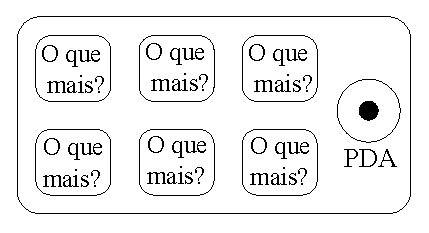
\includegraphics[height=1.00in]{figs2/pda.eps}}
\afterfig

Programadores adicionam um sistema operacional e um conjunto de
aplicações ao hardware e nós terminamos com um Assistente
Pessoal Digital que é muito útil e capaz de nos ajudar a fazer
diversas coisas.
%Programmers add an operating system and a set of applications
%to the hardware and we end up with a Personal Digital
%Assistant that is quite helpful and capable of helping
%us do many different things.

Nossos computadores são rápidos, tem vasta quantidade de memória
e podem ser muito úteis para nós, somente se conhecermos a linguagem
falada para explicar para um computador o que nós gostaríamos
de fazer ``em seguida''. Se nós conhecemos esta linguagem, nós
podemos pedir ao computador para fazer tarefas repetitivas a
nosso favor. Curiosamente, as coisas que os computadores
podem fazer melhor são frequentemente aquelas coisas que humanos
acham chatas e entediantes.
%Our computers are fast and have vast amounts of memory and
%could be very helpful to us if we only knew the language to
%speak to explain to the computer what we would like it to
%``do next''.  If we knew this language, we could tell the
%computer to do tasks on our behalf that were repetitive.
%Interestingly, the kinds of things computers can do best
%are often the kinds of things that we humans find boring
%and mind-numbing.

Por exemplo, olhe para os três primeiros parágrafos deste
capítulo e me diga qual é a palavra mais usada e quantas
vezes. Contá-las é muito doloroso porque
não é o tipo de problema que mentes humanas foram feitas para
resolver. Para um computador o oposto é verdade, ler e entender o texto
de um pedaço de papel é difícil, mas contar palavras dizendo a
você quantas vezes ela aparece é muito fácil:
%For example, look at the first three paragraphs of this
%chapter and tell me the most commonly used word and how
%many times the word is used.  While you were able to read
%and understand the words in a few seconds, counting them
%is almost painful because it is not the kind of problem
%that human minds are designed to solve.  For a computer
%the opposite is true, reading and understanding text
%from a piece of paper is hard for a computer to do
%but counting the words and telling you how many times
%the most used word was used is very easy for the
%computer:

\beforeverb
\begin{verbatim}
python palavras.py
Digite o nome do arquivo: palavras.txt
para 16
\end{verbatim}
\afterverb
%\beforeverb
%\begin{verbatim}
%python words.py
%Enter file:words.txt
%to 16
%\end{verbatim}
%\afterverb

Nosso ``assistente de análise pessoal de informações'' rapidamente
conta para nós que a palavra ``para'' foi utilizada dezesseis vezes nos
primeiros três parágrafos deste capítulo.
%Our ``personal information analysis assistant'' quickly
%told us that the word ``to'' was used sixteen times in the
%first three paragraphs of this chapter.

Este fato de que os computadores são bons em coisas
que humanos não são é a razão pela qual você precisa tornar-se
qualificado em falar a ``linguagem do computador''. Uma vez
que você aprende esta nova linguagem, pode delegar tarefas
mundanas para o seu parceiro (o computador), ganhando mais tempo
para fazer coisas que você foi especialmente adaptado para fazer. Você agrega
criatividade, intuição e originalidade para o seu parceiro.
%This very fact that computers are good at things
%that humans are not is why you need to become
%skilled at talking ``computer language''.  Once you learn
%this new language, you can delegate mundane tasks
%to your partner (the computer), leaving more time
%for you to do the
%things that you are uniquely suited for.  You bring
%creativity, intuition, and inventiveness to this
%partnership.

\section{Criatividade e motivação}
%\section{Creativity and motivation}


Embora este livro não se destine a programadores profissionais, programação
profissional pode ser um trabalho muito gratificante, tanto financeiramente
quanto pessoalmente. Construir programas úteis, elegantes, inteligentes para
que outros utilizem é uma atividade criativa. Seu computador ou assistente
pessoal digital (PDA) geralmente contém muitos programas diferentes feitos por
diversos grupos de programadores, todos competindo por sua atenção e seu
interesse. Eles tentam dar o seu melhor para atender suas necessidades e dar a
você uma boa experiência de usabilidade no processo. Em algumas situações,
quando você executa um trecho de software, os programadores são diretamente
recompensados por sua escolha.
%While this book is not intended for professional programmers, professional
%programming can be a very rewarding job both financially and personally.
%Building useful, elegant, and clever programs for others to use is a very
%creative activity.  Your computer or Personal Digital Assistant (PDA)
%usually contains many different programs from many different groups of
%programmers, each competing for your attention and interest.  They try
%their best to meet your needs and give you a great user experience in the
%process.   In some situations, when you choose a piece of software, the
%programmers are directly compensated because of your choice.

Se nós pensarmos em programas como resultado criativo de grupos de programadores,
então talvez a figura a seguir seja uma versão mais sensata de nosso PDA:
%If we think of programs as the creative output of groups of programmers,
%perhaps the following figure is a more sensible version of our PDA:

\beforefig
\centerline{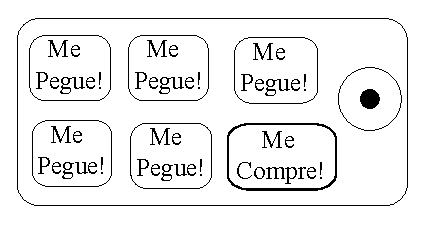
\includegraphics[height=1.00in]{figs2/pda2.eps}}
\afterfig

Por enquanto, nossa motivação primária não é ganhar dinheiro ou agradar usuários finais, mas sermos mais produtivos na manipulação de dados e informações
que nós encontraremos em nossas vidas.
Quando você começar, você será tanto o programador quanto o usuário final de seus
programas. Conforme você ganhar habilidades como programador e melhorar a criatividade
em seus próprios programas, mais você pode pensar em programar para os outros.
%For now, our primary motivation is not to make money or please end users, but
%instead for us to be more productive in handling the data and
%information that we will encounter in our lives.
%When you first start, you will be both the programmer and the end user of
%your programs.  As you gain skill as a programmer and
%programming feels more creative to you, your thoughts may turn
%toward developing programs for others.
%

\section{Arquitetura física do Computador - Hardware}
\index{hardware}
\index{hardware!arquitetura}
%\section{Computer hardware architecture}
%\index{hardware}
%\index{hardware!architecture}
%

Antes de começar a estudar a linguagem, nós falamos
em dar instruções aos computadores para desenvolver software,
nós precisamos aprender um pouco mais sobre como os computadores
são construídos. Se você desmontar seu computador ou celular e olhar
por dentro, você encontrará as seguintes partes:
%Before we start learning the language we
%speak to give instructions to computers to
%develop software, we need to learn a small amount about
%how computers are built.  If you were to take
%apart your computer or cell phone and look deep
%inside, you would find the following parts:
%

\beforefig
\centerline{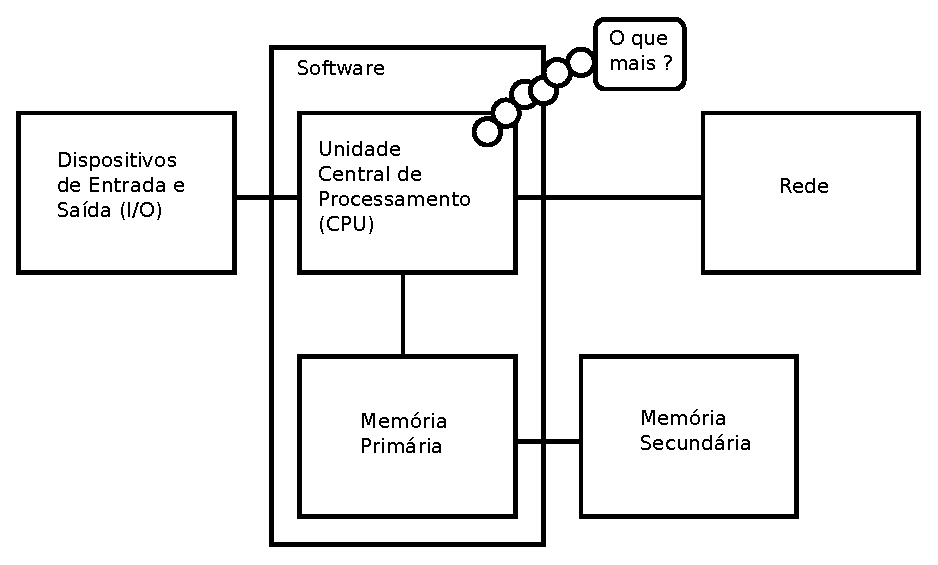
\includegraphics[height=2.50in]{figs2/arch.eps}}
\afterfig
%\beforefig
%\centerline{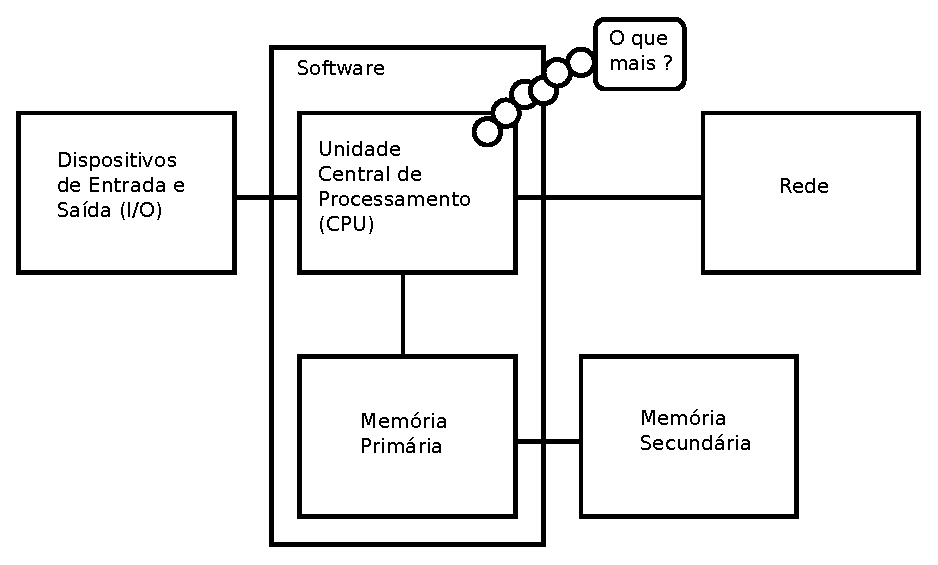
\includegraphics[height=2.50in]{figs2/arch.eps}}
%\afterfig
%

As definições resumidas destas partes são:
%The high-level definitions of these parts are as follows:
%

\begin{itemize}
%\begin{itemize}
%

\item A {\bf Unidade Central de Processamento} (ou CPU) é
a parte do computador que é feita para sempre te perguntar:
``O que mais ?'' Se seu computador possui uma frequência de
3.0 Gigahertz, significa que a CPU irá te perguntar ``O que mais ?''
três bilhões de vezes por segundo. Você irá aprender como conversar
tão rápido com a CPU.
%\item The {\bf Central Processing Unit} (or CPU) is
%the part of the computer that is built to be obsessed
%with ``what is next?''  If your computer is rated
%at 3.0 Gigahertz, it means that the CPU will ask ``What next?''
%three billion times per second.  You are going to have to
%learn how to talk fast to keep up with the CPU.
%

\item A {\bf Memória Principal} é utilizada para armazenar informação
que a CPU precisa com muita pressa. A memória principal é aproximadamente
tão rápida quanto a CPU. Mas a informação armazenada na memória principal
se perde quando o computador é desligado (volátil).
%\item The {\bf Main Memory} is used to store information
%that the CPU needs in a hurry.  The main memory is nearly as
%fast as the CPU.  But the information stored in the main
%memory vanishes when the computer is turned off.
%

\item A {\bf Memória Secundária} é também utilizada para armazenar
informação, mas ela é muito mais lenta que a memória principal.
A vantagem da memória secundária é que ela pode armazenar informação
que não se perde quando o computador é desligado. Exemplos de memória
secundária são discos rígidos (HD), pen drives, cartões de memória (sd card)
(tipicamente) encontradas no formato de USB e portáteis.
%\item The {\bf Secondary Memory} is also used to store
%information, but it is much slower than the main memory.
%The advantage of the secondary memory is that it can
%store information even when there is no power to the
%computer.  Examples of secondary memory are disk drives
%or flash memory (typically found in USB sticks and portable
%music players).
%

\item Os {\bf Dispositivos de Entrada e Saídas} são simplesmente
nosso monitor (tela), teclado, mouse, microfone, caixa de som, touchpad, etc.
Eles são todas as formas com as quais interagimos com o computador.
%\item The {\bf Input and Output Devices} are simply our
%screen, keyboard, mouse, microphone, speaker, touchpad, etc.
%They are all of the ways we interact with the computer.
%

\item Atualmente, a maioria dos computadores tem uma
{\bf Conexão de Rede} para buscar informação em uma rede.
Nós podemos pensar a rede como um lugar muito lento para armazenar
e buscar dados que podem não estar ``disponíveis''. Em essência,
a rede é mais lenta e às vezes parece uma forma não confiável de
{\bf Memória Secundária}.
%\item These days, most computers also have a
%{\bf Network Connection} to retrieve information over a network.
%We can think of the network as a very slow place to store and
%retrieve data that might not always be ``up''.  So in a sense,
%the network is a slower and at times unreliable form of
%{\bf Secondary Memory}.
%

\end{itemize}
%\end{itemize}
%

É melhor deixar a maior parte dos detalhes de como estes componentes funcionam para
os construtores dos computadores. Isso nos ajuda a ter alguma terminologia
que podemos utilizar para conversar sobre essas partes conforme escrevemos nossos programas.
%While most of the detail of how these components work is best left
%to computer builders, it helps to have some terminology
%so we can talk about these different parts as we write our programs.
%

Como um programador, seu trabalho é usar e orquestrar
cada um destes recursos para resolver um problema que você precisa resolver
e analisar os dados que você obtém da solução. Como um programador você irá
``conversar'' com a CPU e contar a ela o que fazer em um próximo passo.
Algumas vezes você irá dizer à CPU para usar a memória principal, a memória
secundária, a rede ou os dispositivos de entrada e saída.
%As a programmer, your job is to use and orchestrate
%each of these resources to solve the problem that you need to solve
%and analyze the data you get from the solution.  As a programmer you will
%mostly be ``talking'' to the CPU and telling it what to
%do next.  Sometimes you will tell the CPU to use the main memory,
%secondary memory, network, or the input/output devices.
%

\beforefig
\centerline{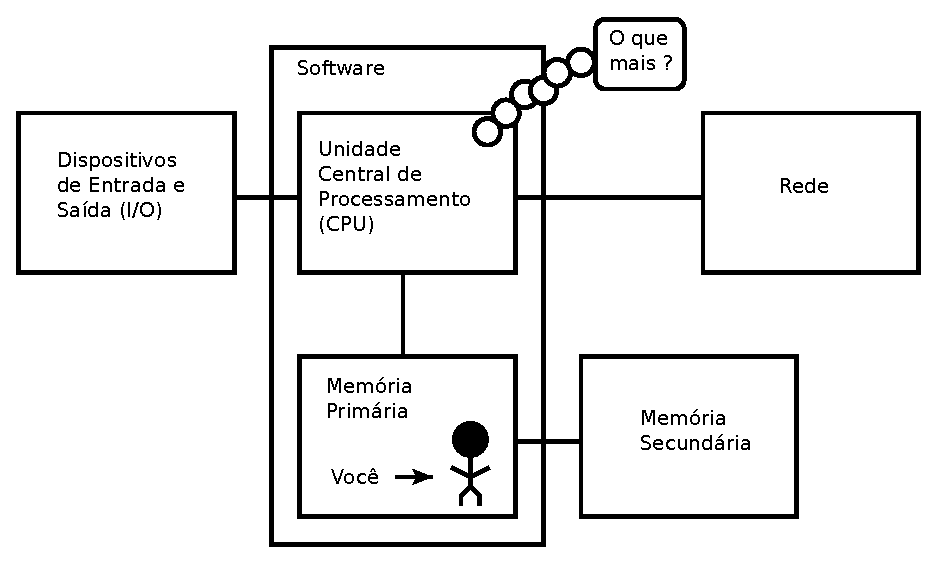
\includegraphics[height=2.50in]{figs2/arch2.eps}}
\afterfig
%\beforefig
%\centerline{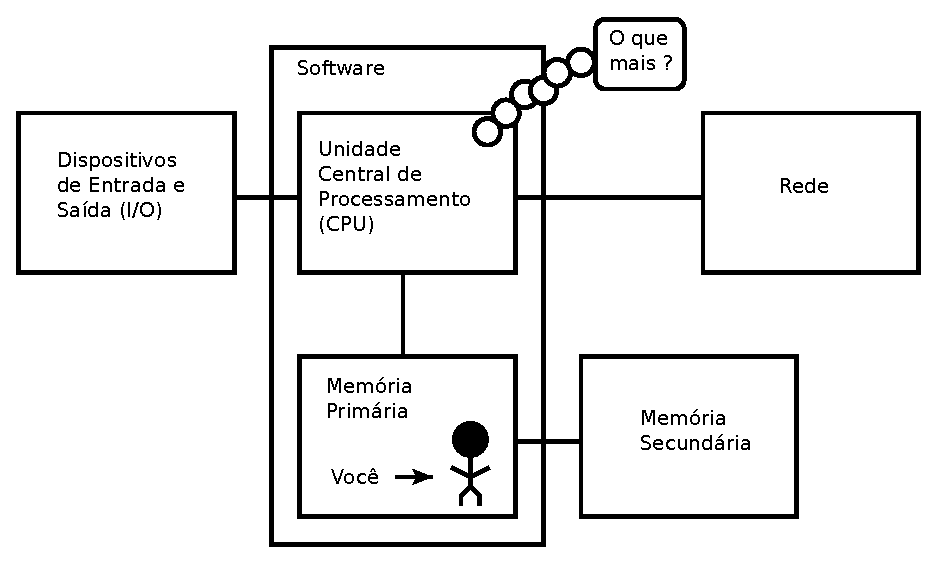
\includegraphics[height=2.50in]{figs2/arch2.eps}}
%\afterfig
%

Você precisa ser a pessoa que responde à pergunta ``O que mais ?''
para a CPU. Mas seria muito desconfortável se você fosse encolhido
para uma altura de apenas 5 mm e inserido dentro de um computador
e ainda ter que responder uma pergunta três bilhões de vezes por segundo.
Então, ao invés disso, você deve escrever suas instruções previamente.
Nós chamamos essas instruções armazenadas de {\bf programa} e o
ato de escrever essas instruções e garantir que essas estejam corretas de {\bf programação}.
%You need to be the person who answers the CPU's ``What next?''
%question.  But it would be very uncomfortable to shrink you
%down to 5mm tall and insert you into the computer just so you
%could issue a command three billion times per second.  So instead,
%you must write down your instructions in advance.
%We call these stored instructions a {\bf program} and the act
%of writing these instructions down and getting the instructions to
%be correct {\bf programming}.
%
\section{Entendendo programação}
%\section{Understanding programming}
%

No restante deste livro, nós iremos tentar fazer de você uma pessoa
com habilidades na arte da programação. No final você será um
{\bf programador}, no entanto não um programador profissional, mas
pelo menos você terá os conhecimentos para analisar os problemas
de dados/informações e desenvolver um programa para resolver tais
problemas.
%In the rest of this book, we will try to turn you into a person
%who is skilled in the art of programming.  In the end you will be a
%{\bf programmer} --- perhaps not a professional programmer, but
%at least you will have the skills to look at a data/information
%analysis problem and develop a program to solve the problem.
%

\index{resolução de problemas}
%\index{problem solving}
%

Resumidamente, você precisa de duas qualidades para ser um programador:
%In a sense, you need two skills to be a programmer:
%

\begin{itemize}
%\begin{itemize}
%

\item Primeiramente, você precisa conhecer uma linguagem de programação (Python) -
você precisa conhecer o vocabulário e a gramática. Você precisa saber
pronunciar as palavras desta nova linguagem corretamente e conhecer como construir
``sentenças'' bem formadas nesta linguagem.
%\item First, you need to know the programming language (Python) -
%you need to know the vocabulary and the grammar.  You need to be able
%to spell the words in this new language properly and know how to construct
%well-formed ``sentences'' in this new language.
%

\item Segundo, você precisa ``contar uma estória''. Na escrita da estória,
você combina palavras e sentenças para convencer o leitor.
É necessário qualidade e arte na construção da estória, adquiri-se
isso através da prática de contar estórias e obter um feedback.
Na programação, nosso programa é a ``estória'' e o problema que você
quer resolver é a ``idéia''.
%\item Second, you need to ``tell a story''.  In writing a story,
%you combine words and sentences to convey an idea to the reader.
%There is a skill and art in constructing the story, and skill in
%story writing is improved by doing some writing and getting some
%feedback.  In programming, our program is the ``story'' and the
%problem you are trying to solve is the ``idea''.
%

\end{itemize}
%\end{itemize}
%

Uma vez que você aprende uma linguagem de programação, como o Python, você irá
achar muito mais fácil aprender uma segunda linguagem de programação, tal como
JavaScript ou C++. A nova linguagem de programação possuirá um vocabulário
e gramática bastante diferente, mas as habilidades na resolução do problemas
serão as mesmas em qualquer linguagem.
%Once you learn one programming language such as Python, you will
%find it much easier to learn a second programming language such
%as JavaScript or C++.  The new programming language has very different
%vocabulary and grammar but the problem-solving skills
%will be the same across all programming languages.
%

Você aprenderá o ``vocabulário'' e ``sentenças'' do Python rapidamente.
Levará muito tempo para você tornar-se hábil em escrever programas coerentes
para resolver um novo problema. Nós ensinamos programação assim como ensinamos
a escrever. Nós leremos e explicaremos programas, nós escreveremos programas
simples, e então nós aumentaremos a complexidade dos programas ao longo do tempo.
Em algum momento, você ``deslancha'' e vê os padrões por si próprio e pode visualizar
com maior naturalidade como escrever um programa para resolver o problema. Uma
vez que você chega neste ponto, programar torna-se um processo muito agradável e
criativo.
%You will learn the ``vocabulary'' and ``sentences'' of Python pretty quickly.
%It will take longer for you to be able to write a coherent program
%to solve a brand-new problem.  We teach programming much like we teach
%writing.  We start reading and explaining programs, then we write
%simple programs, and then we write increasingly complex programs over time.
%At some point you ``get your muse'' and see the patterns on your own
%and can see more naturally how to take a problem and
%write a program that solves that problem.  And once you get
%to that point, programming becomes a very pleasant and creative process.
%

Nós iniciamos com o vocabulário e a estrutura de programas em Python. Seja paciente
com os exemplos simples, relembre quando você iniciou a leitura pela primeira vez.
%We start with the vocabulary and structure of Python programs.  Be patient
%as the simple examples remind you of when you started reading for the first
%time.
%

\section{Palavras e Sentenças}
\index{linguagem de programação}
\index{linguagem!programação}
%\section{Words and sentences}
%\index{programming language}
%\index{language!programming}
%

Diferentemente dos idiomas humanos, o vocabulário do Python é atualmente muito pequeno.
Nós chamamos esse ``vocabulário'' de ``palavras reservadas''. Estas palavras tem
um significado especial no Python. Quando o Python encontra estas palavras em um
programa, elas possuem um e somente um significado para o Python. Quando você
escrever seus programas você irá definir suas próprias palavras com significado,
são chamadas {\bf variáveis}. Você pode escolher muitos nomes diferentes para
as suas variáveis, mas você não pode usar qualquer palavra reservada do Python
como o nome de uma variável.
%Unlike human languages, the Python vocabulary is actually pretty small.
%We call this ``vocabulary'' the ``reserved words''.  These are words that
%have very special meaning to Python.  When Python sees these words in
%a Python program, they have one and only one meaning to Python.  Later
%as you write programs you will make up your own words that have meaning to
%you called {\bf variables}.   You will have great latitude in choosing
%your names for your variables, but you cannot use any of Python's
%reserved words as a name for a variable.
%

Quando nós treinamos um cachorro, nós usamos palavras especiais, tais como:
``sentado'', ``fique'' e ``traga''. Quando você conversar com cachorros e
não usar qualquer uma dessas palavras reservadas, eles ficarão olhando para você
com um olhar curioso até que você diga uma palavra reservada.
Por exemplo, se você disser: ``Eu desejo que mais pessoas possam caminhar para
melhorar a sua saúde'', o que os cachorros vão ouvir será:
``blah blah blah {\bf caminhar} blah blah blah blah.''
Isto porque ``caminhar'' é uma palavra reservada na linguagem dos cachorros. Muitos
podem sugerir que a linguagem entre humanos e gatos não tem palavras
reservadas\footnote{\url{http://xkcd.com/231/}}.
%When we train a dog, we use special words like
%``sit'', ``stay'', and ``fetch''.  When you talk to a dog and
%don't use any of the reserved words, they just look at you with a
%quizzical look on their face until you say a reserved word.
%For example, if you say,
%``I wish more people would walk to improve their overall health'',
%what most dogs likely hear is,
%``blah blah blah {\bf walk} blah blah blah blah.''
%That is because ``walk'' is a reserved word in dog language.  Many
%might suggest that the language between humans and cats has no
%reserved words\footnote{\url{http://xkcd.com/231/}}.
%

As palavras reservadas na linguagem pelas quais os humanos conversam com o
Python, incluem as seguintes:
%The reserved words in the language where humans talk to
%Python include the following:
%

\beforeverb
\begin{verbatim}
and       del       from      not       while
as        elif      global    or        with
assert    else      if        pass      yield
break     except    import    print
class     exec      in        raise
continue  finally   is        return
def       for       lambda    try
\end{verbatim}
\afterverb
%

É isso, e ao contrário do cachorro, o Python é completamente treinado.
Quando você diz ``try'', o Python irá tentar todas as vezes que você pedir
sem desobedecer.
%That is it, and unlike a dog, Python is already completely trained.
%When you say ``try'', Python will try every time you say it without
%fail.
%

Nós aprenderemos as palavras reservadas e como elas são usadas mais adiante,
por enquanto nós iremos focar no equivalente ao Python de ``falar'' (na
linguagem humano-para-cachorro). Uma coisa legal sobre pedir ao Python para falar
é que nós podemos até mesmo pedir o que nós queremos através de uma mensagem
entre aspas:
%We will learn these reserved words and how they are used in good time,
%but for now we will focus on the Python equivalent of ``speak'' (in
%human-to-dog language).  The nice thing about telling Python to speak
%is that we can even tell it what to say by giving it a message in quotes:
%

\beforeverb
\begin{verbatim}
print 'Hello world!'
\end{verbatim}
\afterverb
%

E finalmente nós escrevemos a nossa primeira sentença sintaticamente correta em Python.
Nossa sentença inicia com uma palavra reservada {\bf print} seguida por
uma cadeia de caracteres textuais de nossa escolha entre aspas simples.
%And we have even written our first syntactically correct Python sentence.
%Our sentence starts with the reserved word {\bf print} followed
%by a string of text of our choosing enclosed in single quotes.
%

\section{Conversando com Python}
%\section{Conversing with Python}
%

Agora que você tem uma palavra e uma simples sentença que nós conhecemos em Python,
nós precisamos saber como iniciar uma conversação com Python para testar
nossas habilidades na nova linguagem.
%Now that we have a word and a simple sentence that we know in Python,
%we need to know how to start a conversation with Python to test
%our new language skills.
%

Antes de você conversar com o Python, você deve primeiramente instalar o programa
Python em seu computador e aprender como inicializá-lo. Isto é muita informação
para este capítulo, então eu sugiro que você consulte \url{www.pythonlearn.com}
onde se encontra instruções e screencasts de preparação e inicialização do Python
em sistemas Windows e Macintosh. Em algum momento, você estará no interpretador
Python, executando o modo interativo e aparecerá algo assim:
%Before you can converse with Python, you must first install the Python
%software on your computer and learn how to start Python on your
%computer.  That is too much detail for this chapter so I suggest
%that you consult \url{www.pythonlearn.com} where I have detailed
%instructions and screencasts of setting up and starting Python
%on Macintosh and Windows systems.  At some point, you will be in
%a terminal or command window and you will type {\bf python} and
%the Python interpreter will start executing in interactive mode
%and appear somewhat as follows:

\index{modo interativo}

\beforeverb
\begin{verbatim}
Python 2.6.1 (r261:67515, Jun 24 2010, 21:47:49)
[GCC 4.2.1 (Apple Inc. build 5646)] on darwin
Type "help", "copyright", "credits" or "license" for more information.
>>>
\end{verbatim}
\afterverb
%

O prompt {\tt >>>} é a forma do interpretador Python perguntar o que você deseja:
``O que você quer que eu faça agora?'' Python está pronto para ter uma conversa
com você. Tudo o que você deve conhecer é como falar a linguagem Python.
%The {\tt >>>} prompt is the Python interpreter's way of asking you, ``What
%do you want me to do next?''  Python is ready to have a conversation with
%you.  All you have to know is how to speak the Python language.
%

Digamos, por exemplo, que você não conhece nem mesmo as mais simples palavras
ou sentenças da linguagem Python. Você pode querer usar a linha padrão que os
astronautas usam quando eles estão em uma terra distante do planeta e tentam falar com os habitantes do planeta:
%Let's say for example that you did not know even the simplest Python language
%words or sentences. You might want to use the standard line that astronauts
%use when they land on a faraway planet and try to speak with the inhabitants
%of the planet:
%

\beforeverb
\begin{verbatim}
>>> Eu venho em paz, por favor me leve para o seu líder
  File "<stdin>", line 1
    Eu venho em paz, por favor me leve para o seu líder
         ^
SyntaxError: invalid syntax
>>>
\end{verbatim}
\afterverb
%\beforeverb
%\begin{verbatim}
%>>> I come in peace, please take me to your leader
%  File "<stdin>", line 1
%    I come in peace, please take me to your leader
%         ^
%SyntaxError: invalid syntax
%>>>
%\end{verbatim}
%\afterverb
%%

Isto não deu muito certo. A menos que você pense algo rapidamente,
os habitantes do planeta provavelmente irão apunhalá-lo com uma lança,
colocá-lo em um espeto, assá-lo no fogo e comê-lo no jantar.
%This is not going so well.  Unless you think of something quickly,
%the inhabitants of the planet are likely to stab you with their spears,
%put you on a spit, roast you over a fire, and eat you for dinner.
%

A sorte é que você trouxe uma cópia deste livro em sua viagem, e caiu
exatamente nesta página, tente novamente:
%Luckily you brought a copy of this book on your travels, and you thumb to
%this very page and try again:
%

\beforeverb
\begin{verbatim}
>>> print 'Ola Mundo!'
Ola Mundo!
\end{verbatim}
\afterverb

%\beforeverb
%\begin{verbatim}
%>>> print 'Hello world!'
%Hello world!
%\end{verbatim}
%\afterverb
%%

Isso parece bem melhor, então você tenta se comunicar um pouco
mais:
%This is looking much better, so you try to communicate some
%more:
%

\beforeverb
\begin{verbatim}
>>> print 'Voce deve ser um Deus lendario que veio do ceu'
Voce deve ser um Deus lendario que veio do ceu
>>> print 'Nos estivemos esperando voce por um longo tempo'
Nos estivemos esperando voce por um longo tempo
>>> print 'Nossa lenda nos conta que voce seria muito apetitoso com mostarda'
Nossa lenda nos conta que voce seria muito apetitoso com mostarda
>>> print 'Nos teremos uma festa hoje a noite a menos que voce diga
  File "<stdin>", line 1
    print 'Nos teremos uma festa hoje a noite a menos que voce diga
                                                                  ^
SyntaxError: EOL while scanning string literal
>>>
\end{verbatim}
\afterverb

%\beforeverb
%\begin{verbatim}
%>>> print 'You must be the legendary god that comes from the sky'
%You must be the legendary god that comes from the sky
%>>> print 'We have been waiting for you for a long time'
%We have been waiting for you for a long time
%>>> print 'Our legend says you will be very tasty with mustard'
%Our legend says you will be very tasty with mustard
%>>> print 'We will have a feast tonight unless you say
%  File "<stdin>", line 1
%    print 'We will have a feast tonight unless you say
%                                                     ^
%SyntaxError: EOL while scanning string literal
%>>>
%\end{verbatim}
%\afterverb
%%

A conversa foi bem por um momento, até que você cometeu o
pequeno erro no uso da linguagem e o Python trouxe a lança
de volta.
%The conversation was going so well for a while and then you
%made the tiniest mistake using the Python language and Python
%brought the spears back out.
%

Até o momento, você deve ter percebido que o Python
é incrivelmente complexo, poderoso e muito exigente em relação
à sintaxe que você utiliza para se comunicar com ele, Python {\em não}
é inteligente. Você está na verdade tendo uma conversa com você mesmo,
mas usando uma sintaxe apropriada.
%At this point, you should also realize that while Python
%is amazingly complex and powerful and very picky about
%the syntax you use to communicate with it, Python is {\em
%not} intelligent.  You are really just having a conversation
%with yourself, but using proper syntax.
%

De certa forma, quando você usa um programa escrito por alguém,
a conversa ocorre entre você e os programadores, neste caso o Python
atuou como um intermediário. Python é uma forma para que os criadores de
programas se expressem sobre como uma conversa deve proceder. E em poucos
capítulos, você será um dos programadores usando Python para conversar com
os usuários de seus programas.
%In a sense, when you use a program written by someone else
%the conversation is between you and those other
%programmers with Python acting as an intermediary.  Python
%is a way for the creators of programs to express how the
%conversation is supposed to proceed.  And
%in just a few more chapters, you will be one of those
%programmers using Python to talk to the users of your program.
%

Antes de sairmos da nossa primeira conversa com o interpretador
do Python, você deve conhecer o modo correto de dizer ``ate-logo''
quando interagir com os habitantes do Planeta Python.
%Before we leave our first conversation with the Python
%interpreter, you should probably know the proper way
%to say ``good-bye'' when interacting with the inhabitants
%of Planet Python:
%

\beforeverb
\begin{verbatim}
>>> ate-logo
Traceback (most recent call last):
  File "<stdin>", line 1, in <module>
NameError: name 'ate' is not defined

>>> se voce nao se importa, eu preciso ir embora
  File "<stdin>", line 1
    se voce nao se importa, eu preciso ir embora
          ^
SyntaxError: invalid syntax

>>> quit()
\end{verbatim}
\afterverb
%

%\beforeverb
%\begin{verbatim}
%>>> good-bye
%Traceback (most recent call last):
%  File "<stdin>", line 1, in <module>
%NameError: name 'good' is not defined
%
%>>> if you don't mind, I need to leave
%  File "<stdin>", line 1
%    if you don't mind, I need to leave
%             ^
%SyntaxError: invalid syntax
%
%>>> quit()
%\end{verbatim}
%\afterverb
%%

Você pode perceber que o erro é diferente nas duas primeiras
tentativas incorretas. No primeiro erro, por tratar-se de uma
palavra simples, o Python não pode encontrar nenhuma função ou
variável com este nome. No segundo erro, existe um erro de sintaxe,
não sendo reconhecida a frase como válida.
%You will notice that the error is different for the first two
%incorrect attempts.   The second error is different because
%{\bf if} is a reserved word and Python saw the reserved word
%and thought we were trying to say something but got the syntax
%of the sentence wrong.
%

O jeito correto de se dizer ``ate-logo'' para o Python é
digitar {\bf quit()} no prompt do interpretador interativo.
É provável que você tenha perdido certo tempo tentado fazer isso,
ter um livro em mãos irá tornar as coisas mais fáceis e
pode ser bastante útil.
%The proper way to say ``good-bye'' to Python is to enter
%{\bf quit()} at the interactive chevron {\tt >>>} prompt.
%It would have probably taken you quite a while to guess that
%one, so having a book handy probably will turn out
%to be helpful.
%

\section{Terminologia: interpretador e compilador}
%\section{Terminology: interpreter and compiler}
%

Python é uma linguagem de {\bf alto nível} cujo objetivo é ser
relativamente fácil para humanos lerem e escreverem e para computadores
lerem e processarem. Outras linguagens de alto nível incluem Java, C++,
PHP, Ruby, Basic, Perl, JavaScript, e muito mais. O atual hardware
dentro da Unidade Central de Processamento (CPU) não é capaz de entender
nenhum destes comando em alto nível.
%Python is a {\bf high-level} language intended to be relatively
%straightforward for humans to read and write and for computers
%to read and process.  Other high-level languages include Java, C++,
%PHP, Ruby, Basic, Perl, JavaScript, and many more.  The actual hardware
%inside the Central Processing Unit (CPU) does not understand any
%of these high-level languages.
%

A CPU entende a linguagem que chamamos de {\bf linguagem de máquina}. Linguagem
de máquina é muito simples e francamente cansativa de se escrever porque ela é
representada em zeros e uns:
%The CPU understands a language we call {\bf machine language}.  Machine
%language is very simple and frankly very tiresome to write because it
%is represented all in zeros and ones:
%

\beforeverb
\begin{verbatim}
01010001110100100101010000001111
11100110000011101010010101101101
...
\end{verbatim}
\afterverb
%\beforeverb
%\begin{verbatim}
%01010001110100100101010000001111
%11100110000011101010010101101101
%...
%\end{verbatim}
%\afterverb
%%

Linguagem de máquina parece simples olhando-se de um modo superficial,
dado que são apenas zeros e uns, mas sua sintaxe é muito mais complexa
e mais intrincada que o Python. Poucos programadores escrevem em linguagem de
máquina. Ao invés disso, nós usamos vários tradutores para permitir que os
programadores escrevam em linguagem de máquina a partir de linguagens de alto nível como o Python ou o JavaScript. Essas linguagens convertem os programas
para linguagem de máquina que, desse modo, são executados pela CPU.
%Machine language seems quite simple on the surface, given that there
%are only zeros and ones, but its syntax is even more complex
%and far more intricate than Python.  So very few programmers ever write
%machine language.  Instead we build various translators to allow
%programmers to write in high-level languages like Python or JavaScript
%and these translators convert the programs to machine language for actual
%execution by the CPU.
%

Visto que linguagem de máquina é vinculada ao hardware do computador,
linguagem de máquina não é {\bf portável} entre diferentes tipos de hardware.
Programas que foram escritos em linguagens de alto nível podem mover-se
entre diferentes computadores usando um interpretador diferente em cada máquina
ou então recompilando o código para criar uma versão de linguagem de máquina do
programa para a nova máquina.
%Since machine language is tied to the computer hardware, machine language
%is not {\bf portable} across different types of hardware.  Programs written in
%high-level languages can be moved between different computers by using a
%different interpreter on the new machine or recompiling the code to create
%a machine language version of the program for the new machine.
%

Os tradutores das linguagens de programação se enquadram em duas
características gerais:
(1) interpretadores e (2) compiladores
%These programming language translators fall into two general categories:
%(1) interpreters and (2) compilers.
%

Um {\bf interpretador} lê o código fonte de um programa da forma como foi escrito
pelo programador, analisa, e interpreta as instruções em tempo de
execução. Python é um interpretador e quando ele está rodando Python no modo
interativo, nós podemos digitar uma linha de Python (uma sentença) e o Python a
processa imediatamente e está pronto para receber outra linha de Python.
%An {\bf interpreter} reads the source code of the program as written by the
%programmer, parses the source code, and interprets the instructions on the fly.
%Python is an interpreter and when we are running Python interactively,
%we can type a line of Python (a sentence) and Python processes it immediately
%and is ready for us to type another line of Python.
%

Algumas das linhas de Python diz a ele que você quer armazenar algum valor
para resgatar depois. Nós precisamos dar um nome para um valor de forma que possa
ser armazenado e resgatado através deste nome simbólico. Nós usamos o termo
{\bf variável} para se referir aos apelidos que nós demos ao dado que foi armazenado.
%Some of the lines of Python tell Python that you want it to remember some
%value for later.   We need to pick a name for that value to be remembered and
%we can use that symbolic name to retrieve the value later.  We use the
%term {\bf variable} to refer to the labels we use to refer to this stored data.
%

\beforeverb
\begin{verbatim}
>>> x = 6
>>> print x
6
>>> y = x * 7
>>> print y
42
>>>
\end{verbatim}
\afterverb
%\beforeverb
%\begin{verbatim}
%>>> x = 6
%>>> print x
%6
%>>> y = x * 7
%>>> print y
%42
%>>>
%\end{verbatim}
%\afterverb
%%

Neste exemplo, nós pedimos ao Python para armazenar o valor seis e usar um apelido {\bf x}, de modo a nós podermos resgatar o valor mais tarde. Nós verificamos que o Python realmente
lembrou dos valores quando usamos a função {\bf print}. Então nós perguntamos ao Python
para resgatar {\bf x}, multiplicá-lo por sete e armazenar de novo em uma variável {\bf y}.
Então nós pedimos ao Python para exibir o valor corrente em {\bf y}.
%In this example, we ask Python to remember the value six and use the label {\bf x}
%so we can retrieve the value later.   We verify that Python has actually remembered
%the value using {\bf print}. Then we ask Python to retrieve {\bf x} and multiply
%it by seven and put the newly computed value in {\bf y}.  Then we ask Python to print out
%the value currently in {\bf y}.
%

Mesmo que nós digitemos estes comandos em uma única linha de Python por vez, o Python
está processando elas em sequência, mantendo a ordem, de forma que as
instruções seguintes consigam recuperar os dados criados pelas anteriores. Nós escrevemos
nosso primeiro parágrafo simples com quatro sentenças com uma ordem lógica e com um
significado.
%Even though we are typing these commands into Python one line at a time, Python
%is treating them as an ordered sequence of statements with later statements able
%to retrieve data created in earlier statements.   We are writing our first
%simple paragraph with four sentences in a logical and meaningful order.
%

É da natureza de um {\bf interpretador} ser capaz de ter uma conversa interativa, como
foi mostrado acima. Um {\bf compilador} precisa ter em mãos o programa completo em um arquivo, então ele roda um processo para traduzir um código fonte em alto nível para uma linguagem
de máquina e, em seguida, o compilador coloca o resultado deste processo em um outro arquivo
para posterior execução.
%It is the nature of an {\bf interpreter} to be able to have an interactive conversation
%as shown above.  A {\bf compiler} needs to be handed the entire program in a file, and then
%it runs a process to translate the high-level source code into machine language
%and then the compiler puts the resulting machine language into a file for later
%execution.
%

Se você está em um sistema Windows, frequentemente este programa executável em código
de máquina tem o sufixo ``.exe'' ou ``.dll'', os quais são chamados de ``executável'' ou
``biblioteca de link dinâmico'', respectivamente. Em Linux e Macintosh, não há um sufixo
que marca unicamente um arquivo como executável.
%If you have a Windows system, often these executable machine language programs have a
%suffix of ``.exe'' or ``.dll'' which stand for ``executable'' and ``dynamic link
%library'' respectively.  In Linux and Macintosh, there is no suffix that uniquely marks
%a file as executable.
%

Se você abrir um arquivo executável em um editor de texto, verá algo completamente
doido e ilegível.
%If you were to open an executable file in a text editor, it would look
%completely crazy and be unreadable:
%

\beforeverb
\begin{verbatim}
^?ELF^A^A^A^@^@^@^@^@^@^@^@^@^B^@^C^@^A^@^@^@\xa0\x82
^D^H4^@^@^@\x90^]^@^@^@^@^@^@4^@ ^@^G^@(^@$^@!^@^F^@
^@^@4^@^@^@4\x80^D^H4\x80^D^H\xe0^@^@^@\xe0^@^@^@^E
^@^@^@^D^@^@^@^C^@^@^@^T^A^@^@^T\x81^D^H^T\x81^D^H^S
^@^@^@^S^@^@^@^D^@^@^@^A^@^@^@^A\^D^HQVhT\x83^D^H\xe8
....
\end{verbatim}
\afterverb
%\beforeverb
%\begin{verbatim}
%^?ELF^A^A^A^@^@^@^@^@^@^@^@^@^B^@^C^@^A^@^@^@\xa0\x82
%^D^H4^@^@^@\x90^]^@^@^@^@^@^@4^@ ^@^G^@(^@$^@!^@^F^@
%^@^@4^@^@^@4\x80^D^H4\x80^D^H\xe0^@^@^@\xe0^@^@^@^E
%^@^@^@^D^@^@^@^C^@^@^@^T^A^@^@^T\x81^D^H^T\x81^D^H^S
%^@^@^@^S^@^@^@^D^@^@^@^A^@^@^@^A\^D^HQVhT\x83^D^H\xe8
%....
%\end{verbatim}
%\afterverb
%%

Não é nada fácil ler ou escrever código de máquina, assim é bom que tenhamos
{\bf interpretadores} e {\bf compiladores} que nos permitam escrever em linguagens
de alto nível assim como o Python ou o C.
%It is not easy to read or write machine language, so it is nice that we have
%{\bf interpreters} and {\bf compilers} that allow us to write in high-level
%languages like Python or C.
%

Agora neste ponto em nossa discussão de compiladores e interpretadores, você deve
estar com algumas dúvidas sobre o funcionamento do interpretador Python. Em que
linguagem é escrito? É escrito em uma linguagem compilada? Quando nós
digitamos ``python'', o que exatamente acontece?
%Now at this point in our discussion of compilers and interpreters, you should
%be wondering a bit about the Python interpreter itself.  What language is
%it written in?  Is it written in a compiled language?  When we type
%``python'', what exactly is happening?
%

O interpretador Python é escrito em uma linguagem de alto nível chamada ``C''.
Você pode dar uma olhada no código fonte do interpretador através
do endereço \url{www.python.org} e trabalhar como você quiser com o código fonte.
Então Python é um programa compilado em uma linguagem de máquina.
Quando você instalou Python em seu computador (ou o fornecedor instalou),
você copiou um código de máquina do programa Python traduzido para o seu sistema.
Em Windows, o código de máquina executável para o Python encontra-se em um
arquivo com um nome a seguir:
%The Python interpreter is written in a high-level language called ``C''.
%You can look at the actual source code for the Python interpreter by
%going to \url{www.python.org} and working your way to their source code.
%So Python is a program itself and it is compiled into machine code.
%When you installed Python on your computer (or the vendor installed it),
%you copied a machine-code copy of the translated Python program onto your
%system.   In Windows, the executable machine code for Python itself is likely
%in a file with a name like:
%

\beforeverb
\begin{verbatim}
C:\Python27\python.exe
\end{verbatim}
\afterverb
%\beforeverb
%\begin{verbatim}
%C:\Python27\python.exe
%\end{verbatim}
%\afterverb
%%

Isso é mais do que você realmente precisa conhecer para ser um programador Python, mas
às vezes, isso ajuda a entender questões que intrigam justamente no início.
%That is more than you really need to know to be a Python programmer, but
%sometimes it pays to answer those little nagging questions right at
%the beginning.
%

\section{Escrevendo um programa}
%\section{Writing a program}
%

Digitar comandos em um Interpretador Python é uma boa maneira de experimentar
as características da linguagem, mas isto não é recomendado para resolver
problemas mais complexos.
%Typing commands into the Python interpreter is a great way to experiment
%with Python's features, but it is not recommended for solving more complex problems.
%

Quando nós queremos escrever um programa,
usamos um editor de texto para escrever as instruções Python em um arquivo,
o qual chamamos de {\bf script}. Por convenção,
scripts Python tem nomes que terminam com {\tt .py}.
%When we want to write a program,
%we use a text editor to write the Python instructions into a file,
%which is called a {\bf script}.  By
%convention, Python scripts have names that end with {\tt .py}.
%

\index{script}
%\index{script}
%

Para executar o script, você tem que dizer ao interpretador do Python
o nome do arquivo. Em uma janela de comandos Unix ou Windows, você digita
{\tt python hello.py} como a seguir:
%To execute the script, you have to tell the Python interpreter
%the name of the file.  In a Unix or Windows command window,
%you would type {\tt python hello.py} as follows:
%

\beforeverb
\begin{verbatim}
csev$ cat hello.py
print 'Ola Mundo!'
csev$ python hello.py
Ola Mundo!
csev$
\end{verbatim}
\afterverb

%\beforeverb
%\begin{verbatim}
%csev$ cat hello.py
%print 'Hello world!'
%csev$ python hello.py
%Hello world!
%csev$
%\end{verbatim}
%\afterverb
%%

O ``csev\$'' é o prompt do sistema operacional, e o ``cat hello.py'' é
para nos mostrar que o arquivo ``hello.py'' tem uma linha de programa Python para
imprimir uma string.
%The ``csev\$'' is the operating system prompt, and the ``cat hello.py'' is
%showing us that the file ``hello.py'' has a one-line Python program to print
%a string.
%

Nós chamamos o interpretador Python e pedimos a ele para ler o código fonte do
arquivo ``hello.py'' ao invés dele nos perguntar quais são as próximas linhas
de modo interativo.
%We call the Python interpreter and tell it to read its source code from
%the file ``hello.py'' instead of prompting us for lines of Python code
%interactively.
%

Você notará que não é preciso ter o {\bf quit()} no fim do programa Python
no arquivo. Quando o Python está lendo o seu código fonte de um arquivo,
ele sabe que deve parar quando chegar ao fim do arquivo.
%You will notice that there was no need to have {\bf quit()} at the end of
%the Python program in the file.   When Python is reading your source code
%from a file, it knows to stop when it reaches the end of the file.
%

\section{O que é um programa ?}
%\section{What is a program?}
%

A definição de um {\bf programa} em sua forma mais básica é uma sequência
de comandos Python que foram criados para fazer algo.
Mesmo o nosso simples script {\bf hello.py} é um programa. É um programa
de uma linha e não é particularmente útil, mas na estrita definição, é
um programa Python.
%The definition of a {\bf program} at its most basic is a sequence
%of Python statements that have been crafted to do something.
%Even our simple {\bf hello.py} script is a program.  It is a one-line
%program and is not particularly useful, but in the strictest definition,
%it is a Python program.
%

Pode ser mais fácil entender o que é um programa, imaginando qual problema ele
foi construído para resolver, e então olhar para o programa que resolve um
problema.
%It might be easiest to understand what a program is by thinking about a problem
%that a program might be built to solve, and then looking at a program
%that would solve that problem.
%

Vamos dizer que você está fazendo uma pesquisa de computação social em posts
do Facebook e está interessado nas palavras mais frequentes em uma série de posts.
Você pode imprimir o stream de posts do Facebook e debruçar-se sobre o texto
procurando pela palavra mais comum, mas pode levar um tempo longo e ser muito
propenso a erros. Você pode ser inteligente para escrever um programa Python para
tratar disso rapidamente a com acurácia, então você pode passar seu final de semana
fazendo algo divertido.
%Lets say you are doing Social Computing research on Facebook posts and
%you are interested in the most frequently used word in a series of posts.
%You could print out the stream of Facebook posts and pore over the text
%looking for the most common word, but that would take a long time and be very
%mistake prone.  You would be smart to write a Python program to handle the
%task quickly and accurately so you can spend the weekend doing something
%fun.
%

Por exemplo, olhe para o seguinte texto sobre o palhaço e o carro. Olhe para o
texto e imagine qual é a palavra mais comum e quantas vezes ela aparece:
%For example, look at the following text about a clown and a car.  Look at the
%text and figure out the most common word and how many times it occurs.
%

\beforeverb
\begin{verbatim}
O palhaço correu atrás do carro e o carro correu para a tenda
e a tenda caiu em cima do palhaço e do carro
\end{verbatim}
\afterverb
%\beforeverb
%\begin{verbatim}
%the clown ran after the car and the car ran into the tent
%and the tent fell down on the clown and the car
%\end{verbatim}
%\afterverb
%%

Então imagine que você está fazendo esta tarefa olhando para milhões de linhas
de texto. Francamente será mais rápido para você aprender Python e escrever um
programa Python para contar as palavras do que você manualmente escanear as
palavras.
%Then imagine that you are doing this task looking at millions of lines of
%text.  Frankly it would be quicker for you to learn Python and write a
%Python program to count the words than it would be to manually
%scan the words.
%

A notícia ainda melhor é que eu já fiz para você um programa simples para
encontrar a palavra mais comum em um arquivo texto. Eu escrevi, testei e agora
eu estou dando isso para que você use e economize algum tempo.
%The even better news is that I already came up with a simple program to
%find the most common word in a text file.  I wrote it,
%tested it, and now I am giving it to you to use so you can save some time.
%

\beforeverb
\begin{verbatim}
name = raw_input('Enter file:')
handle = open(name, 'r')
text = handle.read()
words = text.split()
counts = dict()

for word in words:
   counts[word] = counts.get(word,0) + 1

bigcount = None
bigword = None
for word,count in counts.items():
    if bigcount is None or count > bigcount:
        bigword = word
        bigcount = count

print bigword, bigcount
\end{verbatim}
\afterverb

%\beforeverb
%\begin{verbatim}
%name = raw_input('Enter file:')
%handle = open(name, 'r')
%text = handle.read()
%words = text.split()
%counts = dict()
%
%for word in words:
%   counts[word] = counts.get(word,0) + 1
%
%bigcount = None
%bigword = None
%for word,count in counts.items():
%    if bigcount is None or count > bigcount:
%        bigword = word
%        bigcount = count
%
%print bigword, bigcount
%\end{verbatim}
%\afterverb
%%

Você nem precisa conhecer Python para usar este programa. Você precisará chegar até o
capítulo 10 deste livro para entender completamente as impressionantes técnicas Python
que foram utilizadas para fazer o programa. Você é o usuário final, você simplesmente usa
o programa e admira-se com a inteligência e em como ela poupou seus esforços manuais.
Você simplesmente digitou o código em um arquivo chamado {\bf words.py} e executou ou então
fez o download do código fonte no site \url{http://www.pythonlearn.com/code/} e executou.
%You don't even need to know Python to use this program.  You will need to get through
%Chapter 10 of this book to fully understand the awesome Python techniques that were
%used to make the program.  You are the end user, you simply use the program and marvel
%at its cleverness and how it saved you so much manual effort.
%You simply type the code
%into a file called {\bf words.py} and run it or you download the source
%code from \url{http://www.pythonlearn.com/code/} and run it.
%

\index{programa}
%\index{program}

Este é um bom exemplo de como o Python e sua linguagem podem atuar como um intermediário
entre você (o usuário final) e eu (o programador). Python é uma forma para trocarmos
sequências úteis de instruções (i.e., programas) em uma linguagem comum que pode ser usada por
qualquer um que instalar Python em seu computador. Então nenhum de nós está conversando {\em com o Python}
mas sim nos comunicando uns com os outros {\em através} de Python.
%This is a good example of how Python and the Python language are acting as an intermediary
%between you (the end user) and me (the programmer).  Python is a way for us to exchange useful
%instruction sequences (i.e., programs) in a common language that can be used by anyone who
%installs Python on their computer.  So neither of us are talking {\em to Python},
%instead we are communicating with each other {\em through} Python.
%

\section{A construção de blocos de programas}
%\section{The building blocks of programs}
%

Em poucos capítulos, nós iremos aprender mais sobre o vocabulário, estrutura das sentenças,
dos parágrafos e da história do Python. Nós iremos aprender sobre as capacidades poderosas
do Python e como compor estas capacidades juntas para criar programas úteis.
%In the next few chapters, we will learn more about the vocabulary, sentence structure,
%paragraph structure, and story structure of Python.  We will learn about the powerful
%capabilities of Python and how to compose those capabilities together to create useful
%programs.
%

Há alguns padrões conceituais de baixo nível que nós usamos para construir programas. Estas
construções não são apenas para programas Python, elas são parte de todas as linguagens de
programação desde linguagens de baixo nível até as de alto nível.
%There are some low-level conceptual patterns that we use to construct programs.  These
%constructs are not just for Python programs, they are part of every programming language
%from machine language up to the high-level languages.
%

\begin{description}
%\begin{description}
%

\item[input:] Obter dados do ``mundo externo''. Estes dados podem ser lidos
de um arquivo ou mesmo de algum tipo de sensor como um microfone ou um GPS.
Em nossos primeiros programas, nosso input virá de um usuário que digita
dados no teclado.
%\item[input:] Get data from the ``outside world''.  This might be
%reading data from a file, or even some kind of sensor like
%a microphone or GPS.  In our initial programs, our input will come from the user
%typing data on the keyboard.
%

\item[output:] Exibe os resultados do programa em uma tela ou armazena-os
em um arquivo ou talvez os escreve em algum dispositivo tal como um
alto falante para tocar música ou falar o texto.
%\item[output:] Display the results of the program on a screen
%or store them in a file or perhaps write them to a device like a
%speaker to play music or speak text.
%

\item[execução sequencial:] Executa instruções uma após a outra
respeitando a sequência encontrada no script.
%\item[sequential execution:] Perform statements one after
%another in the order they are encountered in the script.
%

\item[execução condicional:] Avalia certas condições e as executa
ou pula a sequência de instruções.
%\item[conditional execution:] Check for certain conditions and
%then execute or skip a sequence of statements.
%

\item[execução repetitiva:] Executa algumas instruções repetitivamente,
geralmente com alguma variação.
%\item[repeated execution:] Perform some set of statements
%repeatedly, usually with
%some variation.
%

\item[reúso:] Escrever um conjunto de instruções uma única vez, dar um
nome a elas e reusar estas instruções em várias partes de um programa.
%\item[reuse:] Write a set of instructions once and give them a name
%and then reuse those instructions as needed throughout your program.
%

\end{description}
%\end{description}
%

Parece simples demais para ser verdade, e naturalmente que isto nunca
é tão simples. É como dizer que caminhar é simplesmente ``colocar
um pé na frente do outro''. A ``arte'' de escrever um programa é
compor e costurar estes elementos básicos muitas vezes para produzir
algo que seja útil aos usuários.
%It sounds almost too simple to be true, and of course it is never
%so simple.  It is like saying that walking is simply
%``putting one foot in front of the other''.  The ``art''
%of writing a program is composing and weaving these
%basic elements together many times over to produce something
%that is useful to its users.
%

O programa de contar palavras acima usa todos estes padrões exceto um.
%The word counting program above directly uses all of
%these patterns except for one.
%

\section{O que pode dar errado?}
%\section{What could possibly go wrong?}
%

Como vimos em nossa última conversa com o Python, devemos nos comunicar
de modo preciso quando escrevemos código Python. O mínimo desvio ou erro
fará com que o Python pare de executar o seu programa.
%As we saw in our earliest conversations with Python, we must
%communicate very precisely when we write Python code.  The smallest
%deviation or mistake will cause Python to give up looking at your
%program.
%

Programadores iniciantes muitas vezes tomam o fato de que o Python não deixa
espaço para erros como prova de que ele é malvado e cruel.
Enquanto o Python parece gostar de todo mundo, ele os conhece pessoalmente e
guarda um ressentimento contra eles. Devido a este ressentimento, o Python avalia nossos programas perfeitamente escritos e os rejeita como ``incorretos''
apenas para nos atormentar.
%Beginning programmers often take the fact that Python leaves no
%room for errors as evidence that Python is mean, hateful, and cruel.
%While Python seems to like everyone else, Python knows them
%personally and holds a grudge against them.  Because of this grudge,
%Python takes our perfectly written programs and rejects them as
%``unfit'' just to torment us.
%

\beforeverb
\begin{verbatim}
>>> primt 'Ola mundo!'
  File "<stdin>", line 1
    primt 'Ola mundo!'
                       ^
SyntaxError: invalid syntax
>>> primt 'Ola mundo'
  File "<stdin>", line 1
    primt 'Ola mundo'
                      ^
SyntaxError: invalid syntax
>>> Eu te odeio Python!
  File "<stdin>", line 1
    Eu te odeio Python!
         ^
SyntaxError: invalid syntax
>>> se você vier aqui fora, vou te dar uma lição
  File "<stdin>", line 1
    se você vier aqui fora, vou te dar uma lição
              ^
SyntaxError: invalid syntax
>>>
\end{verbatim}
\afterverb

%\beforeverb
%\begin{verbatim}
%>>> primt 'Hello world!'
%  File "<stdin>", line 1
%    primt 'Hello world!'
%                       ^
%SyntaxError: invalid syntax
%>>> primt 'Hello world'
%  File "<stdin>", line 1
%    primt 'Hello world'
%                      ^
%SyntaxError: invalid syntax
%>>> I hate you Python!
%  File "<stdin>", line 1
%    I hate you Python!
%         ^
%SyntaxError: invalid syntax
%>>> if you come out of there, I would teach you a lesson
%  File "<stdin>", line 1
%    if you come out of there, I would teach you a lesson
%              ^
%SyntaxError: invalid syntax
%>>>
%\end{verbatim}
%\afterverb
%%

Não se ganha muita coisa discutindo com o Python. Ele é somente uma ferramenta.
Ele não tem emoções e fica feliz e pronto para te servir quando você
precisar dele. Suas mensagens de erro parecem ásperas, mas elas apenas tentam nos
ajudar. Ele recebeu o seu comando e simplesmente não conseguiu entender
o que você digitou.
%There is little to be gained by arguing with Python.  It is just a tool.
%It has no emotions and it is happy and ready to serve you whenever you
%need it.  Its error messages sound harsh, but they are just Python's
%call for help.  It has looked at what you typed, and it simply cannot
%understand what you have entered.
%

Python se parece muito com um cachorro, te ama incondicionalmente, consegue
entender apenas algumas poucas palavras, olha para você com um olhar doce na
face ({\tt >>>}), e fica esperando você dizer algo que ele entenda.
Quando o Python diz ``SyntaxError: invalid syntax'', está simplesmente
abanando o rabo e dizendo, ``Parece que você disse algo que eu não consegui
entender, por favor, continue conversando comigo ({\tt >>>}).''
%Python is much more like a dog, loving you unconditionally, having a few
%key words that it understands, looking you with a sweet look on its
%face ({\tt >>>}), and waiting for you to say something it understands.
%When Python says ``SyntaxError: invalid syntax'', it is simply wagging
%its tail and saying, ``You seemed to say something but I just don't
%understand what you meant, but please keep talking to me ({\tt >>>}).''
%

Conforme seu programa vai se tornando mais sofisticado, você encontrará três
tipos genéricos de erro:
%As your programs become increasingly sophisticated, you will encounter three
%general types of errors:
%

\begin{description}
%\begin{description}
%

\item[Erros de Sintaxe:] Estes são os primeiros erros que você cometerá e os mais
fáceis de se consertar. Um erro de sintaxe significa que você violou as ``regras gramaticais''
do Python. Python dá o seu melhor para apontar a linha correta e o caractere que o
confundiu. A única parte complicada dos erros de sintaxe é que às vezes os erros
que precisam de conserto na verdade ocorrem um pouco antes de onde o Python {\em indica}
e isso confunde um pouco. Desta forma, a linha e  caractere que o Python indica
no erro de sintaxe pode ser que seja apenas um ponto de início para sua
investigação.
%\item[Syntax errors:] These are the first errors you will make and the easiest
%to fix.  A syntax error means that you have violated the ``grammar'' rules of Python.
%Python does its best to point right at the line and character where
%it noticed it was confused.  The only tricky bit of syntax errors is that sometimes
%the mistake that needs fixing is actually earlier in the program than where Python
%{\em noticed} it was confused.  So the line and character that Python indicates in
%a syntax error may just be a starting point for your investigation.
%

\item[Erros de Lógica:] Um erro de lógica é quando o seu programa tem uma boa sintaxe mas há
um erro na ordem das instruções ou às vezes um erro em como uma instrução se relaciona com
as demais. Um bom exemplo de erro de lógica pode ser, ``tome um gole de sua garrafa de água, coloque-a
na mochila, caminhe para a biblioteca, e depois coloque a tampa de volta na garrafa.''
%\item[Logic errors:] A logic error is when your program has good syntax but there is a mistake
%in the order of the statements or perhaps a mistake in how the statements relate to one another.
%A good example of a logic error might be, ``take a drink from your water bottle, put it
%in your backpack, walk to the library, and then put the top back on the bottle.''
%

\item[Erros de Semântica:] Um erro de semântica é quando a descricao dos passos estão
sintaticamente corretos, na ordem certa, mas há existe um erro no programa. O programa
está perfeitamente correto, mas ele não faz o que você {\em deseja} que ele faça. Um
exemplo simples poderia ser quando você instrui uma pessoa a chegar até um restaurante
e diz, ``quando você cruzar a estação de gás, vire à esquerda e ande por um quilômetro e o
restaurante estará no prédio vermelho à sua esquerda.'' Seu amigo está muito atrasado
e liga para você para dizer que está em uma fazenda, passando atrás de um celeiro, sem o sinal
da existência de um restaurante. Então você diz ``você virou à esquerda ou à direita na
estação de gás ?'' e ele diz: ``Eu segui suas instruções perfeitamente, as escrevi em um papel,
e dizia para virar à esquerda e andar por um quilômetro até a estação de gás.'' Então
você diz: ``Eu sinto muito, embora minhas instruções estivessem sintaticamente corretas,
elas infelizmente tinham um pequeno erro semântico não detectado.''
%\item[Semantic errors:] A semantic error is when your description of the steps to take
%is syntactically perfect and in the right order, but there is simply a mistake in
%the program.  The program is perfectly correct but it does not do what
%you {\em intended} for it to do. A simple example would
%be if you were giving a person directions to a restaurant and said, ``...when you reach
%the intersection with the gas station, turn left and go one mile and the restaurant
%is a red building on your left.''  Your friend is very late and calls you to tell you that
%they are on a farm and walking around behind a barn, with no sign of a restaurant.
%Then you say ``did you turn left or right at the gas station?'' and
%they say, ``I followed your directions perfectly, I have
%them written down, it says turn left and go one mile at the gas station.''  Then you say,
%``I am very sorry, because while my instructions were syntactically correct, they
%sadly contained a small but undetected semantic error.''.
%

\end{description}
%\end{description}
%

Novamente em todos os três tipos de erros, o Python está se esforçando para
fazer tudo aquilo que você pediu.
%Again in all three types of errors, Python is merely trying its hardest to
%do exactly what you have asked.
%

\section{A jornada do aprendizado}
%\section{The learning journey}
%

Enquanto você progride para o restante do livro, não tenha medo se os conceitos
não parecem se encaixar tão bem em um primeiro momento. Quando você aprendeu a falar, não era um problema que em seus primeiros anos você fizesse sons fofos e desajeitados. Foi tudo certo se levou seis meses para se mover de um
vocabulário simples até sentenças simples e levou mais 5-6 anos para se mover de sentenças a
parágrafos, e uns anos mais para estar habilitado a escrever uma
estória curta e interessante com suas próprias mãos.

% Enquanto você progride para o restante do livro, não tenha medo se os conceitos
% não parecem se encaixar tão bem em um primeiro momento. Quando você aprender a falar,
% verá que os problemas que você enfrentou valeram a pena e não se lembrará mais das
% dificuldades. Estará tudo certo se você levar seis meses para se mover de um
% vocabulário simples até sentenças simples e levar mais 5-6 anos para mover-se de sentenças a
% parágrafos, e uns anos mais para estar habilitado a escrever uma interessante e curta
% estória com suas próprias mãos.

%As you progress through the rest of the book, don't be afraid if the concepts
%don't seem to fit together well the first time.  When you were learning to speak,
%it was not a problem  for your first few years that you just made cute gurgling noises.
%And it was OK if it took six months for you to move from simple vocabulary to
%simple sentences and took 5-6 more years to move from sentences to paragraphs, and a
%few more years to be able to write an interesting complete short story on your own.
%

Nós queremos que você aprenda Python muito mais rápido, então nós ensinamos tudo ao
mesmo tempo nos próximos capítulos.
Mas aprender uma nova linguagem leva tempo para ser absorver e entender antes de
se tornar natural.
Este processo pode gerar alguma confusão conforme nós visitamos e revisitamos os
tópicos para tentar dar a você uma visão completa, nós definimos pequenos
fragmentos que aos poucos irão formando a visão completa. Este livro é dividido
em capítulos sequenciais e à medida que você avança vai aprendendo diversos assuntos,
não se sinta preso na sequência do livro, avance capítulos e depois recue se for
preciso, o que importa é o seu aprendizado e em como você sente que deve ser.
Ao estudar superficialmente materiais mais avançados sem entender completamente
os detalhes, você pode obter um melhor entendimento do ``porque?'' programar.
Revisando materiais mais básicos e até mesmo refazendo exercícios anteriores,
você irá perceber que aprendeu muito, até mesmo com aqueles materiais que pareciam
impenetráveis de tão difíceis.
%We want you to learn Python much more rapidly, so we teach it all at the same time
%over the next few chapters.
%But it is like learning a new language that takes time to absorb and understand
%before it feels natural.
%That leads to some confusion as we visit and revisit
%topics to try to get you to see the big picture while we are defining the tiny
%fragments that make up that big picture.  While the book is written linearly, and
%if you are taking a course it will progress in a linear fashion, don't hesitate
%to be very nonlinear in how you approach the material.  Look forwards and backwards
%and read with a light touch.  By skimming more advanced material without
%fully understanding the details, you can get a better understanding of the ``why?''
%of programming.  By reviewing previous material and even redoing earlier
%exercises, you will realize that you actually learned a lot of material even
%if the material you are currently staring at seems a bit impenetrable.
%

Normalmente, quando você aprende sua primeira linguagem de programação, ocorrem
vários momentos ``Ah Hah!''. Aqueles em que você está trabalhando arduamente
e quando para para prestar atenção e dar um descanso percebe que está construindo
algo maravilhoso.
%Usually when you are learning your first programming language, there are a few
%wonderful ``Ah Hah!'' moments where you can look up from pounding away at some rock
%with a hammer and chisel and step away and see that you are indeed building
%a beautiful sculpture.
%

Se algo estiver particularmente difícil, saiba que não vale a pena ficar acordado
a noite inteira encarando o problema. Faça uma pausa, tire um cochilo, faça um lanche,
compartilhe o seu problema com alguém (com seu cão talvez) e então retorne ao
problema com a mente descansada. Eu asseguro a você que uma vez que você aprenda
os conceitos de programação neste livro, irá olhar para trás e perceber que tudo foi
muito fácil, elegante e tão simples que tomou de você apenas um tempo para absorver
o aprendizado.
%If something seems particularly hard, there is usually no value in staying up all
%night and staring at it.   Take a break, take a nap, have a snack, explain what you
%are having a problem with to someone (or perhaps your dog), and then come back to it with
%fresh eyes.  I assure you that once you learn the programming concepts in the book
%you will look back and see that it was all really easy and elegant and it simply
%took you a bit of time to absorb it.
%

\section{Glossário}
%\section{Glossary}
%

\begin{description}
%\begin{description}
%

\item[bug:]  Um erro em um programa.
\index{bug}
%\item[bug:]  An error in a program.
%\index{bug}
%

\item[unidade central de processamento:] O coração de qualquer computador.  É ela
que executa o software que nós escrevemos; também chamada de ``CPU'' ou de ``processador''.
\index{unidade central de processamento}
\index{CPU}
%\item[central processing unit:] The heart of any computer.  It is what
%runs the software that we write; also called ``CPU'' or ``the processor''.
%\index{central processing unit}
%\index{CPU}
%

\item[compilar:]  Traduzir um programa escrito em uma linguagem de alto nível
em uma linguagem de baixo nível tudo de uma vez, em preparação para uma posterior
execução.
\index{compilar}
%\item[compile:]  To translate a program written in a high-level language
%into a low-level language all at once, in preparation for later
%execution.
%\index{compile}
%

\item[linguagem de alto nível:]  Uma linguagem de programação como o Python
que é desenhada para ser fácil para humanos ler e escrever.
\index{linguagem de alto nível}
%\item[high-level language:]  A programming language like Python that
%is designed to be easy for humans to read and write.
%\index{high-level language}
%

\item[modo interativo:] Um modo de usar o interpretador Python
digitando comandos e expressões no prompt.
\index{modo interativo}
%\item[interactive mode:] A way of using the Python interpreter by
%typing commands and expressions at the prompt.
%\index{interactive mode}
%

\item[interpretar:]  Executar um programa em uma linguagem de alto nível
traduzindo uma linha por vez.
\index{interpretar}
%\item[interpret:]  To execute a program in a high-level language
%by translating it one line at a time.
%\index{interpret}
%

\item[linguagem de baixo nível:]  Uma linguagem de programação que é desenhada
para que seja fácil um computador executar; também chamada ``código de máquina'' ou
``linguagem de montagem''.
\index{linguagem de baixo nível}
%\item[low-level language:]  A programming language that is designed
%to be easy for a computer to execute; also called ``machine code'' or
%``assembly language''.
%\index{low-level language}
%

\item[código de máquina:]  A linguagem mais baixo nível que pode existir em software, é
a linguagem que é diretamente executada pela unidade central de processamento
(CPU).
\index{código de máquina}
%\item[machine code:]  The lowest-level language for software, which
%is the language that is directly executed by the central processing unit
%(CPU).
%\index{machine code}
%

\item[memória principal:] Armazena programas e dados. A memória principal
perde informação quando a energia é desligada.
\index{memória principal}
%\item[main memory:] Stores programs and data.  Main memory loses
%its information when the power is turned off.
%\index{main memory}
%

\item[parse:]  Examinar um programa e analisar a estrutura sintática.
\index{parse}
%\item[parse:]  To examine a program and analyze the syntactic structure.
%\index{parse}
%

\item[portabilidade:]  Uma propriedade de um programa que roda em
mais de um tipo de computador.
\index{portabilidade}
%\item[portability:]  A property of a program that can run on more
%than one kind of computer.
%\index{portability}
%

\item[instrução print:]  Uma instrução que faz com que o interpretador Python
exiba um valor na tela.
\index{instrução print}
\index{instrução!print}
%\item[print statement:]  An instruction that causes the Python
%interpreter to display a value on the screen.
%\index{print statement}
%\index{statement!print}
%

\item[resolução de problema:]  O processo de formular um problema, encontrar
a solução e a expressar.
\index{resolução de problema}
%\item[problem solving:]  The process of formulating a problem, finding
%a solution, and expressing the solution.
%\index{problem solving}
%

\item[programa:] Um conjunto de instruções que especifica uma computação.
\index{programa}
%\item[program:] A set of instructions that specifies a computation.
%\index{program}
%

\item[prompt:] Quando um programa exibe uma mensagem e aguarda o usuário
digitar algo para o programa.
\index{prompt}
%\item[prompt:] When a program displays a message and pauses for the
%user to type some input to the program.
%\index{prompt}
%

\item[memória secundária:] Armazena programas e dados, retendo a informação
mesmo quando a energia é desligada.  Geralmente mais devagar
em relação à memória principal. Exemplos de memória secundária são
discos rígidos e memória flash nos pendrives USB.
\index{memória secundária}
%\item[secondary memory:] Stores programs and data and retains its
%information even when the power is turned off.  Generally slower
%than main memory.  Examples of secondary memory include disk
%drives and flash memory in USB sticks.
%\index{secondary memory}
%

\item[semântica:]  O significado de um programa.
\index{semântica}
%\item[semantics:]  The meaning of a program.
%\index{semantics}
%

\item[erro semântico:] Um erro em um programa que faz algo diferente
daquilo que o programador desejava.
\index{erro semântico}
%\item[semantic error:]   An error in a program that makes it do something
%other than what the programmer intended.
%\index{semantic error}
%

\item[código fonte:] Um programa em uma linguagem de alto nível.
\index{código fonte}
%\item[source code:]  A program in a high-level language.
%\index{source code}
%

\end{description}
%\end{description}
%

\section{Exercícios}
%\section{Exercises}
%
%
\begin{ex}
Qual é a função da memória secundária em um computador?

a) Executar todas as computações e lógica de um programa\\
b) Obter páginas web da internet\\
c) Armazenar informação por um longo período -- mesmo se faltar energia\\
d) Receber o input de um usuário
\end{ex}
%\begin{ex}
%What is the function of the secondary memory in a computer?
%
%a) Execute all of the computation and logic of the program\\
%b) Retrieve web pages over the Internet\\
%c) Store information for the long term -- even beyond a power cycle\\
%d) Take input from the user
%\end{ex}
%

\begin{ex}
O que é um programa?
\end{ex}
%\begin{ex}
%What is a program?
%\end{ex}
%

\begin{ex}
Qual é a diferença entre um compilador e um interpretador?
\end{ex}
%
%\begin{ex}
%What is the difference between a compiler and an interpreter?
%\end{ex}
%

\begin{ex}
Qual das opções a seguir contêm ``código de máquina''?

a) O interpretador Python\\
b) O teclado\\
c) Arquivo de código fonte Python\\
d) Um documento do processador de texto
\end{ex}
%\begin{ex}
%Which of the following contains ``machine code''?
%
%a) The Python interpreter\\
%b) The keyboard\\
%c) Python source file\\
%d) A word processing document
%\end{ex}
%

\begin{ex}
O que está errado no código a seguir:

\beforeverb
\begin{verbatim}
>>> primt 'Ola mundo!'
  File "<stdin>", line 1
    primt 'Ola mundo!'
                       ^
SyntaxError: invalid syntax
>>>
\end{verbatim}
\afterverb

\end{ex}
%\begin{ex}
%What is wrong with the following code:
%
%\beforeverb
%\begin{verbatim}
%>>> primt 'Hello world!'
%  File "<stdin>", line 1
%    primt 'Hello world!'
%                       ^
%SyntaxError: invalid syntax
%>>>
%\end{verbatim}
%\afterverb
%
%\end{ex}
%

\begin{ex}
Em qual lugar do computador existe uma variável ``X'' armazenada
depois que a seguinte linha de Python finaliza?

\beforeverb
\begin{verbatim}
x = 123
\end{verbatim}
\afterverb
%
a) Unidade central de processamento\\
b) Memória Principal\\
c) Memória Secundária\\
d) Dispositivos de Entrada\\
e) Dispositivos de Saída
\end{ex}
%\begin{ex}
%Where in the computer is a variable such as ``X'' stored
%after the following Python line finishes?
%
%\beforeverb
%\begin{verbatim}
%x = 123
%\end{verbatim}
%\afterverb
%%
%a) Central processing unit\\
%b) Main Memory\\
%c) Secondary Memory\\
%d) Input Devices\\
%e) Output Devices
%\end{ex}
%

\begin{ex}
O que o seguinte programa irá imprimir:

\beforeverb
\begin{verbatim}
x = 43
x = x + 1
print x
\end{verbatim}
\afterverb
%
a) 43\\
b) 44\\
c) x + 1\\
d) Um erro porque x = x + 1 não é matematicamente possível
\end{ex}
%\begin{ex}
%What will the following program print out:
%
%\beforeverb
%\begin{verbatim}
%x = 43
%x = x + 1
%print x
%\end{verbatim}
%\afterverb
%%
%a) 43\\
%b) 44\\
%c) x + 1\\
%d) Error because x = x + 1 is not possible mathematically
%\end{ex}
%

\begin{ex}
Explique cada item a seguir usando como exemplo uma capacidade humana:
(1) Unidade central de processamento, (2) Memória principal, (3) Memória secundária,
(4) Dispositivo de entrada, e
(5) Dispositivo de saída.
Por exemplo, ``Qual é a capacidade humana equivalente a Unidade central de processamento''?
\end{ex}
%\begin{ex}
%Explain each of the following using an example of a human capability:
%(1) Central processing unit, (2) Main Memory, (3) Secondary Memory,
%(4) Input Device, and
%(5) Output Device.
%For example, ``What is the human equivalent to a Central Processing Unit''?
%\end{ex}
%

\begin{ex}
Como se conserta um ``Erro de Sintaxe''?
\end{ex}
%\begin{ex}
%How do you fix a ``Syntax Error''?
%\end{ex}
%
%

% LaTeX source for ``Python for Informatics: Exploring Information''
% Copyright (c)  2010-  Charles R. Severance, All Rights Reserved

\chapter{Variveis, expresses e Declaraes}
%\chapter{Variables, expressions, and statements}
\section{Valores e tipos}
%\section{Values and types}
\index{value}
\index{type}
\index{string}

%A {\bf value} is one of the basic things a program works with,
%like a letter or a
%number.  The values we have seen so far
%are {\tt 1}, {\tt 2}, and
%\verb"'Hello, World!'"
Um {\bf valor}  uma das coisas bsicas com a qual um programa trabalha, como uma letra ou um nmero.
Os valores que vimos at agora so
so {\tt 1}, {\tt 2}, and
\verb"'Ol, Mundo!'"

%These values belong to different {\bf types}:
%{\tt 2} is an integer, and \verb"'Hello, World!'" is a {\bf string},
%so called because it contains a ``string'' of letters.
%You (and the interpreter) can identify
%strings because they are enclosed in quotation marks.
Estes valores pertencem a digerentes {\bf tipos}:
{\tt 2}  um inteiro, e \verb"'ol, Mundo!'"  uma {\bf string},
Assim chamada por conter uma ``cadeia'' de letras.
Voc (e o interpretador) podem identificar strings 
porque elas aparecem entre aspas.

\index{quotation mark}

%The {\tt print} statement also works for integers.  We use the 
%{\tt python} command to start the interpreter.
A declarao {\tt print} tambm funciona com inteiros. Ns usamos o 
comando %{\tt python} para iniciar o interpretador.

\beforeverb
\begin{verbatim}
python
>>> print 4
4
\end{verbatim}
\afterverb
%
%If you are not sure what type a value has, the interpreter can tell you.
Se voc no tem certeza que tipo tem um valor, o interpretador pode te dizer.

\beforeverb
\begin{verbatim}
>>> type('Hello, World!')
<type 'str'>
>>> type(17)
<type 'int'>
\end{verbatim}
\afterverb
% 
%Not surprisingly, strings belong to the type {\tt str} and
%integers belong to the type {\tt int}.  Less obviously, numbers
%with a decimal point belong to a type called {\tt float},
%because these numbers are represented in a
%format called {\bf floating point}.
No surpreendentemente, strings pertencem ao tipo {\tt str} e 
inteiros pertencem ao tipo {\tt int}. Menos, obviamente, nmeros 
com ponto decimal que pertencem a um tipo chamado {\tt float},
uma vez que estes nmeros so representados em um formato 
chamado {\bf ponto flutuante}.

\index{type}
\index{string type}
\index{type!str}
\index{int type}
\index{type!int}
\index{float type}
\index{type!float}

\beforeverb
\begin{verbatim}
>>> type(3.2)
<type 'float'>
\end{verbatim}
\afterverb
%
%What about values like \verb"'17'" and \verb"'3.2'"?
%They look like numbers, but they are in quotation marks like
%strings.
E quanto a valores como \verb"'17'" e \verb"'3.2'"?
Eles se parecem com nmeros, mas eles so, quando entre aspas, 
strings.

\index{quotation mark}

\beforeverb
\begin{verbatim}
>>> type('17')
<type 'str'>
>>> type('3.2')
<type 'str'>
\end{verbatim}
\afterverb
%
%They're strings.
Eles so strings.

%When you type a large integer, you might be tempted to use commas
%between groups of three digits, as in {\tt 1,000,000}.  This is not a
%legal integer in Python, but it is legal:
Quando voc digita um integer [nmero inteiro  N do T] grande, voc pode ficar tentado a utilizar vrgulas 
entre os grupos de trs dgitos, como em {\tt 1,000,000}. Este no  um 
nmero vlido em Python, no entanto ele  vlido:

\beforeverb
\begin{verbatim}
>>> print 1,000,000
1 0 0
\end{verbatim}
\afterverb
%
%Well, that's not what we expected at all!  Python interprets {\tt
%  1,000,000} as a comma-separated sequence of integers, which it
%prints with spaces between.

Bem, de toda forma, isto no  o que ns espervamos!  Python interpreta {\tt
  1,000,000} como  uma sequncia de integers separados por vrgulas, o qual 
imprimi com espaos entre eles.

\index{semantic error}
\index{error!semantic}
\index{error message}

%This is the first example we have seen of a semantic error: the code
%runs without producing an error message, but it doesn't do the
%``right'' thing.

Este  o primeiro exemplo que vemos de um erro semntico: o cdigo 
executa sem produzir uma mensagem de erro, mas ele no faz a 
coisa ``certa''.

%\section{Variables}
\section{Variveis}
\index{variable}
\index{assignment statement}
\index{statement!assignment}

%One of the most powerful features of a programming language is the
%ability to manipulate {\bf variables}.  A variable is a name that
%refers to a value.

Uma das mais poderosas caractersticas de uma linguagem de programao  a 
capacidade de manipular {\bf variveis). Uma varivel  um nome 
que se refere a um valor.

%An {\bf assignment statement} creates new variables and gives
%them values:
Um {\bf comando de atribuio) cria novas variveis e d 
valores a elas:

\beforeverb
\begin{verbatim}
>>> message = 'And now for something completely different'
>>> n = 17
>>> pi = 3.1415926535897931
\end{verbatim}
\afterverb
%
%This example makes three assignments.  The first assigns a string
%to a new variable named {\tt message};
%the second assigns the integer {\tt 17} to {\tt n}; the third
%assigns the (approximate) value of $\pi$ to {\tt pi}.
Este exemplo faz trs atribuies. O primeiro atribui uma string 
a uma nova varivel chamada {\tt message}; 
o segundo atribui o integer {\tt 17)  varivel {\tt n); o terceiro 
atribui valor (aproximado) de $\pi$  varivel {\tt pi}.
%To display the value of a variable, you can use a print statement:
Para mostrar o valor de uma varivel, voc pode usar o comando print.
\beforeverb
\begin{verbatim}
>>> print n
17
>>> print pi
3.14159265359
\end{verbatim}
\afterverb
%
%The type of a variable is the type of the value it refers to.
O tipo de uma varivel  o tipo do valor ao qual ela se refere.
\beforeverb
\begin{verbatim}
>>> type(message)
<type 'str'>
>>> type(n)
<type 'int'>
>>> type(pi)
<type 'float'>
\end{verbatim}
\afterverb
%

%\section{Variable names and keywords}
\section{Nomes de variveis e palvras reservadas}
\index{keyword}

%Programmers generally choose names for their variables that
%are meaningful and document what the variable is used for.
Programadores geralmente escolhem nomes que tenham algum significado, para 
suas variveis.Assim eles documentam para que fim a varivel ser utilizada.

%Variable names can be arbitrarily long.  They can contain
%both letters and numbers, but they cannot start with a number.
%It is legal to use uppercase letters, but it is a good idea
%to begin variable names with a lowercase letter (you'll
%see why later).
Nomes de variveis podem ser arbitrariamente longos. Eles podem conter 
tanto letras, quanto nmeros, porm eles no podem comear com um nmero.
 vlido usar letras maisculas, porm  uma boa prtica comear o nome de uma varivel 
com uma letra minscula (voc ver o porqu, mais tarde).

%The underscore character (\verb"_") can appear in a name.
%It is often used in names with multiple words, such as
\verb"my_name" or \verb"airspeed_of_unladen_swallow".
O caractere sublinhado (\verb"_") pode aparecer no nome.
Ele  frequentemente usado em nomes com mltiplas palavras, como 
\verb"my_name" ou \verb"airspeed_of_unladen_swallow".

%Variable names can start with an underscore character, but
%we generally avoid doing this unless we are writing library 
%code for others to use.
Nomes de variveis podem comear como caracter sublinhado, mas
ns, geralmente, evitamos isto, a menos que estejamos escrevendo uma biblioteca
de cdigo para outros usarem.
\index{underscore character}

If you give a variable an illegal name, you get a syntax error:
Se voc der a uma varivel um nome invlido, voc receber um erro de sintaxe.
\beforeverb
\begin{verbatim}
>>> 76trombones = 'big parade'
SyntaxError: invalid syntax
>>> more@ = 1000000
SyntaxError: invalid syntax
>>> class = 'Advanced Theoretical Zymurgy'
SyntaxError: invalid syntax
\end{verbatim}
\afterverb
%
%{\tt 76trombones} is illegal because it begins with a number.
%{\tt more@} is illegal because it contains an illegal character, {\tt
%@}.  But what's wrong with {\tt class}?
%It turns out that {\tt class} is one of Python's {\bf keywords}.  The
%interpreter uses keywords to recognize the structure of the program,
%and they cannot be used as variable names.
{\tt 76trombones)  invlida porqu ela comea com um nmero.
{\tt more@)  invlida porqu ela contm um caractere invlido,{\tt 
@). Mas o qu h de errado com {\tt class)?
Acontece que a palavra {\tt class)  uma Palavra Reservada do Python {\bf keywords}.
O interpretador usa as Palavras Reservadas para reconhecer a estrutura do programa,
e elas no podem ser usadas como nomes de variveis.
\index{keyword}

%Python reserves 31 keywords\footnote{In Python 3.0, {\tt exec} is no
%longer a keyword, but {\tt nonlocal} is.} for its use:
Python reserva 31 Palavras Reservadas \footnote{In Python 3.0, {\tt exec} no  
mais uma patalvra reservada, mas {\tt nonlocal} .} para seu uso:

\beforeverb
\begin{verbatim}
and       del       from      not       while    
as        elif      global    or        with     
assert    else      if        pass      yield    
break     except    import    print              
class     exec      in        raise              
continue  finally   is        return             
def       for       lambda    try
\end{verbatim}
\afterverb
%
%You might want to keep this list handy.  If the interpreter complains
%about one of your variable names and you don't know why, see if it
%is on this list.
Voc pode querer manter esta lista ao alcance das mos. Se o interpretador reclamar
sobre um de seus nomes de varivel e voc no souber o porqu, verifique se ela 
se encontra na lista.

%\section{Statements}
\section{Declaraes}

%A {\bf statement} is a unit of code that the Python interpreter can
%execute.  We have seen two kinds of statements: print
%and assignment.
Uma {\bf declarao)  uma unidade de cdigo a qual o interpretador Python 
pode executar. Ns temos visto dois tipos de declaraes: impresso 
e atribuio.

\index{statement}
\index{interactive mode}
\index{script mode}

%When you type a statement in interactive mode, the interpreter
%executes it and displays the result, if there is one.
Quando voc digita uma declarao no modo interativo, o interpretador 
a executa e mostra o resultado, se houver um.

%A script usually contains a sequence of statements.  If there
%is more than one statement, the results appear one at a time
%as the statements execute.
Um script usualmente contm uma sequncia de declaraes. Se houver 
mais de uma declarao, os resultados aparecem um de cada vez 
conforme as declaraes so executadas.

%For example, the script
Por exemplo, o script

\beforeverb
\begin{verbatim}
print 1
x = 2
print x
\end{verbatim}
\afterverb
%
%produces the output
Produz a sada

\beforeverb
\begin{verbatim}
1
2
\end{verbatim}
\afterverb
%
%The assignment statement produces no output.
A declarao de atribuio no produz sada.

%\section{Operators and operands}
\section{Operadores e operandos}
\index{operator, arithmetic}
\index{arithmetic operator}
\index{operand}
\index{expression}

%{\bf Operators} are special symbols that represent computations like
%addition and multiplication.  The values the operator is applied to
%are called {\bf operands}.
{\bf Operadores) so smbolos especiais que representam clculos como 
adio e multiplicao. Os valores aos quais os operadores so aplicados 
so chamados de operandos {\bf operands}.

%The operators {\tt +}, {\tt -}, {\tt *}, {\tt /}, and {\tt **}
%perform addition, subtraction, multiplication, division, and
%exponentiation, as in the following examples:
Os operadores {\tt +), {\tt -), {\tt *), {\tt /), e {\tt **) 
realizam, adio, subtrao, mumltiplicao, diviso 
e exponenciao, como no exemplo a seguir:

\beforeverb
\begin{verbatim}
20+32   hour-1   hour*60+minute   minute/60   5**2   (5+9)*(15-7)
\end{verbatim}
\afterverb
%
%The division operator might not do what you expect:
O operador de diviso pode no fazer o que voc espera: 

\beforeverb
\begin{verbatim}
>>> minute = 59
>>> minute/60
0
\end{verbatim}
\afterverb
%
%The value of {\tt minute} is 59, and in conventional arithmetic 59
%divided by 60 is 0.98333, not 0.  The reason for the discrepancy is
%that Python is performing {\bf floor division}\footnote{In Python 3.0,
%the result of this division is a {\tt float}.  
%In Python 3.0, the new operator
%{\tt //} performs integer division.}.
O valor de {\tt minute)  59, e na aritimtica convencional 59 
dividido por 60  0.98333, no 0. A razo para esta discrepncia  
pelo fato de que o Python realiza um {\bf floor division}\footnote{In Python 3.0,
%o resuldado desta diviso  do tipo {\tt float}.  
%In Python 3.0, o novo operador 
%{\tt //} realiza uma diviso to tipo integer.}

\index{Python 3.0}
\index{floor division}
\index{floating-point division}
\index{division!floor}
\index{division!floating-point}

%When both of the operands are integers, the result is also an
%integer; floor division chops off the fractional
%part, so in this example it truncates the answer to zero.
Quando os dois operandos so integers, o resultado , tambm,
um integer; floor division corta a parte fracionria,
portanto, neste exemplo o resultado foi arredondado para zero.

%If either of the operands is a floating-point number, Python performs
%floating-point division, and the result is a {\tt float}:
Se um dos operandos  um nmero do tipo ponto flutuante, Python realiza 
uma diviso de ponto flutuante, e o resultado  um {\tt float}:

\beforeverb
\begin{verbatim}
>>> minute/60.0
0.98333333333333328
\end{verbatim}
\afterverb


\section{Expressions}
\section{Expresses}

%An {\bf expression} is a combination of values, variables, and operators.
%A value all by itself is considered an expression, and so is
%a variable, so the following are all legal expressions
%(assuming that the variable {\tt x} has been assigned a value):
Uma {\bf expresso)  uma combinao de valores, variveis e operadores. 
Um valor, por si s,  considerado uma expresso, e portanto,
uma varivel, ento o que segue so todas expresses vlidas 
(assumindo que a varivel {\tt x) tenha recebido um valor):
\index{expression}
\index{evaluate}

\beforeverb
\begin{verbatim}
17
x
x + 17
\end{verbatim}
\afterverb
%
%If you type an expression in interactive mode, the interpreter
%{\bf evaluates} it and displays the result:
Se voc digita uma expresso no modo interativo, o interpretador
a {\bf calcula} e mostra o resultado:
\beforeverb
\begin{verbatim}
>>> 1 + 1
2
\end{verbatim}
\afterverb
%
%But in a script, an expression all by itself doesn't
%do anything!  This is a common
%source of confusion for beginners.
Mas em um script, uma expresso por si s no 
faz nada! Isto  uma fonte comum 
de confuso para iniciantes.

%5                                                                                                         \begin{ex}
%Type the following statements in the Python interpreter to see
%what they do:
Exerccio 2.1 Digite a seguinte declaraaono interpretador do Python para ver 
o que ele faz:
\beforeverb
\begin{verbatim}
5
x = 5
x + 1
\end{verbatim}
\afterverb
%
\end{ex}


\section{Order of operations}
\section{Ordem das operaes}
\index{order of operations}
\index{rules of precedence}
\index{PEMDAS}

%When more than one operator appears in an expression, the order of
%evaluation depends on the {\bf rules of precedence}.  For
%mathematical operators, Python follows mathematical convention.
%The acronym {\bf PEMDAS} is a useful way to
%remember the rules:
Quando mais de um operador aparece em uma expresso, a ordem de 
avaliao depende das {\bf regras de precedncia). Para 
operadores matemticos. Python segue a conveno matemtica.
O Acrnimo {\bf PEMDAS)  uma modo til para lembrar as regras:
\index{parentheses!overriding precedence}

\begin{itemize}

%\item {\bf P}arentheses have the highest precedence and can be used 
%to force an expression to evaluate in the order you want. Since
%expressions in parentheses are evaluated first, {\tt 2 * (3-1)} is 4,
%and {\tt (1+1)**(5-2)} is 8. You can also use parentheses to make an
%expression easier to read, as in {\tt (minute * 100) / 60}, even
%if it doesn't change the result.
%\item {\bf P}arenteses tm a mais alta precedncia e pode ser usado 
para forar que uma expresso seja calculada na ordem que voc deseja. Como as 
expresses entre parnteses so avalidas primeiro, {\tt 2 * (3-1))  4, 
e {\tt (1+1)**(5-2))  8. Voc tambm pode usar parnteses para tornar uma 
expresso mais fcil de ser lida, como em {\tt (minute * 100) / 60), mesmo 
que isto no mude o resultado.

%\item {\bf E}xponentiation has the next highest precedence, so
%{\tt 2**1+1} is 3, not 4, and {\tt 3*1**3} is 3, not 27.
\item {\bf E}xponenciao  a prxima precedncia mais alta,
{\tt ento 2**1+1)  3, no 4, e %{\tt 3*1**3)  3, no 27.

%\item {\bf M}ultiplication and {\bf D}ivision have the same precedence,
%which is higher than {\bf A}ddition and {\bf S}ubtraction, which also
%have the same precedence.  So {\tt 2*3-1} is 5, not 4, and
%{\tt 6+4/2} is 8, not 5.
\item {\bf M}ultiplicao e Diviso tm a mesma precedncia,
a qual  mais alta que {\bf A}dio e {\bf S)ubtrao, que tambm 
tm a mesma precedncia entre si. Ento {\tt 2*3-1)  5, no 4, e 
{\tt6+4/2)  8, no 5.


%\item Operators with the same precedence are evaluated from left to 
%right.  So the expression {\tt 5-3-1} is 1, not 3, because the
%{\tt 5-3} happens first and then {\tt 1} is subtracted from {\tt 2}.
\itemOperadores com a mesma precedncia so calculados da esquerda para 
direita. Portanto na expresso {\tt 5-3-1)  1, no 3 pois o 
{\tt 5-3) acontence primeiro e ento o {\tt 1)  subtrado de {\tt 2).
\end{itemize}

%When in doubt, always put parentheses in your expressions to make sure
%the computations are performed in the order you intend.
Quando em dvida, sempres utilize parnteses em suas expresses para ter certeza 
de que os clculos sero realizados na ordem que voc deseja.

\section{Modulus operator}
\section{O operador Mdulo}

\index{modulus operator}
\index{operator!modulus}

%The {\bf modulus operator} works on integers and yields the remainder
%when the first operand is divided by the second.  In Python, the
%modulus operator is a percent sign (\verb"%").  The syntax is the same
%as for other operators:
O operador {\bf mdulo) funciona em integers e fornece o resto,
quando o primeiro operador  dividido pelo segundo. No Python, o 
operador mdulo  um sinal de percentual (\verb"%"). A sintaxe  a mesma 
dos outros operadores:
\beforeverb
\begin{verbatim}
>>> quotient = 7 / 3
>>> print quotient
2
>>> remainder = 7 % 3
>>> print remainder
1
\end{verbatim}
\afterverb
%
%So 7 divided by 3 is 2 with 1 left over.
Portanto, 7 dividido por 3  igual a 2, com resto 1.

%The modulus operator turns out to be surprisingly useful.  For
%example, you can check whether one number is divisible by another---if
%{\tt x \% y} is zero, then {\tt x} is divisible by {\tt y}.
O operador mdulo apresenta-se surpreendentemente til. Por 
exemplo, voc pode checar se um nnero  divisvel por outro -- se 
{\tt x \% y}  zero, ento {\tt x}  divivisvel por {\tt y}.

\index{divisibility}

%You can also extract the right-most digit
%or digits from a number.  For example, {\tt x \% 10} yields the
%right-most digit of {\tt x} (in base 10).  Similarly, {\tt x \% 100}
%yields the last two digits.
Voc pod, tanbm, extrair os dgitos mais  direita 
de um nmero. Por exemplo, {\tt x \% 10} fornece o 
dgito mais  direita de {\tt x} (na base 10). Similarmente, {\tt x \% 100}
fornece os ltimos dois dgitos.


%\section{String operations}
\section{Operaes com Strings}
\index{string!operation}
\index{operator!string}

%The {\tt +} operator works with strings, but it
%is not addition in the mathematical sense. Instead it performs
%{\bf concatenation}, which means joining the strings by
%linking them end to end.  For example:
O operador {\tt +} funciona com strings, mas ele 
no  uma adio no sentido matemtico. Ao invs disto, ele realiza 
{\bfconcatenao), que significa juntar as strings,
vinculando-as de ponta-a-ponta. Por exemplo:
\index{concatenation}

\beforeverb
\begin{verbatim}
>>> first = 10
>>> second = 15
>>> print first+second
25
>>> first = '100'
>>> second = '150'
>>> print first + second
100150
\end{verbatim}
\afterverb
%
%The output of this program is {\tt 100150}.
A sada deste programa  {\tt 100150}.

%\section{Asking the user for input}
\section{Solicitando dados de entrada para o usurio}
\index{keyboard input}

%Sometimes we would like to take the value for a variable from the user
%via their keyboard.
%Python provides a built-in function called \verb"raw_input" that gets
%input from the keyboard\footnote{In Python 3.0, this function is named
%  {\tt input}.}.  When this function is called, the program stops and
%waits for the user to type something.  When the user presses {\sf
%  Return} or {\sf Enter}, the program resumes and \verb"raw_input"
%returns what the user typed as a string.
Algumas vezes gostaramos de solicitar, do usurio, o valor para uma varivel
por meio do teclado.
Python fornece uma funo interna chamada \verb"raw_input" que recebe
dados de entrada a partir do teclado\footnote{In Python 3.0, esta funo  chamda de 
{\tt input}.}. Quando esta funo  chamada, o program para e 
espera para que o usurio digite algo. Quando o usurio pressiona o 
{\sf Return) ou {\sf Enter), o programa continua e a funo \verb"raw_input"
retorna o que o usurio digitou, como uma string.

\index{Python 3.0}
\index{raw\_input function}
\index{function!raw\_input}

\beforeverb
\begin{verbatim}
>>> input = raw_input()
Some silly stuff
>>> print input
Some silly stuff
\end{verbatim}
\afterverb
%
%Before getting input from the user, it is a good idea to print a
%prompt telling the user what to input.  You can pass a string
%to \verb"raw_input" to be displayed to the user before pausing
%for input:
Antes de receber os dados de entrada vindos do usurio,  uma boa idia imprimir uma 
mensagem, dizendo ao usurio que dado deve ser informado. Voc pode passar uma string 
para a funo \verb"raw_input" para ser mostrada para o usurio antes da parada 
para a entrada de dados:

\index{prompt}

\beforeverb
\begin{verbatim}
>>> name = raw_input('What is your name?\n')
What is your name?
Chuck
>>> print name
Chuck
\end{verbatim}
\afterverb
%
%The sequence \verb"\n" at the end of the prompt represents a {\bf newline},
%which is a special character that causes a line break.
%That's why the user's input appears below the prompt.
A sequncia \verb"\n" no final da mensagem representa uma {\bf nova linha},
que  um caractere especial que provoca a quebra de linha. 
 por este motivo que os dados de entrada informados pelo usurio aparecem abaixo da mensagem.

\index{newline}

%If you expect the user to type an integer, you can try to convert
%the return value to {\tt int} using the {\tt int()} function:
Se voc espera que o usurio digite um integer, voc pode tentar converter 
o valor retornado para {\tt int} usando a funo {\tt int()}: 

\beforeverb
\begin{verbatim}
>>> prompt = 'What...is the airspeed velocity of an unladen swallow?\n'
>>> speed = raw_input(prompt)
What...is the airspeed velocity of an unladen swallow?
17
>>> int(speed)
17
>>> int(speed) + 5
22
\end{verbatim}
\afterverb
%
%But if the user types something other than a string of digits,
%you get an error:
Porm, se o usurio digita algo diferente de um conjunto de nmeros, 
voc recebe um erro:
\beforeverb
\begin{verbatim}
>>> speed = raw_input(prompt)
What...is the airspeed velocity of an unladen swallow?
What do you mean, an African or a European swallow?
>>> int(speed)
ValueError: invalid literal for int()
\end{verbatim}
\afterverb
%
%We will see how to handle this kind of error later.
Ns veremos como tratar este tipo de erros mais tarde.

\index{ValueError}
\index{exception!ValueError}


%\section{Comments}
\section{Comentrios}
\index{comment}

%As programs get bigger and more complicated, they get more difficult
%to read.  Formal languages are dense, and it is often difficult to
%look at a piece of code and figure out what it is doing, or why.
Como os programas ficam maiores e mais complicado, eles ficam mais difceis 
de ler. Linguagens formais so densas, e muitas vezes  difcil 
olhar para um pedao de cdigo e descobrir o que ele est fazendo, ou porqu.

%For this reason, it is a good idea to add notes to your programs to explain
%in natural language what the program is doing.  These notes are called
%{\bf comments}, and in Python they start with the \verb"#" symbol:
Por esta razo,  uma boa idia adicionar notas em seu programa para explicar,
em linguagem natural, o que o program est fazendo. Estas notas so chamadas 
de {\bf comentrios), e, em Python, elas comeam com o smbolo \verb"#":

\beforeverb
\begin{verbatim}
# compute the percentage of the hour that has elapsed
percentage = (minute * 100) / 60
\end{verbatim}
\afterverb
%
%In this case, the comment appears on a line by itself.  You can also put
%comments at the end of a line:
Neste caso, o comentrio aparece sozinho em uma linha. Voc pode, tambm, coloar
os comentrio no final da linha:

\beforeverb
\begin{verbatim}
percentage = (minute * 100) / 60     # percentage of an hour
\end{verbatim}
\afterverb
%
%Everything from the {\tt \#} to the end of the line is ignored---it
%has no effect on the program.
%
%Comments are most useful when they document non-obvious features of
%the code.  It is reasonable to assume that the reader can figure out
%\emph{what} the code does; it is much more useful to explain \emph{why}.
Todos os caracteres a partir do {\tt \#), at o fim da linha so ignorados--eles 
no tm efeito sobre o programa.
%
Comentrios so mais teis quando no documentam caractersticas no obvias 
do cdigo. razovel assumir que o leitor pode descobrir 
\emph{o que) o cdigo faz;  muito mais til explicar o \emph{porqu).  
This comment is redundant with the code and useless:
Este comentrio  redundante e intil dentro do cdigo:
\beforeverb
\begin{verbatim}
v = 5     # assign 5 to v
\end{verbatim}
\afterverb
%
%This comment contains useful information that is not in the code:
Este comentrio contem informaes teis que no esto no cdigo.
\beforeverb
\begin{verbatim}
v = 5     # velocity in meters/second. 
\end{verbatim}
\afterverb
%
%Good variable names can reduce the need for comments, but
%long names can make complex expressions hard to read, so there is
%a trade-off.
Bons nomes de variveis podem reduzir a necessidade de comentrios, porm, 
nomes longos podem tornar expresses complexas difceis de serem lidas, ento devemos
balancear. 
 
%\section{Choosing mnemonic variable names}
\section{Escolhendo nomes de variveis mnemnicos}

\index{mnemonic}

%As long as you follow the simple rules of variable naming, and avoid
%reserved words, you have a lot of choice when you name your variables.
%In the beginning, this choice can be confusing both when you read a 
%program and when you write your own programs.  For example, the
%following three programs are identical in terms of what they accomplish,
%but very different when you read them and try to understand them.
Contanto que voc siga as regras simples de nomenclatura de variveis, e evite 
Palavras Reservadas, voc tem muitas escolhas quando voc nomeia suas variveis. 
No incio, esta escolha pode ser confusa, tanto quando voc l um 
programa, quanto quando voc escreve seus prprios programas. Por exemplo, os 
trs programas a seguir so idnticos em termos do que realizam, 
mas muito diferente quando voc os l e tenta compreend-los.
\beforeverb
\begin{verbatim}
a = 35.0
b = 12.50
c = a * b
print c

hours = 35.0
rate = 12.50
pay = hours * rate
print pay

x1q3z9ahd = 35.0
x1q3z9afd = 12.50
x1q3p9afd = x1q3z9ahd * x1q3z9afd
print x1q3p9afd
\end{verbatim}
\afterverb
%
%The Python interpreter sees all three of these programs as \emph{exactly the 
%same} but humans see and understand these programs quite differently.  
%Humans will most quickly understand the {\bf intent} 
%of the second program because the 
%programmer has chosen variable names that reflect their intent
%regarding what data will be stored in each variable.
O interpretador Python v todos os trs programas \emph{exatamente como o 
mesmo), mas os seres humanos veem e entendem esses programas de forma bastante diferente.
Os seres humanos entendero mais rapidamente a {\bf inteno)
do segundo programa, porque o 
programador escolheu nomes de variveis que refletem a sua inteno
sobre os dados que sero armazenados em cada varivel.
%We call these wisely chosen variable names ``mnemonic variable names''.  The
%word \emph{mnemonic}\footnote{See 
%\url{http://en.wikipedia.org/wiki/Mnemonic}
%for an extended description of the word ``mnemonic''.} 
%means ``memory aid''.
%We choose mnemonic variable names to help us remember why we created the variable
%in the first place.
Ns chamamos esses nomes de variveis sabiamente escolhidos de ``nomes de variveis mnemnicos''. A 
palavra \emph{mnemnico)\footnote{veja 
\url{http://en.wikipedia.org/wiki/Mnemonic}
para uma descrio completad da palavra ``mnemnico''.} 
significa ``auxiliar de memria''. 
Ns escolhemos os nomes de variveis mnemnicos para nos ajudar a lembrar o motivo pelo qual criamos a varivel, 
em primeiro lugar.

%While this all sounds great, and it is a very good idea to use mnemonic variable
%names, mnemonic variable names can get in the way of a beginning programmer's 
%ability to parse and understand code.  This is because beginning programmers 
%have not yet memorized the reserved words (there are only 31 of them) and sometimes
%variables with names that are too descriptive start to look like 
%part of the language and not just well-chosen variable names.
Isso tudo soa muito bem, e  uma boa idia usar nomes de varivel mnemnicos, 
nomes de variveis mnemnicos podem atrapalhar a capacidade de anlise e 
entendimento do cdigo de um programador iniciante. Isto acontece porque os programadores iniciantes 
ainda no memorizaram as palavras reservadas (existem apenas 31 delas) e, por vezes, 
variveis que tm nomes muito descritivos podem parecer 
parte da linguagem e no apenas nomes de variveis bem escolhidas.
%Take a quick look at the following Python sample code which loops through some data. 
%We will cover loops soon, but for now try to just puzzle through what this means:   
D uma olhada rpida no seguinte exemplo de cdigo Python que percorre alguns dados. 
Ns vamos falar sobre loops em breve, mas por agora apenas tente se confundir com o que isto significa:

\beforeverb
\begin{verbatim}
for word in words:
    print word
\end{verbatim}
\afterverb
%
%What is happening here?  Which of the tokens (for, word, in, etc.) are reserved words
%and which are just variable names?  Does Python understand at a fundamental level 
%the notion of words?  Beginning programmers have 
%trouble separating what parts of the
%code \emph{must} be the same as this example and what parts of the code are simply
%choices made by the programmer.
%
%The following code is equivalent to the above code:
O que esta acontecendo aqui? Qual das palavras (for, word, in, etc.) so palavras reservadas 
e quais so apenas nomes de variveis? O Python entende em um nvel fundamental 
a noo de palavras? Programadores iniciantes tm 
dificuldade para separar quais partes 
do cdigo \emph{devem) ser o mesmo que este exemplo e que partes do cdigo so simplesmente 
as escolhas feitas pelo programador.
%
O cdigo a seguir  equivalente ao cdigo acima:

\beforeverb
\begin{verbatim}
for slice in pizza:
    print slice
\end{verbatim}
\afterverb
%
%It is easier for the beginning programmer to look at this code and know which 
%parts are reserved words defined by Python and which parts are simply variable
%names chosen by the programmer.  It is pretty clear that Python has no fundamental
%understanding of pizza and slices and the fact that a pizza consists of a set
%of one or more slices.
 mais fcil para o programador iniciante olhar para este cdigo e saber quais 
partes so palavras reservadas definidas pelo Python e quais partes so, simplesmente, nomes de 
variveis escolhidos pelo programador.  bastante claro que o Python no tem nenhuma compreenso 
fundamental de pizza e slices e o fato de que uma pizza  constituda por um conjunto 
de um ou mais slices.

%But if our program is truly about reading data and looking for words in the data,
%{\tt pizza} and {\tt slice} are very un-mnemonic variable names.  Choosing them 
%as variable names distracts from the meaning of the program.
%
%After a pretty short period of time, you will know the most common reserved words
%and you will start to see the reserved words jumping out at you:
Mas se o nosso programa  verdadeiramente sobre a leitura de dados e a procura de palavras nos dados, 
{\tt pizza) e {\tt slice) so nomes de variveis no muito mnemnicos. Escolh-los 
como nomes de varivel, destorce o significado do programa.
%
Depois de um perodo muito curto de tempo, voc vai conhecer as palvras reservadas mais comuns,
ento voc vai comear a ver as palavras reservadas saltando em voc:
{\tt {\bf for} word {\bf in} words{\bf :}\\
\verb"    "{\bf print} word }

%The parts of the code that are defined by 
%Python ({\tt for}, {\tt in}, {\tt print}, and {\tt :}) are in bold
%and the programmer-chosen variables ({\tt word} and {\tt words}) are not in bold.  
%Many text editors are aware of Python
%syntax and will color reserved words differently to give you clues to keep 
%your variables and reserved words separate.
%After a while you will begin to read Python and quickly determine what
%is a variable and what is a reserved word.
As partes do cdigo que so definidos pelo Python ({\tt for}, {\tt in}, {\tt print}, and {\tt :}) esto em negrito 
e as variveis escolhidas pelo programador ({\tt word} and {\tt words}) no esto em negrito. 
Muitos editores de textos compreendem a sintaxe do Python 
e vo colorir palavras reservadas de forma diferente para dar a voc pistas e manter 
suas variveis e palavras reservadas separadas. 
Depois de um tempo voc comear a ler o Python e rapidamente determinar o que 
 uma varivel e o que  uma palavra reservada.


\section{Debugging}
\section{Debugando}
\index{debugging}

%At this point, the syntax error you are most likely to make is
%an illegal variable name, like {\tt class} and {\tt yield}, which
%are keywords, or \verb"odd~job" and \verb"US$", which contain
%illegal characters.
Neste ponto, o erro de sintaxe que voc est mais propenso a cometer  
um nome de varivel ilegal, como {\tt class) e {\tt yield), que 
so palavras reservadas ou \verb"odd~job" e \verb"US$", que contm 
caracteres no permitidos. 
 
\index{syntax error}
\index{error!syntax}

%If you put a space in a variable name, Python thinks it is two
%operands without an operator:
Se voc colocar um espao em um nome de varivel, o Python interpreta que so dois 
operandos sem um operador: 
\beforeverb
\begin{verbatim}
>>> bad name = 5
SyntaxError: invalid syntax
\end{verbatim}
\afterverb
%
%For syntax errors, the error messages don't help much.
%The most common messages are {\tt SyntaxError: invalid syntax} and
%{\tt SyntaxError: invalid token}, neither of which is very informative.
Para erros de sintaxe, as mensagens de erro no ajudam muito. 
As mensagens mais comuns so {\tt SyntaxError: invalid syntax} and
%{\tt SyntaxError: invalid token}, nenhuma das quais  muito informativa.

\index{error message}
\index{use before def}
\index{exception}
\index{runtime error}
\index{error!runtime}

%The runtime error you are most likely to make is a ``use before
%def;'' that is, trying to use a variable before you have assigned
%a value.  This can happen if you spell a variable name wrong:
O erro de execuo que voc est mais propensoa a cometer  ``use 
before def;'', isto , tentando usar uma varivel antes de atribuir 
um valor. Isso pode acontecer se voc digitar um nome de varivel errado:
\beforeverb
\begin{verbatim}
>>> principal = 327.68
>>> interest = principle * rate
NameError: name 'principle' is not defined
\end{verbatim}
\afterverb
%
%Variables names are case sensitive, so {\tt LaTeX} is not the
%same as {\tt latex}.
Nomes de variveis so sensveis a masculo e minsculo, desta forma, {\tt LaTeX}no  o 
mesmo que {\tt latex}.

\index{case-sensitivity, variable names}
\index{semantic error}
\index{error!semantic}

%At this point, the most likely cause of a semantic error is
%the order of operations.  For example, to evaluate $\frac{1}{2 \pi}$,
%you might be tempted to write
Neste ponto, a causa mais provvel de um erro de semntica  
a ordem das operaes. Por exemplo, para calcular $\frac{1}{2 \pi}$,
voc pode ser tentado a escrever

\beforeverb
\begin{verbatim}
>>> 1.0 / 2.0 * pi
\end{verbatim}
\afterverb
%
%But the division happens first, so you would get $\pi / 2$, which
%is not the same thing!  There is no way for Python
%to know what you meant to write, so in this case you don't
%get an error message; you just get the wrong answer.
Mas a diviso acontece primeiro, ento voc iria ficar com $\pi / 2$, que 
no  a mesma coisa! No h nenhuma maneira de o Python 
saber o que voc quis escrever, ento, neste caso voc no 
receberia uma mensagem de erro; voc apenas receberia uma resposta errada.

\index{order of operations}



%\section{Glossary}
\section{Glossrio}

\begin{description}

%\item[assignment:]  A statement that assigns a value to a variable.
\item[atribuio:] Uma declarao de que atribui um valor a uma varivel.
\index{assignment}

%\item[concatenate:]  To join two operands end to end.
concatenar: Para juntar dois operandos ponta-a-ponta.
\index{concatenation}

%\item[comment:]  Information in a program that is meant for other
%programmers (or anyone reading the source code) and has no effect on the
%execution of the program.
\item[Comentrio]: Informao em um programa que  destinado a outros 
programadores (ou qualquer pessoa lendo o cdigo fonte) e no tem qualquer efeito sobre 
a execuo do programa.
\index{comment}

%\item[evaluate:]  To simplify an expression by performing the operations
%in order to yield a single value.
\item[cacular:] simplificar uma expresso realizando as operaes, 
a fim de se obter um nico valor.

%\item[expression:]  A combination of variables, operators, and values that
%represents a single result value.
\item[expresso:] Uma combinao de variveis, operadores e valores que representa um
valor de resultado nico.
\index{expression}

%\item[floating point:] A type that represents numbers with fractional
%parts.
\item[Ponto Flutuante:] Um tipo que representa nmeros com partes 
fracionrias.
\index{floating-point}

%\item[floor division:] The operation that divides two numbers and chops off
%the fractional part.
\item[Floor Division:] A operao que divide dois nmeros e corta 
a parte fracionria.
\index{floor division}

%\item[integer:] A type that represents whole numbers.
\item[Integer:] Um tipo que representa nmeros inteiros.
\index{integer}

%\item[keyword:]  A reserved word that is used by the compiler to parse a
%program; you cannot use keywords like {\tt if}, {\tt  def}, and {\tt while} as
%variable names.
\item[Palavra Reservada:] Uma palavra reservada usada pelo compilador para analisar um 
programa; voce no pode usar palavras reservadas como {\tt if}, {\tt  def}, e {\tt while} como 
nomes de variveis.
\index{keyword}

%\item[mnemonic:] A memory aid. We often give variables mnemonic names
%to help us remember what is stored in the variable.
\item[Mnemnico:] Um auxiliar de memria. Ns, muitas vezes, damos nomes mnemnicos  variveis 
para nos ajudar lembrar o que est armazenado na mesma.
\index{mnemonic}

%\item[modulus operator:]  An operator, denoted with a percent sign
%({\tt \%}), that works on integers and yields the remainder when one
%number is divided by another.
\item[Operador mdulo:] Um operador, denotado pelo sinal de porcentagem 
%({\tt \%}), que funciona em inteiros e produz o restante quando um 
nmero  dividido por outro.
\index{modulus operator}
\index{operator!modulus}

%\item[operand:]  One of the values on which an operator operates.
Operando: Um dos valores sobre os quais um operador opera.
\index{operand}

%\item[operator:]  A special symbol that represents a simple computation like
%addition, multiplication, or string concatenation.
\item[Operador:] Um smbolo especial que representa uma calculo simples, como adio, multiplicao ou concatenao de strings.
\index{operator}

%\item[rules of precedence:]  The set of rules governing the order in which
%expressions involving multiple operators and operands are evaluated.
\item[Regras de precedncia:] O conjunto de regras que regem a ordem na qual as
expresses, envolvendo mltiplos operadores e operandos, so calculadas.
\index{rules of precedence}
\index{precedence}

%\item[statement:]  A section of code that represents a command or action.  So
%far, the statements we have seen are assignments and print statements.
\item[Declarao:] Uma seo de cdigo que representa um comando ou ao. At 
o momento, as declaraes que temos visto so de atribuies e impresso.
\index{statement}

%\item[string:] A type that represents sequences of characters.
item[String:] Um tipo que representa sequncias de caracteres.
\index{string}

%\item[type:] A category of values.  The types we have seen so far
%are integers (type {\tt int}), floating-point numbers (type {\tt
%float}), and strings (type {\tt str}).
item[Tipo:] Uma categoria de valores. Os tipos que vimos at o momento 
so inteiros (tipo {\tt int}), nmeros de ponto flutuante (tipo {\tt
%float}) e strings (tipo {\tt str}).
\index{type}

%\item[value:]  One of the basic units of data, like a number or string, 
%that a program manipulates.
\item[Valor:] Uma das unidades bsicas de dados, como um nmero ou string,
que um programa manipula.
\index{value}

%\item[variable:]  A name that refers to a value.
\item[Varivel:] Um nome que se refere a um valor.
\index{variable}

\end{description}

%\section{Exercises}
\section{Exercos}

\begin{ex}
%Write a program that uses  \verb"raw_input" to prompt a user for their name 
%and then welcomes them.
Escreva um programa que utiliza \verb"raw_input" para solicitar o nome de um usurio, 
em seguida, saud-lo.

\begin{verbatim}
Enter your name: Chuck
Hello Chuck
\end{verbatim}

\end{ex}

\begin{ex}
%Write a program to prompt the user for hours and rate per hour to compute
%gross pay.
Escreva um programa para solicitar ao usurio por, horas e taxa por hora, e ento,  calcular 
salrio bruto.
\begin{verbatim}
Enter Hours: 35
Enter Rate: 2.75
Pay: 96.25
\end{verbatim}
\end{ex}
%
%We won't worry about making sure our pay has exactly two digits after
%the decimal place for now.  If you want, you can play with the 
%built-in Python {\tt round} function to properly round the resulting pay
%to two decimal places.
No estamos preocupados em fazer com que o nosso pagamento tenha exatamente dois dgitos depois 
da vrgula, por enquanto. Se voc quiser, voc executar utilizando 
a funo interna {\tt round} do Python para adequadamente arredondar o pagamento resultante 
com duas casas decimais.

\begin{ex}
%Assume that we execute the following assignment statements:
Suponha que ns executamos as seguintes declaraes de atribuio:

\begin{verbatim}
width = 17
height = 12.0
\end{verbatim}

%For each of the following expressions, write the value of the
%expression and the type (of the value of the expression).
Para cada uma das seguintes expresses, escrever o valor da 
expresso e o tipo (do valor da expresso).

\begin{enumerate}

\item {\tt width/2}

\item {\tt width/2.0}

\item {\tt height/3}

\item {\tt 1 + 2 * 5}

\end{enumerate}

%Use the Python interpreter to check your answers.
Utilize o interpretador do Python para conferir suas respostas.
\end{ex}

\begin{ex}
%Write a program which prompts the user for a Celsius temperature,
%convert the temperature to Fahrenheit, and print out the converted
%temperature.
Escreva um programa que pede ao usurio por uma temperatura Celsius, 
converter a temperatura para Fahrenheit e imprimir a temperatura 
convertida.

\end{ex}



% LaTeX source for ``Python for Informatics: Exploring Information''
% Copyright (c)  2010-  Charles R. Severance, All Rights Reserved

\chapter{Execuções Condicionais}
%\chapter{Conditional execution}

\section{expressões booleanas}
%\section{Boolean expressions}

\index{expressões booleanas}
%\index{boolean expression}

\index{expressões!booleanas}
%\index{expression!boolean}

\index{operador logico}
%\index{logical operator}

\index{operador!logico}
%\index{operator!logical}

Uma {\bf expressão booleana} é uma expressão que é true 
ou false.  Os seguintes exemplos a seguir usam o 
operador {\tt ==}, que compara dois operadores e produz
{\tt True} se eles forem iguais e {\tt False} caso contrário:

% A {\bf boolean expression} is an expression that is either true
% or false.  The following examples use the 
% operator {\tt ==}, which compares two operands and produces
% {\tt True} if they are equal and {\tt False} otherwise:

\beforeverb
\begin{verbatim}
>>> 5 == 5
True
>>> 5 == 6
False
\end{verbatim}
\afterverb
%

{\tt True} e {\tt False} são valores
especiais que pertencem ao tipo {\tt bool}; eles não são strings:
% {\tt True} and {\tt False} are special
% values that belong to the type {\tt bool}; they are not strings:

\index{True valor especial}
\index{False valor especial}
\index{especial valor!True}
\index{especial valor!False}
\index{bool tipo}
\index{tipo!bool}

% \index{True special value}
% \index{False special value}
% \index{special value!True}
% \index{special value!False}
% \index{bool type}
% \index{type!bool}

\beforeverb
\begin{verbatim}
>>> type(True)
<type 'bool'>
>>> type(False)
<type 'bool'>
\end{verbatim}
\afterverb
%

O {\tt ==} operador é um dos  {\bf operadores de comparação}; os
outros são:
% The {\tt ==} operator is one of the {\bf comparison operators}; the
% others are:

\beforeverb
\begin{verbatim}
      x != y               # x não é igual a y
      x > y                # x é maior que y
      x < y                # x é menor que y
      x >= y               # x é maior ou igual a y
      x <= y               # x é menor ou igual a y
      x is y               # x é o mesmo que y
      x is not y           # x não é o mesmo que y
\end{verbatim}
\afterverb

% \beforeverb
% \begin{verbatim}
%       x != y               # x is not equal to y
%       x > y                # x is greater than y
%       x < y                # x is less than y
%       x >= y               # x is greater than or equal to y
%       x <= y               # x is less than or equal to y
%       x is y               # x is the same as y
%       x is not y           # x is not the same as y
% \end{verbatim}
% \afterverb
%


Embora estas operações são provavelmente familiar para você, Os Simbolos
Python são diferentes dos símbolos matemáticos para a mesma 
operação.  Um erro comum
é usar um unico sinal de igual ({\tt =}) em vez de um sinal de igual duplo
({\tt ==}).  Lembre-se disso {\tt =} é um operador de atribuição e 
{\tt ==} é um operador de comparação.   Não existe tal coisa como
{\tt =<} ou {\tt =>}.

% Although these operations are probably familiar to you, the Python
% symbols are different from the mathematical symbols for the same
% operations.  A common error
% is to use a single equal sign ({\tt =}) instead of a double equal sign
% ({\tt ==}).  Remember that {\tt =} is an assignment operator and
% {\tt ==} is a comparison operator.   There is no such thing as
% {\tt =<} or {\tt =>}.

\index{operador de comparação}
%\index{comparison operator}

\index{operador!comparação}
%\index{operator!comparison}

\section {Operador Logico}
\index{operador logico}
\index{operador!logico}
% \section {Logical operators}
% \index{logical operator}
% \index{operator!logical}

Existem três {\bf operadores logicos}: {\tt and}, {\tt
or}, and {\tt not}.  A semântica (significado) deste operadores é
semelhante ao seu significado em inglês.  Por example,

% There are three {\bf logical operators}: {\tt and}, {\tt
% or}, and {\tt not}.  The semantics (meaning) of these operators is
% similar to their meaning in English.  For example,

{\tt x > 0 and x < 10} 

so é verdade se {\tt x} for maior que 0
\emph{e} menor que 10.

% is true only if {\tt x} is greater than 0
% \emph{and} less than 10.

\index{and operador}
\index{or operador}
\index{not operador}
\index{operador!and}
\index{operador!or}
\index{operador!not}

% \index{and operator}
% \index{or operator}
% \index{not operator}
% \index{operator!and}
% \index{operator!or}
% \index{operator!not}

{\tt n\%2 == 0 or n\%3 == 0} é verdadeiro se \emph{qualquer} uma das condições
é verdadeiro, isto é, se o número é divisível por 2 \emph{ou} 3.

% {\tt n\%2 == 0 or n\%3 == 0} is true if \emph{either} of the conditions
% is true, that is, if the number is divisible by 2 \emph{or} 3.

Finalmente, o operador {\tt not} nega uma expressão
booleana, então {\tt not (x > y)} é verdadeiro se {\tt x > y} é falso;
isto é, se {\tt x} é menor do que ou igual a {\tt y}.

% Finally, the {\tt not} operator negates a boolean
% expression, so {\tt not (x > y)} is true if {\tt x > y} is false;
% that is, if {\tt x} is less than or equal to {\tt y}.

Rigorosamente falando, os operadores dos operadores logicos devem ser
expressões booleanas, mas Python não é muito rigoroso.
Qualquer numero diferente de zero é interpretado como ``verdadeiro.''

% Strictly speaking, the operands of the logical operators should be
% boolean expressions, but Python is not very strict.
% Any nonzero number is interpreted as ``true.''

\beforeverb
\begin{verbatim}
>>> 17 and True
True
\end{verbatim}
\afterverb
%
Esta flexibilidade pode ser util, mas existem algumas sutilezas para
ele que pode ser confuso. Você pode querer evitá-lo até
você ter certeza que sabe do que esta fazendo.

% This flexibility can be useful, but there are some subtleties to
% it that might be confusing.  You might want to avoid it until
% you are sure you know what you are doing.

\section{Execução Condicional}
\label{execução condicional}
% \section{Conditional execution}
% \label{conditional execution}

\index{declaração condicional}
\index{declaração!condicional}
\index{se declaração}
\index{declaração!se}
\index{execução condicional}
% \index{conditional statement}
% \index{statement!conditional}
% \index{if statement}
% \index{statement!if}
% \index{conditional execution}

Para escrever programas úteis, quase sempre precisamos da capacidade
para verificar as condições e mudar o comportamento do programa
em conformidade.  {\bf Declaração condicional} nos dá essa capacidade.  A
forma mais simples é a declaração {\tt if}:

% In order to write useful programs, we almost always need the ability
% to check conditions and change the behavior of the program
% accordingly.  {\bf Conditional statements} give us this ability.  The
% simplest form is the {\tt if} statement:

\beforeverb
\begin{verbatim}
if x > 0 :
    imprima 'x é positivo'
\end{verbatim}
%\begin{verbatim}
%if x > 0 :
%    print 'x is positive'
%\end{verbatim}
\afterverb
%

A expressão booleana depois da declaração {\tt if} é
chamado de {\bf condição}. Terminamos a declaração {\tt if}
com um caractere dois pontos (:) e a linha(s)
após a instrução if são recusadas.

% The boolean expression after the {\tt if} statement is
% called the {\bf condition}.  We end the {\tt if} 
% statement with a colon character (:) and the line(s) 
% after the if statement are indented.  

\beforefig
\centerline{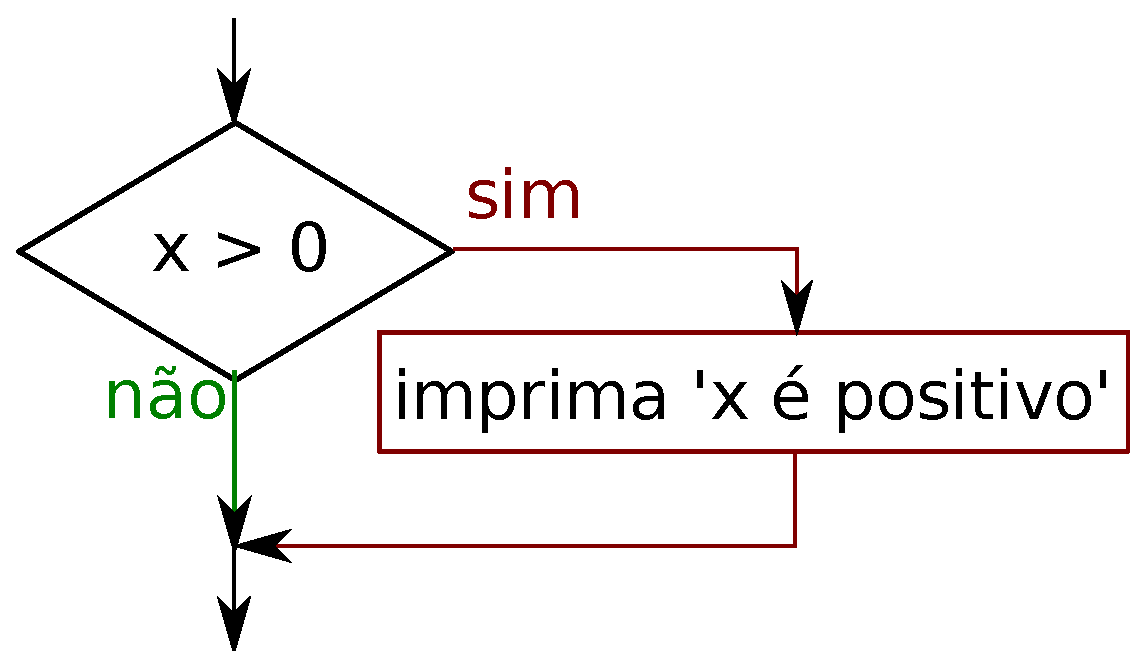
\includegraphics[height=1.75in]{figs2/if.eps}}
\afterfig

Se a condição lógica é verdadeira, então a declaração
recuada é executada. Se a condição lógica é
falsa, a declaração recuada é ignorada.

% If the logical condition is true, then the indented
% statement gets executed.  If the logical condition is 
% false, the indented statement is skipped.

\index{condição}
\index{declaração composta}
\index{declaração!composta}
% \index{condition}
% \index{compound statement}
% \index{statement!compound}

{\tt Se} declarações têm a mesma estrutura que as definições de funções
ou {\tt for} loops\footnote{Vamos aprender sobre as funções no Capítulo 4
e loops no Capítulo 5.}. A declaração é composta por uma linha de cabeçalho
que termina com o caractere dois pontos (:)
seguido por um bloco recuado. Declarações com esta são
chamado {\bf declarações compostas} porque eles estendem  
por mais de uma linha.

% {\tt if} statements have the same structure as function definitions
% or {\tt for} loops\footnote{We will learn about functions in Chapter 4
% and loops in Chapter 5.}.The statement consists of a header line
% that ends with the colon character (:) 
% followed by an indented block.  Statements like this are
% called {\bf compound statements} because they stretch 
% across more than one line.

Não há limite para o número de intruções que podem aparecer 
no corpo, mais tem de haver pelo menos um.
As vezes, é util ter um corpo sem declaraçoẽs (usualmente
como um corpo pacificador para o codigo que você não tenha escrito ate o momento). Nesse
caso, você pode usar a declaração {\tt pass}, que não faz nada.

% There is no limit on the number of statements that can appear in
% the body, but there must be at least one.
% Occasionally, it is useful to have a body with no statements (usually
% as a placekeeper for code you haven't written yet).  In that
% case, you can use the {\tt pass} statement, which does nothing.

\index{pass statement}
\index{statement!pass}

\beforeverb
\begin{verbatim}
if x < 0 :
    pass          # precisa lidar com valores negativos!
\end{verbatim}
%\begin{verbatim}
%if x < 0 :
%    pass          # need to handle negative values!
%\end{verbatim}
\afterverb
%
Se você digitar um {\tt if} no interpretador Python, o prompt vai mudar
a partir de três divisas para três pontos para indicar que você está no meio de um bloco de
declarações, como mostrado abaixo:
% If you enter an {\tt if} statement in the Python interpreter, the prompt will change 
% from three chevrons to three dots to indicate you are in the middle of a block of
% statements, as shown below:

\beforeverb
\begin{verbatim}
>>> x = 3
>>> if x < 10:
...    imprimir 'pequeno'
... 
Small
>>>
\end{verbatim}
%\begin{verbatim}
%>>> x = 3
%>>> if x < 10:
%...    print 'Small'
%... 
%Small
%>>>
%\end{verbatim}
\afterverb
%

\section{Execução alternativa}
\label{execução alternativa}
%\section{Alternative execution}
%\label{alternative execution}

\index{execução alternativa}
\index{else keyword}
\index{keyword!else}
%\index{alternative execution}
%\index{else keyword}
%\index{keyword!else}

A segunda forma do {\tt if} é a {\bf execução alternativa},
em que há duas possibilidades e a condição determina
qual é executado. A sintaxe parecida com esta:

%A second form of the {\tt if} statement is {\bf alternative execution},
%in which there are two possibilities and the condition determines
%which one gets executed.  The syntax looks like this:

\beforeverb
\begin{verbatim}
if x%2 == 0 :
    imprimir 'x ainda é'
else :
    imprimir 'x é estranho'
\end{verbatim}
%\begin{verbatim}
%if x%2 == 0 :
%    print 'x is even'
%else :
%    print 'x is odd'
%\end{verbatim}
\afterverb
%

Se o restante de {\tt x} quando dividido por 2 for 0, em seguida, nós
sabemos que {\tt x} é divisível, e o programa exibe uma mensagem para esse
efeito. Se a condição for falsa, o segundo conjunto de instruções é
executado.

%If the remainder when {\tt x} is divided by 2 is 0, then we
%know that {\tt x} is even, and the program displays a message to that
%effect.  If the condition is false, the second set of statements is
%executed.  

\beforefig
\centerline{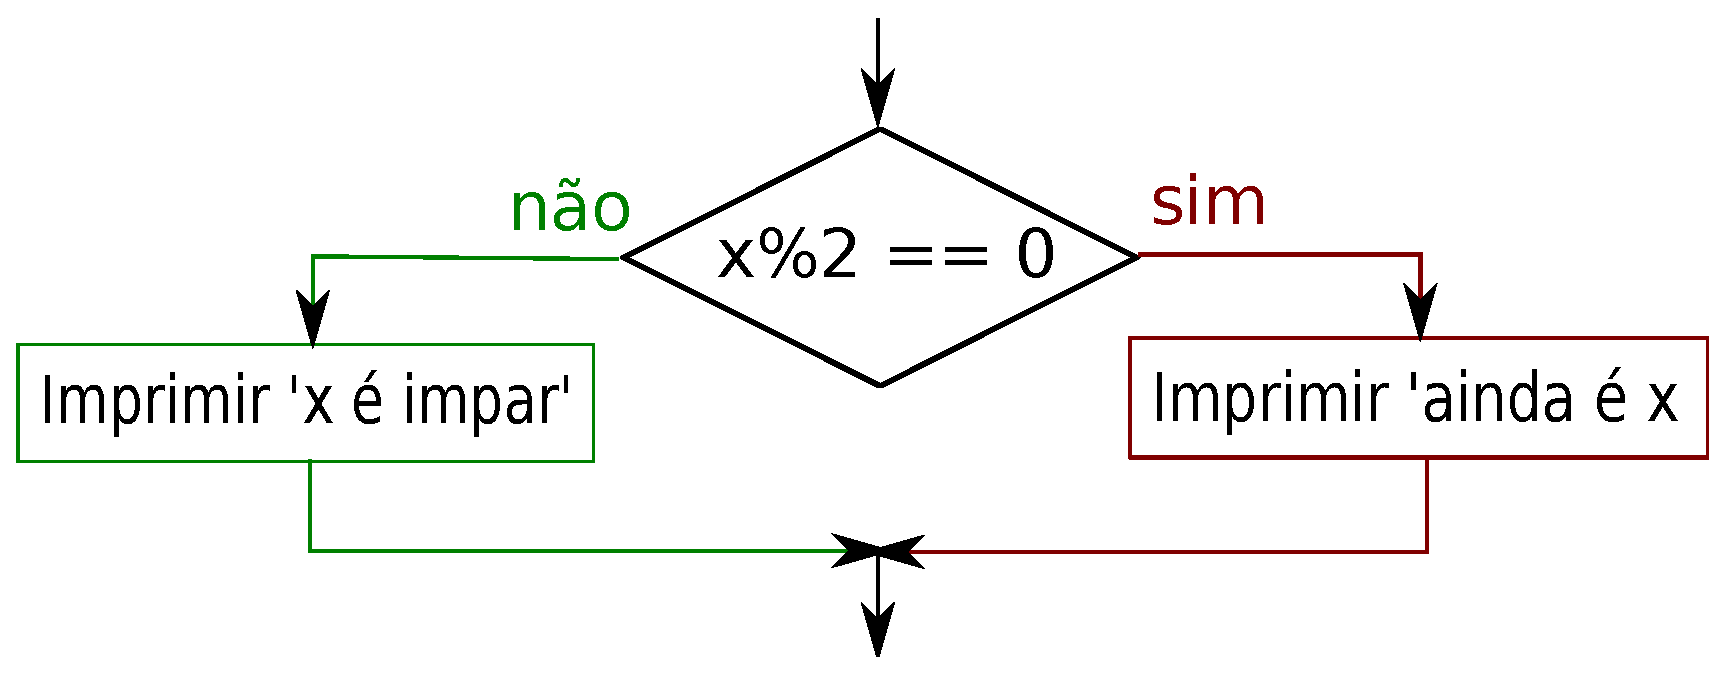
\includegraphics[height=1.75in]{figs2/if-else.eps}}
\afterfig

Uma vez que a condição deve ser verdadeira ou falsa, exatamente um das
alternativas será executada. As alternativas são chamadas de
{\bf branches}, porque eles são filiais no fluxo de execução.
%Since the condition must either be true or false, exactly one of
%the alternatives will be executed.  The alternatives are called
%{\bf branches}, because they are branches in the flow of execution.

\index{branch}



\section{Condicionais encadeadas}
%\section{Chained conditionals}
\index{chained conditional}
\index{conditional!chained}


Às vezes, há mais de duas possibilidades e precisamos de mais do que
duas condições. Uma maneira de expressar uma computação como essa é uma {\bf
chained conditional}:
%Sometimes there are more than two possibilities and we need more than
%two branches.  One way to express a computation like that is a {\bf
%chained conditional}:

\beforeverb
\begin{verbatim}
if x < y:
    imprimir 'x é menor que y'
elif x > y:
    imprimir 'x é maior que y'
else:
    imprimir 'x e y são iguais'
\end{verbatim}
\afterverb
%\begin{verbatim}
%if x < y:
%    print 'x is less than y'
%elif x > y:
%    print 'x is greater than y'
%else:
%    print 'x and y are equal'
%\end{verbatim}
\afterverb
%

{\tt elif} é uma abreviatura de `` else if. '' Mais uma vez, exatamente uma
condição será executado.
%{\tt elif} is an abbreviation of ``else if.''  Again, exactly one
%branch will be executed.  

\beforefig
\centerline{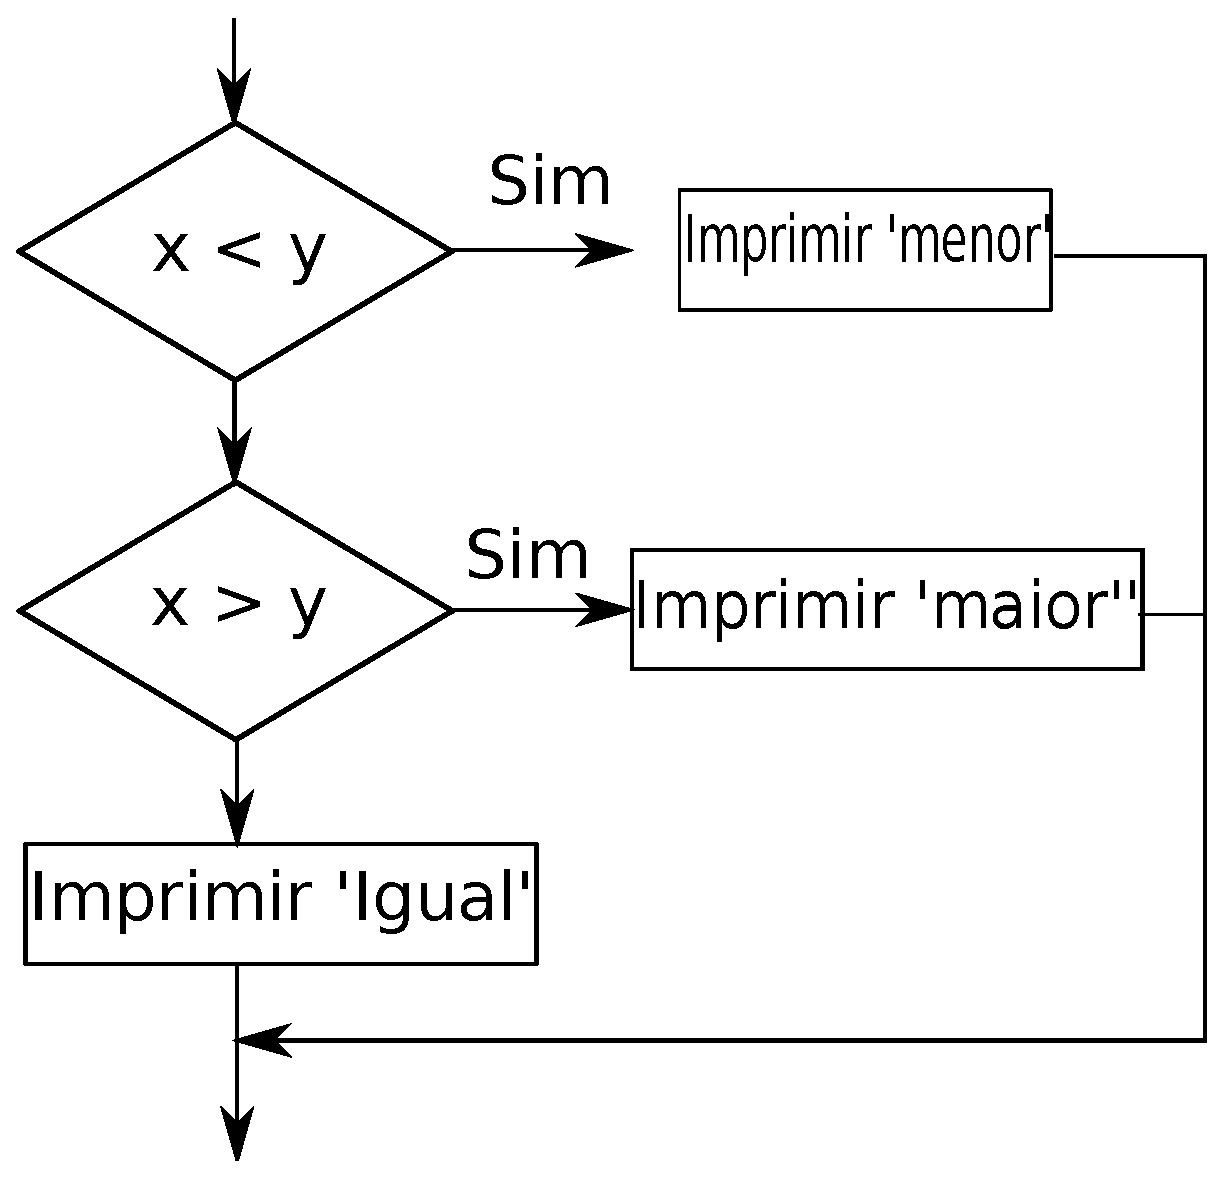
\includegraphics[height=3.00in]{figs2/elif.eps}}
\afterfig

Não há limite para o número de declarações {\tt
elif} . Se houver um cláusula {\tt else}, no final deverá
existir uma cláusula {\tt end}.

%There is no limit on the number of {\tt
%elif} statements.  If there is an {\tt else} clause, it has to be
%at the end, but there doesn't have to be one.

\index{elif keyword}
\index{keyword!elif}


\beforeverb
\begin{verbatim}
if choice == 'a':
    imprimir 'Escolha ruim'
elif choice == 'b':
    imprimir 'Boa escolha'
elif choice == 'c':
    imprimir 'Perto, mais não correto'
\end{verbatim}
%\begin{verbatim}
%if choice == 'a':
%    print 'Bad guess'
%elif choice == 'b':
%    print 'Good guess'
%elif choice == 'c':
%    print 'Close, but not correct'
%\end{verbatim}
\afterverb
%

Cada condição é verificada em ordem. Se a primeira é falsa,
a próxima será executada, e assim por diante. Se um deles é
Verdadeiro, o corresponde será executa, e a declaração
termina. Mesmo se mais do que uma condição é verdadeira, apenas o
primeiro verdadeiro é executado.

%Each condition is checked in order.  If the first is false,
%the next is checked, and so on.  If one of them is
%true, the corresponding branch executes, and the statement
%ends.  Even if more than one condition is true, only the
%first true branch executes.  



\section{Condicionais aninhados}
%\section{Nested conditionals}
\index{nested conditional}
\index{conditional!nested}

Uma condição também pode ser aninhado em outro. Nós poderíamos ter
escrito o exemplo de três ramificações como esta:

%One conditional can also be nested within another.  We could have
%written the three-branch example like this:

\beforeverb
\begin{verbatim}
if x == y:
    imprimir 'x e y são iguais'
else:
    if x < y:
        imprimir 'x é menor que y'
    else:
        imprimir 'x é maior que y'
\end{verbatim}
%\begin{verbatim}
%if x == y:
%    print 'x and y are equal'
%else:
%    if x < y:
%        print 'x is less than y'
%    else:
%        print 'x is greater than y'
%\end{verbatim}
\afterverb
%
A condicional externa contém duas ramificações. A
primeiro ramificação contém uma instrução simples. A segundo ramificação
contém outra declaração {\tt if}, que tem duas ramificações
próprias. Esses duas ramifiações são ambas instruções simples,
embora pudessem ter sido instruções condicionais também.

%The outer conditional contains two branches.  The
%first branch contains a simple statement.  The second branch
%contains another {\tt if} statement, which has two branches of its
%own.  Those two branches are both simple statements,
%although they could have been conditional statements as well.

\beforefig
\centerline{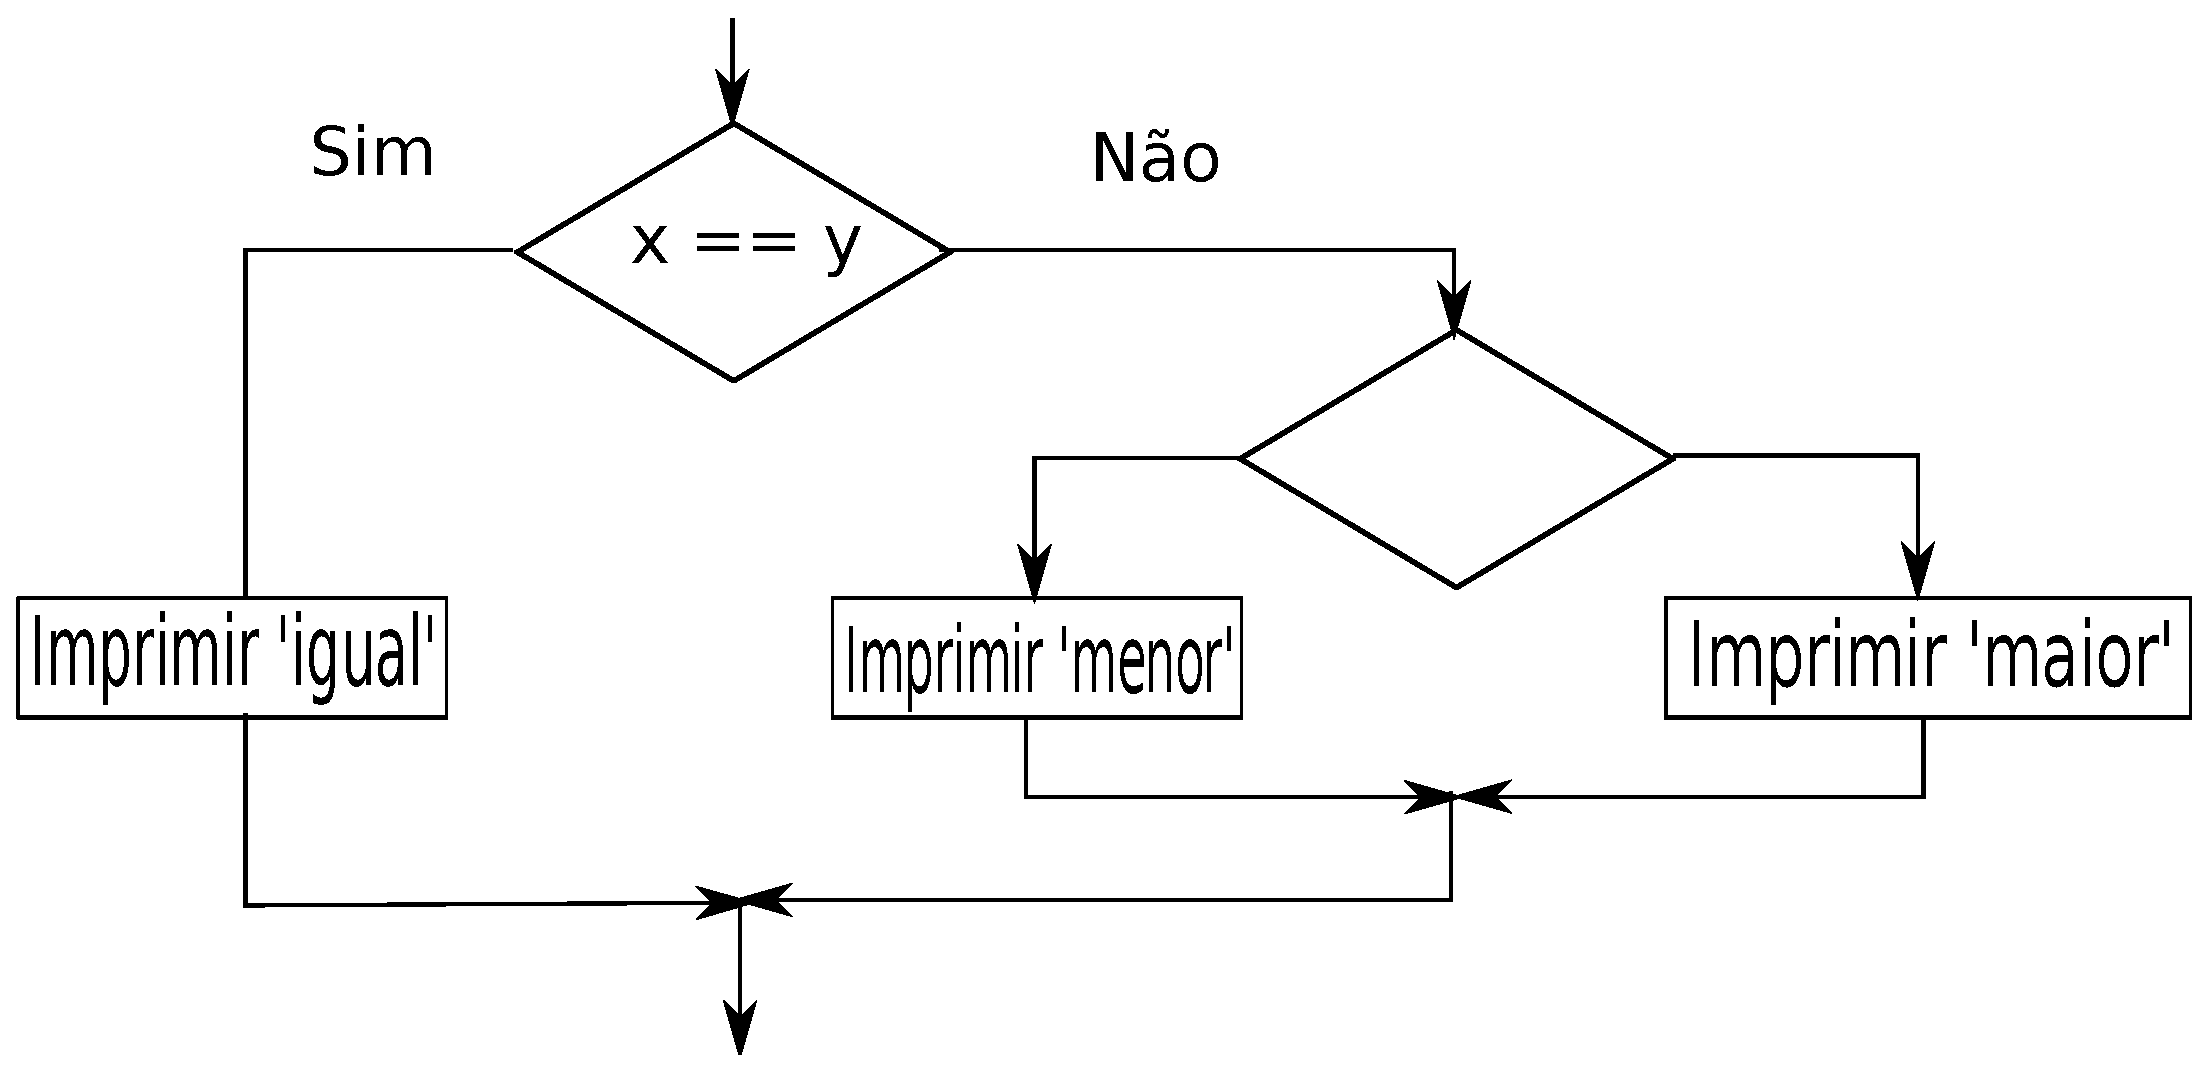
\includegraphics[height=2.50in]{figs2/nested.eps}}
\afterfig


Embora a identação das instruções torna a estrutura
visível, {\bf condicionais aninhadas} fica difícil de ler muito
rapidamente. Em geral, é uma boa idéia sempre que possível evitá-las quando puder.

%Although the indentation of the statements makes the structure
%apparent, {\bf nested conditionals} become difficult to read very
%quickly. In general, it is a good idea to avoid them when you can.


Os operadores lógicos muitas vezes fornecem uma maneira de simplificar as declarações de condições
aninhadas. Por exemplo, podemos reescrever o código a seguir usando um
condicional único:

%Logical operators often provide a way to simplify nested conditional
%statements.  For example, we can rewrite the following code using a
%single conditional:

\beforeverb
\begin{verbatim}
if 0 < x:
    if x < 10:
        imprimir 'x é um número positivo de um dígito.'
\end{verbatim}
%\begin{verbatim}
%if 0 < x:
%    if x < 10:
%        print 'x is a positive single-digit number.'
%\end{verbatim}
%\afterverb
%
A instrução {\tt imprimir} é executada somente se ambas as condições forem 
verdadeiras, para que possamos obter o mesmo efeito com o operador {\tt and}:

%The {\tt print} statement is executed only if we make it past both
%conditionals, so we can get the same effect with the {\tt and} operator:

\beforeverb
\begin{verbatim}
if 0 < x and x < 10:
    imprimir 'x é um número positivo de um dígito.'
\end{verbatim}
%\begin{verbatim}
%if 0 < x and x < 10:
%    print 'x is a positive single-digit number.'
%\end{verbatim}
\afterverb

\section{Catching exceções usando try e except}
%\section{Catching exceptions using try and except}
\label{catch1}

Anteriormente, vimos um segmento de código onde foi utilizado o 
\verbo"raw_input" e {\tt int} funções para ler e analisar um 
número inteiro informado pelo usuário. 
Também vimos como pode ser traiçoeiro utilizar isso:

%Earlier we saw a code segment where we used the \verb"raw_input" and
%{\tt int} functions to read and parse an integer number entered by
%the user.  We also saw how treacherous doing this could be:

\beforeverb
\begin{verbatim}
>>> Velocidade = raw_input (prompt)
O que ... é a velocidade da velocidade aerodinâmica de uma andorinha unladen?
O que quer dizer, um Africano ou uma andorinha Europeia?
>>> Int (velocidade)
ValueError: inválido literal para int ()
>>>
\end{verbatim}
\afterverb
%\begin{verbatim}
%>>> speed = raw_input(prompt)
%What...is the airspeed velocity of an unladen swallow?
%What do you mean, an African or a European swallow?
%>>> int(speed)
%ValueError: invalid literal for int()
%>>>
%\end{verbatim}
%
Quando estamos executando estas declarações no interpretador Python,
temos um novo prompt do intérprete, acho que ``oops'', e nos movemos
para o nosso próximo comunicado.

%When we are executing these statements in the Python interpreter, 
%we get a new prompt from the interpreter, think ``oops'', and move 
%on to our next statement.  

No entanto, se você colocar esse código em um
script Python e este erro ocorre, o script imediatamente
pára em suas faixas com um rastreamento.
Não executa a seguinte instrução.

%However if you place this code in a 
%Python script and this error occurs, your script immediately 
%stops in its tracks with a traceback.  
%It does not execute the following statement. 
\index{traceback}


Aqui está um programa de exemplo para converter uma temperatura Fahrenheit
a uma temperatura em graus Celsius:

%Here is a sample program to convert a Fahrenheit temperature 
%to a Celsius temperature:
\index{fahrenheit}
\index{celsius}
\index{temperature conversion}

\beforeverb
\begin{verbatim}
inp = raw_input('Digite a Temperatura Fahrenheit:')
fahr = float(inp)
cel = (fahr - 32.0) * 5.0 / 9.0
print cel
\end{verbatim}
%\begin{verbatim}
%inp = raw_input('Enter Fahrenheit Temperature:')
%fahr = float(inp)
%cel = (fahr - 32.0) * 5.0 / 9.0
%print cel
%\end{verbatim}
\afterverb
%

Se executar esse código e informar uma entrada inválida, ele simplesmente falha
com uma mensagem de erro hostil:

%If we execute this code and give it invalid input, it simply fails
%with an unfriendly error message:

\beforeverb
\begin{verbatim}
python fahren.py 
Digite a Temperatura Fahrenheit:72
22.2222222222

python fahren.py 
Digite a Temperatura Fahrenheit:fred
Traceback (chamada mais recente passada):
  File "fahren.py", line 2, in <module>
    fahr = float(inp)
ValueError: invalid literal for float(): fred
\end{verbatim}
%\begin{verbatim}
%python fahren.py 
%Enter Fahrenheit Temperature:72
%22.2222222222

%python fahren.py 
%Enter Fahrenheit Temperature:fred
%Traceback (most recent call last):
%  File "fahren.py", line 2, in <module>
%    fahr = float(inp)
%ValueError: invalid literal for float(): fred
%\end{verbatim}
\afterverb
%

Existe uma estrutura de execução condicional incorporado
Python para lidar com esses tipos esperados e inesperados de
erros chamados ``try / except''. A ideia de {\tt try}
e {\tt except} é que você sabe que alguma sequência
de instrução pode ter algum problema e você quer
adicionar um pouco de instruções a serem executadas se ocorrer um erro.
Estas declarações adicionais (os blocos except) são ignoradas
se não há erro.

%There is a conditional execution structure built into 
%Python to handle these types of expected and unexpected
%errors called ``try / except''.  The idea of {\tt try}
%and {\tt except} is that you know that some sequence
%of instruction(s) may have a problem and you want to 
%add some statements to be executed if an error occurs.
%These extra statements (the except block) are ignored
%if there is no error.

Você pode pensar nos recursos {\tt try} e {\tt except}
em Python como uma ``política segura'' em uma seqüência de
declarações.

%You can think of the {\tt try} and {\tt except} feature
%in Python as an ``insurance policy'' on a sequence of
%statements.

Podemos reescrever nosso conversor de temperatura da seguinte forma:
%We can rewrite our temperature converter as follows:

\beforeverb
\begin{verbatim}
inp = raw_input('Digite a Temperatura Fahrenheit:')
try:
    fahr = float(inp)
    cel = (fahr - 32.0) * 5.0 / 9.0
    print cel
except:
    print 'Por favor, digite um numero'
\end{verbatim}
\afterverb
%

Python começa executando a
sequência de declarações no
bloco {\tt try}. Se tudo correr
bem, ele ignora o bloco {\tt except} e prossegue. Se uma
exceção ocorre no bloco {\tt try},
o Python pula para fora do bloco {\tt try}  e
executa a sequência de declarações do bloco {\tt except}.

%Python starts by executing the 
%sequence of statements in the 
%{\tt try} block.  If all goes
%well, it skips the {\tt except} block and proceeds.  If an
%exception occurs in the {\tt try} block, 
%Python jumps out of the {\tt try} block and
%xecutes the sequence of statements in the {\tt except} block.

\beforeverb
\begin{verbatim}
python fahren2.py 
Digite a Temperatura Fahrenheit:72
22.2222222222

python fahren2.py 
Digite a Temperatura Fahrenheit:fred
Por favor, digite um numero
\end{verbatim}
\afterverb
%


Manipulação de uma exceção com uma declaração {\tt try} é chamado uma exceção {\bf
catching}. Neste exemplo, a cláusula {\tt except} imprime uma mensagem de erro. Em geral,
capturar uma exceção dá-lhe a oportunidade de corrigir o problema, ou tentar
mais uma vez, ou pelo menos terminar o programa sem erros não tratáveis.

%Handling an exception with a {\tt try} statement is called {\bf
%catching} an exception.  In this example, the {\tt except} clause
%prints an error message.  In general,
%catching an exception gives you a chance to fix the problem, or try
%again, or at least end the program gracefully.

\section{Short-circuit avaliação de expressões lógicas}
%\section{Short-circuit evaluation of logical expressions}
\index{short circuit}


Quando Python está processando uma expressão lógica, como
{\tt x >= 2 e (x / y)> 2}, ele avalia a expressão
da esquerda para a direita. Devido à definição do {\tt and},
Se {\tt x} é inferior a 2, a expressão {\tt x >= 2} é
{\tt False} e assim por toda a expressão é {\tt False} independentemente
de saber se {\tt (x/y) > 2} avaliada como {\tt True} ou {\tt False}.

%When Python is processing a logical expression such as 
%{\tt x >= 2 and (x/y) > 2}, it evaluates the expression
%from left to right.  Because of the definition of {\tt and},
%if {\tt x} is less than 2, the expression {\tt x >= 2} is 
%{\tt False} and so the whole expression is {\tt False} regardless
%of whether {\tt (x/y) > 2} evaluates to {\tt True} or {\tt False}.

Quando Python detecta que não há nada a ser adquirida através da avaliação do 
resto de uma expressão lógica, ele para a sua avaliação e não 
faz os cálculos no resto da expressão lógica.
Quando a avaliação de uma expressão lógica para porque o valor global já 
é conhecido, a avaliãção é chamada de {\bf short-circuiting}.

%When Python detects that there is nothing to be gained by evaluating
%the rest of a logical expression, it stops its evaluation and does
%not do the computations in the rest of the logical expression.  
%When the evaluation of a logical expression stops because the overall
%value is already known, it is called {\bf short-circuiting} 
%the evaluation.

\index{guardian pattern}
\index{pattern!guardian}

Embora isso possa parecer uma ponta fina, o comportamento de short-circuit
leva a uma técnica inteligente chamado {\bf guardian pattern}.
Considere a seguinte sequência de código no interpretador Python:
%While this may seem like a fine point, the short-circuit behavior
%leads to a clever technique called the {\bf guardian pattern}.  
%Consider the following code sequence in the Python interpreter:

\beforeverb
\begin{verbatim}
>>> x = 6 
>>> y = 2
>>> x >= 2 and (x/y) > 2
True
>>> x = 1 
>>> y = 0
>>> x >= 2 and (x/y) > 2
False
>>> x = 6
>>> y = 0
>>> x >= 2 and (x/y) > 2
Traceback (chamada mais recente passada):
  File "<stdin>", line 1, in <module>
ZeroDivisionError: divisão inteira ou modulo por zero
>>> 
\end{verbatim}
%\begin{verbatim}
%>>> x = 6 
%>>> y = 2
%>>> x >= 2 and (x/y) > 2
%True
%>>> x = 1 
%>>> y = 0
%>>> x >= 2 and (x/y) > 2
%False
%>>> x = 6
%>>> y = 0
%>>> x >= 2 and (x/y) > 2
%Traceback (most recent call last):
%  File "<stdin>", line 1, in <module>
%ZeroDivisionError: integer division or modulo by zero
%>>> 
%\end{verbatim}
\afterverb
%
O terceiro cálculo falhou porque Python estava avaliando {\tt (x/y)}
e {\tt y} foi zero, o que faz com que gere um erro de execução. Mas o segundo exemplo
\emph{não} falham porque a primeira parte da expressão {\tt x >= 2} é
avaliada como {\tt False} para o {\tt (x/y)} não foi já realizada
devido à regra {\bf short-circuit} e não houve erro.

%The third calculation failed because Python was evaluating {\tt (x/y)}
%and {\tt y} was zero, which causes a runtime error.  But the second example
%did \emph{not} fail because the first part of the expression {\tt x >= 2} 
%evaluated to {\tt False} so the {\tt (x/y)} was not ever executed 
%due to the {\bf short-circuit} rule and there was no error.


Podemos construir a expressão lógica para colocar estrategicamente a avaliação {\bf guard}
pouco antes da avaliação que pode causar um erro da seguinte forma:

%We can construct the logical expression to strategically place a {\bf guard}
%evaluation just before the evaluation that might cause an error as follows:

\beforeverb
\begin{verbatim}
>>> x = 1
>>> y = 0
>>> x >= 2 and y != 0 and (x/y) > 2
False
>>> x = 6 
>>> y = 0
>>> x >= 2 and y != 0 and (x/y) > 2
False
>>> x >= 2 and (x/y) > 2 and y != 0
Traceback (chamada mais recente passada):
  File "<stdin>", line 1, in <module>
ZeroDivisionError: divisão inteira ou modulo por zero
>>>
\end{verbatim}
%\begin{verbatim}
%>>> x = 1
%>>> y = 0
%>>> x >= 2 and y != 0 and (x/y) > 2
%False
%>>> x = 6 
%>>> y = 0
%>>> x >= 2 and y != 0 and (x/y) > 2
%False
%>>> x >= 2 and (x/y) > 2 and y != 0
%Traceback (most recent call last):
%  File "<stdin>", line 1, in <module>
%ZeroDivisionError: integer division or modulo by zero
%>>>
%\end{verbatim}
\afterverb
%

Na primeira expressão lógica, {\tt x >= 2} é \tt False} para a avaliação
parar no {\tt and}. Na segunda expressão lógica, {\tt x >= 2} é {\tt True}
mas {\tt y != 0} é {\tt False} para que nunca ocorra {\tt (x/y)}.

%In the first logical expression, {\tt x >= 2} is {\tt False} so the evaluation
%stops at the {\tt and}.  In the second logical expression, {\tt x >= 2} is {\tt True}
%but {\tt y != 0} is {\tt False} so we never reach {\tt (x/y)}.


Na terceira expressão lógica, o {\tt y != 0} é \emph{depois} do Cálculo
{\tt (x/y) } de modo que a  expressão termina com um erro.

%In the third logical expression, the {\tt y != 0} is \emph{after} the 
%{\tt (x/y) } calculation so the expression fails with an error.


Na segunda expressão, dizemos que {\tt y != 0} atua como um {\bf guard}
para garantir que só executamos {{\tt (x/y)} se {\tt y} é diferente de zero.

%In the second expression, we say that {\tt y != 0} acts as a {\bf guard}
%to insure that we only execute {\tt (x/y)} if {\tt y} is non-zero.


\section{Depuração}
%\section{Debugging}
\label{whitespace}
\index{debugging}
\index{traceback}

O Python traceback é exibido quando ocorre um erro, e contém
várias informações, mas pode ser esmagadora. A maioria
das informações são úteis geralmente:

%The traceback Python displays when an error occurs contains
%a lot of information, but it can be overwhelming.  The most
%useful parts are usually:

\begin{itemize}

\item Que tipo de erro que era, e

\item Onde ocorreu.

\end{itemize}
%\begin{itemize}

%\item What kind of error it was, and

%\item Where it occurred.

%\end{itemize}

Os erros de sintaxe são geralmente fáceis de encontrar, mas há algumas
pegadinhas. erros de espaço em branco que podem ser difíceis, porque os espaços e
guias são invisíveis e que são utilizados para ignorá-los.

%Syntax errors are usually easy to find, but there are a few
%gotchas.  Whitespace errors can be tricky because spaces and
%tabs are invisible and we are used to ignoring them.

\index{whitespace}

\beforeverb
\begin{verbatim}
>>> x = 5
>>>  y = 6
  File "<stdin>", line 1
    y = 6
    ^
SyntaxError: Syntax inválida
\end{verbatim}
%\begin{verbatim}
%>>> x = 5
%>>>  y = 6
%  File "<stdin>", line 1
%    y = 6
%    ^
%SyntaxError: invalid syntax
%\end{verbatim}
\afterverb
%
Neste exemplo, o problema é que a segunda linha é indentada por
um espaço. Mas a mensagem de erro aponta para {\tt y}, que é
enganosa. Em geral, as mensagens de erro indicam onde o problema foi
descoberto, mas o erro real pode estar no início do código,
às vezes em uma linha anterior.

%In this example, the problem is that the second line is indented by
%one space.  But the error message points to {\tt y}, which is
%misleading.  In general, error messages indicate where the problem was
%discovered, but the actual error might be earlier in the code,
%sometimes on a previous line.

\index{error!runtime}
\index{runtime error}

O mesmo ocorre para erros de execução. Suponha que você está tentando
calcular uma relação sinal-ruído em decibéis. A fórmula
é $SNR_{db} = 10 \log_{10} (P_{signal} / P_{noise})$. Em Python,
você pode escrever algo como isto:

%The same is true of runtime errors.  Suppose you are trying
%to compute a signal-to-noise ratio in decibels.  The formula
%is $SNR_{db} = 10 \log_{10} (P_{signal} / P_{noise})$.  In Python,
%you might write something like this:

\beforeverb
\begin{verbatim}
import math
signal_power = 9
noise_power = 10
ratio = signal_power / noise_power
decibels = 10 * math.log10(ratio)
print decibels
\end{verbatim}
\afterverb
%
Mas quando você executá-lo, você recebe uma mensagem de erro \footnote{Em Python 3.0,
   você não receber uma mensagem de erro; o operador executa a
   divisão, mesmo com operador inteiro de ponto flutuante}.:

%But when you run it, you get an error message\footnote{In Python 3.0,
%  you no longer get an error message; the division operator performs
%  floating-point division even with integer operands.}:

\index{exception!OverflowError}
\index{OverflowError}

\beforeverb
\begin{verbatim}
Traceback (chamada mais recente passada):
  File "snr.py", line 5, in ?
    decibels = 10 * math.log10(ratio)
OverflowError: erro gama de matemática
\end{verbatim}
%\begin{verbatim}
%Traceback (most recent call last):
%  File "snr.py", line 5, in ?
%    decibels = 10 * math.log10(ratio)
%OverflowError: math range error
%\end{verbatim}
\afterverb
%

A mensagem de erro indica que é a linha 5, mas não há nada
errado com essa linha. Para encontrar o verdadeiro erro, pode ser
útil imprimir o valor de {\tt rateio}, o que acaba 
sendo 0. O problema é na linha 4, porque dividir dois inteiros
causa ``floor division''''. A solução é para representar a potência do sinal
e potência de ruído com valores de ponto flutuante.

%The error message indicates line 5, but there is nothing
%wrong with that line.  To find the real error, it might be
%useful to print the value of {\tt ratio}, which turns out to
%be 0.  The problem is in line 4, because dividing two integers
%does floor division.  The solution is to represent signal power
%and noise power with floating-point values.

\index{floor division}
\index{division!floor}

Em geral, as mensagens de erro dizem onde o problema foi descoberto,
mas isso não é muitas vezes onde ele foi causado.

%In general, error messages tell you where the problem was discovered, 
%but that is often not where it was caused.


\section{Glossário}
%\section{Glossary}

\begin{description}


\item[body:] A sequência de declarações dentro de uma instrução composta
%\item[body:] The sequence of statements within a compound statement.
\index{body}

\item[boolean expression:] Uma expressão cujo valor é
%\item[boolean expression:]  An expression whose value is either 
{\tt True} or {\tt False}.
\index{boolean expression}
\index{expression!boolean}

\item[branch:] Uma das seqüências alternativas de declarações em uma 
instrução condicional.
%\item[branch:] One of the alternative sequences of statements in
%a conditional statement.
\index{branch}

\item[chained conditional:]  A instrução condicional com uma série 
de ramificações alternativas.
%\item[chained conditional:]  A conditional statement with a series
%of alternative branches.
\index{chained conditional}
\index{conditional!chained}

\item[comparison operator:] Um dos operadores que compara 
seus operandos: {\tt ==}, {\tt !=}, {\tt >}, {\tt <}, {\tt >=}, and {\tt <=}.
%\item[comparison operator:] One of the operators that compares
%its operands: {\tt ==}, {\tt !=}, {\tt >}, {\tt <}, {\tt >=}, and {\tt <=}.

\item[conditional statement:] Uma declaração que controla o fluxo de 
execução dependendo de alguma condição
%\item[conditional statement:]  A statement that controls the flow of
%execution depending on some condition.
\index{conditional statement}
\index{statement!conditional}

\item[condition:] A expressão booleana em uma declaração condicional 
que determina qual a condição é executado.
%\item[condition:] The boolean expression in a conditional statement
%that determines which branch is executed.
\index{condition}

\item[compound statement:]  Uma declaração de que consiste em um cabeçalho 
e um corpo. O cabeçalho termina com dois pontos (:). O corpo é recuado em 
relação ao cabeçalho.
%\item[compound statement:]  A statement that consists of a header
%and a body.  The header ends with a colon (:).  The body is indented
%relative to the header.
\index{compound statement}

\item[guardian pattern:] 
Onde nós construimos uma expressão lógica com 
comparações adicionais para 
aproveitar o comportamento de short-circuit.
%\item[guardian pattern:] Where we construct a logical expression 
%with additional
%comparisons to take advantage of the short-circuit behavior.
\index{guardian pattern}
\index{pattern!guardian}

\item[logical operator:] Um dos operadores que combina expressões 
booleanas: {\tt and}, {\tt or}, and {\tt not}.
%\item[logical operator:] One of the operators that combines boolean
%expressions: {\tt and}, {\tt or}, and {\tt not}.

\item[nested conditional:]  A instrução condicional que aparece em um dos 
ramos de uma outra instrução condicional.
%\item[nested conditional:]  A conditional statement that appears
%in one of the branches of another conditional statement.
\index{nested conditional}
\index{conditional!nested}

\item[traceback:]  A lista das funções que estão em execução, 
impressa quando ocorre uma exceção.
%\item[traceback:]  A list of the functions that are executing,
%printed when an exception occurs.
\index{traceback}

\item[short circuit:] Quando Python é a meio de avaliação de uma expressão 
lógica e para a avaliação porque Python 
sabe o valor final para a expressão
sem a necessidade de avaliar o resto da expressão.
%\item[short circuit:]  When Python is part-way through evaluating a 
%logical expression and stops the evaluation because Python 
%knows the final value for the expression 
%without needing to evaluate the rest of the expression.
\index{short circuit}

\end{description}

\section{Exercícios}
%\section{Exercises}

\begin{ex}
Reescrever o seu cálculo de pagamento para dar ao trabalhador 1.5
vezes a taxa horária para
horas trabalhadas acima de 40 horas.
%Rewrite your pay computation to give the employee 1.5 
%times the hourly rate for 
%hours worked above 40 hours.

\begin{verbatim}
Digite as Horas: 45
Digite a Taxa: 10
Pagamento: 475.0
\end{verbatim}
\end{ex}
%\begin{verbatim}
%Enter Hours: 45
%Enter Rate: 10
%Pay: 475.0
%\end{verbatim}
%\end{ex}

\begin{ex}
Reescrever seu programa de pagamento usando {\tt try} e {\tt except} 
para que o programa lida com entrada não numérica amigavelmente
imprimindo uma mensagem e sair do programa.
A seguir mostra duas execuções do programa:
%Rewrite your pay program using {\tt try} and {\tt except} 
%so that your program handles non-numeric input gracefully
%by printing a message and exiting the program.
%The following shows two executions of the program:

\begin{verbatim}
Digite as Horas: 20
Digite a Taxa: nine
Erro, por favor, informe entrada numérica

Digite as Horas: forty
Erro, por favor, informe entrada numérica
\end{verbatim}
\end{ex}
%\begin{verbatim}
%Enter Hours: 20
%Enter Rate: nine
%Error, please enter numeric input

%Enter Hours: forty
%Error, please enter numeric input
%\end{verbatim}
%\end{ex}

\begin{ex}
Escreva um programa para solicitar uma pontuação entre 0,0 e 1,0.
Se o resultado estiver fora da faixa, imprimir uma mensagem de erro. Se a pontuação
está entre 0,0 e 1,0, imprimir um grau utilizando a seguinte 
tabela:
%Write a program to prompt for a score between 0.0 and 1.0.
%If the score is out of range, print an error message.  If the score
%is between 0.0 and 1.0, print a grade using the following 
%table:

\begin{verbatim}
Ponto   Grau
>= 0.9   A
>= 0.8   B
>= 0.7   C
>= 0.6   D
< 0.6    F

Digite a Pontuação: 0.95
A

Digite a Pontuação: perfect
Bad score

Digite a Pontuação: 10.0
Bad score

Digite a Pontuação: 0.75
C

Digite a Pontuação: 0.5
F
\end{verbatim}
%\begin{verbatim}
%Score   Grade
%>= 0.9     A
%>= 0.8     B
%>= 0.7     C
%>= 0.6     D
%< 0.6    F

%Enter score: 0.95
%A

%Enter score: perfect
%Bad score

%Enter score: 10.0
%Bad score

%Enter score: 0.75
%C

%Enter score: 0.5
%F
%\end{verbatim}

Executar o programa repetidamente, como mostrado acima, para testar os 
diversos valores diferentes para a entrada.
%Run the program repeatedly as shown above to test the 
%various different values for input.
\end{ex}



% TODO % LaTeX source for ``Python for Informatics: Exploring Information''
% Copyright (c)  2010-  Charles R. Severance, All Rights Reserved

\chapter{Functions}
\label{funcchap}

\section{Function calls}
\label{functionchap}
\index{function call}

In the context of programming, a {\bf function} is a named sequence of
statements that performs a computation.  When you define a function,
you specify the name and the sequence of statements.  Later, you can
``call'' the function by name.  
We have already seen one example of a {\bf function call}:

\beforeverb
\begin{verbatim}
>>> type(32)
<type 'int'>
\end{verbatim}
\afterverb
%
The name of the function is {\tt type}.  The expression in parentheses
is called the {\bf argument} of the function.  The argument is 
a value or variable that we are passing into the function as input 
to the function.  
The result, for the {\tt type} function, is the type of the argument.

\index{parentheses!argument in}

It is common to say that a function ``takes'' an argument and ``returns''
a result.  The result is called the {\bf return value}.

\index{argument}
\index{return value}

\section{Built-in functions}

Python provides a number of important built-in functions that
we can use without needing to provide the function definition.
The creators of Python wrote a set of functions 
to solve common problems and included them in Python for us to use.

The {\tt max} and {\tt min} functions give us the largest and 
smallest values in a list, respectively:

\beforeverb
\begin{verbatim}
>>> max('Hello world')
'w'
>>> min('Hello world')
' '
>>>
\end{verbatim}
\afterverb
%
The {\tt max} function tells us the ``largest character'' in the 
string (which turns out to be the letter ``w'') and the {\tt min}
function shows us the smallest character (which turns out to be a 
space).

Another very common built-in function is the {\tt len} function
which tells us how many items are in its argument. If the argument
to {\tt len} is a string, it returns the number of characters 
in the string.

\beforeverb
\begin{verbatim}
>>> len('Hello world')
11
>>>
\end{verbatim}
\afterverb
%
These functions are not limited to looking at strings. They can operate
on any set of values, as we will see in later chapters.

You should treat the names of built-in functions as reserved words (i.e.,
avoid using ``max'' as a variable name).

\section{Type conversion functions}
\index{conversion!type}
\index{type conversion}

% from Elkner:
% comment on whether these things are _really_ functions?
% use max as an example of a built-in?

% my reply:
% they are on the list of ``built-in functions'' so I am
% willing to call them functions.

Python also provides built-in functions that convert values
from one type to another.  The {\tt int} function takes any value and
converts it to an integer, if it can, or complains otherwise:

\index{int function}
\index{function!int}

\beforeverb
\begin{verbatim}
>>> int('32')
32
>>> int('Hello')
ValueError: invalid literal for int(): Hello
\end{verbatim}
\afterverb
%
{\tt int} can convert floating-point values to integers, but it
doesn't round off; it chops off the fraction part:

\beforeverb
\begin{verbatim}
>>> int(3.99999)
3
>>> int(-2.3)
-2
\end{verbatim}
\afterverb
%
{\tt float} converts integers and strings to floating-point
numbers:

\index{float function}
\index{function!float}

\beforeverb
\begin{verbatim}
>>> float(32)
32.0
>>> float('3.14159')
3.14159
\end{verbatim}
\afterverb
%
Finally, {\tt str} converts its argument to a string:

\index{str function}
\index{function!str}

\beforeverb
\begin{verbatim}
>>> str(32)
'32'
>>> str(3.14159)
'3.14159'
\end{verbatim}
\afterverb
%

\section{Random numbers}

\index{random number}
\index{number, random}
\index{deterministic}
\index{pseudorandom}

Given the same inputs, most computer programs generate the same
outputs every time, so they are said to be {\bf deterministic}.
Determinism is usually a good thing, since we expect the same
calculation to yield the same result.  For some applications, though,
we want the computer to be unpredictable.  Games are an obvious
example, but there are more.

Making a program truly nondeterministic turns out to be not so easy,
but there are ways to make it at least seem nondeterministic.  One of
them is to use {\bf algorithms} that generate {\bf pseudorandom} numbers.
Pseudorandom numbers are not truly random because they are generated
by a deterministic computation, but just by looking at the numbers it
is all but impossible to distinguish them from random.

\index{random module}
\index{module!random}

The {\tt random} module provides functions that generate
pseudorandom numbers (which I will simply call ``random'' from
here on).

\index{random function}
\index{function!random}

The function {\tt random} returns a random float
between 0.0 and 1.0 (including 0.0 but not 1.0).  Each time you
call {\tt random}, you get the next number in a long series.  To see a
sample, run this loop:

\beforeverb
\begin{verbatim}
import random

for i in range(10):
    x = random.random()
    print x
\end{verbatim}
\afterverb
%
This program produces the following list of 10 random numbers
between 0.0 and up to but not including 1.0.

\beforeverb
\begin{verbatim}
0.301927091705
0.513787075867
0.319470430881
0.285145917252
0.839069045123
0.322027080731
0.550722110248
0.366591677812
0.396981483964
0.838116437404
\end{verbatim}
\afterverb
%
\begin{ex}
Run the program on your system and see what numbers you get.
Run the program more than once and see what numbers you get.
\end{ex}

The {\tt random} function is only one of many 
functions that handle random numbers.
The function {\tt randint} takes the parameters {\tt low} and
{\tt high}, and returns an integer between {\tt low} and
{\tt high} (including both).

\index{randint function}
\index{function!randint}

\beforeverb
\begin{verbatim}
>>> random.randint(5, 10)
5
>>> random.randint(5, 10)
9
\end{verbatim}
\afterverb
%
To choose an element from a sequence at random, you can use
{\tt choice}:

\index{choice function}
\index{function!choice}

\beforeverb
\begin{verbatim}
>>> t = [1, 2, 3]
>>> random.choice(t)
2
>>> random.choice(t)
3
\end{verbatim}
\afterverb
%
The {\tt random} module also provides functions to generate
random values from continuous distributions including
Gaussian, exponential, gamma, and a few more.

\section{Math functions}
\index{math function}
\index{function, math}
\index{module}
\index{module object}

Python has a {\tt math} module that provides most of the familiar
mathematical functions.  
Before we can use the module, we have to import it:

\beforeverb
\begin{verbatim}
>>> import math
\end{verbatim}
\afterverb
%
This statement creates a {\bf module object} named math.  If
you print the module object, you get some information about it:

\beforeverb
\begin{verbatim}
>>> print math
<module 'math' from '/usr/lib/python2.5/lib-dynload/math.so'>
\end{verbatim}
\afterverb
%
The module object contains the functions and variables defined in the
module.  To access one of the functions, you have to specify the name
of the module and the name of the function, separated by a dot (also
known as a period).  This format is called {\bf dot notation}.

\index{dot notation}

\beforeverb
\begin{verbatim}
>>> ratio = signal_power / noise_power
>>> decibels = 10 * math.log10(ratio)

>>> radians = 0.7
>>> height = math.sin(radians)
\end{verbatim}
\afterverb
%
The first example computes the logarithm base 10 of the
signal-to-noise ratio.  The math module also provides a
function called {\tt log} that computes logarithms base {\tt e}.

\index{log function}
\index{function!log}
\index{sine function}
\index{radian}
\index{trigonometric function}
\index{function, trigonometric}

The second example finds the sine of {\tt radians}.  The name of the
variable is a hint that {\tt sin} and the other trigonometric
functions ({\tt cos}, {\tt tan}, etc.)  take arguments in radians. To
convert from degrees to radians, divide by 360 and multiply by $2
\pi$:

\beforeverb
\begin{verbatim}
>>> degrees = 45
>>> radians = degrees / 360.0 * 2 * math.pi
>>> math.sin(radians)
0.707106781187
\end{verbatim}
\afterverb
%
The expression {\tt math.pi} gets the variable {\tt pi} from the math
module.  The value of this variable is an approximation
of $\pi$, accurate to about 15 digits.

\index{pi}

If you know
your trigonometry, you can check the previous result by comparing it to
the square root of two divided by two:

\index{sqrt function}
\index{function!sqrt}

\beforeverb
\begin{verbatim}
>>> math.sqrt(2) / 2.0
0.707106781187
\end{verbatim}
\afterverb
%


\section{Adding new functions}

So far, we have only been using the functions that come with Python,
but it is also possible to add new functions.
A {\bf function definition} specifies the name of a new function and
the sequence of statements that execute when the function is called.
Once we define a function, we can reuse the function over and over 
throughout our program.

\index{function}
\index{function definition}
\index{definition!function}

Here is an example:

\beforeverb
\begin{verbatim}
def print_lyrics():
    print "I'm a lumberjack, and I'm okay."
    print 'I sleep all night and I work all day.'
\end{verbatim}
\afterverb
%
{\tt def} is a keyword that indicates that this is a function
definition.  The name of the function is \verb"print_lyrics".  The
rules for function names are the same as for variable names: letters,
numbers and some punctuation marks are legal, but the first character
can't be a number.  You can't use a keyword as the name of a function,
and you should avoid having a variable and a function with the same
name.

\index{def keyword}
\index{keyword!def}
\index{argument}

The empty parentheses after the name indicate that this function
doesn't take any arguments.   Later we will build functions that 
take arguments as their inputs.

\index{parentheses!empty}
\index{header}
\index{body}
\index{indentation}
\index{colon}

The first line of the function definition is called the {\bf header};
the rest is called the {\bf body}.  The header has to end with a colon
and the body has to be indented.  By convention, the indentation is
always four spaces.  The body can contain
any number of statements.

The strings in the print statements are enclosed in
quotes.  Single quotes and double quotes do the same thing;
most people use single quotes except in cases like this where
a single quote (which is also an apostrophe) appears in the string.

\index{ellipses}

If you type a function definition in interactive mode, the interpreter
prints ellipses (\emph{...}) to let you know that the definition
isn't complete:

\beforeverb
\begin{verbatim}
>>> def print_lyrics():
...     print "I'm a lumberjack, and I'm okay."
...     print 'I sleep all night and I work all day.'
...
\end{verbatim}
\afterverb
%
To end the function, you have to enter an empty line (this is
not necessary in a script).

Defining a function creates a variable with the same name.

\beforeverb
\begin{verbatim}
>>> print print_lyrics
<function print_lyrics at 0xb7e99e9c>
>>> print type(print_lyrics)
<type 'function'>
\end{verbatim}
\afterverb
%
The value of \verb"print_lyrics" is a {\bf function object}, which
has type \verb"'function'".

\index{function object}
\index{object!function}

The syntax for calling the new function is the same as
for built-in functions:

\beforeverb
\begin{verbatim}
>>> print_lyrics()
I'm a lumberjack, and I'm okay.
I sleep all night and I work all day.
\end{verbatim}
\afterverb
%
Once you have defined a function, you can use it inside another
function.  For example, to repeat the previous refrain, we could write
a function called \verb"repeat_lyrics":

\beforeverb
\begin{verbatim}
def repeat_lyrics():
    print_lyrics()
    print_lyrics()
\end{verbatim}
\afterverb
%
And then call \verb"repeat_lyrics":

\beforeverb
\begin{verbatim}
>>> repeat_lyrics()
I'm a lumberjack, and I'm okay.
I sleep all night and I work all day.
I'm a lumberjack, and I'm okay.
I sleep all night and I work all day.
\end{verbatim}
\afterverb
%
But that's not really how the song goes.


\section{Definitions and uses}
\index{function definition}

Pulling together the code fragments from the previous section, the
whole program looks like this:

\beforeverb
\begin{verbatim}
def print_lyrics():
    print "I'm a lumberjack, and I'm okay."
    print 'I sleep all night and I work all day.'

def repeat_lyrics():
    print_lyrics()
    print_lyrics()

repeat_lyrics()
\end{verbatim}
\afterverb
%
This program contains two function definitions: \verb"print_lyrics" and
\verb"repeat_lyrics".  Function definitions get executed just like other
statements, but the effect is to create function objects.  The statements
inside the function do not get executed until the function is called, and
the function definition generates no output.

\index{use before def}

As you might expect, you have to create a function before you can
execute it.  In other words, the function definition has to be
executed before the first time it is called.

\begin{ex}
Move the last line of this program
to the top, so the function call appears before the definitions. Run 
the program and see what error
message you get.
\end{ex}

\begin{ex}
Move the function call back to the bottom
and move the definition of \verb"print_lyrics" after the definition of
\verb"repeat_lyrics".  What happens when you run this program?
\end{ex}


\section{Flow of execution}
\index{flow of execution}

In order to ensure that a function is defined before its first use,
you have to know the order in which statements are executed, which is
called the {\bf flow of execution}.

Execution always begins at the first statement of the program.
Statements are executed one at a time, in order from top to bottom.

Function \emph{definitions} do not alter the flow of execution of the
program, but remember that statements inside the function are not
executed until the function is called.

A function call is like a detour in the flow of execution. Instead of
going to the next statement, the flow jumps to the body of
the function, executes all the statements there, and then comes back
to pick up where it left off.

That sounds simple enough, until you remember that one function can
call another.  While in the middle of one function, the program might
have to execute the statements in another function. But while
executing that new function, the program might have to execute yet
another function!

Fortunately, Python is good at keeping track of where it is, so each
time a function completes, the program picks up where it left off in
the function that called it.  When it gets to the end of the program,
it terminates.

What's the moral of this sordid tale?  When you read a program, you
don't always want to read from top to bottom.  Sometimes it makes
more sense if you follow the flow of execution.


\section{Parameters and arguments}
\label{parameters}
\index{parameter}
\index{function parameter}
\index{argument}
\index{function argument}

Some of the built-in functions we have seen require arguments.  For
example, when you call {\tt math.sin} you pass a number
as an argument.  Some functions take more than one argument:
{\tt math.pow} takes two, the base and the exponent.

Inside the function, the arguments are assigned to
variables called {\bf parameters}.  Here is an example of a
user-defined function that takes an argument:

\index{parentheses!parameters in}

\beforeverb
\begin{verbatim}
def print_twice(bruce):
    print bruce
    print bruce
\end{verbatim}
\afterverb
%
This function assigns the argument to a parameter
named {\tt bruce}.  When the function is called, it prints the value of
the parameter (whatever it is) twice.

This function works with any value that can be printed.

\beforeverb
\begin{verbatim}
>>> print_twice('Spam')
Spam
Spam
>>> print_twice(17)
17
17
>>> print_twice(math.pi)
3.14159265359
3.14159265359
\end{verbatim}
\afterverb
%
The same rules of composition that apply to built-in functions also
apply to user-defined functions, so we can use any kind of expression
as an argument for \verb"print_twice":

\index{composition}

\beforeverb
\begin{verbatim}
>>> print_twice('Spam '*4)
Spam Spam Spam Spam
Spam Spam Spam Spam
>>> print_twice(math.cos(math.pi))
-1.0
-1.0
\end{verbatim}
\afterverb
%
The argument is evaluated before the function is called, so
in the examples the expressions \verb"'Spam '*4" and
{\tt math.cos(math.pi)} are only evaluated once.

\index{argument}

You can also use a variable as an argument:

\beforeverb
\begin{verbatim}
>>> michael = 'Eric, the half a bee.'
>>> print_twice(michael)
Eric, the half a bee.
Eric, the half a bee.
\end{verbatim}
\afterverb
%
The name of the variable we pass as an argument ({\tt michael}) has
nothing to do with the name of the parameter ({\tt bruce}).  It
doesn't matter what the value was called back home (in the caller);
here in \verb"print_twice", we call everybody {\tt bruce}.

\section{Fruitful functions and void functions}

\index{fruitful function}
\index{void function}
\index{function, fruitful}
\index{function, void} 

Some of the functions we are using, such as the math functions, yield
results; for lack of a better name, I call them {\bf fruitful
  functions}.  Other functions, like \verb"print_twice", perform an
action but don't return a value.  They are called {\bf void
  functions}.

When you call a fruitful function, you almost always
want to do something with the result; for example, you might
assign it to a variable or use it as part of an expression:

\beforeverb
\begin{verbatim}
x = math.cos(radians)
golden = (math.sqrt(5) + 1) / 2
\end{verbatim}
\afterverb
%
When you call a function in interactive mode, Python displays
the result:

\beforeverb
\begin{verbatim}
>>> math.sqrt(5)
2.2360679774997898
\end{verbatim}
\afterverb
%
But in a script, if you call a fruitful function and do 
not store the result of the function in a variable,
the return value vanishes into the mist!

\beforeverb
\begin{verbatim}
math.sqrt(5)
\end{verbatim}
\afterverb
%
This script computes the square root of 5, but since it doesn't store
the result in a variable or display the result, it is not very useful.

\index{interactive mode}
\index{script mode}

Void functions might display something on the screen or have some
other effect, but they don't have a return value.  If you try to
assign the result to a variable, you get a special value called
{\tt None}.

\index{None special value}
\index{special value!None}

\beforeverb
\begin{verbatim}
>>> result = print_twice('Bing')
Bing
Bing
>>> print result
None
\end{verbatim}
\afterverb
%
The value {\tt None} is not the same as the string \verb"'None'". 
It is a special value that has its own type:

\beforeverb
\begin{verbatim}
>>> print type(None)
<type 'NoneType'>
\end{verbatim}
\afterverb
%
To return a result from a function, we use the {\tt return} statement 
in our function.  For example, we could make a very 
simple function called {\tt addtwo}
that adds two numbers together and returns a result.

\beforeverb
\begin{verbatim}
def addtwo(a, b):
    added = a + b
    return added

x = addtwo(3, 5)
print x
\end{verbatim}
\afterverb
%
When this script executes, the {\tt print} statement will print out ``8''
because the {\tt addtwo} function was called with 3 and 5 as arguments.
Within the function, the parameters {\tt a} and {\tt b} were 3 and 5 
respectively. The function computed the sum of the two numbers and placed
it in the local function variable named {\tt added}. 
Then it used the {\tt return} statement 
to send the computed value back to the calling code 
as the function result, which was assigned
to the variable {\tt x} and printed out.


\section{Why functions?}
\index{function, reasons for}

It may not be clear why it is worth the trouble to divide
a program into functions.  There are several reasons:

\begin{itemize}

\item Creating a new function gives you an opportunity to name a group
of statements, which makes your program easier to read, understand, 
and debug.

\item Functions can make a program smaller by eliminating repetitive
code.  Later, if you make a change, you only have
to make it in one place.

\item Dividing a long program into functions allows you to debug the
parts one at a time and then assemble them into a working whole.

\item Well-designed functions are often useful for many programs.
Once you write and debug one, you can reuse it.

\end{itemize}

Throughout the rest of the book, often we will use a function definition to 
explain a concept.  Part of the skill of creating and using functions is
to have a function properly capture an idea such as ``find the smallest
value in a list of values''.  Later we will show you code that finds
the smallest in a list of values and we will present it to you as a function
named {\tt min} which takes a list of values as its argument and 
returns the smallest value in the list.


\section{Debugging}
\label{editor}
\index{debugging}

If you are using a text editor to write your scripts, you might
run into problems with spaces and tabs.  The best way to avoid
these problems is to use spaces exclusively (no tabs).  Most text
editors that know about Python do this by default, but some
don't.

\index{whitespace}

Tabs and spaces are usually invisible, which makes them
hard to debug, so try to find an editor that manages indentation
for you.

Also, don't forget to save your program before you run it.  Some
development environments do this automatically, but some don't.
In that case, the program you are looking at in the text editor
is not the same as the program you are running.

Debugging can take a long time if you keep running the same
incorrect program over and over!

Make sure that the code you are looking at is the code you are running.
If you're not sure, put something like \verb"print 'hello'" at the
beginning of the program and run it again.  If you don't see
\verb"hello", you're not running the right program!




\section{Glossary}

\begin{description}

\item[algorithm:]  A general process for solving a category of
problems.
\index{algorithm}

\item[argument:]  A value provided to a function when the function is called.
This value is assigned to the corresponding parameter in the function.
\index{argument}

\item[body:] The sequence of statements inside a function definition.
\index{body}

\item[composition:] Using an expression as part of a larger expression,
or a statement as part of a larger statement.
\index{composition}

\item[deterministic:] Pertaining to a program that does the same
thing each time it runs, given the same inputs.
\index{deterministic}

\item[dot notation:]  The syntax for calling a function in another
module by specifying the module name followed by a dot (period) and
the function name.
\index{dot notation}

\item[flow of execution:]  The order in which statements are executed during
a program run.
\index{flow of execution}

\item[fruitful function:] A function that returns a value.
\index{fruitful function}

\item[function:] A named sequence of statements that performs some
useful operation.  Functions may or may not take arguments and may or
may not produce a result.
\index{function}

\item[function call:] A statement that executes a function. It
consists of the function name followed by an argument list.
\index{function call}

\item[function definition:]  A statement that creates a new function,
specifying its name, parameters, and the statements it executes.
\index{function definition}

\item[function object:]  A value created by a function definition.
The name of the function is a variable that refers to a function
object.
\index{function definition}

\item[header:] The first line of a function definition.
\index{header}

\item[import statement:] A statement that reads a module file and creates
a module object.
\index{import statement}
\index{statement!import}

\item[module object:] A value created by an {\tt import} statement
that provides access to the data and code defined in a module.
\index{module}

\item[parameter:] A name used inside a function to refer to the value
passed as an argument.
\index{parameter}

\item[pseudorandom:] Pertaining to a sequence of numbers that appear
to be random, but are generated by a deterministic program.
\index{pseudorandom}

\item[return value:]  The result of a function.  If a function call
is used as an expression, the return value is the value of
the expression.
\index{return value}

\item[void function:] A function that does not return a value.
\index{void function}


\end{description}


\section{Exercises}

\begin{ex}
What is the purpose of the "def" keyword in Python?

a) It is slang that means "the following code is really cool"\\
b) It indicates the start of a function\\
c) It indicates that the following indented section of code is to be stored for later\\
d) b and c are both true\\
e) None of the above
\end{ex}

\begin{ex}
What will the following Python program print out?

\beforeverb
\begin{verbatim}
def fred():
   print "Zap"

def jane():
   print "ABC"

jane()
fred()
jane()
\end{verbatim}
\afterverb
%
a) Zap ABC jane fred jane\\
b) Zap ABC Zap\\
c) ABC Zap jane\\
d) ABC Zap ABC\\
e) Zap Zap Zap
\end{ex}

\begin{ex}
Rewrite your pay computation with time-and-a-half for overtime
and create a function called {\tt computepay} which takes
two parameters ({\tt hours} and {\tt rate}).

\begin{verbatim}
Enter Hours: 45
Enter Rate: 10
Pay: 475.0
\end{verbatim}
\end{ex}

\begin{ex}
Rewrite the grade program from the previous chapter 
using a function called {\tt computegrade} that takes
a score as its parameter and returns a grade as a string.

\begin{verbatim}
Score   Grade
> 0.9     A
> 0.8     B
> 0.7     C
> 0.6     D
<= 0.6    F

Program Execution:

Enter score: 0.95
A

Enter score: perfect
Bad score

Enter score: 10.0
Bad score

Enter score: 0.75
C

Enter score: 0.5
F
\end{verbatim}

Run the program repeatedly to test the various different values
for input.
\end{ex}



% LaTeX source for ``Python for Informatics: Exploring Information''
% Copyright (c)  2010-  Charles R. Severance, All Rights Reserved

\chapter{Iteration}
\index{iteration}
\chapter{Interação}
\index{interação}

\section{Updating variables}
\label{update}
\section{Atualizando variáveis}
\label{update}

\index{update}
\index{variable!updating}
\index{atualizar}
\index{varivável!atualindo}

A common pattern in assignment statements is an assignment statement
that updates a variable -- 
where the new value of the variable depends on the old.

Um padrão comum nas instruções de atribuição é uma instrução de atribuição
que atualiza uma variável -- onde o novo valor da variável depende da antiga.

\beforeverb
\begin{verbatim}
x = x+1
\end{verbatim}
\afterverb
%
This means ``get the current value of {\tt x}, add 1, and then
update {\tt x} with the new value.''

%
Isto significa ``pega o valor atual de {\tt x}, adicione 1, e depois atualize
{\tt x} com o novo valor.''

If you try to update a variable that doesn't exist, you get an
error, because Python evaluates the right side before it assigns
a value to {\tt x}:

Se você tentar atualizar uma variável que não existe, você receberá um erro,
porque Python avalia o lado direito antes de atribuir um valor a {\tt x}:

\beforeverb
\begin{verbatim}
>>> x = x+1
NameError: name 'x' is not defined
\end{verbatim}
\afterverb
%
Before you can update a variable, you have to {\bf initialize}
it, usually with a simple assignment:

Antes de você atualizar uma variável, é necessário {\bf inicializá-la},
usualmente com uma simples atribuição:

\index{initialization (before update)}
\index{inicialização (antes de atualizar)}

\beforeverb
\begin{verbatim}
>>> x = 0
>>> x = x+1
\end{verbatim}
\afterverb
%
Updating a variable by adding 1 is called an {\bf increment};
subtracting 1 is called a {\bf decrement}.

%
Atualizando uma variável, adicionando 1, é o que chamamos {\bf incremento};
subtraindo 1 é o que chamamos de {\bf decremento}.

\index{increment}
\index{decrement}

\index{incremento}
\index{drecremento}

\section{The {\tt while} statement}
\section{A condição {\tt while}}

\index{statement!while}
\index{while loop}
\index{loop!while}
\index{iteration}

\index{condição!while}
\index{laço while}
\index{laço!while}
\index{interação}

Computers are often used to automate repetitive tasks.  Repeating
identical or similar tasks without making errors is something that
computers do well and people do poorly.
Because iteration is so common, Python provides several
language features to make it easier.  

Computadores são normalmente utilizado para automatizar tarefas repetitivas.
A repetição de tarefas identicas ou similares sem produzir erros é algo
computadores fazem bem e pessoal não muito. Pelo fato de iterações serem tão
comuns, Python disponibiliza muitas funcionalidades para tornar isto fácil.

One form of iteration in Python is the {\tt while} statement.  Here is 
a simple program that counts down from five and then says ``Blastoff!''.

Uma das formas de iterações em Python é a declaração {\tt while}. Aqui está
um programa simples que realiza uma contagem regressiva a partir de cinco e
depois diz ``Blastoff!''.

\beforeverb
\begin{verbatim}
n = 5
while n > 0:
    print n
    n = n-1
print 'Blastoff!'
\end{verbatim}
\afterverb
%
You can almost read the {\tt while} statement as if it were English.
It means, ``While {\tt n} is greater than 0,
display the value of {\tt n} and then reduce the value of
{\tt n} by 1.  When you get to 0, exit the {\tt while} statement and
display the word {\tt Blastoff!}''

%
Você quase pode ler a declaração {\tt while} como se ela fosse escrita em
Inglês. Ou seja, ``Enquanto {\tt n} for maior que 0, mostre o valor de {\tt n}
e então subtraia o valor de {\tt n} em 1. Quando chegar ao 0, saia da
declaração do {\tt while} e mostra a palavra {\tt Blastoff!}''.

\index{flow of execution}
\index{fluxo de execução}

More formally, here is the flow of execution for a {\tt while} statement:
Formalmente, este é o fluxo de execução de uma declaração {\tt while}:

\begin{enumerate}

\item Evaluate the condition, yielding {\tt True} or {\tt False}.
\item Avalia a condição, produzindo {\tt True} ou {\tt False}.

\item If the condition is false, exit the {\tt while} statement
and continue execution at the next statement.
\item Se a condição for falsa, sai da declaração do {\tt while} e continuar
	a execução para a próxima declaração.

\item If the condition is true, execute the
body and then go back to step 1.
\item Se a condição for verdadeira, executa o corpo do {\tt while} e depois
	volta para o passo 1.

\end{enumerate}

This type of flow is called a {\bf loop} because the third step
loops back around to the top.  We call each time we execute the body of 
the loop an {\bf iteration}.  For the above loop, we 
would say, ``It had five iterations'', which means that the body of
the loop was executed five times.

Este tipo de fluxo é chamado de {\bf laço} ({\it loop}) devido ao terceiro
passo que retorna para o início da declaraçã. Chamamos cada vez que executamos
o corpo do laço de {\bf iteração}. Para o laço anterior, podemos dizer que,
``tem cinco iterações'', que significa que o corpo do laço será executado
cinco vezes.

\index{condition}
\index{loop}
\index{body}

The body of the loop should change the value of one or more variables
so that eventually the condition becomes false and the loop
terminates.  
We call the variable that changes each time the loop
executes and controls when the loop finishes the 
{\bf iteration variable}.
If there is no iteration variable, the loop will repeat forever, 
resulting in an {\bf infinite loop}.  

O corpo do laço deve mudar o valor de uma ou mais variáveis para que a
condição eventualmente se torne fals e o laço termine. Podemos chamar a
variável que muda a cada vez que o laço executa e controla quando ele irá
terminar de {\bf variável de iteração}. Se não houver variável de iteração,
o laço irá se repetir para sempre, resultando em um {\bf laço infinito}.

\section{Infinite loops}
\section{Laços infinitos}

An endless source of amusement for 
programmers is the observation that the directions on shampoo,
``Lather, rinse, repeat,'' are an infinite loop because 
there is no {\bf iteration variable} telling you how many times
to execute the loop.

Um recurso interminável de diversão para programadores é a observação do ato
de se ensaboar, ``ensaboe, enxague e repita'', é um laço infinito porque não
há variável de iteração dizendo quantas vezes o laço deve ser executado.

\index{infinite loop}
\index{loop!infinite}
\index{laço infinito}
\index{laço!infinito}

In the case of {\tt countdown}, we can prove that the loop
terminates because we know that the value of {\tt n} is finite, and we
can see that the value of {\tt n} gets smaller each time through the
loop, so eventually we have to get to 0.  Other times a loop is obviously
infinite because it has no iteration variable at all.

No caso de {\tt contagem regressiva}, nós provamos que o laço terminou porque
sabemos que o valor de {\tt n} é finito, e podemos ver que o valor de {\tt n}
diminui cada vez que passa pelo laço, então eventualmente nós teremos 0. Em
outros casos o laço é obviamente infinito porque não tem variável de iteração.

\section{``Infinite loops'' and {\tt break}}
\index{break statement}
\index{statement!break}

\section{``Laços infinitos'' e {\tt break}}
\index{declaração break}
\index{declaração!break}

Sometimes you don't know it's time to end a loop until you get half
way through the body.  In that case you can write an infinite loop on purpose
and then use the {\tt break} statement to jump out of the loop.

Algumas vezes você não sabe se é hora de acabar o laço até que você percorra
metade do corpo. Neste caso você pode escrever um laço infinito de propósito
e então usar a declaração {\tt break} para sair do laço.

This loop is obviously an {\bf infinite loop} because the logical 
expression on the
{\tt while} statement is simply the logical constant {\tt True}:

Este laço é obviamente um {\bf laço infinito} porque a expressão lógica do
{\tt while} é a constante lógica {\tt True}

\beforeverb
\begin{verbatim}
n = 10
while True:
    print n, 
    n = n - 1
print 'Done!'
\end{verbatim}
\afterverb
%
If you make the mistake and run this code, you will learn quickly how
to stop a runaway Python process on your system or find where the power-off
button is on your computer.  
This program will 
run forever or until your battery runs out 
because the logical expression at the top of the loop 
is always true by virtue of the fact that the expression is the 
constant value {\tt True}.

%
Se você cometer o erro e executar este código, você aprenderá rapidamente como
parar um processo Python no seu sistema ou onde está o botão de desligar do
seu computador. Este programa executará eternamente ou até que sua bateria
acabe por que a expressão lógica no início do laço será sempre verdadeiro
em virtude do fato que a expressão é o valor constante {\tt True}.

While this is a dysfunctional infinite loop, we can still use this pattern
to build useful loops as long as we carefully add code to the 
body of the loop to explicitly exit the loop using {\tt break} 
when we have reached 
the exit condition.

Enquanto este laço é um laço infinito disfuncional, nós continuamos utilizando
este padão para construir laços úteis desde que adicionemos código de forma
cuidadosa no corpo do laço para explicitamente sair do laço utilizando 
{\tt break} quando alcançarmos a condição de saída.

For example, suppose you want to take input from the user until they
type {\tt done}.  You could write:

Por exemplo, suponha que você queira obter a entrar do usuário, até que ele
digite {\tt done}. Podemos escrver:

\beforeverb
\begin{verbatim}
while True:
    line = raw_input('> ')
    if line == 'done':
        break
    print line
print 'Done!'
\end{verbatim}
\afterverb
%
The loop condition is {\tt True}, which is always true, so the
loop runs repeatedly until it hits the break statement.

%
A condição do laço é {\tt True}, ou seja, é sempre verdade, então o laço
executará de forma repetida até que chegue a declaração do {\tt break}.

Each time through, it prompts the user with an angle bracket.
If the user types {\tt done}, the {\tt break} statement exits
the loop.  Otherwise the program echoes whatever the user types
and goes back to the top of the loop.  Here's a sample run:

% Não consegui achar uma boa tradução para esta linha abaixo:
Em cada vezes, pergunta-se ao usuário com um ... Se o usuário digitar
{\tt done}, a declaração {\tt break} sai do laço. De outra forma, o programa
irá imprimir qualquer coisa que o usuáro digitar e retornar para o início do
laço. Veja um exemplo:

\beforeverb
\begin{verbatim}
> hello there
hello there
> finished
finished
> done
Done!
\end{verbatim}
\afterverb
%
This way of writing {\tt while} loops is common because you
can check the condition anywhere in the loop (not just at the
top) and you can express the stop condition affirmatively
(``stop when this happens'') rather than negatively (``keep going
until that happens.'').

%
Esta forma de escrever um laço {\tt while} é muito comum, porque você pode
verificar a condição em qualquer lugar do laço (não somente no início) e
pode definir explicitamente a condição de parar (``pare quando isto acontecer'')
contrário de negativamente (``continue até que isto aconteça.'').

\section{Finishing iterations with {\tt continue}}
\index{continue statement}
\index{statement!continue}

\section{Terminando as iterações com {\tt continue}}
\index{declaração continue}
\index{declaração!continue}

Sometimes you are in an iteration of a loop and want to finish the
current iteration and immediately jump to the next iteration.
In that case you can use the {\tt continue}
statement to skip to the next iteration without finishing the
body of the loop for the current iteration.

Algumas vezes você está em uma iteração de um laço e quiser acabar a iteração
atual e pular para a próxima iteração. Neste caso você pode utilizar a
declaração {\tt continue} para passar para a próxima iteração sem terminar o
corpo do laço da iteração atual.

Here is an example of a loop that copies its input until the user
types ``done'', but treats lines that start with the hash character
as lines not to be printed (kind of like Python comments).

Aqui temos um exemplo de um laço que copia sua entrada até que o usuário
digite ``done'', mas trata a linha que inicia com um caractere cerquilha
{\tt #} como linha para não ser impressa (como um comentário em Python).

\beforeverb
\begin{verbatim}
while True:
    line = raw_input('> ')
    if line[0] == '#' :
        continue
    if line == 'done':
        break
    print line
print 'Done!'
\end{verbatim}
\afterverb
%
Here is a sample run of this new program with {\tt continue} added.

%
Aqui temos um exemplo deste novo programa com o uso do {\tt continue}.

\beforeverb
\begin{verbatim}
> hello there
hello there
> # don't print this
> print this!
print this!
> done
Done!
\end{verbatim}
\afterverb
%
All the lines are printed except the one that starts with the hash
sign because when the {\tt continue} is executed, it ends 
the current iteration and jumps
back to the {\tt while} statement to start the next iteration, thus 
skipping the {\tt print} statement.

%
Todas as linhas serão impressas excepto aquela que inicia com o sinal de
cerquilha porque quando o {\tt continue} é executado, ele termina a iteração
atual e pula de volta para a declaração {\tt while} para começar uma nova
iteração, mas passando a declaração {\tt print}.

\section{Definite loops using {\tt for} }
\index{for statement}
\index{statement!for}
\section{Usando {\tt for} para laços}
\index{declaração for}
\index{declaração!for}

Sometimes we want to loop through a {\bf set} of things such 
as a list of words, the lines in a file, or a list of numbers.
When we have a list of things to loop through, we can
construct a \emph{definite} loop using a {\tt for} statement.
We call the {\tt while} statement an \emph{indefinite} loop
because it simply loops until some condition becomes {\tt False}, 
whereas the {\tt for} loop is looping through a known
set of items so it runs through as many iterations as there
are items in the set.

Algumas vezes queremos que um laço 

The syntax of a {\tt for} loop is similar to the {\tt while} loop
in that there is a {\tt for} statement and a loop body:

A sintaxe do laço {\tt for} é similar ao do {\tt while} 

\beforeverb
\begin{verbatim}
friends = ['Joseph', 'Glenn', 'Sally']
for friend in friends:
    print 'Happy New Year:', friend
print 'Done!'
\end{verbatim}
\afterverb
%
In Python terms, 
the variable {\tt friends} is a list\footnote{We will 
examine lists in more detail in a later chapter.} 
of three strings and the {\tt for}
loop goes through the list and executes the body once
for each of the three strings in the list resulting in this output:

%
Em Python, a variável {\tt friends} é uma lista\footnote{Nós analizaremos as
	listas em mais detalhes e um capítulo mais adiante.} de três strings e o
laço {\tt for} passa através da lista e executa o corpo uma vez para cada uma
das três strings na lista, resultando na saída:

\beforeverb
\begin{verbatim}
Happy New Year: Joseph
Happy New Year: Glenn
Happy New Year: Sally
Done!
\end{verbatim}
\afterverb
%

Translating this {\tt for} loop to English is not as direct as the 
{\tt while}, but if you think of friends as a {\bf set},
it goes like this: ``Run the statements in the body of the 
for loop once for each friend \emph{in} the set named friends.''

Traduzindo este laço {\tt for} para o Português, não é tão direto como o laço
{\tt while}, mas se você pensar em amigos como um {\bf set}, ficar parecido
com isto: ``Execute a declaração no corpo do laço for uma vez para cada amigo
\emph{nos} nomes dos amigos''.

Looking at the {\tt for} loop, {\bf for} and {\bf in} are reserved
Python keywords, and {\tt friend} and {\tt friends} are variables.

Olhando ao laço {\tt for}, {\bf for} e {\bf in} são palavras reservadas do
Python, e {\tt friend} e {\tt friends} são variáveis.

{\tt {\bf for} friend {\bf in} friends{\bf :}\\
\verb"    "{\bf print} 'Happy New Year', friend }

{\tt {\bf for} friend {\bf in} friends{\bf :}\\
	\verb"   "{\bf print} 'Happy New Year', friend }

In particular, {\tt friend} is the {\bf iteration variable} for 
the for loop.  The variable {\tt friend} changes for each iteration of
the loop and controls when the {\tt for} loop completes.  The 
{\bf iteration variable} steps successively through the 
three strings stored in the {\tt friends} variable.

Em particular, {\tt friend} é a {\bf variável de iteração} do laço {\tt for}.
A variável {\tt friend} muda para cada iteração do laço e controla quando o
laço {\tt for} completa. A {\bf variável de iteração} passa sucessivamente
através das três strings armazenadas na variável {\tt friends}.


\section{Loop patterns}
\section{Laços padrões}

Often we use a {\tt for} or {\tt while} loop to go through a list of items
or the contents of a file and we are looking for something such as
the largest or smallest value of the data we scan through.

Normalmente nós utilzamos os laços {\tt for} ou {\tt while} para percorrer
uma lista de itens ou o conteúdo de um arquivo procurando por alguma coisa
como o maior ou menor valor do dado que estamos percorrendo.

These loops are generally constructed by:
Estes laços são normalmente construidos da seguinte forma:

\begin{itemize}

\item Initializing one or more variables before the loop starts
\item Inicializando uma ou mais variáveis antes de iniciar o laço

\item Performing some computation on each item in the loop body, 
possibly changing the variables in the body of the loop
\item Realizando alguma verificação em cada item no corpo do laço,
	possivelmente mudando as variáveis no corpo do laço

\item Looking at the resulting variables when the loop completes
\item Olhando o resultado das variáveis quando o laço finaliza
\end{itemize}

We will use a list of numbers to demonstrate the concepts and construction
of these loop patterns.  

Utilizamos uma lista de números para demonstrar os conceitos e os padrões
para construção de laços.

\subsection{Counting and summing loops}
\subsection{Contanto e somando em laços}

For example, to count the number of items
in a list, we would write the following {\tt for} loop:

Por exemplo, para contar o números de ítens em uma lista, podemos escrever
o seguinte laço {\tt for}:

\beforeverb
\begin{verbatim}
count = 0
for itervar in [3, 41, 12, 9, 74, 15]:
    count = count + 1
print 'Count: ', count
\end{verbatim}
\afterverb
%
We set the variable {\tt count} to zero before the loop starts,
then we write a {\tt for} loop to run through the list of numbers.
Our {\bf iteration} variable is named {\tt itervar} and while we do
not use {\tt itervar} in the loop, it does control the loop and cause
the loop body to be executed once for each of the values in the list.

%
Nós definimos a variável {\tt count} em zero antes do laço iniciar, então
escrevemos um laço {\tt for} para percorrer uma lista de números. Nossa
variável de iteração é 

In the body of the loop, we add 1 to the current value of {\tt count}
for each of the values in the list.  While the loop is executing, the 
value of {\tt count} is the number of values we have seen ``so far''.

Once the loop completes, the value of {\tt count} is the total number
of items.   The total number ``falls in our lap'' at the end of the 
loop.  We construct the loop so that we have what we want when the loop
finishes.

Another similar loop that computes the total of a set of numbers
is as follows:

\beforeverb
\begin{verbatim}
total = 0
for itervar in [3, 41, 12, 9, 74, 15]:
    total = total + itervar
print 'Total: ', total
\end{verbatim}
\afterverb
%
In this loop we \emph{do} use the {\bf iteration variable}.
Instead of simply adding one to the {\tt count} as in the previous loop, 
we add the actual number (3, 41, 12, etc.) to the running 
total during each loop iteration.
If you think about the variable {\tt total}, it contains the 
``running total of the values so far''.  So before the loop
starts {\tt total} is zero because we have not yet seen any values,
during the loop {\tt total} is the running total, and at the end of 
the loop {\tt total} is the overall total of all the values 
in the list.

As the loop executes, {\tt total} accumulates the sum of the
elements; a variable used this way is sometimes called an
{\bf accumulator}.
\index{accumulator!sum}

Neither the counting loop nor the summing loop are particularly 
useful in practice because there are built-in functions 
{\tt len()} and {\tt sum()} that compute the number of 
items in a list and the total of the items in the list
respectively.

\subsection{Maximum and minimum loops}

\index{loop!maximum}
\index{loop!minimum}
\index{None special value}
\index{special value!None}
\label{maximumloop}
To find the largest value in a list or sequence, we construct the
following loop:

\beforeverb
\begin{verbatim}
largest = None
print 'Before:', largest
for itervar in [3, 41, 12, 9, 74, 15]:
    if largest is None or itervar > largest :
        largest = itervar
    print 'Loop:', itervar, largest
print 'Largest:', largest
\end{verbatim}
\afterverb
%
When the program executes, the output is as follows:

\beforeverb
\begin{verbatim}
Before: None
Loop: 3 3
Loop: 41 41
Loop: 12 41
Loop: 9 41
Loop: 74 74
Loop: 15 74
Largest: 74
\end{verbatim}
\afterverb
%
The variable {\tt largest} is best thought of as 
the ``largest value we have seen so far''.
Before the loop, we set {\tt largest} to the constant {\tt None}.  
{\tt None} is a special constant value which we can 
store in a variable to mark 
the variable as ``empty''.  

Before the loop starts, the largest value we have seen so far 
is {\tt None} since we have not yet seen any values.  While the 
loop is executing, if {\tt largest} is {\tt None} then we take
the first value we see as the largest so far.   You can see in 
the first iteration when the value of {\tt itervar} is 3,
since {\tt largest} is {\tt None}, we immediately set 
{\tt largest} to be 3.

After the first iteration, {\tt largest} is no longer {\tt None},
so the second part of the compound logical expression that checks
{\tt itervar > largest} triggers only when we see a value that is
larger than the ``largest so far''.  When we see a new ``even larger''
value we take that new value for {\tt largest}.  You can see in the 
program output that {\tt largest} progresses from 3 to 41 to 74.

At the end of the loop, we have scanned all of the values and
the variable {\tt largest} now does contain the largest value
in the list.

To compute the smallest number, the code is very similar with one
small change:

\beforeverb
\begin{verbatim}
smallest = None
print 'Before:', smallest
for itervar in [3, 41, 12, 9, 74, 15]:
    if smallest is None or itervar < smallest:
        smallest = itervar
    print 'Loop:', itervar, smallest
print 'Smallest:', smallest
\end{verbatim}
\afterverb
%
Again, {\tt smallest} is the ``smallest so far'' before, during, and after the 
loop executes.  When the loop has completed, {\tt smallest} contains the
minimum value in the list.

Again as in counting and summing, the built-in functions 
{\tt max()} and {\tt min()} make writing these exact loops
unnecessary.

The following is a simple version of the Python built-in
{\tt min()} function:

\beforeverb
\begin{verbatim}
def min(values):
    smallest = None
    for value in values:
        if smallest is None or value < smallest:
            smallest = value
    return smallest
\end{verbatim}
\afterverb
%
In the function version of the smallest code, we removed all of the 
{\tt print} statements so as to be equivalent to the {\tt min} 
function which is already built in to Python.

\section{Debugging}

As you start writing bigger programs, you might find yourself
spending more time debugging.  More code means more chances to
make an error and more places for bugs to hide.

\index{debugging!by bisection}
\index{bisection, debugging by}

One way to cut your debugging time is ``debugging by bisection.''
For example, if there are 100 lines in your program and you
check them one at a time, it would take 100 steps.

Instead, try to break the problem in half.  Look at the middle
of the program, or near it, for an intermediate value you
can check.  Add a {\tt print} statement (or something else
that has a verifiable effect) and run the program.

If the mid-point check is incorrect, the problem must be in the
first half of the program.  If it is correct, the problem is
in the second half.

Every time you perform a check like this, you halve the number
of lines you have to search.  After six steps (which is much
less than 100), you would be down to one or two lines of code,
at least in theory.

In practice it is not always clear what
the ``middle of the program'' is and not always possible to
check it.  It doesn't make sense to count lines and find the
exact midpoint.  Instead, think about places
in the program where there might be errors and places where it
is easy to put a check.  Then choose a spot where you
think the chances are about the same that the bug is before
or after the check.

\section{Glossary}

\begin{description}

\item[accumulator:] A variable used in a loop to add up or
accumulate a result.
\index{accumulator}

\item[counter:] A variable used in a loop to count the number
of times something happened.  We initialize a counter to 
zero and then increment the counter each time we want to
``count'' something.
\index{counter}

\item[decrement:] An update that decreases the value of a variable.
\index{decrement}

\item[initialize:] An assignment that gives an initial value to
a variable that will be updated.

\item[increment:] An update that increases the value of a variable
(often by one).
\index{increment}

\item[infinite loop:] A loop in which the terminating condition is
never satisfied or for which there is no terminating condition.
\index{infinite loop}

\item[iteration:] Repeated execution of a set of statements using
either a function that calls itself or a loop.
\index{iteration}

\end{description}


\section{Exercises}

\begin{ex}
Write a program which repeatedly reads numbers until the user
enters ``done''.
Once ``done'' is entered, print out the total, count, and average
of the numbers.  If the user enters anything other than a number, 
detect their mistake using {\tt try} and {\tt except} and 
print an error message and skip to the next number.

\begin{verbatim}
Enter a number: 4
Enter a number: 5
Enter a number: bad data
Invalid input
Enter a number: 7
Enter a number: done
16 3 5.33333333333
\end{verbatim}
\end{ex}

\begin{ex}
Write another program that prompts for a list of numbers as above
and at the end prints out both the maximum and minimum of the numbers instead of the average.
\end{ex}



% LaTeX source for ``Python for Informatics: Exploring Information''
% Copyright (c)  2010-  Charles R. Severance, All Rights Reserved

\chapter{Strings}
\label{strings}


%\section{A string is a sequence}
\section{Uma string é uma sequência}

%\index{sequence}
%\index{character}
%\index{bracket operator}
%\index{operator!bracket}
\index{sequência}
\index{caractere}
\index{operador colchete}
\index{operador!colchete}

%A string is a {\bf sequence} of characters.  
%You can access the characters one at a time with the
%bracket operator:
Uma string é uma {\bf sequência} de caracteres. Você pode acessar cada
caractere, um por vez com o operador colchete, como pode ser visto no código
a seguir:

\beforeverb
\begin{verbatim}
>>> fruit = 'banana'
>>> letter = fruit[1]
\end{verbatim}
\afterverb
%
%\index{index}
\index{indice}
%
%The second statement extracts the character at index position 1 from the 
%{\tt fruit} variable and assigns it to the {\tt letter} variable.  
%
A segunda declaração extrai o caractere no índice de posição 1 da variável
{\tt fruit} e atribui a variável {\tt letter}.

%The expression in brackets is called an {\bf index}.  
%The index indicates which character in the sequence you
%want (hence the name).

A expressão entre o colchetes é chamada de {\bf índice}. O índice indica
qual caractere na sequência você quer (daí o nome).

%But you might not get what you expect:
Mas você pode não ter o que espera:

\beforeverb
\begin{verbatim}
>>> print letter
a
\end{verbatim}
\afterverb
%
%For most people, the first letter of \verb"'banana'" is {\tt b}, not
%{\tt a}.  But in Python, the index is an offset from the
%beginning of the string, and the offset of the first letter is zero.
%
Para a maioria das pessoas, a primeira palavra de \verb"'banana'" é {\tt b},
não {\tt a}. Mas em Python, o índice é alinhado com o começo da {\it string}
e o alinhamento da primeira letra é a partir do zero.

\beforeverb
\begin{verbatim}
>>> letter = fruit[0]
>>> print letter
b
\end{verbatim}
\afterverb
%
%So {\tt b} is the 0th letter (``zero-eth'') of \verb"'banana'", {\tt a}
%is the 1th letter (``one-eth''), and {\tt n} is the 2th (``two-eth'')
%letter.
%
Então {\tt b} é a letra 0 (``posição zero'') de \verb"'banana'", {\tt a} é
letra 1 (``posição um''), e {\tt n} é letra 2 (``posição 2'') e assim por
diante até o fim da palavra.

\beforefig
\centerline{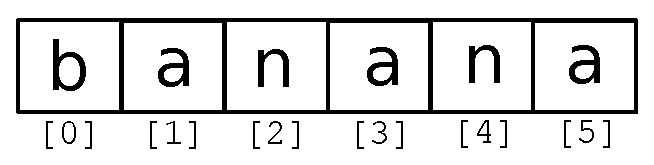
\includegraphics[height=0.50in]{figs2/string.eps}}
\afterfig

%\index{index!starting at zero}
\index{índice!iniciando no zero}
%\index{zero, index starting at}
\index{zero, índice do começo}

%You can use any expression, including variables and operators, as an
%index, but the value of the index has to be an integer.  Otherwise you
%get:

Você pode utilizar qualquer expressão, variável e operador, como um índice,
mas o valor do índice tem que ser um inteiro. Caso contrário você terá:

%\index{index}
\index{índice}
\index{exception!TypeError}
\index{TypeError}

\beforeverb
\begin{verbatim}
>>> letter = fruit[1.5]
TypeError: string indices must be integers
\end{verbatim}
\afterverb
%

%\section{Getting the length of a string using {\tt len}}
\section{Obtendo o tamanho de uma {\it string} usando {\tt len}}

%\index{len function}
%\index{function!len}
\index{função len}
\index{função!len}

{%\tt len} is a built-in function that returns the number of characters
%in a string:
A função {\tt len} nativa do Python, que retorna o número de caracteres de
uma {\it string}:

\beforeverb
\begin{verbatim}
>>> fruit = 'banana'
>>> len(fruit)
6
\end{verbatim}
\afterverb
%
%To get the last letter of a string, you might be tempted to try something
%like this:
%
Para obter a última letra da {\it string}, você pode tentar fazer algo como
isto:

%\index{exception!IndexError}
%\index{IndexError}
\index{excessão!IndexError}
\index{IndexError}

\beforeverb
\begin{verbatim}
>>> length = len(fruit)
>>> last = fruit[length]
IndexError: string index out of range
\end{verbatim}
\afterverb
%
%The reason for the {\tt IndexError} is that there is no letter in {\tt
%'banana'} with the index 6.  Since we started counting at zero, the
%six letters are numbered 0 to 5.  To get the last character, you have
%to subtract 1 from {\tt length}:
%
A razão para o {\tt IndexError} é que não existe letra em banana no índice 6.
Uma vez que começamos a contar a partir do zero, a seis letras são numeradas
de 0 até 5. Para mostrar o último caractere, você tem que subtrair 1 do 
tamanho ({\tt length}):

\beforeverb
\begin{verbatim}
>>> last = fruit[length-1]
>>> print last
a
\end{verbatim}
\afterverb
%
%Alternatively, you can use negative indices, which count backward from
%the end of the string.  The expression {\tt fruit[-1]} yields the last
%letter, {\tt fruit[-2]} yields the second to last, and so on.
%
Como alternativa, é possível utilizar índices negativos, que contam a string
de trás pra frente. A expressão {\tt fruit[-1]} mostra a última letra, 
{\tt fruit[-2]} mostra a segunda a partir do final, e assim por diante.

%\index{index!negative}
%\index{negative index}
\index{índice!negativo}
\index{índice negativo}

%\section{Traversal through a string with a loop}
\label{for}
\section{Percorrendo uma {\it string} com um {\it loop} }
%\index{traversal}
%\index{loop!traversal}
%\index{for loop}
%\index{loop!for}
%\index{statement!for}
\index{percorrer}
\index{laço!percorrer}
\index{laço for}
\index{laço!for}
\index{declaração!for}

%A lot of computations involve processing a string one character at a
%time.  Often they start at the beginning, select each character in
%turn, do something to it, and continue until the end.  This pattern of
%processing is called a {\bf traversal}.  One way to write a traversal
%is with a {\tt while} loop:

Processar uma string, um caractere por vez, envolve uma série de computação.
Normalmente, eles começam no começo da palavra, selecionam um caractere por
vez, fazem alguma coisa com ele, e continuam até o final. Este padrão de
processamento é chamado de {\bf percorrer}. Uma forma de percorrer uma 
{\it string}, por exemplo, é através de um loop com {\tt while}:

\beforeverb
\begin{verbatim}
index = 0
while index < len(fruit):
    letter = fruit[index]
    print letter
    index = index + 1
\end{verbatim}
\afterverb
%
%This loop traverses the string and displays each letter on a line by
%itself.  The loop condition is {\tt index < len(fruit)}, so
%when {\tt index} is equal to the length of the string, the
%condition is false, and the body of the loop is not executed.  The
%last character accessed is the one with the index {\tt len(fruit)-1},
%which is the last character in the string.
%
Este loop percorre a string e apresenta cada letra em uma linha própria. A
condição do loop é {\tt índice < len(fruit)}, assim quando o {\tt índice} for
igual ao tamanho da {\it string}, a condição se torna falsa, e o loop não é
executado. O último caractere acessado é o caractere com o índice
{\tt len(fruit)-1}, que é o último caractere na {\it string}.

\begin{ex}
%Write a {\tt while} loop that starts at the last character in the string
%and works its way backwards to the first character in the string, 
%printing each letter on a separate line, except backwards.

Escreva um loop {\tt while} que comece no último caractere da string e volte
de trás pra frente até o primeiro caractere da string, imprimindo cada letra
em uma linha separada.
\end{ex}

%Another way to write a traversal is with a {\tt for} loop:

Outra forma de percorrer uma string é com um loop {\tt for}:

\beforeverb
\begin{verbatim}
for char in fruit:
    print char
\end{verbatim}
\afterverb
%
%Each time through the loop, the next character in the string is assigned
%to the variable {\tt char}.  The loop continues until no characters are
%left.

Cada vez que percorrer o loop, o caractere na string é atribuido a variável
{\tt char}. O loop continua até que não haja mais caractere na string.


%\section{String slices}
\section{Fatiando {\it strings}}
%\label{slice}
\label{fatia}

%\index{slice operator}
%\index{operator!slice}
%\index{index!slice}
%\index{string!slice}
%\index{slice!string}
\index{operador fatiador}
\index{operador!fatia}
\index{índice!fatia}
\index{string!índice}
\index{fatia!string}

%A segment of a string is called a {\bf slice}.  Selecting a slice is
%similar to selecting a character:

Um segmento de uma string é chamado de {\bf fatia}. Selecionar uma fatia
é similar a selecionar um caractere:

\beforeverb
\begin{verbatim}
>>> s = 'Monty Python'
>>> print s[0:5]
Monty
>>> print s[6:12]
Python
\end{verbatim}
\afterverb
%
%The operator {\tt [n:m]} returns the part of the string from the 
%``n-eth'' character to the ``m-eth'' character, including the first but
%excluding the last.
%
O operador {\tt[n:m]} retorna a parte da string da posição ``n'' até a
posição ``m'', incluindo o primeiro, mas excluindo o último.

%If you omit the first index (before the colon), the slice starts at
%the beginning of the string.  If you omit the second index, the slice
%goes to the end of the string:

Se você omitir o primeiro índice (antes dos dois pontos), a fatia inicia no
começo da string. Se você omitir o segundo índice, a fatia irá até o fim da
string:

\beforeverb
\begin{verbatim}
>>> fruit = 'banana'
>>> fruit[:3]
'ban'
>>> fruit[3:]
'ana'
\end{verbatim}
\afterverb
%
%If the first index is greater than or equal to the second the result
%is an {\bf empty string}, represented by two quotation marks:

Se o primeiro índice for maior ou igual ao segundo, o resultado é uma
{\bf string vazia}, representado entre duas aspas.

%\index{quotation mark}
\index{aspa}

\beforeverb
\begin{verbatim}
>>> fruit = 'banana'
>>> fruit[3:3]
''
\end{verbatim}
\afterverb
%
%An empty string contains no characters and has length 0, but other
%than that, it is the same as any other string.
%
Uma string vazia não contém caracteres e tem tamanho 0 (zero), mas diferente
disto, isto é igual a qualquer outra string.

\begin{ex}
%Given that {\tt fruit} is a string, what does
%{\tt fruit[:]} mean?
Dada uma string, {\tt fruit}, o que significa a declaração {\tt fruit[:]}?
%\index{copy!slice}
%\index{slice!copy}
\index{cópia!fatia}
\index{fatia!copia}
\end{ex}

%\section{Strings are immutable}
\section{Strings são imutáveis}
%\index{mutability}
%\index{immutability}
%\index{string!immutable}
\index{mutabilidade}
\index{imutabilidade}
\index{string!imutabilidade}

%It is tempting to use the {\tt []} operator on the left side of an
%assignment, with the intention of changing a character in a string.
%For example:

É tentador utilizar o operador {\tt []} no lado esquerdo de uma atribuição,
com a intenção de mudar um caractere em uma string. Por exemplo:
\index{TypeError}
\index{exception!TypeError}

\beforeverb
\begin{verbatim}
>>> greeting = 'Hello, world!'
>>> greeting[0] = 'J'
TypeError: object does not support item assignment
\end{verbatim}
\afterverb
%
%The ``object'' in this case is the string and the ``item'' is
%the character you tried to assign.  For now, an {\bf object} is
%the same thing as a value, but we will refine that definition
%later.  An {\bf item} is one of the values in a sequence.
%
O ``objeto'' nesse caso é a string e o ``item'' é o caractere que você tentou
atribuir. Agora, um {\bf objeto} é a mesma coisa que um valor, mas vamos
refinar esta definição posteriormente. Um {\bf item} é um dos valores em uma
sequência.

%\index{object}
%\index{item assignment}
%\index{assignment!item}
%\index{immutability}
\index{objeto}
\index{ítem atribuido}
\index{atribuição!item}
\index{imutabilidade}

%The reason for the error is that
%strings are {\bf immutable}, which means you can't change an
%existing string.  The best you can do is create a new string
%that is a variation on the original:

A razão para o erro é que strings são {\bf imutáveis}, que significa que você
não pode mudar uma string já existente. O melhor que você pode fazer é criar
uma nova string que é uma variação da original:

\beforeverb
\begin{verbatim}
>>> greeting = 'Hello, world!'
>>> new_greeting = 'J' + greeting[1:]
>>> print new_greeting
Jello, world!
\end{verbatim}
\afterverb
%
%This example concatenates a new first letter onto
%a slice of {\tt greeting}.  It has no effect on
%the original string.
%
Neste exemplo, concatenamos uma nova letra em uma fatia de {\tt greeting}.
Isto não tem efeito na string original.

%\index{concatenation}
\index{concatenação}

%\section{Looping and counting}
\section{Looping e contabilização}
%\label{counter}
\label{contador}

%\index{counter}
\index{contador}

\index{counting and looping}
\index{looping and counting}
\index{looping!with strings}

\index{contando e rodando}
\index{rodando e contando}
\index{rodando!com string}

%The following program counts the number of times the letter {\tt a}
%appears in a string:

O programa a seguir conta o número de vezes que a letra {\tt a} aparece em
uma string:

\beforeverb
\begin{verbatim}
word = 'banana'
count = 0
for letter in word:
    if letter == 'a':
        count = count + 1
print count
\end{verbatim}
\afterverb
%
%This program demonstrates another pattern of computation called a {\bf
%counter}.  The variable {\tt count} is initialized to 0 and then
%incremented each time an {\tt a} is found.
%When the loop exits, {\tt count}
%contains the result---the total number of {\tt a}'s.
%
Este programa demonstra outro padrão de computação chamado {\bf contador}. A
variável {\tt count} é iniciada em 0 e depois incrementada cada vez que uma
letra {\tt a} é encontrada. Quando o laço existe, {\tt count} contém o
resultado---o número total de {\tt a}'s.

\begin{ex}
%\index{encapsulation}
\index{encapsulamento}

%Encapsulate this code in a function named {\tt
%count}, and generalize it so that it accepts the string and the
%letter as arguments.

Encapsule este código em uma função chamada {\tt count}, e generalize para
que aceite a string e a letra como argumento.
\end{ex}

%\section{The {\tt in} operator}
%\label{inboth}
\section{O operador {\tt in}}
\label{inboth}

%\index{in operator}
%\index{operator!in}
%\index{boolean operator}
%\index{operator!boolean}
\index{operador in}
\index{operador!in}
\index{operador booleano}
\index{operador!booleano}

%The word {\tt in} is a boolean operator that takes two strings and
%returns {\tt True} if the first appears as a substring in the second:

A palavra {\tt in} é um operador booleano que pega duas strings e retorna
{\tt True} se a primeira aparecer como substring na segunda:

\beforeverb
\begin{verbatim}
>>> 'a' in 'banana'
True
>>> 'seed' in 'banana'
False
\end{verbatim}
\afterverb
%

%\section{String comparison}
\section{Comparação de string}

%\index{string!comparison}
%\index{comparison!string}
\index{string!comparação}
\index{comparação!index}

%The comparison operators work on strings.  To see if two strings are equal:

O operador de comparação funciona com strings. Para verificar se duas strings
são iguais:

\beforeverb
\begin{verbatim}
if word == 'banana':
    print  'All right, bananas.'
\end{verbatim}
\afterverb
%
%Other comparison operations are useful for putting words in alphabetical
%order:
%
Outras operações de comparações são úteis para colocar as palavras em ordem
alfabética:

\beforeverb
\begin{verbatim}
if word < 'banana':
    print 'Your word,' + word + ', comes before banana.'
elif word > 'banana':
    print 'Your word,' + word + ', comes after banana.'
else:
    print 'All right, bananas.'
\end{verbatim}
\afterverb
%
%Python does not handle uppercase and lowercase letters the same way
%that people do.  All the uppercase letters come before all the
%lowercase letters, so:
%
Python não manipula letras em maiúscula ou minúscula da mesma forma que as
pessoas fazem. Todas as palavras em maiúsculas vem antes das minúsculas, então:

\beforeverb
\begin{verbatim}
%Your word, Pineapple, comes before banana.
Sua palavra, Abacaxi, vem antes de banana.
\end{verbatim}
\afterverb
%
%A common way to address this problem is to convert strings to a
%standard format, such as all lowercase, before performing the
%comparison.  Keep that in mind in case you have to defend yourself
%against a man armed with a Pineapple.
%
Uma maneira de tratar este problema é converter strings para um formato
padrão, todas como minúsculas, antes de realizar a comparação. Mantenha isto
em mente em caso de ter que se defender contra alguém armado com um abacaxi.

%\section{{\tt string} methods}
\section{Método {\tt string}}
%Strings are an example of Python {\bf objects}.  An object contains
%both data (the actual string itself) and {\bf methods}, which
%are effectively functions that are built into the object and 
%are available to any {\bf instance} of the object.

Strings são um exemplo de um {\bf objeto} em Python. Um objeto contém ambos
dado (a string atual) e os {\bf métodos}, que são efetivamente funções
construídas dentro do objeto e disponível para quaisquer instâncias do objeto.

%Python has a function called {\tt dir} which lists the methods available
%for an object.  The {\tt type} function shows the type of an object 
%and the {\tt dir} function shows the available methods.

Python tem uma função chamada {\tt dir} que lista os métodos disponíveis de
um objeto. A função {\tt type} mostra o tipo de um objeto e a função {\tt dir}
os métodos disponíveis.

\beforeverb
\begin{verbatim}
>>> stuff = 'Hello world'
>>> type(stuff)
<type 'str'>
>>> dir(stuff)
['capitalize', 'center', 'count', 'decode', 'encode',
'endswith', 'expandtabs', 'find', 'format', 'index',
'isalnum', 'isalpha', 'isdigit', 'islower', 'isspace',
'istitle', 'isupper', 'join', 'ljust', 'lower', 'lstrip',
'partition', 'replace', 'rfind', 'rindex', 'rjust',
'rpartition', 'rsplit', 'rstrip', 'split', 'splitlines',
'startswith', 'strip', 'swapcase', 'title', 'translate',
'upper', 'zfill']
>>> help(str.capitalize)
Help on method_descriptor:

capitalize(...)
    S.capitalize() -> string

    Return a copy of the string S with only its first character
    capitalized.
>>>
\end{verbatim}
\afterverb
%

%While the {\tt dir} function lists the methods, and you 
%can use {\tt help} to get some simple documentation on a method, 
%a better source of documentation for string methods would be
%\url{https://docs.python.org/2/library/stdtypes.html#string-methods}.

A função {\tt dir} lista os métodos, e você pode utilizar {\tt help}
para obter ajuda na documentação de um método, uma melhor fonte de
documentação para métodos de string pode ser vista através do endereço
\url{https://docs.python.org/2/library/stdtypes.html#string-methods}.

%Calling a {\bf method} is similar to calling a function---it 
%takes arguments and returns a value---but the syntax is different.
%We call a method by appending the method name to the variable name
%using the period as a delimiter.

Chamar um {\bf método} é similar a chamar uma função---recebe argumentos e
retorna um valor---mas a sintaxe é diferente. Nós chamamos um método anexando
o nome do método a variável utilizando um ponto como delimitador.

%For example, the
%method {\tt upper} takes a string and returns a new string with
%all uppercase letters:

Por exemplo, o método {\tt upper} transforma uma string, retornando uma nova
string com todas as letras em maiúsculo:

%\index{method}
%\index{string!method}
\index{método}
\index{string!método}

%Instead of the function syntax {\tt upper(word)}, it uses
%the method syntax {\tt word.upper()}.
Ao invés de usar a sintaxe de uma função {\tt upper(word)}, usa-se a sintaxe
de método {\tt word.upper()}.

%\index{dot notation}
\index{notação de ponto}

\beforeverb
\begin{verbatim}
>>> word = 'banana'
>>> new_word = word.upper()
>>> print new_word
BANANA
\end{verbatim}
\afterverb
%
%This form of dot notation specifies the name of the method, {\tt
%upper}, and the name of the string to apply the method to, {\tt
%word}.  The empty parentheses indicate that this method takes no
%argument.
%
Esta forma de notação de ponto especifica o nome do método, {\tt upper}, e
o nome da string para aplicar o método, {\tt word}. O parêntese vazio indica
que este método não recebe argumento.

%\index{parentheses!empty}
\index{parênteses!vazio}

%A method call is called an {\bf invocation}; in this case, we would
%say that we are invoking {\tt upper} on the {\tt word}.

Uma chamado de método é dito como uma {\bf invocação}; neste caso, podemos
dizer que estamos invocando {\tt upper} na palavra {\tt word}.

%\index{invocation}
\index{invocação}

%For example, there is a string method named {\tt find} that
%searches for the position of one string within another:

Por exemplo, existe um método de string chamado {\tt find} que procura pela
posição de uma string em outra:

\beforeverb
\begin{verbatim}
>>> word = 'banana'
>>> index = word.find('a')
>>> print index
1
\end{verbatim}
\afterverb
%
%In this example, we invoke {\tt find} on {\tt word} and pass
%the letter we are looking for as a parameter.
%
Neste exemplo, nós invocamos {\tt find} na palavra {\tt word} e passamos a
letra que estamos procurando como um parâmetro.

%The {\tt find} method can find substrings as well as characters:

O método {\tt find} consegue encontrar substrings, assim como caracteres:

\beforeverb
\begin{verbatim}
>>> word.find('na')
2
\end{verbatim}
\afterverb
%
%It can take as a second argument the index where it should start:
%
Pode receber como segundo argumento, o índice que indica onde deve começar:

%\index{optional argument}
%\index{argument!optional}
\index{argumento opcional}
\index{argumento!opcional}

\beforeverb
\begin{verbatim}
>>> word.find('na', 3)
4
\end{verbatim}
\afterverb
%
%One common task is to remove white space (spaces, tabs, or newlines) from
%the beginning and end of a string using the {\tt strip} method:
%
Uma tarefa comum é remover espaços em branco (espaços, tabs ou novas
linhas) do início e final de uma string é usado o método {\tt strip}:

\beforeverb
\begin{verbatim}
>>> line = '  Here we go  '
>>> line.strip()
'Here we go'
\end{verbatim}
\afterverb
%
%Some methods such as {\bf startswith} return boolean values.
%
Alguns métodos como o {\bf startswith} retorna valores booleanos.

\beforeverb
\begin{verbatim}
>>> line = 'Please have a nice day'
>>> line.startswith('Please')
True
>>> line.startswith('p')
False
\end{verbatim}
\afterverb
%
%You will note that {\tt startswith} requires case to match, so sometimes
%we take a line and map it all to lowercase before we do any checking
%using the {\tt lower} method.
%
Você perceberá que {\tt startswith} precisa ser case sensitive para funcionar, 
então algumas vezes nós pegamos uma linha e convertemos para minúscula antes 
de fazer qualquer verificação, utilizando o método {\tt lower}.

\beforeverb
\begin{verbatim}
>>> line = 'Please have a nice day'
>>> line.startswith('p')
False
>>> line.lower()
'please have a nice day'
>>> line.lower().startswith('p')
True
\end{verbatim}
\afterverb
%
%In the last example, the method {\tt lower} is called
%and then we use {\tt startswith}
%to see if the resulting lowercase string
%starts with the letter ``p''.  As long as we are careful
%with the order, we can make multiple method calls in a
%single expression.
%
No último exemplo, o método {\tt lower} é chamado e depois utilizamos
{\tt startswith} para verificar se a string resultante em minúsculo começa
com a letra ``p''. Contanto que nos preocupemos com a ordem, podemos realizar
múltiplas chamadas de métodos em uma única expressão.

\begin{ex}
%\index{count method}
%\index{method!count}
\index{método contador}
\index{método!contador}

%There is a string method called {\tt count} that is similar
%to the function in the previous exercise.  Read the documentation
%of this method at
%\url{https://docs.python.org/2/library/stdtypes.html#string-methods}
%and write an invocation that counts the number of times the 
%letter a  occurs
%in \verb"'banana'".

Existe um método de strings chamado {\tt count} que é similar a função do
exercício anterior. Leia a documentação deste método no endereço:
\url{https://docs.python.org/2/library/stdtypes.html#string-methods}
e escreva uma invocação que conte o número de vezes que a letra ``a'' ocorre
em \verb"'banana'".
\end{ex}

%\section{Parsing strings}
\section{Analisando strings}

%Often, we want to look into a string and find a substring.  For example
%if we were presented a series of lines formatted as follows:

Normalmente queremos olhar uma string e procurar uma substring. Por exemplo
se forem apresentadas uma série de linhas formatadas como a seguir:

\beforeverb
\begin{alltt}
From stephen.marquard@{\bf uct.ac.za} Sat Jan  5 09:14:16 2008
\end{alltt}
\afterverb

%and we wanted to pull out only the second half of the address (i.e.,
%{\tt uct.ac.za}) from each line, we can do this by using the {\tt find}
%method and string slicing.

e quisermos tirar somente a segunda metade do endereço (i.e., {\tt uct.ac.za})
de cada linha, nós podemos fazer isto utilizando o método {\tt find}, fatiando
a string.

%First, we will find the position of the at-sign in the string.  Then we will
%find the position of the first space \emph{after} the at-sign.  And then we
%will use string slicing to extract the portion of the string which we 
%are looking for.

Primeiro, nós encontraremos a posição do arroba (``@'') na string. Depois
acharemos a posição do primeiro espaço, \emph{depois} do arroba. E então usaremos
o fatiamento da string para extrair a porção da string que estamos procurando.

\beforeverb
\begin{verbatim}
>>> data = 'From stephen.marquard@uct.ac.za Sat Jan  5 09:14:16 2008'
>>> atpos = data.find('@')
>>> print atpos
21
>>> sppos = data.find(' ',atpos)
>>> print sppos
31
>>> host = data[atpos+1:sppos]
>>> print host
uct.ac.za
>>> 
\end{verbatim}
\afterverb
%
%We use a version of the {\tt find} method which allows us to specify
%a position in the string where we want {\tt find} to start looking.
%When we slice, we extract the characters 
%from ``one beyond the at-sign through up to \emph{but not including} the 
%space character''.  
%
Utilizamos uma versão do método {\tt find}, que nos permite especificar uma
posição na string, onde queremos começar a procura. Quando fatiamos, extraímos
os caracteres de ``um além do arroba até \emph{mas não incluindo} o caractere
espaço''.

%The documentation for the {\tt find} method is available at
%\url{https://docs.python.org/2/library/stdtypes.html#string-methods}.

A documentação para o método {\tt find} está disponível no endereço
\url{https://docs.python.org/2/library/stdtypes.html#string-methods}.

%\section{Format operator}
\section{Operador format}

%\index{format operator}
\index{operator!format}

%The {\bf format operator}, {\tt \%}
%allows us to construct strings, replacing parts of the strings
%with the data stored in variables.
%When applied to integers, {\tt \%} is the modulus operator.  But
%when the first operand is a string, {\tt \%} is the format operator.

O operador {\bf format}, {\tt \%} nos permite construir strings, substituindo
parte da string com dados armazenados em variáveis. Quando aplicados a
inteiros, o {\tt \%} é o operador módulo. Mas quando o primeiro operando é
uma string, o {\tt \%} é o operador {\tt format}.

%\index{format string}
\index{formatar string}

%The first operand is the {\bf format string}, which contains
%one or more {\bf format sequences} that specify how
%the second operand is formatted.  The result is a string.

O primeiro operando é o {\bf format} de string, que contém uma ou mais
{\bf sequências} que especifica como o segundo operador é formatado. O
resultado é uma string.

%\index{format sequence}
\index{sequência format}

%For example, the format sequence \verb"'%d'" means that
%the second operand should be formatted as an
%integer ({\tt d} stands for ``decimal''):

Por exemplo, a sequência de formatação \verb"'%d'" significa que o segundo
operando deve ser formatado como um inteiro ({\tt d} significa ``decimal''):

\beforeverb
\begin{verbatim}
>>> camels = 42
>>> '%d' % camels
'42'
\end{verbatim}
\afterverb
%
%The result is the string \verb"'42'", which is not to be confused
%with the integer value {\tt 42}.
%
O resultado é a string \verb"'42'", que não pode ser confundido com o valor
inteiro {\tt 42}.

%A format sequence can appear anywhere in the string,
%so you can embed a value in a sentence:

Um sequência de {\tt format} pode aparecer em qualquer lugar em uma string,
então você pode embutir um valor em uma sequência:

\beforeverb
\begin{verbatim}
>>> camels = 42
>>> 'I have spotted %d camels.' % camels
'I have spotted 42 camels.'
\end{verbatim}
\afterverb
%
%If there is more than one format sequence in the string,
%the second argument has to be a tuple\footnote{A tuple is a
%sequence of comma-separated values inside a pair of brackets.
%We will cover tuples in Chapter 10}.  Each format sequence is
%matched with an element of the tuple, in order.
%
Se houver mais de uma sequência de {\tt format} na string, o segundo argumento
tem que ser uma tupla\footnote{Um tupla é uma sequência de valores, separados
	por vírgula dentro de um par de colchetes. Vamos abordar tuplas no
	Capítulo 10}. Cada sequência de {\tt format} é combinada com um elemento
da tupla, em ordem.

%The following example uses \verb"'%d'" to format an integer,
%\verb"'%g'" to format
%a floating-point number (don't ask why), and \verb"'%s'" to format
%a string:

O seguinte exemplo utiliza \verb"'%d'" para formatar um inteiro, o
\verb"'%g'" para formatar um ponto-flutuante (não pergunte o por quê), e
\verb"'%s'" para formatar string:

\beforeverb
\begin{verbatim}
>>> 'In %d years I have spotted %g %s.' % (3, 0.1, 'camels')
'In 3 years I have spotted 0.1 camels.'
\end{verbatim}
\afterverb
%
%The number of elements in the tuple must match the number
%of format sequences in the string.  The types of the
%elements also must match the format sequences:
%
O número de elementos na tupla deve combinar com o número de sequência
para formatar em uma string. Os tipos de elementos também devem combinar
com a sequência a ser formatada:

\index{exception!TypeError}
\index{TypeError}

\beforeverb
\begin{verbatim}
>>> '%d %d %d' % (1, 2)
TypeError: not enough arguments for format string
>>> '%d' % 'dollars'
TypeError: illegal argument type for built-in operation
\end{verbatim}
\afterverb
%
%In the first example, there aren't enough elements; in the
%second, the element is the wrong type.
%
No primeiro exemplo, não existem elementos suficientes; no segundo o elemento
possui o tipo errado.

%The format operator is powerful, but it can be difficult to use.  You
%can read more about it at
%\url{https://docs.python.org/2/library/stdtypes.html#string-formatting}.

O operador {\tt format} é muito poderoso, mas pode ser difícil de ser
utilizado. Você pode ler mais sobre ele no endereço
\url{https://docs.python.org/2/library/stdtypes.html#string-formatting}.

% You can specify the number of digits as part of the format sequence.
% For example, the sequence \verb"'%8.2f'"
% formats a floating-point number to be 8 characters long, with
% 2 digits after the decimal point:

Você pode especificar o número de dígitos como parte do formato de uma sequência.
Por exemplo, a sequência \verb"'%8.2f'"
formata um número em ponto flutuante para ter 8 caracteres de comprimento, com
2 dígitos depois do ponto decimal:

\beforeverb
\begin{verbatim}
>>> '%8.2f' % 3.14159
'    3.14'
\end{verbatim}
\afterverb
%
%The result takes up eight spaces with two
%digits after the decimal point.  

O resultado ocupa oito casas com dois dígitos
depois do ponto decimal;

%\section{Debugging}
\section{Depurando}
%\index{debugging}
\index{depuração}

%A skill that you should cultivate as you program is always
%asking yourself, ``What could go wrong here?'' or alternatively,
%``What crazy thing might our user do to crash our (seemingly) 
%perfect program?''

Uma habilidade que você deve cultivar como programador é se perguntar sempre
``O que poderia dar errado?'' ou alternativamente, ``Que coisa louca nosso
usuário pode fazer para quebrar nosso programa (aparentemente) perfeito?''.

%For example, look at the program which we used to demonstrate
%the {\tt while} loop in the chapter on iteration:

Por exemplo, olhe para o programa que utilizamos para demonstrar o laço
{\tt while} no capítulo de iterações:

\beforeverb
\begin{verbatim}
while True:
    line = raw_input('> ')
    if line[0] == '#' :
        continue
    if line == 'done':
        break
    print line

print 'Done!'
\end{verbatim}
\afterverb
%
%Look what happens when the user enters an empty line of input:
%
Olhe o que acontece quando o usuário entrar com uma linha em branco no
{\tt input}:

\beforeverb
\begin{verbatim}
> hello there
hello there
> # don't print this
> print this!
print this!
>
Traceback (most recent call last):
  File "copytildone.py", line 3, in <module>
    if line[0] == '#' :
\end{verbatim}
\afterverb
%
%The code works fine until it is presented an empty line.  Then
%there is no zero-th character, so we get a traceback.  There are two
%solutions to this to make line three ``safe'' even if the line is 
%empty.
%

O código funciona, até que se use uma linha vazia. Então existe um caractere
não zero, e assim recebemos um {\tt traceback}. Existem duas soluções para isto
para tornar a linha três ``segura'' mesmo se a linha estiver vazia.

%One possibility is to simply use the {\tt startswith} method
%which returns {\tt False} if the string is empty.

Uma possibilidade é utilizando o método {\tt startswith} que retorna
{\tt False} se a string estiver vazia.

\beforeverb
\begin{verbatim}
    if line.startswith('#') :
\end{verbatim}
\afterverb
%
%\index{guardian pattern}
%\index{pattern!guardian}
\index{padrão de guarda}
\index{padrão!guarda}

%Another way is to safely write the {\tt if} statement using the {\bf guardian}
%pattern and make sure the second logical expression is evaluated 
%only where there is at least one character in the string.:

Outra forma é escrever de forma segura uma condição de {\tt if} utilizando o
padrão de {\bf guarda} e garantir que a segunda expressão lógica seja avaliada
somente onde existe pelo menos um caractere na string:

\beforeverb
\begin{verbatim}
    if len(line) > 0 and line[0] == '#' :
\end{verbatim}
\afterverb
%

%\section{Glossary}
\section{Glossário}

\begin{description}

%\item[counter:] A variable used to count something, usually initialized
%to zero and then incremented.
\item[contador:] Uma variável utilizada para contar alguma coisa, normalmente
	inicializada em zero e depois incrementada.
%\index{counter}
\index{contador}

%\item[empty string:] A string with no characters and length 0, represented
%by two quotation marks.
%\index{empty string}
\item[string vazia:] Uma string sem caracteres e tamanho 0, representado por
	duas aspas.
\index{string vazia}

%\item[format operator:] An operator, {\tt \%}, that takes a format
%string and a tuple and generates a string that includes
%the elements of the tuple formatted as specified by the format string.
\item[operador format:] Um operador, {\tt \%}, que pega uma string formatada
	e uma tupla gerando um string que inclui elementos da tupla formatada
	especificada pela string formatada.
%\index{format operator}
%\index{operator!format}
\index{operador format}
\index{operador!format}

%\item[format sequence:] A sequence of characters in a format string,
%like {\tt \%d}, that specifies how a value should be formatted.
\item[sequência formatada:] Uma sequência de caracteres em uma string formatada,
	como {\tt \%d}. que especifica como um valor deve ser formatado.
%\index{format sequence}
\index{sequência formatadas}

%\item[format string:] A string, used with the format operator, that
%contains format sequences.
%\index{format string}

\item[string formatada:] Uma string, utilizada com o operador {\tt format},
	que contém uma sequência formatada.

\index{string formatada}

%\item[flag:] A boolean variable used to indicate whether a condition
%is true.
\item[flag:] Uma variável booleana utilizada para indicar se uma condição é
	verdadeira.
\index{flag}

%\item[invocation:] A statement that calls a method.
%\index{invocation}
\item[invocação:] Uma condição que chama um método.
\index{invocação}

%\item[immutable:] The property of a sequence whose items cannot
%be assigned.
%\index{immutability}
\item[imutável:] Propriedades de uma sequência dos itens que não podem ser
	atribuídos.
\index{imutabilidade}

%\item[index:] An integer value used to select an item in
%a sequence, such as a character in a string.
%\index{index}
\item[índice:] Um valor inteiro usado para selecionar um item em uma sequência,
	como um caractere em uma string.
\index{índice}

%\item[item:] One of the values in a sequence.
%\index{item}

\item[item:] Um dos valores em uma sequência.
\index{item}

%\item[method:] A function that is associated with an object and called
%using dot notation.
%\index{method}
\item[método:] Uma função que é associada com um objeto e acessado utilizando
	a notação de ponto.
\index{método}

%\item[object:] Something a variable can refer to.  For now,
%you can use ``object'' and ``value'' interchangeably.
%\index{object}

\item[objeto:] Algum valor ao qual uma variável se refere. Desta forma você pode
	utilizar ``objeto'' e ``valor'' de forma intercambiável.
\index{objeto}

%\item[search:] A pattern of traversal that stops
%when it finds what it is looking for.
\item[procura:] Um padrão que percorre transversalmente e para quando 
  encontra o que está procurando.
%\index{search pattern}
%\index{pattern!search}
\index{padrão pesquisa}
\index{padrão!pesquisa}

%\item[sequence:] An ordered set; that is, a set of
%values where each value is identified by an integer index.
%\index{sequence}
\item[sequência:] Um conjunto ordenado; que é, um conjunto de valores onde
	cada valor é identificado por um índice inteiro.
\index{sequência}

%\item[slice:] A part of a string specified by a range of indices.

%\index{slice}
\item[fatia:] Uma parte da string especificada por uma
\index{fatia}

%\item[traverse:] To iterate through the items in a sequence,
%performing a similar operation on each.
\item[percorrer:] Percorrer através de itens em uma sequência, executando uma
	operação similar em cada um dos itens.

%\index{traversal}
\index{percorrer}

\end{description}


%\section{Exercises}
\section{Exercícios}
\begin{ex}
%Take the following Python code that stores a string:`

Use o código Python a seguir para armazenar a string:`

\beforeverb
\begin{alltt}
str = 'X-DSPAM-Confidence: {\bf 0.8475}'
\end{alltt}
\afterverb

%Use {\tt find} and string slicing to extract the portion
%of the string after the colon character and then use the 
%{\tt float} function to convert the extracted string 
%into a floating point number.

Use o {\tt find} e o fatiamento de strings para extrair a parte da string
depois da vírgula e então use a função {\tt float} para converter a string
extraída em um número de ponto flutuante.
\end{ex}


\begin{ex}
%\index{string method}
%\index{method!string}
\index{métodos string}
\index{método!string}

%Read the documentation of the string methods at
%\url{https://docs.python.org/2/library/stdtypes.html#string-methods}.
%You might want to experiment with some of them to make sure
%you understand how they work.  {\tt strip} and
%{\tt replace} are particularly useful.

Leia a documentação dos métodos de {\tt string} no endereço 
\url{https://docs.python.org/2/library/stdtypes.html#string-methods}.
Você pode querer experimentar alguns destes métodos para ter certeza que
entendeu como funcionam. Por exemplo, {\tt strip} e {\tt replace} são
particularmente úteis.

%The documentation uses a syntax that might be confusing.
%For example, in \verb"find(sub[, start[, end]])", the brackets
%indicate optional arguments.  So {\tt sub} is required, but
%{\tt start} is optional, and if you include {\tt start},
%then {\tt end} is optional.

A documentação utiliza uma sintaxe que pode parecer confusa. Por exemplo, no
\verb"find(sub[, start[, end]])", os colchetes indicam que o argumento é
opcional. Desta forma, {\tt sub} é obrigatório, mas {\tt start} é opcional, e
se você incluir o {\tt start}, então o {\tt end} é opcional.

\end{ex}
% TODO % LaTeX source for ``Python for Informatics: Exploring Information''
% Copyright (c)  2010-  Charles R. Severance, All Rights Reserved

\chapter{Arquivos}
%\chapter{Files}

\index{arquivo}
\index{tipo!arquivo}
%\index{file}
%\index{type!file}

\section{Persistência}
%\section{Persistence}

\index{persistência}
\index{memória secundária}
%\index{persistence}
%\index{secondary memory}

Até agora, aprendemos como escrever programas e comunicar nossas
intenções para a {\bf Unidade de Processamento Central} usando execução
condicional, funções e iterações. Aprendemos também como criar e usar 
estruturas de dados na {\bf Memória Principal}. A CPU e a memória é onde
nosso software executa. É o lugar onde todo ``o pensamento'' acontece.
%So far, we have learned how to write programs and communicate 
%our intentions to the {\bf Central Processing Unit} using conditional
%execution, functions, and iterations.  We have learned how to 
%create and use data structures in the {\bf Main Memory}.  The CPU 
%and memory are where our software works and runs.  It is where 
%all of the ``thinking'' happens.  

Mas se você se recordar das nossas discussões sobre arquitetura de hardware,
uma vez que a energia for desligada, tudo que estiver armazenado na CPU
ou na memória principal será apagado. Até agora, nossos
programas tem sido breves exercícios para aprender Python.
%But if you recall from our hardware architecture discussions,
%once the power is turned off, anything stored in either
%the CPU or main memory is erased.  So up to now, our
%programs have just been transient fun exercises to learn Python.

\beforefig
\centerline{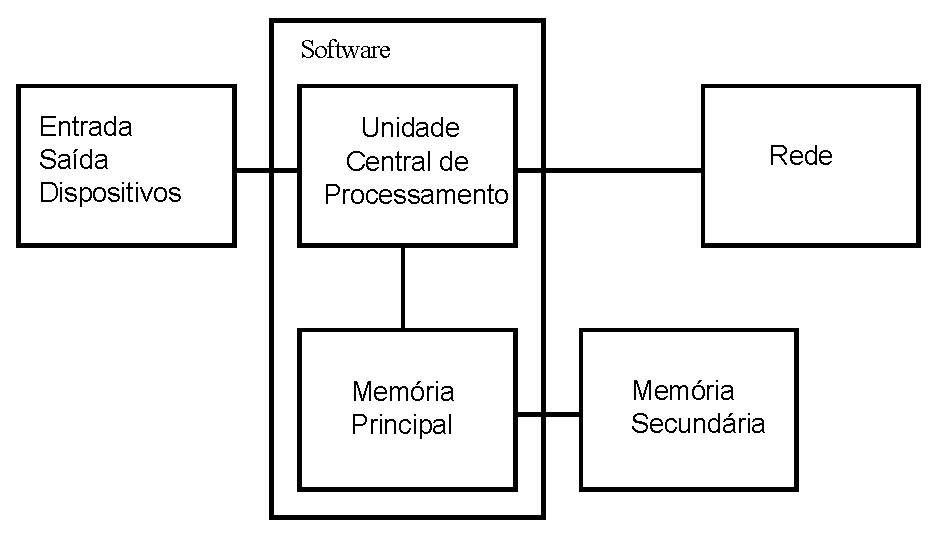
\includegraphics[height=2.50in]{figs2/arch3.eps}}
\afterfig
%\beforefig
%\centerline{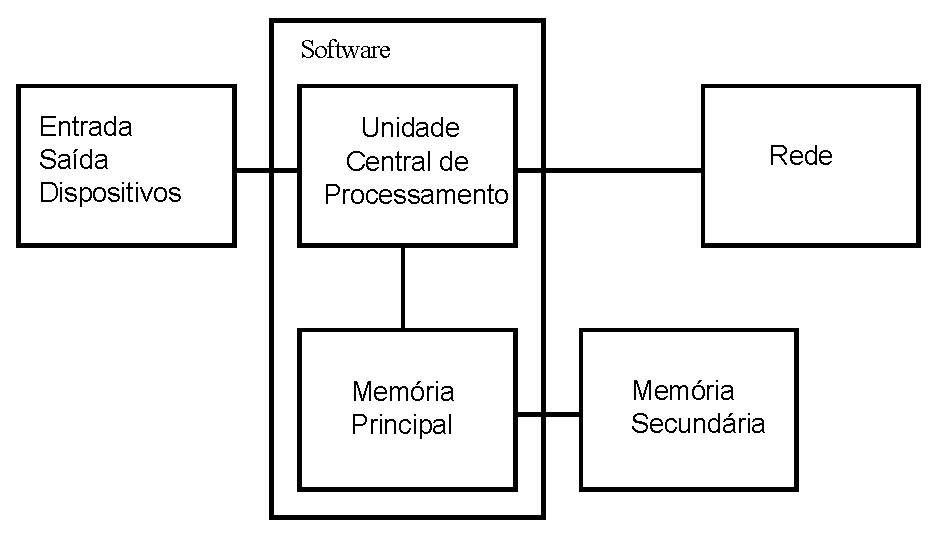
\includegraphics[height=2.50in]{figs2/arch3.eps}}
%\afterfig

Neste capítulo, começaremos a trabalhar com {\bf Memória Secundária}
(ou arquivos).
A memória secundária não é apagada quando a energia é desligada.
Ou no caso de um pen drive USB, o
dado que nós escrevemos a partir de nossos programas, pode ser
removido e transportado para outro sistema.
%In this chapter, we start to work with {\bf Secondary Memory} 
%(or files).
%Secondary memory is not erased even when the power is turned off.  
%Or in the case of a USB flash drive, the
%data we write from our programs can be removed from the 
%system and transported to another system.

Nós focaremos primeiramente na leitura e escrita de arquivos texto
tais como aqueles que criamos em um editor de texto. Depois iremos
trabalhar com arquivos de banco de dados que são arquivos binários,
especificamente desenhados para serem lidos e escritos através do nosso
software de banco de dados.
%We will primarily focus on reading and writing text files such as 
%those we create in a text editor.  Later we will see how to work
%with database files which are binary files, specifically designed to be read
%and written through database software.

\section{Lendo arquivos}
\index{arquivo!leitura}
\index{função open}
\index{função!open}
%\section{Opening files}
%\index{file!open}
%\index{open function}
%\index{function!open}

Quando queremos ler ou gravar um arquivo (nosso disco rígido, por exemplo),
devemos sempre abrir o arquivo primeiro através do comando {\bf open}. Abrir um
arquivo é uma comunicação com o seu sistema operacional, que sabe onde o dado
para cada arquivo é armazenado. Quando você abre um arquivo, você está pedindo
ao sistema operacional para encontrar o arquivo pelo nome e certificar-se de que
ele existe. Neste exemplo, abrimos o arquivo {\tt mbox.txt}, o qual deve ser armazenado
no mesmo diretório onde o seu programa Python está executando.
Você pode fazer o download deste arquivo a partir de:
\url{www.py4inf.com/code/mbox.txt}
%When we want to read or write a file (say on your hard drive), we first
%must {\bf open} the file.  Opening the file communicates with your operating
%system, which knows where the data for each file is stored.  When you open
%a file, you are asking the operating system to find the file by name
%and make sure the file exists.  In this example, we open the file 
%{\tt mbox.txt}, which should be stored in the same folder that you
%are in when you start Python.
%You can download this file from 
%\url{www.py4inf.com/code/mbox.txt}

\beforeverb
\begin{verbatim}
>>> fhand = open('mbox.txt')
>>> print fhand
<open file 'mbox.txt', mode 'r' at 0x1005088b0>
\end{verbatim}
\afterverb
%\beforeverb
%\begin{verbatim}
%>>> fhand = open('mbox.txt')
%>>> print fhand
%<open file 'mbox.txt', mode 'r' at 0x1005088b0>
%\end{verbatim}
%\afterverb
%

\index{manipulação de arquivo}
%\index{file handle}

Se o comando {\tt open} rodar com sucesso, o sistema operacional nos
retorna um {\bf manipulador de arquivo}. Este manipulador não contém
os dados do arquivo, mas apenas o ``ponteiro'' que nós podemos usar
para ler um dado. Você recebe um ponteiro se o arquivo requisitado
existir e se você tiver permissão para lê-lo.
%If the {\tt open} is successful, the operating system returns us a 
%{\bf file handle}.  The file handle is not the actual data contained
%in the file, but instead it is a ``handle'' that we can use to 
%read the data.   You are given a handle if the requested file
%exists and you have the proper permissions to read the file.

\beforefig
\centerline{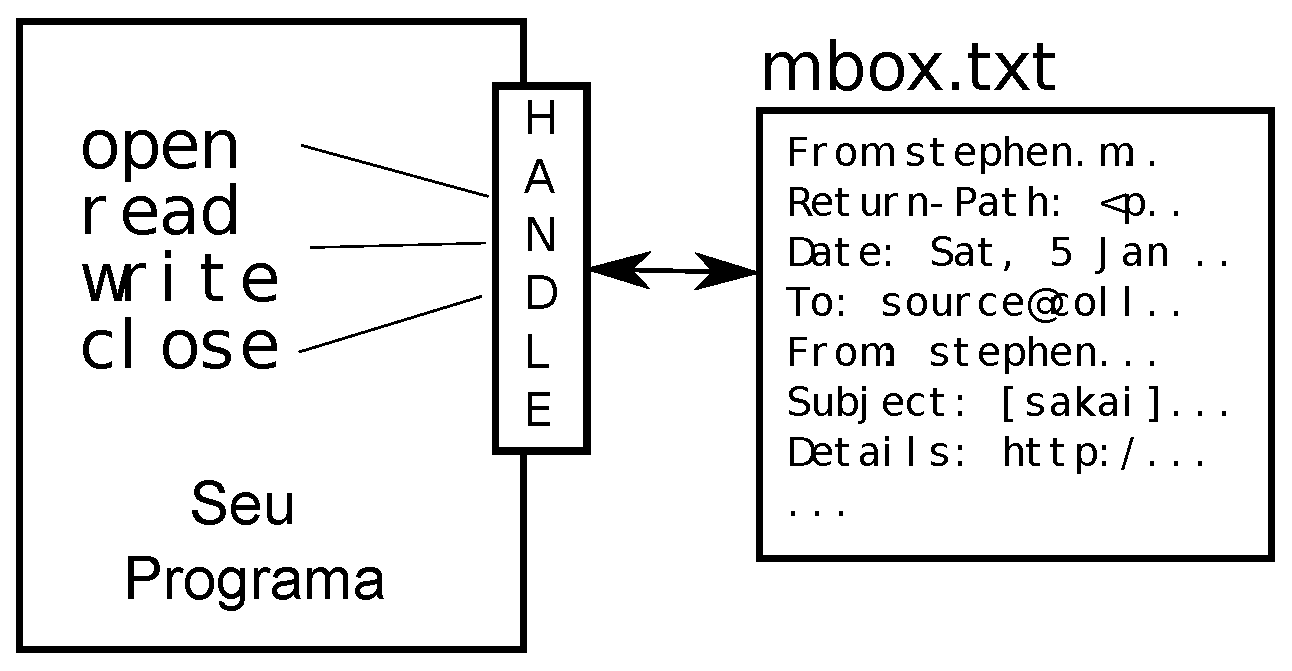
\includegraphics[height=1.75in]{figs2/handle.eps}}
\afterfig
%\beforefig
%\centerline{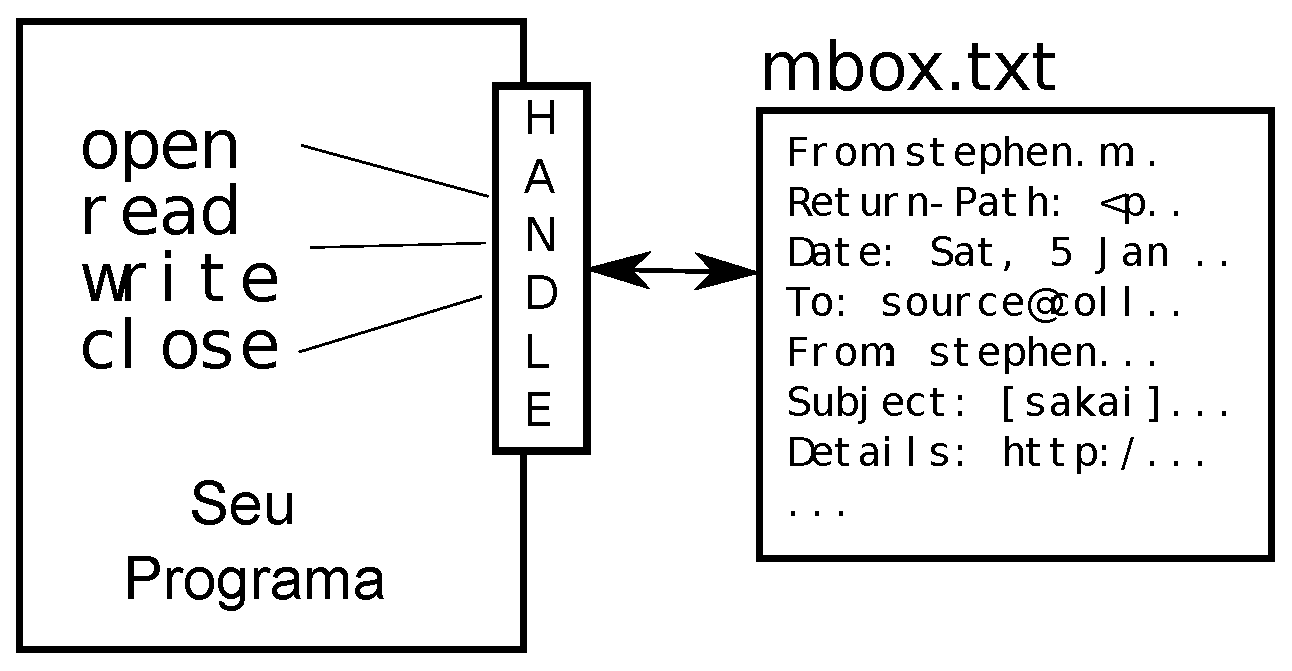
\includegraphics[height=1.75in]{figs2/handle.eps}}
%\afterfig

Se o arquivo não existir, {\tt open} ocorrerá um erro com a pilha de execução (traceback)
e você não conseguirá obter um ponteiro (handle) para acessar o conteúdo do arquivo: 
%If the file does not exist, {\tt open} will fail with a traceback and you 
%will not get a handle to access the contents of the file:

\beforeverb
\begin{verbatim}
>>> fhand = open('stuff.txt')
Traceback (most recent call last):
  File "<stdin>", line 1, in <module>
IOError: [Errno 2] No such file or directory: 'stuff.txt'
\end{verbatim}
\afterverb
%\beforeverb
%\begin{verbatim}
%>>> fhand = open('stuff.txt')
%Traceback (most recent call last):
%  File "<stdin>", line 1, in <module>
%IOError: [Errno 2] No such file or directory: 'stuff.txt'
%\end{verbatim}
%\afterverb

Mais tarde, vamos aprender a utilizar {\tt try} e {\tt except} para lidar 
com a situação onde tentamos abrir um arquivo que não existe.
%Later we will use {\tt try} and {\tt except} to deal more gracefully
%with the situation where we attempt to open a file that does 
%not exist.

\section{Arquivos texto e linhas}
%\section{Text files and lines}

Podemos imaginar um arquivo texto como um sequência de linhas, assim
como uma string em Python é uma sequência de caracteres. Por exemplo, esta
é um exemplo de um arquivo texto com registros de atividade de e-mail de várias
pessoas em um time de desenvolvimento em um projeto open source:
%A text file can be thought of as a sequence of lines, much like a Python
%string can be thought of as a sequence of characters.  For example, this
%is a sample of a text file which records mail activity from various
%individuals in an open source project development team:

\beforeverb
\begin{alltt}
From stephen.marquard@uct.ac.za Sat Jan  5 09:14:16 2008
Return-Path: <postmaster@collab.sakaiproject.org>
Date: Sat, 5 Jan 2008 09:12:18 -0500
To: source@collab.sakaiproject.org
From: stephen.marquard@uct.ac.za
Subject: [sakai] svn commit: r39772 - content/branches/
Details: http://source.sakaiproject.org/viewsvn/?view=rev\&rev=39772
...
\end{alltt}
\afterverb

O arquivo completo de iterações por e-mail está disponível em:
\url{www.py4inf.com/code/mbox.txt} 
e uma versão reduzida do arquivo está disponível em:
\url{www.py4inf.com/code/mbox-short.txt}.
Estes arquivos estão em um formato padrão de um arquivo contendo
múltiplas mensagens de e-mail. A expressão ``From '' separa as mensagens
e as linhas que começam com ``From:'' são parte da mensagem.
Para maiores informações sobre o formato mbox, veja:
\url{en.wikipedia.org/wiki/Mbox}. 
%The entire file of mail interactions is available from 
%\url{www.py4inf.com/code/mbox.txt} 
%and a shortened version of the file is available from
%\url{www.py4inf.com/code/mbox-short.txt}.
%These files are in a standard format for a file containing 
%multiple mail messages. The lines which start with 
%``From '' separate the messages and the lines which start 
%with ``From:'' are part of the messages. 
%For more information about the mbox format, see 
%\url{en.wikipedia.org/wiki/Mbox}. 

Para separar o arquivo em linhas, existe um caractere especial que
representa o ``fim da linha'' chamado de {\bf newline} caractere.
%To break the file into lines, there is a special character that 
%represents the ``end of the line'' called the {\bf newline} character.

\index{newline}
%\index{newline}

Em Python, representamos o caractere {\bf newline} como a string ``\n'',
uma constante string. Mesmo que essa expressão pareça ser dois caracteres, ela
é na verdade apenas um caractere simples. Quando imprimimos o valor da variável
``stuff'' no interpretador, ele nos mostra o \verb"\n" na string,
mas quando usamos {\tt print} para exibir, nós vemos uma string quebrada
em duas linhas pelo caractere newline.
%In Python, we represent the {\bf newline} character as a backslash-n in 
%string constants.  Even though this looks like two characters, it
%is actually a single character.  When we look at the variable by entering
%``stuff'' in the interpreter, it shows us the \verb"\n" in the string, 
%but when we use {\tt print} to show the string, we see the string broken
%into two lines by the newline character.

\beforeverb
\begin{verbatim}
>>> stuff = 'Hello\nWorld!'
>>> stuff
'Hello\nWorld!'
>>> print stuff
Hello
World!
>>> stuff = 'X\nY'
>>> print stuff
X
Y
>>> len(stuff)
3
\end{verbatim}
\afterverb

Você também pode ver que o tamanho da string \verb"'X\nY'" é \emph{três [three]}
caracteres porque o caractere newline é um único caractere simples.
%You can also see that the length of the string \verb"'X\nY'" is \emph{three}
%characters because the newline character is a single character.

Então, quando olhamos as linhas em um arquivo, nós precisamos \emph{imaginar}
que ele é uma espécie de caractere invisível que faz com que o fim de cada linha
seja de fato, o fim da linha.
%So when we look at the lines in a file, we need to \emph{imagine}
%that there is a special invisible character called the newline at
%the end of each line that marks the end of the line.  

 \beforeverb
 \begin{alltt}
 From stephen.marquard@uct.ac.za Sat Jan  5 09:14:16 2008\verb"\n"\\
 Return-Path: <postmaster@collab.sakaiproject.org>\verb"\n"\\
 Date: Sat, 5 Jan 2008 09:12:18 -0500\verb"\n"\\
 To: source@collab.sakaiproject.org\verb"\n"\\
 From: stephen.marquard@uct.ac.za\verb"\n"\\
 Subject: [sakai] svn commit: r39772 - content/branches/\verb"\n"\\
 Details: http://source.sakaiproject.org/viewsvn/?view=rev\&rev=39772\verb"\n"\\
 ...
 \end{alltt}
 \afterverb

Observe que o caractere newline separa os caracteres
no arquivo em linhas.
%So the newline character separates the characters 
%in the file into lines.

\section{Lendo arquivos}
%\section{Reading files}

\index{arquivo!leitura}
\index{contador}
%\index{file!reading}
%\index{counter}

O {\bf ponteiro para o arquivo} não contém o dado do arquivo,
é muito fácil construir um laço {\tt for} para ler o arquivo inteiro
e contar quantas linhas existem.
%While the {\bf file handle} does not contain the data for the file,
%it is quite easy to construct a {\tt for} loop to read through 
%and count each of the lines in a file:

\beforeverb
\begin{verbatim}
fhand = open('mbox.txt')
count = 0
for line in fhand:
    count = count + 1
print 'Line Count:', count

python open.py 
Line Count: 132045
\end{verbatim}
\afterverb

Nós podemos utilizar o ponteiro do arquivo como uma sequência no nosso
loop {\tt for}. Nosso loop {\tt for} conta o número de linhas no
arquivo e então imprime. Uma tradução grotesca do loop {\tt for} para
o português seria, ``para cada linha do arquivo representada pelo ponteiro
do arquivo, adicione um à variável {\tt count}.''
%We can use the file handle as the sequence in our {\tt for} loop.  
%Our {\tt for} loop simply counts the number of lines in the 
%file and prints them out.  The rough translation of the {\tt for}
%loop into English is, ``for each line in the file represented by the file
%handle, add one to the {\tt count} variable.''

A razão pela qual a função {\tt open} não lê o arquivo inteiro é que
o arquivo pode ser muito grande com vários gigabytes de dados.
A instrução {\tt open} recebe a mesma quantidade de tempo sem levar em
consideração o tamanho do arquivo.
%The reason that the {\tt open} function does not read the entire file
%is that the file might be quite large with many gigabytes of data.
%The {\tt open} statement takes the same amount of time regardless of the
%size of the file.  The {\tt for} loop actually causes the data to be 
%read from the file.

Quando um arquivo é lido usando um laço {\tt for} desta maneira, o Python
divide o dado do arquivo em linhas separadas pelo caractere newline.
O Python lê cada linha até encontrar o newline e então inclui o newline
como o último caractere da variável {\tt line} para cada iteração do 
laço {\tt for}. 
%When the file is read using a {\tt for} loop in this manner, Python
%takes care of splitting the data in the file into separate lines using
%the newline character.  Python reads each line through 
%the newline and includes
%the newline as the last character in the {\tt line} variable for each 
%iteration of the {\tt for} loop.

Pelo fato de o laço {\tt for} ler o dado uma linha de cada vez, ele
consegue eficientemente ler e contar as linhas em um arquivos grandes
sem estourar a memória do computador para armazenar os dados. O programa
acima pode contar as linhas em qualquer tamanho de arquivo usando pouca
quantidade de memória uma vez que cada linha é lida, contada e então
descartada. 
%Because the {\tt for} loop reads the data one line at a time, it can efficiently
%read and count the lines in very large files without running 
%out of main memory to store the data.  The above program can 
%count the lines in any size file using very little memory since 
%each line is read, counted, and then discarded.

Se você souber que o arquivo é relativamente pequeno comparado ao 
tamanho total da memória principal, você pode ler o arquivo inteiro
para uma única string usando o método {\tt read} no ponteiro do arquivo
{\tt handle}.
%If you know the file is relatively small compared to the size of 
%your main memory, you can read the whole file into one string
%using the {\tt read} method on the file handle.

\beforeverb
\begin{verbatim}
>>> fhand = open('mbox-short.txt')
>>> inp = fhand.read()
>>> print len(inp)
94626
>>> print inp[:20]
From stephen.marquar
\end{verbatim}
\afterverb

Neste exemplo, o conteúdo total (todos os 94.626 caracteres)
do arquivo {\tt mbox-short.txt} são lidos diretamente para a
variável {\tt inp}. Nós usamos o método de fatiar a string {\tt slice}
para imprimir os primeiros 20 caracteres dos dados armazenados na string
{\tt inp}.
%In this example, the entire contents (all 94,626 characters) 
%of the file {\tt mbox-short.txt} are read directly into the 
%variable {\tt inp}.  We use string slicing to print out the first
%20 characters of the string data stored in {\tt inp}.

Quando o arquivo é lido deste modo, todos os caracteres incluindo 
todas as linhas e caracteres newline são uma única e grande string
dentro da variável {\bf inp}.
Lembre que este modo de utilizar a função {\tt open} deve somente ser
usado se o tamanho do arquivo lido couber perfeitamente na memória 
principal do seu computador.
%When the file is read in this manner, all the characters including 
%all of the lines and newline characters are one big string 
%in the variable {\bf inp}.  
%Remember that this form of the {\tt open} function should only be used
%if the file data will fit comfortably in the main memory 
%of your computer.

Se o arquivo for muito grande para a memória principal, você deve
escrever seu programa para ler o arquivo em blocos, usando um laço 
{\tt for} ou {\tt while}.
%If the file is too large to fit in main memory, you should write
%your program to read the file in chunks using a {\tt for} or {\tt while}
%loop.

\section{Fazendo buscas em um arquivo}
%\section{Searching through a file}

Quando você estiver procurando algo dentro de um arquivo, esta
é uma forma comum de se percorrer todo o arquivo, ignorando a 
maioria das linhas e somente processando aquelas que atendam a uma
condição particular. Nós podemos combinar padrões para leitura em
um arquivo com os métodos da classe string para construir mecanismos 
simples de busca.
%When you are searching through data in a file, it
%is a very common pattern to read through a file, ignoring most
%of the lines and only processing lines which meet a particular condition.
%We can combine the pattern for reading a file with string methods
%to build simple search mechanisms.

\index{padrão de filtro}
\index{padrão!filtro}
%\index{filter pattern}
%\index{pattern!filter}

Por exemplo, se quisermos ler o arquivo, imprimindo apenas as linhas
que iniciarem com o prefixo ``From:'', podemos usar o método da classe 
string {\bf startswith} para selecionar apenas as linhas com o prefixo 
desejado:
%For example, if we wanted to read a file and only print out lines
%which started with the prefix ``From:'', we could use the 
%string method {\bf startswith} to select only those lines with
%the desired prefix:

\beforeverb
\begin{verbatim}
fhand = open('mbox-short.txt')
for line in fhand:
    if line.startswith('From:') :
        print line
\end{verbatim}
\afterverb

Quando este programa executa, obtemos a seguinte saída:
%When this program runs, we get the following output:

\beforeverb
\begin{verbatim}
From: stephen.marquard@uct.ac.za

From: louis@media.berkeley.edu

From: zqian@umich.edu

From: rjlowe@iupui.edu
...
\end{verbatim}
\afterverb

O programa funcionou, uma vez que a saída imprimiu apenas aquelas
linhas que iniciam com o prefixo ``From:''. Mas porque iríamos querer
as linhas em branco? Isto se deve ao caractere invisível {\bf newline}.
Cada uma das linhas terminam com um newline, então a instrução {\tt print}
imprime a string contida na variável {\bf line} o que inclui um newline
e então a instrução {\t print} adiciona \emph{outro} newline, resultando
no efeito de duplo espaço que pudemos visualizar.
%The output looks great since the only lines we are seeing are those 
%which start with ``From:'', but why are we seeing the extra blank
%lines?  This is due to that invisible {\bf newline} character.
%Each of the lines ends with a newline, so the {\tt print} 
%statement prints the string in the variable {\bf line} which includes
%a newline and then {\tt print} adds \emph{another} newline, resulting
%in the double spacing effect we see.

Nós podemos utilizar o método slicing para imprimir todos os caracteres
menos o último, mas um método mais interessante é utilizar o método 
{\bf strip} para remover o espaço em branco do lado direito da string,
como segue:
%We could use line slicing to print all but the last character, but 
%a simpler approach is to use the {\bf rstrip} method which strips
%whitespace from the right side of a string as follows:

\beforeverb
\begin{verbatim}
fhand = open('mbox-short.txt')
for line in fhand:
    line = line.rstrip()
    if line.startswith('From:') :
        print line
\end{verbatim}
\afterverb

Quando este programa executa, obtemos a seguinte saída:
%When this program runs, we get the following output:

\beforeverb
\begin{verbatim}
From: stephen.marquard@uct.ac.za
From: louis@media.berkeley.edu
From: zqian@umich.edu
From: rjlowe@iupui.edu
From: zqian@umich.edu
From: rjlowe@iupui.edu
From: cwen@iupui.edu
...
\end{verbatim}
\afterverb

Conforme seus programas de processamento de arquivo se tornam mais 
complicados, você pode estruturar seus laços com a instrução 
{\tt continue}. A ideia básica do laço de busca é que você procura
por linhas ``interessantes'' e efetivamente pula aquelas ``não interessantes''.
E então quando encontrarmos uma linha interessante, podemos fazer algo com ela.
%As your file processing programs get more complicated, you may want 
%to structure your search loops using {\tt continue}.  The basic idea 
%of the search loop is that you are looking for ``interesting'' lines
%and effectively skipping ``uninteresting'' lines.  And then when we
%find an interesting line, we do something with that line.

Podemos estruturar o laço para seguir o padrão de
pular linhas que não interessam, como segue:
%We can structure the loop to follow the
%pattern of skipping uninteresting lines as follows:

\beforeverb
\begin{verbatim}
fhand = open('mbox-short.txt')
for line in fhand:
    line = line.rstrip()
    # Skip 'uninteresting lines'
    if not line.startswith('From:') :
        continue
    # Process our 'interesting' line
    print line
\end{verbatim}
\afterverb

%The output of the program is the same.  In English, the 
%uninteresting lines are those which do not start 
%with ``From:'', which we skip using {\tt continue}.
%For the ``interesting'' lines (i.e., those that start with ``From:'')
%we perform the processing on those lines.

%We can use the {\tt find} string method to simulate a text editor
%search that finds lines where the search string is anywhere in the line.  
%Since {\tt find} looks for an occurrence of a string within another
%string and either returns the position of the string or -1 if the string
%was not found, we can write the following loop to show lines which
%contain the string ``@uct.ac.za'' (i.e., they come from the University 
%of Cape Town in South Africa):
%
%\beforeverb
%\begin{verbatim}
%fhand = open('mbox-short.txt')
%for line in fhand:
%    line = line.rstrip()
%    if line.find('@uct.ac.za') == -1 : 
%        continue
%    print line
%\end{verbatim}
%\afterverb
%%
%Which produces the following output:
%
%\beforeverb
%\begin{verbatim}
%From stephen.marquard@uct.ac.za Sat Jan  5 09:14:16 2008
%X-Authentication-Warning: set sender to stephen.marquard@uct.ac.za using -f
%From: stephen.marquard@uct.ac.za
%Author: stephen.marquard@uct.ac.za
%From david.horwitz@uct.ac.za Fri Jan  4 07:02:32 2008
%X-Authentication-Warning: set sender to david.horwitz@uct.ac.za using -f
%From: david.horwitz@uct.ac.za
%Author: david.horwitz@uct.ac.za
%...
%\end{verbatim}
%\afterverb
%%
%
%\section{Letting the user choose the file name}
%
%We really do not want to have to edit our Python code
%every time we want to process a different file.  It would 
%be more usable to ask the user to enter the file name string 
%each time the program runs so they can use our 
%program on different files without changing the Python code.
%
%This is quite simple to do by reading the file name from
%the user using \verb"raw_input" as follows:
%
%\beforeverb
%\begin{verbatim}
%fname = raw_input('Enter the file name: ')
%fhand = open(fname)
%count = 0
%for line in fhand:
%    if line.startswith('Subject:') :
%        count = count + 1
%print 'There were', count, 'subject lines in', fname
%\end{verbatim}
%\afterverb
%%
%We read the file name from the user and place it in a variable
%named {\tt fname} and open that file.  Now we can run the program 
%repeatedly on different files.
%
%\beforeverb
%\begin{verbatim}
%python search6.py 
%Enter the file name: mbox.txt
%There were 1797 subject lines in mbox.txt
%
%python search6.py 
%Enter the file name: mbox-short.txt
%There were 27 subject lines in mbox-short.txt
%\end{verbatim}
%\afterverb
%%
%Before peeking at the next section, take a look at the above program
%and ask yourself, ``What could go possibly wrong here?'' or ``What might our
%friendly user do that would cause our nice little program to 
%ungracefully exit with a traceback, making us look not-so-cool 
%in the eyes of our users?''
%
%\section{Using {\tt try, except,} and {\tt open}}
%
%I told you not to peek.  This is your last chance.
%
%What if our user types something that is not a file name?
%
%\beforeverb
%\begin{verbatim}
%python search6.py 
%Enter the file name: missing.txt
%Traceback (most recent call last):
%  File "search6.py", line 2, in <module>
%    fhand = open(fname)
%IOError: [Errno 2] No such file or directory: 'missing.txt'
%
%python search6.py 
%Enter the file name: na na boo boo
%Traceback (most recent call last):
%  File "search6.py", line 2, in <module>
%    fhand = open(fname)
%IOError: [Errno 2] No such file or directory: 'na na boo boo'
%\end{verbatim}
%\afterverb
%%
%Do not laugh, users will eventually do every possible thing they can do 
%to break your programs---either on purpose or with malicious intent.
%As a matter of fact, an important part of any software development
%team is a person or group called {\bf Quality Assurance} (or QA for short)
%whose very job it is to do the craziest things possible in an attempt
%to break the software that the programmer has created.
%
%\index{Quality Assurance}
%\index{QA}
%The QA team is responsible for finding the flaws in programs before 
%we have delivered the program to the end users who may be purchasing the
%software or paying our salary to write the software.  So the QA team
%is the programmer's best friend.
%
%\index{try statement}
%\index{statement!try}
%\index{open function}
%\index{function!open}
%\index{exception!IOError}
%\index{IOError}
%So now that we see the flaw in the program, we can elegantly fix it using
%the {\tt try}/{\tt except} structure.  We need to assume that the {\tt open}
%call might fail and add recovery code when the {\tt open} fails
%as follows:
%
%\beforeverb
%\begin{verbatim}
%fname = raw_input('Enter the file name: ')
%try:
%    fhand = open(fname)
%except:
%    print 'File cannot be opened:', fname
%    exit()
%
%count = 0
%for line in fhand:
%    if line.startswith('Subject:') : 
%        count = count + 1
%print 'There were', count, 'subject lines in', fname
%\end{verbatim}
%\afterverb
%%
%The {\tt exit} function terminates the program.  It is a function
%that we call that never returns.  Now when our user (or 
%QA team) types in silliness or bad file names, 
%we ``catch'' them and recover gracefully:
%
%\beforeverb
%\begin{verbatim}
%python search7.py
%Enter the file name: mbox.txt
%There were 1797 subject lines in mbox.txt
%
%python search7.py
%Enter the file name: na na boo boo
%File cannot be opened: na na boo boo
%\end{verbatim}
%\afterverb
%%
%\index{Pythonic}
%Protecting the {\tt open} call is a good example 
%of the proper use of {\tt try}
%and {\tt except} in a Python program.  We use the term
%``Pythonic'' when we are doing something the ``Python
%way''.  We might say that the above example is 
%the Pythonic way to open a file.
%
%Once you become more skilled in Python, you can engage
%in repartee with other Python programmers to decide
%which of two equivalent solutions to a problem is 
%``more Pythonic''.  The goal to be ``more Pythonic'' 
%captures the notion that programming is part engineering
%and part art.  We are not always interested
%in just making something work, we also want
%our solution to be elegant and to be appreciated as 
%elegant by our peers.
%
%
%\section{Writing files}
%
%\index{file!writing}
%
%To write a file, you have to open it with mode
%\verb"'w'" as a second parameter:
%
%\beforeverb
%\begin{verbatim}
%>>> fout = open('output.txt', 'w')
%>>> print fout
%<open file 'output.txt', mode 'w' at 0xb7eb2410>
%\end{verbatim}
%\afterverb
%%
%If the file already exists, opening it in write mode clears out
%the old data and starts fresh, so be careful!
%If the file doesn't exist, a new one is created.
%
%The {\tt write} method of the file handle object 
%puts data into the file.
%
%\beforeverb
%\begin{verbatim}
%>>> line1 = "This here's the wattle,\n"
%>>> fout.write(line1)
%\end{verbatim}
%\afterverb
%%
%\index{newline}
%Again, the file object keeps track of where it is, so if
%you call {\tt write} again, it adds the new data to the end.
%
%We must make sure to manage the ends of lines as we write
%to the file by explicitly inserting the newline character
%when we want to end a line.  The {\tt print} statement 
%automatically appends a newline, but the {\tt write} 
%method does not add the newline automatically.
%
%\beforeverb
%\begin{verbatim}
%>>> line2 = 'the emblem of our land.\n'
%>>> fout.write(line2)
%\end{verbatim}
%\afterverb
%%
%When you are done writing, you have to close the file
%to make sure that the last bit of data is physically written
%to the disk so it will not be lost if the power goes off.
%
%\beforeverb
%\begin{verbatim}
%>>> fout.close()
%\end{verbatim}
%\afterverb
%%
%We could close the files which we open for read as well, 
%but we can be a little sloppy if we are only opening a few
%files since Python makes sure that all open files are 
%closed when the program ends.  When we are writing files, 
%we want to explicitly close the files so as to leave nothing
%to chance.
%
%\index{close method}
%\index{method!close}
%
%
%\section{Debugging}
%
%\index{debugging}
%\index{whitespace}
%
%When you are reading and writing files, you might run into problems
%with whitespace.  These errors can be hard to debug because spaces,
%tabs, and newlines are normally invisible:
%
%\beforeverb
%\begin{verbatim}
%>>> s = '1 2\t 3\n 4'
%>>> print s
%1 2	 3
% 4
%\end{verbatim}
%\afterverb
%
%\index{repr function}
%\index{function!repr}
%\index{string representation}
%
%The built-in function {\tt repr} can help.  It takes any object as an
%argument and returns a string representation of the object.  For
%strings, it represents whitespace
%characters with backslash sequences:
%
%\beforeverb
%\begin{verbatim}
%>>> print repr(s)
%'1 2\t 3\n 4'
%\end{verbatim}
%\afterverb
%
%This can be helpful for debugging.
%
%One other problem you might run into is that different systems
%use different characters to indicate the end of a line.  Some
%systems use a newline, represented \verb"\n".  Others use
%a return character, represented \verb"\r".  Some use both.
%If you move files between different systems, these inconsistencies
%might cause problems.
%
%\index{end of line character}
%
%For most systems, there are applications to convert from one
%format to another.  You can find them (and read more about this
%issue) at \url{wikipedia.org/wiki/Newline}.  Or, of course, you
%could write one yourself.
%
%% TBD - Doesn't Python take care of this for us????
%
%\section{Glossary}
%
%\begin{description}
%
%\item[catch:] To prevent an exception from terminating
%a program using the {\tt try} and {\tt except} statements.
%\index{catch}
%
%\item[newline:] A special character used in files and strings to indicate
%the end of a line.
%\index{newline}
%
%\item[Pythonic:] A technique that works elegantly in Python.
%``Using try and except is the \emph{Pythonic} way to recover from 
%missing files''.
%\index{Pythonic}
%
%\item[Quality Assurance:] A person or team focused on insuring the 
%overall quality of a software product.  QA is often involved 
%in testing a product and identifying problems before the product 
%is released.
%\index{Quality Assurance}
%\index{QA}
%
%\item[text file:] A sequence of characters stored in permanent
%storage like a hard drive.
%\index{text file}
%
%\end{description}
%
%
%\section{Exercises}
%
%\begin{ex}
%Write a program to read through a file and print the contents 
%of the file (line by line) all in upper case.  Executing the program 
%will look as follows:
%
%\beforeverb
%\begin{verbatim}
%python shout.py
%Enter a file name: mbox-short.txt
%FROM STEPHEN.MARQUARD@UCT.AC.ZA SAT JAN  5 09:14:16 2008
%RETURN-PATH: <POSTMASTER@COLLAB.SAKAIPROJECT.ORG>
%RECEIVED: FROM MURDER (MAIL.UMICH.EDU [141.211.14.90])
%	 BY FRANKENSTEIN.MAIL.UMICH.EDU (CYRUS V2.3.8) WITH LMTPA;
%	 SAT, 05 JAN 2008 09:14:16 -0500
%\end{verbatim}
%\afterverb
%%
%You can download the file from
%\url{www.py4inf.com/code/mbox-short.txt}
%\end{ex}
%
%\begin{ex}
%Write a program 
%to prompt for a file name, and then read through the file 
%and look for lines of the form:
%
%\beforeverb
%\begin{alltt}
%X-DSPAM-Confidence: {\bf 0.8475}
%\end{alltt}
%\afterverb
%
%When you encounter a line that starts with 
%``X-DSPAM-Confidence:'' pull apart the line to extract the
%floating-point number on the line.  Count these lines and
%then compute the total of the spam confidence values from
%these lines. When you reach the end of the file, print out
%the average spam confidence.
%
%\beforeverb
%\begin{verbatim}
%Enter the file name: mbox.txt
%Average spam confidence: 0.894128046745
%
%Enter the file name: mbox-short.txt
%Average spam confidence: 0.750718518519
%\end{verbatim}
%\afterverb
%%
%Test your file on the {\tt mbox.txt} and {\tt mbox-short.txt} files.
%\end{ex}
%
%
%\begin{ex}
%Sometimes when programmers get bored or want to have a bit of fun,
%they add a harmless {\bf Easter Egg} to their program 
%(\url{en.wikipedia.org/wiki/Easter_egg_(media)}). Modify the program
%that prompts the user for the file name so that it prints a funny
%message when the user types in the exact file name ``na na boo boo''. 
%The program should behave normally for all other files which exist
%and don't exist.  Here is a sample execution of the program:
%
%\beforeverb
%\begin{verbatim}
%python egg.py 
%Enter the file name: mbox.txt
%There were 1797 subject lines in mbox.txt
%
%python egg.py 
%Enter the file name: missing.tyxt
%File cannot be opened: missing.tyxt
%
%python egg.py 
%Enter the file name: na na boo boo
%NA NA BOO BOO TO YOU - You have been punk'd!
%\end{verbatim}
%\afterverb
%%
%We are not encouraging you to put Easter Eggs in your 
%programs---this is just an exercise.
%
%\end{ex}
%
%
% LaTeX source for ``Python for Informatics: Exploring Information''
% Copyright (c)  2010-  Charles R. Severance, All Rights Reserved

\chapter{Listas}
%\chapter{Lists}

\index{lista}
\index{type!lista}
%\index{list}
%\index{type!list}

\section{Uma lista é uma sequência}
%\section{A list is a sequence}

Assim como uma string, uma {\bf lista} é uma sequência de valores. Em
uma string, os valores são caracteres, já em uma lista, eles podem ser
de qualquer tipo. Os valores em uma lista são chamados de {\bf elementos}
e por vezes também chamados de {\bf itens}.

%Like a string, a {\bf list} is a sequence of values.  In a string, the
%values are characters; in a list, they can be any type.  The values in
%list are called {\bf elements} or sometimes {\bf items}.

\index{elemento}
\index{sequência}
\index{item}
%\index{element}
%\index{sequence}
%\index{item}

Existem diversas maneiras de se criar uma nova lista; a mais simples
é colocar os elementos dentro de colchetes (\verb"[" e \verb"]"):
 
%There are several ways to create a new list; the simplest is to
%enclose the elements in square brackets (\verb"[" and \verb"]"):

\beforeverb
\begin{verbatim}
[10, 20, 30, 40]
['crunchy frog', 'ram bladder', 'lark vomit']
\end{verbatim}
\afterverb
%\beforeverb
%\begin{verbatim}
%[10, 20, 30, 40]
%['crunchy frog', 'ram bladder', 'lark vomit']
%\end{verbatim}
%\afterverb
%

O primeiro exemplo é uma lista de quatro inteiros. A segunda é uma lista
de três strings. Os elementos de uma lista não precisam ter o mesmo tipo.
A lista a seguir contém uma string, um número flutuante, um inteiro e (lo!)
outra lista:
%The first example is a list of four integers.  The second is a list of
%three strings.  The elements of a list don't have to be the same type.
%The following list contains a string, a float, an integer, and
%(lo!) another list:

\beforeverb
\begin{verbatim}
['spam', 2.0, 5, [10, 20]]
\end{verbatim}
\afterverb

Uma lista dentro de outra lista é chamada de lista {\bf aninhada}.
%A list within another list is {\bf nested}.

\index{lista aninhada}
\index{lista!aninhada}
%\index{nested list}
%\index{list!nested}

Uma lista que não contenha elementos
é chamada de uma lista vazia; você pode criar uma com 
colchetes vazios, \verb"[]".
%A list that contains no elements is
%called an empty list; you can create one with empty
%brackets, \verb"[]".

\index{lista vazia}
\index{lista!vazia}
%\index{empty list}
%\index{list!empty}

Como você deve imaginar, você pode atribuir valores de uma lista para variáveis:
%As you might expect, you can assign list values to variables:

\beforeverb
\begin{verbatim}
>>> cheeses = ['Cheddar', 'Edam', 'Gouda']
>>> numbers = [17, 123]
>>> empty = []
>>> print cheeses, numbers, empty
['Cheddar', 'Edam', 'Gouda'] [17, 123] []
\end{verbatim}
\afterverb
%\beforeverb
%\begin{verbatim}
%>>> cheeses = ['Cheddar', 'Edam', 'Gouda']
%>>> numbers = [17, 123]
%>>> empty = []
%>>> print cheeses, numbers, empty
%['Cheddar', 'Edam', 'Gouda'] [17, 123] []
%\end{verbatim}
%\afterverb
%

\index{tarefa}
%\index{assignment}

\section{Listas são mutáveis}
%\section{Lists are mutable}

\index{lista!elemento}
\index{acesso}
\index{índice}
\index{operador colchetes}
\index{operador!colchetes}
%\index{list!element}
%\index{access}
%\index{index}
%\index{bracket operator}
%\index{operator!bracket}

A sintaxe para acessar os elementos de uma lista é a mesma utilizada
para acessar os caracteres de de uma string---o operador colchetes.
A expressão dentro dos colchetes especifica o índice. Lembre que os 
índices iniciam no 0:
%The syntax for accessing the elements of a list is the same as for
%accessing the characters of a string---the bracket operator.  The
%expression inside the brackets specifies the index.  Remember that the
%índices start at 0:

\beforeverb
\begin{verbatim}
>>> print cheeses[0]
Cheddar
\end{verbatim}
\afterverb
%
%\beforeverb
%\begin{verbatim}
%>>> print cheeses[0]
%Cheddar
%\end{verbatim}
%\afterverb

Diferente das strings, listas são mutáveis pois é possível modificar a 
ordem dos itens em uma lista ou reatribuir um item da lista.
Quando um operador colchete aparece ao lado esquerdo da atribuição, 
ele identifica o elemento da lista que será atribuído.
%Unlike strings, lists are mutable because you can change the order 
%of items in a list or reassign an item in a list.  
%When the bracket operator appears on the left side of an assignment, 
%it identifies the element of the list that will be assigned.
%

\index{mutabilidade}
%\index{mutability}

\beforeverb
\begin{verbatim}
>>> numbers = [17, 123]
>>> numbers[1] = 5
>>> print numbers
[17, 5]
\end{verbatim}
\afterverb
%\beforeverb
%\begin{verbatim}
%>>> numbers = [17, 123]
%>>> numbers[1] = 5
%>>> print numbers
%[17, 5]
%\end{verbatim}
%\afterverb
%

O element 1 de {\tt numbers}, que era 123, agora é 5.
%The one-eth element of {\tt numbers}, which
%used to be 123, is now 5.

\index{índice!inicia no zero}
\index{zero, índice inicia no}
%\index{index!starting at zero}
%\index{zero, index starting at}

Você pode pensar em uma lista como um relacionamento entre índices e
elementos. Este relacionamento é chamado de {\bf mapeamento}; cada
índice ``mapeia para'' um dos elementos.
%You can think of a list as a relationship between índices and
%elements.  This relationship is called a {\bf mapping}; each index
%``maps to'' one of the elements.  

\index{item atribuição}
\index{atribuição!item}
%\index{item assignment}
%\index{assignment!item}

índices de lista funcionam da mesma maneira que os índices de strings:
%List índices work the same way as string índices:

\begin{itemize}

\item Qualquer expressão de um inteiro pode ser usada como um índice.
%\item Any integer expression can be used as an index.

\item Se você tentar ler ou escrever um elemento que não existe, você
terá um {\tt IndexError}.
%\item If you try to read or write an element that does not exist, you
%get an {\tt IndexError}.

\index{exception!IndexError}
\index{IndexError}
%\index{exception!IndexError}
%\index{IndexError}

\item Caso um índice tenha um valor negativo, ele contará ao contrário,
do fim para o início da lista.
%\item If an index has a negative value, it counts backward from the
%end of the list.

\end{itemize}

\index{lista!índice}
%\index{list!index}

\index{lista!membros}
\index{membros!lista}
\index{operador in}
\index{operador!in}
%\index{list!membership}
%\index{membership!list}
%\index{in operator}
%\index{operator!in}

O operador {\tt in} também funciona em listas.
%The {\tt in} operator also works on lists.

\beforeverb
\begin{verbatim}
>>> cheeses = ['Cheddar', 'Edam', 'Gouda']
>>> 'Edam' in cheeses
True
>>> 'Brie' in cheeses
False
\end{verbatim}
\afterverb
%\beforeverb
%\begin{verbatim}
%>>> cheeses = ['Cheddar', 'Edam', 'Gouda']
%>>> 'Edam' in cheeses
%True
%>>> 'Brie' in cheeses
%False
%\end{verbatim}
%\afterverb

\section{Percorrendo uma lista}
\index{lista!percorrendo}
\index{percorrendo!lista}
\index{for laço}
\index{laço!for}
\index{instrução!for}
%\section{Traversing a list}
%\index{list!traversal}
%\index{traversal!list}
%\index{for loop}
%\index{loop!for}
%\index{statement!for}

A maneira mais comum de se percorrer os elementos de uma lista é
com um laço {\tt for}. A sintaxe é a mesma da utilizada para strings:
%The most common way to traverse the elements of a list is
%with a {\tt for} loop.  The syntax is the same as for strings:

\beforeverb
\begin{verbatim}
for cheese in cheeses:
    print cheese
\end{verbatim}
\afterverb
%\beforeverb
%\begin{verbatim}
%for cheese in cheeses:
%    print cheese
%\end{verbatim}
%\afterverb
%

Isto funciona se você precisa ler apenas os elementos da lista.
Porém, caso você precise escrever ou atualizar elementos, você
precisa de índices. Um forma comum de fazer isto é combinar as
funções {\tt range} e {\tt len}:
%This works well if you only need to read the elements of the
%list.  But if you want to write or update the elements, you
%need the índices.  A common way to do that is to combine
%the functions {\tt range} and {\tt len}:

\index{fazer laços!com índices}
\index{índice!fazer laços com}
%\index{looping!with índices}
%\index{index!looping with}

\beforeverb
\begin{verbatim}
for i in range(len(numbers)):
    numbers[i] = numbers[i] * 2
\end{verbatim}
\afterverb
%\beforeverb
%\begin{verbatim}
%for i in range(len(numbers)):
%    numbers[i] = numbers[i] * 2
%\end{verbatim}
%\afterverb
%

Este laço percorre a lista e atualiza cada elemento. {\tt len}
retorna o número de elementos na lista. {\tt range} retorna uma
lista de índices de 0 a $n-1$, onde $n$ é o tamanho da lista.
Cada vez que passa pelo laço, {\tt i} recebe o índice do próximo
elemento. A instrução de atribuição no corpo, 
utiliza {\tt i} para ler o valor antigo do elemento e atribuir ao novo valor.
%This loop traverses the list and updates each element.  {\tt len}
%returns the number of elements in the list.  {\tt range} returns
%a list of índices from 0 to $n-1$, where $n$ is the length of
%the list.  Each time through the loop, {\tt i} gets the index
%of the next element.  The assignment statement in the body uses
%{\tt i} to read the old value of the element and to assign the
%new value.

\index{atualizar item}
\index{atualizar!item}
%\index{item update}
%\index{update!item}

Um laço {\tt for} em uma lista vazia nunca executa as instruções dentro do laço:
%A {\tt for} loop over an empty list never executes the body:

\beforeverb
\begin{verbatim}
for x in empty:
    print 'Esta linha nunca será executada.'
\end{verbatim}
\afterverb
%\beforeverb
%\begin{verbatim}
%for x in empty:
%    print 'This never happens.'
%\end{verbatim}
%\afterverb
%

Embora uma lista possa conter outra lista, a lista aninhada ainda conta
como um único elemento. O tamanho dessa lista é quatro:
%Although a list can contain another list, the nested
%list still counts as a single element.  The length of this list is
%four:

\index{lista aninhada}
\index{aninhada!lista}
%\index{nested list}
%\index{list!nested}

\beforeverb
\begin{verbatim}
['spam', 1, ['Brie', 'Roquefort', 'Pol le Veq'], [1, 2, 3]]
\end{verbatim}
\afterverb
%\beforeverb
%\begin{verbatim}
%['spam', 1, ['Brie', 'Roquefort', 'Pol le Veq'], [1, 2, 3]]
%\end{verbatim}
%\afterverb

\section{Operações de Lista}
\index{lista!operações de}
%\section{List operations}
%\index{list!operation}

O operador {\tt +} concatena listas:
%The {\tt +} operator concatenates lists:

\index{lista!concatenação}
\index{concatenação!lista}
%\index{concatenation!list}
%\index{list!concatenation}

\beforeverb
\begin{verbatim}
>>> a = [1, 2, 3]
>>> b = [4, 5, 6]
>>> c = a + b
>>> print c
[1, 2, 3, 4, 5, 6]
\end{verbatim}
\afterverb
%\beforeverb
%\begin{verbatim}
%>>> a = [1, 2, 3]
%>>> b = [4, 5, 6]
%>>> c = a + b
%>>> print c
%[1, 2, 3, 4, 5, 6]
%\end{verbatim}
%\afterverb
%

De modo parecido, o operador {\tt *} repete uma lista pelo número de vezes informado:
%Similarly, the {\tt *} operator repeats a list a given number of times:

\index{lista!repetição}
\index{repetição!lista}
%\index{repetition!list}
%\index{list!repetition}

\beforeverb
\begin{verbatim}
>>> [0] * 4
[0, 0, 0, 0]
>>> [1, 2, 3] * 3
[1, 2, 3, 1, 2, 3, 1, 2, 3]
\end{verbatim}
\afterverb
%\beforeverb
%\begin{verbatim}
%>>> [0] * 4
%[0, 0, 0, 0]
%>>> [1, 2, 3] * 3
%[1, 2, 3, 1, 2, 3, 1, 2, 3]
%\end{verbatim}
%\afterverb
%

O primeiro exemplo repete {\tt [0]} quatro vezes. O segundo exemplo
repete a lista {\tt [1, 2, 3]} três vezes.
%The first example repeats {\tt [0]} four times.  The second example
%repeats the list {\tt [1, 2, 3]} three times.

\section{Fatiamento de Lista}
%\section{List slices}

\index{operador de fatiamento}
\index{operador de!fatiamento}
\index{índice!fatia}
\index{lista!fatia}
\index{fatia!lista}
%\index{slice operator}
%\index{operator!slice}
%\index{index!slice}
%\index{list!slice}
%\index{slice!list}

O operador de fatiamento também funciona em listas:
%The slice operator also works on lists:

\beforeverb
\begin{verbatim}
>>> t = ['a', 'b', 'c', 'd', 'e', 'f']
>>> t[1:3]
['b', 'c']
>>> t[:4]
['a', 'b', 'c', 'd']
>>> t[3:]
['d', 'e', 'f']
\end{verbatim}
\afterverb
%\beforeverb
%\begin{verbatim}
%>>> t = ['a', 'b', 'c', 'd', 'e', 'f']
%>>> t[1:3]
%['b', 'c']
%>>> t[:4]
%['a', 'b', 'c', 'd']
%>>> t[3:]
%['d', 'e', 'f']
%\end{verbatim}
%\afterverb
%

Se você omite o primeiro índice, o fatiamento é iniciado no começo da lista.
Se omitir o segundo, o fatiamento vai até fim. Então se ambos são omitidos,
a fatia é uma cópia da lista inteira.
%If you omit the first index, the slice starts at the beginning.
%If you omit the second, the slice goes to the end.  So if you
%omit both, the slice is a copy of the whole list.

\index{lista!cópia}
\index{fatia!cópia}
\index{cópia!fatia}
%\index{list!copy}
%\index{slice!copy}
%\index{copy!slice}

\beforeverb
\begin{verbatim}
>>> t[:]
['a', 'b', 'c', 'd', 'e', 'f']
\end{verbatim}
\afterverb
%\beforeverb
%\begin{verbatim}
%>>> t[:]
%['a', 'b', 'c', 'd', 'e', 'f']
%\end{verbatim}
%\afterverb
%

Uma vez que lista são mutáveis, com frequência é útil fazer uma cópia
antes de realizar operações que dobram, reviram ou mutilam listas.
%Since lists are mutable, it is often useful to make a copy
%before performing operations that fold, spindle, or mutilate
%lists.

\index{mutabilidade}
%\index{mutability}

Um operador de fatiamento do lado esquerdo de uma atribuição pode atualizar múltiplos elementos.
%A slice operator on the left side of an assignment
%can update multiple elements:

\index{fatia!atualização}
\index{atualização!fatia}
%\index{slice!update}
%\index{update!slice}

\beforeverb
\begin{verbatim}
>>> t = ['a', 'b', 'c', 'd', 'e', 'f']
>>> t[1:3] = ['x', 'y']
>>> print t
['a', 'x', 'y', 'd', 'e', 'f']
\end{verbatim}
\afterverb
%\beforeverb
%\begin{verbatim}
%>>> t = ['a', 'b', 'c', 'd', 'e', 'f']
%>>> t[1:3] = ['x', 'y']
%>>> print t
%['a', 'x', 'y', 'd', 'e', 'f']
%\end{verbatim}
%\afterverb
%

\section{Métodos de lista}
%\section{List methods}

\index{lista!método}
\index{método, lista}
%\index{list!method}
%\index{method, list}

O Python provê métodos que operam nas listas. Por exemplo,
{\tt append} adiciona um novo elemento ao fim da lista:
%Python provides methods that operate on lists.  For example,
%{\tt append} adds a new element to the end of a list:

\index{método append}
\index{método!append}
%\index{append method}
%\index{method!append}

\beforeverb
\begin{verbatim}
>>> t = ['a', 'b', 'c']
>>> t.append('d')
>>> print t
['a', 'b', 'c', 'd']
\end{verbatim}
\afterverb
%\beforeverb
%\begin{verbatim}
%>>> t = ['a', 'b', 'c']
%>>> t.append('d')
%>>> print t
%['a', 'b', 'c', 'd']
%\end{verbatim}
%\afterverb
%

{\tt extend} recebe uma lista como argumento e adiciona todos seus elementos.
%{\tt extend} takes a list as an argument and appends all of
%the elements:

\index{método extender}
\index{extender!método}
%\index{extend method}
%\index{method!extend}

\beforeverb
\begin{verbatim}
>>> t1 = ['a', 'b', 'c']
>>> t2 = ['d', 'e']
>>> t1.extend(t2)
>>> print t1
['a', 'b', 'c', 'd', 'e']
\end{verbatim}
\afterverb
%\beforeverb
%\begin{verbatim}
%>>> t1 = ['a', 'b', 'c']
%>>> t2 = ['d', 'e']
%>>> t1.extend(t2)
%>>> print t1
%['a', 'b', 'c', 'd', 'e']
%\end{verbatim}
%\afterverb
%

Este exemplo deixa {\tt t2} sem modificação.
%This example leaves {\tt t2} unmodified.

{\tt sort} organiza os elementos da lista do menor para o maior:
%{\tt sort} arranges the elements of the list from low to high:

\index{método sort}
\index{sort!método}
%\index{sort method}
%\index{method!sort}

\beforeverb
\begin{verbatim}
>>> t = ['d', 'c', 'e', 'b', 'a']
>>> t.sort()
>>> print t
['a', 'b', 'c', 'd', 'e']
\end{verbatim}
\afterverb
%\beforeverb
%\begin{verbatim}
%>>> t = ['d', 'c', 'e', 'b', 'a']
%>>> t.sort()
%>>> print t
%['a', 'b', 'c', 'd', 'e']
%\end{verbatim}
%\afterverb
%

A maior parte dos métodos de lista são vazios; eles modificam a lista e retornam {\tt None}.
Caso você acidentalmente escreva {\tt t = t.sort()}, ficará desapontado com o resultado.
%Most list methods are void; they modify the list and return {\tt None}.
%If you accidentally write {\tt t = t.sort()}, you will be disappointed
%with the result.

\index{método void}
\index{método!void}
\index{None valor especial}
\index{valor especial!None}
%\index{void method}
%\index{method!void}
%\index{None special value}
%\index{special value!None}

\section{Deletando elementos}
%\section{Deleting elements}

\index{deleção de elemento}
\index{deleção, elemento de uma lista}
%\index{element deletion}
%\index{deletion, element of list}

Existem diversas maneiras de se deletar elementos de uma lista. Se você
souber o índice do elemento que você quer, pode usar o {\tt pop}:
%There are several ways to delete elements from a list.  If you
%know the index of the element you want, you can use
%{\tt pop}:

\index{método pop}
\index{método!pop}
%\index{pop method}
%\index{method!pop}

\beforeverb
\begin{verbatim}
>>> t = ['a', 'b', 'c']
>>> x = t.pop(1)
>>> print t
['a', 'c']
>>> print x
b
\end{verbatim}
\afterverb
%\beforeverb
%\begin{verbatim}
%>>> t = ['a', 'b', 'c']
%>>> x = t.pop(1)
%>>> print t
%['a', 'c']
%>>> print x
%b
%\end{verbatim}
%\afterverb
%

{\tt pop} modifica a lista e retorna o elemento que foi removido.
Se você não informa um índice, ele deletará e retornará o último elemento da lista.
%{\tt pop} modifies the list and returns the element that was removed.
%If you don't provide an index, it deletes and returns the
%last element.

Se você não precisa do valor removido, poderá usar o operador {\tt del}:
%If you don't need the removed value, you can use the {\tt del}
%operator:

\index{operador del}
\index{operador!del}
%\index{del operator}
%\index{operator!del}

\beforeverb
\begin{verbatim}
>>> t = ['a', 'b', 'c']
>>> del t[1]
>>> print t
['a', 'c']
\end{verbatim}
\afterverb
%\beforeverb
%\begin{verbatim}
%>>> t = ['a', 'b', 'c']
%>>> del t[1]
%>>> print t
%['a', 'c']
%\end{verbatim}
%\afterverb
%

Se você sabe qual elemento você quer remover ( mas não sabe o índice ), você
pode usar o {\tt remove}:
%If you know the element you want to remove (but not the index), you
%can use {\tt remove}:

\index{método remove}
\index{método!remove}
%\index{remove method}
%\index{method!remove}

\beforeverb
\begin{verbatim}
>>> t = ['a', 'b', 'c']
>>> t.remove('b')
>>> print t
['a', 'c']
\end{verbatim}
\afterverb
%
O valor retornado de {\tt remove} é {\tt None}.
%The return value from {\tt remove} is {\tt None}.

\index{valor especial None}
\index{valor especial!None}

Para remover mais de um elemento, você pode usar {\tt del} com 
um índice de fatiamento:
%To remove more than one element, you can use {\tt del} with
%a slice index:

\beforeverb
\begin{verbatim}
>>> t = ['a', 'b', 'c', 'd', 'e', 'f']
>>> del t[1:5]
>>> print t
['a', 'f']
\end{verbatim}
\afterverb
%\beforeverb
%\begin{verbatim}
%>>> t = ['a', 'b', 'c']
%>>> t.remove('b')
%>>> print t
%['a', 'c']
%\end{verbatim}
%\afterverb
%

Como de costume, uma fatia seleciona todos os elementos até o segundo índice, porém sem incluí-lo.
%As usual, the slice selects all the elements up to, but not
%including, the second index.

\section{Listas e funções}
%\section{Lists and functions}

Existem várias funções built-in que podem ser usadas em listas,
permitindo que você tenha uma visão rápida da lista sem a necessidade de escrever 
o seu próprio laço:
%There are a number of built-in functions that can be used on lists
%that allow you to quickly look through a list without
%writing your own loops:

\beforeverb
\begin{verbatim}
>>> nums = [3, 41, 12, 9, 74, 15]
>>> print len(nums)
6
>>> print max(nums)
74
>>> print min(nums)
3
>>> print sum(nums)
154
>>> print sum(nums)/len(nums)
25
\end{verbatim}
\afterverb
%\beforeverb
%\begin{verbatim}
%>>> nums = [3, 41, 12, 9, 74, 15]
%>>> print len(nums)
%6
%>>> print max(nums)
%74
%>>> print min(nums)
%3
%>>> print sum(nums)
%154
%>>> print sum(nums)/len(nums)
%25
%\end{verbatim}
%\afterverb
%

A função {\tt sum()} funciona apenas quando os elementos da lista são números.
As outras funções ({\tt max()}, {\tt len()}, etc.) funcionam com listas de strings
e outros tipos que são comparáveis.
%The {\tt sum()} function only works when the list elements are numbers.
%The other functions ({\tt max()}, {\tt len()}, etc.) work with lists of
%strings and other types that can be comparable.

Nós podemos reescrever um programa anterior que computou a média de uma lista de 
números adicionados pelo usuário utilizando uma lista.
%We could rewrite an earlier program that computed the average of 
%a list of numbers entered by the user using a list.

Primeiramente, o programa para calcular uma média sem uma lista:
%First, the program to compute an average without a list:

\beforeverb
\begin{verbatim}
total = 0
count = 0
while ( True ) :
    inp = raw_input('Digite um número: ')
    if inp == 'done' : break
    value = float(inp)
    total = total + value
    count = count + 1

average = total / count
print 'Average:', average
\end{verbatim}
\afterverb
%\beforeverb
%\begin{verbatim}
%total = 0
%count = 0
%while ( True ) :
%    inp = raw_input('Enter a number: ')
%    if inp == 'done' : break
%    value = float(inp)
%    total = total + value
%    count = count + 1
%
%average = total / count
%print 'Average:', average
%\end{verbatim}
%\afterverb
%

Neste programa, temos as variáveis {\tt count} e {\tt total} para armazenar
a contagem e o total da soma dos número que o usuário digitou, enquanto pedimos 
mais números para o usuário.
% In this program, we have {\tt count} and {\tt total} variables to 
% keep the number and running total of the user's numbers as 
% we repeatedly prompt the user for a number.

Nós poderíamos simplesmente guardar cada número a medida que o usuário vai 
adicionando e usar funções built-in para calcular a soma e a contagem no final.
%We could simply remember each number as the user entered it 
%and use built-in functions to compute the sum and count at
%the end.

\beforeverb
\begin{verbatim}
numlist = list()
while ( True ) :
    inp = raw_input('Digite um número: ')
    if inp == 'done' : break
    value = float(inp)
    numlist.append(value)

average = sum(numlist) / len(numlist)
print 'Média:', average
\end{verbatim}
\afterverb
%\beforeverb
%\begin{verbatim}
%numlist = list()
%while ( True ) :
%    inp = raw_input('Enter a number: ')
%    if inp == 'done' : break
%    value = float(inp)
%    numlist.append(value)
%
%average = sum(numlist) / len(numlist)
%print 'Average:', average
%\end{verbatim}
%\afterverb
%

Nós criamos uma lista vazia antes do loop iniciar, e então sempre que tivermos
um número, este será adicionado na lista. Ao final do programa, calcularemos
a soma dos números da lista e dividiremos o total pela contagem de números na lista para chegar
a média.
% We make an empty list before the loop starts, and then each time we have 
% a number, we append it to the list.  At the end of
% the program, we simply compute the sum of the numbers in the 
% list and divide it by the count of the numbers in the
% list to come up with the average.

\section{Listas e strings}
%\section{Lists and strings}

\index{lista}
\index{string}
\index{sequência}
%\index{list}
%\index{string}
%\index{sequence}

Uma string é uma sequência de caracteres e uma lista é uma sequência de valores,
porém, uma lista de caracteres não é o mesmo que uma string. Para converter uma
string para lista de caracteres você pode usar {\tt list}:
% A string is a sequence of characters and a list is a sequence
% of values, but a list of characters is not the same as a
% string.  To convert from a string to a list of characters,
% you can use {\tt list}:

\index{list!function}
\index{function!list}
%\index{list!function}
%\index{function!list}

\beforeverb
\begin{verbatim}
>>> s = 'spam'
>>> t = list(s)
>>> print t
['s', 'p', 'a', 'm']
\end{verbatim}
\afterverb
%\beforeverb
%\begin{verbatim}
%>>> s = 'spam'
%>>> t = list(s)
%>>> print t
%['s', 'p', 'a', 'm']
%\end{verbatim}
%\afterverb
%

Em razão de {\tt list} ser o nome de uma função built-in, você deve evitar
usar isto como nome de variável. Eu também evito a letra {\tt l} pois se parece muito
com o número {\tt 1}. Por essa razão utilizo {\tt t}.
% Because {\tt list} is the name of a built-in function, you should
% avoid using it as a variable name.  I also avoid the letter {\tt l} because
% it looks too much like the number {\tt 1}.  So that's why I use {\tt t}.

A função {\tt list} quebra uma string em letras individuais. Se você deseja quebrar
uma string em palavras, você deve usar o método {\tt split}.
% The {\tt list} function breaks a string into individual letters.  If
% you want to break a string into words, you can use the {\tt split}
% method:

\index{método split}
\index{método!split}
%\index{split method}
%\index{method!split}

\beforeverb
\begin{verbatim}
>>> s = 'pining for the fjords'
>>> t = s.split()
>>> print t
['pining', 'for', 'the', 'fjords']
>>> print t[2]
the
\end{verbatim}
\afterverb
%\beforeverb
%\begin{verbatim}
%>>> s = 'pining for the fjords'
%>>> t = s.split()
%>>> print t
%['pining', 'for', 'the', 'fjords']
%>>> print t[2]
%the
%\end{verbatim}
%\afterverb
%

Uma vez que você usou {\tt split} para quebrar uma string em uma lista
de palavras, você pode usar o operador de índice (colochete) para ver
uma palavra em particular dentro da lista.
% Once you have used {\tt split} to break the string into 
% a list of words, you can use the index operator (square
% bracket) to look at a particular word in the list.

Você pode chamar {\tt split} com um argumento opcional chamado {\bf delimitador}
que especifica quais caracteres a serem usados como delimitadores de palavra.
O exemplo a seguir usa um hífen como delimitador:
% You can call {\tt split} with 
% an optional argument called a {\bf delimiter} that 
% specifies which characters to use as word boundaries.
% The following example uses a hyphen as a delimiter:

\index{argumento opcional}
\index{opcional!argumento}
\index{delimitador}
%\index{optional argument}
%\index{argument!optional}
%\index{delimiter}

\beforeverb
\begin{verbatim}
>>> s = 'spam-spam-spam'
>>> delimiter = '-'
>>> s.split(delimiter)
['spam', 'spam', 'spam']
\end{verbatim}
\afterverb
%\beforeverb
%\begin{verbatim}
%>>> s = 'spam-spam-spam'
%>>> delimiter = '-'
%>>> s.split(delimiter)
%['spam', 'spam', 'spam']
%\end{verbatim}
%\afterverb
%

{\tt join} é o inverso de {\tt split}. Ele recebe uma lista de strings e
concatena seus elementos. {\tt join} é um método da classe string, então você pode invocá-lo
no delimitador e passar a lista como parâmetro.
% {\tt join} is the inverse of {\tt split}.  It
% takes a list of strings and
% concatenates the elements.  {\tt join} is a string method,
% so you have to invoke it on the delimiter and pass the
% list as a parameter:

\index{metódo join}
\index{método!join}
\index{concatenação}
%\index{join method}
%\index{method!join}
%\index{concatenation}

\beforeverb
\begin{verbatim}
>>> t = ['pining', 'for', 'the', 'fjords']
>>> delimiter = ' '
>>> delimiter.join(t)
'pining for the fjords'
\end{verbatim}
\afterverb
%\beforeverb
%\begin{verbatim}
%>>> t = ['pining', 'for', 'the', 'fjords']
%>>> delimiter = ' '
%>>> delimiter.join(t)
%'pining for the fjords'
%\end{verbatim}
%\afterverb
%

Neste caso, o delimitador é um caractere espaço, então
{\tt join} coloca um espaço entre as palavras. Para concatenar
strings sem espaços você pode usar uma string vazia, \verb"''",
como delimitador.
% In this case the delimiter is a space character, so
% {\tt join} puts a space between words.  To concatenate
% strings without spaces, you can use the empty string,
% \verb"''", as a delimiter. 

\index{string vazia}
\index{vazia!string}
%\index{empty string}
%\index{string!empty}

\section{Analisando linhas de um texto}
%\section{Parsing lines}

Normalmente quando estamos lendo um arquivo,
queremos fazer algo com as linhas e não somente
imprimir a linha inteira. Frequentemente queremos 
encontrar as ``linhas interessantes'' e então {\bf analisar}
a linha para encontrar a \emph{parte} interessante da linha.
E se quiséssemos imprimir o dia da semana das linhas que começam com
``From ''?
% Usually when we are reading a file 
% we want to do something to the lines other than just 
% printing the whole line.  Often we want to find the ``interesting
% lines'' and then {\bf parse} the line to find some interesting
% \emph{part} of the line.  What if we wanted to print out the day of the 
% week from those lines that start with ``From ''?

\beforeverb
\begin{alltt}
From stephen.marquard@uct.ac.za {\bf Sat} Jan  5 09:14:16 2008
\end{alltt}
\afterverb

O método {\tt split} é muito efetivo quando temos este tipo de 
problema.
Podemos escrever um pequeno programa que procure por linhas onde
a linha inicia com ``From '', dividir essas linhas, e então imprimir
a terceira palavra da linha:
% The {\tt split} method is very effective when faced with this 
% kind of problem.
% We can write a small program that looks for lines where the 
% line starts with ``From '', {\tt split} those lines, 
% and then print out the third word in the line:

\beforeverb
\begin{verbatim}
fhand = open('mbox-short.txt')
for line in fhand:
    line = line.rstrip()
    if not line.startswith('From ') : continue
    words = line.split()
    print words[2]
\end{verbatim}
\afterverb
%\beforeverb
%\begin{verbatim}
%fhand = open('mbox-short.txt')
%for line in fhand:
%    line = line.rstrip()
%    if not line.startswith('From ') : continue
%    words = line.split()
%    print words[2]
%\end{verbatim}
%\afterverb
%

Aqui também utilizamos o {\tt if} de forma contraída
onde colocamos o {\tt continue } na mesma linha
do {\tt if}. A forma contraída do {\tt if} funciona
da mesma maneira que funcionaria se o {\tt continue}
estivesse na próxima linha e indentado.
% Here we also use the contracted form of the {\tt if}
% statement where we put the {\tt continue } on the
% same line as the {\tt if}.  This contracted form
% of the {\tt if} functions the same as if the
% {\tt continue} were on the next line and indented.

O programa produz a saída a seguir:
% The program produces the following output:

\beforeverb
\begin{verbatim}
Sat
Fri
Fri
Fri
    ...
\end{verbatim}
\afterverb
%

Futuramente, iremos aprender técnicas cada vez mais sofisticadas
para pegar as linhas e como separar essas linhas para encontrar a 
informação exata que estamos procurando.
% Later, we will learn increasingly sophisticated techniques for
% picking the lines to work on and how we pull those lines apart
% to find the exact bit of information we are looking for.

\section{Objetos e valores}
%\section{Objects and values}

\index{objeto}
\index{valor}
%\index{object}
%\index{value}

Se executarmos estas instruções de atribuição:
% If we execute these assignment statements:

\beforeverb
\begin{verbatim}
a = 'banana'
b = 'banana'
\end{verbatim}
\afterverb
%

Sabemos que ambos {\tt a} e {\tt b} se referem a 
uma string, mas não sabemos se eles se referem a \emph{mesma} string.
Aqui estão duas possibilidades:
% we know that {\tt a} and {\tt b} both refer to a
% string, but we don't know whether they refer to the
% \emph{same} string. There are two possible states:

\index{aliasing}
%\index{aliasing}

\beforefig
\centerline{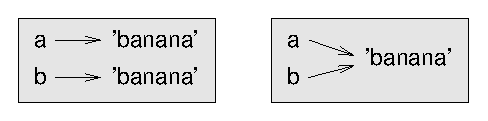
\includegraphics{figs2/list1.eps}}
\afterfig

Em um caso, {\tt a} e {\tt b} se referem a dois objetos diferentes
que tem o mesmo valor. No segundo caso, eles se referem ao mesmo objeto.
% In one case, {\tt a} and {\tt b} refer to two different objects that
% have the same value.  In the second case, they refer to the same
% object.

\index{operador}
\index{is!operador}

Para checar se duas variáveis referem-se ao mesmo objeto, você pode
utilizar o operador {\tt is}.
% To check whether two variables refer to the same object, you can
% use the {\tt is} operator.

\beforeverb
\begin{verbatim}
>>> a = 'banana'
>>> b = 'banana'
>>> a is b
True
\end{verbatim}
\afterverb
%

Neste exemplo, o Python apenas criou um objeto string,
e ambos {\tt a} e {\tt b} referem-se a ele.
% In this example, Python only created one string object,
% and both {\tt a} and {\tt b} refer to it.

Porém, quando você cria duas listas, você tem dois objetos:
% But when you create two lists, you get two objects:

\beforeverb
\begin{verbatim}
>>> a = [1, 2, 3]
>>> b = [1, 2, 3]
>>> a is b
False
\end{verbatim}
\afterverb
%

Neste caso, diríamos que as duas listas são {\bf equivalentes},
pois possuem os mesmos elementos, mas não são {\bf idênticas}, já
que não são o mesmo objeto. Se dois objetos são idênticos, eles também
são equivalentes, porém se eles são equivalentes, não são necessariamente
idênticos.
% In this case we would say that the two lists are {\bf equivalent},
% because they have the same elements, but not {\bf identical}, because
% they are not the same object.  If two objects are identical, they are
% also equivalent, but if they are equivalent, they are not necessarily
% identical.

\index{equivalência}
\index{identidade}
%\index{equivalence}
%\index{identity}

Até agora estivemos utilizando a nomenclatura ``objeto'' ou ``valor'', mas, é
mais preciso dizer que um objeto tem um valor. Se você executa 
{\tt a = [1,2,3]}, {\tt a} refere-se a um objeto lista do qual o
valor é uma sequência particular de elementos. Se outra lista tem os mesmos
elementos, diríamos que tem o mesmo valor.
% Until now, we have been using ``object'' and ``value''
% interchangeably, but it is more precise to say that an object has a
% value.  If you execute {\tt a = [1,2,3]}, {\tt a} refers to a list
% object whose value is a particular sequence of elements.  If another
% list has the same elements, we would say it has the same value.

\index{objeto}
\index{valor}
%\index{object}
%\index{value}

\section{Aliasing - Interferência entre variáveis}
%\section{Aliasing}

\index{aliasing}
\index{aliasing!referência}
%\index{aliasing}
%\index{reference!aliasing}

Se {\tt a} refere-se a um objeto e você atribui {\tt b = a},
então ambas as variáveis referem-se ao mesmo objeto:
% If {\tt a} refers to an object and you assign {\tt b = a},
% then both variables refer to the same object:

\beforeverb
\begin{verbatim}
>>> a = [1, 2, 3]
>>> b = a
>>> b is a
True
\end{verbatim}
\afterverb
%

A associação de uma variável com um objeto é chamada
{\bf referência}. Neste exemplo existem duas referências para o
mesmo objeto.
% The association of a variable with an object is called a {\bf
% reference}.  In this example, there are two references to the same
% object.

\index{referência}
%\index{reference}

Um objeto com mais de uma referência tem mais de um nome,
então dizemos que o objeto é {\bf aliased}.
% An object with more than one reference has more
% than one name, so we say that the object is {\bf aliased}.

\index{mutabilidade}

Se o objeto {\bf aliased} é mutável,
modificações feitas com um alias 
afetará as outras:

% If the aliased object is mutable, 
% changes made with one alias affect
% the other:

\beforeverb
\begin{verbatim}
>>> b[0] = 17
>>> print a
[17, 2, 3]
\end{verbatim}
\afterverb
%

Embora este comportamento possa ser útil, é passível de erro. De maneira
geral é mais seguro evitar {\bf aliasing} quando você está trabalhando com objetos mutáveis.
%Although this behavior can be useful, it is error-prone.  In general,
%it is safer to avoid aliasing when you are working with mutable
%objects.

\index{imutabilidade}
%\index{mutability}

Para objetos imutáveis como strings, {\bf aliasing} não chega a ser um problema. 
Neste exemplo:
%For immutable objects like strings, aliasing is not as much of a
%problem.  In this example:

\beforeverb
\begin{verbatim}
a = 'banana'
b = 'banana'
\end{verbatim}
\afterverb
%

Isso quase nunca faz diferença, se {\tt a} e {\tt b} fazem referência à mesma string ou não.
%it almost never makes a difference whether {\tt a} and {\tt b} refer
%to the same string or not.

\section{Argumentos de Lista}
%\section{List arguments}

\index{como argumento!lista}
\index{argumento}
\index{lista!argumento}
\index{referência}
\index{parâmetro}
%\index{list!as argument}
%\index{argument}
%\index{argument!list}
%\index{reference}
%\index{parameter}

Quando você passa uma lista para uma função, a função pega uma referência para a lista.
Se a função modifica a lista passada como argumento, o "caller" vê a mudança.
Por exemplo, \verb"delete_head" remove o primeiro elemento da lista:
%When you pass a list to a function, the function gets a reference
%to the list.
%If the function modifies a list parameter, the caller sees the change.
%For example, \verb"delete_head" removes the first element from a list:

\beforeverb
\begin{verbatim}
def delete_head(t):
    del t[0]
\end{verbatim}
\afterverb
%
Aqui está como isto é utilizado:
%Here's how it is used:

\beforeverb
\begin{verbatim}
>>> letters = ['a', 'b', 'c']
>>> delete_head(letters)
>>> print letters
['b', 'c']
\end{verbatim}
\afterverb
%

O parâmetro {\tt t} e a variável {\tt letters} são {\bf aliases} para o mesmo objeto.
%The parameter {\tt t} and the variable {\tt letters} are
%aliases for the same object.

Isso é importante para distinguir entre operações que modificam listas e operações que criam novas listas.
Por exemplo, o método {\tt append} modifica uma lista, mas o operador {\tt +} cria uma nova lista:
%It is important to distinguish between operations that
%modify lists and operations that create new lists.  For
%example, the {\tt append} method modifies a list, but the
%{\tt +} operator creates a new list:

\index{método append}
\index{append!método}
\index{concatenada!lista}
\index{lista!concatenada}
%\index{append method}
%\index{method!append}
%\index{list!concatenation}
%\index{concatenation!list}


\beforeverb
\begin{verbatim}
>>> t1 = [1, 2]
>>> t2 = t1.append(3)
>>> print t1
[1, 2, 3]
>>> print t2
None

>>> t3 = t1 + [3]
>>> print t3
[1, 2, 3]
>>> t2 is t3
False
\end{verbatim}
\afterverb

Esta diferença é importante quando você escreve funções que supostamente devem modificar listas.
Por exemplo, esta função \emph{não} deleta o início de uma lista:
%This difference is important when you write functions that
%are supposed to modify lists.  For example, this function
%\emph{does not} delete the head of a list:

\beforeverb
\begin{verbatim}
def bad_delete_head(t):
    t = t[1:]              # ERRADO!
\end{verbatim}
\afterverb

O operador de fatiamento cria uma nova lista e a atribuição faz {\tt t} se referir a isto,
porém nada disso tem efeito na lista passada como argumento.
%The slice operator creates a new list and the assignment
%makes {\tt t} refer to it, but none of that has any effect
%on the list that was passed as an argument.

\index{operador de fatiamento}
\index{fatiamento!operador}
%\index{slice operator}
%\index{operator!slice}

Uma alternativa é escrever uma função que cria e retorna uma nova lista.
Por exemplo, {\tt tail} retorna tudo, menos o primeiro elemento de uma lista: 
%An alternative is to write a function that creates and
%returns a new list.  For
%example, {\tt tail} returns all but the first
%element of a list:

\beforeverb
\begin{verbatim}
def tail(t):
    return t[1:]
\end{verbatim}
\afterverb
%

Esta função deixa a lista original inalterada.
Aqui está como isto é utilizado:
%This function leaves the original list unmodified.
%Here's how it is used:

\beforeverb
\begin{verbatim}
>>> letters = ['a', 'b', 'c']
>>> rest = tail(letters)
>>> print rest
['b', 'c']
\end{verbatim}
\afterverb

\begin{ex}

Escreva uma função chamada {\tt chop} que recebe uma lista e a modifica,
removendo o primeiro e o último elementos e retorna {\tt None}.
%Write a function called {\tt chop} that takes a list and modifies
%it, removing the first and last elements, and returns {\tt None}.

Então escreva uma função chamada {\tt middle} que recebe uma lista e retorna
uma nova lista que contenha tudo menos o primeiro e o último elementos.
%Then write a function called {\tt middle} that takes a list and
%returns a new list that contains all but the first and last
%elements.

\end{ex}

\section{Depurando}
\index{depurando}
%\section{Debugging}
%\index{debugging}

O uso descuidado de listas (e outros objetos mutáveis) 
pode levar a longas horas de depuração. Aqui estão algumas das
armadilhas mais comuns e maneiras de evitá-las.
%Careless use of lists (and other mutable objects)
%can lead to long hours of debugging.  Here are some common
%pitfalls and ways to avoid them:

\begin{enumerate}

\item Não esqueça que a maioria dos métodos de lista modificam o argumento
  e retornam {\tt None}. Isto é o oposto dos métodos de string, os quais retornam
  uma nova string e deixam o original inalterado.
%\item Don't forget that most list methods modify the argument and
%  return {\tt None}.  This is the opposite of the string methods,
%  which return a new string and leave the original alone.

Se você está acostumado a escrever código para strings assim:
%If you are used to writing string code like this:

\beforeverb
\begin{verbatim}
word = word.strip()
\end{verbatim}
\afterverb

É tentador escrever código para lista assim:
%It is tempting to write list code like this:

\beforeverb
\begin{verbatim}
t = t.sort()           # ERRADO!
\end{verbatim}
\afterverb

\index{método sort}
\index{sort!método}
%\index{sort method}
%\index{method!sort}

Por {\tt sort} retornar {\tt None}, a
próxima operação que você executar com {\tt tt} provavelmente falhará.
%Because {\tt sort} returns {\tt None}, the
%next operation you perform with {\tt t} is likely to fail.

Antes de usar métodos e operadores de lista você deveria ler a documentação com
cuidado e então testá-los no modo interativo. Os métodos e operadores que as listas
compartilham com outras sequências (como strings) são documentados em
\url{https://docs.python.org/2/library/stdtypes.html#string-methods}.
Os métodos e operadores que se aplicam apenas a sequências mutáveis são documentados
em:
\url{https://docs.python.org/2/library/stdtypes.html#mutable-sequence-types}.
%Before using list methods and operators, you should read the
%documentation carefully and then test them in interactive mode.  The
%methods and operators that lists share with other sequences (like
%strings) are documented at
%\url{https://docs.python.org/2/library/stdtypes.html#string-methods}.
%The methods and operators that only apply to mutable sequences
%are documented at
%\url{https://docs.python.org/2/library/stdtypes.html#mutable-sequence-types}.

\item Pegue um idioma e fique como ele.
\index{idioma}
%\item Pick an idiom and stick with it.
%\index{idiom}

Parte do problema com listas é que existem muitas maneiras 
de fazer as coisas. Por exemplo, para remover um elemento
de uma lista, você pode usar {\tt pop}, {\tt remove}, {\tt del},
ou mesmo atribuição de um fatiamento (slice).
%Part of the problem with lists is that there are too many
%ways to do things.  For example, to remove an element from
%a list, you can use {\tt pop}, {\tt remove}, {\tt del},
%or even a slice assignment.

Para adicionar um elemento, você pode utilizar os métodos {\tt append} 
ou o operador {\tt +}. Mas não esqueça que esses estão corretos:
%To add an element, you can use the {\tt append} method or
%the {\tt +} operator.  But don't forget that these are right: 

\beforeverb
\begin{verbatim}
t.append(x)
t = t + [x]
\end{verbatim}
\afterverb

E esses estão errados:
%And these are wrong:

\beforeverb
\begin{verbatim}
t.append([x])          # ERRADO!
t = t.append(x)        # ERRADO!
t + [x]                # ERRADO!
t = t + x              # ERRADO!
\end{verbatim}
\afterverb

Experimente cada um desses exemplos no modo interativo para ter
certeza que você entende o que eles fazem. Note que apenas o último
causa um erro de runtime; os outros três são legais, mas fazem a coisa
errada.
%Try out each of these examples in interactive mode to make sure
%you understand what they do.  Notice that only the last
%one causes a runtime error; the other three are legal, but they
%do the wrong thing.


\item Faça cópias para evitar aliasing.
%\item Make copies to avoid aliasing.

\index{copiando para evitar! aliasing}
\index{copiar!para evitar aliasing}
%\index{aliasing!copying to avoid}
%\index{copy!to avoid aliasing}

Se você quer usar um método como {\tt sort} que modifica
o argumento, mas você também precisa manter a lista original,
você pode fazer uma cópia.
%If you want to use a method like {\tt sort} that modifies
%the argument, but you need to keep the original list as
%well, you can make a copy.

\beforeverb
\begin{verbatim}
orig = t[:]
t.sort()
\end{verbatim}
\afterverb

Neste exemplo você também pode usar a função built-in {\tt sorted},
a qual retorna uma nova lista ordenada e deixa a original inalterada.
Mas, neste caso você deve evitar {\tt sorted} como um nome de variável!
%In this example you could also use the built-in function {\tt sorted},
%which returns a new, sorted list and leaves the original alone.
%But in that case you should avoid using {\tt sorted} as a variable
%name!

\item Listas, {\tt split}, e arquivos
%\item Lists, {\tt split}, and files

Quando lemos e analisamos arquivos, existem muitas oportunidades
para encontrar entradas que podem causar falhas em nosso programa,
então é uma boa ideia revisitar o padrão {\bf protetor} quando
se trata de escrever programas que leiam de um arquivo e procurem
por uma ``agulha no palheiro''.
%When we read and parse files, there are many opportunities
%to encounter input that can crash our program so it is a good 
%idea to revisit the {\bf guardian} pattern when it comes
%writing programs that read through a file 
%and look for a ``needle in the haystack''.

Vamos revisitar nosso programa que procura pelo dia da semana
nas linhas do nosso arquivo:
%Let's revisit our program that is looking for the day of the
%week on the from lines of our file:

\beforeverb
\begin{alltt}
From stephen.marquard@uct.ac.za {\bf Sat} Jan  5 09:14:16 2008
\end{alltt}
\afterverb

Já que estamos quebrando esta linha em palavras, poderíamos distribuir
isso com o uso do {\tt startswith} e simplesmente olhar a primeira palavra
da linha para determinar se estamos interessados na linha. Podemos usar {\tt continue} 
para pular linhas que não possuem ``From'' como primeira palavra:
%Since we are breaking this line into words, we could dispense
%with the use of {\tt startswith} and simply look at the 
%first word of the line to determine if we are interested
%in the line at all.  We can use {\tt continue} to skip lines
%that don't have ``From'' as the first word as follows:

\beforeverb
\begin{verbatim}
fhand = open('mbox-short.txt')
for line in fhand:
    words = line.split()
    if words[0] != 'From' : continue
    print words[2]
\end{verbatim}
\afterverb
%

Isso parece muito mais simples e nós nem mesmo precisamos fazer o
{\tt rstrip} para remover o newline ao final do arquivo.
Mas, é melhor assim?
%This looks much simpler and we don't even need to do the 
%{\tt rstrip} to remove the newline at the end of the file.
%But is it better?

\beforeverb
\begin{verbatim}
python search8.py 
Sat
Traceback (most recent call last):
  File "search8.py", line 5, in <module>
    if words[0] != 'From' : continue
IndexError: list index out of range
\end{verbatim}
\afterverb
%

Funciona de certa maneira e vemos o dia da primeira
(Sat), mas então o programa falha com um erro traceback.
O que deu errado? Que dados bagunçados causaram a falha do
nosso elegante, inteligente e Pythonico programa?
%It kind of works and we see the day from the first line
%(Sat), but then the program fails with a traceback error.
%What went wrong?  What messed-up data caused our elegant, 
%clever, and very Pythonic program to fail?

Você pode ficar olhando por um longo tempo e tentar decifrá-lo ou
pedir ajuda para alguém, porém a abordagem mais rápida e inteligente
é adicionar um {\tt print}. O melhor lugar para colocar um print é
logo antes da linha onde o programa falhou e imprimir os dados que 
parecem estar causando a falha.
%You could stare at it for a long time and puzzle through
%it or ask someone for help, but the quicker and smarter
%approach is to add a {\tt print} statement.  The best place
%to add the print statement is right before the line where
%the program failed and print out the data that seems to be causing
%the failure.

Essa abordagem deve gerar muitas linhas na saída do programa,
mas, ao menos você imediatamente terá alguma pista sobre o problema.
Então adicione um print da variável {\tt words} logo antes da linha cinco.
Nós até mesmo colocamos um prefixo: ``Debug:'' na linha, assim podemos 
manter nossa saída normal separada da saída de debug.
%Now this approach may generate a lot of lines of output, but
%at least you will immediately have some clue as to the 
%problem at hand.  So we add a print of the variable
%{\tt words} right before line five.  We even 
%add a prefix ``Debug:'' to the line so we can keep
%our regular output separate from our debug output.

\beforeverb
\begin{verbatim}
for line in fhand:
    words = line.split()
    print 'Debug:', words
    if words[0] != 'From' : continue
    print words[2]
\end{verbatim}
\afterverb
%
Quando executamos o programa, há muita saída passando pela tela,
mas ao fim vemos nossa saída de debug e um traceback, dessa forma
sabemos o que aconteceu antes do traceback.
%When we run the program, a lot of output scrolls off the screen
%but at the end, we see our debug output and the traceback so 
%we know what happened just before the traceback.

\beforeverb
\begin{verbatim}
Debug: ['X-DSPAM-Confidence:', '0.8475']
Debug: ['X-DSPAM-Probability:', '0.0000']
Debug: []
Traceback (most recent call last):
  File "search9.py", line 6, in <module>
    if words[0] != 'From' : continue
IndexError: list index out of range
\end{verbatim}
\afterverb
%

Cada linha de debug imprime uma lista de palavras que temos quando
quando dividimos a linha em palavras {\tt split}. Quando o programa
falha, a lista de palavras está vazia \verb"[]". Se abrirmos um arquivo
em um editor de texto e olharmos neste ponto, ele parecerá conforme a seguir:
%Each debug line is printing the list of words which we get
%when we {\tt split} the line into words.  When the program fails,
%the list of words is empty \verb"[]".  If we open the file in a
%text editor and look at the file, at that point it looks as follows:

\beforeverb
\begin{verbatim}
X-DSPAM-Result: Innocent
X-DSPAM-Processed: Sat Jan  5 09:14:16 2008
X-DSPAM-Confidence: 0.8475
X-DSPAM-Probability: 0.0000

Detalhes: http://source.sakaiproject.org/viewsvn/?view=rev&rev=39772
\end{verbatim}
\afterverb
%

O erro ocorre quando nosso programa encontra uma linha em branco! Claro, uma linha em
branco tem ``zero palavras''. Porque não pensamos nisso quando estávamos escrevendo o código?
Quando o código procura pela primeira palavra (\verb"word[0]") para ver se encontra ``From'',
nós então temos um erro ``index out of range''.
%The error occurs when our program encounters a blank line! Of course there
%are ``zero words'' on a blank line.  Why didn't we think of that 
%when we were writing the code?  When the code looks for the first
%word (\verb"word[0]") to check to see if it matches ``From'', 
%we get an ``index out of range'' error.

Este é claro, o lugar perfeito para adicionar algum código {\bf protetor} para
evitar a checagem da primeira palavra caso ela não exista.
Existem muitas maneiras de proteger este código; escolheremos checar
o número de palavras que temos antes de olharmos a primeira palavra:
%This of course is the perfect place to add some {\bf guardian} code 
%to avoid checking the first word if the first word is not there.
%There are many ways to protect this code; we will choose to 
%check the number of words we have before we look at the first word:

\beforeverb
\begin{verbatim}
fhand = open('mbox-short.txt')
count = 0
for line in fhand:
    words = line.split()
    # print 'Debug:', words
    if len(words) == 0 : continue
    if words[0] != 'From' : continue
    print words[2]
\end{verbatim}
\afterverb
%

Primeiramente, comentamos o print de debug ao invés de removê-lo,
para caso nossa modificação falhe, precisaremos investigar novamente.
Então adicionamos uma instrução protetora que verifica se temos zero palavras, caso positivo,
usamos {\tt continue} para pular para a próxima linha no arquivo.
%First we commented out the debug print statement instead of removing it, 
%in case our modification fails and we need to debug again.  Then we added
%a guardian statement that checks to see if we have zero words, and if so, 
%we use {\tt continue} to skip to the next line in the file.

Podemos pensar nas duas instruções {\tt continue} nos ajudando a refinar
o conjunto de linhas que são ``interessantes'' para nós e quais queremos
processar mais um pouco. Uma linha que não tenha palavras ``não é interessante''
para nós então, pulamos para a próxima linha. Uma linha que não tenha ``From''
como a sua primeira palavra não é interessante para nós, então nós a pulamos.
%We can think of the two {\tt continue} statements as helping us refine
%the set of lines which are ``interesting'' to us and which we want 
%to process some more.  A line which has no words is ``uninteresting'' to 
%us so we skip to the next line.  A line which does not have ``From''
%as its first word is uninteresting to us so we skip it.

O programa, da forma como foi modificado, executa com sucesso, então talvez esteja correto.
Nossa instrução protetora assegurará que {\tt words[0]} nunca falhará,
mas talvez isso não seja o suficiente. Quando estamos programando, devemos sempre estar pensando,
``O que pode dar errado?''
%The program as modified runs successfully, so perhaps it is correct.  Our
%guardian statement does make sure that the {\tt words[0]} will never fail, 
%but perhaps it is not enough.  When we are programming, we must always be 
%thinking, ``What might go wrong?''

\begin{ex}
Descubra qual linha do programa acima, ainda não está corretamente protegida.
Veja se você pode construir um arquivo de texto que causará falha no programa e
então modifique o programa para que então a linha esteja corretamente protegida e
teste para ter certeza de que o programa processará o novo arquivo de texto.
\end{ex}
%\begin{ex}
%Figure out which line of the above program is still not properly guarded.
%See if you can construct a text file which causes the program to fail
%and then modify the program so that the line is properly guarded and 
%test it to make sure it handles your new text file.
%\end{ex}

\begin{ex}
Reescreva o código protetor, no exemplo acima, sem as duas instruções {\tt if}. Ao invés
disso, use uma expressão lógica combinada com o operador lógico {\tt and} com apenas uma
instrução {\tt if}.
\end{ex}
%\begin{ex}
%Rewrite the guardian code in the above example without two
%{\tt if} statements.  Instead, use a compound logical expression using the
%{\tt and} logical operator with a single {\tt if} statement.
%\end{ex}

\end{enumerate}

\section{Glossário}
%\section{Glossary}

\begin{description}

\item[aliasing:] Uma circunstância onde duas ou mais variáveis, referem-se ao mesmo objeto.
\index{aliasing}
%\item[aliasing:] A circumstance where two or more variables refer to the same
%object.
%\index{aliasing}

\item[delimitador:] Um caractere (ou string) usada para indicar onde uma string deve ser dividida.
\index{delimitador}
%\item[delimiter:] A character or string used to indicate where a
%string should be split.
%\index{delimiter}

\item[elemento:] Um dos valores em uma lista (ou outra sequência);
também chamado de itens.
\index{elemento}
%\item[element:] One of the values in a list (or other sequence);
%also called items.
%\index{element}

\item[equivalente:] Ter os mesmos valores.
\index{equivalente}
%\item[equivalent:] Having the same value.
%\index{equivalent}

\item[index:] Um valor inteiro que indica um elemento em uma lista.
\index{index}

\item[idêntico:] É o mesmo objeto (o que indica equivalência).
\index{idêntico}
%\item[index:] An integer value that indicates an element in a list.
%\index{index}

\item[lista:] Uma sequência de valores.
\index{lista}
%\item[identical:] Being the same object (which implies equivalence).
%\index{identical}

\item[percorrer lista:] Acesso sequencial a cada elemento de uma lista.
\index{lista!percorrer}
%\item[list:] A sequence of values.
%\index{list}

\item[lista aninhada:] Uma lista que é um elemento de outra lista.
\index{lista aninhada}
%\item[list traversal:] The sequential accessing of each element in a list.
%\index{list!traversal}

\item[objeto:] Algo a que uma variável pode se referir. Uma objeto tem um tipo e valor.
\index{objeto}
%\item[nested list:] A list that is an element of another list.
%\index{nested list}

\item[referência:] Uma associação entre uma variável e seu valor.
\index{referência}
%\item[object:] Something a variable can refer to.  An object
%has a type and a value.
%\index{object}

\end{description}

\section{Exercícios}

\begin{ex}
Faça o download de uma cópia do arquivo em
%Download a copy of the file from 
\url{www.py4inf.com/code/romeo.txt}
\index{Romeo and Juliet}

Escreva um programa para abrir o arquivo {\tt romeo.txt}
e ler linha por linha. Para cada linha, divida a linha em uma lista
de palavras usando a função {\tt split}.
%Write a program to open the file {\tt romeo.txt} and read it
%line by line.  For each line, split the line into  a list of 
%words using the {\tt split} function.

Para cada palavra, verifique se a palavra já está em uma lista.
Se a palavra não está na lista, adicione à lista.
%For each word, check to see if the word is already in a list.  
%If the word is not in the list, add it to the list.  

Quando o programa completar, ordene e imprima as palavras resultantes
em ordem alfabética.
%When the program completes, sort and print the resulting words
%in alphabetical order.

\begin{verbatim}
Enter file: romeo.txt
['Arise', 'But', 'It', 'Juliet', 'Who', 'already', 
'and', 'breaks', 'east', 'envious', 'fair', 'grief', 
'is', 'kill', 'light', 'moon', 'pale', 'sick', 'soft', 
'sun', 'the', 'through', 'what', 'window', 
'with', 'yonder']
\end{verbatim}
\end{ex}

\begin{ex}
Escreva um programa para ler os dados do mail box e quando você achar
uma linha que inicie com ``From'', você dividirá a linha em palavras 
usando a função {\tt split}. Estamos interessados em quem enviou a mensagem,
que é a segunda palavra na linha do From.
%Write a program to read through the mail box data and when you find 
%line that starts with ``From'', you will split the line into 
%words using the {\tt split} function. We are interested in 
%who sent the message, which is the second word on the From line.

{\tt From stephen.marquard@uct.ac.za Sat Jan  5 09:14:16 2008 }

Você irá analisar a linha do From, imprimir a segunda palavra
para cada linha com From, então você também contará o número de 
linhas com From ( e não From:) e imprimirá e calculará ao final.
%You will parse the From line and print out the second word for 
%each From line, then you will also count the number of 
%From (not From:) lines and print out a count at the end.

Este é um bom exemplo de saída com algumas linhas removidas:
%This is a good sample output with a few lines removed:

\beforeverb
\begin{verbatim}
python fromcount.py 
Enter a file name: mbox-short.txt
stephen.marquard@uct.ac.za
louis@media.berkeley.edu
zqian@umich.edu

[...Parte da saída removida...]

ray@media.berkeley.edu
cwen@iupui.edu
cwen@iupui.edu
cwen@iupui.edu
Existiam 27 linhas no arquivos onde From era a primeira palavra
\end{verbatim}
\afterverb
%
\end{ex}

\begin{ex}

Reescreva o programa que leva o usuário para uma lista de 
números e imprime o máximo e o mínimo para os números no fim 
quando o usuário digita ``done''. Escreva um programa para armazenar
em uma lista, os números que o usuário digitar e use as funções
{\tt max()} e {\tt min()} para calcular o máximo e o mínimo ao fim
do loop.
%Rewrite the program that prompts the user for a list of 
%numbers and prints out the maximum and minimum of the
%numbers at the end when the user enters ``done''.  Write
%the program to store the numbers the user enters in a list
%and use the {\tt max()} and {\tt min()} functions to 
%compute the maximum and minimum numbers after the 
%loop completes.

\beforeverb
\begin{verbatim}
Digite um número: 6
Digite um número: 2
Digite um número: 9
Digite um número: 3
Digite um número: 5
Digite um número: done
Maximum: 9.0
Minimum: 2.0
\end{verbatim}
\afterverb
%

\end{ex}
% LaTeX source for ``Python for Informatics: Exploring Information''
% Copyright (c)  2010-  Charles R. Severance, All Rights Reserved

\chapter{Dicionários}
%\chapter{Dictionaries}
\index{dicionário}
% \index{dictionary}

\index{dicionário}
% \index{dictionary}
\index{tipo!dict}
% \index{type!dict}
\index{chave}
% \index{key}
\index{par chave-valor}
% \index{key-value pair}
\index{índice}
% \index{index}


Um {\bf dicionário} é como uma lista, porém mais abrangente. Em uma lista,
os índices devem ser valores inteiros; em um dicionário,
os índices podem ser de qualquer tipo (praticamente).
% A {\bf dictionary} is like a list, but more general.  In a list,
% the index positions have to be integers; in a dictionary,
% the indices can be (almost) any type.

Pode-se considerar um dicionário como um mapeamento entre um conjunto de
índices (chamados de {\bf chaves}) e um conjunto de valores. Cada chave é
mapeada a um valor. A associação entre uma chave e um valor é chamada de
{\bf par chave-valor} ou também como um {\bf item}.
% You can think of a dictionary as a mapping between a set of indices
% (which are called {\bf keys}) and a set of values.  Each key maps to a
% value.  The association of a key and a value is called a {\bf
%   key-value pair} or sometimes an {\bf item}.

Como exemplo, construiremos um dicionário que mapeia palavras inglesas para
palavras em espanhol, portanto chaves e valores são strings.
% As an example, we'll build a dictionary that maps from English
% to Spanish words, so the keys and the values are all strings.

A função {\tt dict} cria um novo dicionário sem itens. Pelo fato de {\tt dict} ser o
nome de uma função padrão da linguagem, esse termo não pode ser usado como nome de variável.
% The function {\tt dict} creates a new dictionary with no items.
% Because {\tt dict} is the name of a built-in function, you
% should avoid using it as a variable name.

\index{funcão dict}
% \index{dict function}
\index{função!dict}
% \index{function!dict}

\beforeverb
\begin{verbatim}
>>> eng2sp = dict()
>>> print eng2sp
{}
\end{verbatim}
\afterverb
%

Os caracteres chaves, \verb"{}", representam um dicionário vazio.
Colchetes podem ser utilizados para adicionar itens ao dicionário:
% The curly brackets, \verb"{}", represent an empty dictionary.
% To add items to the dictionary, you can use square brackets:

\index{caractere chave}
% \index{squiggly bracket}
\index{caractere!chave}
% \index{bracket!squiggly}

\beforeverb
\begin{verbatim}
>>> eng2sp['one'] = 'uno'
\end{verbatim}
\afterverb
%

Esta linha cria um item que mapeia da chave {\tt 'one'}
para o valor \verb"'uno'". Se exibirmos o dicionário novamente, veremos
um par chave-valor com o caractere dois-pontos entre a chave e o valor:
% This line creates an item that maps from the key
% {\tt 'one'} to the value \verb"'uno'".  If we print the
% dictionary again, we see a key-value pair with a colon
% between the key and value:

\beforeverb
\begin{verbatim}
>>> print eng2sp
{'one': 'uno'}
\end{verbatim}
\afterverb
%

Esse formato de saída também é um formato de entrada. Por exemplo,
pode-se criar um novo dicionário com três itens:
% This output format is also an input format.  For example,
% you can create a new dictionary with three items:

\beforeverb
\begin{verbatim}
>>> eng2sp = {'one': 'uno', 'two': 'dos', 'three': 'tres'}
\end{verbatim}
\afterverb
%

Mas se exibirmos {\tt eng2sp}, podemos nos surpreender:
% But if you print {\tt eng2sp}, you might be surprised:

\beforeverb
\begin{verbatim}
>>> print eng2sp
{'one': 'uno', 'three': 'tres', 'two': 'dos'}
\end{verbatim}
\afterverb
%

A ordem dos pares chave-valor não é a mesma. De fato, se esse mesmo
exemplo for executado em outro computador, um resultado diferente pode
ser obtido. Em linhas gerais, a ordem dos elementos em um dicionário
é imprevisível.
% The order of the key-value pairs is not the same.  In fact, if
% you type the same example on your computer, you might get a
% different result.  In general, the order of items in
% a dictionary is unpredictable.

Entretanto, isso não é um problema, uma vez que os elementos de um dicionário
nunca são indexados por índices inteiros. Ao invés disso, usa-se as chaves para
se buscar os valores correspondentes:
% But that's not a problem because
% the elements of a dictionary are never indexed with integer indices.
% Instead, you use the keys to look up the corresponding values:

\beforeverb
\begin{verbatim}
>>> print eng2sp['two']
'dos'
\end{verbatim}
\afterverb
%

A ordem dos itens não importa, já que a chave {\tt 'two'} sempre é mapeada ao valor \verb"'dos'".
% The key {\tt 'two'} always maps to the value \verb"'dos'" so the order
% of the items doesn't matter.

Se a chave não está no dicionário, uma exceção é levantada:
% If the key isn't in the dictionary, you get an exception:

\index{exceção!KeyError}
% \index{exception!KeyError}
\index{KeyError}

\beforeverb
\begin{verbatim}
>>> print eng2sp['four']
KeyError: 'four'
\end{verbatim}
\afterverb
%

A função {\tt len} também pode ser usada em dicionários; ela devolve
o número de pares chave-valor:
% The {\tt len} function works on dictionaries; it returns the
% number of key-value pairs:

\index{função len}
% \index{len function}
\index{função!len}
% \index{function!len}

\beforeverb
\begin{verbatim}
>>> len(eng2sp)
3
\end{verbatim}
\afterverb
%

Pode-se utilizar o operador {\tt in} para se verificar se algo está representado
como uma \emph{chave} no dicionário (não serve para verificar diretamente
a presença de um valor).
% The {\tt in} operator works on dictionaries; it tells you whether
% something appears as a \emph{key} in the dictionary (appearing
% as a value is not good enough).

\index{membro!dictionário}
% \index{membership!dictionary}
\index{operador in}
% \index{in operator}
\index{operador!in}
% \index{operator!in}

\beforeverb
\begin{verbatim}
>>> 'one' in eng2sp
True
>>> 'uno' in eng2sp
False
\end{verbatim}
\afterverb
%

Para verificar se algo está representado como um valor no dicionário, pode-se usar o método {\tt values}, o qual devolve os valores como uma lista e, desse
modo, o operador {\tt in} pode ser usado:
% To see whether something appears as a value in a dictionary, you
% can use the method {\tt values}, which returns the values as
% a list, and then use the {\tt in} operator:

\index{método values}
% \index{values method}
\index{método!values}
% \index{method!values}

\beforeverb
\begin{verbatim}
>>> vals = eng2sp.values()
>>> 'uno' in vals
True
\end{verbatim}
\afterverb
%

O operador {\tt in} usa algoritmos diferentes para listas e dicionários. Para
listas é usado um algoritmo de busca linear. Conforme o tamanho da lista aumenta, o tempo de busca aumenta de maneira diretamente proporcional ao tamanho da lista.
Para dicionários, Python usa um algoritmo chamado {\bf tabela de hash}, a qual possui uma propriedade notável---o operador {\tt in} consume a mesma quantidade de tempo para se realizar a busca independente do número de itens existente no dicionário. Aqui não será explicado o porquê das funções de hash serem tão mágicas, mas informações adicionais sobre esse assunto podem ser lidas em \url{pt.wikipedia.org/wiki/Tabela_de_dispersão}.
% The {\tt in} operator uses different algorithms for lists and
% dictionaries.  For lists, it uses a linear search algorithm.
% As the list gets longer, the search time gets
% longer in direct proportion to the length of the list.
% For dictionaries, Python uses an
% algorithm called a {\bf hash table} that has a remarkable property---the
% {\tt in} operator takes about the same amount of time no matter how
% many items there are in a dictionary.  I won't explain
% why hash functions are so magical,
% but you can read more about it at
% \url{wikipedia.org/wiki/Hash_table}.

\index{tabela hash}
% \index{hash table}

\begin{ex}
\label{wordlist2}

\index{definir membro}
% \index{set membership}
\index{membro!definir}
% \index{membership!set}

Escreva um programa que leia as palavras do arquivo {\tt words.txt} e armazene-as como chaves em um dicionário. Os valores não importam. Então, use o operador {\tt in} como uma maneira rápida de verificar se uma string está no dicionário.
% Write a program that reads the words in {\tt words.txt} and
% stores them as keys in a dictionary.  It doesn't matter what the
% values are.  Then you can use the {\tt in} operator
% as a fast way to check whether a string is in
% the dictionary.

\end{ex}

\section{Dicionário como um conjunto de contagens}
%\section{Dictionary as a set of counters}
\label{histogram}

\index{contador}
% \index{counter}

Suponha que dada uma string deseja-se saber quantas vezes aparece cada letra. Há várias maneiras para que isso seja feito:
% Suppose you are given a string and you want to count how many
% times each letter appears.  There are several ways you could do it:

\begin{enumerate}

\item Poderiam ser criadas 26 variáveis, cada uma contendo uma letra do alfabeto. Então, a string poderia ser travessada e, para cada caractere, seria incrementado o contador correspondente, provavelmente utilizando-se operadores condicionais encadeado.
% \item You could create 26 variables, one for each letter of the
% alphabet.  Then you could traverse the string and, for each
% character, increment the corresponding counter, probably using
% a chained conditional.

\item Poderia ser criada uma lista com 26 elementos. Assim, cada caractere poderia ser convertido em um número (usando a função embutida {\tt ord}), o qual seria usado como um índice na lista, e se incrementaria o contador apropriado.
% \item You could create a list with 26 elements.  Then you could
% convert each character to a number (using the built-in function
% {\tt ord}), use the number as an index into the list, and increment
% the appropriate counter.

\item Poderia ser criado um dicionário, onde os caracteres são as chaves e os valores são as contagens correspondentes. Ao se encontrar um caractere pela primeira vez, um item é adicionado ao dicionário. Em seguida, o valor de um dado item seria incrementado.
% \item You could create a dictionary with characters as keys
% and counters as the corresponding values.  The first time you
% see a character, you would add an item to the dictionary.  After
% that you would increment the value of an existing item.

\end{enumerate}

Essas opções realizam a mesma computação, porém cada uma a implementa de um modo diferente.
% Each of these options performs the same computation, but each
% of them implements that computation in a different way.

\index{implementação}
% \index{implementation}

Uma {\bf implementação} é um modo de se executar uma computação; algumas implementações são melhores do que outras. Por exemplo, uma das vantagens de se utilizar a implementação com dicionário é que não há a necessidade de se saber de antemão quais letras aparecem na string, sendo que as letras serão adicionadas ao dicionário conforme for demandado.
% An {\bf implementation} is a way of performing a computation;
% some implementations are better than others.  For example,
% an advantage of the dictionary implementation is that we don't
% have to know ahead of time which letters appear in the string
% and we only have to make room for the letters that do appear.

Eis como o código ficaria:
%Here is what the code might look like:

\beforeverb
\begin{verbatim}
word = 'brontosaurus'
d = dict()
for c in word:
    if c not in d:
        d[c] = 1
    else:
        d[c] = d[c] + 1
print d
\end{verbatim}
\afterverb
%

De fato está sendo construído um {\bf histograma}, que é um termo estatístico para um conjunto de contagens (ou frequências).
% We are effectively computing a {\bf histogram}, which is a statistical
% term for a set of counters (or frequencies).

\index{histograma}
% \index{histogram}
\index{frequência}
% \index{frequency}
\index{travessia}
% \index{traversal}

O laço {\tt for} caminha por toda a string. Em cada iteração, se o caractere {\tt c} não está no dicionário, cria-se um novo item com chave {\tt c} e valor inicial 1 (já que essa letra foi encontrada um vez). Se {\tt c} já está no dicionário, o valor {\tt d[c]} é incrementado.
% The {\tt for} loop traverses
% the string.  Each time through the loop, if the character {\tt c} is
% not in the dictionary, we create a new item with key {\tt c} and the
% initial value 1 (since we have seen this letter once).  If {\tt c} is
% already in the dictionary we increment {\tt d[c]}.

\index{histograma}
% \index{histogram}

Eis a saída do programa:
%Here's the output of the program:

\beforeverb
\begin{verbatim}
{'a': 1, 'b': 1, 'o': 2, 'n': 1, 's': 2, 'r': 2, 'u': 2, 't': 1}
\end{verbatim}
\afterverb
%

O histograma indica que as letras {\tt 'a'} e \verb"'b'" aparecem uma vez; \verb"'o'" aparece duas vezes, e assim por diante.
% The histogram indicates that the letters {\tt 'a'} and \verb"'b'"
% appear once; \verb"'o'" appears twice, and so on.

\index{método get}
% \index{get method}
\index{método!get}
% \index{method!get}

Dicionários têm um método chamado {\tt get}, que recebe como argumento uma chave e um valor padrão. Se a chave se encontra no dicionário, {\tt get} devolve o valor correspondente; caso contrário, devolve o valor padrão. Por exemplo:
% Dictionaries have a method called {\tt get} that takes a key
% and a default value.  If the key appears in the dictionary,
% {\tt get} returns the corresponding value; otherwise it returns
% the default value.  For example:

\beforeverb
\begin{verbatim}
>>> counts = { 'chuck' : 1 , 'annie' : 42, 'jan': 100}
>>> print counts.get('jan', 0)
100
>>> print counts.get('tim', 0)
0
\end{verbatim}
\afterverb
%

O método {\tt get} pode ser usado para escrever o histograma de maneira mais concisa.
Pelo fato de {\tt get} automaticamente lidar com a ausência de uma chave no dicionário, quatro linhas de código podem ser reduzidas para uma e o bloco {\tt if} pode ser removido.
% We can use {\tt get} to write our histogram loop more concisely.
% Because the {\tt get} method automatically handles the case where a key
% is not in a dictionary, we can reduce four lines down to one
% and eliminate the {\tt if} statement.

\beforeverb
\begin{verbatim}
word = 'brontosaurus'
d = dict()
for c in word:
    d[c] = d.get(c,0) + 1
print d
\end{verbatim}
\afterverb
%

O uso do método {\tt get} para simplificar esse laço de contagem é um ``idiomatismo'' comum em Python e será usado diversas vezes no decorrer do livro. Desse modo, vale a pena dedicar um tempo e comparar o laço usando {\tt if} e o operador {\tt in} com o laço usando o método {\tt get}. Eles fazem exatamente a mesma coisa, mas o segundo é mais sucinto.
% The use of the {\tt get} method to simplify this counting loop
% ends up being a very commonly used ``idiom'' in Python and
% we will use it many times in the rest of the book.   So you should
% take a moment and compare the loop using the {\tt if} statement
% and {\tt in} operator with the loop using the {\tt get} method.
% They do exactly the same thing, but one is more succinct.
\index{idiomatismo}
% \index{idiom}

\section{Dicionários e arquivos}
%\section{Dictionaries and files}

Um dos usos comuns de dicionários é na contagem da ocorrência de palavras em arquivos de texto.
Comecemos com um arquivo muito simples contendo palavras extraídas de \emph{Romeu e Julieta}.
% One of the common uses of a dictionary is to count the occurrence
% of words in a file with some written text.
% Let's start with a very simple file of
% words taken from the text of \emph{Romeo and Juliet}.

Para os primeiros exemplos, usaremos uma versão mais curta e simplificada do texto, sem pontuações. Em seguida, trabalharemos com o texto da cena com as pontuações incluídas.
% For the first set of examples, we will use a shortened and simplified version
% of the text with no punctuation.  Later we will work with the text of the
% scene with punctuation included.

\beforeverb
\begin{verbatim}
But soft what light through yonder window breaks
It is the east and Juliet is the sun
Arise fair sun and kill the envious moon
Who is already sick and pale with grief
\end{verbatim}
\afterverb
%
Escreveremos um programa em Python, que lerá as linhas do arquivo, transformará cada linha em uma lista de palavras e, então, iterará sobre cada palavra na linha contando-a usando um dicionário.
% We will write a Python program to read through the lines of the file,
% break each line into a list of words, and then loop through each
% of the words in the line and count each word using a dictionary.

\index{laços aninhados}
% \index{nested loops}
\index{laço!aninhado}
% \index{loop!nested}
Veremos que temos dois laços {\tt for}. O laço externo lê as linhas do arquivo e o interno percorre cada palavra de uma linha em particular. Este é um exemplo de um padrão chamado {\bf laços aninhados} porque um dos laços é \emph{externo} e o outro é \emph{interno}.
% You will see that we have two {\tt for} loops.  The outer loop is reading the
% lines of the file and the inner loop is iterating through each
% of the words on that particular line.  This is an example
% of a pattern called {\bf nested loops} because one of the loops
% is the \emph{outer} loop and the other loop is the \emph{inner}
% loop.

Pelo fato do laço interno executar todas suas iterações para cada uma que o laço externo faz, diz-se que o laço interno itera ``mais rapidamente'' ao passo que o externo itera mais lentamente.
% Because the inner loop executes all of its iterations each time
% the outer loop makes a single iteration, we think of the inner
% loop as iterating ``more quickly'' and the outer loop as iterating
% more slowly.

\index{Romeu e Julieta}
% \index{Romeo and Juliet}
A combinação dos laços aninhados garante que contaremos todas as palavra de todas as linhas do arquivo de entrada.
% The combination of the two nested loops ensures that we will count
% every word on every line of the input file.

\beforeverb
\begin{verbatim}
fname = raw_input('Enter the file name: ')
try:
    fhand = open(fname)
except:
    print 'File cannot be opened:', fname
    exit()

counts = dict()
for line in fhand:
    words = line.split()
    for word in words:
        if word not in counts:
            counts[word] = 1
        else:
            counts[word] += 1

print counts
\end{verbatim}
\afterverb
%
Quando rodamos o programa, vemos o resultado bruto das contagens de modo não sorteado.
(o arquivo {\tt romeo.txt} está disponível em \url{www.py4inf.com/code/romeo.txt})
% When we run the program, we see a raw dump of all of the counts in unsorted
% hash order.
% (the {\tt romeo.txt} file is available at
% \url{www.py4inf.com/code/romeo.txt})

\beforeverb
\begin{verbatim}
python count1.py
Enter the file name: romeo.txt
{'and': 3, 'envious': 1, 'already': 1, 'fair': 1,
'is': 3, 'through': 1, 'pale': 1, 'yonder': 1,
'what': 1, 'sun': 2, 'Who': 1, 'But': 1, 'moon': 1,
'window': 1, 'sick': 1, 'east': 1, 'breaks': 1,
'grief': 1, 'with': 1, 'light': 1, 'It': 1, 'Arise': 1,
'kill': 1, 'the': 3, 'soft': 1, 'Juliet': 1}
\end{verbatim}
\afterverb
%
É um tanto quanto inconveniente procurar visualmente em um dicionário por palavras mais comuns e suas contagens. Desse modo, precisamos adicionar mais código Python para obter um resultado que seja mais útil.
% It is a bit inconvenient to look through the dictionary to find the
% most common words and their counts, so we need to add some more
% Python code to get us the output that will be more helpful.

\section{Laços de repetição e dicionário}

\index{dicionário!laço de repetição com}
% \index{dictionary!looping with}
\index{laço de repetição!com dicionários}
% \index{looping!with dictionaries}
\index{travessia}
% \index{traversal}

Se um dicionário for usado como a sequência em um bloco {\tt for}, esse iterará sobre as chaves do dicionário. Este laço exibe cada chave e o valor correspondente:
% If you use a dictionary as the sequence
% in a {\tt for} statement, it traverses
% the keys of the dictionary.  This loop
% prints each key and the corresponding value:

\beforeverb
\begin{verbatim}
counts = { 'chuck' : 1 , 'annie' : 42, 'jan': 100}
for key in counts:
    print key, counts[key]
\end{verbatim}
\afterverb
%
Que resulta em:
% Here's what the output looks like:

\beforeverb
\begin{verbatim}
jan 100
chuck 1
annie 42
\end{verbatim}
\afterverb
%
Mais uma vez, as chaves não respeitam nenhum tipo de ordenamento.
% Again, the keys are in no particular order.

\index{estilo}
% \index{idiom}
Podemos usar este padrão para implementar os diferentes estilos de laço que foram descritos anteriormente. Por exemplo, se quiséssemos encontrar todas as entradas em um dicionário com valor acima de dez, poderíamos escrever o seguinte código:
% We can use this pattern to implement the various loop idioms
% that we have described earlier.  For example if we wanted
% to find all the entries in a dictionary with a value
% above ten, we could write the following code:

\beforeverb
\begin{verbatim}
counts = { 'chuck' : 1 , 'annie' : 42, 'jan': 100}
for key in counts:
    if counts[key] > 10 :
        print key, counts[key]
\end{verbatim}
\afterverb
%
O laço {\tt for} itera pelas {\em chaves} do dicionário, então devemos usar o operador de índice para obter o {\em valor} correspondente para cada chave.
Eis o resultado da execução:
% The {\tt for} loop iterates through the
% {\em keys} of the dictionary, so we must
% use the index operator to retrieve the
% corresponding {\em value}
% for each key.
% Here's what the output looks like:

\beforeverb
\begin{verbatim}
jan 100
annie 42
\end{verbatim}
\afterverb
%
Vemos apenas as entradas com valor acima de dez.
% We see only the entries with a value above 10.

\index{método keys}
% \index{keys method}
\index{método!keys}
% \index{method!keys}

Para exibir as chaves em ordem alfabética, deve-se gerar uma lista das chaves do dicionário por meio do método {\tt keys}, disponível em objetos dicionário, e então ordenar essa lista. Em seguida, itera-se pela lista ordenada, procurando cada chave e exibindo os pares chave-valor de modo ordenado, como em:
% If you want to print the keys in alphabetical order, you first
% make a list of the keys in the dictionary using the
% {\tt keys} method available in dictionary objects,
% and then sort that list
% and loop through the sorted list, looking up each
% key and printing out key-value pairs in sorted order
% as follows:

\beforeverb
\begin{verbatim}
counts = { 'chuck' : 1 , 'annie' : 42, 'jan': 100}
lst = counts.keys()
print lst
lst.sort()
for key in lst:
    print key, counts[key]
\end{verbatim}
\afterverb
%
O que gera a seguinte saída:
% Here's what the output looks like:

\beforeverb
\begin{verbatim}
['jan', 'chuck', 'annie']
annie 42
chuck 1
jan 100
\end{verbatim}
\afterverb
%
Primeiramente, pode-se ver a lista não ordenada das chaves, obtida pelo método {\tt keys}. Em seguida, vemos os pares chave-valor gerados no laço {\tt for}.
% First you see the list of keys in unsorted order that
% we get from the {\tt keys} method.  Then we see the key-value
% pairs in order from the {\tt for} loop.

\section{Processamento avançado de texto}
%\section{Advanced text parsing}

\index{Romeu e Julieta}
%\index{Romeo and Juliet}

No exemplo acima, no qual usamos o arquivo {\tt romeo.txt}, todas as pontuações foram removidas para tornar o texto o mais simples possível. O texto original possui muitas pontuações, como mostrado abaixo.
% In the above example using the file {\tt romeo.txt},
% we made the file as simple as possible by removing
% all punctuation by hand.  The actual text
% has lots of punctuation, as shown below.

\beforeverb
\begin{verbatim}
But, soft! what light through yonder window breaks?
It is the east, and Juliet is the sun.
Arise, fair sun, and kill the envious moon,
Who is already sick and pale with grief,
\end{verbatim}
\afterverb
%
Uma vez que a função do Python {\tt split} procura por espaços e trata palavras como tokens separados por espaços, as palavras ``soft!'' e ``soft'' seriam tratadas como \emph{diferentes} e seriam criadas entradas separadas no dicionário para cada uma delas.
% Since the Python {\tt split} function looks for spaces and
% treats words as tokens separated by spaces, we would treat the
% words ``soft!'' and ``soft'' as \emph{different} words and create
% a separate dictionary entry for each word.

Além disso, como o arquivos possui letras capitalizadas, as palavras ``who'' e ``Who'' seriam tratadas como diferentes e teriam contagens diferentes.
% Also since the file has capitalization, we would treat
% ``who'' and ``Who'' as different words with different
% counts.

Podemos solucionar ambos os problemas usando os métodos de string {\tt lower}, {\tt punctuation} e {\tt translate}. Dentre esses três o método {\tt translate} é o mais complexo. Eis a documentação para {\tt translate}:
% We can solve both these problems by using the string
% methods {\tt lower}, {\tt punctuation}, and {\tt translate}.  The
% {\tt translate} is the most subtle of the methods.
% Here is the documentation for {\tt translate}:

\verb"string.translate(s, table[, deletechars])"

\emph{Deleta todos os caracteres de s que estão em deletechars (se presente) e traduz os caracteres usando table, que deve ser uma string com o comprimento de 256 caracteres fornecendo a tradução para cada valor de caractere, indexado pelo sua posição. Se table é None, então apenas a deleção de caracteres é realizada.}
% \emph{Delete all characters from s that are in deletechars (if present),
% and then translate the characters using table, which must
% be a 256-character string giving the translation for each
% character value, indexed by its ordinal. If table is None,
% then only the character deletion step is performed.}

Não iremos especificar o parâmetro {\tt table}, mas iremos usar {\tt deletechars} para deletar todas as pontuações. Iremos utilizar a lista de caracteres que o próprio Python considera como ``pontuação'':
% We will not specify the {\tt table} but we will use
% the {\tt deletechars} parameter to delete all of the punctuation.
% We will even let Python tell us the list of characters
% that it considers ``punctuation'':

\beforeverb
\begin{verbatim}
>>> import string
>>> string.punctuation
'!"#$%&\'()*+,-./:;<=>?@[\\]^_`{|}~'
\end{verbatim}
\afterverb
%
Faremos a seguinte modificação em nosso programa:
% We make the following modifications to our program:

\beforeverb
\begin{verbatim}
import string                                          # New Code

fname = raw_input('Enter the file name: ')
try:
    fhand = open(fname)
except:
    print 'File cannot be opened:', fname
    exit()

counts = dict()
for line in fhand:
    line = line.translate(None, string.punctuation)    # New Code
    line = line.lower()                                # New Code
    words = line.split()
    for word in words:
        if word not in counts:
            counts[word] = 1
        else:
            counts[word] += 1

print counts
\end{verbatim}
\afterverb
%
O programa se manteve praticamente o mesmo,com a exceção de que usamos {\tt translate} para remover todas as pontuações e {\tt lower} para tornar a linha em caixa baixa.
Note que para Python 2.5 e versões anteriores, {\tt translate} não aceita {\tt None} como primeiro parâmetro. Então, use este código para chamar translate:
% We use {\tt translate} to remove all punctuation and {\tt lower} to
% force the line to lowercase.  Otherwise the program is unchanged.
% Note that for Python 2.5 and earlier, {\tt translate} does not
% accept {\tt None} as the first parameter so use this code instead
% for the translate call:

% OBSERVAÇÂO: Na versão original falta fechar o parênteses após 'punctuation'
\beforeverb
\begin{verbatim}
print a.translate(string.maketrans(' ',' '), string.punctuation)
\end{verbatim}
\afterverb
% \beforeverb
% \begin{verbatim}
% print a.translate(string.maketrans(' ',' '), string.punctuation
% \end{verbatim}
% \afterverb
%
Parte de aprender a ``Arte do Python'' ou ``Pensar pythonicamente'' está em
perceber que Python geralmente tem capacidades embutidas para analisar muitos
dados de problemas comuns. No decorrer do tempo, vê-se exemplos de código e
documentação suficientes para se saber onde procurar para ver se alguém já escreveu alguma coisa que faça seu trabalho mais fácil.
% Part of learning the ``Art of Python'' or ``Thinking Pythonically''
% is realizing that Python
% often has built-in capabilities for many common data analysis
% problems.  Over time, you will see enough example code and read
% enough of the documentation to know where to look to see if someone
% has already written something that makes your job much easier.

A seguir esté um versão abreviada da saída:
% The following is an abbreviated version of the output:

\beforeverb
\begin{verbatim}
Enter the file name: romeo-full.txt
{'swearst': 1, 'all': 6, 'afeard': 1, 'leave': 2, 'these': 2,
'kinsmen': 2, 'what': 11, 'thinkst': 1, 'love': 24, 'cloak': 1,
a': 24, 'orchard': 2, 'light': 5, 'lovers': 2, 'romeo': 40,
'maiden': 1, 'whiteupturned': 1, 'juliet': 32, 'gentleman': 1,
'it': 22, 'leans': 1, 'canst': 1, 'having': 1, ...}
\end{verbatim}
\afterverb
%
Buscar informações nessa saída ainda é difícil e podemos usar Python para nos fornecer exatamente o que estamos procurando; contudo, para tanto, precisamos aprender sobre as {\bf tuplas} do Python. Retornaremos a esse exemplo uma vez que aprendermos sobre tuplas.
% Looking through this output is still unwieldy and we can use
% Python to give us exactly what we are looking for, but to do
% so, we need to learn about Python {\bf tuples}.  We
% will pick up this example once we learn about tuples.

\section{Depuração}
% \section{Debugging}
\index{depuração}
% \index{debugging}

Conforme se trabalha com conjuntos de dados maiores, pode ser difícil de depurá-los por exibição e checagem à mão. Eis algumas sugestões para depuração de conjuntos de dados grandes:
% As you work with bigger datasets it can become unwieldy to
% debug by printing and checking data by hand.  Here are some
% suggestions for debugging large datasets:

\begin{description}

\item[Reduza a entrada:] Se possível, reduza o tamanho do conjunto de dados.
Por exemplo, se o programa lê um arquivo de texto, comece com apenas 10 linhas,
ou com o menor exemplo que pode ser construído. Pode-se ainda editar os próprios arquivos, ou (melhor) modificar o programa de tal modo a ler apenas as {\tt n} linhas.
% \item[Scale down the input:] If possible, reduce the size of the
% dataset.  For example if the program reads a text file, start with
% just the first 10 lines, or with the smallest example you can find.
% You can either edit the files themselves, or (better) modify the
% program so it reads only the first {\tt n} lines.

Se houver um erro, pode-se reduzir {\tt n} até o menor valor que manifesta o erro, e, então, aumentá-lo gradualmente conforme se encontra e se corrige os erros.
% If there is an error, you can reduce {\tt n} to the smallest
% value that manifests the error, and then increase it gradually
% as you find and correct errors.

\item[Verificar sumários e tipos:] Ao invés de exibir e verificar o conjunto de dados por completo, considera-se exibir sumarizações dos dados: por exemplo, o número de itens em um dicionário ou o total de uma lista de números.
% \item[Check summaries and types:] Instead of printing and checking the
% entire dataset, consider printing summaries of the data: for example,
% the number of items in a dictionary or the total of a list of numbers.

Valores que não são do tipo correto são uma causa comum de erros de execução.
Para depurar esse tipo de erro, geralmente basta exibir o tipo dos valores em questão.
% A common cause of runtime errors is a value that is not the right
% type.  For debugging this kind of error, it is often enough to print
% the type of a value.

\item[Escreva auto-verificações:] Há momentos em que se pode escrever código para verificar erros automaticamente. Por exemplo, se está calculando-se a média de uma lista de números, pode-se verificar se o resultado não é maior que o maior valor na lista nem menor que o menor valor. Isso é chamado de ``verificação de sanidade'' porque ele detecta resultados que sejam ``completamente ilógicos''.
% \item[Write self-checks:]  Sometimes you can write code to check
% for errors automatically.  For example, if you are computing the
% average of a list of numbers, you could check that the result is
% not greater than the largest element in the list or less than
% the smallest.  This is called a ``sanity check'' because it detects
% results that are ``completely illogical''.

\index{verificação de sanidade}
% \index{sanity check}
\index{verificação de consistência}
% \index{consistency check}

Há outro tipo de teste que compara resultados de duas computações diferentes para ver se esses são consistentes. Tal verificação é chamada de ``verificação de consistência''
% Another kind of check compares the results of two different
% computations to see if they are consistent.  This is called a
% ``consistency check''.

\item[Exiba saídas de maneira aprazível:] Formatar a saída da depuração pode fazer com que seja mais fácil de se detectar erros.
% \item[Pretty print the output:] Formatting debugging output
% can make it easier to spot an error.

\end{description}

Novamente, tempo gasto construindo arcabouços pode reduzir o tempo gasto com depuração.
% Again, time you spend building scaffolding can reduce
% the time you spend debugging.

\index{arcabouço}
% \index{scaffolding}

% Observação: A ordem dos itens na sessão a seguir foi mudada para que se mantivesse a ordenação alfabética após a tradução do inglês para o português
\section{Glossário}
% \section{Glossary}

\begin{description}

  \item[busca:] Uma operação de dicionário que encontra um valor a partir de uma dada chave.
  % \item[lookup:] A dictionary operation that takes a key and finds
  % the corresponding value.
  \index{busca}
  % \index{lookup}

  \item[chave:] Um objeto que aparece em um dicionário como a primeira parte de um par chave-valor.
  % \item[key:] An object that appears in a dictionary as the
  % first part of a key-value pair.
  \index{chave}
  % \index{key}

\item[dicionário:] Um mapeamento entre um conjunto de chaves e seus valores correspondentes.
% \item[dictionary:] A mapping from a set of keys to their
% corresponding values.
\index{dicionário}
% \index{dictionary}

\item[função de hash:] A função usada por uma tabela de hash para calcular a posição de uma chave.
% \item[hash function:] A function used by a hashtable to compute the
% location for a key.
\index{função de hash}
% \index{hash function}

\item[histograma:] Um conjunto de contagens.
% \item[histogram:] A set of counters.
\index{histograma}
% \index{histogram}

\item[implementação:] Uma maneira de se realizar uma computação.
% \item[implementation:] A way of performing a computation.
\index{implementação}
% \index{implementation}

\item[item:] Outro nome para um par chave-valor.
% \item[item:] Another name for a key-value pair.
\index{item!dicionário}
% \index{item!dictionary}

\item[laços aninhados:] Quando há um ou mais laços ``dentro'' de outro laço. O laço interno é executado completamente para cada execução do laço externo.
% \item[nested loops:] When there are one or more loops ``inside'' of
% another loop.  The inner loop runs to completion each time the outer
% loop runs once.
\index{laços aninhados}
% \index{nested loops}
\index{laço!aninhado}
% \index{loop!nested}

\item[par chave-valor:] A representação de um mapeamento de uma chave a um valor.
% \item[key-value pair:] The representation of the mapping from
% a key to a value.
\index{par chave-valor}
% \index{key-value pair}

\item[tabela de hash:] O algoritmo usado para implementar os dicionários de Python.
% \item[hashtable:] The algorithm used to implement Python
% dictionaries.
\index{tabela de hash}
% \index{hashtable}

\item[valor:] Um objeto que aparece em um dicionário como a segunda parte em um par chave-valor. Esse é mais específico do que nosso uso anterior da palavra ``valor''.
% \item[value:] An object that appears in a dictionary as the
% second part of a key-value pair.  This is more specific than
% our previous use of the word ``value''.
\index{valor}
% \index{value}

\end{description}

\section{Exercícios}
% \section{Exercises}

\begin{ex}

Escreva um programa que categorize cada mensagem de e-mail pelo dia da semana que o commit (\url{https://pt.wikipedia.org/wiki/Commit}) foi feito. Para tanto, procure por linhas que comecem com ``From'', então busque pela terceira palavra e mantenha um procedimento de contagem para cada dia da semana. Ao final do programa, exiba o conteúdo do dicionário (ordem não importa).
% Write a program that categorizes each mail message by which
% day of the week the commit was done. To do this look for
% lines that start with ``From'', then look for the
% third word and keep a running count of each of the
% days of the week. At the end of the program print out the
% contents of your dictionary (order does not matter).

\beforeverb
\begin{verbatim}

Amostra de linha:
From stephen.marquard@uct.ac.za Sat Jan  5 09:14:16 2008

Amostra de execução:
python dow.py
Enter a file name: mbox-short.txt
{'Fri': 20, 'Thu': 6, 'Sat': 1}
\end{verbatim}
\afterverb
% \beforeverb
% \begin{verbatim}
%
% Sample Line:
% From stephen.marquard@uct.ac.za Sat Jan  5 09:14:16 2008
%
% Sample Execution:
% python dow.py
% Enter a file name: mbox-short.txt
% {'Fri': 20, 'Thu': 6, 'Sat': 1}
% \end{verbatim}
% \afterverb
\end{ex}

\begin{ex}
Escreva um programa que leia um log (\url{https://pt.wikipedia.org/wiki/Log_de_dados}) de correio eletrônico, escreva um histograma usando um dicionário para contar quantas mensagens vieram de cada endereço de e-mail e, por fim, exiba o dicionário.
% Write a program to read through a mail log,
% build a histogram using a dictionary to count how many
% messages have come from each email address,
% and print the dictionary.

\beforeverb
\begin{verbatim}
Enter file name: mbox-short.txt
{'gopal.ramasammycook@gmail.com': 1, 'louis@media.berkeley.edu': 3,
'cwen@iupui.edu': 5, 'antranig@caret.cam.ac.uk': 1,
'rjlowe@iupui.edu': 2, 'gsilver@umich.edu': 3,
'david.horwitz@uct.ac.za': 4, 'wagnermr@iupui.edu': 1,
'zqian@umich.edu': 4, 'stephen.marquard@uct.ac.za': 2,
'ray@media.berkeley.edu': 1}
\end{verbatim}
\afterverb
\end{ex}

\begin{ex}
Insira código no programa acima para descobrir quem tem mais mensagens no arquivo.
% Add code to the above program to figure out who has the
% most messages in the file.

Após todos os dados terem sido lidos e o dicionário criado, percorra o dicionário usando um laço de máximo (veja Sessão~\ref{maximumloop}) para encontrar quem tem mais mensagens e exiba quantas mensagens existem para essa pessoa.
% After all the data has been read and the dictionary has been
% created, look through the dictionary using a maximum loop
%  (see Section~\ref{maximumloop})
% to find who has the most
% messages and print how many messages the person has.

\beforeverb
\begin{verbatim}
Enter a file name: mbox-short.txt
cwen@iupui.edu 5

Enter a file name: mbox.txt
zqian@umich.edu 195
\end{verbatim}
\afterverb
\end{ex}

\begin{ex}
Este programa leva em consideração o nome do domínio (ao invés do endereço) de onde a mensagem foi mandada e não de quem essa veio (isto é, o endereço de e-mail inteiro). Ao final do programa, exiba o conteúdo do dicionário.
% This program records the domain name (instead of the address)
% where the message was sent from instead of who the mail
% came from (i.e., the whole email address). At the end
% of the program, print out the contents of your dictionary.

\beforeverb
\begin{verbatim}
python schoolcount.py
Enter a file name: mbox-short.txt
{'media.berkeley.edu': 4, 'uct.ac.za': 6, 'umich.edu': 7,
'gmail.com': 1, 'caret.cam.ac.uk': 1, 'iupui.edu': 8}
\end{verbatim}
\afterverb
\end{ex}

% TODO % LaTeX source for ``Python for Informatics: Exploring Information''
% Copyright (c)  2010-  Charles R. Severance, All Rights Reserved

%\chapter{Tuples}
%\label{tuplechap}
\chapter{Tuplas}
\label{tuplechap}

%\section{Tuples are immutable}
\section{Tuplas são imutáveis}

%\index{tuple}
%\index{type!tuple}
%\index{sequence}
\index{tupla}
\index{tipo!tupla}
\index{sequência}

%A tuple\footnote{Fun fact: The word ``tuple'' comes from the names
%given to sequences of numbers of varying lengths: single, 
%double, triple, quadruple, quituple, sextuple, septuple, etc.}
%is a sequence of values much like a list.  
%The values stored in a tuple can be any type, and
%they are indexed by integers.
%The important difference is that tuples are {\bf immutable}.
%Tuples are also {\bf comparable} and {\bf hashable} so we can 
%sort lists of them and use tuples as key values in Python
%dictionaries.
Uma tupla\footnote{Curiosidade: A palavra ``tupla'' vem dos nomes dados a
sequências de números de diferentes tamanhos: único, dobro, triplo, quadruplo,
quíntuplo, séxtuplo, sétuplo, etc.} é uma sequência de valores bem parecida
com uma lista. Os valores guardados em uma tupla podem ser de qualquer tipo,
e eles são indexados utilizando inteiros. A princial diferença é que tuplas
são {\bf imutáveis}. Tuplas também são {\bf comparáveis} e {\bf nunca mudam}
então nós organizamos listas delas e usamos tuplas como valores em dicionários
Python.

%\index{mutability}
%\index{hashable}
%\index{comparable}
%\index{immutability}
\index{mutabilidade}
\index{hashable}
\index{comparavel}
\index{imutabilidade}

%Syntactically, a tuple is a comma-separated list of values:
Sintaticamente, uma tupla é um lista de valores separados por vírgulas:

\beforeverb
\begin{verbatim}
>>> t = 'a', 'b', 'c', 'd', 'e'
\end{verbatim}
\afterverb
%
%Although it is not necessary, it is common to enclose tuples in
%parentheses to help us quickly identify tuples when we look at
%Python code:
Apesar disto não ser necessário, é comum fechar tuplas entre parênteses para
nos ajudar a identificar rapidamente que são tuplas quando nós olhamos para
um codigo em Python:

%\index{parentheses!tuples in}
\index{parenteses!tuplas em}

\beforeverb
\begin{verbatim}
>>> t = ('a', 'b', 'c', 'd', 'e')
\end{verbatim}
\afterverb
%
%To create a tuple with a single element, you have to include the final
%comma:
Para criar uma tupla com um único elemento, você deve incluir a virgula final:

%\index{singleton}
%\index{tuple!singleton}
\index{singleton}
\index{tupla!singleton}

\beforeverb
\begin{verbatim}
>>> t1 = ('a',)
>>> type(t1)
<type 'tuple'>
\end{verbatim}
\afterverb
%
%Without the comma Python treats \verb"('a')" as an expression 
%with a string in parentheses that evaluates to a string:
Sem a virgula o Python irá tratar \verb"('a')" como uma expressão com uma
string entre os parênteses, assim alterando o valor para uma string:

\beforeverb
\begin{verbatim}
>>> t2 = ('a')
>>> type(t2)
<type 'str'>
\end{verbatim}
\afterverb
%
%Another way to construct a tuple is the built-in function {\tt tuple}.
%With no argument, it creates an empty tuple:
Uma outra forma de construir uma tupla é a função construtora {\tt tuple}.
Sem nenhum argumento, irá criar uma tupla vazia:

%\index{tuple function}
%\index{function!tuple}
\index{função tuple}
\index{singleton}

\beforeverb
\begin{verbatim}
>>> t = tuple()
>>> print t
()
\end{verbatim}
\afterverb
%
%If the argument is a sequence (string, list, or tuple), the result
%of the call to {\tt tuple} is a tuple with the elements of the sequence:
Se o argumento for uma sequência (string, lista ou tupla), o resultado da
chamada da {\tt tuple} será uma tupla com os elementos em sequência:

\beforeverb
\begin{verbatim}
>>> t = tuple('lupins')
>>> print t
('l', 'u', 'p', 'i', 'n', 's')
\end{verbatim}
\afterverb
%
%Because {\tt tuple} is the name of a constructor, you should
%avoid using it as a variable name.
Por {\tt tuple} ter o mesmo nome do construtor, você deve evitar usar como
nome de alguma variável.

%Most list operators also work on tuples.  The bracket operator
%indexes an element:
A maioria dos operadores das listas também funcionam nas tuplas. Os colchetes
indexam um elemento:

%\index{bracket operator}
%\index{operator!bracket}
\index{operador colchetes}
\index{operador!colchetes}

\beforeverb
\begin{verbatim}
>>> t = ('a', 'b', 'c', 'd', 'e')
>>> print t[0]
'a'
\end{verbatim}
\afterverb
%
%And the slice operator selects a range of elements.
E o operador de fatiamento seleciona uma série de elementos.

%\index{slice operator}
%\index{operator!slice}
%\index{tuple!slice}
%\index{slice!tuple}
\index{operador slice}
\index{operador!slice}
\index{tupla!slice}
\index{slice!tupla}

\beforeverb
\begin{verbatim}
>>> print t[1:3]
('b', 'c')
\end{verbatim}
\afterverb
%
%But if you try to modify one of the elements of the tuple, you get
%an error:
Mas se você tentar modificar algum elemento da tupla, você receberá um erro:

%\index{exception!TypeError}
%\index{TypeError}
%\index{item assignment}
%\index{assignment!item}
\index{exception!TypeError}
\index{TypeError}
\index{declaração de item}
\index{declaração!item}

\beforeverb
\begin{verbatim}
>>> t[0] = 'A'
TypeError: object doesn't support item assignment
\end{verbatim}
\afterverb
%
%You can't modify the elements of a tuple, but you can replace
%one tuple with another:
Você não pode modificar os elementos de uma tupla, mas você pode substituir
uma tupla por outra:

\beforeverb
\begin{verbatim}
>>> t = ('A',) + t[1:]
>>> print t
('A', 'b', 'c', 'd', 'e')
\end{verbatim}
\afterverb
%

%\section{Comparing tuples}
\section{Comparando tuplas}

%\index{comparison!tuple}
%\index{tuple!comparison}
%\index{sort method}
%\index{method!sort}
\index{comparação!tupla}
\index{tupla!comparação}
\index{metodo short}
\index{metodo!sort}

%The comparison operators work with tuples and other sequences.
%Python starts by comparing the first element from each
%sequence.  If they are equal, it goes on to the next element,
%and so on, until it finds elements that differ.  Subsequent
%elements are not considered (even if they are really big).
Os operadores de comparação funcionam com tuplas e outras sequências. O
Python começa a comparar o primeiro elemento de cada sequência. Se eles forem
iguais, irá para o próximo elemento, e assim sucessivamente, até encontrar um
elemento que é diferente. Elementos subsequentes não são considerados (mesmo
que eles sejam muito grandes).

\beforeverb
\begin{verbatim}
>>> (0, 1, 2) < (0, 3, 4)
True
>>> (0, 1, 2000000) < (0, 3, 4)
True
\end{verbatim}
\afterverb
%
%The {\tt sort} function works the same way.  It sorts 
%primarily by first element, but in the case of a tie, it sorts
%by second element, and so on.  
A função {\tt sort} funciona da mesma forma. Ela ordena inicialmente pelo
primeiro elemento, mas no caso de um laço, ela ordena pelo segundo elemento,
e assim sucessivamente.

%This feature lends itself to a pattern called {\bf DSU} for 
Este recurso se refere a um padrão chamado {\bf DSU} para

\begin{description}

%\item[Decorate] a sequence by building a list of tuples
%with one or more sort keys preceding the elements from the sequence,
\item[Decorate] ordena uma sequência construindo uma lista de tuplas com uma
ou mais chaves ordenadas precedendo os elementos da sequência,

%\item[Sort] the list of tuples using the Python built-in {\tt sort}, and
\item[Sort] organiza a lista de tuplas utilizando o ferramenta embutida
{\tt sort} do Python, e

%\item[Undecorate] by extracting the sorted elements of the sequence.
\item[Undecorate] desordena extraindo os elementos ordenados da sequência.

\end{description}

\label{DSU}
%\index{DSU pattern}
%\index{pattern!DSU}
%\index{decorate-sort-undecorate pattern}
%\index{pattern!decorate-sort-undecorate}
%\index{Romeo and Juliet}
\index{padrão DSU}
\index{padão!DSU}
\index{padrão decorate-sort-undecorate}
\index{padrão!decorate-sort-undecorate}
\index{Romeo e Julieta}

%For example, suppose you have a list of words and you want to
%sort them from longest to shortest:
Por exemplo, suponha que você tenha uma lista de palavras e você
quer organizá-la, da mais longa para a mais curta:

\beforeverb
\begin{verbatim}
txt = 'but soft what light in yonder window breaks'
words = txt.split()
t = list()
for word in words:
   t.append((len(word), word))

t.sort(reverse=True)

res = list()
for length, word in t:
    res.append(word)

print res
\end{verbatim}
\afterverb
%
%The first loop builds a list of tuples, where each
%tuple is a word preceded by its length.
O primeiro laço cria uma lista de tuplas, onde cada tupla é
uma palavra precedida pelo seu tamanho.

%{\tt sort} compares the first element, length, first, and
%only considers the second element to break ties.  The keyword argument
%{\tt reverse=True} tells {\tt sort} to go in decreasing order.
{\tt sort} compara o primeiro elemento, tamanho, em primeiro lugar, e
somente considera o segundo elemento para quebrar o laços. O argumento
{\tt reverse=True} informa ao {\tt sort} para ir em ordem descrescente.

%\index{keyword argument}
%\index{argument!keyword}
%\index{traversal}
\index{argumento de palavra-chave}
\index{argumento!palavra-chave}
\index{atravessar}

%The second loop traverses the list of tuples and builds a list of
%words in descending order of length.  The four-character words
%are sorted in {\em reverse} alphabetical order, so ``what'' appears
%before ``soft'' in the following list.
O segundo laço atravessa a lista de tuplas e constrói uma lista de palavras
ordenados por seu tamanho. As palavras de quatro caracteres são organizadas
no {\em inverso} da ordem alfabética, então ``what'' aparece antes de ``soft''
na lista a seguir.

%The output of the program is as follows:
A saída do programa será a seguinte:
%
\beforeverb
\begin{verbatim}
['yonder', 'window', 'breaks', 'light', 'what', 
'soft', 'but', 'in']
\end{verbatim}
\afterverb
%
%Of course the line loses much of its poetic impact 
%when turned into a Python list and sorted in 
%descending word length order.
Claramente a linha perde muito do seu poder poético quanto se torna uma lista
do Python e é ordenada pelo tamanho das palavras.

%\section{Tuple assignment}
%\label{tuple assignment}
\section{Declaração de tuplas}
\label{tuple assignment}

%\index{tuple!assignment}
%\index{assignment!tuple}
%\index{swap pattern}
%\index{pattern!swap}
\index{tupla!declaração}
\index{declaração!tupla}
\index{padrão swap}
\index{padrão!swap}

%One of the unique syntactic features of the Python language
%is the ability to have a tuple on the left
%side of an assignment statement.  This allows you to assign
%more than one variable at a time when the left side is a 
%sequence.
Uma das principais características sintáticas da linguagem Python é a habilidade
de ter tuplas a esquerda de uma declaração de variável. Isso te permite
declarar mais que uma variável por vez quando o lado esquerdo for uma sequência.

%In this example we have a two-element list (which is a sequence) and
%assign the first and second elements of the sequence
%to the variables {\tt x} and {\tt y} in a single statement.
Nesse exemplo nós temos duas listas (que são uma sequência) e designamos o
primeiro e o segundo elemento da sequência para as variáveis {\tt x} e
{\tt y} em uma única declaração.

\beforeverb
\begin{verbatim}
>>> m = [ 'have', 'fun' ]
>>> x, y = m
>>> x
'have'
>>> y
'fun'
>>> 
\end{verbatim}
\afterverb
%
%It is not magic, Python \emph{roughly} translates the 
%tuple assignment syntax
%to be the following:\footnote{Python does not translate the 
%syntax literally.  For example, if you try this with a dictionary,
%it will not work as might expect.}
Isto não é mágica, o Python \emph{grosseiramente} traduz a sintaxe de
declaração da tupla para ser a seguinte\footnote{O Python não traduz a sintaxe
literalmente. Por exemplo, se você tentar isso com um dicionário, não irá
functionar como o experado.}:

\beforeverb
\begin{verbatim}
>>> m = [ 'have', 'fun' ]
>>> x = m[0]
>>> y = m[1]
>>> x
'have'
>>> y
'fun'
>>> 
\end{verbatim}
\afterverb

%Stylistically when we use a tuple on the left side of the assignment
%statement, we omit the parentheses, but the following is an equally 
%valid syntax:
Sistematicamente quando nós usamos uma tupla no lado esquerdo da declaração,
nós omitimos os parenteses, mas a seguir temos uma sintaxe igualmente válida:

\beforeverb
\begin{verbatim}
>>> m = [ 'have', 'fun' ]
>>> (x, y) = m
>>> x
'have'
>>> y
'fun'
>>> 
\end{verbatim}
\afterverb
%
%A particularly clever application of tuple assignment allows
%us to {\bf swap} the values of two variables in a single statement:
Uma aplicação particularmente inteligente de declaração de tuplas nos permite
{\bf trocar} os valores de duas variáveis em uma única declaração:

\beforeverb
\begin{verbatim}
>>> a, b = b, a
\end{verbatim}
\afterverb
%
%Both sides of this statement are tuples, but
%the left side is a tuple of variables; the right side is a tuple of
%expressions.  Each value on the right side 
%is assigned to its respective variable on the left side.  
%All the expressions on the right side are evaluated before any
%of the assignments.
Ambos os lados dessa declaração são tuplas, mas a da esquerda é uma tupla de
variáveis; a da direita é uma tupla de expressões. Cada valor no lado esquerdo
é uma atribuição a respectiva variável no lado esquerdo. Todas as expressões
no lado direito são avaliadas antes de qualquer uma das declarações.

%The number of variables on the left and the number of
%values on the right must be the same:
O número de veriaveis do lado esquerdo e o número de valores
no lado direito devem ser iguais:

%\index{exception!ValueError}
%\index{ValueError}
\index{exception!ValueError}
\index{ValueError}

\beforeverb
\begin{verbatim}
>>> a, b = 1, 2, 3
ValueError: too many values to unpack
\end{verbatim}
\afterverb
%
%More generally, the right side can be any kind of sequence
%(string, list, or tuple).  For example, to split an email address
%into a user name and a domain, you could write:
Mas geralmente, o lado direito pode ser de qualquer tipo de sequência
(string, lista, ou tupla). Por exemplo, para dividir um email em
um nome de usuario e um dominio, você pode escrever:

\index{split method}
\index{method!split}
\index{email address}

\beforeverb
\begin{verbatim}
>>> addr = 'monty@python.org'
>>> uname, domain = addr.split('@')
\end{verbatim}
\afterverb
%
%The return value from {\tt split} is a list with two elements;
%the first element is assigned to {\tt uname}, the second to
%{\tt domain}.
O valor retornado de {\tt split} é uma lista com dois elementos;
o primeiro elemento é declarado para {\tt uname}, o segundo para
{\tt domain}.

\beforeverb
\begin{verbatim}
>>> print uname
monty
>>> print domain
python.org
\end{verbatim}
\afterverb
%

%\section{Dictionaries and tuples}
\section{Dicionários e tuplas}

%\index{dictionary}
%\index{items method}
%\index{method!items}
%\index{key-value pair}
\index{dicionário}
\index{metodo items}
\index{metodo!items}
\index{par chave-valor}

%Dictionaries have a method called {\tt items} that returns a list of
%tuples, where each tuple is a key-value 
%pair\footnote{This behavior is slightly different in Python 3.0.}.
Dicionários tem um método chamado {\tt items} que retorna uma lista de
tuplas, onde cada tupla contem um par de chave-valor.
\footnote{Esse procedimento é um pouco diferente no Python 3.0.}.

\beforeverb
\begin{verbatim}
>>> d = {'a':10, 'b':1, 'c':22}
>>> t = d.items()
>>> print t
[('a', 10), ('c', 22), ('b', 1)]
\end{verbatim}
\afterverb
%
%As you should expect from a dictionary, the items are in no
%particular order.
Como você deve esperar de um dicionário, os itens estão sem
uma ordem em particular.

%However, since the list of tuples is a list, and tuples are comparable,
%we can now sort the list of tuples.  Converting a dictionary
%to a list of tuples is a way for us to output the contents of a 
%dictionary sorted by key:
Entretanto, uma vez que a lista de tuplas é uma lista, e tuplas são comparaveis,
nós agora podemos organizar a lista de tuplas. Convertento um dicionário
em uma lista de tuplas é uma forma de nós exibirmos os conteudos de um
dicionário organizado pelas chaves:

\beforeverb
\begin{verbatim}
>>> d = {'a':10, 'b':1, 'c':22}
>>> t = d.items()
>>> t
[('a', 10), ('c', 22), ('b', 1)]
>>> t.sort()
>>> t
[('a', 10), ('b', 1), ('c', 22)]
\end{verbatim}
\afterverb
%
%The new list is sorted in ascending alphabetical order by the key value.
A nova lista é organizada em ordem alfabetica pelo nome da chave.

%\section{Multiple assignment with dictionaries}
\section{Multipla declaração com dicionários}

%\index{traverse!dictionary}
%\index{dictionary!traversal}
\index{atravessar!dicionário}
\index{dicionário!atravessar}

%Combining {\tt items}, tuple assignment, and {\tt for}, you
%can see a nice code pattern for traversing the keys and values of a dictionary
%in a single loop:
Combinando {\tt items}, declaração de tuplas, e o laço {\tt for}, você
pode ver um bom modelo de codigo para percorrer as chaves e valores de um
dicionário em um único laço:

\beforeverb
\begin{verbatim}
for key, val in d.items():
    print val, key
\end{verbatim}
\afterverb
%
%This loop has two {\bf iteration variables} because {\tt items} returns
%a list of tuples and {\tt key, val} is a tuple assignment
%that successively iterates through each of the key-value pairs in the
%dictionary.  
Esse laço tem duas {\bf variáveis de iteração} pois {\tt items} retorna
uma lista de tuplas e {\tt key, val} é uma tupla de declaração
que sucessivamente itera através de cada um dos pares de chave-valor no
dicionário.

%For each iteration
%through the loop, both {\tt key} and {\tt value} are advanced to the
%next key-value pair in the dictionary (still in hash order).
Para cada iteração
através do laço, ambos {\tt key} e {\tt value} são avançados para o
proximo par de chave-valor no dicionário (continua em uma ordem hash).

%The output of this loop is:
A saida desse laço será:

\beforeverb
\begin{verbatim}
10 a
22 c
1 b
\end{verbatim}
\afterverb
%
%Again, it is in hash key order (i.e., no particular order).
Novamente, está em uma hash ordenada pela chave (i.e., nenhuma ordem em particular).

%If we combine these two techniques, we can print out the contents
%of a dictionary sorted by the \emph{value} stored in each key-value
%pair.
Se nós combinarmos essas duas tecnicas, nós podemos imprimir o conteudo
de um dicionário ordenado pelo \emph{valor} armazenado em cada par de 
chave-valor.

%To do this, we first make a list of tuples where each tuple is 
%{\tt (value, key)}.  The {\tt items} method would give us a list of 
%{\tt (key, value)} tuples---but this time we want to sort by value, not key.
%Once we have constructed the list with the value-key tuples, it is a simple
%matter to sort the list in reverse order and print out the new, sorted list.
Para fazer isso, nós primeiramente criamos uma lista de tuplas onde cada tupla é
{\tt (valor, chave)}. O metodo {\tt items} nós dará uma lista de tuplas 
{\tt (chave, valor)} ---mas agora nós queremos organizar pelos valores, não pelas chaves.
Uma vez que tenha sido construida a lista com as tuplas de chave-valor, será
simplesmente questão de organizar a lista em ordem reversa e exibir a nova 
lista organizada.

\beforeverb
\begin{verbatim}
>>> d = {'a':10, 'b':1, 'c':22}
>>> l = list()
>>> for key, val in d.items() :
...     l.append( (val, key) )
... 
>>> l
[(10, 'a'), (22, 'c'), (1, 'b')]
>>> l.sort(reverse=True)
>>> l
[(22, 'c'), (10, 'a'), (1, 'b')]
>>> 
\end{verbatim}
\afterverb
%
%By carefully constructing the list of tuples to have the value as the first
%element of each tuple, we can sort the list of tuples and get our dictionary
%contents sorted by value.
Esteja atento quando for construir a lista de tuplas para ter os valores como
primeiro elemento de cada tupla, assim nós podemos organizar as tuplas e pegar os
conteudos do dicionário organizado por valor.

%\section{The most common words}
\section{As palavras mais comuns}

\index{Romeo and Juliet}
%Coming back to our running example of the text from \emph{Romeo and Juliet} 
%Act 2, Scene 2, we can augment our program to use this technique to 
%print the ten most common words in the text as follows:
Voltando ao nosso exemplo de texto do \emph{Romeo and Juliet}
Ato 2, cena 2, nós podemos aumentar nosso programa para usar essa tecnica
para exibir as dez palavras mais comuns no texto como vocÊ pode ver a seguir:

\beforeverb
\begin{verbatim}
import string
fhand = open('romeo-full.txt')
counts = dict()
for line in fhand:
    line = line.translate(None, string.punctuation)
    line = line.lower()
    words = line.split()
    for word in words:
        if word not in counts:
            counts[word] = 1
        else:
            counts[word] += 1

# Sort the dictionary by value
lst = list()
for key, val in counts.items():
    lst.append( (val, key) )

lst.sort(reverse=True)

for key, val in lst[:10] :
    print key, val
\end{verbatim}
\afterverb
%
%The first part of the program which reads the file and computes 
%the dictionary that maps each word to the count of words in the 
%document is unchanged.  But instead of simply printing out 
%{\tt counts} and ending the program, we construct a list 
%of {\tt (val, key)} tuples and then sort the list in reverse order.
A primeira parte do programa que lê o arquivo e computa o dicionário
que mapeia cada palavra para contar as palavras no documento está
inalterado. Mas ao inves de simplesmente exibir {\tt counts} e 
finalizar o programa, nós construimos uma lista de tuplas 
{\tt (valor, chave)} e então ordenamos a lista em ordem reversa.

%Since the value is first, it will be used for the comparisons. 
%If there is more than one tuple with the same value, it will look
%at the second element (the key), so tuples where the value is the
%same will be further sorted by the alphabetical order of the key.
Uma vez que o valor seja o primeiro, ele será usado nas comparações.
Se tiver mais que uma tupla com o mesmo valor, ele ira comparar
com o segundo elemento (a chave), então em tuplas onde os valores são
os mesmos ainda serão classificadas pela ordem alfabetica das chaves.

%At the end we write a nice {\tt for} loop which does a multiple
%assignment iteration and prints out the ten most common words
%by iterating through a slice of the list ({\tt lst[:10]}).
No final nós escrevemos um laço {\tt for} que faz multiplas
iterações em declarações e exibe as dez palavras mais comuns iterando
através de uma divisão da lista ({\tt lst[:10]}).

%So now the output finally looks like what we want for our word 
%frequency analysis.
Então a saida irá parece como o que nós queremos para o nosso
analista de palavras repetidas.

\beforeverb
\begin{verbatim}
61 i
42 and
40 romeo
34 to
34 the
32 thou
32 juliet
30 that
29 my
24 thee
\end{verbatim}
\afterverb
%
%The fact that this complex data parsing and analysis 
%can be done with an easy-to-understand 19-line Python
%program is one reason why Python is a good choice as a language 
%for exploring information.
O fato que esse complexo sistema de decomposição e analise de dados
pode ser feito utilizando 19 linhas de facil compreenção no Python
é uma das razões de o Python ser uma boa escolha para
exmplorar informações.

%\section{Using tuples as keys in dictionaries}
\section{Usando tuplas como chaves em dicionários}

%\index{tuple!as key in dictionary}
%\index{hashable}
\index{tupla!como chave em um dicionário}
\index{hashable}

%Because tuples are {\bf hashable} and lists are not, if we want to 
%create a {\bf composite} key to use in a dictionary we must use a tuple as
%the key.
Por conta de tuplas serem {\bf imutáveis} e listas não, se nós quisermos
criar uma chave {\bf composta} para usar em um dicionário nós usamos a 
tupla como chave.

%We would encounter a composite key if we wanted to create a 
%telephone directory that maps
%from last-name, first-name pairs to telephone numbers.  Assuming
%that we have defined the variables 
%{\tt last}, {\tt first}, and {\tt number}, we could write
%a dictionary assignment statement as follows:
Nós devemos encontrar uma chave composta se nós quisermos criar
uma lista telefonica que mapeia do ultimo nome, e os primeiros nomes
para os números de telefones. Assumindo que nós definimos as
variáveis {\tt last}, {\tt first}, e {\tt number}, nós podemos
escrever uma declaração de um dicionário assim:

\beforeverb
\begin{verbatim}
directory[last,first] = number
\end{verbatim}
\afterverb
%
%The expression in brackets is a tuple.  We could use tuple
%assignment in a {\tt for} loop to traverse this dictionary.
A expressão entres os colchetes é uma tupla. Nós podemos usar
tuplas em declarações em um laço {\tt for} para percorrer esse
dicionário.

%\index{tuple!in brackets}
\index{tupla!nos colchetes}

\beforeverb
\begin{verbatim}
for last, first in directory:
    print first, last, directory[last,first]
\end{verbatim}
\afterverb
%
%This loop traverses the keys in {\tt directory}, which are tuples.  It
%assigns the elements of each tuple to {\tt last} and {\tt first}, then
%prints the name and corresponding telephone number.
Esse laço percorre as chaves no {\tt directory}, que são tuplas. E
atribui os elementos de cada tupla para o {\tt last} e {\tt first},
então exibe o nome do número de telefone correspondente.

%\section{Sequences: strings, lists, and tuples---Oh My!}
%\index{sequence}
\section{Sequências: strings, listas, e tuplas---Oh!}
\index{sequência}

%I have focused on lists of tuples, but almost all of the examples in
%this chapter also work with lists of lists, tuples of tuples, and
%tuples of lists.  To avoid enumerating the possible combinations, it
%is sometimes easier to talk about sequences of sequences.
Nós estavamos focados em listas de tuplas, mas quase todos os exemplos
deste capitulo também funcionam com listas de listas, tuplas de tuplas,
e tuplas de listas. Para evitar de numerar possiveis combinações, é
mais facil falar sobre sequências de sequências.

%In many contexts, the different kinds of sequences (strings, lists, and
%tuples) can be used interchangeably.  So how and why do you choose one
%over the others?
Em varios contextos, os diferentes tipos de sequências (strings, listas e
tuplas) podem ser usadas de forma intercambiável. Então por que você
escolheria um ao inves de outro?

%\index{string}
%\index{list}
%\index{tuple}
%\index{mutability}
%\index{immutability}
\index{string}
\index{lista}
\index{tupla}
\index{mutabilidade}
\index{imutabilidade}

%To start with the obvious, strings are more limited than other
%sequences because the elements have to be characters.  They are
%also immutable.  If you need the ability to change the characters
%in a string (as opposed to creating a new string), you might
%want to use a list of characters instead.
Para começar com o óbvio, strings são mais limitadas que outras
sequências por conta dos elementos terem que ser caracteres. Elas
também são imutáveis. Se você necessita da abilidade de mudar os
caracteres em uma string (em vez de criar uma nova string), você 
deveria usar uma lista de caracteres como alternativa.

%Lists are more common than tuples, mostly because they are mutable.
%But there are a few cases where you might prefer tuples:
Listas são mais comuns que tuplas, principalmente por serem mutáveis.
Mas tem alguns casos onde você ira preferir usar tuplas:

\begin{enumerate}

%\item In some contexts, like a {\tt return} statement, it is
%syntactically simpler to create a tuple than a list.  In other
%contexts, you might prefer a list.
\item Em alguns contextos, como uma declaração {\tt return}, será
sintaticamente mais simples criar uma tupla do que uma lista. Em 
outros contextos, você pode preferir usar uma lista.

%\item If you want to use a sequence as a dictionary key, you
%have to use an immutable type like a tuple or string.
\item Se você quiser usar uma sequência como uma chave de dicionário,
você deve usar uma do tipo imutável, como uma tupla ou string.

%\item If you are passing a sequence as an argument to a function,
%using tuples reduces the potential for unexpected behavior
%due to aliasing.
\item Se você estiver passando uma sequência como um argumento para
uma função, utilizar tuplas reduz o potencial de ter um comportamento
inexperado devido ao aliasing.

\end{enumerate}

%Because tuples are immutable, they don't provide methods
%like {\tt sort} and {\tt reverse}, which modify existing lists.
%However Python provides the built-in functions {\tt sorted}
%and {\tt reversed}, which take any sequence as a parameter
%and return a new sequence with the same elements in a different
%order.
Por conta das tuplas serem imutáveis, elas não tem métodos como o
{\tt sort} e {\tt reverse}, os quais modificam a lista existente.
No entando o Python fornece as funções embutidas {\tt sorted}
e {\tt reversed}, as quais pegam qualquer sequência como um parametro
e retornam uma nova sequência com os mesmos elementos em uma ordem
diferente.

%\index{sorted function}
%\index{function!sorted}
%\index{reversed function}
%\index{function!reversed}
\index{função sorted}
\index{função!sorted}
\index{função reversed}
\index{função!reversed}

%\section{Debugging}
\section{Debugando}

%\index{debugging}
%\index{data structure}
%\index{shape error}
%\index{error!shape}
\index{debugando}
\index{estrutura de dados}
\index{erro de forma}
\index{erro!forma}

%Lists, dictionaries and tuples are known generically as {\bf data
%  structures}; in this chapter we are starting to see compound data
%structures, like lists of tuples, and dictionaries that contain tuples
%as keys and lists as values.  Compound data structures are useful, but
%they are prone to what I call {\bf shape errors}; that is, errors
%caused when a data structure has the wrong type, size, or composition,
%or perhaps you write some code and forget the shape of your data
%and introduce an error.
Listas, dicionários e tuplas são geralmente conhecidos como {\bf estruturas
de dados}; neste capitulo nós estamos começando a ver estruturas de dados
compostas, como listas de tuplas, e dicionários que contem tuplas como
chaves e listas como valores. Estruturas de dados compostos são uteis, mas
elas são inclinadas a erros, os quais eu chamo de {\bf erros de forma};
que são erros causados quando uma estrutura de dados contem o tipo errado,
tamanho ou composição, ou talvez você tenha escrito algum codigo e esqueceu de 
modelar seus dados e introduzir um erro.

%For example, if you are expecting a list with one integer and I
%give you a plain old integer (not in a list), it won't work.
Por exemplo, se você estiver esperando uma lista com um inteiro e eu
lhe der um único inteiro (que não está em uma lista), não irá functionar.

%When you are debugging a program, and especially if you are
%working on a hard bug, there are four things to try:
Quando você estiver debugando um programa, e especialmente se você
estiver trabalhando em um bug dificil, tem algunas coisas que você 
deve tentar:

\begin{description}

%\item[reading:] Examine your code, read it back to yourself, and
%check that it says what you meant to say.
\item[lendo:] Examine o seu codigo, leia-o novamente para si mesmo, e 
verifique se isso fala oque você quer que queria que dissesse.

%\item[running:] Experiment by making changes and running different
%versions.  Often if you display the right thing at the right place
%in the program, the problem becomes obvious, but sometimes you have to
%spend some time to build scaffolding.
\item[rodando:] Experimente fazer alterações e rodar diferentes 
versões. Frequentemente se você exibir a coisa certa no lugar certo
no programa, o problema se tornará obvio, mas algumas vezes você deve 
gastar algum tempo construindo um Scaffold. 

%\item[ruminating:] Take some time to think!  What kind of error
%is it: syntax, runtime, semantic?  What information can you get from
%the error messages, or from the output of the program?  What kind of
%error could cause the problem you're seeing?  What did you change
%last, before the problem appeared?
\item[refletir:] Gaste um tempo pensando! Que tipo de erro é esse:
sintaxe, tempo de execução, semântico? Que informação você recebeu das
mensagens de erro, ou da saida do programa? Que tipo de erro pode causar
o problema que você está vendo? Oque você mudou por ultimo, antes
do problema aparecer?

%\item[retreating:] At some point, the best thing to do is back
%off, undoing recent changes, until you get back to a program that
%works and that you understand.  Then you can start rebuilding.
\item[retrocedendo:] Em alguma hora, a melhor coisa a se fazer é
voltar atrás, desfazer as mudanças recentes, até que você volte ao 
programa que funciona e que você conhece. Então você pode começar a
reconstruir.

\end{description}

%Beginning programmers sometimes get stuck on one of these activities
%and forget the others.  Each activity comes with its own failure
%mode.
Programadores iniciantes as vezes ficam presos em uma dessas ações
e esquecem as outras. Cada ação vem com o seu próprio fracasso. 

%\index{typographical error}
\index{erro tipográfico}

%For example, reading your code might help if the problem is a
%typographical error, but not if the problem is a conceptual
%misunderstanding.  If you don't understand what your program does, you
%can read it 100 times and never see the error, because the error is in
%your head.
Por exemplo, ler o seu codigo pode ajudar a descobrir se o problema é
um erro tipográfico, mas não irá ajudar se o programa é um conceito
mal entendido.

%\index{experimental debugging}
\index{debug experimental}

%Running experiments can help, especially if you run small, simple
%tests.  But if you run experiments without thinking or reading your
%code, you might fall into a pattern I call ``random walk programming'',
%which is the process of making random changes until the program
%does the right thing.  Needless to say, random walk programming
%can take a long time.
Rodar experimentos pode ajudar, especialmente se você rodar pequenos e
simples testes. Mas se você rodar experimentos sem pensar ou ler o seu
codigo, você pode cair em um padrão chamado ``programação aleatória'',
o qual é o processo de fazer mudanças aleatórias até o programa
fazer a coisa certa. Desnecessário dizer, programação aleatória
pode levar bastante tempo.

%\index{random walk programming}
%\index{development plan!random walk programming}
\index{programação aleatória}
\index{plano de desenvolvimento!programação aleatória}

%You have to take time to think.  Debugging is like an
%experimental science.  You should have at least one hypothesis about
%what the problem is.  If there are two or more possibilities, try to
%think of a test that would eliminate one of them.
Você deve reservar um tempo para pensar. Debugar é como uma ciência
expiremental. Você deve ao menos uma hipótese sobre qual é 
o problema. Se você tiver duas ou mais possibilidades, tente pensar
em um teste que possa elimitar todas elas.

%Taking a break helps with the thinking.  So does talking.
%If you explain the problem to someone else (or even to yourself), you
%will sometimes find the answer before you finish asking the question.
Fazer um intervalo ajuda a penser. Assim como falar. Se você
explicar o problema para outra pessoa (ou até para si mesmo), você
irá algumas vezes encontrar a resposta antes de terminar de fazer a pergunta.

%But even the best debugging techniques will fail if there are too many
%errors, or if the code you are trying to fix is too big and
%complicated.  Sometimes the best option is to retreat, simplifying the
%program until you get to something that works and that you
%understand.
Mas as vezes a melhor tecnica para debugar irá falhar se tiver muitos
erros, ou se o codifo que você estiver tentando arrumar for muito grande
e complicado. As vezes a melhor opção é recriar, simplificar o programa
até você ter algo que funciona e que você entende.

%Beginning programmers are often reluctant to retreat because
%they can't stand to delete a line of code (even if it's wrong).
%If it makes you feel better, copy your program into another file
%before you start stripping it down.  Then you can paste the pieces
%back in a little bit at a time.
Programadores iniciantes são muitas vezes relutantes em recuar, porque
eles não conseguem lidar com deletar uma linha de codigo (mesmo que
esteja errada). Se isso the faz se sentir melhor, copie o seu programa
em outro arquivo antes de você começar a dissecar ele. Então você pode
colar as partes de volta pouco a pouco.

%Finding a hard bug requires reading, running, ruminating, and
%sometimes retreating.  If you get stuck on one of these activities,
%try the others.
Encontrar um bug difícil requer ler, rodar, refletir, e algumas vezes
recuar. Se você ficar preso em uma dessas ações, tente outras.


%\section{Glossary}
\section{Glossário}

\begin{description}

%\item[comparable:] A type where one value can be checked to see if it is
%greater than, less than, or equal to another value of the same type.
%Types which are comparable can be put in a list and sorted.
%\index{comparable}
\item[comparavel:] Um tipo onde um valor pode ser checado para ver se é
maior que, menor que, ou igual a outro valor do mesmo tipo.
Tipos que são comparaveis podem ser colocados em uma lista e ordenados.
\index{comparaveis}

%\item[data structure:] A collection of related values, often
%organized in lists, dictionaries, tuples, etc.
%\index{data structure}
\item[estrutura de dados:] Uma coleção de valores relacionados, 
frequentemente organizados em listas, dicionários, tuplas, etc.
\index{estrutura de dados}

%\item[DSU:] Abbreviation of ``decorate-sort-undecorate'', a
%pattern that involves building a list of tuples, sorting, and
%extracting part of the result.
%\index{DSU pattern}
\item[DSU:] Abreviação de ``decorate-sort-undecorate'', um
padrão que envolve construir listas de tuplas, ordenar, e 
extrair parte do conteudo.
\index{padrão DSU}

%\item[gather:] The operation of assembling a variable-length
%argument tuple.
%\index{gather}
\item[gather:] Uma operação de definir uma tupla como argumento 
de tamanho variável.
\index{ganher}

%\item[hashable:] A type that has a hash function.  Immutable
%types like integers,
%floats, and strings are hashable; mutable types like lists and
%dictionaries are not.
%\index{hashable}
\item[embaralhados:] Um tipo que tem uma função {\tt hash}. Tipos imutáveis
como inteiros, floats e strings podem ser embaralhados; tipos mutáveis como
listas e dicinarios não.
\index{hashable}

%\item[scatter:] The operation of treating a sequence as a list of
%arguments.
%\index{scatter}
\item[scatter:] A operação de tratar uma sequência como uma lista de
argumentos.
\index{scatter}

%\item[shape (of a data structure):] A summary of the type,
%size, and composition of a data structure.
%\index{shape}
\item[forma (de uma estrutura de dado):] Um índice do tipo, tamanho e
composição de uma estrutura de dados.:
\index{forma}

%\item[singleton:] A list (or other sequence) with a single element.
%\index{singleton}
\item[singleton:] Uma lista (ou outra sequência) com um único elemento.
\index{singleton}

%\item[tuple:] An immutable sequence of elements.
%\index{tuple}
\item[tupla:] Uma sequência imutável de elementos.
\index{tupla}

%\item[tuple assignment:] An assignment with a sequence on the
%right side and a tuple of variables on the left.  The right
%side is evaluated and then its elements are assigned to the
%variables on the left.
%\index{tuple assignment}
%\index{assignment!tuple}
\item[declaração com tupla:] Uma declaração com uma sequência do lado direito
e uma tupla de variáveis na esquerda. O lado direito recebe o valor e então o
elemento é declarato para as variáveis no lado esquerdo.

\end{description}


%\section{Exercises}
\section{Exercícios}

\begin{ex}
%Revise a previous program as follows:  Read and 
%parse the ``From'' lines and pull out the 
%addresses from the line.   Count the number of
%messages from each person using a dictionary.
Faça uma revisão do programa seguinte: leia e analise as linhas ``From'' e
extraia o endereço que está nesta linha. Conte o número de mensagens de cada
pessoa utilizando um dicionário.

%After all the data has been read, print 
%the person with the most commits by creating
%a list of (count, email) tuples from the 
%dictionary.   Then sort the list in reverse
%order and print out the person who has the most
%commits.
Despois que todos os dados forem lidos, exiba a pessoa que tem mais envios,
criando uma lista de tuplas (contagem, email) do dicionário. Então ordene a
lista de forma reversa e exiba a pessoa que teve mais envios.

\beforeverb
\begin{verbatim}
Sample Line:
From stephen.marquard@uct.ac.za Sat Jan  5 09:14:16 2008

Enter a file name: mbox-short.txt
cwen@iupui.edu 5

Enter a file name: mbox.txt
zqian@umich.edu 195
\end{verbatim}
\afterverb
\end{ex}

\begin{ex}
%This program counts the distribution of the hour of the day for 
%each of the messages. You can pull the hour from the ``From'' 
%line by finding the time string and then splitting that string 
%into parts using the colon character. Once you have accumulated 
%the counts for each hour, print out the counts, one per line, 
%sorted by hour as shown below. 
Esse programa conta a distribuição das horas do dia para cada uma das
mensagens. Você pode enviar uma hora a partir da linha ``From'', procurando
a string de tempo e então dividindo essa string em partes usando o caractere
de dois pontos. Uma vez que tenha acumulado a contagem para cada hora, exiba
as contagens uma por linha, organizadas pela hora como é mostrado abaixo.
\beforeverb
\begin{verbatim}
Sample Execution:
python timeofday.py
Enter a file name: mbox-short.txt
04 3
06 1
07 1
09 2
10 3
11 6
14 1
15 2
16 4
17 2
18 1
19 1
\end{verbatim}
\afterverb
\end{ex}


\begin{ex}
%Write a program that reads a file and 
%prints the {\em letters} in decreasing order of frequency.  Your program
%should convert all the input to lower case and only count the letters a-z.
%Your program should not count spaces, digits, punctuation, or anything 
%other than the letters a-z.
%Find text samples from several different languages and see how letter frequency
%varies between languages.  Compare your results with the tables at
%\url{wikipedia.org/wiki/Letter_frequencies}.
Escreva um programa que leia um arquivo e exiba as {\em letras} em ordem
decrescente de frenquência. O seu programa deve converter todas as entradas
para letras minúsculas e contar unicamete as letras de {\tt a} até {\tt z}. O
seu programa não deve contar espaços, digitos, pontuações, ou algo além das
letras de {\tt a} até {\tt z}. Encontre exemplos de textos de diversas idiomas
diferentes e veja como a quantidade de letras varia entre os idiomas. Compare
os seus resultados com as tabelas em \url{pt.wikipedia.org/wiki/Frequência_de_letras}.

%\index{letter frequency}
%\index{frequency!letter}
\index{frequência de letras}
\index{frequência!letras}

\end{ex}


% TODO % The contents of this file is 
% Copyright (c) 2009-  Charles R. Severance, All Righs Reserved

\chapter{Expressões regulares}
%\chapter{Regular expressions}

Até agora temos percorrido os arquivos procurando por padrões e extraindo pedaços de linhas
que achamos interessantes. Temos usado métodos string como {\tt split} e {\tt find} e usamos
listas e fatiamento de strings para extrair partes das linhas.
%So far we have been reading through files, looking for patterns and extracting various
%bits of lines that we find interesting.  We have been using string methods like {\tt split}
%and {\tt find} and using lists and string slicing to extract portions of the lines.

\index{expressões regulares}
\index{regex}
\index{módulo re}
%\index{regular expressions}
%\index{regex}
%\index{re module}

Esta tarefa de busca e extração é tão comum que Python tem uma biblioteca muito poderosa
chamada {\bf expressões regulares} que lida com muitas destas tarefas de forma muito elegante.
O motivo de não introduzirmos expressões regulares antes no livro é que enquanto elas são muito 
poderosas, também são um pouco complicadas e leva algum tempo para se acostumar com sua sintaxe.
%This task of searching and extracting is so common that Python has a very powerful library
%called {\bf regular expressions} that handles many of these tasks quite elegantly.  The
%reason we have not introduced regular expressions earlier in the book is because while they
%are very powerful, they are a little complicated and their syntax takes some getting used to. 

Expressões regulares são quase uma própria pequena linguagem de programação para pesquisa e 
análise de strings. Na verdade, livros inteiros foram escritos sobre o tema expressões regulares. 
Neste capítulo, cobriremos apenas noções básicas do assunto. 
Para mais detalhes sobre regulares expressões, veja:

%Regular expressions are almost their own little programming language for searching and parsing
%strings.  As a matter of fact, entire books have been written on the topic of regular expressions.
%In this chapter, we will only cover the basics of regular expressions.  For more detail on regular
%expressions, see:

\url{http://en.wikipedia.org/wiki/Regular_expression}

\url{https://docs.python.org/2/library/re.html}

A biblioteca expressão regular {\tt re} deve ser importada para o seu programa antes que você 
possa usá-la. O uso mais simples da biblioteca de expressão regular é a função {\tt search()}. 
O programa a seguir demonstra um uso trivial da função search.
%The regular expression library {\tt re} must be imported into your program before you can use it.
%The simplest use of the regular expression library is the {\tt search()} function.  The following
%program demonstrates a trivial use of the search function.

\index{regex!search}
%\index{regex!search}

\beforeverb
\begin{verbatim}
import re
hand = open('mbox-short.txt')
for line in hand:
    line = line.rstrip()
    if re.search('From:', line) :
        print line
\end{verbatim}
\afterverb
%

Abrimos o arquivo, iteramos linha por linha, e usamos a expressão regular {\tt search()} para
imprimir apenas as linhas que contêm a string ``From:''. Este programa não usa o real poder 
das expressões regulares, uma vez que poderíamos simplesmente usar {\tt line.find()} para
obter o mesmo resultado.

%We open the file, loop through each line, and use the regular expression {\tt search()} to
%only print out lines that contain the string ``From:''.   This program does not use the real
%power of regular expressions, since we could have just as easily used {\tt line.find()} to
%accomplish the same result.

\index{string!find}
%\index{string!find}

O poder das expressões regulares surge quando adicionamos caracteres especiais à string de busca, 
isso nos permite controlar com mais precisão quais as linhas que casam com a string. 
Adicionar estes caracteres especiais em nossa expressão regular nos permite um casamento e 
extração sofisticada com pouco código.
%The power of the regular expressions comes when we add special characters to the search string
%that allow us to more precisely control which lines match the string.  Adding these special
%characters to our regular expression allow us to do sophisticated matching and extraction while
%writing very little code.

Por exemplo, o acento circulflexo é usado em expressões 
regulares para identificar ``o início'' de uma linha.
Nós poderíamos mudar nosso programa para casar apenas
linhas em que ``From:'' estivesse no início como a seguir:
%For example, the caret character is used in regular 
%expressions to match ``the beginning'' of a line.
%We could change our program to only match 
%lines where ``From:'' was at the beginning of the line as follows:

\beforeverb
\begin{verbatim}
import re
hand = open('mbox-short.txt')
for line in hand:
    line = line.rstrip()
    if re.search('^From:', line) :
        print line
\end{verbatim}
\afterverb
%

Agora vamos casar apenas as linhas que {\em começam com} a string ``From:''. Esse é um exemplo 
simples no qual poderíamos ter feito equivalente com o método {\tt startwith()} da biblioteca 
string. Mas serve para introduzir a noção de que expressões regulares contêm caracteres de ação 
especiais que nos dão mais controle sobre o que irá casar com a expressão regular.
%Now we will only match lines that {\em start with} the string ``From:''.  This is still a very
%simple example that we could have done equivalently with the {\tt startswith()} method from
%the string library.  But it serves to introduce the notion that regular expressions contain
%special action characters that give us more control as to what will match the regular expression.
\index{string!startswith}
%\index{string!startswith}

\section{Casamento de caractere em expressões regulares}
%\section{Character matching in regular expressions}

Existe um grande número de caracteres especiais que nos permitem escrever expressões regulares
ainda mais poderosas. O caractere especial mais utilizado é o ponto, que casa com qualquer caracter.
%There are a number of other special characters that let us build even more powerful regular
%expressions.  The most commonly used special character is the period or full stop, which matches
%any character.

\index{curinga}
\index{regex!curinga}
%\index{wild card}
%\index{regex!wild card}

No exemplo a seguir, a expressão regular ``F..m:'' casaria com qualquer uma das strings
``From:'', ``Fxxm:'', ``F12m:'', ou ``F!@m:'' porque o caractere ponto casa com qualquer
caractereem um expressão regular.
%In the following example, the regular expression ``F..m:'' would match any of the strings
%``From:'', ``Fxxm:'', ``F12m:'', or ``F!@m:'' since the period characters in the regular
%expression match any character.

\beforeverb
\begin{verbatim}
import re
hand = open('mbox-short.txt')
for line in hand:
    line = line.rstrip()
    if re.search('^F..m:', line) :
        print line
\end{verbatim}
\afterverb
%

Isso é particularmente poderoso quando combinado à habilidade de indicar que um caractere pode
ser repetido algumas vezes utilizando os caracteres ``*'' ou ``+'' em suas expressões regulares.
Esses caracteres especiais significam que ao invés de casar com um único caractere na string de
busca, eles casam com zero-ou-mais caracteres (no caso do asterisco) ou um-ou-mais caracteres 
(no caso do sinal de adição).
%This is particularly powerful when combined with the ability to indicate that a character can
%be repeated any number of times using the ``*'' or ``+'' characters in your regular expression.
%These special characters mean that instead of matching a single character in the search string,
%they match zero-or-more characters (in the case of the asterisk) or one-or-more of the characters
%(in the case of the plus sign).

Podemos ainda diminuir as linhas que casam utilizando um caractere repetido {\bf curinga} no 
exemplo seguinte: 
%We can further narrow down the lines that we match using a repeated {\bf wild card} character in
%the following example:

\beforeverb
\begin{verbatim}
import re
hand = open('mbox-short.txt')
for line in hand:
    line = line.rstrip()
    if re.search('^From:.+@', line) :
        print line
\end{verbatim}
\afterverb
%

A string de busca ``\verb"^"From:.+@'' casará com sucesso as linhas que comecem com ``From:'',
seguidas por um ou mais caracteres (``.+''), seguidas por uma arroba. Então casará a seguinte
linha:
%The search string ``\verb"^"From:.+@'' will successfully match lines that start with ``From:'',
%followed by one or more characters (``.+''), followed by an at-sign.  So this will match the
%following line:

\beforeverb
\begin{alltt}
{\bf From:}\underline{ stephen.marquard}{\bf @}uct.ac.za
\end{alltt}
\afterverb

Você pode pensar no curinga ``.+'' como uma expanção para casar todos os caracteres entre os 
dois pontos e o arroba. 
%You can think of the ``.+'' wildcard as expanding to match all the characters between the 
%colon character and the at-sign.  

\beforeverb
\begin{alltt}
{\bf From:}\underline{.+}{\bf @}
\end{alltt}
\afterverb

É bom pensar no sinal de adição e no asterisco como ``insistentes''. Por exemplo, a string a seguir
casaria o último arroba na string com o ``.+'', como mostrado abaixo:
%It is good to think of the plus and asterisk characters as ``pushy''.  For example, the following
%string would match the last at-sign in the string as the ``.+'' pushes outwards, as shown below:

\beforeverb
\begin{alltt}
{\bf From:}\underline{ stephen.marquard@uct.ac.za, csev@umich.edu, and cwen}{\bf @}iupui.edu
\end{alltt}
\afterverb

É possível dizer ao asterisco ou ao sinal de adição para não serem tão ``ganaciosos'' 
adicionando outro caracter. Veja a documentação detalhada para mais informações sobre 
como desligar o comportamento ganacioso.
%It is possible to tell an asterisk or plus sign not to be so ``greedy'' by adding 
%another character. See the detailed documentation for information on turning off the 
%greedy behavior.

\index{ganancioso}
%\index{greedy}

\section{Extraindo dados com expressões regulares}
%\section{Extracting data using regular expressions}

Se quisermos extrair dados de uma string em Python podemos usar o método {\tt findall()} para extrair
tudo das substrings que casam com a expressão regular. Vamos usar o exemplo de querer extrair qualquer 
coisa que se pareça com um endereço de email a partir de qualquer linha, independentemente do formato.
Por exemplo, queremos pegar os endereços de email de cada uma das seguintes linhas: 
%If we want to extract data from a string in Python we can use the {\tt findall()} method to extract
%all of the substrings which match a regular expression.  Let's use the example of wanting to extract
%anything that looks like an email address from any line regardless of format.  For example, we want
%to pull the email addresses from each of the following lines:

\beforeverb
\begin{verbatim}
From stephen.marquard@uct.ac.za Sat Jan  5 09:14:16 2008
Return-Path: <postmaster@collab.sakaiproject.org>
          for <source@collab.sakaiproject.org>;
Received: (from apache@localhost)
Author: stephen.marquard@uct.ac.za
\end{verbatim}
\afterverb
%

Não queremos escrever código para cada tipo de linha, dividindo e fatiando diferentemente cada linha.
O programa seguinte usa {\tt findall()} para encontrar as linhas com endereço de email e extrair um 
ou mais endereços de cada uma dessas linhas.
%We don't want to write code for each of the types of lines, splitting and slicing differently for each
%line. This following program uses {\tt findall()} to find the lines with email addresses in them and
%extract one or more addresses from each of those lines.
\index{findall}
\index{regex!findall}

\beforeverb
\begin{verbatim}
import re
s = 'Hello from csev@umich.edu to cwen@iupui.edu about the meeting @2PM'
lst = re.findall('\S+@\S+', s)
print lst
\end{verbatim}
\afterverb
%

O método {\tt findall()} procura a string no segundo argumento e retorna uma lista de todas
as strings que se parecem com um endereço de email. Estamos usando uma sequência de dois 
caracteres que casam com um caractere sem espaço em branco ({\textbackslash}S).
%The {\tt findall()} method searches the string in the second argument and returns a list of
%all of the strings that look like email addresses.   We are using a two-character sequence 
%that matches a non-whitespace character ({\textbackslash}S). 

A saída do programa seria:
%The output of the program would be:

\beforeverb
\begin{verbatim}
['csev@umich.edu', 'cwen@iupui.edu']
\end{verbatim}
\afterverb
%

Traduzindo a expressão regular, estamos procurando por substrings que tenham ao menos um caractere 
sem espaço em branco, seguido de um arroba, seguido de ao menos mais um caractere sem espaço em 
branco. A instrução ``{\textbackslash}S+'' casa com o máximo de caracteres sem espaço em branco 
possíveis. 
%Translating the regular expression, we are looking for substrings that have at least one
%non-whitespace character, followed by an at-sign, followed by at least one more non-whitespace
%character.  The ``{\textbackslash}S+'' matches as many non-whitespace characters as possible.

A expressão regular casaria duas vezes (csev@umich.edu e cwen@iupui.edu), mas não casaria com a
string ``@2PM'' porque não há caracteres sem espaço em branco {\em before} o arroba.
Podemos usar essa expressão regular em um programa para ler todas as linhas de um arquivo e 
imprimir qualquer coisa que se pareça com um endereço de email como a seguir: 
%The regular expression would match twice (csev@umich.edu and cwen@iupui.edu), but it would not
%match the string ``@2PM'' because there are no non-blank characters {\em before} the at-sign.  
%We can use this regular expression in a program to read all the lines in a file and print out
%anything that looks like an email address as follows:

\beforeverb
\begin{verbatim}
import re
hand = open('mbox-short.txt')
for line in hand:
    line = line.rstrip()
    x = re.findall('\S+@\S+', line)
    if len(x) > 0 :
        print x
\end{verbatim}
\afterverb
%

Nós lemos cada linha e então extraímos todas as substrings que casam com nossa expressão regular.
Uma vez que {\tt findall()} retorna uma lista, nós simplesmente checamos se o número de elementos
na lista retornada é maior que zero para imprimir apenas as linhas onde encontramos ao menos uma 
substring que se pareça com um endereço de email.
%We read each line and then extract all the substrings that match our regular expression.
%Since {\tt findall()} returns a list, we simply check if the number of elements in our returned
%list is more than zero to print only lines where we found at least one substring that looks
%like an email address.

Se rodarmos o programa em {\tt findall()} teremos a seguinte saída:
%If we run the program on {\tt findall()}we get the following output:

\beforeverb
\begin{verbatim}
['wagnermr@iupui.edu']
['cwen@iupui.edu']
['<postmaster@collab.sakaiproject.org>']
['<200801032122.m03LMFo4005148@nakamura.uits.iupui.edu>']
['<source@collab.sakaiproject.org>;']
['<source@collab.sakaiproject.org>;']
['<source@collab.sakaiproject.org>;']
['apache@localhost)']
['source@collab.sakaiproject.org;']
\end{verbatim}
\afterverb
%

Alguns de nossos endereços de email tem caracteres incorretos como ``\verb"<"'' ou ``;'' no 
começo ou no fim. Vamos declarar que estamos interessados apenas no pedaço da string que começa e
termina com uma letra ou um número.  
%Some of our email addresses have incorrect characters like ``\verb"<"'' or ``;'' at the beginning
%or end.   Let's declare that we are only interested in the portion of the string that starts and
%ends with a letter or a number.

Para fazer isso, nós usamos outra funcionalidade das expressões regulares. Colchetes são usados para
indicar um conjunto de vários caracteres aceitáveis que estamos dispostos a considerar. Num certo 
sentido, o ``{\textbackslash}S'' está pedindo para casar o conjunto de caracteres sem espaço em branco.
Agora seremos um pouco mais explícitos em termos de caracteres que vamos casar.
%To do this, we use another feature of regular expressions.  Square brackets are used to indicate a
%set of multiple acceptable characters we are willing to consider matching.  In a sense, the
%``{\textbackslash}S'' is asking to match the set of ``non-whitespace characters''.  Now we will be
%a little more explicit in terms of the characters we will match.

Aqui está nossa nova expressão regular:
%Here is our new regular expression:

\beforeverb
\begin{verbatim}
[a-zA-Z0-9]\S*@\S*[a-zA-Z]
\end{verbatim}
\afterverb
%

Isso está ficando um pouco complicado e você pode começar a ver por que expressão regular é uma 
pequena linguagem em si mesma. Traduzindo esta expressão regular, estamos procurando por substrings 
que começam com uma {\em única} letra minúscula, letra maiúscula, ou número ``[a-zA-Z0-9]'', seguida 
por zero ou mais caracteres sem espaço em branco (``{\textbackslash}S*''), seguida por um arroba, seguida 
por zero ou mais caracteres sem espaço em branco (``{\textbackslash}S*''), seguida por uma letra maiúscula 
ou minúscula. Note que mudamos de ``+'' para ``*'' para indicar zero ou mais caracteres sem espaço em branco 
uma vez que ``[a-zA-Z0-9]'' já é um caractere sem espaço em branco. Lembre-se que o ``*'' ou ``+'' se aplica 
ao caractere imediatamente à esquerda do sinal de adição ou do asterisco.
%This is getting a little complicated and you can begin to see why regular expressions are their own
%little language unto themselves.  Translating this regular expression, we are looking for substrings
%that start with a {\em single} lowercase letter, uppercase letter, or number ``[a-zA-Z0-9]'', followed
%by zero or more non-blank characters (``{\textbackslash}S*''), followed by an at-sign, followed by zero
%or more non-blank characters (``{\textbackslash}S*''), followed by an uppercase or lowercase letter.
%Note that we switched from ``+'' to ``*'' to indicate zero or more non-blank characters since ``[a-zA-Z0-9]''
%is already one non-blank character.   Remember that the ``*'' or ``+'' applies to the single character
%immediately to the left of the plus or asterisk.

\index{regex!character sets(brackets)}
%\index{regex!character sets(brackets)}

Se usarmos essa expressão em nosso programa, nossos dados serão muito mais limpos:
%If we use this expression in our program, our data is much cleaner:

\beforeverb
\begin{verbatim}
import re
hand = open('mbox-short.txt')
for line in hand:
    line = line.rstrip()
    x = re.findall('[a-zA-Z0-9]\S*@\S*[a-zA-Z]', line)
    if len(x) > 0 :
        print x
\end{verbatim}
\afterverb
%

\beforeverb
\begin{verbatim}
...
['wagnermr@iupui.edu']
['cwen@iupui.edu']
['postmaster@collab.sakaiproject.org']
['200801032122.m03LMFo4005148@nakamura.uits.iupui.edu']
['source@collab.sakaiproject.org']
['source@collab.sakaiproject.org']
['source@collab.sakaiproject.org']
['apache@localhost']
\end{verbatim}
\afterverb
%

Observe que na linha ``source@collab.sakaiproject.org'', nossa expressão regular eliminou 
duas letras no fim da string (``\verb">";''). Isso ocorre porque quando nós adicionamos 
``[a-zA-Z]'' ao final de nossa expressão regular, nós estamos demandando que qualquer 
string que o analisador de expressão regular encontre precisa terminar com uma letra. 
Assim quando se vê ``\verb">"'' depois de ``sakaiproject.org\verb">";'' ele simplesmente 
para na última letra que encontrou e casou. (i.e., o ``g'' foi o último que casou).
%Notice that on the ``source@collab.sakaiproject.org'' lines, our regular expression
%eliminated two letters at the end of the string (``\verb">";'').  This is because when we
%append ``[a-zA-Z]'' to the end of our regular expression, we are demanding that whatever
%string the regular expression parser finds must end with a letter.   So when it sees the
%``\verb">"'' after ``sakaiproject.org\verb">";'' it simply stops at the last ``matching''
%letter it found (i.e., the ``g'' was the last good match).

Note também que a saída do programa é uma lista do Python que tem uma string como único 
elemento da lista.
%Also note that the output of the program is a Python list that has a string as the single
%element in the list.

\section{Combinando busca e extração}
%\section{Combining searching and extracting}

Se quisermos encontrar números em linhas que comecem com a string ``X-'' como:
%If we want to find numbers on lines that start with the string ``X-'' such as:

\beforeverb
\begin{verbatim}
X-DSPAM-Confidence: 0.8475
X-DSPAM-Probability: 0.0000  
\end{verbatim}
\afterverb
%

Nós não queremos simplesmente os números de ponto flutuante de quaisquer linhas. 
Nós queremos apenas extrair números de linhas que tenham a sintaxe acima.
%we don't just want any floating-point numbers from any lines.  We only want to extract
%numbers from lines that have the above syntax.

Nós podemos construir a seguinte expressão regular para selecionar as linhas:
%We can construct the following regular expression to select the lines:

\beforeverb
\begin{verbatim}
^X-.*: [0-9.]+
\end{verbatim}
\afterverb
%

Traduzindo isso, estamos dizendo que queremos linhas que comecem com ``X-'', seguido de
zero ou mais caracteres (``.*''), seguido de dois pontos (``:'') e, em seguida, um espaço. 
Depois do espaço estamos buscando por um ou mais caracteres que são ou um dígito (0-9) ou um 
ponto ``[0-9.]+''. Repare que dentro dos colchetes, o ponto corresponde a um ponto real (i.e., 
não é um curinga dentro dos colchetes).
%Translating this, we are saying, we want lines that start with ``X-'', followed by zero or
%more characters (``.*''), followed by a colon (``:'') and then a space.  After the space we are
%looking for one or more characters that are either a digit (0-9) or a period ``[0-9.]+''.
%Note that inside the square brackets, the period matches an actual period (i.e., it is not a
%wildcard between the square brackets).

Essa é uma expressão regular muito justa que casará apenas as linhas em que estamos interessados
como a seguir:
%This is a very tight expression that will pretty much match only the lines we are interested
%in as follows:

\beforeverb
\begin{verbatim}
import re
hand = open('mbox-short.txt')
for line in hand:
    line = line.rstrip()
    if re.search('^X\S*: [0-9.]+', line) :
        print line
\end{verbatim}
\afterverb
%

Quando rodamos o programa, vemos os dados muito bem filtrados exibindo 
apenas as linhas que estamos buscando. 
%When we run the program, we see the data nicely filtered to show 
%only the lines we are looking for.

\beforeverb
\begin{verbatim}
X-DSPAM-Confidence: 0.8475
X-DSPAM-Probability: 0.0000
X-DSPAM-Confidence: 0.6178
X-DSPAM-Probability: 0.0000
\end{verbatim}
\afterverb
%

Mas agora temos que resolver o problema da extração de números. Enquanto isso seria simples o 
suficiente usando {\tt split}, nós podemos usar outra funcionalidade de expressões regulares 
tanto para buscar quanto para analisar as linhas ao mesmo tempo.
%But now we have to solve the problem of extracting the numbers.  While it would be simple
%enough to use {\tt split}, we can use another feature of regular expressions to both search
%and parse the line at the same time.

\index{string!split}
%\index{string!split}

Parênteses são outro caractere especial em expressões regulares. Quando você adiciona parênteses 
a uma expressão regular, eles são ignorados quando encontram a string. Mas quando você está 
usando {\tt findall()}, os parênteses indicam que enquanto você quer que a expressão inteira 
case, você apenas está interessado em extrair o pedaço da substring que case com a expressão 
regular.
%Parentheses are another special character in regular expressions.  When you add parentheses
%to a regular expression, they are ignored when matching the string. But when you are using
%{\tt findall()}, parentheses indicate that while you want the whole expression to match,
%you only are interested in extracting a portion of the substring that matches the regular
%expression.  

\index{regex!parentheses}
\index{parentheses!regular expression}
%\index{regex!parentheses}
%\index{parentheses!regular expression}

Então nós faremos a seguinte alteração em nosso programa:
%So we make the following change to our program:

\beforeverb
\begin{verbatim}
import re
hand = open('mbox-short.txt')
for line in hand:
    line = line.rstrip()
    x = re.findall('^X\S*: ([0-9.]+)', line)
    if len(x) > 0 :
        print x
\end{verbatim}
\afterverb
%

Em vez de chamar {\tt search()}, podemos adicionar parênteses ao redor da parte da expressão 
regular que representa o número de ponto flutuante para indicar que só desejamos que 
{\tt findall()} nos devolva o pedaço de número de ponto flutuante da string correspondente.
%Instead of calling {\tt search()}, we add parentheses around the part of the regular expression
%that represents the floating-point number to indicate we only want {\tt findall()} to give us
%back the floating-point number portion of the matching string.

A saída desse programa é a seguinte:
%The output from this program is as follows:

\beforeverb
\begin{verbatim}
['0.8475']
['0.0000']
['0.6178']
['0.0000']
['0.6961']
['0.0000']
..
\end{verbatim}
\afterverb
%

Os números ainda estão em uma lista e precisam ser convertidos de strings para ponto flutuante, 
mas temos usado o poder das expressões regulares tanto para buscar quanto para extrair as 
informações interessantes que encontramos.
%The numbers are still in a list and need to be converted from strings to floating point, but we
%have used the power of regular expressions to both search and extract the information we found
%interesting.

Como outro exemplo dessa técnica, se você olhar para o arquivo há uma série de linhas da seguinte 
forma:
%As another example of this technique, if you look at the file there are a number of lines
%of the form:

\beforeverb
\begin{verbatim}
Details: http://source.sakaiproject.org/viewsvn/?view=rev&rev=39772
\end{verbatim}
\afterverb
%

Se quisermos extrair todos os números de revisão (o número inteiro no fim destas linhas)
utilizando a mesma técnica vista acima, podemos escrever o programa seguinte:
%If we wanted to extract all of the revision numbers (the integer number at the end of these lines)
%using the same technique as above, we could write the following program:

\beforeverb
\begin{verbatim}
import re
hand = open('mbox-short.txt')
for line in hand:
    line = line.rstrip()
    x = re.findall('^Details:.*rev=([0-9]+)', line)
    if len(x) > 0:
        print x
\end{verbatim}
\afterverb
%

Traduzindo nossa expressão regular, estamos a procura de linhas que comecem com ``Details:'',
seguido por algum número de caracteres (``.*''), seguido por ``rev='', e então por um ou mais 
dígitos. Queremos encontrar linhas que casem com a expressão regular inteira, mas queremos 
extrair apenas o número inteiro no fim da linha, então colocamos o ``[0-9]+'' entre parênteses.
%Translating our regular expression, we are looking for lines that start with ``Details:'',
%followed by any number of characters (``.*''), followed by ``rev='', and then by one or
%more digits.   We want to find lines that match the entire expression but we only want to
%extract the integer number at the end of the line, so we surround ``[0-9]+'' with parentheses.  

Quando rodamos o programa, obtemos a seguinte saída:
%When we run the program, we get the following output:

\beforeverb
\begin{verbatim}
['39772']
['39771']
['39770']
['39769']
...
\end{verbatim}
\afterverb
%

Lembre-se que o ``[0-9]+'' é ``ganancioso'' e tenta criar uma string de dígitos tão grande quanto 
possível antes de extrair esses dígitos. Esse comportamento ``ganancioso'' é por que pegamos todos 
os cinco dígitos de cada número. A biblioteca de expressão regular se expande em ambos os sentidos 
até encontrar um não-dígito, ou no início ou no fim de uma linha.
%Remember that the ``[0-9]+'' is ``greedy'' and it tries to make as large a string of digits as
%possible before extracting those digits.  This ``greedy'' behavior is why we get all five digits
%for each number.  The regular expression library expands in both directions until it encounters a
%non-digit, or the beginning or the end of a line.

Agora podemos utilizar expressões regulares para refazer um exercício do início do livro no qual 
estavamos interessados na hora do dia em que uma mensagem foi enviada. Olhamos as linhas da 
seguinte forma: 
%Now we can use regular expressions to redo an exercise from earlier in the book where we were
%interested in the time of day of each mail message.   We looked for lines of the form:

\beforeverb
\begin{verbatim}
From stephen.marquard@uct.ac.za Sat Jan  5 09:14:16 2008
\end{verbatim}
\afterverb
%

e queremos extrair a hora do dia para cada linha. Anteriormente fizemos isso com duas chamadas de
{\tt split}. Primeiro a linha foi dividida em palavras e, depois, tiramos a quinta palavra e dividimos 
novamente nos dois pontos para retirar os dois caracteres em que estavamos interessados.
%and wanted to extract the hour of the day for each line. Previously we did this with two calls
%to {\tt split}.  First the line was split into words and then we pulled out the fifth word and split
%it again on the colon character to pull out the two characters we were interested in.

% Adicionar uma seção sobre noções de código frágil
% Add a section on the notion of brittle code

Embora tenha funcionado, o código é realmente muito frágil, pois assume que as linhas serão bem 
formatadas. Se você acrescentasse uma checagem de erros suficiente (ou um grande bloco try/except) 
para garantir que seu programa nunca falhará quando receber linhas formatadas incorretamente, o programa 
aumentaria para 10-15 linhas de código, o que seria muito difícil de ler.
%While this worked, it actually results in pretty brittle code that is assuming the lines are nicely
%formatted.  If you were to add enough error checking (or a big try/except block) to insure that your
%program never failed when presented with incorrectly formatted lines, the code would balloon to 
%10-15 lines of code that was pretty hard to read.

Podemos fazer isso de um modo muito mais simples com a expressão regular a seguir:
%We can do this in a far simpler way with the following regular expression:

\beforeverb
\begin{verbatim}
^From .* [0-9][0-9]:
\end{verbatim}
\afterverb
%

A tradução dessa expressão regular é que estamos procurando por linhas que comecem com ``From ''
(note o espaço), seguido por algum número de caracteres (``.*''), seguido por um espaço, seguido por 
dois dígitos ``[0-9][0-9]'', seguido por dois pontos. Essa é a definição do tipo de linhas que estamos 
procurando.
%The translation of this regular expression is that we are looking for lines that start with ``From ''
%(note the space), followed by any number of characters (``.*''), followed by a space, followed by two
%digits ``[0-9][0-9]'', followed by a colon character.  This is the definition of the kinds of lines
%we are looking for.  

A fim de retirar somente a hora utilizando {\tt findall()}, colocamos os dois dígitos entre parênteses 
como segue:
%In order to pull out only the hour using {\tt findall()}, we add parentheses around the two digits
%as follows:

\beforeverb
\begin{verbatim}
^From .* ([0-9][0-9]):
\end{verbatim}
\afterverb
%

Isso resulta no seguinte programa:
%This results in the following program:

\beforeverb
\begin{verbatim}
import re
hand = open('mbox-short.txt')
for line in hand:
    line = line.rstrip()
    x = re.findall('^From .* ([0-9][0-9]):', line)
    if len(x) > 0 : print x
\end{verbatim}
\afterverb
%

Quando o programa roda, produz a seguinte saída:
%When the program runs, it produces the following output:

\beforeverb
\begin{verbatim}
['09']
['18']
['16']
['15']
...
\end{verbatim}
\afterverb
%

\section{Caractere de escape}
%\section{Escape character}

Uma vez que usamos caracteres especiais em expressões regulares para casar o começo ou o fim 
de uma linha ou especificar curingas, precisamos de uma maneira de indicar que esses caracteres 
são ``normais'' e queremos casar o caractere real como um sinal de dólar ou acento circunflexo.
%Since we use special characters in regular expressions to match the beginning or end of 
%a line or specify wild cards, we need a way to indicate that these characters are ``normal'' 
%and we want to match the actual character such as a dollar sign or caret.

Podemos indicar que queremos simplesmente casar um caractere prefixando o caractere 
com uma barra invertida. Por exemplo, podemos encontrar quantidades de dinheiro com 
a seguinte expressão regular.
%We can indicate that we want to simply match a character by prefixing that character 
%with a backslash.  For example, we can find money amounts with the following regular
%expression.

\beforeverb
\begin{verbatim}
import re
x = 'We just received $10.00 for cookies.'
y = re.findall('\$[0-9.]+',x)
\end{verbatim}
\afterverb
%

Já que prefixamos o sifrão com uma barra invertida, ele realmente casará com o sifrão 
na string de entrada ao invés de casar com o ``fim da linha'', e o resto da expressão 
regular casa um ou mais dígitos ou o caractere ponto. {\em Note:} Dentro de colchetes, 
caracteres não são ``especiais''. Então quando dizemos ``[0-9.]'', realmente significa 
dígitos ou um ponto. Fora dos colchetes, um ponto é o caractere ``curinga'' para casar 
qaulquer caractere. Dentro dos colchetes, o ponto é um ponto.
%Since we prefix the dollar sign with a backslash, it actually matches the dollar sign
%in the input string instead of matching the ``end of line'', and the rest of the regular
%expression matches one or more digits or the period character.  {\em Note:} Inside 
%square brackets, characters are not ``special''.   So when we say ``[0-9.]'', it really 
%means digits or a period.    Outside of square brackets, a period is the ``wild-card'' 
%character and matches any character.  Inside square brackets, the period is a period.

\section{Resumo}
%\section{Summary}

Embora isso tenha sido apenas uma visão superficial de expressões regulares, conseguimos 
aprendemos um pouco sobre a linguagem de expressões regulares. Elas são strings de busca com 
caracteres especiais que informam o que você quer ao o sistema de expressão regular, que por 
sua vez define o ``casamento'' e o que é extraído das strings que casaram. Aqui temos alguns 
desses caracteres especiais e sequências de caracteres:
%While this only scratched the surface of regular expressions, we have learned a bit about
%the language of regular expressions.  They are search strings with special characters in them
%that communicate your wishes to the regular expression system as to what defines ``matching''
%and what is extracted from the matched strings.  Here are some of those special characters
%and character sequences:

\verb"^" \newline
Corresponde ao início da linha.
%Matches the beginning of the line.

\$ \newline
Corresponde ao final da linha.
%Matches the end of the line.

. \newline
Corresponde a qualquer caractere (um curinga).
%Matches any character (a wildcard).

{\textbackslash}s \newline
Corresponde a um espaço em branco.
%Matches a whitespace character.

{\textbackslash}S \newline
Corresponde a um caractere sem espaço em branco (oposto do {\textbackslash}s).
%Matches a non-whitespace character (opposite of {\textbackslash}s).

* \newline
Aplica-se ao caractere imediatamente anterior e corresponde a zero ou mais do(s) caractere(s)
anterior(es).
%Applies to the immediately preceding character and indicates to match zero or more of the
%preceding character(s).

*? \newline
Aplica-se ao caractere imediatamente anterior e corresponde a zero ou mais do(s) caractere(s) 
anterior(es) em ``modo não ganancioso''.
%Applies to the immediately preceding character and indicates to match zero or more of the
%preceding character(s) in ``non-greedy mode''.

+ \newline
Aplica-se ao caractere imediatamente anterior e corresponde a um ou mais do(s) caractere(s) 
anterior(es).
%Applies to the immediately preceding character and indicates to match one or more of the 
%preceding character(s).

+? \newline
Aplica-se ao caractere imediatamente anterior e corresponde a um ou mais do(s) caractere(s)
anterior(es) em ``modo não ganancioso''.
%Applies to the immediately preceding character and indicates to match one or more of the 
%preceding character(s) in ``non-greedy mode''.

[aeiou] \newline
Corresponde a um único caractere contanto que esteja no conjunto especificado. Nesse exemplo, 
corresponderia a  ``a'', ``e'', ``i'', ``o'', ou ``u'', mas a nenhum outro caractere.
%Matches a single character as long as that character is in the specified set.  In this example,
%it would match ``a'', ``e'', ``i'', ``o'', or ``u'', but no other characters.

[a-z0-9] \newline
Você pode especificar intervalos de caracteres usando o sinal de subtração. Esse exemplo é um 
único caractere que deve ser uma letra minúscula ou um dígito.
%You can specify ranges of characters using the minus sign.  This example is a single character
%that must be a lowercase letter or a digit.

[\verb"^"A-Za-z] \newline
Quando o primeiro caractere é um acento circunflexo, ele inverte a lógica. Esse exemplo, 
corresponde um único caractere que é qualquer coisa {\em exceto} uma letra maiúscula ou minúscula.
%When the first character in the set notation is a caret, it inverts the logic.  This example
%matches a single character that is anything {\em other than} an uppercase or lowercase letter.

( ) \newline
Quando adicionamos parênteses a uma expressão regular, eles são ignorados para efeito de 
correspondência, mas permite extrair um subconjunto específico da string correspondente ao invés 
de toda string quando usamos {\tt findall()}.
%When parentheses are added to a regular expression, they are ignored for the purpose of matching,
%but allow you to extract a particular subset of the matched string rather than the whole string
%when using {\tt findall()}.

{\textbackslash}b \newline
Corresponde a uma string vazia, mas somente no começo ou no final de uma palavra.
%Matches the empty string, but only at the start or end of a word.

{\textbackslash}B \newline
Corresponde a uma string vazia, mas não no começo ou no final de uma palavra.
%Matches the empty string, but not at the start or end of a word.

{\textbackslash}d \newline
Corresponde a qualquer dígito decimal; equivalente ao conjunto [0-9].
%Matches any decimal digit; equivalent to the set [0-9].

{\textbackslash}D \newline
Corresponde a qualquer caractere não-dígito; equivalente ao conjunto [\verb"^"0-9].
%Matches any non-digit character; equivalent to the set [\verb"^"0-9].

\section{Seção bônus para usuários de Unix}
%\section{Bonus section for Unix users}

O suporte para pesquisar arquivos utilizando expressões regulares está presente no sistema 
operacional Unix desde 1960 e está disponível em quase todas as linguagens de programação de 
uma forma ou de outra.
%Support for searching files using regular expressions was built into the Unix operating system 
%since the 1960s and it is available in nearly all programming languages in one form or another.

\index{grep}
Na realidade, é um programa de linha de comando integrado ao Unix chamado {\bf grep} 
(Generalized Regular Expression Parser - Analisador generalizado de expressões regulares)
que faz o mesmo que os exemplos {\tt search()} nesse capítulo. Então, se você tem um sistema
Macintosh ou Linux pode tentar os seguintes comandos em sua janela de linha de comando. 
%As a matter of fact, there is a command-line program built into Unix 
%called {\bf grep} (Generalized Regular Expression Parser) that does pretty much 
%the same as the {\tt search()} examples in this chapter.  So if you have a 
%Macintosh or Linux system, you can try the following commands in your command-line window.

\beforeverb
\begin{verbatim}
$ grep '^From:' mbox-short.txt
From: stephen.marquard@uct.ac.za
From: louis@media.berkeley.edu
From: zqian@umich.edu
From: rjlowe@iupui.edu
\end{verbatim}
\afterverb
%

Isso diz ao {\tt grep} para mostrar as linhas que comecem com a string ``From:'' no arquivo
{\tt mbox-short.txt}. Se você experimentar um pouco o comando {\tt grep} e ler sua documentação 
encontrará algumas pequenas diferenças entre as expressões regulares suportadas em Python e as 
expressões regulares suportadas pelo {\tt grep}. Por exemplo, {\tt grep} não suporta o 
caractere sem espaço em branco ``{\textbackslash}S'' então você precisará usar uma notação um 
pouco mais complexa ``[\verb"^" ]'', que simplesmente significa que corresponde a um caractere 
ue é qualquer coisa a não ser um espaço.
%This tells {\tt grep} to show you lines that start with the string ``From:'' in the file
%{\tt mbox-short.txt}.   If you experiment with the {\tt grep} command a bit and read the
%documentation for {\tt grep}, you will find some subtle differences between the regular
%expression support in Python and the regular expression support in {\tt grep}.  As an example,
%{\tt grep} does not support the non-blank character ``{\textbackslash}S'' so you will need to
%use the slightly more complex set notation ``[\verb"^" ]'', which simply means match a 
%character that is anything other than a space.

\section{Debugging}
%\section{Debugging}

Python possui uma documentação embutida simples e rudimentar que pode ser bastante útil se
você precisar de uma ajuda para se lembrar do nome exato de um método em particular.
Essa documentação pode ser vista em seu interpretador Python no modo interativo. 
%Python has some simple and rudimentary built-in documentation that can be quite helpful if
%you need a quick refresher to trigger your memory about the exact name of a particular method.
%This documentation can be viewed in the Python interpreter in interactive mode.

Você pode acionar um sistema de ajuda interativa usando {\tt help()}.
%You can bring up an interactive help system using {\tt help()}.

\beforeverb
\begin{verbatim}
>>> help()

Welcome to Python 2.6!  This is the online help utility.

If this is your first time using Python, you should definitely check out
the tutorial on the Internet at http://docs.python.org/tutorial/.

Enter the name of any module, keyword, or topic to get help on writing
Python programs and using Python modules.  To quit this help utility and
return to the interpreter, just type "quit".

To get a list of available modules, keywords, or topics, type "modules",
"keywords", or "topics".  Each module also comes with a one-line summary
of what it does; to list the modules whose summaries contain a given word
such as "spam", type "modules spam".

help> modules
\end{verbatim}
\afterverb
%

Se você sabe que módulo deseja usar, pode usar o comando {\tt dir()} para encontrar os métodos 
no módulo da seguinte forma:
%If you know what module you want to use, you can use the {\tt dir()} command to find the methods 
%in the module as follows:

\beforeverb
\begin{verbatim}
>>> import re
>>> dir(re)
[.. 'compile', 'copy_reg', 'error', 'escape', 'findall', 
'finditer', 'match', 'purge', 'search', 'split', 'sre_compile', 
'sre_parse', 'sub', 'subn', 'sys', 'template']
\end{verbatim}
\afterverb
%
Você também pode pegar um pequeno pedaço de documentação de um método usando o comando dir.
%You can also get a small amount of documentation on a particular method using the dir command.

\beforeverb
\begin{verbatim}
>>> help (re.search)
Help on function search in module re:

search(pattern, string, flags=0)
    Scan through string looking for a match to the pattern, returning
    a match object, or None if no match was found.
>>> 
\end{verbatim}
\afterverb
%
A documentação embutida não é muito extensa, mas pode ser muito útil quando você está com pressa 
e não tem acesso a um navegador web ou um site de buscas.
%The built-in documentation is not very extensive, but it can be helpful when you are in a hurry
%or don't have access to a web browser or search engine.

\section{Glossário}
%\section{Glossary}

\begin{description}

\item[código frágil:]
Código que funciona quando a entrada de dados está em um formato específico mas é 
propenso a quebrar se houver algum desvio em relação ao formato correto. Chamamos isso
de ``código frágil'' porque é fácil de quebrar.
%\item[brittle code:]
%Code that works when the input data is in a particular format but is prone to breakage
%if there is some deviation from the correct format.  We call this ``brittle code'' 
%because it is easily broken.

\item[casamento ganancioso:]
A ideia de que os caracteres ``+'' and ``*'' em uma expressão regular se expandem 
para casar a maior string possível.
\index{ganaciooso}
\index{casamento ganancioso}
%\item[greedy matching:]
%The notion that the ``+'' and ``*'' characters in a regular expression expand outward to
%match the largest possible string.
%\index{greedy}
%\index{greedy matching}

\item[grep:]
Um comando disponível na maioria dos sistemas Unix que busca através de arquivos de texto à 
procura de linhas que casam com expressões regulares. O nome do comando significa "Generalized 
Regular Expression Parser" (Analisador Generalizado de Expressões Regulares).
\index{grep}
%\item[grep:]
%A command available in most Unix systems that searches through text files looking for lines
%that match regular expressions. The command name stands for "Generalized Regular Expression Parser".
%\index{grep}

\item[expressão regular:]
Uma linguagem para expressar strings de pesquisa mais complexas. Uma expressão regular pode
conter caracteres especiais que indicam que a busca somente corresponderá no início ou no final 
de uma linha ou muitas outras capacidades semelhantes.
%\item[regular expression:]
%A language for expressing more complex search strings.  A regular expression may contain
%special characters that indicate that a search only matches at the beginning or end of a line
%or many other similar capabilities.

\item[curinga:]
A special character that matches any character.  In regular expressions the wild-card
character is the period.
\index{curinga}
%\item[wild card:]
%A special character that matches any character.  In regular expressions the wild-card
%character is the period.
%\index{wild card}


\end{description}

\section{Exercícios}
%\section{Exercises}

\begin{ex}
Escreva um programa simples para simular a operação do comando {\tt grep} 
no Unix. Peça para o usuário entrar com uma expressão regular e conte o 
número de linhas que casam com a expressão regular:
%Write a simple program to simulate the operation of the {\tt grep} command 
%on Unix.  Ask the user to enter a regular expression and count the number
%of lines that matched the regular expression:

\beforeverb
\begin{verbatim}
$ python grep.py
Enter a regular expression: ^Author
mbox.txt had 1798 lines that matched ^Author

$ python grep.py
Enter a regular expression: ^X-
mbox.txt had 14368 lines that matched ^X-

$ python grep.py
Enter a regular expression: java$
mbox.txt had 4218 lines that matched java$
\end{verbatim}
\afterverb
%
\end{ex}

\begin{ex}
Escreva um programa que procure as linhas do formulário
%Write a program to look for lines of the form

\verb"Nova Revisão: 39772"
%\verb"New Revision: 39772"

e extraia o número de cada uma das linhas usando expressão regular e o 
método {\tt findall()}. Calcule e exiba a média dos números.
%and extract the number from each of the lines using a regular expression
%and the {\tt findall()} method.  Compute the average of the numbers and 
%print out the average.

\beforeverb
\begin{verbatim}
Enter file:mbox.txt 
38549.7949721

Enter file:mbox-short.txt
39756.9259259
\end{verbatim}
\afterverb
%

\end{ex}
% The contents of this file is 
% Copyright (c) 2009-  Charles R. Severance, All Righs Reserved

\chapter{Programas em redes}
%\chapter{Networked programs}

Enquanto muitos dos exemplos usados neste livro tem focado na leitura de
arquivos e procura por dados neles, existem muitas fontes de informação
diferentes quando se leva em conta a Internet.
%While many of the examples in this book have focused on reading
%files and looking for data in those files, there are many different
%sources of information when one considers the Internet.

Nesse capítulo fingiremos ser um navegador web a obter páginas
web usando o Protocolo de Transferência de Hipertexto ({\it HyperText Transport
Protocol} -- HTTP).  Feito isso, faremos uma leitura
por dados da página web e os analisaremos.
%In this chapter we will pretend to be a web browser and retrieve web
%pages using the HyperText Transport Protocol (HTTP).  Then we will read
%through the web page data and parse it.

\section{Protocolo de Transferência de Hipertexto - HTTP}
%\section{HyperText Transport Protocol - HTTP}

O protocolo de rede que impulsiona a web é, na verdade, bem simples e 
existe um suporte embutido no Python chamado {\tt sockets} que faz com seja
muito fácil estabelecer conexões de rede e obter dados através desses
sockets com um programa Python.
%The network protocol that powers the web is actually quite simple and 
%there is built-in support in Python called {\tt sockets} which makes it very 
%easy to make network connections and retrieve data over those
%sockets in a Python program.

Um {\bf socket} é bem parecido com um arquivo, exceto que um único socket
provê uma conexão de duas vias entre dois programas.  Você pode tanto ler
quanto escrever pelo mesmo socket. Se você escrever alguma coisa em um
socket, a escrita é enviada para a aplicação na outra ponta do socket.
Se você ler a partir de um socket, você está recebendo os dados que a outra
aplicação enviou.
%A {\bf socket} is much like a file, except that a single  socket 
%provides a two-way connection between two programs.  
%You can both read from and write to the same socket.  If you write something to 
%a socket, it is sent to the application at the other end of the socket.  If you 
%read from the socket, you are given the data which the other application has sent.

Mas se você tentar ler um socket enquanto o programa na outra ponta do
socket não enviar nenhum dado---você tem que sentar e esperar.  Se os
programas de ambos os lados do socket simplesmente esperarem por dados sem
enviarem nada, eles continuarão esperando até que alguém envie algum dado..
%But if you try to read a socket when the program on the other end of the socket
%has not sent any data---you just sit and wait.  If the programs on both ends
%of the socket simply wait for some data without sending anything, they will wait for
%a very long time.

Então, uma parte importante dos programas que se comunicam através da Internet
tem algum tipo de protocolo.  Um protocolo é um conjunto de regras precisas
que determinam quem inicia, como será a comunidação, e então quais são as
respostas para a mensagem enviada, e quem envia a próxima, e assim por diante.
De certa forma as aplicações, cada uma em uma ponta do socket, estão dançando e
tem que garantir que uma não vai pisar no pé da outra.
%So an important part of programs that communicate over the Internet is to have some
%sort of protocol.   A protocol is a set of precise rules that determine who
%is to go first, what they are to do, and then what the responses are to that message,
%and who sends next, and so on.  In a sense the two applications at either end 
%of the socket are doing a dance and making sure not to step on each other's toes.

Existem muitos documentos que descrevem estes protocolos de rede. O Protocolo
de Transferência de Hipertexto é descrito no seguinte documento:
%There are many documents which describe these network protocols.  The HyperText Transport 
%Protocol is described in the following document:

\url{http://www.w3.org/Protocols/rfc2616/rfc2616.txt}

Este é um longo e complexo documento de 176 páginas, com muitos detalhes.  Se
você achá-lo interessante, fique à vontade para lê-lo na integra.  Mas se
você der uma olhada pela página 36 do RFC2616, irá encontrar a sintaxe
para a requisição GET. Para requisitar um documento de um servidor web, faremos
uma conexão com o servidor {\tt www.py4inf.com} na porta 80, e então
enviamos uma linha com o seguinte formato:
%This is a long and complex 176-page document with a lot of detail.  If you 
%find it interesting, feel free to read it all.  But if you take a look around page 36 of
%RFC2616 you will find the syntax for the GET request.  To request a document from a web
%server, we make a connection to the {\tt www.py4inf.com} server on port 80, and then
%send a line of the form

{\tt GET http://www.py4inf.com/code/romeo.txt HTTP/1.0 }

onde o segundo parâmetro é a página web que estamos solicitando, e então
enviamos também uma linha em branco. O servidor web irá responder com
algumas informações de cabeçalho sobre o documento e uma linha em branco seguida
do conteúdo do documento.
%where the second parameter is the web page we are requesting, and then 
%we also send a blank line.  The web server will respond with some 
%header information about the document and a blank line
%followed by the document content.

\section{O Navegador Web Mais Simples do Mundo}
%\section{The World's Simplest Web Browser}

Talvez, a maneira mais simples de mostrar como o protocolo HTTP funciona é
escrever um programa Python bem simples que faz a conexão com um servidor web
e segue as regras do protocolo HTTP para solicitar um documento e exibir o
que o servidor envia de volta.
%Perhaps the easiest way to show how the HTTP protocol works is to write a very 
%simple Python program that makes a connection to a web server and follows
%the rules of the HTTP protocol to requests\ a document 
%and display what the server sends back.

\beforeverb
\begin{verbatim}
import socket

mysock = socket.socket(socket.AF_INET, socket.SOCK_STREAM)
mysock.connect(('www.py4inf.com', 80))
mysock.send('GET http://www.py4inf.com/code/romeo.txt HTTP/1.0\n\n')

while True:
    data = mysock.recv(512)
    if ( len(data) < 1 ) :
        break
    print data

mysock.close()
\end{verbatim}
\afterverb

Primeiro, o programa estabelece a conexão na porta 80 do 
servidor \url{www.py4inf.com}. Como nosso programa faz o papel de um 
``navegador web'', o protocolo HTTP informa que nós temos que enviar um comando
GET seguido de uma linha em branco.
%First the program makes a connection to port 80 on 
%the server \url{www.py4inf.com}.
%Since our program is playing the role of the ``web browser'', the HTTP
%protocol says we must send the GET command followed by a blank line.

\beforefig
\centerline{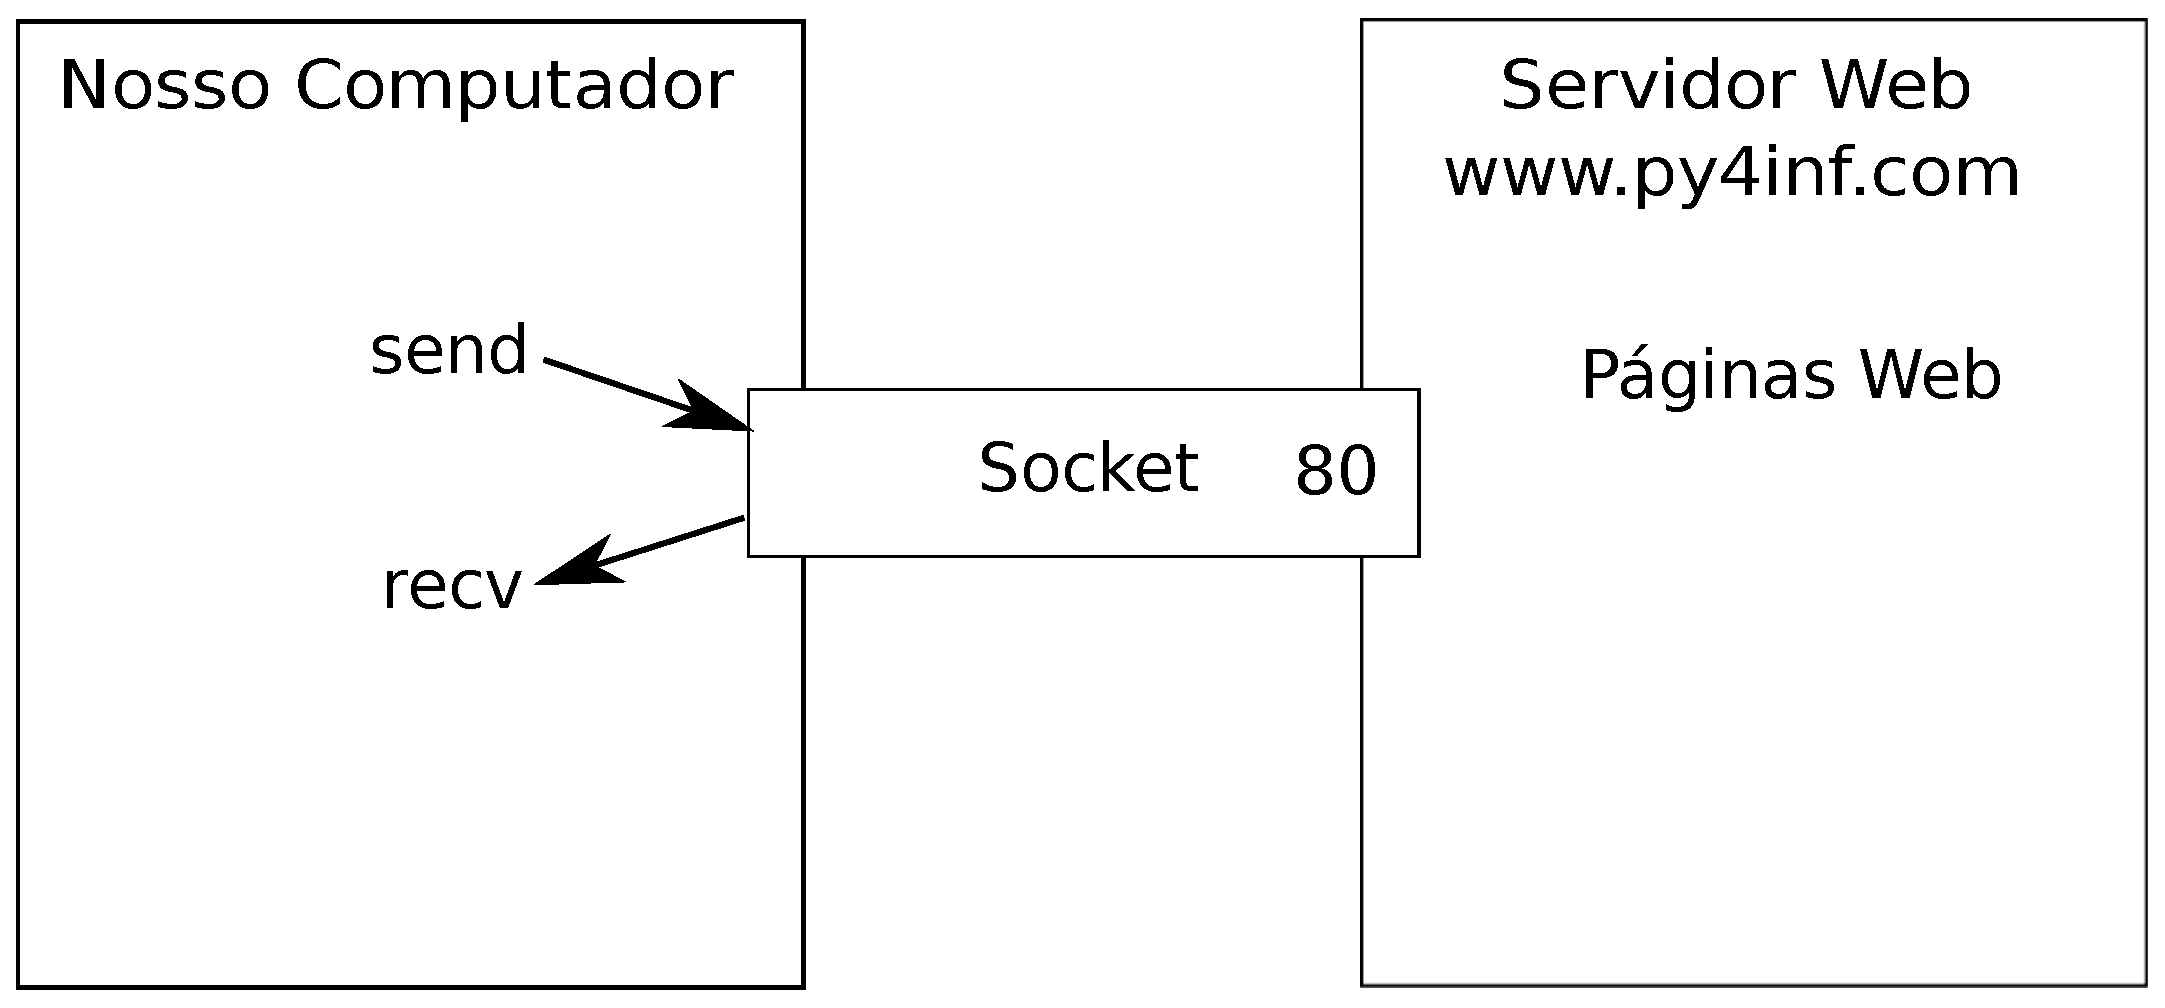
\includegraphics[height=1.50in]{figs2/socket.eps}}
\afterfig

Uma vez enviada a linha em branco, escrevemos um loop que recebe do
socket, dados em pedaços de 512 caracteres e imprime os dados até que não
exista mais dados para ler (por exemplo, a recv() retorna uma string vazia).
%Once we send that blank line, we write a loop that receives data 
%in 512-character chunks from the socket and prints the data out 
%until there is no more data to read (i.e., the recv() returns 
%an empty string).

O programa produz a seguinte saída:
%The program produces the following output:

\beforeverb
\begin{verbatim}
HTTP/1.1 200 OK
Date: Sun, 14 Mar 2010 23:52:41 GMT
Server: Apache
Last-Modified: Tue, 29 Dec 2009 01:31:22 GMT
ETag: "143c1b33-a7-4b395bea"
Accept-Ranges: bytes
Content-Length: 167
Connection: close
Content-Type: text/plain

But soft what light through yonder window breaks
It is the east and Juliet is the sun
Arise fair sun and kill the envious moon
Who is already sick and pale with grief
\end{verbatim}
\afterverb

A saída começa com os cabeçalhos que o servidor web envia para descrever o
documento. Por exemplo, o cabeçalho {\tt Content-Type} indica que o documento
é um documento em texto plano ({\tt text/plain}).
%The output starts with headers which the web server sends
%to describe the document.
%For example, the {\tt Content-Type} header indicates that
%the document is a plain text document ({\tt text/plain}).

Depois que o servidor nos enviar os cabeçalhos, ele adiciona uma linha em branco
para indicar o final dos cabeçalhos, e então, envia realmente os dados do
arquivo {\tt romeo.txt}.
%After the server sends us the headers, it adds a blank line
%to indicate the end of the headers, and then sends the actual
%data of the file {\tt romeo.txt}.

Esse exemplo mostra como fazer uma conexão de rede de baixo nível com sockets.
Sockets podem ser usados para se comunicar com um servidor web ou com um
servidor de e-mail ou muitos outros tipos de servidores. Tudo que é preciso é
encontrar o documento que descreve o protocolo e escrever o código para enviar
e receber os dados de acordo com o protocolo.
%This example shows how to make a low-level network connection
%with sockets.   Sockets can be used to communicate with a web
%server or with a mail server or many other kinds of servers.
%All that is needed is to find the document which describes
%the protocol and write the code to send and receive the data
%according to the protocol.

Contudo, como o protocolo que nós usamos mais  comumente é o protocolo web
HTTP, o Python tem uma biblioteca especificamente desenvolvida para ter suporte
ao protocolo HTTP. E assim, obter documentos e dados através da web.
%However, since the protocol that we use most commonly is
%the HTTP web protocol, Python has a special 
%library specifically designed to support the HTTP protocol 
%for the retrieval of documents and data over the web.

\section{Obtendo uma imagem através do HTTP}
%\section{Retrieving an image over HTTP}

\index{urllib!image}
\index{image!jpg}
\index{jpg}
No exemplo acima, nós pegamos um arquivo em texto plano que tinha novas linhas
dentro do arquivo e nós simplesmente copiamos os dados para a tela a medida
que o programa era executado. Nós podemos usar um programa similar para obter
uma imagem através da web usando o HTTP. Ao invés de copiar os dados para a
tela, a medida que o programa é executado, nós acumulamos os dados em uma
string, retiramos os cabeçalhos, e então salvamos os dados da imagem em um
arquivo. Como a seguir:
%In the above example, we retrieved a plain text file 
%which had newlines in the file and we simply copied the
%data to the screen as the program ran.   We can use a similar
%program to retrieve an image across using HTTP.   Instead
%of copying the data to the screen as the program runs,
%we accumulate the data in a string, trim off the headers,
%and then save the image data to a file as follows:

\beforeverb
\begin{verbatim}
import socket
import time

mysock = socket.socket(socket.AF_INET, socket.SOCK_STREAM)
mysock.connect(('www.py4inf.com', 80))
mysock.send('GET http://www.py4inf.com/cover.jpg HTTP/1.0\n\n')


count = 0
picture = "";
while True:
    data = mysock.recv(5120)
    if ( len(data) < 1 ) : break
    # time.sleep(0.25)
    count = count + len(data)
    print len(data),count
    picture = picture + data

mysock.close()

# Look for the end of the header (2 CRLF)
pos = picture.find("\r\n\r\n");
print 'Header length',pos
print picture[:pos]

# Skip past the header and save the picture data
picture = picture[pos+4:]
fhand = open("stuff.jpg","wb")
fhand.write(picture);
fhand.close()
\end{verbatim}
\afterverb

Quando o programa é executado, ele produz a seguinte saída:
%When the program runs it produces the following output:

\beforeverb
\begin{verbatim}
$ python urljpeg.py 
2920 2920
1460 4380
1460 5840
1460 7300
...
1460 62780
1460 64240
2920 67160
1460 68620
1681 70301
Header length 240
HTTP/1.1 200 OK
Date: Sat, 02 Nov 2013 02:15:07 GMT
Server: Apache
Last-Modified: Sat, 02 Nov 2013 02:01:26 GMT
ETag: "19c141-111a9-4ea280f8354b8"
Accept-Ranges: bytes
Content-Length: 70057
Connection: close
Content-Type: image/jpeg
\end{verbatim}
\afterverb

Você pode ver que para esta url, o cabeçalho {\tt Content-Type} indica que o
corpo do documento é uma imagem ({\tt image/jpeg}). Uma vez terminado o
programa, você pode ver os dados da imagem abrindo o arquivo {\tt stuff.jpg}
com um visualizador de imagens.
%You can see that for this url, the 
%{\tt Content-Type} header indicates that
%body of the document is an image ({\tt image/jpeg}).
%Once the program completes, you can view the image data by opening
%the file {\tt stuff.jpg} in an image viewer.

Durante a execução do programa, você pode ver que não temos 5120 caracteres
para cada vez que chamamos o método {\tt recv()}. Nós pegamos tantos
caracteres quantos foram transferidos através da rede, do servidor web para
nós, no momento que chamamos {\tt recv()}.  Neste exemplo, pegamos 1460 ou 2920
caracteres a cada vez que requisitamos até chegar a 5120 caracteres de dados.
%As the program runs, you can see that we don't get 5120 characters
%each time we call the {\tt recv()} method.
%We get as many characters as have been transferred across the network 
%to us by the web server at the moment we call {\tt recv()}.  
%In this example, we either get 1460 or 2920 characters each time we
%request up to 5120 characters of data.

Os seus resultados podem ser diferentes, dependendo da velocidade de
sua rede.  Note também que na última chamada de {\tt recv()}, nós pegamos
1681 bytes, que é o final do fluxo (stream), e na chamada seguinte da
{\tt recv()} nós recebemos uma string vazia (zero-length). Que nos informa
que o servidor chamou {\tt close()} no seu final de socket e não existe mais
dados para enviar.
%Your results may be different depending on your network speed.  Also
%note that on the last call to {\tt recv()} we get 1681 bytes, which is the end
%of the stream, and in the next call to {\tt recv()} we get a zero-length
%string that tells us that the server has called {\tt close()} on its end 
%of the socket and there is no more data forthcoming.

\index{time}
\index{time.sleep}
Nós podemos reduzir nossas sucessivas chamadas a {\tt recv()} descomentando
, removendo o caractere cerquilha, da chamada de {\tt time.sleep()}.  
Desta forma, nós esperamos
um quarto de segundo depois de cada chamada, e assim, o servidor pode
``se antecipar'' à nós e enviar mais dados antes de nós chamarmos
{\tt recv()} novamente.  Com esse "atraso", o programa é executado
como a seguir:
\beforeverb
\begin{verbatim}
$ python urljpeg.py 
1460 1460
5120 6580
5120 11700
...
5120 62900
5120 68020
2281 70301
Header length 240
HTTP/1.1 200 OK
Date: Sat, 02 Nov 2013 02:22:04 GMT
Server: Apache
Last-Modified: Sat, 02 Nov 2013 02:01:26 GMT
ETag: "19c141-111a9-4ea280f8354b8"
Accept-Ranges: bytes
Content-Length: 70057
Connection: close
Content-Type: image/jpeg
\end{verbatim}
\afterverb

Agora, ao invés de uma primeira e última chamada a {\tt recv()}, nós agora
pegamos 5120 caracteres a cada vez que pedimos novos dados.  
%Now other than the first and last calls to {\tt recv()}, we now get 
%5120 characters each time we ask for new data.  

Existe um buffer entre o servidor, fazendo solicitações {\tt send()} 
e nossa aplicação fazendo solicitações {\tt recv()}.  Quando nós
executamos o programa com o "atraso" estando ativo, em algum momento
o servidor preenche o buffer no socket e é forçado a fazer uma pausa
até que nosso programa comece a esvaziar o buffer.  A pausa, tanto do
envio quanto do recebimento da aplicação, é chamada ``flow control''
(controle de fluxo).
\index{flow control}
%There is a buffer between the server making {\tt send()} requests 
%and our application making {\tt recv()} requests.  When we run the 
%program with the delay in place, at some point the server might 
%fill up the buffer in the socket and be forced to pause until our
%program starts to empty the buffer.  The pausing of either the 
%sending application or the receiving application is called 
%``flow control''.
%\index{flow control}

\section{Obtendo páginas web com {\tt urllib}}
%\section{Retrieving web pages with {\tt urllib}}

Embora nós possamos manualmente enviar e receber dados pelo HTTP 
usando a biblioteca socket, existe uma maneira muito mais simples
de realizar essa tarefa comum em Python pelo uso da biblioteca
{\tt urllib}.
%While we can manually send and receive data over HTTP 
%using the socket library, there is a much simpler way to 
%perform this common task in Python by 
%using the {\tt urllib} library.

Usando a {\tt urllib}, você pode tratar uma página web
de maneira muito parecida a um arquivo. Você simplesmente
indica qual página web você gostaria de obter e a
{\tt urllib} lida com todo o protocolo HTTP e detalhes sobre
cabeçalhos.
%Using {\tt urllib},
%you can treat a web page much like a file.   You simply
%indicate which web page you would like to retrieve and
%{\tt urllib} handles all of the HTTP protocol and header 
%details.

O código equivalente para ler o arquivo {\tt romeo.txt} a partir
da web usando a {\tt urllib} é como o seguinte:
%The equivalent code to read the {\tt romeo.txt} file
%from the web using {\tt urllib} is as follows:

\beforeverb
\begin{verbatim}
import urllib

fhand = urllib.urlopen('http://www.py4inf.com/code/romeo.txt')
for line in fhand:
   print line.strip()
\end{verbatim}
\afterverb

Uma vez que a página web tenha sido aberta com 
{\tt urllib.urlopen}, nós podemos tratá-la
como um arquivo e fazer a leitura usando um loop
{\tt for}.   
%Once the web page has been opened with 
%{\tt urllib.urlopen}, we can treat it like 
%a file and read through it using a 
%{\tt for} loop.   

Quando o programa é executado, nós apenas vemos na
saída o conteúdo do arquivo. Os cabeçalhos
continuam sendo enviados, mas o código da {\tt urllib}
consome os cabeçalhos e apenas retorna os dados para
nós.
%When the program runs, we only see the output
%of the contents of the file.   The headers
%are still sent, but the {\tt urllib} code
%consumes the headers and only returns the 
%data to us.

\beforeverb
\begin{verbatim}
But soft what light through yonder window breaks
It is the east and Juliet is the sun
Arise fair sun and kill the envious moon
Who is already sick and pale with grief
\end{verbatim}
\afterverb

Como um exemplo, nós podemos escrever 
um programa para obter os dados de
{\tt romeo.txt} e calcular a frequência
de cada palavra existente dentro do arquivo como a seguir:
%As an example, we can write 
%a program to retrieve the data for
%{\tt romeo.txt} and compute the frequency
%of each word in the file as follows:

\beforeverb
\begin{verbatim}
import urllib

counts = dict()
fhand = urllib.urlopen('http://www.py4inf.com/code/romeo.txt')
for line in fhand:
    words = line.split()
    for word in words:
        counts[word] = counts.get(word,0) + 1   
print counts
\end{verbatim}
\afterverb

Novamente, uma vez que nós abrimos a página web, 
podemos fazer a leitura como um arquivo local.
%Again, once we have opened the web page, 
%we can read it like a local file.

\section{Analizando o HTML e varrendo a web}
\index{web!scraping}
\index{parsing HTML}
%\section{Parsing HTML and scraping the web}
%\index{web!scraping}
%\index{parsing HTML}

Um dos usos comuns da capacidade da {\tt urllib} em Python é 
{\bf varrer} a web. Varrer a web é quando nós escrevemos um programa
que finge ser um navegador web e obtêm páginas, e então examina os dados
nessas páginas a procura de padrões.
%One of the common uses of the {\tt urllib} capability in Python is 
%to {\bf scrape} the web.   Web scraping is when we write a program
%that pretends to be a web browser and retrieves pages, then 
%examines the data in those pages looking for patterns.

Como um exemplo, um mecanismo de busca como o Google irá olhar os fontes
de uma página web e extrair os links para outras páginas e obter
essas páginas, extrair os links para outras páginas e obter essas
páginas, extrair links e assim por diante. Usando essa técnica,
o Google {\bf mapeia} seu caminho através de quase todas as páginas
na web.   
%As an example, a search engine such as Google will look at the source 
%of one web page and extract the links to other pages and retrieve
%those pages, extracting links, and so on.   Using this technique,
%Google {\bf spiders} its way through nearly all of the pages on 
%the web.   

O Google também usa a frequência de links das páginas que ele encontra
para uma página em particular de maneira a medir o quão ``importante'' 
uma página é, e em que altura a página deve aparecer em seus resultados de
pesquisa.
%Google also uses the frequency of links from pages it finds 
%to a particular page as one measure of how ``important'' 
%a page is and how high the page should appear in its search results.

\section{Analisando o HTML através do uso de expressões regulares}
%\section{Parsing HTML using regular expressions}

Uma maneira simples de analisar o HTML é usar expressões regulares, para
repetidamente, buscar por e extrair substrings que coincidam com um
padrão em particular.
%One simple way to parse HTML is to use regular expressions to repeatedly
%search for and extract substrings that match a particular pattern.

Aqui está uma página web simples:
%Here is a simple web page:

\beforeverb
\begin{verbatim}
<h1>The First Page</h1>
<p>
If you like, you can switch to the
<a href="http://www.dr-chuck.com/page2.htm">
Second Page</a>.
</p>
\end{verbatim}
\afterverb

Nós podemos construir uma expressão regular bem formada para
identificar e extrair os valores dos links do texto abaixo,
como a seguir:
%We can construct a well-formed regular expression to match
%and extract the link values from the above text as follows:

\beforeverb
\begin{verbatim}
href="http://.+?"
\end{verbatim}
\afterverb

Nossa expressão regular procura por strings que iniciam com
``href="http://'', seguida de um ou mais caracteres
(``.+?''), seguida por outra aspas.  O ponto de interrogação 
adicionado ao ``.+?'' indica que a expressão é para coincidir
com um padrão de forma ``não gananciosa'', ao invés de uma
maneira ``gananciosa''. Um padrão não ganancioso tenta encontrar
a {\em menor} string correspondente possível e a gananciosa tenta
encontrar a {\em maior} string correspondente possível.
\index{greedy}
\index{non-greedy}
%Our regular expression looks for strings that start with
%``href="http://'', followed by one or more characters
%(``.+?''), followed by another double quote.  The question mark 
%added to the ``.+?'' indicates that the match is to be done
%in a ``non-greedy'' fashion instead of a ``greedy'' fashion.  
%A non-greedy match tries to find the {\em smallest} possible matching
%string and a greedy match tries to find the {\em largest} possible
%matching string.
%\index{greedy}
%\index{non-greedy}

Nós adicionamos parênteses a nossa expressão regular para indicar
qual parte de nossa string correspondente nós gostaríamos de extrair, e
foi produzido o seguinte programa:
\index{regex!parentheses}
\index{parentheses!regular expression}
%We add parentheses to our regular expression to indicate
%which part of our matched string we would like to extract, and
%produce the following program:
%\index{regex!parentheses}
%\index{parentheses!regular expression}

\beforeverb
\begin{verbatim}
import urllib
import re

url = raw_input('Enter - ')
html = urllib.urlopen(url).read()
links = re.findall('href="(http://.*?)"', html)
for link in links:
    print link
\end{verbatim}
\afterverb

O método de expressão regular {\tt findall} irá retornar para nós uma
lista de todas as strings que coincidem com nossa expressão regular,
retornando apenas o texto do link entre as aspas duplas.
%The {\tt findall} regular expression method will give us a list of all
%of the strings that match our regular expression, returning only
%the link text between the double quotes.

Quando nós executamos o programa, nós temos a seguinte saída:
%When we run the program, we get the following output:

\beforeverb
\begin{verbatim}
python urlregex.py 
Enter - http://www.dr-chuck.com/page1.htm
http://www.dr-chuck.com/page2.htm

python urlregex.py 
Enter - http://www.py4inf.com/book.htm
http://www.greenteapress.com/thinkpython/thinkpython.html
http://allendowney.com/
http://www.py4inf.com/code
http://www.lib.umich.edu/espresso-book-machine
http://www.py4inf.com/py4inf-slides.zip
\end{verbatim}
\afterverb

As expressões regulares funcionam muito bem quando o seu HTML está bem
formatado e previsível.  Mas como existem muitas páginas HTML ``quebradas''
por aí, a solução usando expressões regulares pode tanto perder alguns
links válidos quanto terminar com dados ruins.
%Regular expressions work very nicely when your HTML is well formatted
%and predictable.  But since there are a lot of ``broken'' HTML pages
%out there, a solution only using regular expressions might either miss
%some valid links or end up with bad data.

Isso pode ser resolvido pelo uso de uma robusta biblioteca de análise
de HTML.
%This can be solved by using a robust HTML parsing library.

\section{Analisando o HTML com o uso da BeautifulSoup}
\index{BeautifulSoup}
%\section{Parsing HTML using BeautifulSoup}
%\index{BeautifulSoup}

Existem várias bibliotecas Python que podem ajudar você a analisar
o HTML e extrair dados das páginas.  Cada uma das bibliotecas
tem suas vantagens e desvantagens e você pode escolher uma com base
em suas necessidades.
%There are a number of Python libraries which can help you parse
%HTML and extract data from the pages.  Each of the libraries
%has its strengths and weaknesses and you can pick one based on 
%your needs.

Como exemplo, iremos simplesmente analisar alguma entrada HTML 
e extrair os links usando a biblioteca {\bf BeautifulSoup}.   
Você pode baixar e instalar o código BeautifulSoup de:
%As an example, we will simply parse some HTML input 
%and extract links using the {\bf BeautifulSoup} library.   
%You can download and install the BeautifulSoup code
%from:

\url{http://www.crummy.com/software/}
%\url{http://www.crummy.com/software/}

Você pode baixar e fazer o ``install'' de BeautifulSoup ou 
pode simplesmente colocar o arquivo {\tt BeautifulSoup.py} no mesmo
diretório que está a sua aplicação.
%You can download and ``install'' BeautifulSoup or you 
%can simply place the {\tt BeautifulSoup.py} file in the
%same folder as your application.

Ainda que o HTML se pareça com XML\footnote{O formato XML format será
descrito no próximo capítulo.} e algumas páginas são cuidadosamente 
construídas para ser um XML, a maioria do HTML é, geralmente, quebrado.
O que faz com que um analisador XML rejeite toda a página HTML por
concluir que ela está impropriamente formada. A BeautifulSoup tolera
muitas imperfeições HTML e ainda consegue que você extraia facilmente
os dados que você precisa.
%Even though HTML looks like XML\footnote{The XML format is described in
%the next chapter.} and some pages are carefully 
%constructed to be XML, most HTML is generally broken in ways
%that cause an XML parser to reject the entire page of HTML as
%improperly formed.  BeautifulSoup tolerates highly flawed 
%HTML and still lets you easily extract the data you need.

Nós iremos usar a {\tt urllib} para ler a página e então usar a
{\tt BeautifulSoup} para extrair os atributos {\tt href} das tags
de ancoragem ({\tt a}).
\index{BeautifulSoup}
\index{HTML}
\index{parsing!HTML}
%We will use {\tt urllib} to read the page and then use
%{\tt BeautifulSoup} to extract the {\tt href} attributes from the
%anchor ({\tt a}) tags.
%\index{BeautifulSoup}
%\index{HTML}
%\index{parsing!HTML}

\beforeverb
\begin{verbatim}
import urllib
from BeautifulSoup import *

url = raw_input('Enter - ')
html = urllib.urlopen(url).read()
soup = BeautifulSoup(html)

# Retrieve all of the anchor tags
tags = soup('a')
for tag in tags:
   print tag.get('href', None)
\end{verbatim}
\afterverb

O programa pede um endereço web, e então abre a página web,
lê os dados e passa os dados para o analisador BeautifulSoup, 
e então obtém todas as tags de ancoragem e imprime o atributo
{\tt href} de cada tag.
%The program prompts for a web address, then opens the web
%page, reads the data and passes the data to the BeautifulSoup
%parser, and then retrieves all of the anchor tags and prints
%out the {\tt href} attribute for each tag.

Quando o programa é executado, ele se parece como a seguir:
%When the program runs it looks as follows:

\beforeverb
\begin{verbatim}
python urllinks.py 
Enter - http://www.dr-chuck.com/page1.htm
http://www.dr-chuck.com/page2.htm

python urllinks.py 
Enter - http://www.py4inf.com/book.htm
http://www.greenteapress.com/thinkpython/thinkpython.html
http://allendowney.com/
http://www.si502.com/
http://www.lib.umich.edu/espresso-book-machine
http://www.py4inf.com/code
http://www.pythonlearn.com/
\end{verbatim}
\afterverb

Você pode usar a BeautifulSoup para buscar várias partes de cada 
tag como a seguir:
%You can use BeautifulSoup to pull out various parts of each 
%tag as follows:

\beforeverb
\begin{verbatim}
import urllib
from BeautifulSoup import *

url = raw_input('Enter - ')
html = urllib.urlopen(url).read()
soup = BeautifulSoup(html)

# Retrieve all of the anchor tags
tags = soup('a')
for tag in tags:
   # Look at the parts of a tag
   print 'TAG:',tag
   print 'URL:',tag.get('href', None)
   print 'Content:',tag.contents[0]
   print 'Attrs:',tag.attrs
\end{verbatim}
\afterverb

Isso produz a seguinte saída:
%This produces the following output:

\beforeverb
\begin{verbatim}
python urllink2.py 
Enter - http://www.dr-chuck.com/page1.htm
TAG: <a href="http://www.dr-chuck.com/page2.htm">
Second Page</a>
URL: http://www.dr-chuck.com/page2.htm
Content: [u'\nSecond Page']
Attrs: [(u'href', u'http://www.dr-chuck.com/page2.htm')]
\end{verbatim}
\afterverb

Esses exemplos apenas começam a mostrar o poder da BeautifulSoup,
quando se refere a análise de HTML. Veja a documentação e exemplos
em
\url{http://www.crummy.com/software/BeautifulSoup/} para mais detalhes.
%These examples only begin to show the power of BeautifulSoup
%when it comes to parsing HTML.  See the documentation 
%and samples at
%\url{http://www.crummy.com/software/BeautifulSoup/} for more detail.

\section{Lendo arquivos binários usando a urllib}
%\section{Reading binary files using urllib}

Algumas vezes, você quer obter um arquivo não texto (ou binário), como
um arquivo de imagem ou vídeo. Os dados nesses arquivos geralmente não
são úteis para serem impressos, mas você pode facilmente fazer uma cópia
da URL para um arquivo local em seu disco rígido usando a {\tt urllib}.
\index{binary file}
%Sometimes you want to retrieve a non-text (or binary) file such as
%an image or video file. The data in these files is generally not 
%useful to print out, but you can easily make a copy of a URL to a local
%file on your hard disk using {\tt urllib}.
%\index{binary file}

O padrão é abrir a URL e usar {\tt read} para baixar o conteúdo completo
do documento para dentro de uma variável string ({\tt img}), e então
escrever essa informação em um arquivo local, como a seguir:
%The pattern is to open the URL and use {\tt read} to download the entire
%contents of the document into a string variable ({\tt img}) then write that
%information to a local file as follows:

\beforeverb
\begin{verbatim}
img = urllib.urlopen('http://www.py4inf.com/cover.jpg').read()
fhand = open('cover.jpg', 'w')
fhand.write(img)
fhand.close()
\end{verbatim}
\afterverb

Esse programa lê todos os dados, de uma vez, através da rede e 
os armazena dentro da variável {\tt img}, na principal memória de seu,
computador. Então abre o arquivo {\tt cover.jpg} e escreve os dados para
o seu disco.  Isso irá funcionar se o tamanho do arquivo for menor que
o tamanho da memória de seu computador.
%This program reads all of the data in at once across the network and 
%stores it in the variable {\tt img} in the main memory of your computer,
%then opens the file {\tt cover.jpg} and writes the data out to your 
%disk.  This will work if the size of the file is less than the size
%of the memory of your computer.

Contudo, se ele for um arquivo de áudio ou vídeo grande, esse programa
pode falhar ou pelo menos rodar de forma extremamente vagarosa quando seu
computador ficar sem memória.  Para evitar ficar sem memória, nós podemos
obter os dados em blocos (ou buffers) e então escrever cada bloco no disco
antes de obter o próximo bloco.  Desta forma o programa pode ler um arquivo
de qualquer tamanho sem usar toda a memória que você tem em seu computador.
%However if this is a large audio or video file, this program may crash
%or at least run extremely slowly when your computer runs out of memory.
%In order to avoid running out of memory, we retrieve the data in blocks
%(or buffers) and then write each block to your disk before retrieving
%the next block.  This way the program can read any size file without
%using up all of the memory you have in your computer.

\beforeverb
\begin{verbatim}
import urllib

img = urllib.urlopen('http://www.py4inf.com/cover.jpg')
fhand = open('cover.jpg', 'w')
size = 0
while True:
    info = img.read(100000)
    if len(info) < 1 : break
    size = size + len(info)
    fhand.write(info)

print size,'characters copied.'
fhand.close()
\end{verbatim}
\afterverb

Neste exemplo, nós lemos apenas 100,000 caracteres por vez e então 
escrevemos esses caracteres no arquivo {\tt cover.jpg} antes de obter
os próximos 100,000 caracteres de dados a partir da web.
%In this example, we read only 100,000 characters at a time and then 
%write those characters to the {\tt cover.jpg} file
%before retrieving the next 100,000 characters of data from the
%web.

Esse programa é executado como a seguir:
%This program runs as follows:

\beforeverb
\begin{verbatim}
python curl2.py 
568248 characters copied.
\end{verbatim}
\afterverb

Se você tem um computador Unix ou Macintosh, você provavelmente tem um
comando em seu sistema operacional que executa essa operação,
como a seguir:
\index{curl}
%If you have a Unix or Macintosh computer, you probably have a command
%built in to your operating system that performs this operation
%as follows:
%\index{curl}

\beforeverb
\begin{verbatim}
curl -O http://www.py4inf.com/cover.jpg
\end{verbatim}
\afterverb

O comando {\tt curl} é a abreviação para ``copy URL'', então esses dois 
exemplos são, inteligentemente, chamados de {\tt curl1.py} e {\tt curl2.py} em 
\url{www.py4inf.com/code}, já que eles implementam uma funcionalidade similar
ao comando {\tt curl}.  Existe também um programa exemplo {\tt curl3.py} que
realiza essa tarefa de maneira um pouco mais efetiva, no caso de você
realmente quiser usar esse padrão em um programa que você estiver escrevendo.
%The command {\tt curl} is short for ``copy URL'' and so these two 
%examples are cleverly named {\tt curl1.py} and {\tt curl2.py} on 
%\url{www.py4inf.com/code} as they implement similar functionality
%to the {\tt curl} command.  There is also a {\tt curl3.py} sample 
%program that does this task a little more effectively, in case you
%actually want to use this pattern in a program you are writing.

\section{Glossário}
%\section{Glossary}

\begin{description}
%\begin{description}

\item[BeautifulSoup:] Uma biblioteca Python para análise de documentos HTML
e extração de dados desses documentos HTML que faz compensações nas
maiorias das imperfeições em um HTML que os navegadores geralmente ignoram.
Você pode baixar o código da BeautifulSoup em 
\url{www.crummy.com}.
\index{BeautifulSoup}
%\item[BeautifulSoup:] A Python library for parsing HTML documents
%and extracting data from HTML documents
%that compensates for most of the imperfections in the HTML that browsers
%generally ignore.
%You can download the BeautifulSoup code
%from 
%\url{www.crummy.com}.
%\index{BeautifulSoup}

\item[port:] Um número que geralmente indica qual aplicação 
você está contactando quando você faz uma conexão por socket com um servidor.
Como um exemplo, o tráfego web, usualmente, usa a porta 80, enquanto o
tráfego de e-mail usa a porta 25.
\index{port}
%\item[port:] A number that generally indicates which application 
%you are contacting when you make a socket connection to a server.
%As an example, web traffic usually uses port 80 while email 
%traffic uses port 25.
%\index{port}

\item[scrape:] Quando um programa finge ser um navegador web,
obtém uma página web, e então olha o conteúdo da página web. 
Geralmente os programas estão seguindo os links de uma página para
encontrar a próxima página. Para que eles possam atravessar uma rede de páginas
ou uma rede social.
\index{socket}
%\item[scrape:] When a program pretends to be a web browser and
%retrieves a web page, then looks at the web page content. 
%Often programs are following the links in one page to find the next
%page so they can traverse a network of pages or a social network.
%\index{socket}

\item[socket:] Uma conexão de rede entre duas aplicações. Onde as
aplicações podem enviar e receber dados em ambas as direções.
\index{socket}
%\item[socket:] A network connection between two applications
%where the applications can send and receive data in either direction.
%\index{socket}

\item[spider:] O ato de um mecanismo de busca pela web obtendo uma
página e então todas as páginas com ligações a partir dessa página e
assim por diante até ele ter praticamente todas as páginas na Internet que
ele usará para construir sua indexação de busca.
\index{spider}
%\item[spider:] The act of a web search engine retrieving a page and
%then all the pages linked from a page and so on until they have 
%nearly all of the pages on the Internet which they 
%use to build their search index.
%\index{spider}

\end{description}
%\end{description}

\section{Exercícios}
%\section{Exercises}

\begin{ex}
Altere o programa socket {\tt socket1.py} para pedir ao usuário a 
URL, e assim, ele possa ler qualquer página web.  
Você pode usar {\tt split('/')} para quebrar a URL em partes de componentes
para que você possa extrair o nome da máquina para a chamada {\tt connect}.
Adicionar uma checagem de erro usando {\tt try} e {\tt except} para lidar
com a conexão, caso o usuário digite um formato de URL impróprio ou
não existente.  
\end{ex}
%\begin{ex}
%Change the socket program {\tt socket1.py} to prompt the user for 
%the URL so it can read any web page.  
%You can use {\tt split('/')} to break the URL into its component parts
%so you can extract the host name for the socket {\tt connect} call.
%Add error checking using {\tt try} and {\tt except} to handle the condition where the 
%user enters an improperly formatted or non-existent URL.  
%\end{ex}

\begin{ex}
Altere seu programa socket para que ele conte o número de caracteres que ele
tenha recebido e interrompa a exibição de qualquer texto após ele ter mostrado
3000 caracteres.  O programa deve obter o documento por inteiro, contar o
número total de caracteres e exibir a contagem do número de caracteres no
final do documento.
\end{ex}
%\begin{ex}
%Change your socket program so that it counts the number of characters it has received 
%and stops displaying any text after it has shown 3000 characters.  The program 
%should retrieve the entire document and count the total number of characters 
%and display the count of the number of characters at the end of the document.
%\end{ex}

\begin{ex}
Use a {\tt urllib} para replicar o exercício prévio de (1) obtenção de um
documento a partir de uma URL, (2) exibindo até 3000 caracteres, e (3) 
desfazendo a contagem do total de caracteres no documento.  Não se preocupe
com os cabeçalhos neste exercício, apenas mostre os primeiros 3000 caracteres
do conteúdo do documento.
\end{ex}
%\begin{ex}
%Use {\tt urllib} to replicate the previous exercise of (1) retrieving the document
%from a URL, (2) displaying up to 3000 characters, and (3) counting the overall number
%of characters in the document.  Don't worry about the headers for this exercise, simply
%show the first 3000 characters of the document contents.
%\end{ex}

\begin{ex}
Altere o programa {\tt urllinks.py} para que ele extraia e conte 
as tags parágrafo (p) de um documento HTML obtido e exiba a contagem
de parágrafos como saída de seu programa.  
Não exiba o texto de parágrafo, apenas faça a contagem.
Teste seu programa em várias páginas web pequenas. E também em algumas
páginas web grandes.
\end{ex}
%\begin{ex}
%Change the {\tt urllinks.py} program to extract and count 
%paragraph (p) tags from the retrieved HTML document and 
%display the count of the paragraphs as the 
%output of your program.  
%Do not display the paragraph text, only count them.
%Test your program on several small web pages
%as well as some larger web pages.
%\end{ex}

\begin{ex}
(Avançado) Altere o programa socket para que ele apenas mostre os dados
após os cabeçalhos e uma linha em branco tiverem sido recebidos. Lembre 
que o {\tt recv} está recebendo caracteres (nova linha e outros mais),
não linhas.
\end{ex}
%\begin{ex}
%(Advanced) Change the socket program so that it only shows data after the 
%headers and a blank line have been received.  Remember that {\tt recv} is
%receiving characters (newlines and all), not lines.
%\end{ex}

% TODO % The contents of this file is 
% Copyright (c) 2009-  Charles R. Severance, All Righs Reserved

\chapter{Usando Web Services}
%\chapter{Using Web Services}

Agora que se tornou mais facil retornar e analizar documentos
HTTP utilizando programas, não levará muito tempo para desenvolver
um sistema onde nós podemos começar à produzir documentos que serão
especificamente projetados para serem utilizados por outros
programas (i.e., não é o HTML que é mostrado no navegador).
%Once it became easy to retrieve documents and parse documents 
%over HTTP using programs, it did not take long to develop 
%an approach where we started producing documents that were specifically
%designed to be consumed by other 
%programs (i.e., not HTML to be displayed in a browser).

Existem dois formatos comuns que nós usamos quando trocamos dados através da web.
O ``eXtensible Markup Language'' ou XML é utilizado à muito tempo
e é melhor projetado para troca de document-style-data. Quando programas somente
querem trocar dicionarios, listas, ou outra informaçao interterna entre eles, 
eles usam JavaScript Object Notation ou JSON (sobre \url{www.json.org}).
Nós vamos ver os dois formatos.
%There are two common formats that we use when exchanging data across the web.
%The ``eXtensible Markup Language'' or XML has been in use for a very long time 
%and is best suited for exchanging document-style data.   When programs just want 
%to exchange dictionaries, lists, or other internal information with each other,
%they use JavaScript Object Notation or JSON (see \url{www.json.org}).  
%We will look at both formats.

\section{eXtensible Markup Language - XML}
%\section{eXtensible Markup Language - XML}

O XML é bem parecido com o HTML, porem o XML é melhor estruturado
que o HTML. Aqui está um exemplo de um documento XML:
%XML looks very similar to HTML, but XML is more structured 
%than HTML.  Here is a sample of an XML document:

\beforeverb
\begin{verbatim}
<person>
  <name>Chuck</name>
  <phone type="intl">
     +1 734 303 4456
   </phone>
   <email hide="yes"/>
</person>
\end{verbatim}
\afterverb
%
É mais facil pensar em um documento XML como uma estrutura em arvore
onde tem uma tag no topo {\tt person} e outras tags como {\tt phone}
são escritas como \emph{filhos} dos pais deles. 
%Often it is helpful to think of an XML document as a tree structure
%where there is a top tag {\tt person} and other tags such as {\tt phone}
%are drawn as \emph{children} of their parent nodes.

\beforefig
\centerline{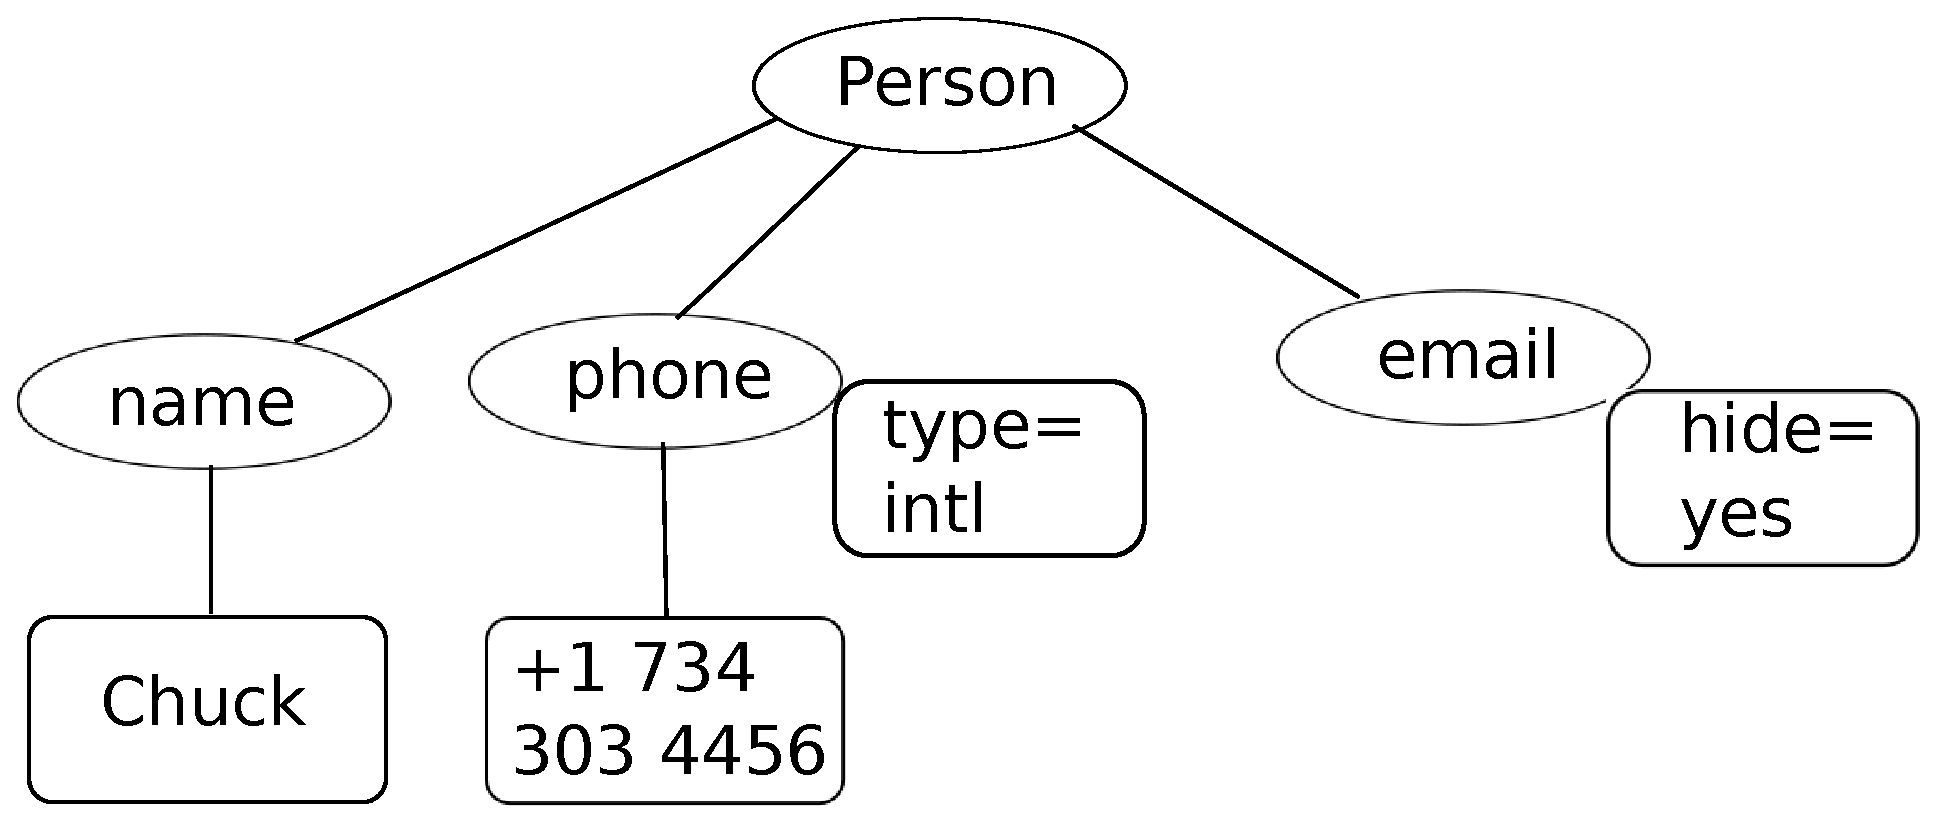
\includegraphics[height=1.50in]{figs2/xml-tree.eps}}
\afterfig

\section{Analizando o XML}
%\section{Parsing XML}

\index{ElementTree}
\index{ElementTree!fromstring}
\index{ElementTree!find}

Aqui está uma simples aplicação que analiza algum XML
e extrai alguns elementos do XML:
%Here is a simple application that parses some XML
%and extracts some data elements from the XML:

\beforeverb
\begin{verbatim}
import xml.etree.ElementTree as ET

data = '''
<person>
  <name>Chuck</name>
  <phone type="intl">
     +1 734 303 4456
   </phone>
   <email hide="yes"/>
</person>'''

tree = ET.fromstring(data)
print 'Name:',tree.find('name').text
print 'Attr:',tree.find('email').get('hide')
\end{verbatim}
\afterverb
%
Ao chamar {\tt fromstring} é feita a conversão da string que 
representa o XML em uma ``arvore'' de conecções XML. Quando o
XML esta em uma arvore, nós temos uma serie de metodos que nós
podemos chamar para exrair informações do XML.
%Calling {\tt fromstring} converts the string representation
%of the XML into a ``tree'' of XML nodes.  When the
%XML is in a tree, we have a series of methods we can call to 
%extract portions of data from the XML.  

A função {\tt find} varre a arvore do XML
e retorna um {\bf nó} que corresponde à aquela tag especifica.
Cada nó pode conter algum texto, alguns atributos (como hide), e
algum nó ``filho''. Cada nó pode ser o inicio de uma arvore de nós.
%The {\tt find} function searches through the 
%XML tree and retrieves a {\bf node} that matches the specified tag.
%Each node can have some text, some attributes (like hide), and
%some ``child'' nodes.   Each node can be the top of a tree of nodes.

\beforeverb
\begin{verbatim}
Name: Chuck
Attr: yes
\end{verbatim}
\afterverb
%
Utilizar um analizador de XML como o {\tt ElementTree} teremos a
vantagem que, enquanto o XML deste exemplo é bastante simples, 
teremos muitas regras em relação à XML validos e usar o 
{\tt ElementTree} nos permitirá extrair informações do XML sem
se preoculpar com as regras de sintaxe do XML.
%Using an XML parser such as {\tt ElementTree} has the advantage
%that while the XML in this example is quite simple, it turns
%out there are many rules regarding valid XML and using 
%{\tt ElementTree} allows us to extract data from XML without 
%worrying about the rules of XML syntax.

\section{Percorrendo os nós}
%\section{Looping through nodes}

\index{ElementTree!findall}
\index{ElementTree!get}
Frequentemente o XML terá multiplos nós que nós podemos percorrer
para processar todos os nós. No programa a seguir,
nós percorremos por todos os nós do {\tt user}:
%Often the XML has multiple nodes and we need to write a loop
%to process all of the nodes.  In the following program, 
%we loop through all of the {\tt user} nodes:

\beforeverb
\begin{verbatim}
import xml.etree.ElementTree as ET

input = '''
<stuff>
    <users>
        <user x="2">
            <id>001</id>
            <name>Chuck</name>
        </user>
        <user x="7">
            <id>009</id>
            <name>Brent</name>
        </user>
    </users>
</stuff>'''

stuff = ET.fromstring(input)
lst = stuff.findall('users/user')
print 'User count:', len(lst)

for item in lst:
    print 'Name', item.find('name').text
    print 'Id', item.find('id').text
    print 'Attribute', item.get('x')
\end{verbatim}
\afterverb
%
O metodo {\tt findall} retorna uma lista do Python com sub-árvores
que representam a estrutura {\tt user} da árvore do XML. Então nós 
podemos escrever um loop {\tt for} que procura em cada nó do user,
e imprime os elementos {\tt name} e {\tt id} assim como o 
atributo {\tt x} do nó {\tt user}.
%The {\tt findall} method retrieves a Python list of subtrees that
%represent the {\tt user} structures in the XML tree.  Then we can 
%write a {\tt for} loop that looks at each of the user nodes, and 
%prints the {\tt name} and {\tt id} text elements as well as the 
%{\tt x} attribute from the {\tt user} node.

\beforeverb
\begin{verbatim}
User count: 2
Name Chuck
Id 001
Attribute 2
Name Brent
Id 009
Attribute 7
\end{verbatim}
\afterverb
%

\section{JavaScript Object Notation - JSON}
%\section{JavaScript Object Notation - JSON}
\index{JSON}
\index{JavaScript Object Notation}

O formato JSON foi inspirado no formato do objeto array utilizado na linguagem JavaScript.
Mas como o Python foi inventado antes do JavaScript, a sintaxe que o Python utiliza
para dicionarios e listas influenciaram na sintaxe do JSON. Então o formato JSON é
bem parecido com a combinação de listas e dicionarios do Python.
%The JSON format was inspired by the object and array format used in the JavaScript
%language.  But since Python was invented before JavaScript, Python's syntax
%for dictionaries and lists influenced the syntax of JSON.  So the format of JSON
%is nearly identical to a combination of Python lists and dictionaries.

Aqui está uma codificação JSON que é quase equivalente ao simples XML abaixo:
%Here is a JSON encoding that is roughly equivalent to the simple XML from above:

\beforeverb
\begin{verbatim}
{
  "name" : "Chuck",
  "phone" : {
    "type" : "intl",
    "number" : "+1 734 303 4456"
   },
   "email" : {
     "hide" : "yes"
   }
}
\end{verbatim}
\afterverb
%
Você pode notar algumas diferenças. Primeira, no XML, nós podemos adicionar
atributos como ``intl'' à tag ``phone''. No JSON, nós simplesmente temos chaves de
valores pares. Além de que a tag ``person'' não existe mais, que substituida por
um conjunto de chaves externas.
%You will notice some differences.  First, in XML, we can add attributes like
%``intl'' to the ``phone'' tag.  In JSON, we simply have key-value pairs.  Also
%the XML ``person'' tag is gone, replaced by a set of outer curly braces.  

No geral, a estrutura JSON é mais simples que a do XML por conta do JSON ter menos
utilidades que o XML. Mas o JSON tem a vantagem de mapear {\em directly} para alguma
combinação de dicionarios e listas. E como quase todas as linguagens de programação 
tem algo equivalente aos dicionarios e listas do Python, JSON é um formato natural 
para fazer dois programas cooperarem e trocarem dados.
%In general, JSON structures are simpler than XML because JSON has fewer capabilities
%than XML.  But JSON has the advantage that it maps {\em directly} to some combination
%of dictionaries and lists.   And since nearly all programming languages 
%have something equivalent to Python's dictionaries and lists, JSON is a very
%natural format to have two cooperating programs exchange data.

JSON está facilmente se tornando o formato escolhido para realizar troca de dados
entre aplicações por conta de sua simplicidade se comparado ao XML.
%JSON is quickly becoming the format of choice for nearly all data exchange between 
%applications because of its relative simplicity compared to XML.

\section{Analizando JSON}
%\section{Parsing JSON}

Nós podemos contruir nosso JSON utilizando dicionarios (objetos) e listas conforme
o necessario. Neste exemplo, nós vamos representar uma lista de usuarios onde cada
usuario é um conjunto de pares de valor-chave (i.e., um dicionario). Então nós temos
uma lista de dicionarios.
%We construct our JSON by nesting dictionaries (objects) and lists as needed.  In 
%this example, we represent a list of users where each user is a set of 
%key-value pairs (i.e., a dictionary).  So we have a list of dictionaries.

No programa a seguir, nós usamos o biblioteca contrutora {\bf json} para analizar
o JSON e ler as informações. Compare ele de perto com a informação equivalente em XML
abaixo. O JSON tem menos detalhes, então nós devemos previamente saber que nós
estamos pegando uma lista e essa lista são usuarios e cada usuario é uma valor de 
chave. O JSON é mais sucinto (uma vantagem) mas também é menos auto-explicativo 
(uma desvantagem).
%In the following program, we use the built-in {\bf json} library to parse 
%the JSON and read through the data.   Compare this closely to the equivalent
%XML data and code above.  The JSON has less detail, so we must know in advance 
%that we are getting a list and that the list is of users and each user is a
%set of key-value pairs.  The JSON is more succinct (an advantage) but also is 
%less self-describing (a disadvantage).

\beforeverb
\begin{verbatim}
import json

input = '''
[
  { "id" : "001",
    "x" : "2",
    "name" : "Chuck"
  } ,
  { "id" : "009",
    "x" : "7",
    "name" : "Brent"
  } 
]'''

info = json.loads(input)
print 'User count:', len(info)

for item in info:
    print 'Name', item['name']
    print 'Id', item['id']
    print 'Attribute', item['x']
\end{verbatim}
\afterverb
%

Se você comparar o codigo para extrarir a informação do JSON e XML analizados,
você vera que oque nós pegamos do {\bf json.loads()} é uma lista Python
que nós percorremos com um {\tt for} loop, e cada item dentro desta lista
é um dicionario Python. Uma vez que o JSON foi analizado, nós podemos usar o
operador de indice do Python para extrair varias informações de cada usuario.
Nós não precisamos usar a biblioteca JSON para percorrer o JSON analizado, 
pois ela retornará uma informação já é uma estrutura do proprio Python.
%If you compare the code to extract data from the parsed JSON and XML
%you will see that what we get from {\bf json.loads()} is a Python list
%which we traverse with a {\tt for} loop, and each item within that list
%is a Python dictionary.  Once the JSON has been parsed, we can use the Python
%index operator to extract the various bits of data for each user.  We don't
%have to use the JSON library to dig through the parsed JSON, since the returned
%data is simply native Python structures.

A saida deste programa é exatamente a mesma que a versão em XML abaixo.
%The output of this program is exactly the same as the XML version above.

\beforeverb
\begin{verbatim}
User count: 2
Name Chuck
Id 001
Attribute 2
Name Brent
Id 009
Attribute 7
\end{verbatim}
\afterverb
%
Em geral, existem uma tendencia da industria utilizar cada vez mais o JSON
do que o XML em serviços web. Por conta do JSON ser mais simples e mais
direcionado para estruturas nativas que já existem nas linguagens de
programação, a analize e extração de dados é usualmente simples e mais direto
utilizando JSON. Mas o XML é mais auto-explicativo que o JSON então terá
algumas aplicações em que o XML detem a vantagem. Por exemplo, a maioria de 
processadores de palavras armazenam documentos internamente utilizando XML
em vez de JSON.
%In general, there is an industry trend away from XML and towards JSON for 
%web services.  Because the JSON is simpler and more directly maps to native 
%data structures we already have in programming languages, the parsing 
%and data extraction code is usually simpler and more direct when using JSON.
%But XML is more self-descriptive than JSON and so there are 
%some applications where XML retains an advantage.  For example, most word 
%processors store documents internally using XML rather than JSON.

\section{Interface de Programação de Aplicação}
%\section{Application Programming Interfaces}

Nós agora temos a habilidade de trocar dados entre aplicações utilizando 
HiperText Transport Protocol (HTTP) e uma forma de representar dados complexos
que nós estamos enviando e recebento entre estas aplicações utilizando 
eXtensible Markup Language (XML) ou JavaScript Object Notation (JSON)
%We now have the ability to exchange data between applications using HyperText
%Transport Protocol (HTTP) and a way to represent complex data that we are 
%sending back and forth between these applications using eXtensible 
%Markup Language (XML) or JavaScript Object Notation (JSON).

O proximo passo é começar a definir um documento ``contratos'' entre
aplicações utilizando essas tecnicas. Geralmente o nome para estes contratos
administração-para-administração é {\bf Interface de Programação de 
Aplicação} ou API.Quando nós usamos uma API, geralmente um programa tem 
um conjunto de {\bf serviços} disponiveis para serem usados em outras
aplicações e disponibiliza as APIs (i.e, as ``regras'') que deve ser
seguidas para acessar os serviços disponibilizados pelo programa.
%The next step is to begin to define and document ``contracts'' between 
%applications using these techniques. The general name for these 
%application-to-application contracts is {\bf Application Program 
%Interfaces} or APIs.  When we use an API, generally one program
%makes a set of {\bf services} available for use by other applications
%and publishes the APIs (i.e., the ``rules'') that must be followed to 
%access the services provided by the program.

Quanto nós começamos a construir nossos programas onde a funcionalidade
do nosso programa inclui acessar os servirçoes prestados por outros 
programas, nós chamamos essa abordade de {\bf Arquitetura Orientada
a Serviços} ou SOA. Uma abordagem SOA é no geral onde nossa aplicação
utiliza os serviços de outras aplicações. Uma abordagem não SOA é quando
a aplicação é uma unica aplicação autônoma que contem todo o codigo
necessario para inplementar a aplicação.
%When we begin to build our programs where the functionality of
%our program includes access to services provided by other programs, 
%we call the approach a {\bf Service-Oriented Architecture} or SOA.
%A SOA approach is one where our overall application makes use of 
%the services of other applications.  A non-SOA approach is where the
%application is a single standalone application which contains all of the
%code necessary to implement the application.

Nós vemos varios exemplos de SOA quando utilizamos a internet. Nós podemos
acessar um site e comprar passagens aereas, reservar hoteis, alugar carros
neste unico site. A informaçao dos hoteis não é armazenada nos computadores
das companhias aéreas. Em vez disso, os computadores desta companhia utilizam
os serviços dos computadores dos hoteis e retornam os dados do hotel e
apresentam para o usuario. Quando o usuario concorda em fazer uma reserva de
um hotel usando o site da companhia aérea, o site da companhia utiliza outro 
serviço web que está nos sistemas do hotel onde realmente é realizada a reserva.
E quando chega a hora de utilizar o seu cartão de credito para toda a transação,
outro compudator continual envolvido durante o processo.
%We see many examples of SOA when we use the web.  We can go to a single 
%web site and book air travel, hotels, and automobiles all from a 
%single site.  The data for hotels is not stored on the airline computers. 
%Instead, the airline computers contact the services on the hotel computers
%and retrieve the hotel data and present it to the user.  When the user
%agrees to make a hotel reservation using the airline site, the airline site uses
%another web service on the hotel systems to actually make the reservation.
%And when it comes time to charge your credit card for the whole transaction, 
%still other computers become involved in the process.

\beforefig
\centerline{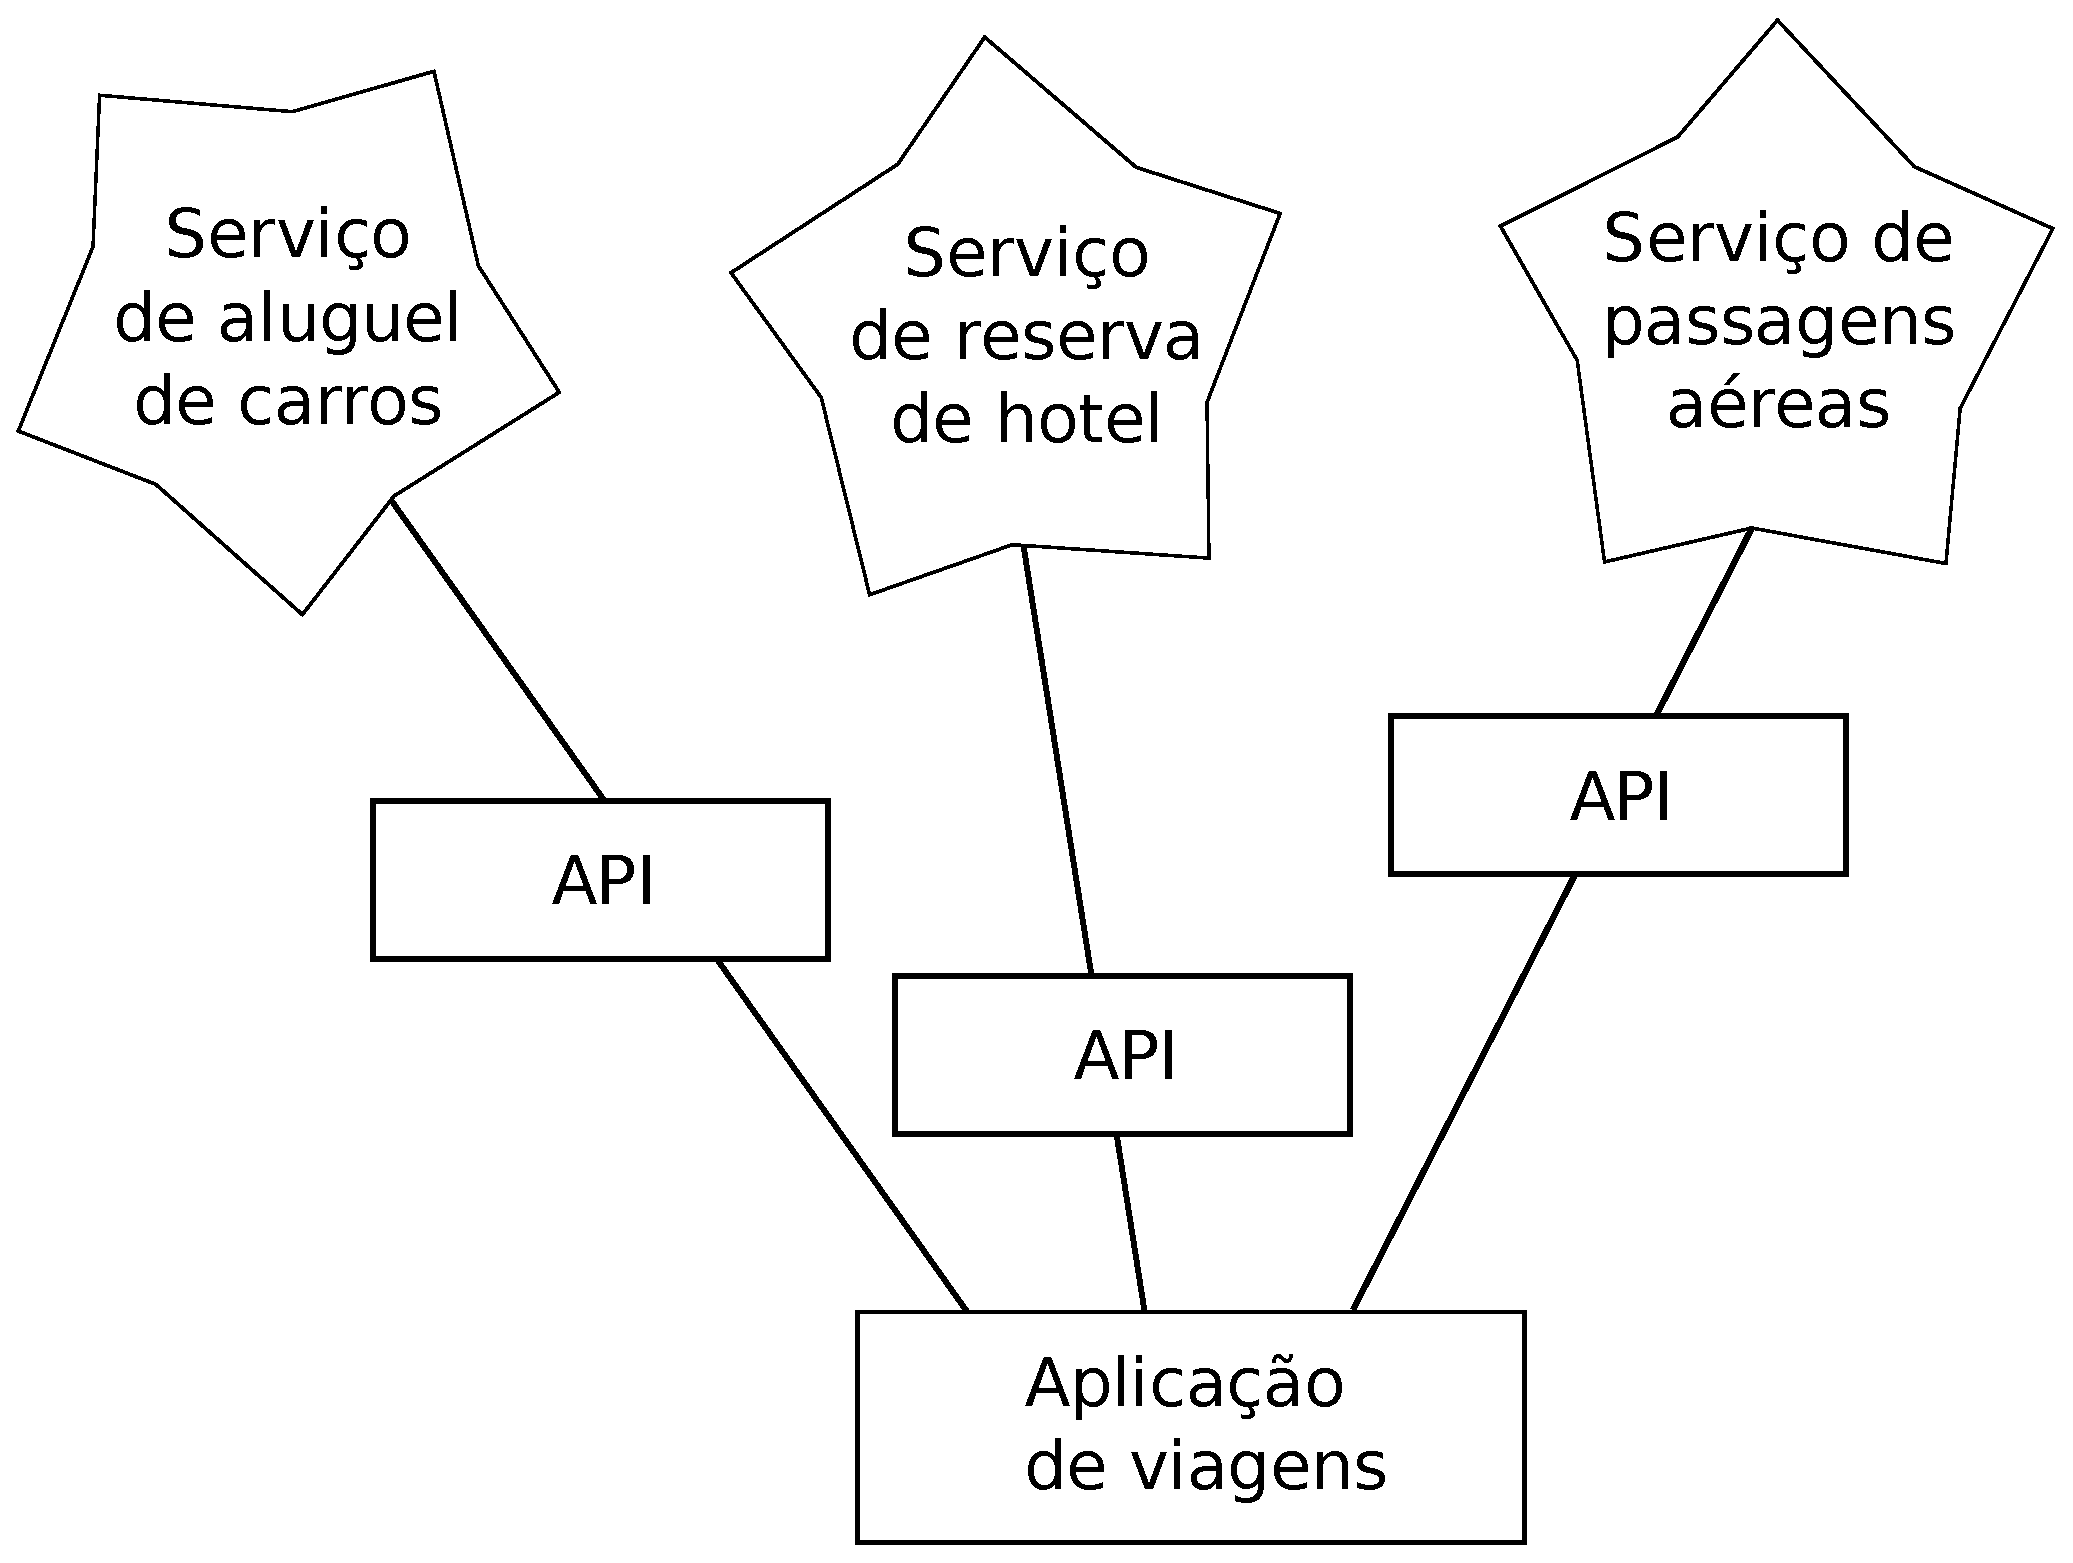
\includegraphics[height=2.50in]{figs2/soa.eps}}
\afterfig
Uma Arquitetura Orientada a Serviços tem muitas vantagens incluindo: (1)
nós sempre manteremos uma copia dos dados (isso é particulamente importante
para coisas como reservas de hoteis onde nós não queremos as duplicar)
e (2) os donos dos dados podem setar regras sobre como usar od dados deles.
Com essas vantagens, um sistema SOA precisa ser cuidadosamente projetado
para ter boa performance e atender as necessidades dos usuarios.
%A Service-Oriented Architecture has many advantages including: (1) we 
%always maintain only one copy of data (this is particularly important
%for things like hotel reservations where we do not want to over-commit)
%and (2) the owners of the data can set the rules about the use of their 
%data.   With these advantages, an SOA system must be carefully designed
%to have good performance and meet the user's needs.

Quando uma aplicação torna os serviçoes em sua API disponiveis para a internet,
nós os chamamos de {\bf serviços web}.
%When an application makes a set of services in its API available over the web, 
%we call these {\bf web services}. 

\section{Serviço web Google de geocodificação}
%\section{Google geocoding web service}
\index{Google}
\index{geocoding}
\index{web service}

O Goole tem um excelente serviço web que nos permite usar seus bancos de
dados de informações geograficas. Nós podemos enviar uma pesquisa geografica 
em forma de string como ``Ann Arbor, MI'' para a API de geodificação deles e o 
Google retornara o seu melhor palpite de em qual lugar do mapa nós podemos 
encontrar o local pesquisado e nos fala sobre lugares nas proximidades. 
%Google has an excellent web service that allows us to make use of their 
%large database of geographic information.   We can submit a geographical
%search string like ``Ann Arbor, MI'' to their geocoding API and have Google 
%return its best guess as to where on a map we might find our search string and
%tell us about the landmarks nearby.


O serviço de geocodificação é gratis, porem limitado, então você não pode fazer
um uso ilimitado da API em serviços comerciais. Mas se você tem alguns dados de
localização que um usuario digitou em uma caixa de entrada, você pode usar
esta API para deixar suas informações mais concisas.
%The geocoding service is free but rate limited so you cannot make unlimited
%use of the API in a commercial application.   But if you have some survey data
%where an end user has entered a location in a free-format input box, you can use
%this API to clean up your data quite nicely.  

{\em Quando você está usando uma API gratis como a de geocodificação do Google,
você precisa ser respeitoso sobre o uso desses recursos. Se muitas pessoas
abusarem do serviço, o Google pode reduzir de forma significante seus serviços
gratuitos.}
%{\em When you are using a free API like Google's geocoding API, you need
%to be respectful in your use of these resources.  If too many people abuse the
%service, Google might drop or significantly curtail its free service.}
\index{rate limiting}

Você pode ler documentos online sobre esse serviço, mas é bem simples e você
pode até testar ele usando um navegador, somente digitando a seguinte URL em
seu navegador:
%You can read the online documentation for this service, but it is quite simple
%and you can even test it using a browser by typing the following URL into your 
%browser:

\url{http://maps.googleapis.com/maps/api/geocode/json?sensor=false &address=Ann+Arbor%2C+MI}

Tenha certeze de resolver a URL e remover qualquer espaço em branco antes de 
colar a URL em seu navegador.
%Make sure to unwrap the URL and remove any spaces from the URL before pasting
%it into your browser.

A seguir temos uma simples aplicação que solicita ao usuario por uma string de
pesquisa, requisita a API de geocodificação do Google, e extrai informações do
JSON que foi retornado.
%The following is a simple application to prompt the user for a search string,
%call the Google geocoding API, and extract information from the returned JSON.

\beforeverb
\begin{verbatim}
import urllib
import json

serviceurl = 'http://maps.googleapis.com/maps/api/geocode/json?'

while True:
    address = raw_input('Enter location: ')
    if len(address) < 1 : break

    url = serviceurl + urllib.urlencode({'sensor':'false', 
          'address': address})
    print 'Retrieving', url
    uh = urllib.urlopen(url)
    data = uh.read()
    print 'Retrieved',len(data),'characters'

    try: js = json.loads(str(data))
    except: js = None
    if 'status' not in js or js['status'] != 'OK':
        print '==== Failure To Retrieve ===='
        print data
        continue

    print json.dumps(js, indent=4)

    lat = js["results"][0]["geometry"]["location"]["lat"]
    lng = js["results"][0]["geometry"]["location"]["lng"]
    print 'lat',lat,'lng',lng
    location = js['results'][0]['formatted_address']
    print location
\end{verbatim}
\afterverb
%
O programa pega a string de pesquisa e constroi uma URL com a string
como um parametro devidamente codificada e então usa o {\bf urllib}
para retornar o texto da API de geodificação do Google. Diferente
de uma pagina web fixa,os dados que pegamos depende dos parametros 
que nós enviamos e as informações geograficas armazenadas nos 
servidores do Google.
%The program takes the search string and constructs a URL with the
%search string as a properly encoded parameter and then uses
%{\bf urllib} to retrieve the text from the Google geocoding API.
%Unlike a fixed web page, the data we get depends on the parameters
%we send and the geographical data stored in Google's servers.

Uma vez que retornamos os dados JSON, nós analizamos isso com a 
biblioteca {\bf json} e fazmos algumas checagens para garantir que 
recebemos a informação correta, então extraimos a informação que 
nós necessitamos.
%Once we retrieve the JSON data, we parse it with the {\bf json}
%library and do a few checks to make sure that we received good data, 
%then extract the information that we are looking for.

A saida do programa está logo a seguir (algum dado retornado no JSON
foi removido):
%The output of the program is as follows (some of the returned
%JSON has been removed):

\beforeverb
\begin{verbatim}
$ python geojson.py
Enter location: Ann Arbor, MI
Retrieving http://maps.googleapis.com/maps/api/
  geocode/json?sensor=false&address=Ann+Arbor%2C+MI
Retrieved 1669 characters
{
    "status": "OK", 
    "results": [
        {
            "geometry": {
                "location_type": "APPROXIMATE", 
                "location": {
                    "lat": 42.2808256, 
                    "lng": -83.7430378
                }
            }, 
            "address_components": [
                {
                    "long_name": "Ann Arbor", 
                    "types": [
                        "locality", 
                        "political"
                    ], 
                    "short_name": "Ann Arbor"
                } 
            ], 
            "formatted_address": "Ann Arbor, MI, USA", 
            "types": [
                "locality", 
                "political"
            ]
        }
    ]
}
lat 42.2808256 lng -83.7430378
Ann Arbor, MI, USA
Enter location:
\end{verbatim}
\afterverb
%
Você pode baixar
\url{www.py4inf.com/code/geojson.py} e
\url{www.py4inf.com/code/geoxml.py} para explorar
variantes de JSON e XML da API de geocodificação do Google.
%You can download 
%\url{www.py4inf.com/code/geojson.py} and 
%\url{www.py4inf.com/code/geoxml.py} to explore the JSON
%and XML variants of the Google geocoding API. 

\section{Segurança e utilizanção de API}
%\section{Security and API usage}
\index{OAuth}
\index{API!key}

É bem comum que você necessite de algum tipo de 
``chave de API'' para fazer uso de uma API de um fornecedor.
A ideia geral é que eles querem saber quem está usando os
seriviços deles e o quanto cada usuario está usando.
Entretanto eles tem partes pagas e gratuitas dos serviçoes
deles, ou tem uma politca que limita o numero de requisições
que um unico individuo pode realizar durante um determinado
periodo de tempo.
%It is quite common that you need some kind of 
%``API key'' to make use of a vendor's API.  The
%general idea is that they want to know who is using 
%their services and how much each user is using.  
%Perhaps they have free and pay tiers of their services
%or have a policy that limits the number of requests 
%that a single individual can make during a particular 
%time period.

Uma vez que você tenha a chave da API, você simplesmente
insere a chave como parte dos dados de POST ou possivelmente
como um parametro da URL que está chamando a API.
%Sometimes once you get your API key, you simply include
%the key as part of POST data or perhaps as a parameter
%on the URL when calling the API.

As vezes, o fornecedor quer aumentar a garantia da 
origem da requisição e então eles esperam que você os
envie mensagens criptografadas usando chaves compartilhadas
e secretas, Uma tecnologia muito comum que é utilizada para 
enviar requisições pela Internet é chamada {\bf OAuth}.
Você pode ler mais sobre o protocolo OAuth em 
\url{http://www.oauth.net}.
%Other times, the vendor wants increased assurance of
%the source of the requests and so they add expect you 
%to send cryptographically signed messages using shared
%keys and secrets.   A very common technology that is used 
%to sign requests over the Internet is called {\bf OAuth}.
%You can read more about the OAuth protocol at
%\url{http://www.oauth.net}.

Como a API do Twitter tornou-se cada vez mais valiosa, o
Twitter virou de uma API aberta e publica para uma API que
requisita o uso da assinatura OAuth em cada requisição a API.
Felizmente ainda existe um numero de bibliotecas OAuth 
convenientes e gratuitas então você pode evitar ter de escrever
uma implementação OAuth do inicio lendo a sobre a especificação.
Estas bibliotecas são de complexidade variante e tem varios
graus de riqueza. O site do OAuth contem informações sobre
diversas bibliotecas OAuth.
%As the Twitter API became increasingly valuable, Twitter
%went from an open and public API to an API that required
%the use of OAuth signatures on each API request. Thankfully
%there are still a number of convenient and free OAuth libraries
%so you can avoid writing an OAuth implementation from scratch
%by reading the specification.  These libraries are of 
%varying complexity and have varying degrees of
%richness.  The OAuth web site has information about various 
%OAuth libraries.

Para este proximo exemplo nós vamos baixar os arquivos
{\bf twurl.py}, {\bf hidden.py}, 
{\bf oauth.py}, 
e
{\bf twitter1.py} a partir do 
\url{www.py4inf.com/code} e colocar todos na mesma pasta
em seu computador.
on your computer.
%For this next sample program we will download the files 
%{\bf twurl.py}, {\bf hidden.py}, 
%{\bf oauth.py}, 
%and
%{\bf twitter1.py} from 
%\url{www.py4inf.com/code} and put them all in a folder
%on your computer.

Para poder usar estes programas você ira precisar ter uma conta
no Twitter, e autorizar seu codigo python como uma aplicação,
configurar uma chave, secreta, chave eletronica e chave eletronica
secreta. Você devera editar o arquivo {\bf hidden.py} e armazenar
estas quatro strings nas variaveis apropriadas no arquivo:
%To make use of these programs you will need to have a Twitter
%account, and authorize your Python code as an application,
%set up a key, secret, token and token secret.  You will edit
%the file {\bf hidden.py} and put these four strings into the
%appropriate variables in the file:

\beforeverb
\begin{verbatim}
    def auth() :
        return { "consumer_key" : "h7L...GNg",
            "consumer_secret" : "dNK...7Q",
            "token_key" : "101...GI",
            "token_secret" : "H0yM...Bo" }
\end{verbatim}
\afterverb
%
O serviço web do Twitter é acessado utilizando uma URL como esta:
%The Twitter web service are accessed using a URL like this:

\url{https://api.twitter.com/1.1/statuses/user_timeline.json}

Uma vez que todas as informações de seguranças tenham sido adicionada,
a URL parecerá com algo assim:
%But once all of the security information has been added, the URL
%will look more like:

\beforeverb
\begin{verbatim}
https://api.twitter.com/1.1/statuses/user_timeline.json?count=2
&oauth_version=1.0&oauth_token=101...SGI&screen_name=drchuck
&oauth_nonce=09239679&oauth_timestamp=1380395644
&oauth_signature=rLK...BoD&oauth_consumer_key=h7Lu...GNg
&oauth_signature_method=HMAC-SHA1
\end{verbatim}
\afterverb
%
Você pode ler a especificação OAuth se você quiser saber mais
sobre o siguinificado dos varios parametros que foram adicionados
para suprir os requerimentos de segurança do OAuth.
%You can read the OAuth specification if you want to
%know more about the meaning of the various parameters that
%are added to meet the security requirements of OAuth.  

Para os programas que utiliza o Twitter, nós escondemos toda
a complexidade nos arquivos {\bf oauth.py} e {\bf twurl.py}.
Nós simplesmente configuramos os segretos em {\bf hidden.py}
e então enviamos a URL desejada paraa função 
{\bf twurl.augment()} e o codigo da biblioteca adiciona todos
os parametros necessarios à URL para nós.
%For the programs we run with Twitter, we hide all the 
%complexity in the files {\bf oauth.py} and {\bf twurl.py}.
%We simply set the secrets in {\bf hidden.py} and then 
%send the desired URL to the {\bf twurl.augment()} 
%function and the library code adds all the necessary 
%parameters to the URL for us.

Este programa ({\bf twitter1.py}) recupera a linha de tempo
de um usuario do Twiter em particular e retorna isso para nós
no formato JSON em uma string. Então nós simplesmente exibimos
os primeiros 250 caracteres da string:
%This program ({\bf twitter1.py}) retrieves the timeline
%for a particular Twitter user and returns it to us in JSON
%format in a string.  We simply print the first 250 characters
%of the string:

\beforeverb
\begin{verbatim}
import urllib
import twurl

TWITTER_URL='https://api.twitter.com/1.1/statuses/user_timeline.json'

while True:
    print ''
    acct = raw_input('Enter Twitter Account:')
    if ( len(acct) < 1 ) : break
    url = twurl.augment(TWITTER_URL,
        {'screen_name': acct, 'count': '2'} )
    print 'Retrieving', url
    connection = urllib.urlopen(url)
    data = connection.read()
    print data[:250]
    headers = connection.info().dict
    # print headers
    print 'Remaining', headers['x-rate-limit-remaining']
\end{verbatim}
\afterverb
%
Quando o programa é executado ele produz a seguinte saida:
%When the program runs it produces the following output: 
 
\beforeverb
\begin{verbatim}
Enter Twitter Account:drchuck
Retrieving https://api.twitter.com/1.1/ ...
[{"created_at":"Sat Sep 28 17:30:25 +0000 2013","
id":384007200990982144,"id_str":"384007200990982144",
"text":"RT @fixpert: See how the Dutch handle traffic 
intersections: http:\/\/t.co\/tIiVWtEhj4\n#brilliant",
"source":"web","truncated":false,"in_rep
Remaining 178

Enter Twitter Account:fixpert
Retrieving https://api.twitter.com/1.1/ ...
[{"created_at":"Sat Sep 28 18:03:56 +0000 2013",
"id":384015634108919808,"id_str":"384015634108919808",
"text":"3 months after my freak bocce ball accident, 
my wedding ring fits again! :)\n\nhttps:\/\/t.co\/2XmHPx7kgX",
"source":"web","truncated":false,
Remaining 177

Enter Twitter Account:
\end{verbatim}
\afterverb
%
Juntamente com a linha de tempo retornada, o Twiter também 
retorna metadados sobre a requisição nas headers da resposta HTTP.
Uma header em particular, {\bf x-rate-limit-remaining}, nos 
informa quantas requisições ainda podemos realizar antes que sejamos
blockeados por um curto periodo de tempo. Você pode ver que nossas
requisições restantes irão diminuir em um a cada veze que fazemos 
uma requisição a API.
%Along with the returned timeline data, Twitter also returns
%metadata about the request in the HTTP response headers. 
%One header in particular, {\bf x-rate-limit-remaining}, informs
%us how many more requests we can make before we will be shut 
%off for a short time period.  You can see that our remaining 
%retrievals drop by one each time we make a request to the 
%API.

No exemplo a seguir, nós requisitamos os amigos de um usuario do
Twiter, analizamos o JSON retornado, e extraimos algumas informações
sobre os amigos. Nós tambem despejamos o JSON depois de analisar e
fazer uma ``impressão bonita'' disso com uma identação de quatro
caracteres para nos permitir estudar os dados quando nós quisermos
extrair mais campos.
%In the following example, we retrieve a user's Twitter friends,
%parse the returned JSON, and extract some of the information
%about the friends.  We also dump the JSON after parsing and
%``pretty-print'' it with an indent of four characters to allow
%us to pore through the data when we want to extract more fields.

\beforeverb
\begin{verbatim}
import urllib
import twurl
import json

TWITTER_URL = 'https://api.twitter.com/1.1/friends/list.json'

while True:
    print ''
    acct = raw_input('Enter Twitter Account:')
    if ( len(acct) < 1 ) : break
    url = twurl.augment(TWITTER_URL,
        {'screen_name': acct, 'count': '5'} )
    print 'Retrieving', url
    connection = urllib.urlopen(url)
    data = connection.read()
    headers = connection.info().dict
    print 'Remaining', headers['x-rate-limit-remaining']
    js = json.loads(data)
    print json.dumps(js, indent=4)

    for u in js['users'] :
        print u['screen_name']
        s = u['status']['text']
        print '  ',s[:50]
\end{verbatim}
\afterverb
%
Desde que o JSON se tornou proximo das listas e dicionarios Python,
nós podemos usar uma combinação de operadores de index e o repetidor
{\tt for} para vasculhar os dados retornados com muito pouco 
codigo em Python.
%Since the JSON becomes a set of nested Python lists and dictionaries,
%we can use a combination of the index operation and {\tt for} loops to 
%wander through the returned data structures with very little 
%Python code.

A saida do programa se parece como a seguir (alguns itens dos dados
estão encurtados para caber na pagina):
%The output of the program looks as follows (some of the data items 
%are shortened to fit on the page):

\beforeverb
\begin{verbatim}
Enter Twitter Account:drchuck
Retrieving https://api.twitter.com/1.1/friends ...
Remaining 14
{
    "next_cursor": 1444171224491980205, 
    "users": [
        {
            "id": 662433, 
            "followers_count": 28725, 
            "status": {
                "text": "@jazzychad I just bought one .__.", 
                "created_at": "Fri Sep 20 08:36:34 +0000 2013", 
                "retweeted": false, 
            }, 
            "location": "San Francisco, California", 
            "screen_name": "leahculver", 
            "name": "Leah Culver", 
        }, 
        {
            "id": 40426722, 
            "followers_count": 2635, 
            "status": {
                "text": "RT @WSJ: Big employers like Google ...", 
                "created_at": "Sat Sep 28 19:36:37 +0000 2013", 
            }, 
            "location": "Victoria Canada", 
            "screen_name": "_valeriei", 
            "name": "Valerie Irvine", 
    ], 
    "next_cursor_str": "1444171224491980205"
}
leahculver
   @jazzychad I just bought one .__.
_valeriei
   RT @WSJ: Big employers like Google, AT&amp;T are h
ericbollens
   RT @lukew: sneak peek: my LONG take on the good &a
halherzog
   Learning Objects is 10. We had a cake with the LO,
scweeker
   @DeviceLabDC love it! Now where so I get that "etc

Enter Twitter Account:
\end{verbatim}
\afterverb
%
O ultimo pedaço da saida é onde nós vemos o repetidor for lendo os
cinco ``amigos'' mais recentes da conta do Twiter {\bf drchuck} e
imprime os status mais recentes de cada amigo. Tem muitos mais dados
disponiveis para se utilizar no JSON retornado. Se você olhar na 
saida do programa, você pode ver também que o ``find the friends'' de
uma conta em particular tem diferentes niveis de limitação que 
o numero de consultas de linha do tempo que podemos executar por 
periodo de tempo.
%The last bit of the output is where we see the for loop reading the
%five most recent ``friends'' of the {\bf drchuck} Twitter account 
%and printing the most recent status for each friend. There is a 
%great deal more data available in the returned JSON.  If you look
%in the output of the program, you can also see that the ``find the friends''
%of a particular account has a different rate limitation than 
%the number of timeline queries we are allowed to run per time period.

%These secure API keys allow Twitter to have solid confidence that they 
%know who is using their API and data and at what level.   The 
%rate-limiting approach allows us to do simple, personal data retrievals but
%does not allow us to build a product that pulls data from their API 
%millions of times per day.

\section{Glossario}
%\section{Glossary}

\begin{description}

\item[API:] Interface de Programação de Aplicação -Um contrato entre
aplicações que define os padrões de interação entre dois componentes
de aplicação.
\index{API}
%\item[API:] Application Program Interface - A contract between
%applications that defines the patterns of interaction between 
%two application components.
%\index{API}

\item[ElementTree:] Uma biblioteca feita em pyhon usada para analizar
dados XML
\index[ElementTree]
%\item[ElementTree:] A built-in Python library used to parse XML data.
%\index{ElementTree}

\item[JSON:] JavaScript Object Notation. Um formato que permite a
marcação de dados estruturados baseados na sintaxe de objetos do
JavaScript.
\index{JSON}
\index{JavaScript Object Notation}
%\item[JSON:] JavaScript Object Notation. A format that allows for 
%the markup of structured data based on the syntax of JavaScript
%Objects.
%\index{JSON}
%\index{JavaScript Object Notation}

\item[SOA:]  Arquitetura Orientada a Serviços. Quando uma aplicação
é feita de componentes conectados através da internet.
\index{SOA}
zindex{Arquitetura Orientada a Serviços}
%\item[SOA:] Service-Oriented Architecture. When an application is 
%made of components connected across a network.
%\index{SOA}
%\index{Service Oriented Architecture}

\item[XML:] eXtensible Markup Language. Um formato que permite a
marcação de dados estruturados.
\index{XML}
\index{eXtensible Markup Language}
%\item[XML:] eXtensible Markup Language. A format that allows for 
%the markup of structured data.
%\index{XML}
%\index{eXtensible Markup Language}

\end{description}

\section{Execicios}
%\section{Exercises}

\begin{ex}
Altere o
\url{www.py4inf.com/code/geojson.py} ou
\url{www.py4inf.com/code/geoxml.py} para exibir os
dois caracteres do codigo do pais dos dados retornados.
Adicione um verificador de erros para que seu programa
não procure se o codigo do pais não estiver lá. Uma vez
que você tenha isso funcionando, procure por 
``Oceano Atlantico'' e tenha certeza que o codigo consegue
lidar com localizações que não estão em nenhum pais.
\end{ex}
%Change either the 
%\url{www.py4inf.com/code/geojson.py} or
%\url{www.py4inf.com/code/geoxml.py} to print out the 
%two-character country code from the retrieved data.
%Add error checking so your program does not traceback
%if the country code is not there.  Once you have it 
%working, search for ``Atlantic Ocean'' and make sure
%it can handle locations that are not in any country.
%\end{ex}


% The contents of this file is 
% Copyright (c) 2009-  Charles R. Severance, All Righs Reserved

%\chapter{Using databases and Structured Query Language (SQL)}
\chapter{Banco de Datos e Structured Query Language (SQL)}

%\section{What is a database?}
\section{O que é um banco de dados?}
\index{database}

%A {\bf database} is a file that is organized for storing data.
%Most databases are organized like a dictionary in the sense
%that they map from keys to values.  The biggest difference
%is that the database is on disk (or other permanent storage),
%so it persists after the program ends.  Because a database is
%stored on permanent storage, it can store far more data than
%a dictionary, which is limited to the size of the memory 
%in the computer.

Um {\bf banco de dados} é um tipo de arquivo organizado para armazenamento de
dados. A maioria dos bancos de dados são orgazanizados como um dicionário, no
sentido de que eles realizam o mapeamento por chaves e valores. A grande
diferença é que os bancos de dados estão em disco (ou outros dispositivos de
armazenamentos permanentes), então eles continuam armazenando os dados mesmo
depois que o programa termina. Porque um banco de dados é armazenado de forma
permanente, isto permite armazenar muito mais dados que um dicionário, que é
limitado ao tamanho da memória no computador.

\index{database!indexes}
%Like a dictionary, database software is designed to keep 
%the inserting and accessing of data very fast, even for large
%amounts of data.   Database software maintains its performance by 
%building {\bf indexes} as data is added to the database
%to allow the computer to jump quickly to a particular
%entry.

Como um dicionário, um banco de dados é um software desenvolvido para manter a
inserção e acesso aos dados de forma muito rápida, até para grandes volumes de
dados. O banco de dados mantém sua performance através da construção de
{\bf indices} assim que o dado é adicionado, isto permite ao computador acessar
rapidamente uma entrada em particular.

%There are many different database systems which are used for a wide
%variety of purposes including: Oracle, MySQL, Microsoft SQL Server, 
%PostgreSQL, and SQLite.  We focus on SQLite in this book because
%it is a very common database and is already built into Python.  
%SQLite is designed to be \emph{embedded} into other applications
%to provide database support within the application.  For example,
%the Firefox browser also uses the SQLite database internally as do 
%many other products.

Existem diferentes tipos de sistemas de bancos de dados que são utilizados 
para diferentes propósitos, alguns destes são: Oracle, MySQL, Microsoft SQL
Server, PostgreSQL, e SQLite. Focaremos no uso do SQLite neste livro pois é
um banco de dados comum e já está integrado ao Python. O SQLite foi
desenvolvido com o propósito de ser \emph{embarcado} em outras aplicações para
prover suporte a banco de dados junto à aplicação. Por exemplo, o navegador
Firefox utiliza o SQLite internamente, assim como muitos outros produtos.

\url{http://sqlite.org/}

%SQLite is well suited to some of the data manipulation problems that we 
%see in Informatics such as the Twitter spidering application that we 
%describe in this chapter.

SQLite é adequado para alguns problemas de manipulação de dados que podemos
ver na informática como a aplicação de indexação do Twitter que descrevemos
neste capítulo.

%\section{Database concepts}
\section{Conceitos de bancos de dados}

%When you first look at a database it looks like a 
%spreadsheet with multiple sheets.   The primary data structures 
%in a database are:
%{\bf tables}, {\bf rows}, and {\bf columns}.

Quando você olha para um banco de dados pela primeira vez, parece uma planilha
(como uma planilha de cálculo do LibreOffice) com múltiplas folhas. A
estrutura de dados básica que compõem um banco de dados são:
{\bf tabelas}, {\bf linhas}, e {\bf colunas}.

\beforefig
\centerline{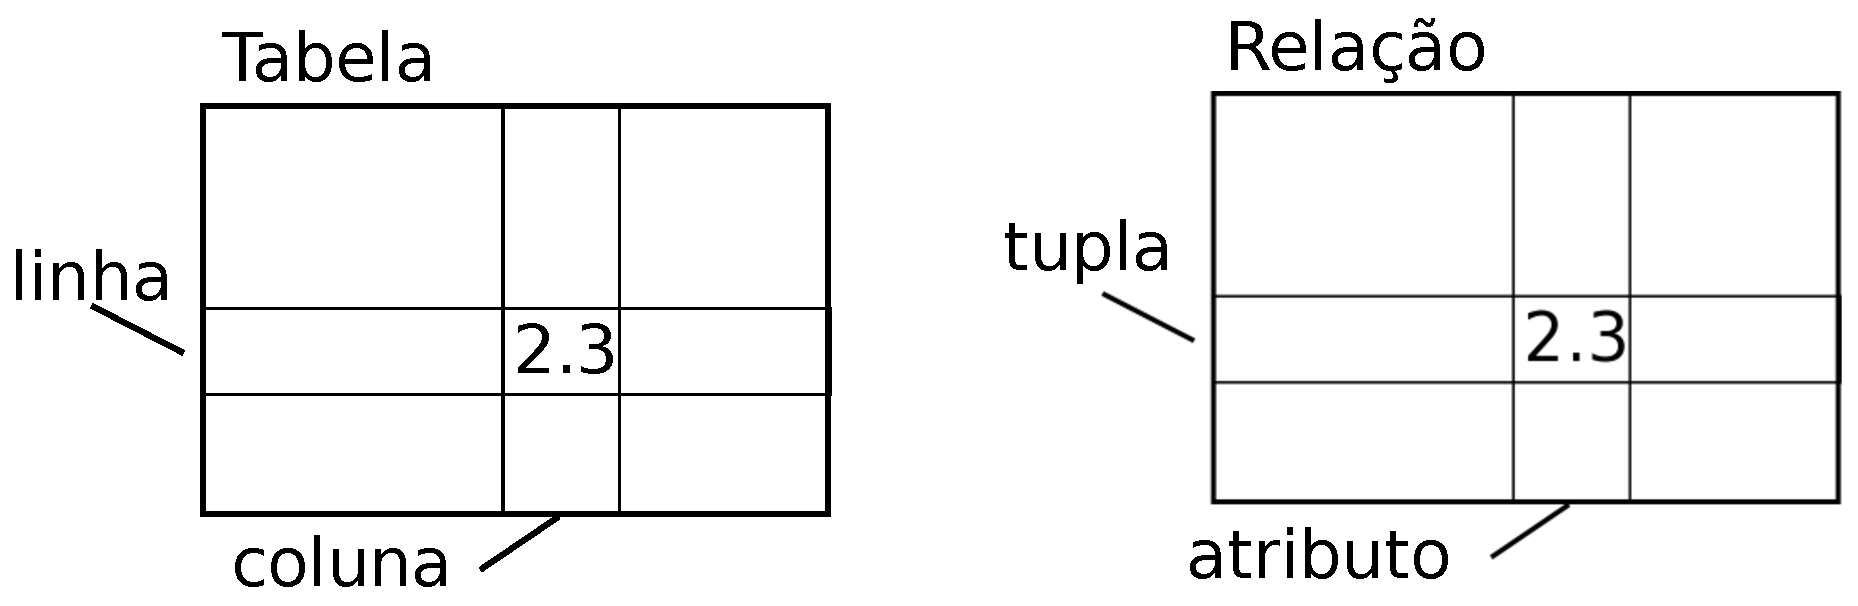
\includegraphics[height=1.50in]{figs2/relational.eps}}
\afterfig

%In technical descriptions of relational databases the concepts of 
%table, row, and column are more formally referred
%to as {\bf relation}, {\bf tuple}, and {\bf attribute}, respectively.
%We will use the less formal terms in this chapter.

Na descrição técnica de um banco de dados relacional o conceito de
tabela, linha e coluna são referências formais para {\bf relação},
{\bf tupla}, e {\bf atributo}, respectivamente.
Usaremos os termos menos formais neste capítulo.

%\section{SQLite manager Firefox add-on}
\section{Plugin do Firefox de Gerencia SQLite}
%While this chapter will focus on using Python to work with data 
%in SQLite database files, many operations can be done more
%conveniently using a Firefox add-on called the {\bf SQLite
%  Database Manager} which is freely available from:

O foco deste capítulo é o uso do Python para trabalhar com dados
com o SQLite, muitas operações podem ser feitas de forma mais
conveniente utilizando um {\it plugin} do Firefox, o {\bf SQLite
  Database Manager} que está disponível gratuitamente através do {\it link}:

\url{https://addons.mozilla.org/en-us/firefox/addon/sqlite-manager/}

%Using the browser you can easily create tables, insert data, edit data, 
%or run simple SQL queries on the data in the database.

Utilizando o navegador você pode facilmente criar tabelas, inserir, editar ou
executar consultas SQL nos dados da base de dados.

%In a sense, the database manager is similar to a text editor
%when working with text files.   When you want to do one or
%very few operations on a text file, you can just open it
%in a text editor and make the changes you want.   When you have 
%many changes that you need to do to a text file, often you 
%will write a simple Python program.  You will find the same 
%pattern when working with databases.  You will do simple
%operations in the database manager and more complex operations
%will be most conveniently done in Python.

De certa forma, o gerenciador de banco de dados é similar a um editor de texto
quando utilizado arquivos de texto. Quando você quer fazer uma ou mais
operações com um arquivo de texto, você pode simplesmente abrir o arquivo em
um editor de texto e fazer as alterações que desejar. Quando você tem que fazer
muitas alterações para fazer, normalmente você pode escrever um programa em
Python simples para executar esta tarefa. Você encontrará os mesmos padrões
quando for trabalhar com banco de dados. Você fará operações em um gerenciador
de banco de dados e as operações mais complexas serão mais convenientes se
forem feitas com Python.

%\section{Creating a database table}
\section{Criado uma tabela em um banco de dados}

%Databases require more defined structure than Python lists 
%or dictionaries\footnote{SQLite actually does allow some 
%flexibility in the type of data stored in a column,
%but we will keep our data types strict in this chapter
%so the concepts apply equally to other database systems 
%such as MySQL.}.

Bancos de dados precisam de estruturas mais bem definidas do quê listas ou
dicionários em Python\footnote{Atualmente o SQLite permite uma maior
  flexibilidade em relação aos tipos de dados que são armazenados em uma
  coluna, mas vamos manter os tipos de dados restritos neste capítulo, assim
  os mesmos conceitos aprendidos aqui podem ser aplicados a outros sistemas
  de banco de dados como MySQL.}.

%When we create a database {\bf table} we
%must tell the database in advance the names of each of the
%{\bf columns} in the table and the type of data which we are 
%planning to store in each {\bf column}.   When the database software
%knows the type of data in each column, it can choose the most 
%efficient way to store and look up the data based on the type of
%data.

Quando criamos uma {\bf tabela} em um banco de dados, precisamos informar ao
banco de dados previamente o nome de cada {\bf coluna} na tabela e o tipo de
dados que planejamos armazenar em cada {\bf coluna}. Quando o sistema de
banco de dados conhece o tipo de dado em cada coluna, ele pode definir a
forma mais eficiente de armazenar e consultar o dado baseado no tipo do dado.

%You can look at the various data types supported by SQLite
%at the following url:

Você pode visualizar os diversos tipos de dados que são suportados pelo SQLite
através do seguinte endereço:

\url{http://www.sqlite.org/datatypes.html}


%Defining structure for your data up front may seem inconvenient
%at the beginning, but the payoff is fast access to your data 
%even when the database contains a large amount of data.

Definir a estrutura dos seus tipos de dados pode parecer inconveniente no
começo, mas a recompensa é o acesso rápido aos dados mesmo quando o banco
de dados contém um grande número de informações.

%The code to create a database file and a table 
%named {\tt Tracks} with two columns in the 
%database is as follows:

O seguinte código cria um arquivo de banco de dados com uma tabela, chamada
{\tt Tracks} e com duas colunas:

\index{sqlite3 module}
\index{module!sqlite3}
\beforeverb
\begin{verbatim}
import sqlite3

conn = sqlite3.connect('music.sqlite3')
cur = conn.cursor()

cur.execute('DROP TABLE IF EXISTS Tracks ')
cur.execute('CREATE TABLE Tracks (title TEXT, plays INTEGER)')

conn.close()
\end{verbatim}
\afterverb
%
\index{connect function}
\index{function!connect}
\index{cursor function}
\index{function!cursor}
%The {\tt connect} operation makes a ``connection'' to the database 
%stored in the file {\tt music.sqlite3} in the current directory.   If
%the file does not exist, it will be created.  The reason this
%is called a ``connection'' is that sometimes the database is stored
%on a separate ``database server'' from the server on which we 
%are running our application.  In our simple examples 
%the database will just be a local file in the same directory
%as the Python code we are running.

A operação {\tt connect} cria uma ``conexão'' com o banco de dados armazenado
no arquivo {\tt music.sqlite3} no diretório corrente. Se o arquivo não
existir, este será criado. O motivo para isto ser chamado de ``conexão'' é
que algumas vezes o banco de dados está  em um ``servidor de banco de dados'' 
separado da aplicação propriamente dita. Em nossos exemplos o banco de dados
está armazenado localmente em um arquivo no mesmo diretório que o código
Python está sendo executado.


%A {\bf cursor} is like a file handle that we can use to perform
%operations on the data stored in the database.  Calling 
%{\tt cursor()} is very similar conceptually to calling
%{\tt open()} when dealing with text files.

Um {\bf cursos} é como um identificador de arquivo que podemos utilizar para
realizar operações sobre as informações armazenadas em um banco de dados. Ao
chamar a função {\tt cursor()}, conceitualmente, é similar ao chamar a função
{\tt open()} quando estamos trabalhando com arquivos de texto.

\beforefig
\centerline{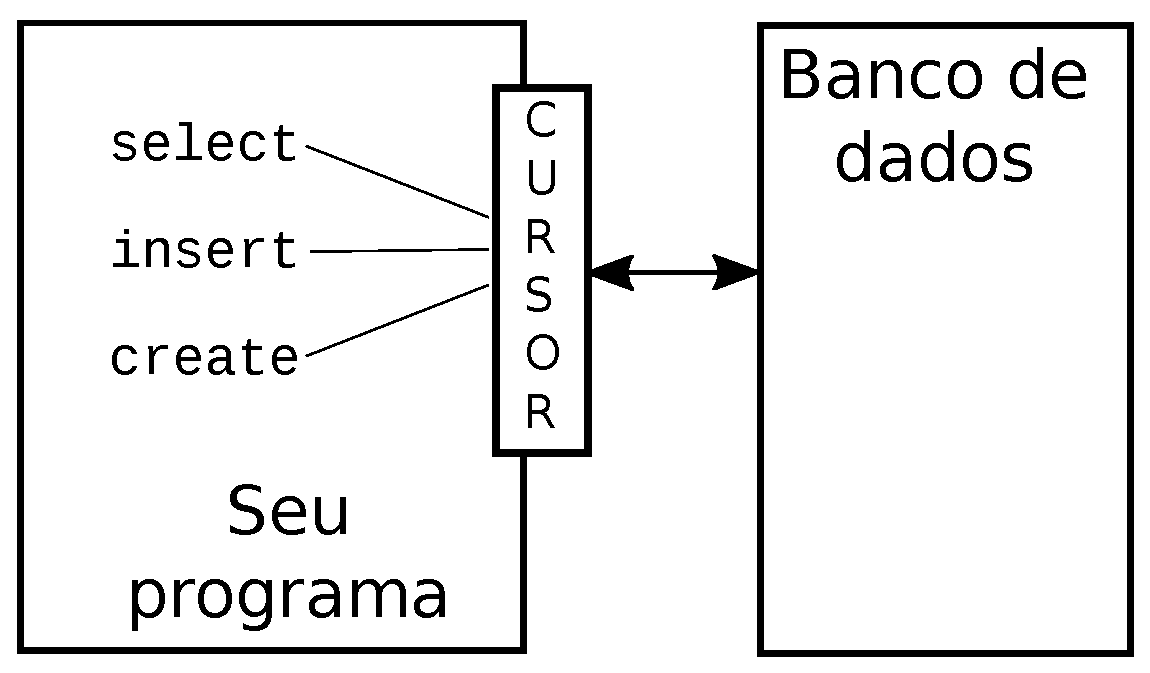
\includegraphics[height=1.50in]{figs2/cursor.eps}}
\afterfig

%Once we have the cursor, we can begin to execute 
%commands on the contents of the database using the {\tt execute()}
%method.

Uma vez que temos o cursos, podemos começar a executar comandos no conteúdo
armazenado no banco de dados utilizando o método {\tt execute()}.

%Database commands are expressed in a special language that has 
%been standardized across many different database vendors 
%to allow us to learn a single database language.   The database
%language is called {\bf Structured Query Language} or {\bf SQL}
%for short.

Os comandos de um banco de dados são expressos em uma linguagem especial que
foi padronizada por diferentes fornecedores de bancos de dados, que nos
permite aprender uma única linguagem. A linguagem dos bancos de dados é
chamada de {\bf Structured Query Language}\footnote{Em Português, pode ser
  chamada de Linguagem de Consulta Estruturada} ou referenciada pelo acrônimo
{\bf SQL}
\url{http://en.wikipedia.org/wiki/SQL}

%In our example, we are executing two SQL commands in our database.
%As a convention, we will show the SQL keywords in uppercase 
%and the parts of the command that we are adding (such as the
%table and column names) will be shown in lowercase.

Em nossos exemplos, estamos executando dois comandos SQL no banco de dados que
criamos. Convencionaremos que os comandos SQL serão mostrados em maiúsculas e
as partes que não são palavras reservadas do SQL (como os nomes das tabelas e
colunas) serão mostrados em minúsculas.

%The first SQL command removes the {\tt Tracks} table from the 
%database if it exists.  This pattern is simply to allow us to 
%run the same program to create the {\tt Tracks} table over 
%and over again without causing an error.  Note that the
%{\tt DROP TABLE} command deletes the table and all of its contents
%from the database (i.e., there is no ``undo'').

O primeiro comando SQL remove a tabela {\tt Tracks} do banco de dados se ela
existir. Este padrão nos permite executar o mesmo programa para criar a tabela
{\tt Tracks} repetidas vezes sem que cause erro. Perceba que o comando {\tt DROP
  TABLE} remove a tabela e todo o seu conteúdo do banco de dados (i.e., não é
possível desfazer esta operação)

\beforeverb
\begin{verbatim}
cur.execute('DROP TABLE IF EXISTS Tracks ')
\end{verbatim}
\afterverb
%
%The second command creates a table named
%{\tt Tracks} with a text column named {\tt title}
%and an integer column named {\tt plays}.
%
O segundo comando cria a tabela {\tt Tracks} com uma coluna chamada {\tt title}
com o tipo texto e uma coluna chamada {\tt plays} com o tipo inteiro.

\beforeverb
\begin{verbatim}
cur.execute('CREATE TABLE Tracks (title TEXT, plays INTEGER)')
\end{verbatim}
\afterverb
%
%Now that we have created a table named {\tt Tracks}, we can put some data
%into that table using the SQL {\tt INSERT} operation.   Again, we begin
%by making a connection to the database and obtaining the {\tt cursor}.
%We can then execute SQL commands using the cursor.
%
Agora que criamos a tabela {\tt Tracks}, podemos inserir algum dado dentro
dela utilizando a operação SQL {\tt INSERT}. Novamente, estamos
estabelecendo uma conexão com o banco de dados e obtendo o {\tt cursos}.
E então executamos o comando SQL utilizando o cursor.

%The SQL {\tt INSERT} command indicates which table we are using 
%and then defines a new row by listing the fields we want to 
%include {\tt (title, plays)} followed by the {\tt VALUES} we want
%placed in the new row.  We specify the values as question marks
%{\tt (?, ?)} to indicate that the actual values are passed in as a
%tuple {\tt ( 'My Way', 15 ) } as the second parameter to the
%{\tt execute()} call.

O comando SQL {\tt INSERT} indica qual tabela estamos utilizando, e em seguida, 
cria uma nova linha listando quais campos utilizaremos para incluir {\tt (title,
  plays)} seguido pelo comando {\tt VALUES} com os valores que desejamos
adicionar na nova linha. Especificamos os valores utilizando pontos de
interrogação {\tt (?, ?)} para indicar que os valores serão passados como
tuplas {\tt ( 'My Way', 15) } como um segundo parâmetro da chamada
{\tt execute()}.

\beforeverb
\begin{verbatim}
import sqlite3

conn = sqlite3.connect('music.sqlite3')
cur = conn.cursor()

cur.execute('INSERT INTO Tracks (title, plays) VALUES ( ?, ? )', 
    ( 'Thunderstruck', 20 ) )
cur.execute('INSERT INTO Tracks (title, plays) VALUES ( ?, ? )', 
    ( 'My Way', 15 ) )
conn.commit()

print 'Tracks:'
cur.execute('SELECT title, plays FROM Tracks')
for row in cur :
   print row

cur.execute('DELETE FROM Tracks WHERE plays < 100')
conn.commit()

cur.close()
\end{verbatim}
\afterverb
%
%First we {\tt INSERT} two rows into our table and use {\tt commit()} 
%to force the data to be written to the database file.

Primeiro nós adicionamos com {\tt INSERT} duas linha na nossa tabela e
usamos {\tt commit()} para forçar a escrita da informação no arquivo do banco
de dados.

\beforefig
\centerline{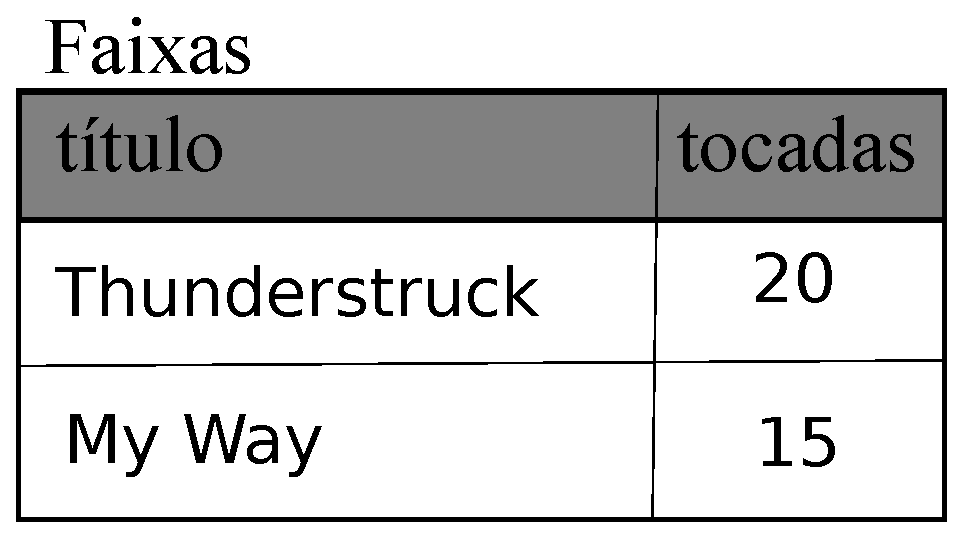
\includegraphics[height=1.00in]{figs2/tracks.eps}}
\afterfig

%Then we use the {\tt SELECT} command
%to retrieve the rows we just inserted from the table.  
%On the 
%{\tt SELECT} command, we indicate which columns we would like {\tt (title, plays)}
%and indicate which table we want to retrieve the data from.  After we 
%execute the {\tt SELECT} statement, the cursor is something we can loop through
%in a {\tt for} statement.   For efficiency,
%the cursor does not read all of the data from the
%database when we execute the {\tt SELECT} statement.  
%Instead, the data is read on demand
%as we loop through the rows in the {\tt for} statement.

Depois usamos o comando {\tt SELECT} para buscar a linha que acabamos de
inserir na tabela. Com o comando {\tt SELECT}, indicamos que coluna gostaríamos
{\tt (title, plays)} e de qual tabela queremos buscar a informação. Depois
de confirmar a executação do comando {\tt SELECT}, o cursor pode ser utilizado
como repetição através de um comando {\tt for}. Por questões de eficiência, o
cursor não lê toda a informação da base de dados quando executamos o comando
{\tt SELECT}. Ao invés disto, a informação é lida sob demanda enquanto
iteramos através da linha com o comando {\tt for}.

%The output of the program is as follows:

A saída do programa fica da seguinte forma:

\beforeverb
\begin{verbatim}
Tracks:
(u'Thunderstruck', 20)
(u'My Way', 15)
\end{verbatim}
\afterverb
%
\index{Unicode}
%Our {\tt for} loop finds two rows, and each row is a Python tuple with the
%first value as the {\tt title} and the second value as the number of {\tt plays}.
%Do not be concerned that the title strings are shown starting with 
%{\tt u'}.  This is an indication that the strings are {\bf Unicode} strings
%that are capable of storing non-Latin character sets.

A iteração do {\tt for} encontrou duas linhas, e cada linha é uma tupla em
Python com o primeiro valor como {\tt title} e o segundo como o número de
{\tt plays}. Não se preocupe com o fato de a {\it strings} são mostrados com
o caractere {\tt u'} no começo. Isto é uma indicação que a {\it string} estão
em {\bf Unicode}, o que indica que são capazes de armazenar um conjunto de
caractere não-Latin.

%At the very end of the program, we execute an SQL command to {\tt DELETE} 
%the rows we have just created so we can run the program over and over.
%The {\tt DELETE} command shows the use of a {\tt WHERE} clause that
%allows us to express a selection criterion so that we can ask the database
%to apply the command to only the rows that match the criterion.  In this example
%the criterion happens to apply to all the rows so we empty the table
%out so we can run the program repeatedly.  After the {\tt DELETE} is performed,
%we also call {\tt commit()} to force the data to be removed from the database.

No final do programa, executamos o comando SQL {\tt DELETE} para remover as
linhas que acabamos de criar, assim podemos executar o programa repetidas
vezes. O {\tt DELETE} pode ser utilizado com a condição {\tt WHERE} que permite
selecionar através de uma expressão o critério permitindo pesquisar no banco
de dados somente as linhas que correspondem com a expressão utilizada. Neste
exemplo a expressão construida se aplica em todas as linhas, para que possamos
executar o programa outras vezes. Depois de executar o {\tt DELETE} chamamos o
{\tt commit()} para forçar que o dado seja removido do banco de dados.

%\section{Structured Query Language summary}
\section{Resumo de Structured Query Language (SQL)}

%So far, we have been using the Structured Query Language in our Python
%examples and have covered many of the basics of the SQL commands.
%In this section, we look at the SQL language in particular
%and give an overview of SQL syntax.

Estamos utilizando SQL junto com os exemplos de Python e até agora cobrimos
muitos comandos SQL básicos. Nesta seção, vamos olhar a linguagem SQL com
mais atenção e apresentaremos uma visão geral da sintaxe do SQL.

%Since there are so many different database vendors, the Structured Query
%Language (SQL) was standardized so we could communicate in a portable
%manner to database systems from multiple vendors.

Existem diferentes fornecedores de bancos de dados, a linguagem SQL foi
padronizada, desta forma podemos nos comunicar de maneira portável entre os
diferentes sistemas de banco de dados dos diferentes fornecedores.

%A relational database is made up of tables, rows, and columns.  The columns
%generally have a type such as text, numeric, or date data.  When we create
%a table, we indicate the names and types of the columns:

Basicamente um banco de dados relacional é composto por tabelas, linhas e
colunas. As colunas geralmente possuem tipos, como textos, números ou
informação de data. Quando criamos uma tabela, indicamos os nomes e tipos das
colunas:

\beforeverb
\begin{verbatim}
CREATE TABLE Tracks (title TEXT, plays INTEGER)
\end{verbatim}
\afterverb
%
%To insert a row into a table, we use the SQL {\tt INSERT} command:
%
Para inserir uma linha em uma tabela, utilizamos o comando SQL {\tt INSERT}:

\beforeverb
\begin{verbatim}
INSERT INTO Tracks (title, plays) VALUES ('My Way', 15)
\end{verbatim}
\afterverb
%
%The {\tt INSERT} statement specifies the table name, then a list of
%the fields/columns that you would like to set in the new row, and then 
%the keyword {\tt VALUES} and a list of corresponding values 
%for each of the fields.
%
A declaração do {\tt INSERT} especifica o nome da tabela, e então, uma lista
dos campos/colunas que gostaríamos de definir na nova linha, e por fim,
através do campo {\tt VALUES} passamos uma lista de valores correspondentes a
cada campo.

%The SQL {\tt SELECT} command is used to retrieve rows and columns from a database.
%The {\tt SELECT} statement lets you specify which columns you would
%like to retrieve as well as a {\tt WHERE} clause to select which 
%rows you would like to see.  It also allows an optional 
%{\tt ORDER BY} clause to control the sorting of the returned rows.

O comando {\tt SELECT} é utilizado para buscar as linhas e colunas de um banco
de dados. A declaração do {\tt SELECT} permite que você especifique qual coluna
gostaria de buscar, bem como utilizando a condição do {\tt WHERE}, permite
selecionar qual linha gostaríamos de visualizar. Isto também possibilita o uso
de uma condição opcional, {\tt ORDER BY}, para ordenar as linhas retornadas.

\beforeverb
\begin{verbatim}
SELECT * FROM Tracks WHERE title = 'My Way'
\end{verbatim}
\afterverb
%
%Using \verb"*" indicates that you want the database to return all of 
%the columns for each row that matches the {\tt WHERE} clause.

O uso do \verb"*" indica que o banco de dados deve retornar todas as colunas
para cada linha que casa com a condição {\tt WHERE}.

%Note, unlike in Python, in a SQL {\tt WHERE} clause 
%we use a single equal sign 
%to indicate a test for equality rather than a double equal sign.
%Other logical operations allowed in a {\tt WHERE} clause include

Atenção, diferente de Python, a condição {\tt WHERE}, em SQL, utiliza o sinal
de igual simples (\verb"="), para indicar uma condição de igualdade, ao invés de
um sinal duplo (\verb"==")
\verb"<",
\verb">",
\verb"<=",
\verb">=",
\verb"!=",
%as well as {\tt AND} and {\tt OR} and parentheses
%to build your logical expressions.

assim como é possível utilizar as condições {\tt AND} e {\tt OR} e parênteses
para construir expressões lógicas.

%You can request that the returned rows be sorted by one of 
%the fields as follows:

Você pode pedir que as linhas retornadas sejam ordenadas por um dos campos
como apresentados no exemplo a seguir:
\beforeverb
\begin{verbatim}
SELECT title,plays FROM Tracks ORDER BY title
\end{verbatim}
\afterverb
%
%To remove a row, you need a {\tt WHERE} clause on an SQL {\tt DELETE}
%statement.  The {\tt WHERE} clause determines which rows are to be deleted:
%
Para remover uma linha, é preciso combinar a condição {\tt WHERE} com a
condição {\tt DELETE}. O {\tt WHERE} irá determinar quais linhas serão
removidas:

\beforeverb
\begin{verbatim}
DELETE FROM Tracks WHERE title = 'My Way'
\end{verbatim}
\afterverb
%
%It is possible to {\tt UPDATE} a column or columns within one or more rows
%in a table using the SQL {\tt UPDATE} statement as follows:
%
É possível alterar/atualizar uma ou mais colunas e suas linhas de uma tabela
utilizando a condição SQL {\tt UPDATE}, da seguinte forma:

\beforeverb
\begin{verbatim}
UPDATE Tracks SET plays = 16 WHERE title = 'My Way'
\end{verbatim}
\afterverb
%
%The {\tt UPDATE} statement specifies a table and 
%then a list of fields and values to change after the {\tt SET} 
%keyword and then an optional {\tt WHERE} clause to select
%the rows that are to be updated.  A single {\tt UPDATE} statement
%will change all of the rows that match the {\tt WHERE} clause.  If 
%a {\tt WHERE} clause is not specified, it performs the {\tt UPDATE}
%on all of the rows in the table.
%
A condição {\tt UPDATE} especifica uma tabela e depois uma lista de campos e
valores que serão alterados após o comando {\tt SET}, e utilizando uma condição
{\tt WHERE}, opctional, é possível selecionar as linhas que serão atualizadas.
Uma condição {\tt UPDATE} irá mudar todas as linhas que casam com a condição
{\tt WHERE}. Se a condição {\tt WHERE} não for especificada, o {\tt UPDATE}
será aplicado em todas as linhas da tabela.

%These four basic SQL commands (INSERT, SELECT, UPDATE, and DELETE) allow 
%the four basic operations needed to create and maintain data.

Os quatros comandos básicos de SQL (INSERT, SELECT, UPDTE e DELETE) permitem
as quatro operações básicas necessárias para criação e manutenção das
informações em um banco de dados.

%\section{Spidering Twitter using a database}
\section{Rastreando o Twitter utilizando um banco de dados}

%In this section, we will create a simple spidering program that will 
%go through Twitter accounts and build a database of them.
%\emph{Note: Be very careful when running this program.  You do not
%want to pull too much data or run the program for too long and
%end up having your Twitter access shut off.}

Nesta seção criaremos um programa simples para rastreamento que navegará
através de contas de usuários do Twitter e construirá um banco de dados
destas referentes as estes usuários.
\emph{Nota: Tenha muito cuidado ao executar este programa. Você não irá querer
  extrair muitas informações ou executar o programa por muito tempo e acabar
  tendo sua conta do Twitter bloqueada.}

%One of the problems of any kind of spidering program is that it 
%needs to be able to be stopped and restarted many times and 
%you do not want to lose the data that you have retrieved so far.
%You don't want to always restart your data retrieval at the
%very beginning so we want to store data as we retrieve it so our
%program can start back up and pick up where it left off.

Um dos problemas, em qualquer tipo de programas de rastreamento, é que precisa
ser capaz de ser interrompido e reiniciado muitas vezes e você não quer perder
informações que você já tenha recuperado até agora. Não quer sempre reiniciar
a recuperação dos dados desde o começo, então armazenamos as informações tão
logo seja recuperada, assim o programa poderá reiniciar a busca do ponto onde
parou.


%We will start by retrieving one person's Twitter friends and their
%statuses, looping through the list of friends, and adding each 
%of the friends to a database to be retrieved in the future.  After
%we process one person's Twitter friends, we check in our database
%and retrieve one of the friends of the friend.  We do this over and
%over, picking an ``unvisited'' person, retrieving their friend list,
%and adding friends we have not seen to our list for a future visit.

Vamos começar recuperando os amigos de uma pessoa no Twitter e seus status,
iterando na lista de amigos, e adicionando cada um ao banco de dados para
que possa ser recuperado no futuro. Depois de listar os amigos de uma pessoa,
verificamos na nossa base de dados e coletamos os amigos de um dos amigos da
primeira pessoa. Vamos fazendo isto repetidas vezes, escolhendo umas das
pessoas ``não visitadas'', recuperando sua lista de amigos, e
adicionando amigos que não tenhamos visto anteriormente a nossa lista, para
visitar futuramente.

%We also track how many times we have seen a particular friend in the
%database to get some sense of their ``popularity''.

Também rastrearemos quantas vezes vimos um amigo em particular na nossa base
para ter uma ideia da sua ``popularidade''.

%By storing our list of known accounts and whether 
%we have retrieved the account or not, 
%and how popular the account is in a database on the disk
%of the computer, we can stop and
%restart our program as many times as we like.

Armazenando nossa lista de contas conhecidas, no banco de dados no disco do
nosso computador, e se já recuperamos a conta ou não, e quanto esta conta é
popular, podemos parar e recomeçar nosso programa quantas vezes quisermos.

% TODO: Add a reference to the right spot
%This program is a bit complex. It is based on the code 
%from the exercise earlier in the book that uses
%the Twitter API.

% TODO: Adicionar a referência do código para o lugar certo.
Este programa é um pouco complexo. É baseado em um exercício apresentado
anteriormente neste livro, que utiliza a API do Twitter

%Here is the source code for our Twitter spidering application:

O seguinte código apresenta o programa que realiza o rastreamento no Twitter:

\beforeverb
\begin{verbatim}
import urllib
import twurl
import json
import sqlite3

TWITTER_URL = 'https://api.twitter.com/1.1/friends/list.json'

conn = sqlite3.connect('spider.sqlite3')
cur = conn.cursor()

cur.execute('''
CREATE TABLE IF NOT EXISTS Twitter 
(name TEXT, retrieved INTEGER, friends INTEGER)''')

while True:
    acct = raw_input('Enter a Twitter account, or quit: ')
    if ( acct == 'quit' ) : break
    if ( len(acct) < 1 ) :
        cur.execute('SELECT name FROM Twitter WHERE retrieved = 0 LIMIT 1')
        try:
            acct = cur.fetchone()[0]
        except:
            print 'No unretrieved Twitter accounts found'
            continue

    url = twurl.augment(TWITTER_URL, 
               {'screen_name': acct, 'count': '20'} )
    print 'Retrieving', url
    connection = urllib.urlopen(url)
    data = connection.read()
    headers = connection.info().dict
    # print 'Remaining', headers['x-rate-limit-remaining']
    js = json.loads(data)
    # print json.dumps(js, indent=4)

    cur.execute('UPDATE Twitter SET retrieved=1 WHERE name = ?', (acct, ) )

    countnew = 0
    countold = 0
    for u in js['users'] :
        friend = u['screen_name']
        print friend
        cur.execute('SELECT friends FROM Twitter WHERE name = ? LIMIT 1', 
            (friend, ) )
        try:
            count = cur.fetchone()[0]
            cur.execute('UPDATE Twitter SET friends = ? WHERE name = ?', 
                (count+1, friend) )
            countold = countold + 1
        except:
            cur.execute('''INSERT INTO Twitter (name, retrieved, friends) 
                VALUES ( ?, 0, 1 )''', ( friend, ) )
            countnew = countnew + 1
    print 'New accounts=',countnew,' revisited=',countold
    conn.commit()

cur.close()
\end{verbatim}
\afterverb
%
%Our database is stored in the file {\tt spider.sqlite3} and it has one 
%table named {\tt Twitter}.  Each row in the {\tt Twitter} table
%has a column for the account name, whether we have retrieved the friends
%of this account, and how many times this account has been ``friended''.

%
Nossa base de dados está armazenada no arquivo {\tt spider.sqlite3} e possui
uma tabela chamada {\tt Twitter}. Cada linha na tabela {\tt Twitter} tem uma
coluna para o nome da conta, se recuperamos os amigos desta conta, e quantas
vezes esta conta foi ``seguido''.

%In the main loop of the program, we prompt the user for a Twitter
%account name or ``quit'' to exit the program.  
%If the user enters a Twitter account, we retrieve the 
%list of friends and statuses
%for that user and add each friend to the database if 
%not already in the database.  If the friend is already in the list, 
%we add 1 to the {\tt friends} field in the row in the database.

Na repetição principal do programa, perguntamos ao usuário uma conta de Twitter
ou ``quit'' para sair do programa. Se o usuário informar um usuário do Twitter,
o programa começa a recuperar a lista de amigos e os status para aquele
usuário e adiciona cada amigo na base de dados se não possuir. Se o amigo já
está na lista, nós adicionamos ``1'' no campo {\tt friends} da base de dados.


%If the user presses enter, we look in the database for the next 
%Twitter account that we have not yet retrieved, retrieve the
%friends and statuses for that account, add them to the database 
%or update them, and increase their {\tt friends} count.

Se o usuário pressionar {\tt enter}, pesquisamos na base a próxima conta que
não rastreamos ainda, e então rastreamos os amigos e status com aquela conta
e adicionamos na base de dados ou atualizamos, incrementando seu contador de
{\tt friends}.

%Once we retrieve the list of friends and statuses, we loop 
%through all of the {\tt user} items in the returned JSON
%and retrieve the \verb"screen_name" for each user.  Then we use
%the {\tt SELECT} statement to see if we already have stored this
%particular \verb"screen_name" in the database and retrieve the
%friend count ({\tt friends}) if the record exists.

Uma vez que rastreamos a lista de amigos e status, iteramos entre todas os
ítens {\tt user} retornados no JSON e rastreamos o  \verb"screen_name" para
cada usuário. Então utilizamos a declaração {\tt SELECT} para ver se já
armazenamos este \verb"screen_name" em particular na base e recuperamos o
contador de amigos ({\tt friends}), se este registro existir.

\beforeverb
\begin{verbatim}
    countnew = 0
    countold = 0
    for u in js['users'] :
        friend = u['screen_name']
        print friend
        cur.execute('SELECT friends FROM Twitter WHERE name = ? LIMIT 1', 
            (friend, ) )
        try:
            count = cur.fetchone()[0]
            cur.execute('UPDATE Twitter SET friends = ? WHERE name = ?', 
                (count+1, friend) )
            countold = countold + 1
        except:
            cur.execute('''INSERT INTO Twitter (name, retrieved, friends) 
                VALUES ( ?, 0, 1 )''', ( friend, ) )
            countnew = countnew + 1
    print 'New accounts=',countnew,' revisited=',countold
    conn.commit()
\end{verbatim}
\afterverb
%
%Once the cursor executes the {\tt SELECT} statement, 
%we must retrieve the rows.  We could do this with a {\tt for} 
%statement, but since we are only retrieving
%one row ({\tt LIMIT 1}), we can use the {\tt fetchone()} method to fetch the
%first (and only) row that is the result of the {\tt SELECT} operation.  
%Since {\tt fetchone()} returns the row as a {\bf tuple} (even though there is only
%one field), we take the first value from the tuple using {\tt [0]} to get the 
%current friend count into the variable {\tt count}.  

%
Uma vez que o cursor tenha executado o {\tt SELECT}, nós devemos recuperar as
linhas. Podemos fazer isto com uma declaração de {\tt for}, mas uma vez que
estamos recuperando uma linha ({\tt LIMIT 1}), podemos utilizar o método
{\tt fetchone()} para buscar a primeira (e única) linha que é o resultado da
operação {\tt SELECT}. Sendo o retorno {\tt fetchone()} uma linha como uma
{\bf tupla} (ainda que haja somente um campo), pegamos o primeiro valor da
tupla utilizando índice {\tt [0]} para pegar o contador de amigos atual dentro
da variável {\tt count}.

%If this retrieval is successful, we use the SQL {\tt UPDATE} statement with a 
%{\tt WHERE} clause to add 1 to the {\tt friends} column for the row that 
%matches the friend's account.  Notice that there are two placeholders (i.e.,
%question marks) in the SQL, and the second parameter to the {\tt execute()} is
%a two-element tuple that holds the values to be substituted into the SQL
%in place of the question marks.

Se a busca for bem sucedida, utilizamos a declação {\tt UPDATE} com a clausula 
{\tt WHERE} para adicionar 1 na coluna {\tt friends} para a linha que
corresponde com a conta do amigo. Note que existem dois espaços reservados
(i.e., pontos de interrogações) no SQL, e o segundo parâmetro para o
{\tt execute()} é uma tupla que armazena o valor para substituir no SQL no
lugar dos pontos de interrogações.

%If the code in the {\tt try} block fails, it is probably because no record
%matched the {\tt WHERE name = ?} clause on the SELECT statement.  So in the
%{\tt except} block, we use the SQL {\tt INSERT} statement to add the friend's
%\verb"screen_name" to the table with an indication that we have not yet 
%retrieved the \verb"screen_name" and set the friend count to zero.

Se o bloco {\tt try} falhar, é provavelmente por que nenhum resultado
corresponde a clausula em {\tt WHERE name = ?} do SELECT. Então no block
{\tt except}, utilizamos a declaração {\tt INSERT} para adicionar o
\verb"screen_name" do amigo a tabela com a indicação que ainda não rastreamos
o \verb"screen_name" e setamos o contador de amigos com 0 (zero).

%So the first time the program runs and we enter a Twitter account, the program
%runs as follows:

Assim, a primeira vez que o programa é executado e informamos uma conta do
Twitter, a saída do programa é a seguinte:

\beforeverb
\begin{verbatim}
Enter a Twitter account, or quit: drchuck
Retrieving http://api.twitter.com/1.1/friends ...
New accounts= 20  revisited= 0
Enter a Twitter account, or quit: quit
\end{verbatim}
\afterverb
%
%Since this is the first time we have run the program, the database
%is empty and we create the database in the file {\tt spider.sqlite3} and
%add a table named {\tt Twitter} to the database.  Then we retrieve
%some friends and add them all to the database since the database is
%empty.

Como esta é a primeira vez que executamos o programa, o banco de dados está
vazio e criamos o banco no arquivo {\tt spider.sqlite3}, adicionamos a tabela
chamada {\tt Twitter} na base de dados. Então nós rastreamos alguns amigos e
os adicionamos a base, uma vez que ela está vazia.

%At this point, we might want to write a simple database dumper
%to take a look at what is in our {\tt spider.sqlite3} file:

Neste ponto podemos escrever um {\it dumper} simples para olhar o que está no
nosso arquivo {\tt spider.sqlite3}:

\beforeverb
\begin{verbatim}
import sqlite3

conn = sqlite3.connect('spider.sqlite3')
cur = conn.cursor()
cur.execute('SELECT * FROM Twitter')
count = 0
for row in cur :
   print row
   count = count + 1
print count, 'rows.'
cur.close()
\end{verbatim}
\afterverb
%
%This program simply opens the database and selects all of the 
%columns of all of the rows in the table {\tt Twitter}, then 
%loops through the rows and prints out each row.

%
Este programa abre o banco de dados e seleciona todas as colunas de todas as
linhas na tabela {\tt Twitter}, depois itera em cada linha e imprime o valor
dentro de cada uma.

%If we run this program after the first execution of our Twitter
%spider above, its output will be as follows:

Se executarmos este programa depois da primeira execução do nosso rastreador
{\it spider} do Twitter, sua saída será como a seguinte:

\beforeverb
\begin{verbatim}
(u'opencontent', 0, 1)
(u'lhawthorn', 0, 1)
(u'steve_coppin', 0, 1)
(u'davidkocher', 0, 1)
(u'hrheingold', 0, 1)
...
20 rows.
\end{verbatim}
\afterverb
%
%We see one row for each \verb"screen_name", that we 
%have not retrieved the data for that \verb"screen_name", and 
%everyone in the database has one friend.

%
Veremos uma linha para cada \verb"screen_name", que não tenhamos recuperado
o dado daquele \verb"screen_name", e todos tem um amigo.

%Now our database reflects the retrieval of the friends of 
%our first Twitter account ({\bf drchuck}).  We can run the program
%again and tell it to retrieve the friends of the next 
%``unprocessed'' account by simply pressing enter instead of
%a Twitter account as follows:

Agora nosso banco de dados reflete quais amigos estão relacionados com a nossa
primeira conta do Twitter ({\bf drchuck}) utilizada para rastreamento. Podemos
executar o programa novamente e mandar rastrear a próxima conta
``não processada'' e recuperar os amigos, simplemente pressionando {\tt enter}
ao invés de informar uma conta do Twitter, conforme o exemplo a seguir:


\beforeverb
\begin{verbatim}
Enter a Twitter account, or quit: 
Retrieving http://api.twitter.com/1.1/friends ...
New accounts= 18  revisited= 2
Enter a Twitter account, or quit: 
Retrieving http://api.twitter.com/1.1/friends ...
New accounts= 17  revisited= 3
Enter a Twitter account, or quit: quit
\end{verbatim}
\afterverb
%
%Since we pressed enter (i.e., we did not specify a Twitter account),
%the following code is executed:

%
Uma vez que pressionamos {\tt enter} (i.e., não especificamos uma conta do
Twitter), o seguinte código é executado:

\beforeverb
\begin{verbatim}
    if ( len(acct) < 1 ) :
        cur.execute('SELECT name FROM Twitter WHERE retrieved = 0 LIMIT 1')
        try:
            acct = cur.fetchone()[0]
        except:
            print 'No unretrieved twitter accounts found'
            continue
\end{verbatim}
\afterverb
%
%We use the SQL {\tt SELECT} statement to retrieve the name of the first 
%({\tt LIMIT 1}) user who still has their ``have we retrieved this user''
%value set to zero.  We also use the {\tt fetchone()[0]} pattern within 
%a try/except block to either extract a \verb"screen_name" from the retrieved
%data or put out an error message and loop back up.

%
Utilizamos a declaração SQL {\tt SELECT} para recuperar o nome do primeiro
({\tt LIMIT 1}) usuário que ainda tem seu ``recuperamos este usuário'' com o
valor setado em zero. Também utilizamos o padrão {\tt fetchone()[0]} dentro de
um bloco try/except para extrair também um \verb"screen_name" do dado
recuperado ou apresentamos uma mensagem de erro e iteramos novamente.

%If we successfully retrieved an unprocessed \verb"screen_name", we retrieve
%their data as follows:

Se tivermos sucesso ao recuperar um \verb"screen_name" não processado, vamos
extrair seus dados da seguinte maneira:

\beforeverb
\begin{verbatim}
    url = twurl.augment(TWITTER_URL, {'screen_name': acct, 'count': '20'} )
    print 'Retrieving', url
    connection = urllib.urlopen(url)
    data = connection.read()
    js = json.loads(data)

    cur.execute('UPDATE Twitter SET retrieved=1 WHERE name = ?', (acct, ) )
\end{verbatim}
\afterverb
%
%Once we retrieve the data successfully, we use the {\tt UPDATE} statement 
%to set the {\tt retrieved} column to 1 to indicate that we have completed 
%the retrieval of the friends of this account.  This keeps us from retrieving
%the same data over and over and keeps us progressing forward through the network
%of Twitter friends.
%
Ao recuperar os dados com sucesso, utilizaremos a declaração {\tt UPDATE} para
setar a coluna {\tt retrieved} para 1 para indicar que completamos a extração
dos amigos relacionados com esta conta. Isto no permite recuperar o mesmo dado
diversas vezes e nos permite prosseguir através da lista de amigos no Twitter. 

%If we run the friend program and press enter twice to retrieve the next 
%unvisited friend's friends,
%then run the dumping program, it will give us the following output:

Se executarmos o programa novamente, e pressionarmos {\tt enter} duas vezes
seguidas para recuperar os próximos amigos do amigo e depois executarmos o
programa de {\it dumping}, ele nos mostrará a seguinte saída:

\beforeverb
\begin{verbatim}
(u'opencontent', 1, 1)
(u'lhawthorn', 1, 1)
(u'steve_coppin', 0, 1)
(u'davidkocher', 0, 1)
(u'hrheingold', 0, 1)
...
(u'cnxorg', 0, 2)
(u'knoop', 0, 1)
(u'kthanos', 0, 2)
(u'LectureTools', 0, 1)
...
55 rows.
\end{verbatim}
\afterverb
%
%We can see that we have properly recorded that we have visited 
%{\tt lhawthorn} and {\tt opencontent}.  Also the accounts 
%{\tt cnxorg} and {\tt kthanos} already have two followers.
%Since we now have retrieved the friends of three people
%({\tt drchuck}, {\tt opencontent}, and {\tt lhawthorn}) our table has 55 rows 
%of friends to retrieve.

Podemos ver que gravamos de forma apropriada que visitamos os usuários
{\tt lhawthorn} e {\tt opencontent}. E que as contas {\tt cnxorg} e
{\tt kthanos} já tem dois seguidores. Desde que tenhamos recuperado os amigos
de três pessoas ({\tt drchuck}, {\tt opencontent}, e {\tt lhawthorn}) nossa
tabela tem agora 55 linhas de amigos recuperados.

%Each time we run the program and press enter it will pick the next 
%unvisited account (e.g., the next account will be \verb"steve_coppin"),
%retrieve their friends, mark them as retrieved, and for each of the 
%friends of \verb"steve_coppin" either add them to the end of the 
%database or update their friend count if they are already in the
%database.

Cada vez que executamos o programa e pressionamos {\tt enter} ele pegará a
próxima conta não visitada (e.g., a próxima conta será \verb"steve_coppin"),
recuperar seus amigos, marcá-los como recuperados, e para cada um dos amigos
de \verb"steve_coppin" também adicionaremos eles para no fim da base de dados 
e atualizaremos seus amigos que já estiverem na base de dados.

%Since the program's data is all stored on disk in a database, 
%the spidering activity can be suspended and resumed as many times as you 
%like with no loss of data.

Assim que os dados do programa estejam armazenados no disco em um banco de
dados o rastreamento pode ser suspenso e reiniciado tantas vezes quando
quiser sem a perda de informações.

%\section{Basic data modeling}
\section{Modelagem de dados básica}

%The real power of a relational database is when we create multiple tables
%and make links between those tables.   The act of deciding how to break
%up your application data into multiple tables and establishing the
%relationships between the tables is called {\bf data modeling}.  The
%design document that shows the tables and their relationships 
%is called a {\bf data model}.

O verdadeiro poder de um banco de dados relacional é quando criamos múltiplas
tabelas e criamos ligações entre elas. Decidir como dividir os dados da sua
aplicação em diferentes tabelas e estabelecer a relação entre estas tabelas é
o que chamamos de {\bf modelagem de dados}. O documento que mostra a estrutura 
das tabelas e suas relações é chamado de {\bf modelo de dados}.

%Data modeling is a relatively sophisticated skill and we will only introduce
%the most basic concepts of relational data modeling in this section.  For more
%detail on data modeling you can start with:

Modelagem de dados é uma habilidade relativamente sofisticada e nesta seção
nós iremos somente introduzir os conceitos mais básicos da modelagem de dados
relacionais. Para maiores detalhes sobre modelagem de dados você pode começar
com:

\url{http://en.wikipedia.org/wiki/Relational_model}

%Let's say for our Twitter spider application, instead of just
%counting a person's friends, we wanted to keep a list of 
%all of the incoming relationships so we could find a list of 
%everyone who is following a particular account.

Digamos que para a nossa aplicação de rastreamento do Twitter, ao invés de
só contar os amigos das pessoas, nós queiramos manter uma lista de todas as
relações de entrada, então poderemos encontrar uma lista de todos que seguem
uma pessoa em particular.

%Since everyone will potentially have many accounts that follow
%them, we cannot simply add a single column to our {\tt Twitter} table. 
%So we create a new table that keeps track of pairs of friends.
%The following is a simple way of making such a table:

Já que todos, potencialmente, terão tantas contas que o sigam, nós não podemos
simplesmente adicionar uma coluna para nossa tabela {\tt Twitter}. Então
criamos uma nova tabela que mantém o controle dos pares de amigos. A seguir
temos uma forma simples de criar tal tabela:

\beforeverb
\begin{verbatim}
CREATE TABLE Pals (from_friend TEXT, to_friend TEXT)
\end{verbatim}
\afterverb
%
%Each time we encounter a person who {\tt drchuck} is following, we
%would insert a row of the form:
%
Toda vez que encontrarmos uma pessoa que {\tt drchuck} está seguindo, nós
iremos inserir uma linha da seguinte forma:

\beforeverb
\begin{verbatim}
INSERT INTO Pals (from_friend,to_friend) VALUES ('drchuck', 'lhawthorn')
\end{verbatim}
\afterverb
%
%As we are processing the 20 friends from the {\tt drchuck}
%Twitter feed, we will insert 20 records with ``drchuck''
%as the first parameter so we will end up duplicating the 
%string many times in the database.
%
Como estamos processando 20 amigos da conta do {\it Twitter} do {\tt drchuck},
inserimor 20 registros com ``drchuck'' como primeiro parâmetro e assim
acaberemos duplicando a {\it string} muitas vezes no banco de dados.

%This duplication of string data violates one of the best practices 
%for {\bf database normalization} which basically states that
%we should never put the same string data in the database more than once.  
%If we need the data more than once, we create a 
%numeric {\bf key} for the data and reference the actual data 
%using this key.

Esta duplicação de dados viola uma das melhores práticas da {\bf normatização
  de banco de dados} que basicamente afirma que nunca devemos colocar o mesmo
dado mais de uma vez em um banco de dados. Se precisarmos inserir um dado mais
de uma vez, criamos uma referência numérica {\bf key} (chave) para o dado, e
utilizamos a chave para referenciar o dado.

%In practical terms, a string takes up a lot more 
%space than an integer on the disk
%and in the memory of our computer, and takes more processor time
%to compare and sort.  If we only have a few hundred entries, 
%the storage and processor time hardly matters.  But if we have 
%a million people in our database and a possibility of 100 million
%friend links, it is important to be able to scan data as quickly
%as possible.

Na prática, uma {\it string} ocupa muito mais espaço do que um inteiro, no
disco e na memória do nosso computador, e leva mais tempo do processor para
comparar e ordenar. Se tivermos somente algumas centenas de entradas, a base
de dados e o tempo de processamento dificilmente importarão. Mas se tivermos
um milhão de pessoas na nossa base de dados e uma possibilidade de 100 milhões
de conexões de amigos, é importante permitir examinar os dados o mais rápido
possível.

%We will store our Twitter accounts in a table named {\tt People}
%instead of the {\tt Twitter} table used in the previous example.
%The {\tt People} table has an additional column 
%to store the numeric key associated with the 
%row for this Twitter user.   
%SQLite has a feature that automatically adds the key value
%for any row we insert into a table using a special type of 
%data column ({\tt INTEGER PRIMARY KEY}).

Nós armazenaremos nossas contas do Twitter em uma tabela chamada {\tt People}
ao invés de utilizar a tabela {\tt Twitter} utilizada no exemplo anterior. A
tabela {\tt People} tem uma coluna adicional para armazenar uma chave associada
a linha para este usuário.

%We can create the {\tt People} table with this additional 
%{\tt id} column as follows:

Podemos criar a tabela {\tt People} com esta coluna {\tt id} adicional com o
seguinte comando:

\beforeverb
\begin{verbatim}
CREATE TABLE People 
    (id INTEGER PRIMARY KEY, name TEXT UNIQUE, retrieved INTEGER)
\end{verbatim}
\afterverb
%
%Notice that we are no longer maintaining a friend count in each row
%of the {\tt People} table.
%When we select {\tt INTEGER PRIMARY KEY} as the type of our {\tt id} column,
%we are indicating that we would like SQLite to manage this column and 
%assign a unique numeric key to each row we insert automatically.
%We also add the keyword {\tt UNIQUE} to indicate that we will not 
%allow SQLite to insert two rows with the same value for {\tt name}.
%
Perceba que nós não estamos mais mantendo uma conta de amigo em cada linha da
tabela {\tt People}. Quando selecionamos {\tt INTEGER PRIMARY KEY} como o tipo
da nossa coluna {\tt id}, estamos indicando que gostaríamos que o SQLite
gerencie esta coluna e defina uma chave numérica única automagicamente para
cada linha que inserirmos. Também adicionamos uma palavra-chave {\tt UNIQUE}
para indicar que não permitiremos ao SQLite inserir duas linhas com o mesmo
valor para {\tt name}.

%Now instead of creating the table {\tt Pals} above, we create
%a table called {\tt Follows} with two integer columns
%\verb"from_id" and \verb"to_id" and a constraint on the table that
%the \emph{combination} of \verb"from_id" and \verb"to_id" must be unique 
%in this table (i.e., we cannot insert duplicate rows) in our database.

Agora, ao invés de criar a tabela {\tt Pals} acima, criaremos uma tabela
chamada {\tt Follows} com duas colunas com o tipo inteiro \verb"from_id" e
\verb"to_id" e associaremos na tabela onde a \emph{combinação} de
\verb"from_id" e \verb"to_id" devem ser únicos nesta tabela (i.e., não podemos
inserir linhas duplicadas) na nossa base de dados.

\beforeverb
\begin{verbatim}
CREATE TABLE Follows 
    (from_id INTEGER, to_id INTEGER, UNIQUE(from_id, to_id) )
\end{verbatim}
\afterverb
%
%When we add {\tt UNIQUE} clauses to our tables, we are communicating a set
%of rules that we are asking the database to enforce when we attempt to insert
%records.   We are creating these rules as a convenience in our programs, as we
%will see in a moment.  The rules both keep us from making mistakes and make
%it simpler to write some of our code.

Quando adicionamos a condição {\tt UNIQUE} a nossa tabela, estamos definindo
um conjunto de regras e pedindo a base de dados para cumprir estas regras
quando tentarmos inserir algum registro. Estamos criando estas regras como uma
conveniencia no nosso programa, como veremos a seguir. As regras nos impede de
cometer enganos e facilita na escrita dos nossos códigos.

%In essence, in creating this {\tt Follows} table, we are modelling a 
%``relationship'' where one person ``follows'' someone else
%and representing it with a pair of numbers indicating that (a) the people are
%connected and (b) the direction of the relationship.

Em essencia, criando a tabela {\tt Follows}, estamos modelando uma ``relação''
onde uma pessoa ``segue'' outro alguém e representamos isto com um par de
números indicando que (a) as pessoas estão conectadas e (b) a direção do
relacionamento.

\beforefig
\centerline{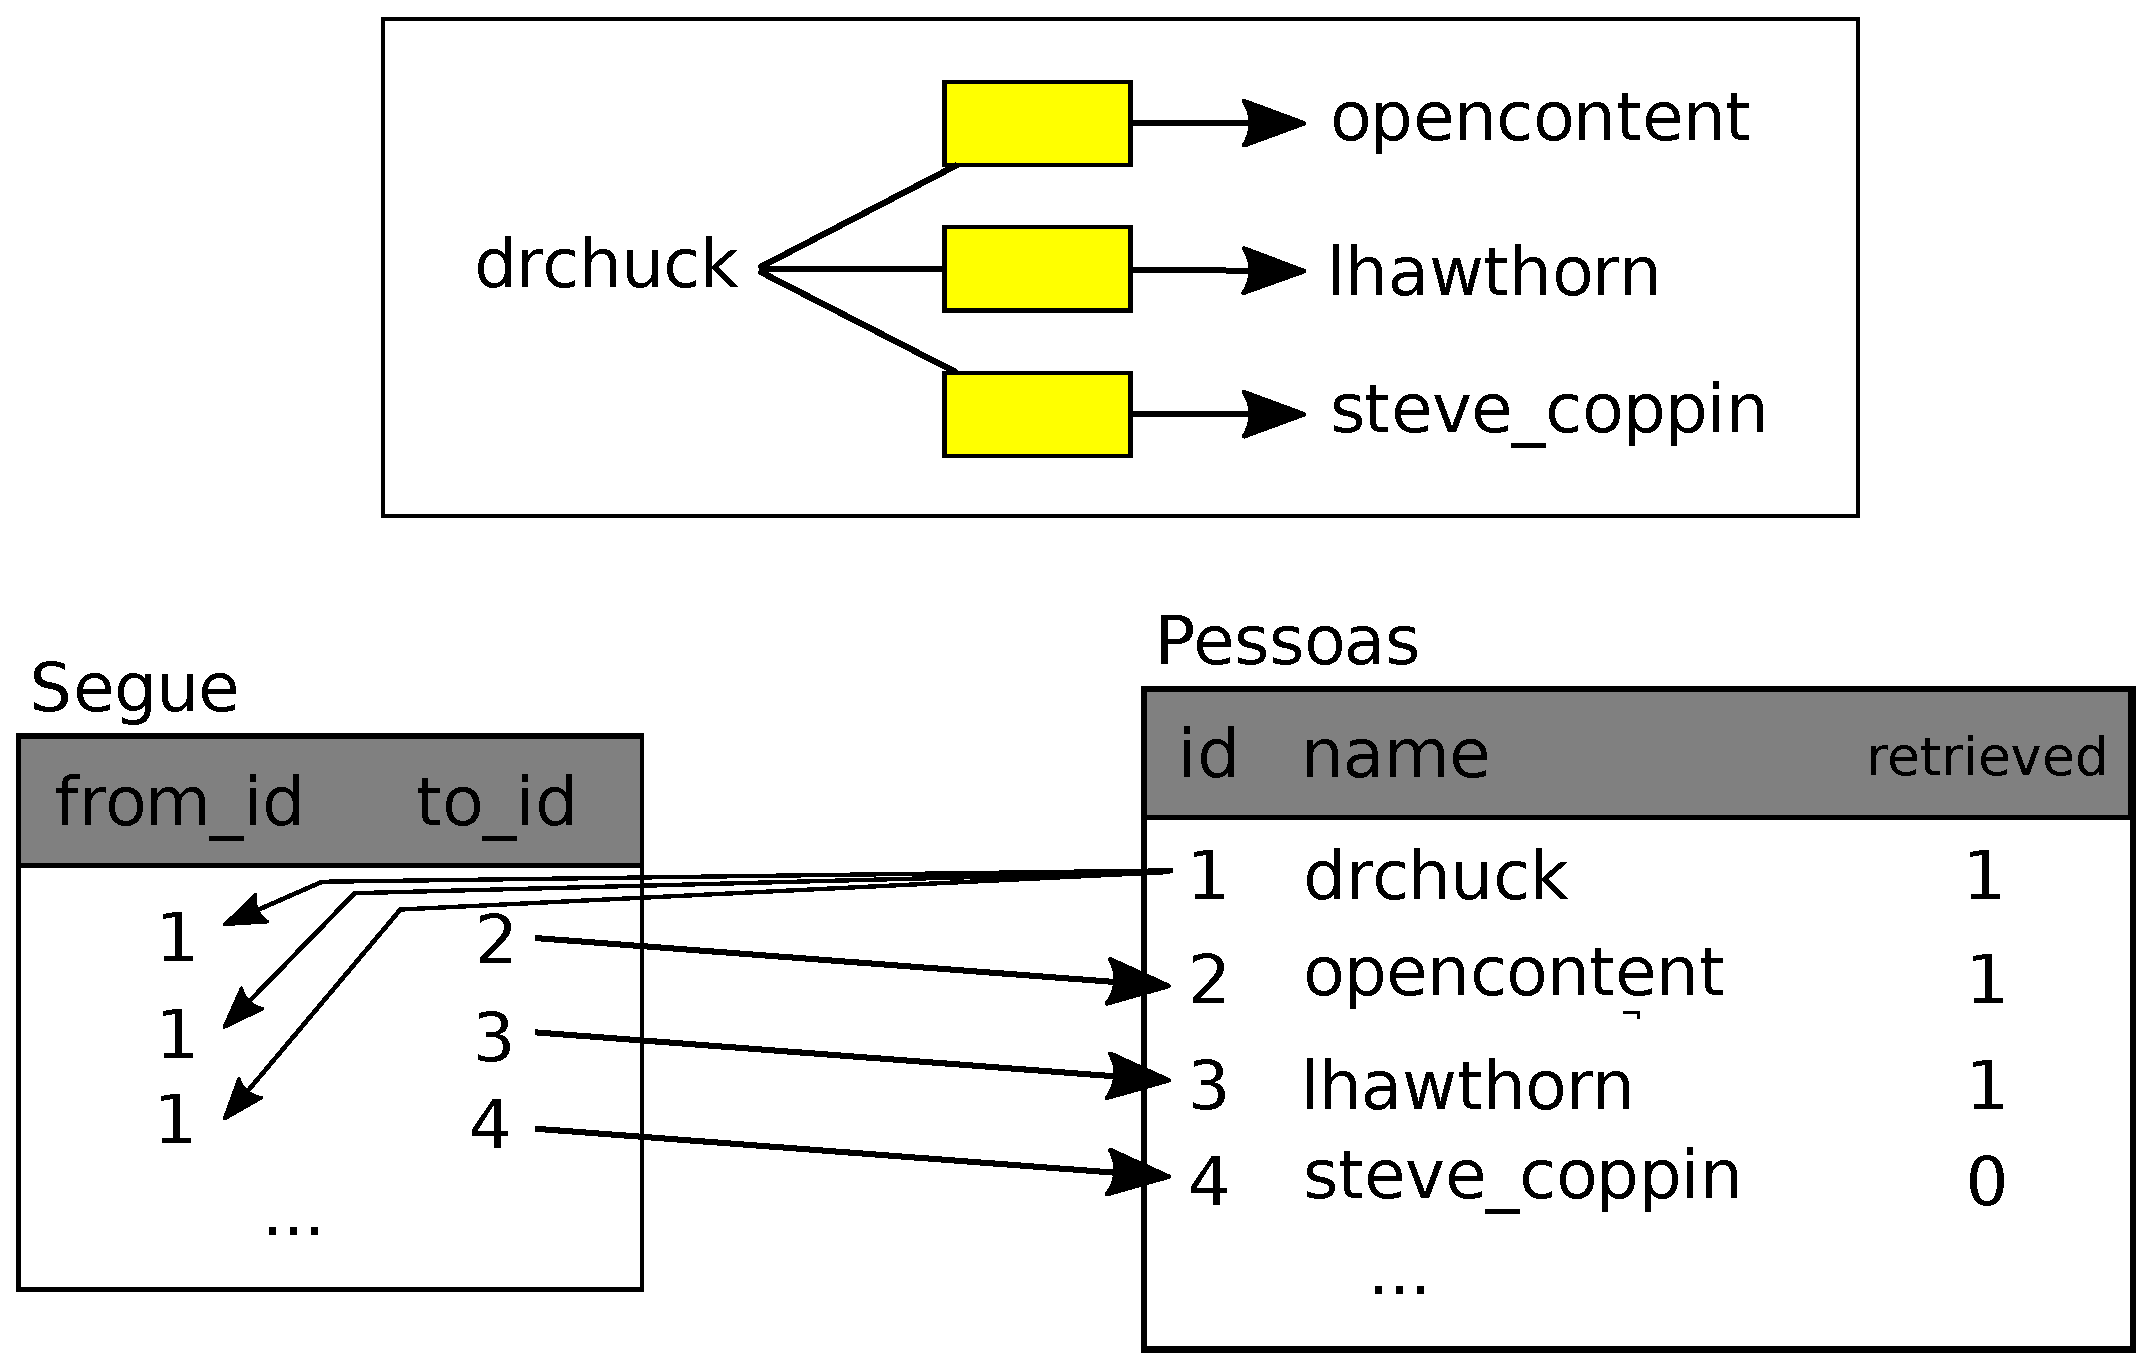
\includegraphics[height=2.50in]{figs2/twitter.eps}}
\afterfig


%\section{Programming with multiple tables}
\section{Programando com múltiplas tabelas}

%We will now redo the Twitter spider program using two tables, the primary
%keys, and the key references as described above.  Here is the code for 
%the new version of the program:

Agora nós iremos refazer o programa de rastreio do Twitter utilizando duas
tabelas, as chaves primárias, e as chaves de referências estão descritas
anteriormente. Abaixo está o código da nova versão do programa:

\beforeverb
\begin{verbatim}
import urllib
import twurl
import json
import sqlite3

TWITTER_URL = 'https://api.twitter.com/1.1/friends/list.json'

conn = sqlite3.connect('friends.sqlitesqlite3')
cur = conn.cursor()

cur.execute('''CREATE TABLE IF NOT EXISTS People 
    (id INTEGER PRIMARY KEY, name TEXT UNIQUE, retrieved INTEGER)''')
cur.execute('''CREATE TABLE IF NOT EXISTS Follows 
    (from_id INTEGER, to_id INTEGER, UNIQUE(from_id, to_id))''')

while True:
    acct = raw_input('Enter a Twitter account, or quit: ')
    if ( acct == 'quit' ) : break
    if ( len(acct) < 1 ) :
        cur.execute('''SELECT id, name FROM People 
            WHERE retrieved = 0 LIMIT 1''')
        try:
            (id, acct) = cur.fetchone()
        except:
            print 'No unretrieved Twitter accounts found'
            continue
    else:
        cur.execute('SELECT id FROM People WHERE name = ? LIMIT 1', 
            (acct, ) )
        try:
            id = cur.fetchone()[0]
        except:
            cur.execute('''INSERT OR IGNORE INTO People (name, retrieved) 
                VALUES ( ?, 0)''', ( acct, ) )
            conn.commit()
            if cur.rowcount != 1 : 
                print 'Error inserting account:',acct
                continue
            id = cur.lastrowid

    url = twurl.augment(TWITTER_URL, 
       {'screen_name': acct, 'count': '20'} )
    print 'Retrieving account', acct
    connection = urllib.urlopen(url)
    data = connection.read()
    headers = connection.info().dict
    print 'Remaining', headers['x-rate-limit-remaining']

    js = json.loads(data)
    # print json.dumps(js, indent=4)

    cur.execute('UPDATE People SET retrieved=1 WHERE name = ?', (acct, ) )

    countnew = 0
    countold = 0
    for u in js['users'] :
        friend = u['screen_name']
        print friend
        cur.execute('SELECT id FROM People WHERE name = ? LIMIT 1', 
            (friend, ) )
        try:
            friend_id = cur.fetchone()[0]
            countold = countold + 1
        except:
            cur.execute('''INSERT OR IGNORE INTO People (name, retrieved) 
                VALUES ( ?, 0)''', ( friend, ) )
            conn.commit()
            if cur.rowcount != 1 :
                print 'Error inserting account:',friend
                continue
            friend_id = cur.lastrowid
            countnew = countnew + 1
        cur.execute('''INSERT OR IGNORE INTO Follows (from_id, to_id) 
            VALUES (?, ?)''', (id, friend_id) )
    print 'New accounts=',countnew,' revisited=',countold
    conn.commit()

cur.close()
\end{verbatim}
\afterverb
%
%This program is starting to get a bit complicated, but it illustrates
%the patterns that we need to use when we are
%using integer keys to link tables. The basic patterns are:

%
Este programa está começando a ficar um pouco complicado, mas ilustra os
padrões que precisamos para utilizar quando estamos usando chaves inteiras
para conectar as tabelas. Os padrões básicos são:

\begin{enumerate}

%\item Create tables with primary keys and constraints.
\item Criar tabelas com chaves primárias e restrições.
%\item When we have a logical key for a person (i.e., account
%name) and we need the {\tt id} value for the person,
%depending on whether or not the person is already
%in the {\tt People} table we either need to: 
%(1) look up the person in the {\tt People} table and 
%retrieve the {\tt id} value for the person 
%or (2) add the person to the {\tt People} table and get the 
%{\tt id} value for the newly added row.
\item Quando temos uma chave lógica para uma pessoa (i.e., conta) e precisamos
  do valor de {\tt id} para a pessoa, dependendo se a pessoa já está na tabela
  {\tt People}  ou não, também precisaremos de: (1) olhar para a pessoa na
  tabela {\tt People} e recuperar o valor de {\tt id} da pessoa, ou (2)
  adicionar a pessoa na tabela {\tt People} e pegar o valor de {\tt id} para
  a nova linha recém adicionada.
  
%\item Insert the row that captures the ``follows'' relationship.

\item Inserir a linha que captura a relação com ``segue''.
  
\end{enumerate}

%We will cover each of these in turn.
Vamos tratar cada um dos ítens acima, em partes.

%\subsection{Constraints in database tables}
\subsection{Restrições em uma tabela}

As we design our table structures, we can tell the database system 
that we would like it to enforce a few rules on us.   These rules
help us from making mistakes and introducing incorrect data into 
out tables.   When we create our tables:
Assim como projetamos a estrutura da tabela, podemos informar ao banco de dados
que gostaríamos de reforçar algumas regras. Estas regras nos ajudam a não
cometer enganos e a não inserir dados incorretos nas nossas tabelas. Quando
criamos nossas tabelas:

\beforeverb
\begin{verbatim}
cur.execute('''CREATE TABLE IF NOT EXISTS People 
    (id INTEGER PRIMARY KEY, name TEXT UNIQUE, retrieved INTEGER)''')
cur.execute('''CREATE TABLE IF NOT EXISTS Follows 
    (from_id INTEGER, to_id INTEGER, UNIQUE(from_id, to_id))''')
\end{verbatim}
\afterverb
%
%We indicate that the {\tt name} column in the {\tt People} table must be
%{\tt UNIQUE}.   We also indicate that the combination of the two numbers
%in each row of the {\tt Follows} table must be unique.  These constraints
%keep us from making mistakes such as adding the same relationship more than
%once.
Indicamos que a coluna {\tt name} na tabela {\tt People} deve ser {\tt UNIQUE}.
Também indicaremos que a combinação dos dois números em cada linha da tabela
{\tt Follows} devem ser únicos. Estas restrições nos mantém longe da
possibilidade de cometer enganos como adicionar a mesma relação mais de uma vez.

%We can take advantage of these constraints in the following code:
Podemos obter vantagens destas restrições conforme mostra o seguinte código:

\beforeverb
\begin{verbatim}
cur.execute('''INSERT OR IGNORE INTO People (name, retrieved) 
    VALUES ( ?, 0)''', ( friend, ) )
\end{verbatim}
\afterverb
%
%We add the {\tt OR IGNORE} clause to our {\tt INSERT} statement to indicate
%that if this particular {\tt INSERT} would cause a violation of the
%``{\tt name} must be unique'' rule, the database system is allowed to ignore the 
%{\tt INSERT}.  We are using the database constraint as a safety net
%to make sure we don't inadvertently do something incorrect.
%
Adicionamos a condição {\tt OR IGNORE} a declaração {\tt INSERT} para indicar
que se este {\tt INSERT} em particular pode causar uma violação para a regra
``{\tt name} deve ser único'', assim o banco de dados tem permissão de ignorar
o {\tt INSERT}.

%Similarly, the following code ensures that we don't add the 
%exact same {\tt Follows} relationship twice.
De forma similar, o seguinte código garante que não adicionemos a mesma relação
{\tt Follows} duas vezes.

\beforeverb
\begin{verbatim}
cur.execute('''INSERT OR IGNORE INTO Follows 
    (from_id, to_id) VALUES (?, ?)''', (id, friend_id) )
\end{verbatim}
\afterverb
%
%Again, we simply tell the database to ignore our attempted 
%{\tt INSERT} if it would violate the uniqueness constraint
%that we specified for the {\tt Follows} rows.
Novamente, nós simplesmente dizemos para o banco de dados ignorar nossa
tentativa de inserir {\tt INSERT} se isto violar a regra de exclusividade que
especificamos para a linha {\tt Follows}.

%\subsection{Retrieve and/or insert a record}
\subsection{Restaurar e/ou inserir um registro}

%When we prompt the user for a Twitter account, if the account 
%exists, we must look up its {\tt id} value.  If the account
%does not yet exist in the {\tt People} table, we must insert 
%the record and get the {\tt id} value from the inserted
%row.

Quando solicitamos ao usuário uma conta do Twitter, se a conta existir,
precisamos verificar o valor do {\tt id}. Se a conta não existir ainda
na tabela {\tt People}, devemos inserir o registro e pegar o valor do
{\tt id} da linha inserida.

%This is a very common pattern and is done twice in the program above.
%This code shows how we look up the {\tt id} for a 
%friend's account when we have extracted a \verb"screen_name"
%from a {\tt user} node in the retrieved Twitter JSON.

Isto é um padrão muito comum e é feito duas vezes no programa acima. Este
código mostra como verificamos o {\tt id} da conta de um amigo, quando
extraímos um \verb"screen_name" de um nó de {\tt user} recuperado do JSON
do Twitter.

%Since over time it will be increasingly likely that the account
%will already be in the database, we first check to see if the
%{\tt People} record exists using a {\tt SELECT} statement.

Ao longo do tempo será cada vez mais provável que a conta já esteja registrada
no banco de dados, então primeiro checamos para ver se o registro existe em
{\tt People} utilizando uma declaração de {\tt SELECT}.

%If all goes well\footnote{In general, when a sentence starts 
%with ``if all goes well'' you will find that the code needs
%to use try/except.} inside the {\tt try} section, we retrieve the
%record using {\tt fetchone()} and then retrieve the
%first (and only) element of the returned tuple and store it in 
%\verb"friend_id".

Se tudo estiver certo\footnote{Em geral, quando uma sentença inicia com ``se
  tudo estiver certo'' você verá que o código precisa utilizar a condição
  {\it try/except}.} dentro da seção {\tt try}, recuperamos o registro usando
{\tt fetchone()} e depois recuperar o primeiro (e somente o primeiro) elemento
da tupla que retornou e a armazenamos em \verb"friend_id".

%If the {\tt SELECT} fails, the {\tt fetchone()[0]} code will fail
%and control will transfer into the {\tt except} section.

Se o {\tt SELECT} falhar, o código de {\tt fetchone()[0]} falhará e o controle
irá mudar para a seção {\tt except}.

\beforeverb
\begin{verbatim}
        friend = u['screen_name']
        cur.execute('SELECT id FROM People WHERE name = ? LIMIT 1',
            (friend, ) )
        try:
            friend_id = cur.fetchone()[0]
            countold = countold + 1
        except:
            cur.execute('''INSERT OR IGNORE INTO People (name, retrieved) 
                VALUES ( ?, 0)''', ( friend, ) )
            conn.commit()
            if cur.rowcount != 1 :
                print 'Error inserting account:',friend
                continue
            friend_id = cur.lastrowid
            countnew = countnew + 1
\end{verbatim}
\afterverb
%
%If we end up in the {\tt except} code, it simply means that the row
%was not found, so we must insert the row.  We use {\tt INSERT OR 
%IGNORE} just to avoid errors and then call {\tt commit()} to 
%force the database to really be updated.  After the write is done, we can 
%check the {\tt cur.rowcount} to see how many rows were affected.  Since
%we are attempting to insert a single row, if the number of 
%affected rows is something other than 1, it is an error.  

Se terminar no código do {\tt except}, isto significa que aquela linha não foi
encontrada, então devemos inserí-la na linha. Usamos o {\tt INSERT OR IGNORE}
somente para evitar erros e depois chamamos {\tt commit()} para forçar que a
base de dados seja atualizada. Depois que a escrita esteja completa, nós
podemos checar, com {\tt cur.rowcount}, para ver quantas linhas foram afetadas.
Uma vez que estamos tentando inserir uma simples linha, se o número de linhas
afetadas é alguma coisa diferente de 1, isto é um erro.

%If the {\tt INSERT} is successful, we can look at {\tt cur.lastrowid} 
%to find out what value the database assigned to the {\tt id} column in 
%our newly created row.

Se o {\tt INSERT} for executado com sucesso, nós podemos verificar, através do
{\tt cur.lastrowid} para descobrir qual valor o banco de dados associou na
coluna {\tt id} na nossa nova linha.

%\subsection{Storing the friend relationship}
\subsection{Armazenando a conexão do amigo}

%Once we know the key value for both the Twitter user
%and the friend in the JSON, it is a simple matter to insert
%the two numbers into the {\tt Follows} table
%with the following code:

Uma vez que sabemos o valor da chave para o usuário do Twitter e o amigo
extraído do JSON, simplesmente inserimos os dois números dentro da tabela
{\tt Follows} com o seguinte código:

\beforeverb
\begin{verbatim}
cur.execute('INSERT OR IGNORE INTO Follows (from_id, to_id) VALUES (?, ?)',
    (id, friend_id) )
\end{verbatim}
\afterverb
%
%Notice that we let the database take care of keeping us from ``double-inserting''
%a relationship by creating the table with a uniqueness constraint and then
%adding {\tt OR IGNORE} to our {\tt INSERT} statement.
%
Note que deixamos o banco de dados cuidar para nós de realizar a
``inserção-dupla'' da conexão criando a tabela com a restrição única e depois
adicionando {\tt OR IGNORE} a nossa condição de {\tt INSERT}.

%Here is a sample execution of this program:
Esta é um exemplo de execução deste programa:

\beforeverb
\begin{verbatim}
Enter a Twitter account, or quit: 
No unretrieved Twitter accounts found
Enter a Twitter account, or quit: drchuck
Retrieving http://api.twitter.com/1.1/friends ...
New accounts= 20  revisited= 0
Enter a Twitter account, or quit: 
Retrieving http://api.twitter.com/1.1/friends ...
New accounts= 17  revisited= 3
Enter a Twitter account, or quit: 
Retrieving http://api.twitter.com/1.1/friends ...
New accounts= 17  revisited= 3
Enter a Twitter account, or quit: quit
\end{verbatim}
\afterverb
%
%We started with the {\tt drchuck} account and then let the program
%automatically pick the next two accounts to retrieve and add to 
%our database.

%
Nós iniciamos com a conta {\tt drchuck} e depois deixamos o programa pegar
automaticamente as próximas duas contas para recuperar e adicionar a nossa
base de dados.

%The following is the first few rows in the {\tt People} 
%and {\tt Follows} tables after this run is completed:

Abaixo estão as primeiras linhas das tabelas {\tt People} e {\tt Follows}
depois que esta execução é finalizada:

\beforeverb
\begin{verbatim}
People:
(1, u'drchuck', 1)
(2, u'opencontent', 1)
(3, u'lhawthorn', 1)
(4, u'steve_coppin', 0)
(5, u'davidkocher', 0)
55 rows.
Follows:
(1, 2)
(1, 3)
(1, 4)
(1, 5)
(1, 6)
60 rows.
\end{verbatim}
\afterverb
%
%You can see the {\tt id}, {\tt name}, and {\tt visited} fields in the 
%{\tt People} table and you see the numbers of both ends of 
%the relationship in the {\tt Follows} table.   
%In the {\tt People} table, we can see that the first three people
%have been visited and their data has been retrieved.
%The data in the {\tt Follows} table indicates that
%{\tt drchuck} (user 1) is a friend to all of the people shown in the first
%five rows.  This makes sense because
%the first data we retrieved and stored was the Twitter friends of
%{\tt drchuck}.  If you were to print more rows from the {\tt Follows} table,
%you would see the friends of users 2 and 3 as well.

%
Você também pode ver os campos {\tt id}. {\tt name} e {\tt visited} na tabela
{\tt People} e os números dos finais das conexões na tabela {\tt Follows}. Na
tabela {\tt People}, podemos ver que as primeiras três pessoas foram visitadas
e seus dados foram recuperados. Os dados na tabela {\tt Follows} indica que
{\tt drchuck} (usuário 1) é amigo de todas as pessoas mostradas nas primeiras
cincos linhas. Isto mostra que o primeiro dado que recuperamos e armazenamos
foram dos amigos do {\tt drchuck}. Se você mostrou mais linhas da tabela
{\tt Follows}, você poderá ver os amigos dos usuários 2 e 3.

%\section{Three kinds of keys}
\section{Três tipos de chaves}

%Now that we have started building a data model putting our
%data into multiple linked tables and linking the rows in those
%tables using {\bf keys}, we need to look at some terminology 
%around keys.  There are generally three kinds of keys used 
%in a database model.

Agora que iniciamos a construção de um modelo de dados colocando nossos dados
dentro de múltiplas tabelas e linhas conectadas nestas tabelas utilizando
{\bf chaves}, precisamos olhar para algumas terminologias sobre as chaves.
Existem genericamentes três tipos de chaves que são utilizadas em um banco de
dados.

\begin{itemize}

%\item A {\bf logical key} is a key that the ``real world'' might use
%to look up a row.   In our example data model, the {\tt name}
%field is a logical key.  It is the screen name for the user 
%and we indeed look up a user's row several times in the program
%using the {\tt name} field.  You will often find that it makes
%sense to add a {\tt UNIQUE} constraint to a logical key.  Since the 
%logical key is how we look up a row from the outside world, it makes
%little sense to allow multiple rows with the same value in the table.

\item Um {\bf chave lógica} é uma chave que o ``mundo real'' pode usar para
  checar uma linha. Na nossa modelagem, o campo {\tt name} é uma chave lógica.
  Ele é o nome que usamos para o usuário e nós na verdade para uma linha de
  usuário diversas vezes no nosso programa usando o campo {\tt name}. Você
  perceberá que faz sentido adicionar a restrição de {\tt UNIQUE} para uma
  chave lógica. Uma vez que é através de chaves lógicas que consultamos uma
  linha do mundo exterior, faz um pouco de sentido permitir que múltiplas
  linhas tenham o mesmo valor em uma tabela.
  
%\item A {\bf primary key} is usually a number that is assigned
%automatically by the database.  It generally has no meaning outside
%the program and is only used to link rows from different tables
%together.  When we want to look up a row in a table, usually 
%searching for the row using the primary key is the fastest 
%way to find the row.  Since primary keys are integer numbers, they 
%take up very little storage and can be compared or sorted very quickly.
%In our data model, the {\tt id} field is an example of a primary key.

\item Um {\bf chave primária} é usualmente um número que é associado
  automaticamente por um banco de dados. Geralmente não terá significado fora
  do programa e só é utilizada para conectar as linhas de diferentes tabelas.
  Quando queremos verificar uma linha em uma tabela, normalmente buscamos pela
  linha utilizando a chave primária, é a forma mais rápida de encontrar uma
  linha. Uma vez que chaves primárias são números inteiros, eles ocupam pouco
  espaço e podem ser comparados ou ordenados rapidamente. No nosso modelo, o
  campo {\tt id} é um exemplo de chave primária.
  
%\item A {\bf foreign key} is usually a number that points to the primary key
%of an associated row in a different table.  An example of a foreign
%key in our data model is the \verb"from_id".  

\item Uma {\bf chave estrangeira} é normalmente um número que aponta para a
  chave primária associada a uma linha em outra tabela. Um exemplo de chave
  estrangeira no nosso modelo é o campo \verb"from_id".
\end{itemize}

%We are using a
%naming convention of always calling the primary key field name
%{\tt id} and appending the suffix \verb"_id" to any field name
%that is a foreign key.

Nós estamos utilizando uma convenção de sempre chamar uma chave primária de
um campo {\tt id} e adicionando o sufixo \verb"_id" para qualquer campo que
seja uma chave estrangeira.

%\section{Using JOIN to retrieve data}
\section{Utilizando o JOIN para recuperar informações}

%Now that we have followed the rules of database normalization
%and have data separated into two tables, linked together using
%primary and foreign keys, we need to be able to build a 
%{\tt SELECT} that reassembles the data across the tables.

Agora que seguimos as regras de normalização de bancos de dados e temos os
dados separados em duas tabelas, associadas através de chaves primárias e
chaves estrangeiras, precisamos ser capazes de construir uma chamada de
{\tt SELECT} que reagrupa os dados em toda as tabelas.

%SQL uses the {\tt JOIN} clause to reconnect these tables.  
%In the {\tt JOIN} clause you specify the fields that are used 
%to reconnect the rows between the tables.

SQL utiliza a cláusula {\tt JOIN} para reconectar estas tabelas. Na cláusula
{\tt JOIN} você especifica o campo que serão utilizados para reconectar as
linhas entre as tabelas.

%The following is an example of a {\tt SELECT} with a 
%{\tt JOIN} clause:

Abaixo, um exemplo de um {\tt SELECT} com um {\tt JOIN}:

\beforeverb
\begin{verbatim}
SELECT * FROM Follows JOIN People 
    ON Follows.from_id = People.id WHERE People.id = 1
\end{verbatim}
\afterverb
%
The {\tt JOIN} clause indicates that the fields we are selecting
cross both the {\tt Follows} and {\tt People} tables.  The {\tt ON}
clause indicates how the two tables are to be joined:  Take the rows
from {\tt Follows} and append the row from {\tt People} where the
field \verb"from_id" in {\tt Follows} is the same the {\tt id} value
in the {\tt People} table.

%
O {\tt JOIN} indica que o cmapo que utilizamos são selecionados cruzando ambas
as tabelas {\tt Follows} e {\tt People}. A cláusula {\tt ON} indica como as
duas tabelas devem ser unidas: Junta as linhas da tabela {\tt Follows} às da
tabela {\tt People} onde o campo \verb"from_id" em {\tt Follows} tem o mesmo
valor do campo {\tt id} na tabela {\tt People}.

\beforefig
\centerline{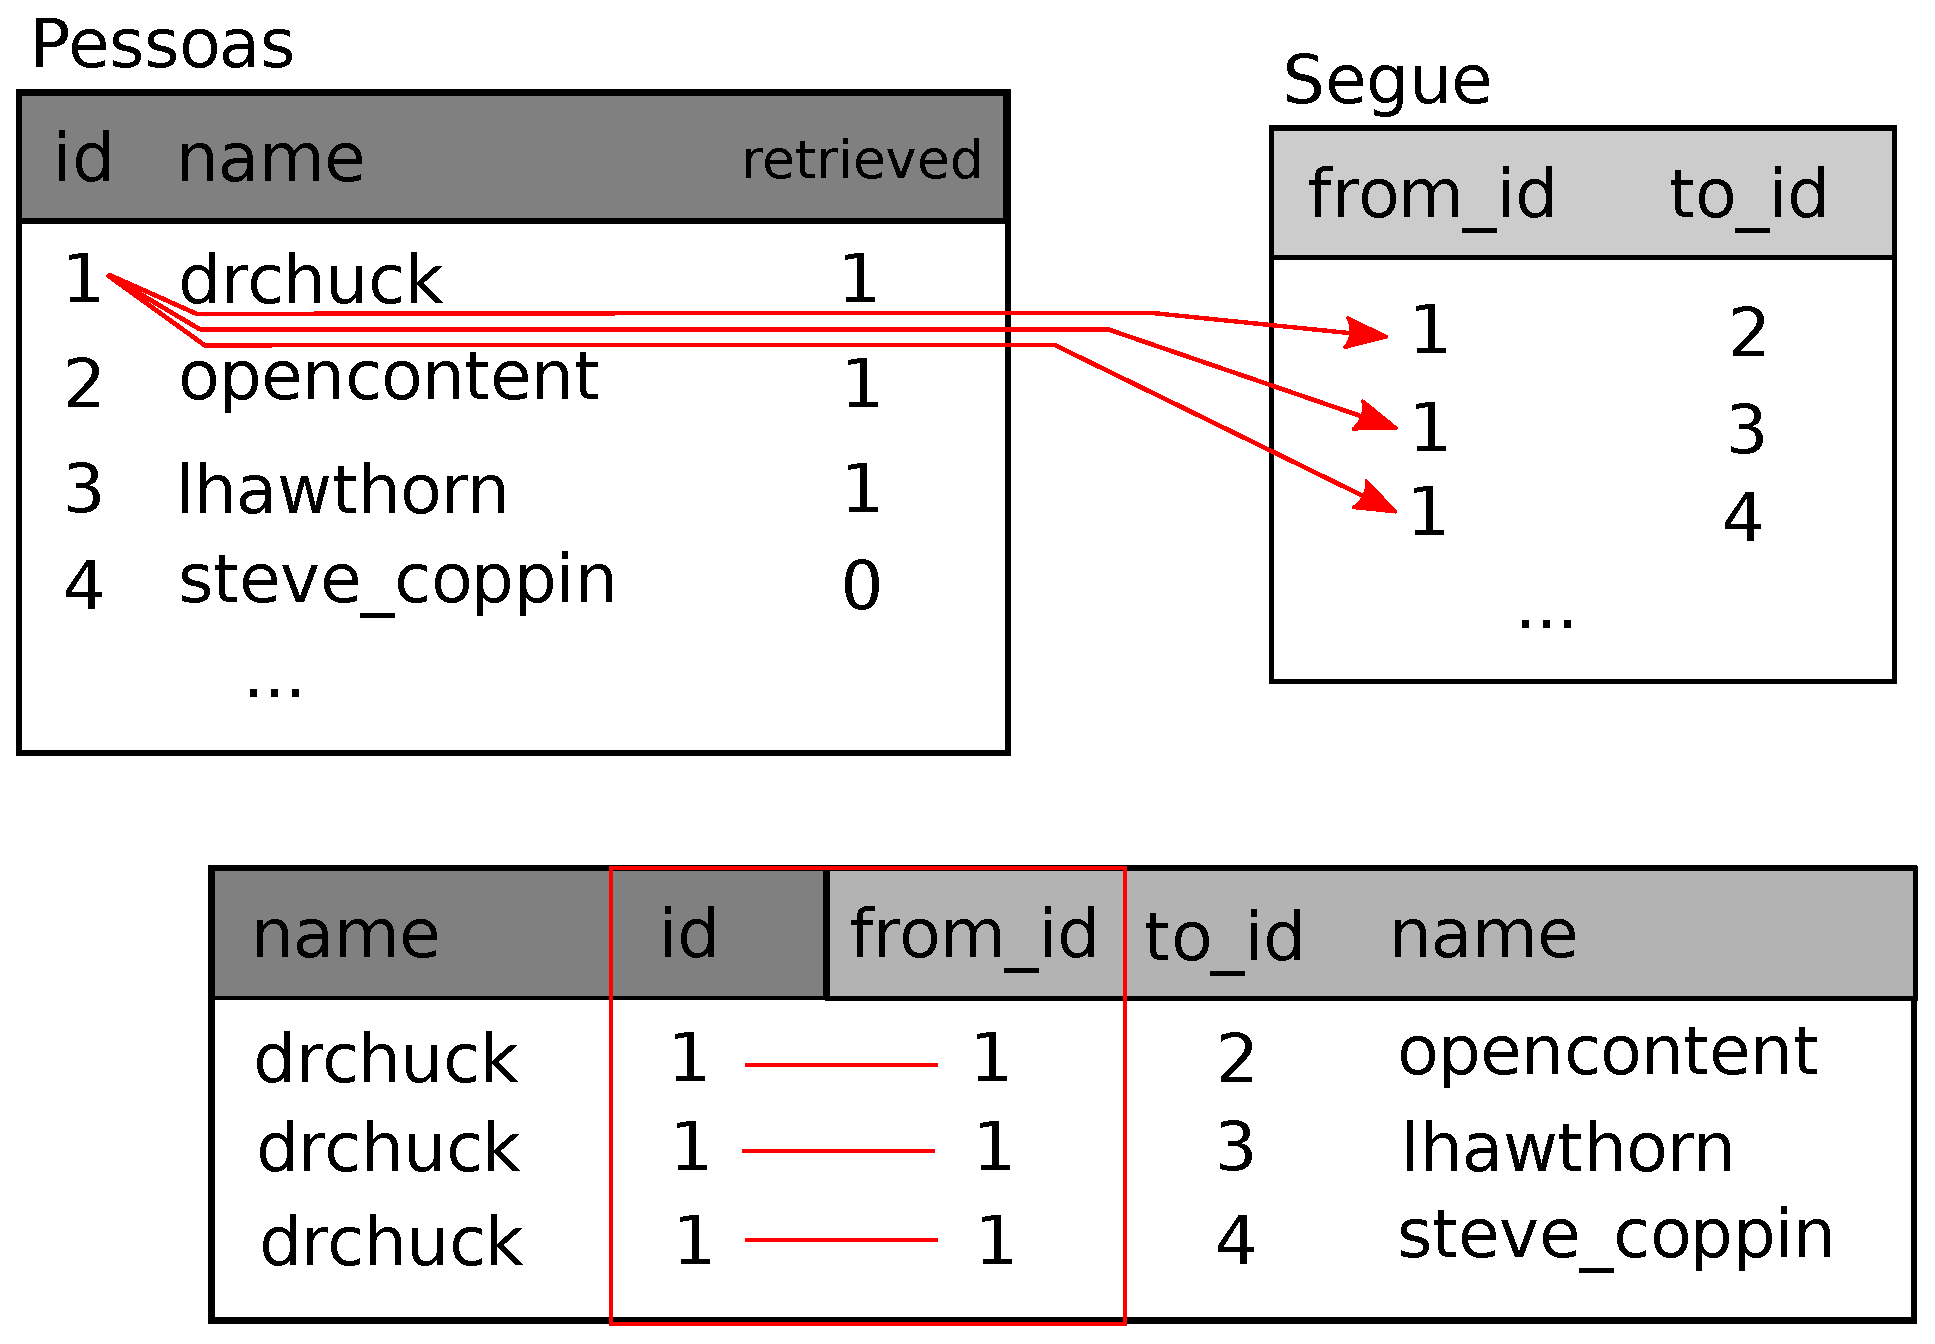
\includegraphics[height=2.50in]{figs2/join.eps}}
\afterfig

%The result of the JOIN is to create extra-long ``metarows'' which have both 
%the fields from {\tt People} and the matching fields from {\tt Follows}.
%Where there is more than one match between the {\tt id} field from {\tt People}
%and the \verb"from_id" from {\tt People}, then JOIN creates a metarow 
%for \emph{each} of the matching pairs of rows, duplicating data as needed.

O resultado do {\tt JOIN} cria uma super ``metalinha'' que tem os dois campos
da tabela {\tt People} que casam com os campos da tabela {\tt Follows}. Onde
existir mais de uma ocorrência entre o campo {\tt id} e o \verb"from_id" da
tabela {\tt People}, então o {\tt JOIN} cria uma ``metalinha'' para \emph{cada}
par de linhas que correspondem, duplicando os dados conforme for necessário.

%The following code demonstrates the data that we will have in the 
%database after the multi-table Twitter spider program (above) has
%been run several times.

O seguinte código demonstra o dado que nós teremos no banco de dados após o
executar o programa coletor de dados (acima) diversas vezes.

\beforeverb
\begin{verbatim}
import sqlite3

conn = sqlite3.connect('spider.sqlite3')
cur = conn.cursor()

cur.execute('SELECT * FROM People')
count = 0
print 'People:'
for row in cur :
   if count < 5: print row
   count = count + 1
print count, 'rows.'

cur.execute('SELECT * FROM Follows')
count = 0
print 'Follows:'
for row in cur :
   if count < 5: print row
   count = count + 1
print count, 'rows.'

cur.execute('''SELECT * FROM Follows JOIN People 
    ON Follows.to_id = People.id WHERE Follows.from_id = 2''')
count = 0
print 'Connections for id=2:'
for row in cur :
   if count < 5: print row
   count = count + 1
print count, 'rows.'

cur.close()
\end{verbatim}
\afterverb
%
%In this program, we first dump out the {\tt People}
%and {\tt Follows} and then dump out a subset of the
%data in the tables joined together.

%
Neste programa, primeiro descarregamos a tabela {\tt People} e {\tt Follows} e
depois descarregamos um subconjunto de dados das tabelas juntos.

%Here is the output of the program:

Aqui temos a saída do programa:

\beforeverb
\begin{verbatim}
python twjoin.py 
People:
(1, u'drchuck', 1)
(2, u'opencontent', 1)
(3, u'lhawthorn', 1)
(4, u'steve_coppin', 0)
(5, u'davidkocher', 0)
55 rows.
Follows:
(1, 2)
(1, 3)
(1, 4)
(1, 5)
(1, 6)
60 rows.
Connections for id=2:
(2, 1, 1, u'drchuck', 1)
(2, 28, 28, u'cnxorg', 0)
(2, 30, 30, u'kthanos', 0)
(2, 102, 102, u'SomethingGirl', 0)
(2, 103, 103, u'ja_Pac', 0)
20 rows.
\end{verbatim}
\afterverb
%
%You see the columns from the {\tt People} and {\tt Follows} tables and the last
%set of rows is the result of the {\tt SELECT} with the {\tt JOIN} clause.

%
Você vê as colunas das tabelas {\tt People} e {\tt Follows} e por último
conjunto de linhas é o resultado do {\tt SELECT} com o {\tt JOIN}.

%In the last select, we are looking for accounts that are friends of 
%``opencontent'' (i.e., {\tt People.id=2}).

No último {\tt SELECT}, nós estamos procurando por contas que tem amigos de
``conteúdo aberto'' (i.e., {\tt People.id=2}).

%In each of the ``metarows'' in the last select, the first two columns are
%from the {\tt Follows}
%table followed by columns three through five from the {\tt People} table.  You can also
%see that the second column (\verb"Follows.to_id") matches the third column
%({\tt People.id}) in each of the joined-up ``metarows''.


Em cada uma das ``meta-linhas'' da última seleção, as primeiras duas colunas
são da tabela {\tt Follows} seguidas pelas colunas três até cinco da tabela
{\tt People}. Você também pode ver que a segunda coluna (\verb"Follows.to_id")
relaciona a terceira coluna ({\tt People.id}) em cada uma das ``meta-linha''
que foram juntas.

%\section{Summary}
\section{Sumário}

%This chapter has covered a lot of ground to give you an overview of the basics
%of using a database in Python.   It is more complicated to write the code to use 
%a database to store data than Python dictionaries or flat files so there is 
%little reason to use a database unless your application truly needs the capabilities
%of a database.  The situations where a database can be quite useful are: 
%(1) when your application needs to make small many random updates within a large data set,
%(2) when your data is so large it cannot fit in a dictionary and you need to 
%look up information repeatedly, or (3) when you have a long-running process that you
%want to be able to stop and restart and retain the data from one run to the next.

Este capítulo cobriu os fundamentos para o uso, básico, de banco de dados no
Python. É muito mais complicado escrever código para usar um banco de dados
para armazenar informações do que dicionários ou arquivos com Python, então
se existe poucas razões para utilizar um banco de dados, a menos que sua
aplicação realmente precise das capacidades de um banco de dados. As situações
onde um banco de dados podem ser muito úteis são: (1) quando sua aplicação
precisa realizar pequenas atualizações com um conjunto grande de dados, (2)
quando seus dados são tão grandes que não podem ser armazenados em um
dicionário e você precisa acessar estas informações repetidas vezes, ou (3)
quando você tem um processo de execução demorada e você quer ser capaz de
parar e recomeçar e manter os dados entre as pesquisas.

%You can build a simple database with a single table to suit many application 
%needs, but most problems will require several tables and links/relationships
%between rows in different tables.   When you start making links between 
%tables, it is important to do some thoughtful design and follow the 
%rules of database normalization to make the best use of the database's
%capabilities.  Since the primary motivation for using a database
%is that you have a large amount of data to deal with, it is important
%to model your data efficiently so your programs run as fast as possible.

Você pode construir um banco de dados simples com uma única tabela para
atender muitas aplicações, mas a maiorias dos problemas vão necessitar de
várias tabelas e conexões/relações entre as linhas em diferentes tabelas.
Quando você começar a fazer relações entre as tabelas, é importante fazer
algum planejamento e seguir as regras de normatização de banco de dados
para fazer um melhor uso das capacidades dos bancos de dados. Uma vez que a
principal motivação para utilizar um banco de dados é que você tem um grande
conjunto de dados para tratar, é importante modelar os dados eficientemente,
assim seus programas poderão rodas tão rápido quanto for possível.

%\section{Debugging}
\section{Depuração}
%One common pattern when you are developing a Python program to connect to
%an SQLite database will be to run a Python program and check the
%results using the SQLite Database Browser.  The browser allows you 
%to quickly check to see if your program is working properly.

É comum quando você está desenvolvendo um programa em Python para se conectar
em um banco de dados SQLite, é executar um programa para checar os resultados
utilizando o Navegador SQLite. O navegador permitirá que rapidamente verifique
se o seu programa está funcionando corretamente.

%You must be careful because SQLite takes care to keep two programs
%from changing the same data at the same time.   For example, if
%you open a database in the browser and make a change to the database
%and have not yet pressed the ``save'' button in the browser, the 
%browser ``locks'' the database file and keeps any other program
%from accessing the file.  In particular, your Python program
%will not be able to access the file if it is locked.

Você deve ter cuidado, porque o SQLite cuida para que dois programas não
façam modificações nos dados ao mesmo tempo. Por exemplo, se você abrir
um banco de dados no navegador e faz alterações no banco de dados, enquanto
não pressionar o botão ``salvar'', o navegador ``trava'' o arquivo do banco
de dados e impede qualquer outro programa de acessar o arquivo. Desta forma
seu programa em Python não conseguirá acessar o arquivo se ele estiver travado.

%So a solution is to make sure to either close the database browser 
%or use the {\bf File} menu to close the database in the browser
%before you attempt to access the database from Python to avoid
%the problem of your Python code failing because the database is
%locked.

Então, uma solução é garantir que fechou o navegador ou utilizar o menu
{\bf Arquivo} para fechar o banco de dados no navegador antes de tentar
acessar o banco de dados através do Python, evitando problemas no seu código
porque o banco de dados está travado.

%\section{Glossary}
\section{Glossário}

\begin{description}


%\item[attribute:] One of the values within a tuple.  More commonly
%called a ``column'' or ``field''.
%\index{attribute}

\item[atributo:] Um dos valores dentro de uma tupla. Comumente chamado de
  ``coluna'' ou ``campo''.
  \index{atributo}
  
%\item[constraint:] 
%When we tell the database to enforce a rule on a field or a row
%in a table.  A common constraint is to insist that there can be no
%duplicate values in a particular field (i.e., all the values must be unique).
  %\index{constraint}
  
\item[restrição:] Quando ordenamos a um banco de dados para reforçar uma regra
em um campo ou em uma linha na tabela. Uma restrição comum é insistir que não
pode haver valore duplicados em um campo em particular (i.e., todos os
valores tem que ser únicos).
\index{restrição}


%\item[cursor:] A cursor allows you to execute SQL commands in a database
%and retrieve data from the database.  A cursor is similar to 
%a socket or file handle for network connections and files, respectively.
%\index{cursor}

\item[cursor:] Um cursor permite execução de um comando SQL em um banco de
  dados e recuperar informações de um banco de dados. Um cursor é similar a
  um {\it socket} ou identificador de arquivos para uma conexão de rede e
  arquivos, respectivamente.
  \index{cursor}
  
%\item[database browser:] 
%A piece of software that allows you to directly connect to a database 
%and manipulate the database directly without writing a program.
%\index{database browser}

\item[navegador de banco de dados:] um conjunto de {\it software} que permite
  se conectar diretamente a um banco de dados e manipulá-lo diretamente, sem
  escrever um programa.
  \index{navegador de banco de dados}
  
%\item[foreign key:] A numeric key that points to the primary key of 
%a row in another table.  Foreign keys establish relationships between rows
%stored in different tables.
%\index{foreign key}

\item[chave estrangeira:] Uma chave numérica que aponta para uma chave primária
  de uma linha em outra tabela. Chaves estrangeiras estabelecem relações entre
  linhas armazenadas em diferentes tabelas.
  \index{chave estrangeira}
  
%\item[index:] Additional data that the database software maintains as rows
%and inserts into a table to make lookups very fast.
%\index{index}

\item[índice:] Dados adicionais que um banco de dados mantém, como linhas e
  inserções dentro de uma tabela para realizar consultas mais rápido.
  \index{índice}
  
%\item[logical key:] A key that the ``outside world'' uses to look up a particular
%row.  For example in a table of user accounts, a person's email address
%might be a good candidate as the logical key for the user's data. 
%\index{logical key}

\item[chave lógica:] Uma chave que o ``mundo externo'' utiliza para consultar
  uma linha em particular. Por exemplo em uma tabela de contas de usuários, o
  email de uma pessoa pode ser um bom candidato a chave lógica para a
  informação de usuário.
  \index{chave lógica}
  
%\item[normalization:] Designing a data model so that no data
%is replicated.  We store each item of data at one place in the database
%and reference it elsewhere using a foreign key.
%\index{normalization}
%\index{database normalization}

\item[normatização:] Projetar um modelo de dados para que nenhum dado seja
  replicado. Armazenamos cada item de dados em um lugar no banco de dados
  e referenciamos isso em qualquer lugar utilizando chave estrangeira.
  \index{normatização}
  \index{normatização de banco de dados}
  
%\item[primary key:] A numeric key assigned to each row that is used to 
%refer to one row in a table from another table.  Often the database
%is configured to automatically assign primary keys as rows are inserted.
%\index{primary key}

\item[chave primária:] Uma chave numérica associada a cada linha que é usada
  para referenciar uma linha em uma tabela de outra tabela. Normalmente o
  banco de dados é configurado para automaticamente associar chaves primárias
  assim que linhas são inseridas.
  \index{chave primária}
  
%\item[relation:] An area within a database that contains tuples and 
%attributes.  More typically called a ``table''.
%\index{relation}

\item[relação:] Uma área dentro do banco de dados que contém tuplas e
  atributos. Tipicamente chamada de ``tabela''.
  \index{relação}
  
%\item[tuple:] A single entry in a database table that is a set 
%of attributes.  More typically called ``row''.
%\index{tuple}

\item[tupla:] Uma entrada em um banco de dados que é um conjunto de atributos.
  Tipicamente chamado de ``linha''.
  \index{tupla}
\end{description}


% TODO % The contents of this file is 
% Copyright (c) 2009-  Charles R. Severance, All Righs Reserved

\chapter{Visualizando dados}
%\chapter{Visualizing data}

Até agora, nós aprendemos a linguagem Python, como utilizá-la,
para trabalhar com redes e banco de dados para manipular dados.
%So far we have been learning the Python language and then 
%learning how to use Python, the network, and databases 
%to manipulate data.

Neste capítulo, serão apresentadas três aplicações completas
que utilizarão todos estes conceitos para gerenciar e visualizar
dados. Você pode utilizar estas aplicações como exemplo de código
que podem ajudar na solução de problemas reais. 
%In this chapter, we take a look at three 
%complete applications that bring all of these things together
%to manage and visualize data.  You  might use these applications 
%as sample code to help get you started in solving a
%real-world problem.

Cada uma das aplicações é um arquivo ZIP que você pode fazer
download, extrair para o seu computador e executar.
%Each of the applications is a ZIP file that you can download
%and extract onto your computer and execute.

\section{Construindo um mapa no Google a partir de dados geocodificados}
\index{Google!map}
\index{Visualização!mapas}
%\section{Building a Google map from geocoded data}
%\index{Google!map}
%\index{Visualization!map}

Neste projeto, nós utilizaremos a API de geocodificação do
Google para obter algumas localizações geográficas informadas
pelos usuários de nomes de universidades e colocar os dados
em um mapa no Google.
%In this project, we are using the Google geocoding API
%to clean up some user-entered geographic locations of 
%university names and then placing the data on a Google
%map.  

\beforefig
\centerline{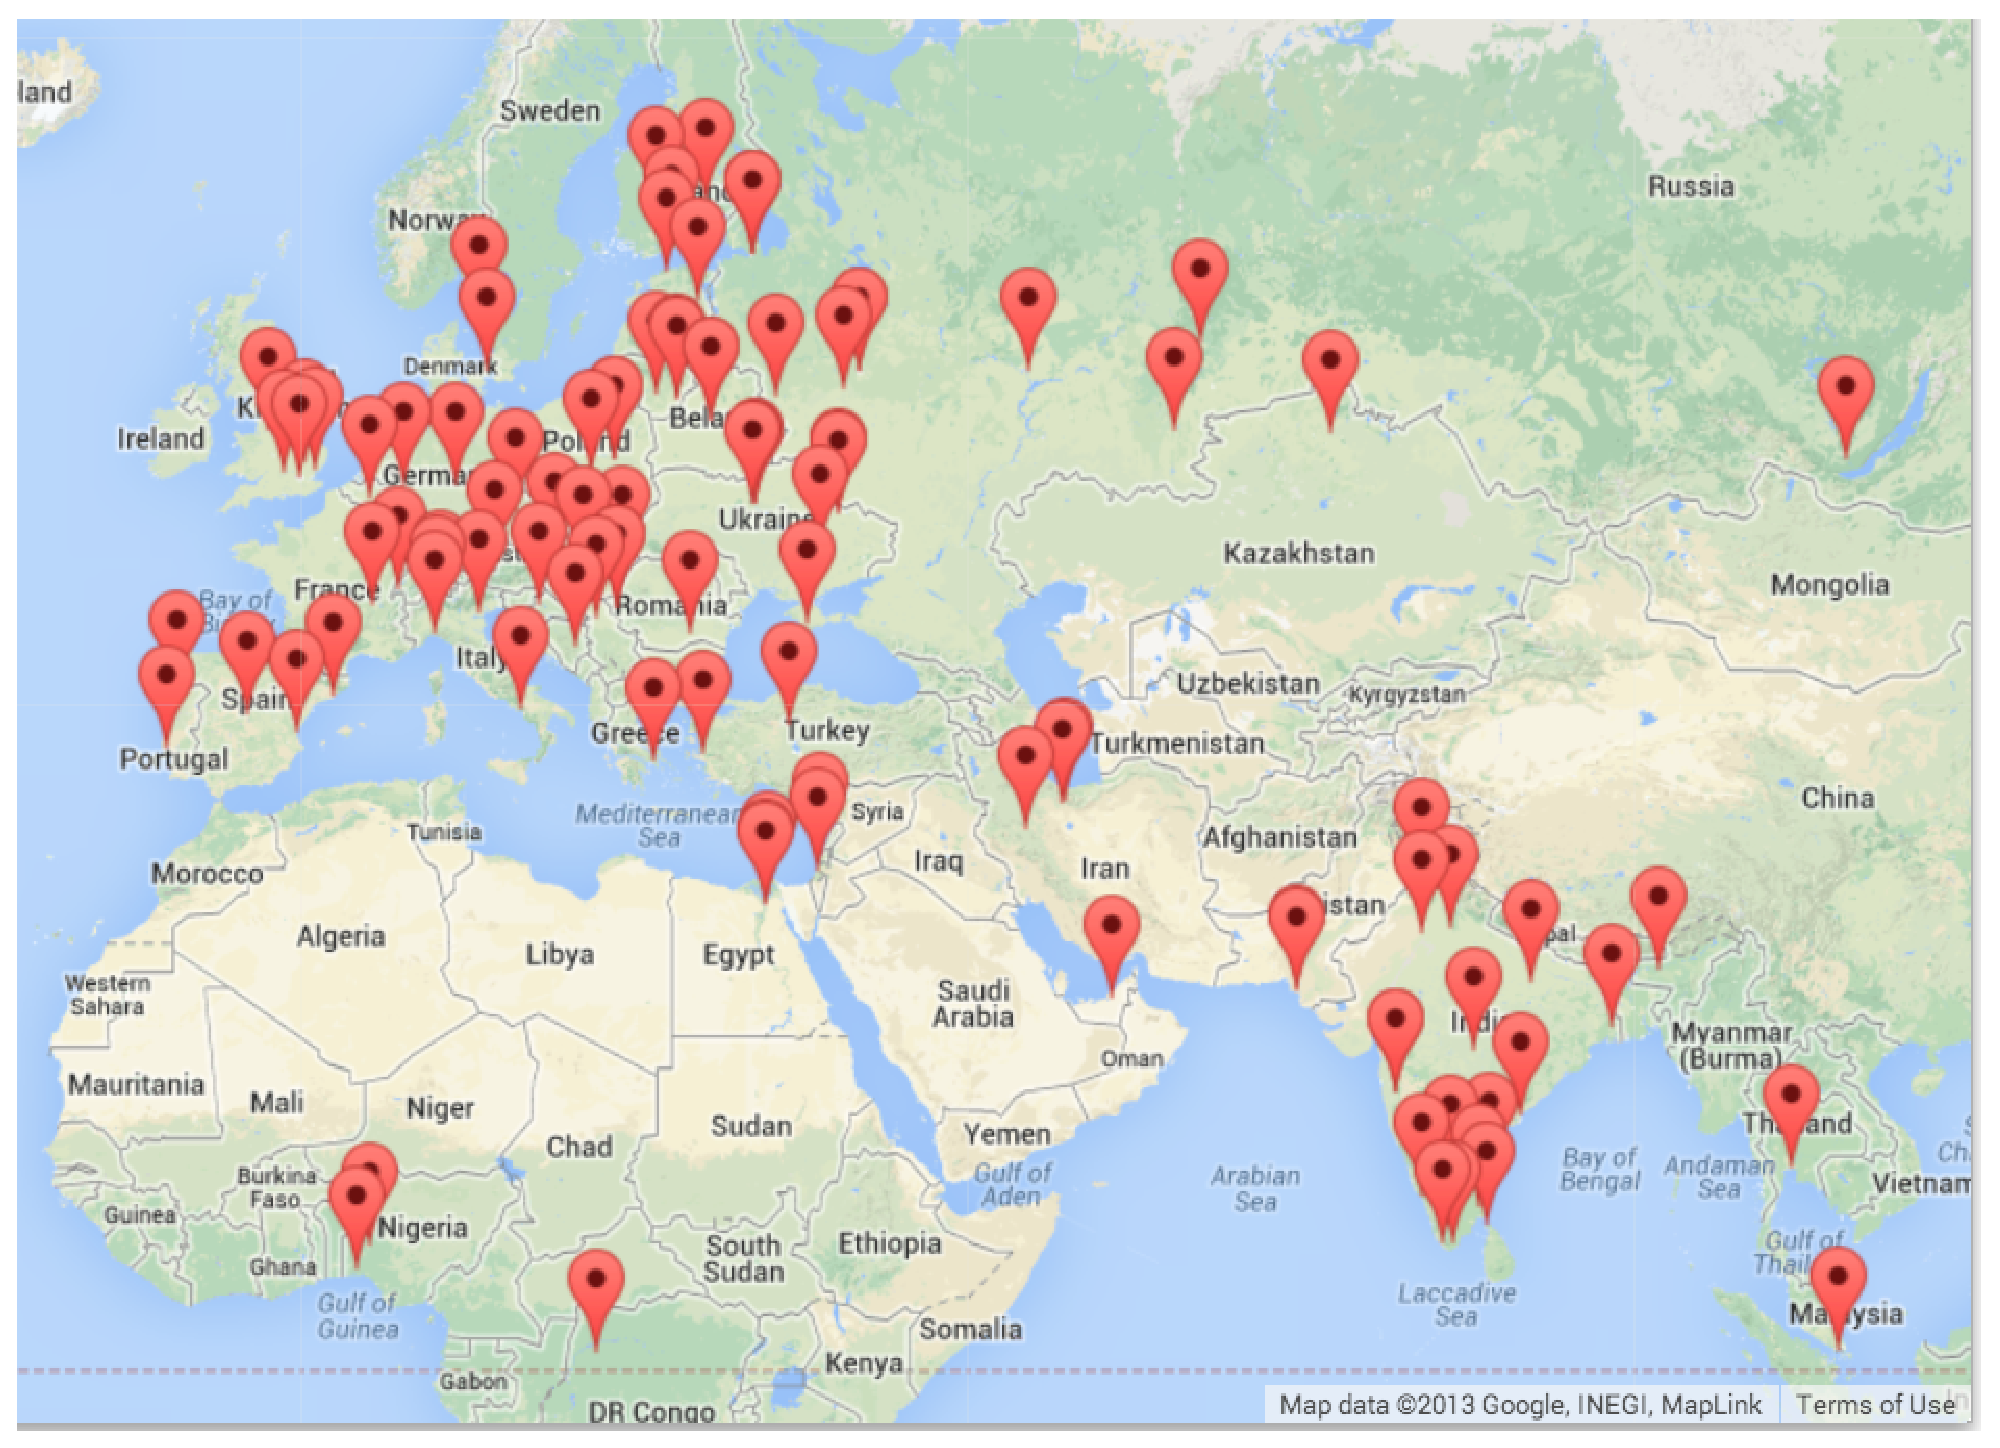
\includegraphics[height=2.25in]{figs2/google-map.eps}}
\afterfig
%\beforefig
%\centerline{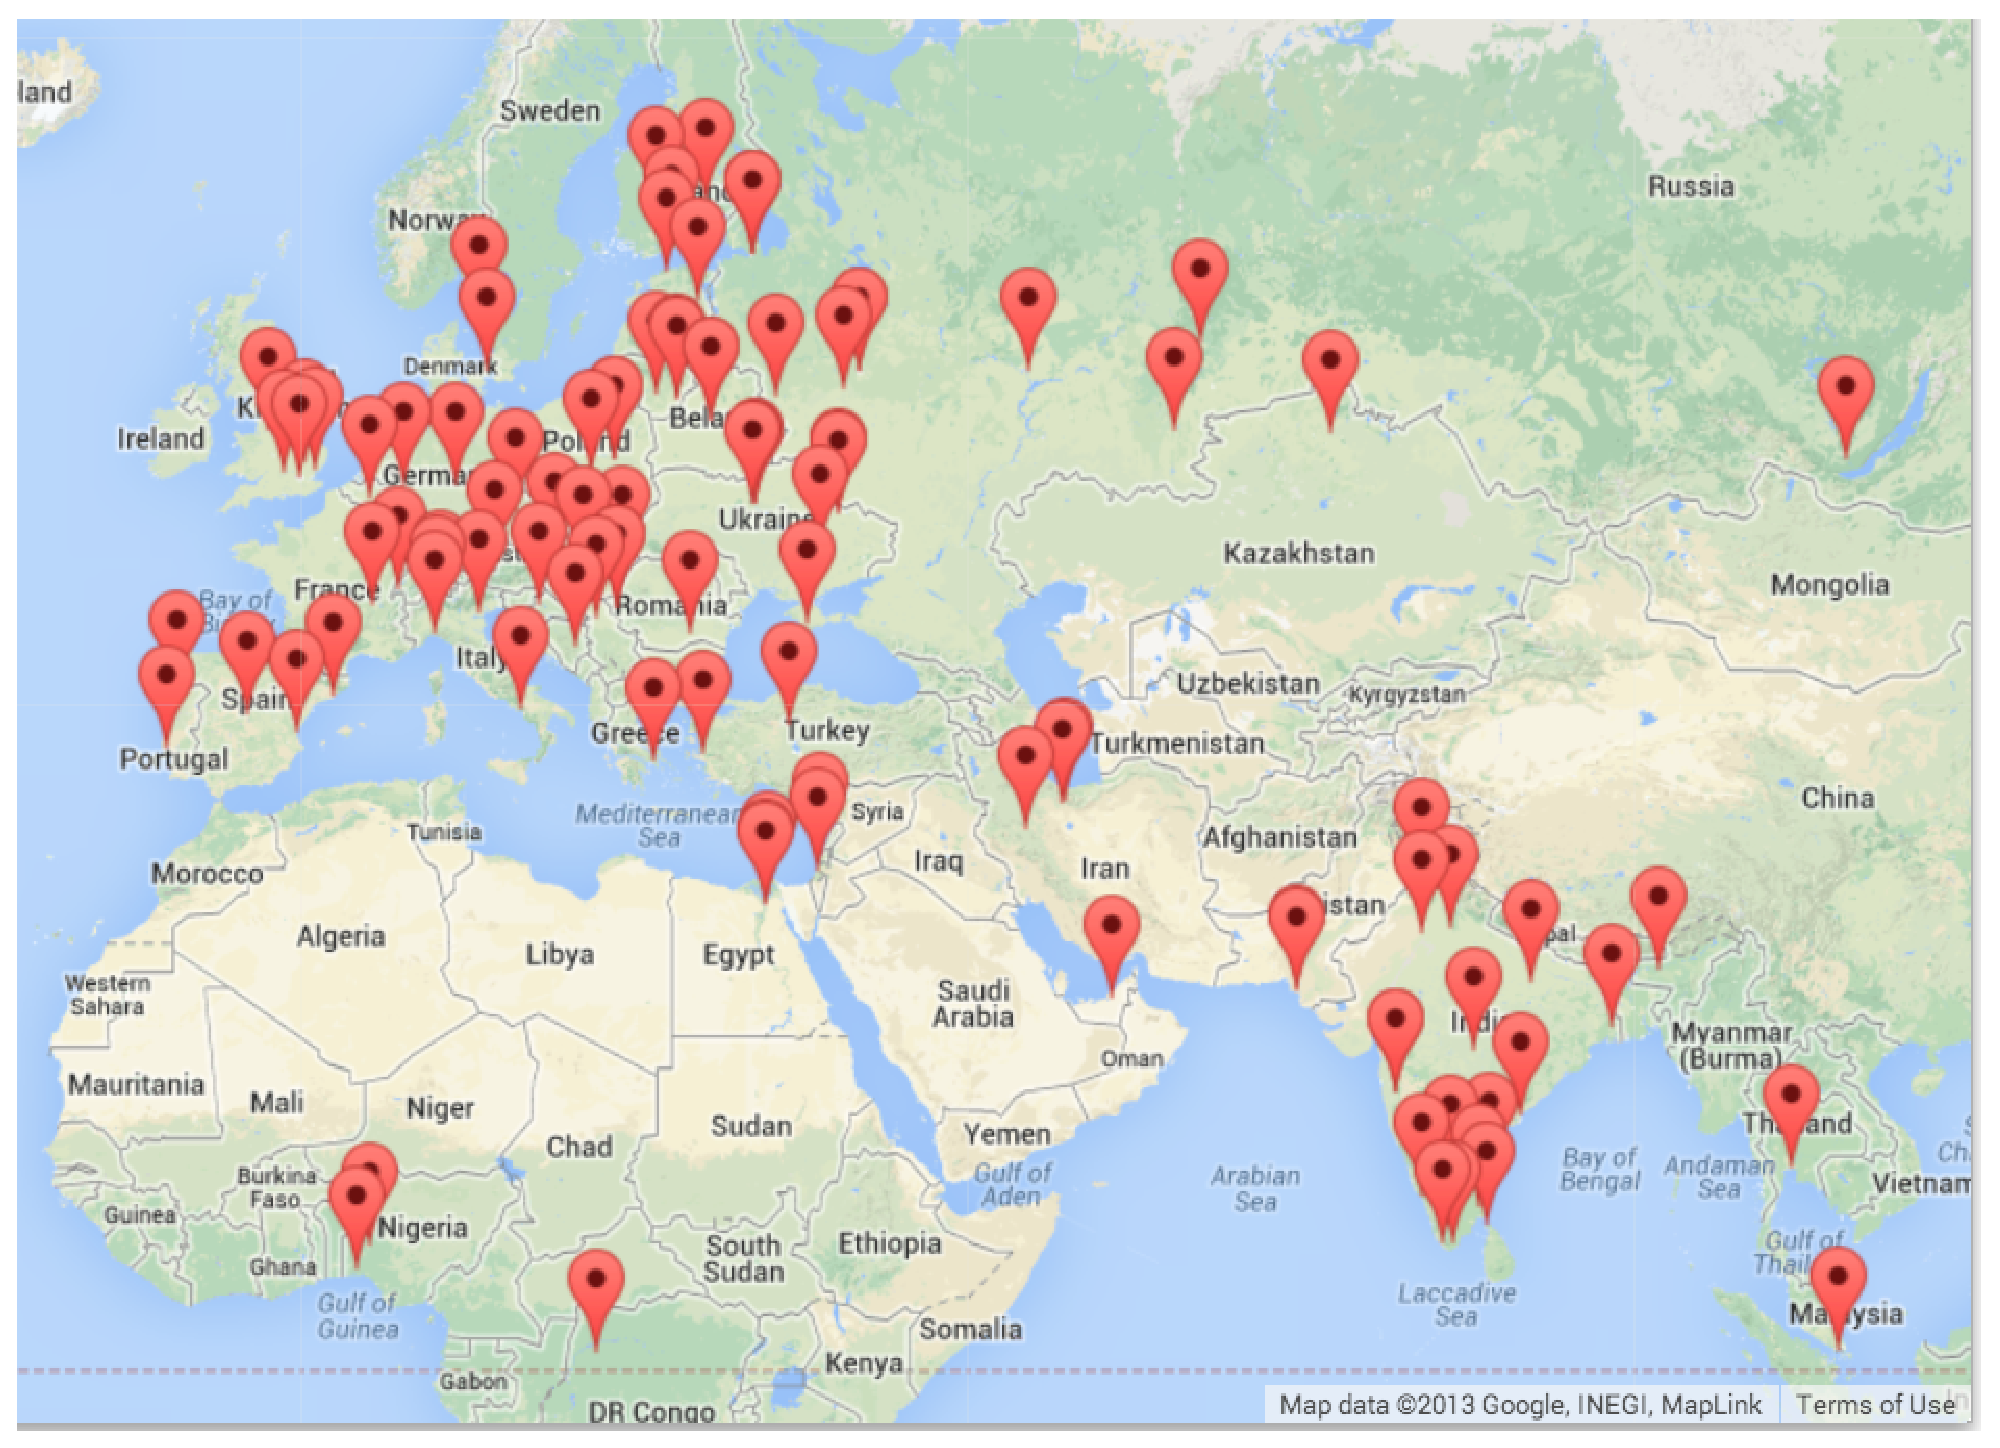
\includegraphics[height=2.25in]{figs2/google-map.eps}}
%\afterfig

Para iniciar, faça o download da aplicação em:
%To get started, download the application from:

\url{www.py4inf.com/code/geodata.zip}

O primeiro problema a ser resolvido é que a API gratuita de 
geocodificação do Google limita o número de requisições por dia.
Se você tiver muitos dados, você pode precisar parar e reiniciar
o processo de busca muitas vezes. Nós podemos quebrar o problema
em duas fases.
%The first problem to solve is that the free Google geocoding
%API is rate-limited to a certain number of requests per day.  If you have
%a lot of data, you might need to stop and restart the lookup
%process several times.  So we break the problem into two
%phases.  

\index{cache}
Na primeira fase nós faremos uma ``'pesquisa'' nos dados do arquivo
{\bf where.data} e então ler uma linha por vez, retornando a informação
geocodificada do Google e armazenar em um banco de dados {\bf geodata.sqlite}.
Antes de efetuar a pesquisa no Google, utilizando a API, para cada localização
informada pelo usuário, nós vamos checar para ver se já existe este dado
para a localização informada. O banco de dados está funcionando como um
``cache'' local dos nossos dados de localização para ter certeza que nunca
buscaremos no Google duas vezes pelo mesmo dado.
%\index{cache}
%In the first phase we take our input ``survey'' data in the file
%{\bf where.data} and read it one line at a time, and retrieve the
%geocoded information from Google and store it 
%in a database {\bf geodata.sqlite}.
%Before we use the geocoding API for each user-entered location, 
%we simply check to see if we already have the data for that 
%particular line of input.  The database is functioning as a 
%local ``cache'' of our geocoding data to make sure we never ask 
%Google for the same data twice.

Você pode reiniciar o processo a qualquer hora deletando o arquivo 
{\bf geodata.sqlite}.
%You can restart the process at any time by removing the file
%{\bf geodata.sqlite}.

Execute o programa {\bf geoload.py}. Este programa fará a leitura das linhas
do arquivo {\bf where.data} e para cada linha checar se o dado já existe no
banco de dados. Se nós não tivermos o dado para a localização, será utilizada
a API para retornar o dado e armazená-lo no banco de dados.  
%Run the {\bf geoload.py} program.   This program will read the input
%lines in {\bf where.data} and for each line check to see if it is already
%in the database.  If we don't have the data for the location, it will
%call the geocoding API to retrieve the data and store it in 
%the database.

Aqui está uma simples execução após a coleta de alguns dados no
banco de dados:
%Here is a sample run after there is already some data in the 
%database:

\beforeverb
\begin{verbatim}
Found in database  Northeastern University
Found in database  University of Hong Kong, ...
Found in database  Technion
Found in database  Viswakarma Institute, Pune, India
Found in database  UMD
Found in database  Tufts University

Resolving Monash University
Retrieving http://maps.googleapis.com/maps/api/
    geocode/json?sensor=false&address=Monash+University
Retrieved 2063 characters {    "results" : [  
{u'status': u'OK', u'results': ... }

Resolving Kokshetau Institute of Economics and Management
Retrieving http://maps.googleapis.com/maps/api/
    geocode/json?sensor=false&address=Kokshetau+Inst ...
Retrieved 1749 characters {    "results" : [  
{u'status': u'OK', u'results': ... }
...
\end{verbatim}
\afterverb
%

As primeiras cinco execuções já estão no banco de dados e então serão
ignoradas. O programa encontra o ponto onde parou e então continua
o trabalho recuperando novas informações.
%The first five locations are already in the database and so they 
%are skipped.  The program scans to the point where it finds new
%locations and starts retrieving them.

O programa {\bf geoload.py} pode ser parado a qualquer hora, e há um
contador que você pode utilizar para limitar o número de chamadas para a
API de geocodificação a cada execução. Dado o arquivo {\bf where.data}, que
possui algumas centenas de itens, você não consegue ultrapassar o limite diário,
mas pode fazer várias execuções em vários dias diferentes para ir pegando
aos poucos todos os dados que você precisa.
%The {\bf geoload.py} program can be stopped at any time, and there is a counter 
%that you can use to limit the number of calls to the geocoding
%API for each run.  Given that the {\bf where.data} only has a few hundred
%data items, you should not run into the daily rate limit, but if you 
%had more data it might take several runs over several days to 
%get your database to have all of the geocoded data for your input.

Uma vez que você tiver alguns dados carregados em {\bf geodata.sqlite},
você pode visualizar os dados utilizando o programa {\bf geodump.py}.
Este programa lê o banco de dados e escreve no arquivo {\bf where.js}
com a localização de latitude e longitude em um formato de código 
JavaScript.
%Once you have some data loaded into {\bf geodata.sqlite}, you can 
%visualize the data using the {\bf geodump.py} program.  This
%program reads the database and writes the file {\bf where.js}
%with the location, latitude, and longitude in the form of
%executable JavaScript code.   

Segue uma execução do programa {\bf geodump.py}:
%A run of the {\bf geodump.py} program is as follows:

\beforeverb
\begin{verbatim}
Northeastern University, ... Boston, MA 02115, USA 42.3396998 -71.08975
Bradley University, 1501 ... Peoria, IL 61625, USA 40.6963857 -89.6160811
...
Technion, Viazman 87, Kesalsaba, 32000, Israel 32.7775 35.0216667
Monash University Clayton ... VIC 3800, Australia -37.9152113 145.134682
Kokshetau, Kazakhstan 53.2833333 69.3833333
...
12 records written to where.js
Open where.html to view the data in a browser
\end{verbatim}
\afterverb
%

O arquivo {\bf where.html} consiste de um HTML e um JavaScript para visualizar
um mapa Google. Ele lê os dados mais recentes em {\bf where.js} para pegar
os dados a serem visualizados. Aqui está um formato do arquivo {\bf where.js}.
%The file {\bf where.html} consists of HTML and JavaScript to visualize 
%a Google map.  It reads the most recent data in {\bf where.js} to get 
%the data to be visualized.  Here is the format of the {\bf where.js} file:

\beforeverb
\begin{verbatim}
myData = [
[42.3396998,-71.08975, 'Northeastern Uni ... Boston, MA 02115'],
[40.6963857,-89.6160811, 'Bradley University, ... Peoria, IL 61625, USA'],
[32.7775,35.0216667, 'Technion, Viazman 87, Kesalsaba, 32000, Israel'],
   ...
];
\end{verbatim}
\afterverb
%

Esta é uma variável JavaScript que contém uma lista de listas.
A sintaxe para representação de listas em JavaScript é muito similar
ao Python, sendo assim, deve ser familiar para você também.
%This is a JavaScript variable that contains a list of lists.  
%The syntax for JavaScript list constants is very similar to 
%Python, so the syntax should be familiar to you.

Simplemente abra o arquivo {\bf where.html} em um browser para ver as
localizações. Você pode passar o mouse por cima de cada um dos pontos 
do mapa para encontrar a localização que a API de geocodificação retornou
para uma entrada do usuário. Se você não puder ver qualquer dado quando
abrir o arquivo {\bf where.html}, você pode querer checar o console do
desenvolvedor (JavaScript) de seu browser e ver se envcontra algum erro.
%Simply open {\bf where.html} in a browser to see the locations.  You 
%can hover over each map pin to find the location that the 
%geocoding API returned for the user-entered input.  If you 
%cannot see any data when you open the {\bf where.html} file, you might 
%want to check the JavaScript or developer console for your browser.

\section{Visualizando redes e interconexões}
\index{Google!page rank}
\index{Visualização!redes}
\index{Visualização!page rank}
%\section{Visualizing networks and interconnections}
%\index{Google!page rank}
%\index{Visualization!networks}
%\index{Visualization!page rank}

Nesta aplicação, vamos realizar algumas das funções de um motor de busca.
Nós primeiramente vamos extrair um pequeno pedaço da web e rodar
uma versão simplificada do algoritmo de page rank do Google para determinar
quais páginas estão altamente conectadas, e então visualizar o page rank
e a conectividade de nosso pequeno pedaço da web.
Utilizaremos a biblioteca de visualização JavaScript D3 \url{http://d3js.org/}
para produzir a saída da visualização.
%In this application, we will perform some of the functions of a search
%engine.   We will first spider a small subset of the web and run
%a simplified version of the Google page rank algorithm to
%determine which pages are most highly connected, and then visualize
%the page rank and connectivity of our small corner of the web.
%We will use the D3 JavaScript visualization library 
%\url{http://d3js.org/} to produce the visualization output.

Você pode fazer download e extrair esta aplicação de:
%You can download and extract this application from:

\url{www.py4inf.com/code/pagerank.zip}

\beforefig
\centerline{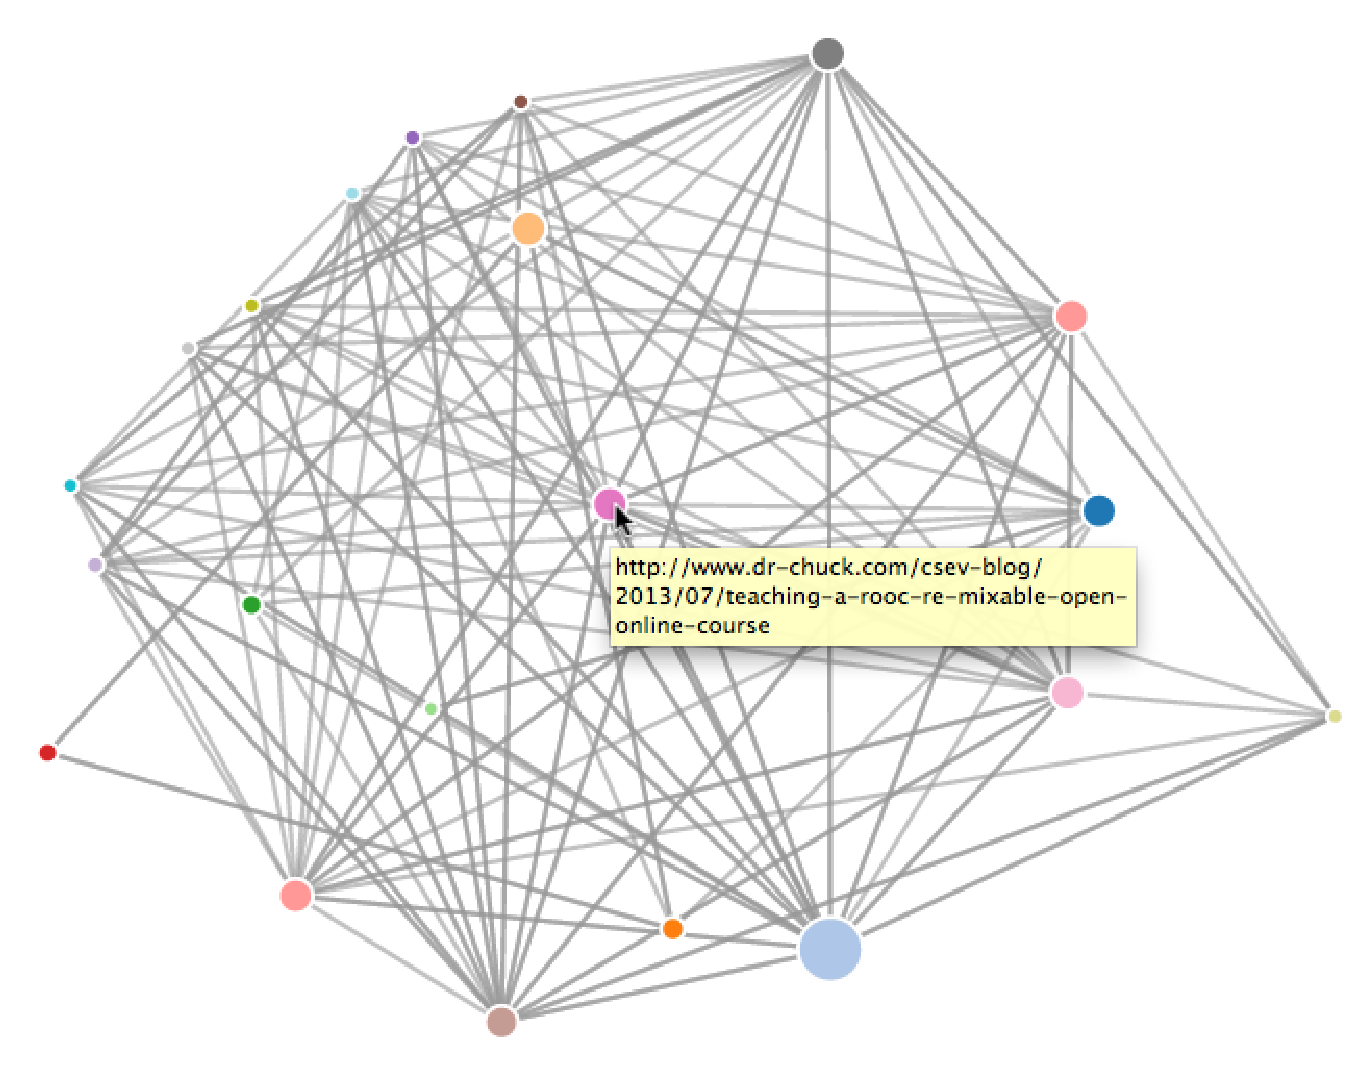
\includegraphics[height=2.25in]{figs2/pagerank.eps}}
\afterfig

O primeiro programa ({\bf spider.py}) vasculha páginas web e grava
uma série de páginas no banco de dados ({\bf spider.sqlite}), gravando
as ligações entre as páginas. Você pode reiniciar o processo a qualquer
hora deletando o arquivo {\bf spider.sqlite} e reexecutando o {\bf spider.py}.
%The first program ({\bf spider.py}) program crawls a web 
%site and pulls a series of pages into the
%database ({\bf spider.sqlite}), recording the links between pages.
%You can restart the process at any time by removing the 
%{\bf spider.sqlite} file and rerunning {\bf spider.py}.

\beforeverb
\begin{verbatim}
Enter web url or enter: http://www.dr-chuck.com/
['http://www.dr-chuck.com']
How many pages:2
1 http://www.dr-chuck.com/ 12
2 http://www.dr-chuck.com/csev-blog/ 57
How many pages:
\end{verbatim}
\afterverb
%

Neste exemplo de execução, nós pedimos ao programa para extrair e 
retornar duas páginas. Se você reiniciar o programa e pedir a ele para
obter mais páginas, não irá pegar novamente as mesmas páginas que já
estão no banco de dados. Após o restart ele vai sortear randomicamente
páginas e começar de lá. Assim, cada execução sucessiva do {\bf spider.py}
é um aditivo.
%In this sample run, we told it to crawl a website and retrieve two 
%pages.  If you restart the program and tell it to crawl more
%pages, it will not re-crawl any pages already in the database.  Upon 
%restart it goes to a random non-crawled page and starts there.  So 
%each successive run of {\bf spider.py} is additive.

\beforeverb
\begin{verbatim}
Enter web url or enter: http://www.dr-chuck.com/
['http://www.dr-chuck.com']
How many pages:3
3 http://www.dr-chuck.com/csev-blog 57
4 http://www.dr-chuck.com/dr-chuck/resume/speaking.htm 1
5 http://www.dr-chuck.com/dr-chuck/resume/index.htm 13
How many pages:
\end{verbatim}
\afterverb
%

Você pode ter múltiplos pontos de start no mesmo banco de dados, dentro
do programa, eles são chamados ``webs''. O programa escolhe randomicamente
um dos links que ainda não foi visitado através de toda a web como sendo
a próxima página a ser visitada.
%You can have multiple starting points in the same database---within
%the program, these are called ``webs''.   The spider
%chooses randomly amongst all non-visited links across all
%the webs as the next page to spider.

Se você quer visualizar o conteúdo do arquivo {\bf spider.sqlite}, você pode
rodar o programa {\bf spdump.py}, como segue:
%If you want to dump the contents of the {\bf spider.sqlite} file, you can 
%run {\bf spdump.py} as follows:

\beforeverb
\begin{verbatim}
(5, None, 1.0, 3, u'http://www.dr-chuck.com/csev-blog')
(3, None, 1.0, 4, u'http://www.dr-chuck.com/dr-chuck/resume/speaking.htm')
(1, None, 1.0, 2, u'http://www.dr-chuck.com/csev-blog/')
(1, None, 1.0, 5, u'http://www.dr-chuck.com/dr-chuck/resume/index.htm')
4 rows.
\end{verbatim}
\afterverb
%

Isto mostra o número de links visitados, o antigo page rank, o novo page
rank, o id da página, e a url da página. O programa {\bf spdump.py} somente
mostra páginas que tem pelo menos um link já visitado.
%This shows the number of incoming links, the old page rank, the new page
%rank, the id of the page, and the url of the page.  The {\bf spdump.py} program
%only shows pages that have at least one incoming link to them.

Uma vez que você tem algumas páginas no banco de dados, você pode rodar o page 
rank nas páginas usando o programa {\bf sprank.py}. Você apenas diz quantas
iterações de páginas devem ser executadas.
%Once you have a few pages in the database, you can run page rank on the
%pages using the {\bf sprank.py} program.  You simply tell it how many page
%rank iterations to run.

\beforeverb
\begin{verbatim}
How many iterations:2
1 0.546848992536
2 0.226714939664
[(1, 0.559), (2, 0.659), (3, 0.985), (4, 2.135), (5, 0.659)]
\end{verbatim}
\afterverb
%
Você pode analisar o banco de dados novamente para ver se o page rank foi
atualizado:
%You can dump the database again to see that page rank has been updated:

\beforeverb
\begin{verbatim}
(5, 1.0, 0.985, 3, u'http://www.dr-chuck.com/csev-blog')
(3, 1.0, 2.135, 4, u'http://www.dr-chuck.com/dr-chuck/resume/speaking.htm')
(1, 1.0, 0.659, 2, u'http://www.dr-chuck.com/csev-blog/')
(1, 1.0, 0.659, 5, u'http://www.dr-chuck.com/dr-chuck/resume/index.htm')
4 rows.
\end{verbatim}
\afterverb
%

Você pode rodar o {\bf sprank.py} quantas vezes quiser, isto irá apenas refinar
o page rank cada vez que você executar. Pode até mesmo rodar o {\bf sprank.py} um
pequeno número de vezes e então recuperar mais algumas páginas com o {\bf spider.py} 
e então rodar o {\bf sprank.py} para recuperar os valores do page rank. Um motor de
pesquisa geralmente roda os programas de recuperação e rankeamento ao mesmo tempo.
%You can run {\bf sprank.py} as many times as you like and it will simply refine
%the page rank each time you run it.  You can even run {\bf sprank.py} a few times
%and then go spider a few more pages sith {\bf spider.py} and then run {\bf sprank.py}
%to reconverge the page rank values.  A search engine usually runs both the crawling and 
%ranking programs all the time.

Se você quiser reiniciar os cálculos de page rank sem fazer a extração das páginas
web novamente, você pode usar o {\bf spreset.py} e então reiniciar o {\bf sprank.py}.
%If you want to restart the page rank calculations without respidering the 
%web pages, you can use {\bf spreset.py} and then restart {\bf sprank.py}.

\beforeverb
\begin{verbatim}
How many iterations:50
1 0.546848992536
2 0.226714939664
3 0.0659516187242
4 0.0244199333
5 0.0102096489546
6 0.00610244329379
...
42 0.000109076928206
43 9.91987599002e-05
44 9.02151706798e-05
45 8.20451504471e-05
46 7.46150183837e-05
47 6.7857770908e-05
48 6.17124694224e-05
49 5.61236959327e-05
50 5.10410499467e-05
[(512, 0.0296), (1, 12.79), (2, 28.93), (3, 6.808), (4, 13.46)]
\end{verbatim}
\afterverb
%

Para cada iteração do algoritmo de page rank, ele imprime a média
de modificações no page rank por página. A rede inicia-se
desbalanceada e então os valores do page rank individual mudam
com velocidade entre as iterações. Mas em poucas iterações, o page rank 
coverge. Você deve rodar o {\bf prank.py} por tempo suficiente para
que os valores de page rank possam convergir.
%For each iteration of the page rank algorithm it prints the average
%change in page rank per page.   The network initially is quite
%unbalanced and so the individual page rank values change wildly between
%iterations. But in a few short iterations, the page rank converges.  You
%should run {\bf prank.py} long enough that the page rank values converge.

Se você quer visualizar as primeiras páginas no rank, rode o {\bf spjson.py}
para ler o banco de dados e escrever os dados dos links com maior pontuação
no formato JSON para serem vistos no web browser.
%If you want to visualize the current top pages in terms of page rank,
%run {\bf spjson.py} to read the database and write the data for the 
%most highly linked pages in JSON format to be viewed in a
%web browser.

\beforeverb
\begin{verbatim}
Creating JSON output on spider.json...
How many nodes? 30
Open force.html in a browser to view the visualization
\end{verbatim}
\afterverb
%\beforeverb
%\begin{verbatim}
%Creating JSON output on spider.json...
%How many nodes? 30
%Open force.html in a browser to view the visualization
%\end{verbatim}
%\afterverb
%

Você pode visualizar este dado abrindo o arquivo {\bf force.html} em seu web 
browser. Isto mostra um layout automático de nós e links. Você pode clicar e
arrastar qualquer nó e também dar um duplo clique no nó para encontrar a URL
que ele representa.
%You can view this data by opening the file {\bf force.html} in your web browser.  
%This shows an automatic layout of the nodes and links.  You can click and 
%drag any node and you can also double-click on a node to find the URL
%that is represented by the node.

Se você rodar novamente algum script, lembre-se de rodar também o 
{\bf spjson.py} e pressionar o botão de refresh no browser para ler
os novos dados do arquivo {\bf spider.json}.
%If you rerun the other utilities, rerun {\bf spjson.py} and
%press refresh in the browser to get the new data from {\bf spider.json}.

\section{Visualizando dados de e-mail}
%\section{Visualizing mail data}

Até este ponto do livro, esperamos que você já se familiarizado com os 
nossos arquivos de dados, {\bf mbox-short.txt} e {\bf mbox.txt}. Agora
é hora de levar a nossa análise de e-mails para um próximo nível.
%Up to this point in the book, you have become quite familiar with our 
%{\bf mbox-short.txt} and {\bf mbox.txt} data files.   Now it is time to take
%our analysis of email data to the next level.  

No mundo real, às vezes você tem que puxar dados de e-mails dos servidores.
Isto pode levar um bom tempo e talvez o dado seja inconsistente, com erros
de preenchimento, e precisem de muitas limpezas e ajustes. Nesta seção, nós
trabalharemos com uma aplicação que é muito complexa e baixa aproximadamente
um gigabyte de dados e faz a leitura.
%In the real world, sometimes you have to pull down mail data from servers.
%That might take quite some time and the data might be inconsistent, 
%error-filled, and need a lot of cleanup or adjustment.  In this section, we
%work with an application that is the most complex so far and pull down nearly a 
%gigabyte of data and visualize it.

\beforefig
\centerline{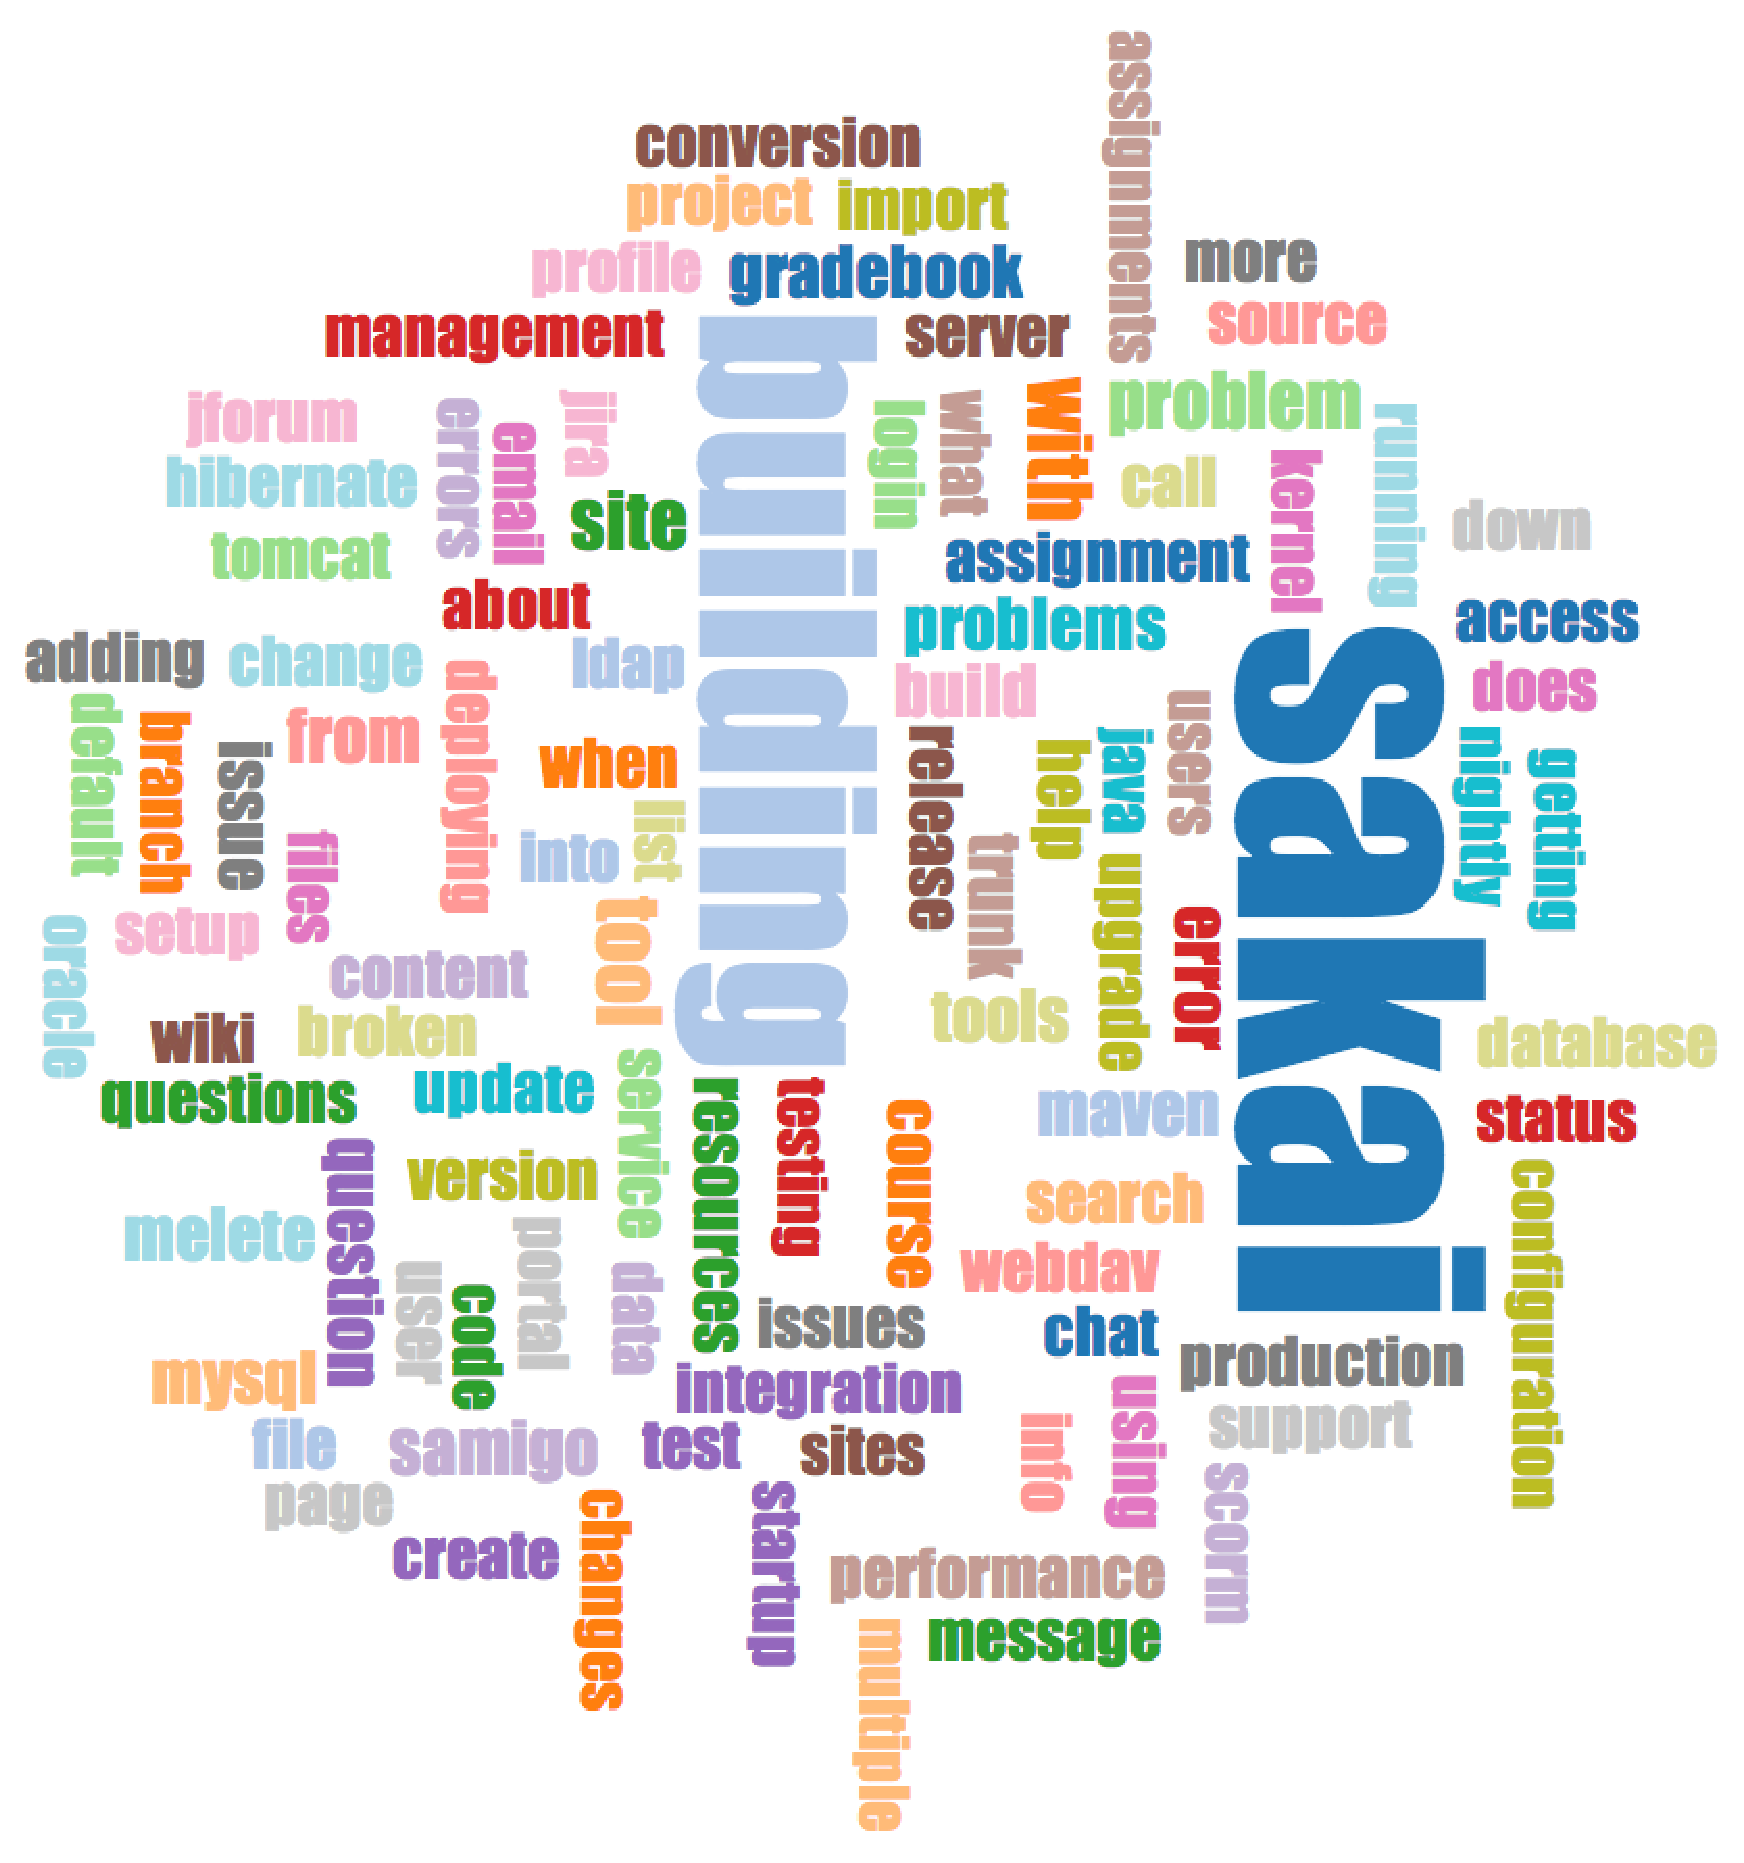
\includegraphics[height=2.50in]{figs2/wordcloud.eps}}
\afterfig

Você pode fazer o download desta aplicação em:
%You can download this application from:

\url{www.py4inf.com/code/gmane.zip}

Nós utilizaremos dados de um serviço de arquivamento de listas de e-mails
gratuita chamado \url{www.gmane.org}. Este serviço é muito popular em projetos
open source porque disponibiliza uma vasta coleção pesquisável de arquivos sobre
a atividade de email deles. Eles também tem uma política liberal em relação
ao acesso de seus dados através de sua API. Não tem taxas de limites, mas pedem
para que você não sobrecarregue os seus serviços e pegue apenas os dados
que você precise. Você pode ler os termos e condições do gname nesta página:
%We will be using data from a free email list archiving service called 
%\url{www.gmane.org}.  This service is very popular with open source
%projects because it provides a nice searchable archive of their 
%email activity.  They also have a very liberal policy regarding accessing 
%their data through their API.  They have no rate limits, but ask that you 
%don't overload their service and take only the data you need.  You can read
%gmane's terms and conditions at this page:

\url{http://gmane.org/export.php}

{\em É muito importante que você faça uso dos dados do gname.org com
responsabilidade adicionando delays no acesso ao serviço deles e 
espalhando tarefas de longa duração em um longo período de tempo.
Não abuse deste serviço gratuito, arruinando-o para o resto de nós.}
%{\em It is very important that you make use of the gmane.org data
%responsibly by adding delays to your access of their services and spreading
%long-running jobs over a longer period of time.  Do not abuse this free service
%and ruin it for the rest of us.}

Quando os dados de email do Sakai foram vasculhados usando este software, 
produziu aproximadamente um Gigabyte de dados e executou muitas vezes 
durante vários dias.
O arquivo {\bf README.txt} no arquivo ZIP acima, pode ter instruções sobre
como você pode fazer download de uma cópia preparada previamente através do
arquivo {\bf content.sqlite} para a maioria dos corpos dos emails Sakai, assim
você não precisa coletar os dados por cinco dias apenas para rodar seus programas.
Se você baixar conteúdos pré preparados, você ainda pode rodar o processo de coleta
para pegar mensagens mais recentes.
%When the Sakai email data was spidered using this software, it produced nearly 
%a Gigabyte of data and took a number of runs on several days.
%The file {\bf README.txt} in the above ZIP may have instructions as to how
%you can download a pre-spidered copy of the {\bf content.sqlite} file for 
%a majority of the Sakai email corpus so you don't have to spider for 
%five days just to run the programs.  If you download the pre-spidered
%content, you should still run the spidering process to catch up with 
%more recent messages.

O primeiro passo é fazer uma coleta no repositório gname. A URL base
está fixa dentro do arquivo {\bf gmane.py} e está apontando para a lista
de desenvolvedores do Sakai. Você pode coletar outro repositório apenas
mudando a url base. Certifique-se de deletar o arquivo {\bf content.sqlite}
se você trocar a url base.
%The first step is to spider the gmane repository.  The base URL 
%is hard-coded in the {\bf gmane.py} and is hard-coded to the Sakai
%developer list.  You can spider another repository by changing that
%base url.   Make sure to delete the {\bf content.sqlite} file if you 
%switch the base url.  

O arquivo {\bf gmane.py} funciona como um cache spider responsável,
executando lentamente e retornando uma mensagem de e-mail por segundo,
não sendo bloqueado desta forma pelo site gname. Ele armazena todos os
seus dados em um banco de dados e pode ser interrompido e reiniciado
quantas vezes forem necessárias. Pode levar muitas horas para baixar
todos os dados. Você pode precisar reiniciar muitas vezes.
%The {\bf gmane.py} file operates as a responsible caching spider in 
%that it runs slowly and retrieves one mail message per second so 
%as to avoid getting throttled by gmane.   It stores all of
%its data in a database and can be interrupted and restarted 
%as often as needed.   It may take many hours to pull all the data
%down.  So you may need to restart several times.

Aqui está uma execução do {\bf gmane.py} retornando as últimas cinco 
mensagens da lista de desenvolvedores do Sakai:
%Here is a run of {\bf gmane.py} retrieving the last five messages of the
%Sakai developer list:

\beforeverb
\begin{verbatim}
How many messages:10
http://download.gmane.org/gmane.comp.cms.sakai.devel/51410/51411 9460
    nealcaidin@sakaifoundation.org 2013-04-05 re: [building ...
http://download.gmane.org/gmane.comp.cms.sakai.devel/51411/51412 3379
    samuelgutierrezjimenez@gmail.com 2013-04-06 re: [building ...
http://download.gmane.org/gmane.comp.cms.sakai.devel/51412/51413 9903
    da1@vt.edu 2013-04-05 [building sakai] melete 2.9 oracle ...
http://download.gmane.org/gmane.comp.cms.sakai.devel/51413/51414 349265
    m.shedid@elraed-it.com 2013-04-07 [building sakai] ...
http://download.gmane.org/gmane.comp.cms.sakai.devel/51414/51415 3481
    samuelgutierrezjimenez@gmail.com 2013-04-07 re: ...
http://download.gmane.org/gmane.comp.cms.sakai.devel/51415/51416 0

Does not start with From 
\end{verbatim}
\afterverb
%

O programa escaneia o {\bf content.sqlite} e inicia a execução a partir da primeira
mensagem que ainda não foi processada. Ele continua coletando até chegar ao número
desejado de mensagens ou atingir uma página que possuir uma mensagem fora do padrão.
%The program scans {\bf content.sqlite} from one up to the first message number not
%already spidered and starts spidering at that message.  It continues spidering
%until it has spidered the desired number of messages or it reaches a page
%that does not appear to be a properly formatted message.

Às vezes o \url{gmane.org} perde alguma mensagem. Seja pelos administradores que deletaram
uma mensagem ou então perdeu-se mesmo. Se seu programa para, e parece que ele perdeu alguma 
mensagem, vá para o administrador SQLite e adicione uma linha com o id que está faltando,
deixando todos os outros campos em branco e reinicie o {\bf gmane.py}. Isto irá liberar o 
seu programa para continuar a execução. Estas mensagens vazias serão ignoradas na próxima 
fase do processo.
%Sometimes \url{gmane.org} is missing a message.  Perhaps administrators can delete messages
%or perhaps they get lost.   If your spider stops, and it seems it has hit
%a missing message, go into the SQLite Manager and add a row with the missing id leaving
%all the other fields blank and restart {\bf gmane.py}.   This will unstick the 
%spidering process and allow it to continue.  These empty messages will be ignored in the next
%phase of the process.

Uma coisa legal é que uma vez que você coletou todas as mensagens e tem elas dentro do
{\bf content.sqlite}, você pode rodar o {\bf gmane.py} novamente para pegar as últimas 
mensagens novas enviadas para a lista.
%One nice thing is that once you have spidered all of the messages and have them in 
%{\bf content.sqlite}, you can run {\bf gmane.py} again to get new messages as 
%they are sent to the list.  

O dados do {\bf content.sqlite} são um pouco cru, com um modelo de dados ineficiente
e não comprimido.
Isto é intencional pois permite a você olhar o conteúdo do {\bf content.sqlite}
no SQLite Manager para debugar problemas que ocorreram no processo de coleta.
Seria uma má idéia rodar qualquer tipo de consulta neste banco de dados, pois
poderia demorar.  
%The {\bf content.sqlite} data is pretty raw, with an inefficient data model, 
%and not compressed.
%This is intentional as it allows you to look at {\bf content.sqlite}
%in the SQLite Manager to debug problems with the spidering process.
%It would be a bad idea to run any queries against this database, as they 
%would be quite slow.

O segundo processo é rodar o programa {\bf gmodel.py}. Este programa lê os dados crus do
{\bf content.sqlite} e produz uma versão bem modelada dos dados no arquivo {\bf index.sqlite}.
Este arquivo será muito menor (quase 10 vezes menor) do que o {\bf index.sqlite}, porque 
comprime o corpo e o cabeçalho do texto.
%The second process is to run the program {\bf gmodel.py}.  This program reads the raw 
%data from {\bf content.sqlite} and produces a cleaned-up and well-modeled version of the 
%data in the file {\bf index.sqlite}.  This file will be much smaller (often 10X
%smaller) than {\bf content.sqlite} because it also compresses the header and body text.

Cada vez que o {\bf gmodel.py} roda, ele deleta e refaz o arquivo {\bf index.sqlite},
permitindo a você ajustar os parâmetros e editar as tabelas de mapeamento no {\bf content.sqlite}
para ajustar o processo de limpeza dos dados. Esta é uma amostra da execução do {\bf gmodel.py}.
Ele imprime uma linha por vez, 250 mensagens de email são processadas, assim você pode ver
algum progresso acontecendo, como este programa pode rodar por um longo tempo, é muito
fácil conseguir um arquivo de e-mail de um Gigabyte de dados.
%Each time {\bf gmodel.py} runs it deletes and rebuilds {\bf index.sqlite}, allowing
%you to adjust its parameters and edit the mapping tables in {\bf content.sqlite} to tweak the 
%data cleaning process. This is a sample run of {\bf gmodel.py}.  It prints a line out each time
%250 mail messages are processed so you can see some progress happening, as this program may
%run for a while processing nearly a Gigabyte of mail data.

\beforeverb
\begin{verbatim}
Loaded allsenders 1588 and mapping 28 dns mapping 1
1 2005-12-08T23:34:30-06:00 ggolden22@mac.com
251 2005-12-22T10:03:20-08:00 tpamsler@ucdavis.edu
501 2006-01-12T11:17:34-05:00 lance@indiana.edu
751 2006-01-24T11:13:28-08:00 vrajgopalan@ucmerced.edu
...
\end{verbatim}
\afterverb
%

O programa {\bf gmodel.py} trata um número de tarefas de limpeza de dados.
%The {\bf gmodel.py} program handles a number of data cleaning tasks.

Nomes de domínios são truncados para dois níveis para .com, .org, .edu, e .net. 
Outros nomes de domínios são truncados para três níveis. Assim si.umich.edu
se transforma em umich.edu e caret.cam.ac.uk se transforma em cam.ac.uk.
Endereços de email também são forçados para minúsculo, seguem alguns endereços
do @gmane.org, por exemplo:
%Domain names are truncated to two levels for .com, .org, .edu, and .net.
%Other domain names are truncated to three levels.  So si.umich.edu becomes
%umich.edu and caret.cam.ac.uk becomes cam.ac.uk.   Email addresses are also
%forced to lower case, and some of the @gmane.org address like the following

\beforeverb
\begin{verbatim}
   arwhyte-63aXycvo3TyHXe+LvDLADg@public.gmane.org
\end{verbatim}
\afterverb
%

são convertidos para endereços reais a qualquer hora que ocorrer um encontro
real de endereço de email em qualquer lugar no corpo da mensagem. 
%are converted to the real address whenever there is a matching real email
%address elsewhere in the message corpus.

No banco de dados {\bf content.sqlite}, há duas tabelas que permitem a você
mapear ambos os nomes de domínio e os endereços de email individuais que mudam
ao longo do tempo da lista. Por exemplo, Steve Githens usou os seguintes endereços 
de e-mail conforme foi mudando de emprego na lista de desenvolvedores Sakai:
%In the {\bf content.sqlite} database there are two tables that allow
%you to map both domain names and individual email addresses that change over 
%the lifetime of the email list.  For example, Steve Githens used the following
%email addresses as he changed jobs over the life of the Sakai developer list:

\beforeverb
\begin{verbatim}
s-githens@northwestern.edu
sgithens@cam.ac.uk
swgithen@mtu.edu
\end{verbatim}
\afterverb
%

Nós podemos adicionar duas entradas na tabela de mapeamento em {\bf content.sqlite},
assim o {\bf gmodel.py} irá mapear todos os três para um único endereço: 
%We can add two entries to the Mapping table in {\bf content.sqlite} so 
%{\bf gmodel.py} will map all three to one address:

\beforeverb
\begin{verbatim}
s-githens@northwestern.edu ->  swgithen@mtu.edu
sgithens@cam.ac.uk -> swgithen@mtu.edu
\end{verbatim}
\afterverb
%

Você pode criar entradas similares na tabela de mapeamento DNS se possuir múltiplos
nomes DNS mapeados para um DNS simples. O seguinte mapeamento foi adicionado para os 
dados Sakai: 
%You can also make similar entries in the DNSMapping table if there are multiple
%DNS names you want mapped to a single DNS.  The following mapping was added to the Sakai data:

\beforeverb
\begin{verbatim}
iupui.edu -> indiana.edu
\end{verbatim}
\afterverb
%

assim todas as contas de vários campus da Universidade de Indiana são atreladas juntas.
%so all the accounts from the various Indiana University campuses are tracked together.

Você pode reexecutar o {\bf gmodel.py} de novo e de novo conforme olhar para os dados e 
adicionar mapeamentos para tornar os dados mais limpos. Quando você acabar, você terá uma
agradável versão indexada dos emails em {\bf index.sqlite}. Este é o arquivo para se fazer
análise dos dados. Com este arquivo, a análise dos dados será muito rápida. 
%You can rerun the {\bf gmodel.py} over and over as you look at the data, and add mappings
%to make the data cleaner and cleaner.   When you are done, you will have a nicely
%indexed version of the email in {\bf index.sqlite}.   This is the file to use to do data
%analysis.   With this file, data analysis will be really quick.

A primeira, análise simples dos dados é para determinar "quem enviou mais emails?" e 
"qual organização enviou mais emails?" Isto é feito usando o {\bf gbasic.py}:  
%The first, simplest data analysis is to determine "who sent the most mail?" and "which 
%organization sent the most mail"?  This is done using {\bf gbasic.py}:

\beforeverb
\begin{verbatim}
How many to dump? 5
Loaded messages= 51330 subjects= 25033 senders= 1584

Top 5 Email list participants
steve.swinsburg@gmail.com 2657
azeckoski@unicon.net 1742
ieb@tfd.co.uk 1591
csev@umich.edu 1304
david.horwitz@uct.ac.za 1184

Top 5 Email list organizations
gmail.com 7339
umich.edu 6243
uct.ac.za 2451
indiana.edu 2258
unicon.net 2055
\end{verbatim}
\afterverb
%

Observe quão mais rápido o {\bf gbasic.py} executa quando comparado ao {\bf gmane.py}
ou até mesmo ao {\bf gmodel.py}. Eles todos trabalham no mesmo dado, mas o {\bf gbasic.py}
está usando dados normalizados e comprimidos em {\bf index.sqlite}. Se você tiver
muitos dados para gerenciar, um processo multi passos assim como estes nesta aplicação
podem levar mais tempo para serem desenvolvidos, mas irão economizar muito tempo
quando você começar a explorar e visualizar os seus dados.
%Note how much more quickly {\bf gbasic.py} runs compared to {\bf gmane.py}
%or even {\bf gmodel.py}. They are all working on the same data, but 
%{\bf gbasic.py} is using the compressed and normalized data in 
%{\bf index.sqlite}.  If you have a lot of data to manage, a multistep
%process like the one in this application may take a little longer to develop,
%but will save you a lot of time when you really start to explore
%and visualize your data.

Você pode produzir uma simples visualização da frequência das palavras nas
linhas do arquivo {\bf gword.py}: 
%You can produce a simple visualization of the word frequency in the subject lines
%in the file {\bf gword.py}:

\beforeverb
\begin{verbatim}
Range of counts: 33229 129
Output written to gword.js
\end{verbatim}
\afterverb
%

Isto produz o arquivo {\bf gword.js}, o qual você pode visualizar usando
o {\bf gword.htm} para produzir uma nuvem de palavras similares àquelas
no início desta seção.
%This produces the file {\bf gword.js} which you can visualize using
%{\bf gword.htm} to produce a word cloud similar to the one at the beginning 
%of this section.

Uma segunda visualização foi produzida pelo {\bf gline.py}. Ele computa a 
participação das organizações por email ao longo do tempo. 
%A second visualization is produced  by {\bf gline.py}.  It computes email 
%participation by organizations over time.

\beforeverb
\begin{verbatim}
Loaded messages= 51330 subjects= 25033 senders= 1584
Top 10 Oranizations
['gmail.com', 'umich.edu', 'uct.ac.za', 'indiana.edu', 
'unicon.net', 'tfd.co.uk', 'berkeley.edu', 'longsight.com', 
'stanford.edu', 'ox.ac.uk']
Output written to gline.js
\end{verbatim}
\afterverb
%

Sua saída é escrita para {\bf gline.js}, o qual é visualizada usando {\bf gline.htm}.
%Its output is written to {\bf gline.js} which is visualized using {\bf gline.htm}.

\beforefig
\centerline{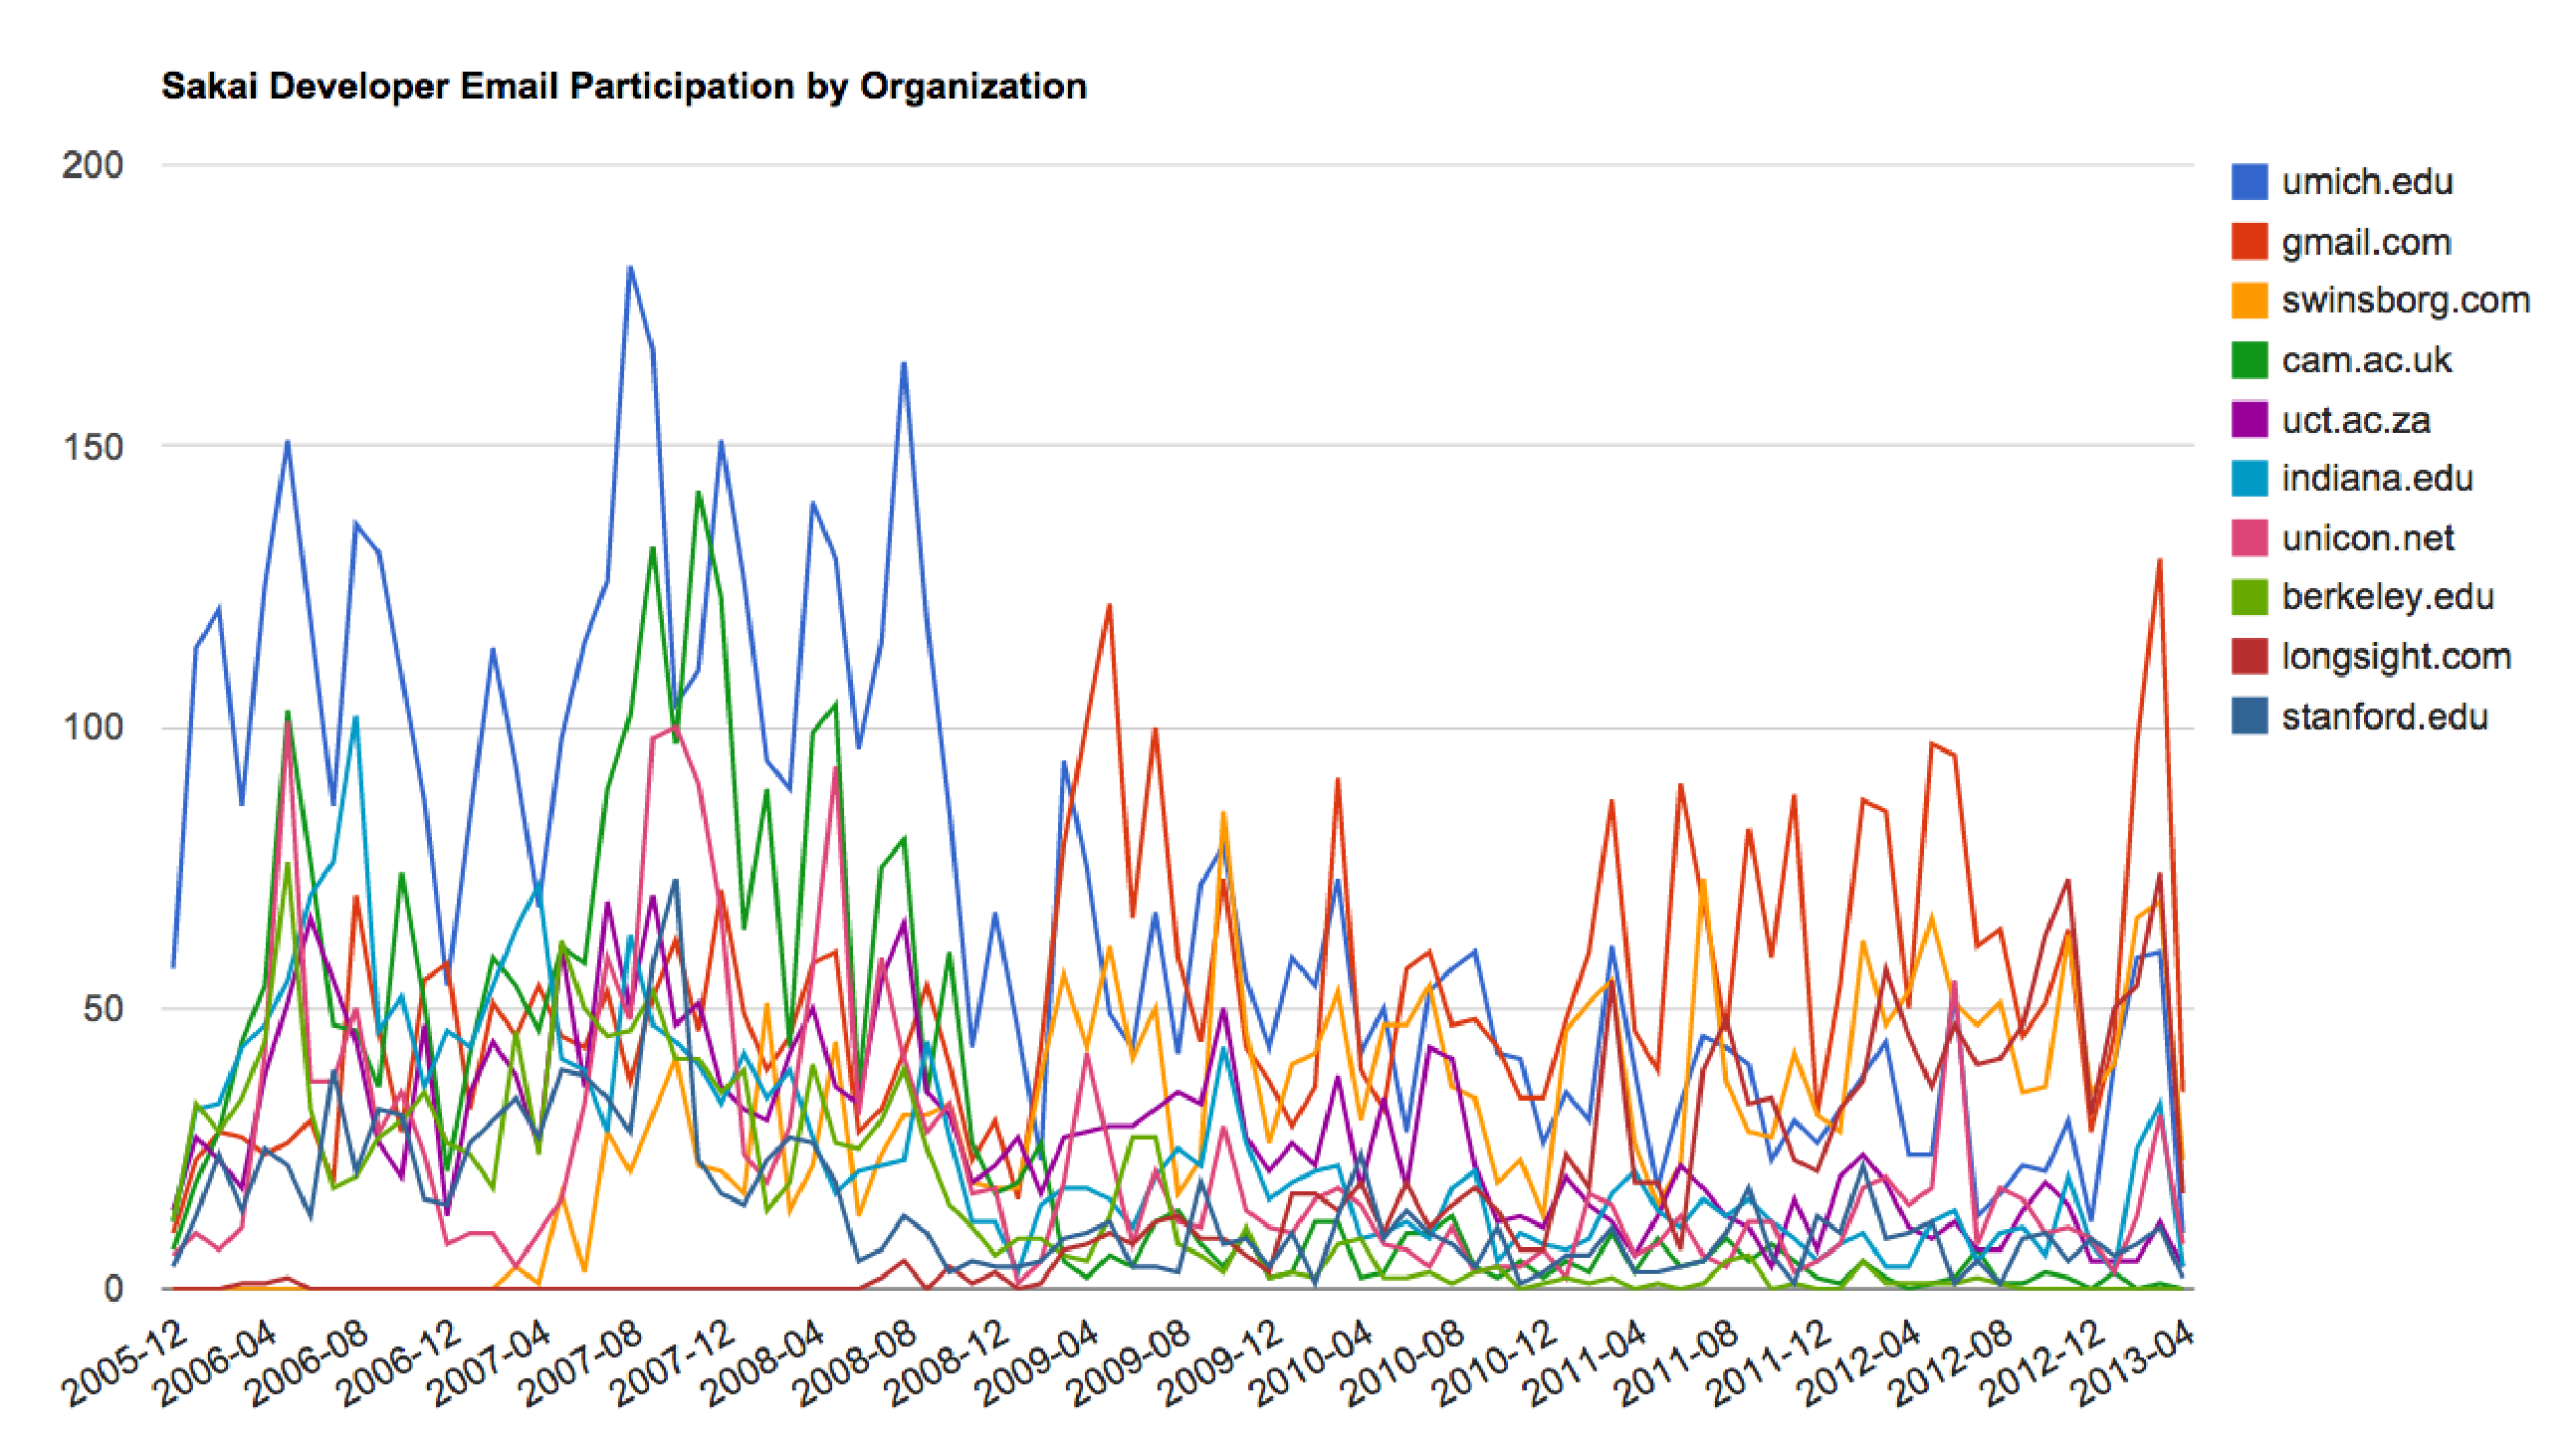
\includegraphics[height=2.50in]{figs2/mailorg.eps}}
\afterfig

Esta é uma aplicação relativamente complexa e sofisticada e têm características
para fazer uma coleta real de dados, limpeza e visualização. 
%This is a relatively complex and sophisticated application and 
%has features to do some real data retrieval, cleaning, and visualization.

% The contents of this file is 
% Copyright (c) 2009-  Charles R. Severance, All Righs Reserved

\chapter{Automação de tarefas comuns no seu computador}
%\chapter{Automating common tasks on your computer}

Temos lido dados de arquivos, redes, serviços e banco de dados.
Python também pode navegar através de todas as pastas e diretórios 
no seu computador e ler os arquivos também.
%We have been reading data from files, networks, services,
%and databases.   Python can also go through all of the 
%directories and folders on your computers and read those files
%as well.

Neste capítulo, nós iremos escrever programas que analisam o seu computador e executam algumas operações em seus arquivos. Arquivos são organizados em diretórios (também chamados de pastas).
Scripts Python simples podem fazer o trabalho de tarefas simples que devem ser feitas em
centenas ou milhares de arquivos espalhados por uma árvore de diretórios ou todo o seu computador.
%In this chapter, we will write programs that scan 
%through your computer and 
%perform some operation on each file.  
%Files are organized into directories (also called ``folders'').
%Simple Python scripts
%can make short work of simple tasks that must be done to 
%hundreds or thousands of files
%spread across a directory tree or your entire computer.

Para navegar através de todos os diretórios e arquivos em uma árvore nós utilizamos 
{\tt os.walk} e um laço de repetição {\tt for}. Isto é similar ao comando {\tt open} e nos permite escrever um laço de repetição para ler o conteúdo de um arquivo, {\tt socket} nos permite escrever um laço de repetição para ler o conteúdo de uma conexão e {\tt urllib} nos permite abrir um documento web e navegar por meio de um laço de repetição no seu conteúdo. 
%To walk through all the directories and files in a tree we use 
%{\tt os.walk} and a {\tt for} loop.  This is similar to how 
%{\tt open} allows us to write a loop to read the contents of a file,
%{\tt socket} allows us to write a loop to read the contents of a network connection, and
%{\tt urllib} allows us to open a web document and loop through its contents.

\section{Nomes e caminhos de arquivos}
\label{paths}
%\section{File names and paths}
%\label{paths}

\index{file name}
\index{path}
\index{directory}
\index{folder}
%\index{file name}
%\index{path}
%\index{directory}
%\index{folder}

{\it Todo programa em execução tem um ``diretório atual'' que é o diretório padrão para a maioria das operações. Por exemplo, quando você abre um arquivo para leitura, o Python o procura no diretório atual.}
%Every running program has a ``current directory,'' which is the
%default directory for most operations.  For example, when you open a file
%for reading, Python looks for it in the current directory.

\index{os module}
\index{module!os}
%\index{os module}
%\index{module!os}

O módulo {\tt os} disponibiliza funções para trabalhar com arquivos e diretórios ({\tt os} do inglês "operating system" que significa sistema operacional).  
{\tt os.getcwd} retorna o nome do diretório atual:
%The {\tt os} module provides functions for working with files and
%directories ({\tt os} stands for ``operating system'').  {\tt os.getcwd}
%returns the name of the current directory:

\index{getcwd function}
\index{function!getcwd}
%\index{getcwd function}
%\index{function!getcwd}

\beforeverb
\begin{verbatim}
>>> import os
>>> cwd = os.getcwd()
>>> print cwd
/Users/csev
\end{verbatim}
\afterverb
%\beforeverb
%\begin{verbatim}
%>>> import os
%>>> cwd = os.getcwd()
%>>> print cwd
%/Users/csev
%\end{verbatim}
%\afterverb
%
{\tt cwd} significa {\bf diretório atual de trabalho}. O resultado neste exemplo é 
{\tt /Users/csev}, que é o diretório home do usuário chamado {\tt csev}.
%{\tt cwd} stands for {\bf current working directory}.  The result in
%this example is {\tt /Users/csev}, which is the home directory of a
%user named {\tt csev}.

\index{working directory}
\index{directory!working}
%\index{working directory}
%\index{directory!working}

Uma string {\tt cwd} que identifica um arquivo é chamado de path.
Um {\bf caminho relativo} é relativo ao diretório atual (corrente);
Um {\bf caminho absoluto} tem inicio no diretório raiz do sistema de arquivos.
%A string like {\tt cwd} that identifies a file is called a path.
%A {\bf relative path} starts from the current directory;
%an {\bf absolute path} starts from the topmost directory in the
%file system.

\index{relative path}
\index{path!relative}
\index{absolute path}
\index{path!absolute}
%\index{relative path}
%\index{path!relative}
%\index{absolute path}
%\index{path!absolute}

Os caminhos que temos visto até agora são nomes de arquivos simples, por isso são relativos ao diretório atual. Para encontrar o caminho absoluto de um arquivo, você pode usar {\tt os.path.abspath}:
%The paths we have seen so far are simple file names, so they are
%relative to the current directory.  To find the absolute path to
%a file, you can use {\tt os.path.abspath}:

\beforeverb
\begin{verbatim}
>>> os.path.abspath('memo.txt')
'/Users/csev/memo.txt'
\end{verbatim}
\afterverb
%\beforeverb
%\begin{verbatim}
%>>> os.path.abspath('memo.txt')
%'/Users/csev/memo.txt'
%\end{verbatim}
%\afterverb

{\tt os.path.exists} verifica se um determinado arquivo existe:
%{\tt os.path.exists} checks
%whether a file or directory exists:

\index{exists function}
\index{function!exists}
%\index{exists function}
%\index{function!exists}

\beforeverb
\begin{verbatim}
>>> os.path.exists('memo.txt')
True
\end{verbatim}
\afterverb
%\beforeverb
%\begin{verbatim}
%>>> os.path.exists('memo.txt')
%True
%\end{verbatim}
%\afterverb

Se existir, {\tt os.path.isdir} verifica se é um diretório:
%If it exists, {\tt os.path.isdir} checks whether it's a directory:

\beforeverb
\begin{verbatim}
>>> os.path.isdir('memo.txt')
False
>>> os.path.isdir('music')
True
\end{verbatim}
\afterverb
%\beforeverb
%\begin{verbatim}
%>>> os.path.isdir('memo.txt')
%False
%>>> os.path.isdir('music')
%True
%\end{verbatim}
%\afterverb

Da mesma forma, {\tt os.path.isfile} verifica se é um arquivo.
%Similarly, {\tt os.path.isfile} checks whether it's a file.

{\tt os.listdir} retorna uma lista com os arquivos (e outros diretórios) do diretório informado:
%{\tt os.listdir} returns a list of the files (and other directories)
%in the given directory:

\beforeverb
\begin{verbatim}
>>> os.listdir(cwd)
['musicas', 'fotos', 'memo.txt']
\end{verbatim}
\afterverb
%\beforeverb
%\begin{verbatim}
%>>> os.listdir(cwd)
%['music', 'photos', 'memo.txt']
%\end{verbatim}
%\afterverb

\section{Exemplo: Limpando um diretório de fotos}
%\section{Example: Cleaning up a photo directory}

Há algum tempo atrás, desenvolvi um pequeno software tipo Flickr que recebe fotos do meu celular e armazena essas fotos no meu servidor. E escrevi isto antes do Flickr existir e continuo usando por que eu quero manter copias das minhas imagens originais para sempre.
%Some time ago, I built a bit of Flickr-like software that 
%received photos from my cell phone and stored those photos
%on my server.  I wrote this before Flickr existed and kept 
%using it after Flickr existed because I wanted to keep original
%copies of my images forever.

Eu também gostaria de enviar uma simples descrição numa mensagem MMS ou como um título de uma mensagem de e-mail. Eu armazenei essas mensagens em um arquivo de texto no mesmo diretório do arquivo das imagens. Eu criei uma estrutura de diretórios baseada no mês, ano, dia e hora no qual a foto foi tirada, abaixo um exemplo de nomenclatura para uma foto e sua descrição:
%I would also send a simple one-line text description in the MMS message
%or the subject line of the email message.  I stored these messages
%in a text file in the same directory as the image file.   I came up 
%with a directory structure based on the month, year, day, and time the 
%photo was taken.   The following would be an example of the naming for 
%one photo and its existing description:

\beforeverb
\begin{verbatim}
./2006/03/24-03-06_2018002.jpg
./2006/03/24-03-06_2018002.txt
\end{verbatim}
\afterverb
%\beforeverb
%\begin{verbatim}
%./2006/03/24-03-06_2018002.jpg
%./2006/03/24-03-06_2018002.txt
%\end{verbatim}
%\afterverb

Após sete anos, eu tenho muitas fotos e legendas. Ao longo dos anos como eu troquei de celular, algumas vezes, meu código para extrair a legenda para uma mensagem quebrou e adicionou um bando de dados inúteis no meu servidor ao invés de legenda.
%After seven years, I had a lot of photos and captions.  Over the years
%as I switched cell phones, sometimes my code to extract the caption from the message 
%would break and add a bunch of useless data on my server instead of a caption.  

Eu queria passar por estes arquivos e descobrir quais dos arquivos texto eram realmente legendas e quais eram lixo e, em seguida, apagar os arquivos que eram lixo. A primeira coisa a fazer foi conseguir um simples inventário dos arquivos texto que eu tinha em uma das subpastas usando o seguinte programa:
%I wanted to go through these files and figure out which of the 
%text files were really captions and which were junk and then delete the bad
%files.  The first thing to do was to get a simple inventory of 
%how many text files I had in one the subfolders
%using the following program:

\beforeverb
\begin{verbatim}
import os
count = 0
for (dirname, dirs, files) in os.walk('.'):
   for filename in files:
       if filename.endswith('.txt') :
           count = count + 1
print 'Files:', count

python txtcount.py
Files: 1917
\end{verbatim}
\afterverb
%\beforeverb
%\begin{verbatim}
%import os
%count = 0
%for (dirname, dirs, files) in os.walk('.'):
%   for filename in files:
%       if filename.endswith('.txt') :
%           count = count + 1
%print 'Files:', count
%
%python txtcount.py
%Files: 1917
%\end{verbatim}
%\afterverb

O segredo para um código tão pequeno é a utilização da biblioteca {\tt os.walk} do Python. Quando nós chamamos
{\tt os.walk} e inicializamos um diretório, ele "caminha" através de todos os diretórios e subdiretórios recursivamente.
O caractere ""."" indica para iniciar no diretório corrente e navegar para baixo.
Assim que encontra cada diretório, temos três valores em uma tupla no corpo do laço de repetição {\tt for}.
O primeiro valor é o diretório corrente, o segundo é uma lista de sub-diretórios e o terceiro valor é uma lista de arquivos no diretório corrente.
%The key bit of code that makes this possible is the {\tt os.walk}
%library in Python.  When we call {\tt os.walk} and give it a starting
%directory, it will ``walk'' through all of the directories 
%and subdirectories recursively.   The string ``.'' indicates
%to start in the current directory and walk downward.
%As it encounters each directory, we get three values in a tuple in the
%body of the {\tt for} loop.  The first value is the current
%directory name, the second value is the list of subdirectories 
%in the current directory, and the third value is a list of files
%in the current directory.

Nós não temos que procurar explicitamente dentro de cada diretório por que nós podemos contar com {\tt os.walk} para visitar eventualmente todas as pastas mas, nós queremos procurar em cada arquivo, então, escrevemos um simples laço de repetição {\tt for} para examinar cada um dos arquivos no diretório corrente. Vamos verificar se cada arquivo termina com ".txt" e depois contar o número de arquivos através de toda a árvore de diretórios que terminam com o sufixo ".txt".
%We do not have to explicitly look into each of the subdirectories
%because we can count on {\tt os.walk} to visit every 
%folder eventually.  But we do want to look at each file, so 
%we write a simple {\tt for} loop to examine each of the files 
%in the current directory.   We check each file to see if 
%it ends with ``.txt'' and then count the number of 
%files through the whole directory tree that end with the
%suffix ``.txt''.

Uma vez que nós temos uma noção da quantidade de arquivos terminados com ".txt", a próxima coisa a se fazer é tentar determinar  automaticamente no Python quais arquivos são maus e quais são bons. Para isto, escreveremos um programa simples para imprimir os arquivos e seus tamanhos.
%Once we have a sense of how many files end with ``.txt'', the next
%thing to do is try to automatically
%determine in Python which files are bad and which files
%are good.   So we write a simple program to print out the
%files and the size of each file:

\beforeverb
\begin{verbatim}
import os
from os.path import join
for (dirname, dirs, files) in os.walk('.'):
   for filename in files:
       if filename.endswith('.txt') :
           thefile = os.path.join(dirname,filename)
           print os.path.getsize(thefile), thefile
\end{verbatim}
\afterverb
%\beforeverb
%\begin{verbatim}
%import os
%from os.path import join
%for (dirname, dirs, files) in os.walk('.'):
%   for filename in files:
%       if filename.endswith('.txt') :
%           thefile = os.path.join(dirname,filename)
%           print os.path.getsize(thefile), thefile
%\end{verbatim}
%\afterverb

Agora, em vez de apenas contar os arquivos, criamos um nome de arquivo concatenando o nome do diretório com
o nome do arquivo dentro do diretório usando {\tt os.path.join}.
É importante usar o {\tt os.path.join} para concatenar a sequência de caracteres por que no Windows usamos a
barra invertida para construir os caminhos de arquivos e no Linux ou Apple nós usamos a barra (\verb"/") para construir o caminho do arquivo.
O {\tt os.path.join} conhece essas diferenças e sabe qual sistema esta rodando dessa forma, faz a concatenação mais adequada considerando o sistema. Então, o mesmo código em Python roda tando no Windows quanto em sistemas tipo Unix.
%Now instead of just counting the files, we create 
%a file name by concatenating the directory name with
%the name of the file within the directory using
%{\tt os.path.join}.   It is important to use 
%{\tt os.path.join} instead of string concatenation 
%because on Windows we use a backslash
%(\verb"\") to construct file paths and on Linux
%or Apple we use a forward slash (\verb"/") 
%to construct file paths.  The {\tt os.path.join}
%knows these differences and knows what system
%we are running on and it does the proper concatenation
%depending on the system.  So the same Python code
%runs on either Windows or Unix-style systems.

Uma vez que temos o nome completo do arquivo com o caminho do diretório, nós usamos o utilitário {\tt os.path.getsize} para pegar e imprimir o tamanho, produzindo a seguinte saída.  
%Once we have the full file name with directory
%path, we use the {\tt os.path.getsize} utility
%to get the size and print it out, producing the 
%following output:

\beforeverb
\begin{verbatim}
python txtsize.py
...
18 ./2006/03/24-03-06_2303002.txt
22 ./2006/03/25-03-06_1340001.txt
22 ./2006/03/25-03-06_2034001.txt
...
2565 ./2005/09/28-09-05_1043004.txt
2565 ./2005/09/28-09-05_1141002.txt
...
2578 ./2006/03/27-03-06_1618001.txt
2578 ./2006/03/28-03-06_2109001.txt
2578 ./2006/03/29-03-06_1355001.txt
...
\end{verbatim}
\afterverb
%\beforeverb
%\begin{verbatim}
%python txtsize.py
%...
%18 ./2006/03/24-03-06_2303002.txt
%22 ./2006/03/25-03-06_1340001.txt
%22 ./2006/03/25-03-06_2034001.txt
%...
%2565 ./2005/09/28-09-05_1043004.txt
%2565 ./2005/09/28-09-05_1141002.txt
%...
%2578 ./2006/03/27-03-06_1618001.txt
%2578 ./2006/03/28-03-06_2109001.txt
%2578 ./2006/03/29-03-06_1355001.txt
%...
%\end{verbatim}
%\afterverb

Analisando a saída, nós percebemos que alguns arquivos são bem pequenos e muitos dos arquivos são bem grandes e com o mesmo tamanho (2578 e 2565). Quando observamos alguns desses arquivos maiores manualmente, parece que os arquivos grandes são nada mais que HTML genérico idênticos que vinham de e-mails enviados para meu sistema a partir do meu próprio telefone:
%Scanning the output, we notice that some files are pretty short and 
%a lot of the files are pretty large and the same size (2578 and 2565). 
%When we take a look at a few of these larger files by hand, 
%it looks like the large 
%files are nothing but a generic bit of identical HTML that came 
%in from mail sent to my system from my T-Mobile phone:

\beforeverb
\begin{verbatim}
<html>
        <head>
                <title>T-Mobile</title>
...
\end{verbatim}
\afterverb
%\beforeverb
%\begin{verbatim}
%<html>
%        <head>
%                <title>T-Mobile</title>
%...
%\end{verbatim}
%\afterverb

Espiando o conteúdo destes arquivos, parece que não há informações importantes, então provavelmente podemos eliminá-los.
%Skimming through the file, it looks like there is no good information
%in these files so we can probably delete them.

Mas antes de excluir os arquivos, vamos escrever um programa para procurar por arquivos que possuem mais de uma linha  e exibir o conteúdo do arquivo. 
Não vamos nos incomodar mostrando os arquivos que são exatamente 2578 ou 2565 caracteres, pois sabemos que estes não têm informações úteis.
%But before we delete the files, we will write a program to look for files
%that are more than one line long and show the contents of the file.
%We will not bother showing ourselves those files that are exactly
%2578 or 2565 characters long since we know that these files have no useful
%information.

Assim podemos escrever o seguinte programa:
%So we write the following program:

\beforeverb
\begin{verbatim}
import os
from os.path import join
for (dirname, dirs, files) in os.walk('.'):
   for filename in files:
       if filename.endswith('.txt') :
           thefile = os.path.join(dirname,filename)
           size = os.path.getsize(thefile)
           if size == 2578 or size == 2565:
               continue
           fhand = open(thefile,'r')
           lines = list()
           for line in fhand:
               lines.append(line)
           fhand.close()
           if len(lines) > 1:
                print len(lines), thefile
                print lines[:4]
\end{verbatim}
\afterverb
%\beforeverb
%\begin{verbatim}
%import os
%from os.path import join
%for (dirname, dirs, files) in os.walk('.'):
%   for filename in files:
%       if filename.endswith('.txt') :
%           thefile = os.path.join(dirname,filename)
%           size = os.path.getsize(thefile)
%           if size == 2578 or size == 2565:
%               continue
%           fhand = open(thefile,'r')
%           lines = list()
%           for line in fhand:
%               lines.append(line)
%           fhand.close()
%           if len(lines) > 1:
%                print len(lines), thefile
%                print lines[:4]
%\end{verbatim}
%\afterverb


Nós usamos um {\tt continue} para ignorar arquivos com dois "Maus tamanhos", então, abrimos o resto dos arquivos e lemos as linhas do arquivo em uma lista Python, se o arquivo tiver mais que uma linha nós imprimimos a quantidade de linhas e as primeiras três linhas do arquivo.
%We use a {\tt continue} to skip files with the two 
%``bad sizes'', then open the rest of the files
%and read the lines of the file into a Python list
%and if the file has more than one line we print
%out how many lines are in the file and print out
%the first three lines.

Parece que filtrando esses dois tamanhos de arquivo ruins, e supondo
que todos os arquivos de uma linha estão corretos, nós temos abaixo alguns dados bastante limpos:
%It looks like filtering out those two bad file sizes, and assuming
%that all one-line files are correct, we are down to some pretty clean
%data:

\beforeverb
\begin{verbatim}
python txtcheck.py 
3 ./2004/03/22-03-04_2015.txt
['Little horse rider\r\n', '\r\n', '\r']
2 ./2004/11/30-11-04_1834001.txt
['Testing 123.\n', '\n']
3 ./2007/09/15-09-07_074202_03.txt
['\r\n', '\r\n', 'Sent from my iPhone\r\n']
3 ./2007/09/19-09-07_124857_01.txt
['\r\n', '\r\n', 'Sent from my iPhone\r\n']
3 ./2007/09/20-09-07_115617_01.txt
...
\end{verbatim}
\afterverb
%\beforeverb
%\begin{verbatim}
%python txtcheck.py 
%3 ./2004/03/22-03-04_2015.txt
%['Little horse rider\r\n', '\r\n', '\r']
%2 ./2004/11/30-11-04_1834001.txt
%['Testing 123.\n', '\n']
%3 ./2007/09/15-09-07_074202_03.txt
%['\r\n', '\r\n', 'Sent from my iPhone\r\n']
%3 ./2007/09/19-09-07_124857_01.txt
%['\r\n', '\r\n', 'Sent from my iPhone\r\n']
%3 ./2007/09/20-09-07_115617_01.txt
%...
%\end{verbatim}
%\afterverb

Mas existe um ou mais padrões chatos de arquivo:
duas linhas brancas seguidas por uma linha que diz "Sent from my iPhone" que são exceção em meus dados.
Então, fizemos a seguinte mudança no programa para lidar com esses arquivos também.
%But there is one more annoying pattern of files: 
%there are some three-line files that consist of
%two blank lines followed by a line that says
%``Sent from my iPhone'' that have slipped 
%into my data.   So we make the following change
%to the program to deal with these files as well.

\beforeverb
\begin{verbatim}
           lines = list()
           for line in fhand:
               lines.append(line)
           if len(lines) == 3 and lines[2].startswith('Sent from my iPhone'):
               continue
           if len(lines) > 1:
                print len(lines), thefile
                print lines[:4]
\end{verbatim}
\afterverb
%\beforeverb
%\begin{verbatim}
%           lines = list()
%           for line in fhand:
%               lines.append(line)
%           if len(lines) == 3 and lines[2].startswith('Sent from my iPhone'):
%               continue
%           if len(lines) > 1:
%                print len(lines), thefile
%                print lines[:4]
%\end{verbatim}
%\afterverb

Nós simplesmente verificamos se temos um arquivo com três linhas, e se a terceira linha inicia-se com o texto específico, então nós o pulamos. 
%We simply check if we have a three-line file, and if the third 
%line starts with the specified text, we skip it.
%
Agora quando rodamos o programa, vemos apenas quatro arquivos multi-linha restantes e todos esses arquivos parecem fazer sentido:
%Now when we run the program, we only see four remaining 
%multi-line files and all of those files look pretty reasonable:

\beforeverb
\begin{verbatim}
python txtcheck2.py 
3 ./2004/03/22-03-04_2015.txt
['Little horse rider\r\n', '\r\n', '\r']
2 ./2004/11/30-11-04_1834001.txt
['Testing 123.\n', '\n']
2 ./2006/03/17-03-06_1806001.txt
['On the road again...\r\n', '\r\n']
2 ./2006/03/24-03-06_1740001.txt
['On the road again...\r\n', '\r\n']
\end{verbatim}
\afterverb
%\beforeverb
%\begin{verbatim}
%python txtcheck2.py 
%3 ./2004/03/22-03-04_2015.txt
%['Little horse rider\r\n', '\r\n', '\r']
%2 ./2004/11/30-11-04_1834001.txt
%['Testing 123.\n', '\n']
%2 ./2006/03/17-03-06_1806001.txt
%['On the road again...\r\n', '\r\n']
%2 ./2006/03/24-03-06_1740001.txt
%['On the road again...\r\n', '\r\n']
%\end{verbatim}
%\afterverb

Se você olhar para o padrão global deste programa, nós refinamos sucessivamente como aceitamos ou rejeitamos arquivos e uma vez encontrado um padrão que era "ruim" nós usamos {\tt continue} para ignorar os maus arquivos para que pudéssemos refinar nosso código para encontrar mais padrões que eram ruins.
%If you look at the overall pattern of this program,
%we have successively refined how we accept or reject
%files and once we found a pattern that was ``bad'' we used
%{\tt continue} to skip the bad files so we could refine
%our code to find more file patterns that were bad.

Agora estamos nos preparando para excluir os arquivos, nós vamos inverter a lógica e ao invés de imprimirmos os bons arquivos, vamos imprimir os maus arquivos que estamos prestes a excluir.
%Now we are getting ready to delete the files, so 
%we are going to flip the logic and instead of printing out 
%the remaining good files, we will print out the ``bad''
%files that we are about to delete.

\beforeverb
\begin{verbatim}
import os
from os.path import join
for (dirname, dirs, files) in os.walk('.'):
   for filename in files:
       if filename.endswith('.txt') :
           thefile = os.path.join(dirname,filename)
           size = os.path.getsize(thefile)
           if size == 2578 or size == 2565:
               print 'T-Mobile:',thefile
               continue
           fhand = open(thefile,'r')
           lines = list()
           for line in fhand:
               lines.append(line)
           fhand.close()
           if len(lines) == 3 and lines[2].startswith('Sent from my iPhone'):
               print 'iPhone:', thefile
               continue
\end{verbatim}
\afterverb
%\beforeverb
%\begin{verbatim}
%import os
%from os.path import join
%for (dirname, dirs, files) in os.walk('.'):
%   for filename in files:
%       if filename.endswith('.txt') :
%           thefile = os.path.join(dirname,filename)
%           size = os.path.getsize(thefile)
%           if size == 2578 or size == 2565:
%               print 'T-Mobile:',thefile
%               continue
%           fhand = open(thefile,'r')
%           lines = list()
%           for line in fhand:
%               lines.append(line)
%           fhand.close()
%           if len(lines) == 3 and lines[2].startswith('Sent from my iPhone'):
%               print 'iPhone:', thefile
%               continue
%\end{verbatim}
%\afterverb

Podemos ver agora uma lista de possíveis arquivos que queremos apagar e por quê esses arquivos
são eleitos a exclusão.
O Programa produz a seguinte saída:
%We can now see a list of candidate files that we are about
%to delete and why these files are up for deleting.
%The program produces the following output:

\beforeverb
\begin{verbatim}
python txtcheck3.py

...
T-Mobile: ./2006/05/31-05-06_1540001.txt
T-Mobile: ./2006/05/31-05-06_1648001.txt
iPhone: ./2007/09/15-09-07_074202_03.txt
iPhone: ./2007/09/15-09-07_144641_01.txt
iPhone: ./2007/09/19-09-07_124857_01.txt
...
\end{verbatim}
\afterverb

%\beforeverb
%\begin{verbatim}
%python txtcheck3.py
%...
%T-Mobile: ./2006/05/31-05-06_1540001.txt
%T-Mobile: ./2006/05/31-05-06_1648001.txt
%iPhone: ./2007/09/15-09-07_074202_03.txt
%iPhone: ./2007/09/15-09-07_144641_01.txt
%iPhone: ./2007/09/19-09-07_124857_01.txt
%...
%\end{verbatim}
%\afterverb

Podemos verificar pontualmente esses arquivos para nos certificar que não inserimos um bug em nosso programa
ou talvez na nossa lógica, pegando arquivos que não queríamos.
Uma vez satisfeitos de que esta é a lista de arquivos que queremos excluir, faremos a seguinte mudança no programa:
%We can spot-check these files to make sure that we did not inadvertently
%end up introducing a bug in our program or perhaps our logic 
%caught some files we did not want to catch.
%Once we are satisfied that this is the list of files we want to delete,
%we make the following change to the program:

\beforeverb
\begin{verbatim}
           if size == 2578 or size == 2565:
               print 'T-Mobile:',thefile
               os.remove(thefile)
               continue
...
           if len(lines) == 3 and lines[2].startswith('Sent from my iPhone'):
               print 'iPhone:', thefile
               os.remove(thefile)
               continue
\end{verbatim}
\afterverb
%\beforeverb
%\begin{verbatim}
%           if size == 2578 or size == 2565:
%               print 'T-Mobile:',thefile
%               os.remove(thefile)
%               continue
%...
%           if len(lines) == 3 and lines[2].startswith('Sent from my iPhone'):
%               print 'iPhone:', thefile
%               os.remove(thefile)
%               continue
%\end{verbatim}
%\afterverb

Nesta versão do programa, iremos fazer ambos, imprimir o arquivo e remover os arquivos ruins com {\tt os.remove}
%In this version of the program, we will both print the file out 
%and remove the bad files
%using {\tt os.remove}.

\beforeverb
\begin{verbatim}
python txtdelete.py 
T-Mobile: ./2005/01/02-01-05_1356001.txt
T-Mobile: ./2005/01/02-01-05_1858001.txt
...
\end{verbatim}
\afterverb
%\beforeverb
%\begin{verbatim}
%python txtdelete.py 
%T-Mobile: ./2005/01/02-01-05_1356001.txt
%T-Mobile: ./2005/01/02-01-05_1858001.txt
%...
%\end{verbatim}
%\afterverb

Apenas por diversão, rodamos o programa uma segunda vez e o programa não irá produzir nenhuma saída desde que os arquivos ruins não existam.
%Just for fun, run the program a second time and it will produce no output
%since the bad files are already gone.

Se rodar novamente {\tt txtcount.py} podemos ver que removemos 899 arquivos ruins:
%If we rerun {\tt txtcount.py} we can see that we have removed
%899 bad files:

\beforeverb
\begin{verbatim}
python txtcount.py 
Files: 1018
\end{verbatim}
\afterverb
%\beforeverb
%\begin{verbatim}
%python txtcount.py 
%Files: 1018
%\end{verbatim}
%\afterverb

Nesta seção, temos seguido uma sequência onde usamos o Python primeiro para navegar através dos diretórios e arquivos
procurando padrões. Usamos o Python devagar para ajudar a determinar como faríamos para limpar nosso diretório.
Uma vez descoberto quais arquivos são bons e quais não são, nós usamos o Python para excluir os arquivos e executar a limpeza.
%In this section, we have followed a sequence where we use Python 
%to first look through directories and files seeking
%patterns.  We slowly use Python to help determine what we 
%want to do to clean up our directories.  Once we
%figure out which files are good and which files are 
%not useful, we use Python to delete the files and 
%perform the cleanup.

O problema que você precisa resolver pode ser bastante simples 
precisando procurar pelos nomes dos arquivos,
ou talvez você precise ler cada arquivo, procurando por padrões dentro dos mesmos, às vezes 
você precisa ler o conteúdo dos arquivos fazendo alguma mudança em alguns deles, seguindo algum 
tipo de critério. Todos estes são bastante simples uma vez que você entenda como {\ tt os.walk}
e outros utilitários {\tt os} podem ser usados.
%The problem you may need to solve can either be quite simple 
%and might only depend on looking at the names of files,
%or perhaps you need to read every single file and
%look for patterns within the files.  Sometimes 
%you will need to read all the files and make a change 
%to some of the files.  All of these are pretty 
%straightforward once you understand how {\tt os.walk}
%and the other {\tt os} utilities can be used.

\section{Argumentos de linha de comando}
%\section{Command-line arguments}

\index{Argumentos}
%\index{arguments}

Nos capítulos anteriores tivemos uma série de programas que solicitavam
por um nome de arquivo usando \verb"raw_input" e então, liam os dados 
de um arquivo e processavam os dados, como a seguir:
%In earlier chapters, we had a number of programs that prompted
%for a file name using \verb"raw_input" and then read data 
%from the file and processed the data as follows:

\beforeverb
\begin{verbatim}
nome = raw_input('Informe o arquivo:')
handle = open(nome, 'r')
texto = handle.read()
...
\end{verbatim}
\afterverb
%\beforeverb
%\begin{verbatim}
%name = raw_input('Enter file:')
%handle = open(name, 'r')
%text = handle.read()
%...
%\end{verbatim}
%\afterverb

Nós podemos simplificar este programa um pouco pegando o nome do arquivo
a partir de um comando quando iniciamos o Python. Até agora 
nós simplesmente executamos nossos programas em Python e respondemos a
solicitação como segue:
%We can simplify this program a bit by taking the file name
%from the command line when we start Python.  Up to now,
%we simply run our Python programs and respond to the 
%prompts as follows:

\beforeverb
\begin{verbatim}
python words.py
Informe o arquivo: mbox-short.txt
...
\end{verbatim}
\afterverb
%\beforeverb
%\begin{verbatim}
%python words.py
%Enter file: mbox-short.txt
%...
%\end{verbatim}
%\afterverb

Nós podemos colocar strings adicionais depois do nome do arquivo Python na linha de
comando e acessá-los de dentro de um programa Python. Eles são chamados {\bf argumentos de linha
de comando}. Aqui está um simples programa que demonstra a leitura de argumentos a partir de uma 
linha de comando:
%We can place additional strings after the Python file and access
%those {\bf command-line arguments} in our Python program.  Here is a simple program 
%that demonstrates reading arguments from the command line:

\beforeverb
\begin{verbatim}
import sys
print 'Contagem:', len(sys.argv)
print 'Tipo:', type(sys.argv)
for arg in sys.argv:
   print 'Argumento:', arg
\end{verbatim}
\afterverb
%\beforeverb
%\begin{verbatim}
%import sys
%print 'Count:', len(sys.argv)
%print 'Type:', type(sys.argv)
%for arg in sys.argv:
%   print 'Argument:', arg
%\end{verbatim}
%\afterverb

Os conteúdos de {\tt sys.argv} são uma lista de strings onde a primeira string 
contém o nome do programa Python e as outras são argumentos na linha de comando após 
o nome do arquivo Python.
%The contents of {\tt sys.argv} are a list of strings where the first string
%is the name of the Python program and the remaining strings are the arguments
%on the command line after the Python file.

O seguinte mostra nosso programa lendo uma série de argumentos de linha de comando de uma linha de comando:
%The following shows our program reading several command-line arguments from the command
%line:

\beforeverb
\begin{verbatim}
python argtest.py ola alguem
Contagem: 3
Tipo: <type 'list'>
Argumento: argtest.py
Argumento: ola
Argumento: alguem
\end{verbatim}
\afterverb
%\beforeverb
%\begin{verbatim}
%python argtest.py hello there
%Count: 3
%Type: <type 'list'>
%Argument: argtest.py
%Argument: hello
%Argument: there
%\end{verbatim}
%\afterverb

Há três argumentos que são passados ao nosso programa como uma lista de três elementos. 
O primeiro elemento da lista é o nome do arquivo (argtest.py) e os outros são
os dois argumentos de linha de comando após o nome do arquivo.
%There are three arguments are passed into our program as a three-element list.  
%The first element of the list is the file name (argtest.py) and the others are 
%the two command-line arguments after the file name.

Nós podemos reescrever nosso programa para ler o arquivo, obtendo o nome do arquivo
a partir do argumento de linha de comando, como segue:
%We can rewrite our program to read the file, taking the file name 
%from the command-line argument as follows:

\beforeverb
\begin{verbatim}
import sys

name = sys.argv[1]
handle = open(name, 'r')
text = handle.read()
print name, 'is', len(text), 'bytes'
\end{verbatim}
\afterverb
%\beforeverb
%\begin{verbatim}
%import sys
%
%name = sys.argv[1]
%handle = open(name, 'r')
%text = handle.read()
%print name, 'is', len(text), 'bytes'
%\end{verbatim}
%\afterverb

Nós pegamos o segundo argumento da linha de comando, que contém o nome do arquivo (pulando o nome do programa na entrada {\tt [0]}).
Nós abrimos o arquivo e lemos seu conteúdo, como segue:
%We take the second command-line argument as the name of the file (skipping past
%the program name in the {\tt [0]} entry).  We open the file and read 
%the contents as follows:

\beforeverb
\begin{verbatim}
python argfile.py mbox-short.txt
mbox-short.txt is 94626 bytes
\end{verbatim}
\afterverb
%\beforeverb
%\begin{verbatim}
%python argfile.py mbox-short.txt
%mbox-short.txt is 94626 bytes
%\end{verbatim}
%\afterverb

Usar argumentos de linha de comando como entrada, torna o seu programa Python fácil de se reutilizar, 
especialmente quando você somente precisa passar uma ou duas strings.
%Using command-line arguments as input can make it easier to reuse your Python programs, 
%especially when you only need to input one or two strings.

\section{Pipes}
%\section{Pipes}

\index{shell}
\index{pipe}
%\index{shell}
%\index{pipe}

A maioria dos sistemas operacionais oferecem uma interface de linha de comando,
conhecido também como {\bf shell}. Shells normalmente normalmente disponibilizam comandos para
navegar entre arquivos do sistema e executar aplicações. Por exemplo, no Unix, você pode mudar de diretório
com {\tt cd}, mostrar na tela o conteúdo de um diretório com {\tt ls} e rodar um web browser digitando (por exemplo)
{\tt firefox}.
%Most operating systems provide a command-line interface,
%also known as a {\bf shell}.  Shells usually provide commands
%to navigate the file system and launch applications.  For
%example, in Unix, you can change directories with {\tt cd},
%display the contents of a directory with {\tt ls}, and launch
%a web browser by typing (for example) {\tt firefox}.

\index{ls (Unix command)}
\index{Unix command!ls}
%\index{ls (Unix command)}
%\index{Unix command!ls}

Qualquer programa que consiga rodar a partir do shell também pode ser
executado a partir do Python usando um {\bf pipe}. Um pipe é um objeto
que representa um processo em execução.
%Any program that you can launch from the shell can also be
%launched from Python using a {\bf pipe}.  A pipe is an object
%that represents a running process.

Por exemplo, o comando Unix \footnote{Ao usar pipes para interagir com comandos do sistema operacional como {\tt ls},
é importante saber qual sistema operacional você está usando e executar somente comandos pipe que
são suportados pelo seu sistema operacional.}
{\tt ls -l} normalmente mostra o conteúdo do diretório corrente (no modo detalhado). 
Você pode rodar {\tt ls} com {\tt os.open}:
%For example, the Unix command\footnote{When using pipes to talk 
%to operating system commands like {\tt ls}, it is important 
%for you to know which operating system you are using and only
%open pipes to commands that are supported on your operating system.}
%{\tt ls -l} normally displays the
%contents of the current directory (in long format).  You can
%launch {\tt ls} with {\tt os.popen}:

\index{popen function}
\index{function!popen}
%\index{popen function}
%\index{function!popen}

\beforeverb
\begin{verbatim}
>>> cmd = 'ls -l'
>>> fp = os.popen(cmd)
\end{verbatim}
\afterverb
%\beforeverb
%\begin{verbatim}
%>>> cmd = 'ls -l'
%>>> fp = os.popen(cmd)
%\end{verbatim}
%\afterverb

Um argumento é uma string que contém um comando shell. O
valor de retorno é um ponteiro para um arquivo que se comporta exatamente como um arquivo
aberto. Você pode ler a saída do processo {\tt ls} uma
linha de cada vez com o comando {\tt readline} ou obter tudo de uma vez com o comando {\tt read}:
%The argument is a string that contains a shell command.  The
%return value is a file pointer that behaves just like an open
%file.  You can read the output from the {\tt ls} process one
%line at a time with {\tt readline} or get the whole thing at
%once with {\tt read}:

\index{readline method}
\index{method!readline}
\index{read method}
\index{method!read}
%\index{readline method}
%\index{method!readline}
%\index{read method}
%\index{method!read}

\beforeverb
\begin{verbatim}
>>> res = fp.read()
\end{verbatim}
\afterverb
%\beforeverb
%\begin{verbatim}
%>>> res = fp.read()
%\end{verbatim}
%\afterverb

Quando terminar, você fecha o pipe como se fosse um arquivo:
%When you are done, you close the pipe like a file:

\index{close method}
\index{method!close}
%\index{close method}
%\index{method!close}

\beforeverb
\begin{verbatim}
>>> stat = fp.close()
>>> print stat
None
\end{verbatim}
\afterverb
%\beforeverb
%\begin{verbatim}
%>>> stat = fp.close()
%>>> print stat
%None
%\end{verbatim}
%\afterverb

O valor de retorno é o status final do processo {\tt ls};
{\tt None} significa que ele terminou normalmente (sem erros).
%The return value is the final status of the {\tt ls} process;
%{\tt None} means that it ended normally (with no errors).

\section{Glossário}
%\section{Glossary}

\begin{description}
%\begin{description}

\item[absolute path:] Uma string que descreve onde um arquivo ou
diretório é armazenado, começando desde o ``topo da árvore de diretórios''
de modo que ele pode ser usado para acessar o arquivo ou diretório, independentemente
do diretório de trabalho corrente.
\index{path!absolute}
%\item[absolute path:] A string that describes where a file or
%directory is stored that starts at the ``top of the tree of directories''
%so that it can be used to access the file or directory, regardless
%of the current working directory.
%\index{path!absolute}

\item [checksum:] Ver também {\bf hashing}. O termo ``checksum''
vem da necessidade de se verificar se os dados corromperam durante
o envio pelo rede ou quando gravados em um meio de backup. 
Quando os dados são gravados ou enviados, o sistema emissor
calcula o checksum e também o envia. Quando o dado foi
completamente lido ou recebido, o sistema receptor calcula novamente
o checksum com base nos dados recebidos e os compara com o
checksum recebido. Se os checksum's não corresponderem, devemos
assumir que os dados estão corrompidos, uma vez que já finalizou a transmissão.
\index {checksum}
%\item[checksum:] See also {\bf hashing}.  The term ``checksum'' 
%comes from the need to verify if data was garbled as it was 
%sent across a network or written to a backup medium and then
%read back in.  When the data is written or sent, the sending system
%computes a checksum and also sends the checksum.  When the 
%data is read or received, the receiving system re-computes
%the checksum from the received data and compares it to the 
%received checksum.  If the checksums do not match, we must
%assume that the data was garbled as it was transferred.
%\index{checksum}

\item[command-line argument:] Parâmetros na linha de comando após o nome do arquivo Python.
%\item[command-line argument:] Parameters on the command line after the Python file name.

\item[current working directory:] O diretório corrente no qual você está. 
Você pode mudar seu diretório de trabalho usando o
comando {\tt cd}, disponível na maioria dos sistemas operacionais em sua interface de 
linha de comando.
Quando você abre um arquivo em Python usando apenas o nome do arquivo, sem o caminho, o arquivo 
deve estar no diretório de trabalho atual, onde está executando o programa.
\index{directory!current}
\index{directory!working}
\index{directory!cwd}
%\item[current working directory:] The current directory that you 
%are ``in''.  You can change your working directory using the 
%{\tt cd} command on most systems in their command-line interfaces.
%When you open a file in Python using just the file name with no path 
%information, the file must be in the current working directory
%where you are running the program.
%\index{directory!current}
%\index{directory!working}
%\index{directory!cwd}

\item[hashing:] Leitura através de uma grande quantidade de dados,
produzindo um checksum global para os dados. As melhores funções hash
produzem muito poucas ``colisões'', que é quando você passa diferentes 
dados para a função hash e recebe de volta o mesmo hash.
MD5, SHA1 e SHA256 são exemplos de funções hash mais usadas.
\index{hashing}
%\item[hashing:] Reading through a potentially large amount of data
%and producing a unique checksum for the data.  The best hash functions
%produce very few ``collisions'' where you can give two different
%streams of data to the hash function and get back the same hash. 
%MD5, SHA1, and SHA256 are examples of commonly used hash functions.
%\index{hashing}

\item[pipe:] Um pipe é uma conexão com um programa em execução. Usando
um pipe, você pode escrever um programa para enviar os dados para outro programa
ou receber dados a partir desse programa. Um pipe é semelhante a um
{\bf socket}, com exceção de que o pipe só pode ser usado para
conectar programas em execução no mesmo computador (ou seja, não
através de uma rede).
\index {pipe}
%\item[pipe:] A pipe is a connection to a running program.  Using
%a pipe, you can write a program to send data to another program
%or receive data from that program.  A pipe is similar to a 
%{\bf socket} except that a pipe can only be used to 
%connect programs running on the same computer (i.e., not
%across a network).
%\index{pipe}

\item[relative path:] Uma string que descreve onde um arquivo ou
diretório é armazenado em relação ao diretório de trabalho atual.
\index{path!relative}
%\item[relative path:] A string that describes where a file or
%directory is stored relative to the current working 
%directory.
%\index{path!relative}

\item[shell:] Uma interface de linha de comando para um sistema operacional.
Também chamado em alguns sistemas operacionais de ``terminal''.
Nesta interface, você digita um comando com parâmetros em uma única linha e pressiona "enter" 
para executar o comando.
\index{shell}
%\item[shell:] A command-line interface to an operating system.
%Also called a ``terminal program'' in some systems. In this interface
%you type a command and parameters on a line and press ``enter''
%to execute the command.
%\index{shell}

\item[walk:] Um termo que usamos para descrever a noção de visitar
uma árvore inteira de diretórios e sub-diretórios, até que tenhamos
visitado todos eles. Nós chamamos isso de ``caminhar pela árvore de diretórios''.
\index{walk}
%\item[walk:] A term we use to describe the notion of visiting
%the entire tree of directories, sub-directories, sub-sub-directories, 
%until we have visited the all of the directories.  We call this
%``walking the directory tree''.
%\index{walk}

\end{description}
%\end{description}

\section{Exercícios}
%\section{Exercises}

\begin{ex}
%\begin{ex}

\label{checksum}
%\label{checksum}

\index{MP3}
%\index{MP3}

Numa grande coleção de arquivos MP3, pode existir mais de uma 
cópia de um mesmo som, armazenado em diferentes diretórios ou com 
diferentes nomes de arquivo. O objetivo deste exercício é 
procurar por essas duplicatas.
%In a large collection of MP3 files there may be more than one
%copy of the same song, stored in different directories or with
%different file names.  The goal of this exercise is to search for
%these duplicates.
%
\begin{enumerate}
%\begin{enumerate}

\item Escreva um programa que caminhe no diretório e em todos os seus
subdiretórios, procurando por todos os arquivos com o sufixo {\tt .mp3}
e liste o par de arquivos com o mesmo tamanho.
Dica: Use um dicionário onde a chave seja o tamanho
do arquivo do {\tt os.path.getsize} e o valor seja o nome do caminho 
concatenado com o nome do arquivo.
Conforme você for encontrando cada arquivo, verifique se já tem um
arquivo que tem o mesmo tamanho do arquivo atual. Se assim for, você tem um
arquivo duplicado, então imprima o tamanho e os nomes dos dois arquivos
(um a partir do hash e o outro a partir do arquivo que você está olhando no momento).
%\item Write a program that walks a directory and all of its
%subdirectories for all files with a given suffix (like {\tt .mp3})
%and lists pairs of files with that are the same size.
%Hint: Use a dictionary where the key of the dictionary is the size
%of the file from {\tt  os.path.getsize} and the value in the 
%dictionary is the path name concatenated with the file name.  
%As you encounter each file, check to see if you already have a
%file that has the same size as the current file.  If so, you have a
%duplicate size file, so print out the file size and the two file names 
%(one from the hash and the other file you are looking at).

\index{duplicate}
\index{MD5 algorithm}
\index{algorithm!MD5}
\index{checksum}
%\index{duplicate}
%\index{MD5 algorithm}
%\index{algorithm!MD5}
%\index{checksum}

\item Adaptar o programa anterior para procurar arquivos
com conteúdo duplicado usando um hash ou um {\bf checksum}. Por exemplo,
MD5 (Message-Digest algorithm 5) recebe uma ``mensagem'' grande
e retorna um ``checksum'' de 128 bits. A probabilidade
de que dois arquivos com diferentes conteúdos retornem o mesmo checksum
é muito pequena.
%\item Adapt the previous program to look for files that 
%have duplicate content using a hashing or {\bf checksum}
%algorithm.  For example,
%MD5 (Message-Digest algorithm 5) takes an arbitrarily-long
%``message'' and returns a 128-bit ``checksum''.  The probability
%is very small that two files with different contents will
%return the same checksum.

Você pode ler sobre o MD5 em wikipedia.org/wiki/Md5. O
seguinte trecho de código abre um arquivo, o lê, e calcula
o seu checksum.
%You can read about MD5 at \url{wikipedia.org/wiki/Md5}.  The 
%following code snippet opens a file, reads it, and computes
%its checksum.

\beforeverb
\begin{verbatim}
import hashlib 
...
           fhand = open(thefile,'r')
           data = fhand.read()
           fhand.close()
           checksum = hashlib.md5(data).hexdigest()
\end{verbatim}
\afterverb
%\beforeverb
%\begin{verbatim}
%import hashlib 
%...
%           fhand = open(thefile,'r')
%           data = fhand.read()
%           fhand.close()
%           checksum = hashlib.md5(data).hexdigest()
%\end{verbatim}
%\afterverb

Você deve criar um dicionário onde o checksum é a chave
e o nome do arquivo é o valor. Quando você calcular um checksum
e ele já existir no dicionário como uma chave, então você terá
dois arquivos duplicados. Então imprima o arquivo existente no dicionário
e o arquivo que você acabou de ler. Aqui estão algumas saídas
de uma execução sob uma pasta com arquivos de imagens.
%You should create a dictionary where the checksum is the key 
%and the file name is the value.   When you compute a checksum
%and it is already in the dictionary as a key, you have two files with 
%duplicate content, so print out the file in the dictionary
%and the file you just read.  Here is some sample output
%from a run in a folder of image files:

\beforeverb
\begin{verbatim}
./2004/11/15-11-04_0923001.jpg ./2004/11/15-11-04_1016001.jpg
./2005/06/28-06-05_1500001.jpg ./2005/06/28-06-05_1502001.jpg
./2006/08/11-08-06_205948_01.jpg ./2006/08/12-08-06_155318_02.jpg
\end{verbatim}
\afterverb
%\beforeverb
%\begin{verbatim}
%./2004/11/15-11-04_0923001.jpg ./2004/11/15-11-04_1016001.jpg
%./2005/06/28-06-05_1500001.jpg ./2005/06/28-06-05_1502001.jpg
%./2006/08/11-08-06_205948_01.jpg ./2006/08/12-08-06_155318_02.jpg
%\end{verbatim}
%\afterverb

Aparentemente, eu às vezes envio a mesma foto mais de uma vez
ou faço uma cópia de uma foto de vez em quando sem excluir
a original.
%Apparently I sometimes sent the same photo more than once 
%or made a copy of a photo from time to time without deleting
%the original.

\end{enumerate}

\end{ex}

\appendix

  O conteúdo deste arquivo é
  Copyright (c) 2009-  Charles R. Severance, Todos os direitos reservados
% The contents of this file is 
% Copyright (c) 2009-  Charles R. Severance, All Righs Reserved

\chapter{Programando Python no Windows}
%\chapter{Python Programming on Windows}
%

Neste apêndice, nós demonstraremos os passos para você
conseguir rodar Python no Windows. Existem muitos jeitos
de se fazer e a idéia aqui é escolher um modo que simplifique
o processo.
%In this appendix, we walk through a series of steps
%so you can run Python on Windows. There are many different 
%approaches you can take, and this is just one
%approach to keep things simple.
%

Primeiro, você precisa instalar um editor de programas.
Você pode não querer usar o Notepad ou o editor Microsoft
Word para editar programas Python. Programas devem ser arquivos
texto simples, então você precisará de um bom editor de arquivos
texto.
%First, you need to install a programmer editor.  You
%do not want to use Notepad or Microsoft Word to edit
%Python programs.  Programs must be in "flat-text" files
%and so you need an editor that is good at
%editing text files.
%

Nosso editor recomendado para Windows é o NotePad++, que pode
ser instalado a partir daqui:
%Our recommended editor for Windows is NotePad++ which
%can be downloaded and installed from:
%

\url{https://notepad-plus-plus.org/}
%\url{https://notepad-plus-plus.org/}

Faça o download da versão mais recente do Python 2 a partir
 do site oficial \url{www.python.org}
%Then download a recent version of Python 2 from the
%\url{www.python.org} web site.

\url{https://www.python.org/downloads/}
%\url{https://www.python.org/downloads/}

Uma vez que você instalou o Python, você deve ter uma nova
pasta em seu computador, tal como {\tt C:{\textbackslash}Python27}.
%Once you have installed Python, you should have a new
%folder on your computer like {\tt C:{\textbackslash}Python27}.
%

Para criar um programa Python, execute o NotePad++ a partir do
seu menu iniciar e salve o arquivo com o sufixo ``.py''. Para
este exercício, coloque uma pasta na sua Área de Trabalho chamada
{\tt py4inf}. É melhor utilizar nomes de pasta curtos e não ter 
nenhum tipo de espaço, acento ou caractere especial, seja na pasta
ou no nome do arquivo.
%To create a Python program, run NotePad++ from the Start Menu
%and save the file with a suffix of ``.py''.  For this
%exercise, put a folder on your Desktop named 
%{\tt py4inf}.  It is best to keep your folder names short
%and not to have any spaces in your folder or file name.
%

Vamos fazer o nosso primeiro programa Python:
%Let's make our first Python program be:
%

\beforeverb
\begin{verbatim}
print 'Hello Chuck'
\end{verbatim}
\afterverb

%\beforeverb
%\begin{verbatim}
%print 'Hello Chuck'
%\end{verbatim}
%\afterverb

Com exceção que você deve trocar para o seu nome. Salve o arquivo
em: {\tt Desktop{\textbackslash}py4inf{\textbackslash}prog1.py}.
%Except that you should change it to be your name.  Save the file
%into {\tt Desktop{\textbackslash}py4inf{\textbackslash}prog1.py}.
%

Então abra a janela de linha de comando. Isto varia de acordo com
a versão do Windows que você utiliza:
%Then open a command-line window.  Different versions of Windows
%do this differently:
%

\begin{itemize}
\item Windows Vista e Windows 7: Pressione {\bf Iniciar}
e então na janela de pesquisa que se abre, digite a palavra
{\tt command} e pressione enter.
%\begin{itemize}
%\item Windows Vista and Windows 7: Press {\bf Start}
%and then in the command search window enter the word
%{\tt command} and press enter.
%

\item Windows XP: Pressione {\bf Iniciar}, e {\bf Executar}, e 
então digite {\tt cmd} na caixa de diálogo e pressione {\bf OK}.
\end{itemize}
%\item Windows XP: Press {\bf Start}, then {\bf Run}, and 
%then enter {\tt cmd} in the dialog box and press {\bf OK}.
%\end{itemize}

Você verá uma janela de texto com um prompt que te mostrará
em qual pasta você se encontra.
%You will find yourself in a text window with a prompt that
%tells you what folder you are currently ``in''.  

Windows Vista and Windows-7: {\tt C:{\textbackslash}Users{\textbackslash}csev}\\
Windows XP: {\tt C:{\textbackslash}Documents and Settings{\textbackslash}csev}
%Windows Vista and Windows-7: {\tt C:{\textbackslash}Users{\textbackslash}csev}\\
%Windows XP: {\tt C:{\textbackslash}Documents and Settings{\textbackslash}csev}

Este é o seu ``diretório do usuário''. Agora nós precisamos
caminhar para a pasta onde você salvou o seu programa Python
utilizando os seguintes comandos:
%This is your ``home directory''.  Now we need to move into 
%the folder where you have saved your Python program using
%the following commands:
%

\beforeverb
\begin{verbatim}
C:\Users\csev\> cd Desktop
C:\Users\csev\Desktop> cd py4inf
\end{verbatim}
\afterverb
%\beforeverb
%\begin{verbatim}
%C:\Users\csev\> cd Desktop
%C:\Users\csev\Desktop> cd py4inf
%\end{verbatim}
%\afterverb

Então digite
%Then type 
%

\beforeverb
\begin{verbatim}
C:\Users\csev\Desktop\py4inf> dir 
\end{verbatim}
\afterverb
%\beforeverb
%\begin{verbatim}
%C:\Users\csev\Desktop\py4inf> dir 
%\end{verbatim}
%\afterverb

para listar os seus arquivos. Você verá o {\tt prog1.py} quando
você digitar o comando {\tt dir}.
%to list your files.  You should see the {\tt prog1.py} when 
%you type the {\tt dir} command.
%

Para executar o seu programa, simplesmente digite o nome do seu
arquivo no prompt de comando e pressione enter.
%To run your program, simply type the name of your file at the 
%command prompt and press enter.

\beforeverb
\begin{verbatim}
C:\Users\csev\Desktop\py4inf> prog1.py
Hello Chuck
C:\Users\csev\Desktop\py4inf> 
\end{verbatim}
\afterverb
%\beforeverb
%\begin{verbatim}
%C:\Users\csev\Desktop\py4inf> prog1.py
%Hello Chuck
%C:\Users\csev\Desktop\py4inf> 
%\end{verbatim}
%\afterverb

Você pode editar o arquivo no NotePad++, salvar, e então voltar para
a linha de comando e executar o seu programa de novo apenas digitando
o nome do arquivo na linha de comando.
%You can edit the file in NotePad++, save it, and then switch back
%to the command line and execute the program again by typing
%the file name again at the command-line prompt.
%

Se você estiver confuso na janela de comando, apenas feche e abra
uma nova.
%If you get confused in the command-line window, just close it
%and open a new one.
%

Dica: Você pode pressionar a ``seta para cima'' na linha de comando
para rolar e executar o último comando executado anteriormente.
%Hint: You can also press the ``up arrow'' at the command line to 
%scroll back and run a previously entered command again.
%

Você também deve olhar nas preferências do NotePad++ e configurar
para expandir os caracteres tab para serem quatro espaços. Isto irá
te ajudar bastante e não enfrentar erros de identação.
%You should also look in the preferences for NotePad++ and set it 
%to expand tab characters to be four spaces.  This will save you lots
%of effort looking for indentation errors.
%

Você pode encontrar maiores informações sobre editar e executar
programas Python em \url{www.py4inf.com}.
%You can also find further information on editing and running 
%Python programs at \url{www.py4inf.com}.

% The contents of this file is 
% Copyright (c) 2009-  Charles R. Severance, All Righs Reserved

\chapter{Python Programming on Macintosh}
\chapter{Programação Python no Macintosh}

%In this appendix, we walk through a series of steps
%so you can run Python on Macintosh.  Since Python is
%already included in the Macintosh Operating system, we only
%need to learn how to edit Python files and run Python programs
%in the terminal window.

Neste apêndice, apresentaremos uma série de passos para que você possa 
executar o Python no Macintosh. Uma vez que Python já está incluso no
Sistema Operacional Macintosh, só precisamos aprender como editar os arquivos 
Python e executar programas Python no terminal.

%There are many approaches you can take to editing and running
%Python programs, and this is just one approach we have found
%to be very simple.

Existem várias abordagens que você pode adotar para edição e execução dos 
programas Python, e esta é somente umas das formas que encontramos, por ser 
muito simples.

%First, you need to install a programmer editor.  You
%do not want to use TextEdit or Microsoft Word to edit
%Python programs.  Programs must be in "flat-text" files
%and so you need an editor that is good at
%editing text files.

Primeiro, você precisará instalar um editor de textos. Você não vai querer 
utilizar o TextEdit ou o Microsoft Word para editar os programas Python. Os 
arquivos de programas devem estar em texto-puro então você precisará de um 
editor que é bom em editar arquivos de texto.

%Our recommended editor for Macintosh is TextWrangler which
%can be downloaded and installed from:

Recomendamos para Macintosh o editor TextWrangler que pode ser baixado e 
instalado através do seguinte endereço:

\url{http://www.barebones.com/products/TextWrangler/}

%To create a Python program, run 
%{\bf TextWrangler} from your {\bf Applications} folder.

Para criar um programa Python, execute {\bf TextWrangler} a partir da sua 
pasta de {\bf Aplicações}.

%Let's make our first Python program be:

Vamos fazer nosso primeiro programa em Python:

\beforeverb
\begin{verbatim}
print 'Hello Chuck'
\end{verbatim}
\afterverb
%
%Except that you should change it to be your name.  
%Save the file in a folder on your Desktop named 
%{\tt py4inf}.  It is best to keep your folder names short
%and not to have any spaces in your folder or file name.
%Once you have made the folder, save the file 
%into {\tt Desktop{\textbackslash}py4inf{\textbackslash}prog1.py}.
%
A única alteração que você deve fazer é referente ao nome, troque {\bf Chuck} 
pelo seu nome. Salve o arquivo em uma pasta chamada {\tt py4inf} em seu 
Desktop. É melhor manter os nomes das suas pastas pequenos e sem espaços, 
seja nas pastas ou nos nomes dos arquivos. Uma vez que você tenha criado a 
pasta, salve o arquivo dentro dela {\tt Desktop{\textbackslash}py4inf{\textbackslash}prog1.py}.

%Then run the {\bf Terminal} program.  The easiest way is to 
%press the Spotlight icon (the magnifying glass) in the upper
%right of your screen, enter ``terminal'', and launch the
%application that comes up.

Então, execute o programa através do {\bf Terminal}. A forma mais fácil de 
fazer isto é utilizando o Spotlight (a lupa) no lado superior direito da sua 
tela, e escreva ``terminal'', e execute a aplicação.

%You start in your ``home directory''.  You can see the current 
%directory by typing the {\tt pwd} command in the terminal window.

Você vai começar no seu diretório ``home''. Você pode ver o seu diretório 
corrente (que você se encontra) através digitando o comando {\tt pwd} na 
janela do terminal

\beforeverb
\begin{verbatim}
67-194-80-15:~ csev$ pwd
/Users/csev
67-194-80-15:~ csev$ 
\end{verbatim}
\afterverb
%
%you must be in the folder that contains your Python program 
%to run the program.  Use the {\tt cd} command to move to a new 
%folder and then the {\tt ls} command to list the files in the 
%folder.
%
Você deve estar na pasta que contém seu arquivo de programa Python para 
executá-lo. Utilize o comando {\tt cd} para entrar em uma nova pasta, e 
depois o comando {\tt ls} para listar os arquivos na pasta.

\beforeverb
\begin{verbatim}
67-194-80-15:~ csev$ cd Desktop
67-194-80-15:Desktop csev$ cd py4inf
67-194-80-15:py4inf csev$ ls
prog1.py
67-194-80-15:py4inf csev$ 
\end{verbatim}
\afterverb
%
%To run your program, simply type the {\tt python} command followed
%by the name of your file at the command prompt and press enter.
%
Para executar o programa, digite o comando {\tt python} seguido do nome do 
seu arquivo na linha de comando e pressione enter.

\beforeverb
\begin{verbatim}
67-194-80-15:py4inf csev$ python prog1.py
Hello Chuck
67-194-80-15:py4inf csev$ 
\end{verbatim}
\afterverb
%
%You can edit the file in TextWrangler, save it, and then switch back
%to the command line and execute the program again by typing
%the file name again at the command-line prompt.
%
Você pode editar o arquivo no TextWrangler, salvá-lo, e então voltar para 
a linha de comando e executar o programa novamente, digitando o nome do 
arquivo na linha de comando.

%If you get confused in the command-line window, just close it
%and open a new one.

Se você ficar confuso com a linha de comando, apenas feche-a e abra uma nova 
janela.

%Hint: You can also press the ``up-arrow'' in the command line to 
%scroll back and run a previously entered command again.

Dica: Você também pode pressionar a ``seta para cima'' na linha de comando 
para executar um comando executado anteriormente.

%You should also look in the preferences for TextWrangler and set it 
%to expand tab characters to be four spaces.  It will save you lots
%of effort looking for indentation errors.

Você também deve verificar as preferências do TextWrangler e definir para que 
o caractere {\tt tab} seja substituido por quatro espaço. Isto evitará 
perder tempo procurando por erros de indentação.

%You can also find further information on editing and running 
%Python programs at \url{www.py4inf.com}.

Você também pode encontrar maiores informações sobre como editar e executar 
programas Python no endereço \url{www.py4inf.com}.


% The contents of this file is 
% Copyright (c) 2009-  Charles R. Severance, All Righs Reserved

%\chapter{Contributions}
%\section*{Contributor List for ``Python for Informatics''}
\chapter{Contribuições}
\section*{Lista de Contribuidores para o ``Python para Informáticos''}

%Bruce Shields for copy editing early drafts,
Bruce Shields por copiar as edições dos primeiros rascunhos
Sarah Hegge,
Steven Cherry,
Sarah Kathleen Barbarow,
Andrea Parker,
Radaphat Chongthammakun,
Megan Hixon,
Kirby Urner,
Sarah Kathleen Barbrow,
Katie Kujala,
Noah Botimer,
Emily Alinder,
Mark Thompson-Kular,
James Perry,
Eric Hofer,
Eytan Adar,
Peter Robinson,
Deborah J. Nelson,
Jonathan C. Anthony,
Eden Rassette,
Jeannette Schroeder,
Justin Feezell,
Chuanqi Li,
Gerald Gordinier,
Gavin Thomas Strassel,
Ryan Clement,
Alissa Talley,
Caitlin Holman,
Yong-Mi Kim,
Karen Stover,
Cherie Edmonds,
Maria Seiferle,
Romer Kristi D. Aranas (RK),
Grant Boyer,
Hedemarrie Dussan,

% CONTRIB

%\section*{Preface for ``Think Python''}
\section*{Prefácio de ``Think Python''}


%\subsection*{The strange history of ``Think Python''}
\subsection*{A estranha história de ``Think Python''}

(Allen B. Downey)

%In January 1999 I was preparing to teach an introductory programming
%class in Java.  I had taught it three times and I was getting
%frustrated.  The failure rate in the class was too high and, even for
%students who succeeded, the overall level of achievement was too low.

Em Janeiro de 1999 estava me preparando para dar aulas para uma turma de 
Introdução à Programação em Java. Tinha ensinado por três vezes e estava 
ficando frustrado. O nível de reprovação na matéria estava muito alto e, 
mesmo para estudantes que tinham sido aprovados, o nível de aproveitamento foi 
muito baixo.

%One of the problems I saw was the books.  
%They were too big, with too much unnecessary detail about Java, and
%not enough high-level guidance about how to program.  And they all
%suffered from the trap door effect: they would start out easy,
%proceed gradually, and then somewhere around Chapter 5 the bottom would
%fall out.  The students would get too much new material, too fast,
%and I would spend the rest of the semester picking up the pieces.

Um dos problemas que eu percebi, eram os livros. Eles eram muito grandes, com 
muitos detalhes desnecessários sobre Java, e orientação insuficiente sobre 
como programar. E todos sofriam do efeito alçapão: eles iniciavam fácil, 
continuavam gradualmente, e então em algum lugar em torno do Capítulo 5 o 
chão se desfazia. Os estudantes teriam novos assuntos, muito rápido, e eu 
perderia o resto do semestre juntando as peças.

%Two weeks before the first day of classes, I decided to write my
%own book.
Duas semanas antes do primeiro dia de aula, decidi escrever meu próprio livro.

%My goals were:
Meus objetivos eram:

\begin{itemize}

%\item Keep it short.  It is better for students to read 10 pages
%than not read 50 pages.
\item Mantê-lo curto. É melhor para os estudantes lerem 10 páginas do que 
	estudar 50 páginas.

%\item Be careful with vocabulary.  I tried to minimize the jargon
%and define each term at first use.

\item Ser cuidadoso com o vocabulário. Tentei minimizar os jargões e definir 
	os termos na primeira vez que for utilizar.

%\item Build gradually. To avoid trap doors, I took the most difficult
%topics and split them into a series of small steps. 

\item Evolução gradual. Para evitar o efeito alçapão, peguei os tópicos mais 
	difíceis e dividi em séries de pequenos passos.

%\item Focus on programming, not the programming language.  I included
%the minimum useful subset of Java and left out the rest.

\item Foco em programação, não na linguagem. Eu inclui um subconjunto mínimo 
	de Java e deixei o resto de fora.
\end{itemize}

%I needed a title, so on a whim I chose \emph{How to Think Like
%a Computer Scientist}.

Eu precisava de um título, e por um capricho eu escolhi \emph{Como Pensar como 
um Cientista da Computação}.

%My first version was rough, but it worked.  Students did the reading,
%and they understood enough that I could spend class time on the hard
%topics, the interesting topics and (most important) letting the
%students practice.

Minha primeira versão foi dura, mas funcionou. Os estudantes leram e 
entenderam o suficiente que eu pudesse dedicar as aulas nos tópicos 
difíceis, os tópicos interessantes e (mais importantes) deixando os 
estudantes praticarem.

%I released the book under the GNU Free Documentation License,
%which allows users to copy, modify, and distribute the book.

Eu liberei o livro sob a Licença GNU Free Documentation, que permite aos 
usuários copiar, modificar e redistribuir o livro.

\index{GNU Free Documentation License}
\index{Free Documentation License, GNU}

%What happened next is the cool part.  Jeff Elkner, a high school
%teacher in Virginia, adopted my book and translated it into
%Python.  He sent me a copy of his translation, and I had the
%unusual experience of learning Python by reading my own book.

O que aconteceu depois disso foi a parte mais legal. Jeff Elkner, um 
professor de escola de ensino médio na Virgínia, adotou meu livro e adaptou 
para Python. Ele me enviou uma cópia da sua adaptação, e então tive a 
experiência de aprender Python lendo meu próprio livro.

%Jeff and I revised the book, incorporated a case study by
%Chris Meyers, and in 2001 we released \emph{How to Think Like
%a Computer Scientist: Learning with Python}, also under
%the GNU Free Documentation License.
%As Green Tea Press, I published the book and started selling
%hard copies through Amazon.com and college book stores.
%Other books from Green Tea Press are available at
%\url{greenteapress.com}.

Eu e Jeff revisamos o livro, incorporando um caso de estudo do Chris Meyers, 
e em 2001 nós liberamos \emph{Como Pensar como um Cientista da Computação: 
Aprendendo com Python}, também sob a licença GNU Free Documentation.
Pela Green Tea Press, publiquei o livro e comecei a vender cópias físicas 
pela Amazon.com e na livraria da Faculdade. Outros livros da Green Tea Press 
estão disponíveis no endereço \url{greenteapress.com}.

%In 2003 I started teaching at Olin College and I got to teach
%Python for the first time.  The contrast with Java was striking.
%Students struggled less, learned more, worked on more interesting
%projects, and generally had a lot more fun.

Em 2003 eu comecei a lecionar na faculdade de Olin e comecei a ensinar Python 
pela primeira vez. O contraste com Java foi impressionante. Os estudantes 
lutavam menos e aprendiam mais, trabalhavam com mais interesse nos projetos,
e normalmente se divertiam mais.

%Over the last five years I have continued to develop the book,
%correcting errors, improving some of the examples and
%adding material, especially exercises.  In 2008 I started work
%on a major revision---at the same time, I was
%contacted by an editor at Cambridge University Press who
%was interested in publishing the next edition.  Good timing!

Pelos últimos cinco anos eu continuei a desenvolver o livro, corrigindo erros, 
melhorando alguns dos exemplos e adicionando materiais, especialmente 
exercícios. Em 2008, comecei a trabalhar em uma nova revisão, ao mesmo 
tempo eu entrei em contato com um editor da Editora da Universidade de 
Cambridge que se interessou em publicar a próxima edição. Ótima oportunidade!

%I hope you enjoy working with this book, and that it helps
%you learn to program and think, at least a little bit, like
%a computer scientist.

Eu espero que você aprecie trabalhar neste livro, e que ele ajude você a 
aprender a programar e pense, pelo menos um pouco, como um cientista da 
computação.

%\subsection*{Acknowledgements for ``Think Python''}
\subsection*{Reconhecimentos para ``Think Python''}

(Allen B. Downey)

%First and most importantly, I thank Jeff Elkner, who
%translated my Java book into Python, which got this project
%started and introduced me to what has turned out to be my
%favorite language.

Primeiramente e mais importante, eu gostaria de agradecer Jeff Elkner, 
que adaptou meu livro em Java para Python, que pegou este projeto e me 
introduziu no que se tornou a minha linguagem favorita.

%I also thank Chris Meyers, who contributed several sections
%to \emph{How to Think Like a Computer Scientist}.

Eu também quero agradecer Chris Meyers, que contribuiu para muitas seções 
para \emph{Como Pensar como um Cientista da Computação}.

%And I thank the Free Software Foundation for developing
%the GNU Free Documentation License, which helped make
%my collaboration with Jeff and Chris possible.

E eu gostaria de agradecer a Free Software Foundation por desenvolver a 
Licença GNU Free Documentation, que ajudou na minha colaboração entre Jeff 
e Chris possível.

\index{Licença GNU Free Documentation}
\index{Free Documentation License, GNU}

%I also thank the editors at Lulu who worked on
%\emph{How to Think Like a Computer Scientist}.

Gostaria de agradecer aos editores da Lulu que trabalharam no \emph{How to 
Think Like a Computer Scientist}.

%I thank all the students who worked with earlier
%versions of this book and all the contributors (listed
%in an Appendix) who sent in corrections and suggestions.

Agradeço a todos os estudantes que trabalharam nas primeiras versões deste 
livro e todos os contribuidores (listados no apêndice) que enviaram correções 
e sugestões.

%And I thank my wife, Lisa, for her work on this book, and Green
%Tea Press, and everything else, too.

E agradeço a minha esposa, Lisa, pelo seu trabalho neste livro, e a Green 
Tea Press, por todo o resto.

Allen B. Downey \\
Needham MA\\

%Allen Downey is an Associate Professor of Computer Science at 
%the Franklin W. Olin College of Engineering.

Allen Downey é professor associado do curso de Ciência da Computação na 
Faculdade de Engenharia Franklin W. Olin.

%\section*{Contributor List for ``Think Python''}
\section*{Lista de contribuidores para o ``Think Python''}

%\index{contributors}
\index{contribuidores}

(Allen B. Downey)

%More than 100 sharp-eyed and thoughtful readers have sent in
%suggestions and corrections over the past few years.  Their
%contributions, and enthusiasm for this project, have been a
%huge help.

Mais de 100 leitores atentos e dedicados tem enviado sugestões e correções 
nos últimos anos. Suas contribuições e entusiasmo por este projeto, foram de 
grande ajuda.

%For the detail on the nature of each of the contributions from
%these individuals, see the ``Think Python'' text.

Para detalhes sobre a natureza das contribuições de cada uma destas pessoas, 
veja o texto the ``Think Python''.

Lloyd Hugh Allen,
Yvon Boulianne,
Fred Bremmer,
Jonah Cohen,
Michael Conlon,
Benoit Girard,
Courtney Gleason e Katherine Smith,
Lee Harr,
James Kaylin,
David Kershaw,
Eddie Lam,
Man-Yong Lee,
David Mayo,
Chris McAloon,
Matthew J. Moelter,
Simon Dicon Montford,
John Ouzts,
Kevin Parks,
David Pool,
Michael Schmitt,
Robin Shaw,
Paul Sleigh,
Craig T. Snydal,
Ian Thomas,
Keith Verheyden,
Peter Winstanley,
Chris Wrobel,
Moshe Zadka,
Christoph Zwerschke,
James Mayer,
Hayden McAfee,
Angel Arnal,
Tauhidul Hoque e Lex Berezhny,
Dr. Michele Alzetta,
Andy Mitchell,
Kalin Harvey,
Christopher P. Smith,
David Hutchins,
Gregor Lingl,
Julie Peters,
Florin Oprina,
D.~J.~Webre,
Ken,
Ivo Wever,
Curtis Yanko,
Ben Logan,
Jason Armstrong,
Louis Cordier,
Brian Cain,
Rob Black,
Jean-Philippe Rey da Ecole Centrale Paris,
Jason Mader da George Washington University fez uma série
Jan Gundtofte-Bruun,
Abel David e Alexis Dinno,
Charles Thayer,
Roger Sperberg,
Sam Bull,
Andrew Cheung,
C. Corey Capel,
Alessandra,
Wim Champagne,
Douglas Wright,
Jared Spindor,
Lin Peiheng,
Ray Hagtvedt,
Torsten H\"{u}bsch,
Inga Petuhhov,
Arne Babenhauserheide,
Mark E. Casida,
Scott Tyler,
Gordon Shephard,
Andrew Turner,
Adam Hobart,
Daryl Hammond e Sarah Zimmerman,
George Sass,
Brian Bingham,
Leah Engelbert-Fenton,
Joe Funke,
Chao-chao Chen,
Jeff Paine,
Lubos Pintes,
Gregg Lind e Abigail Heithoff,
Max Hailperin,
Chotipat Pornavalai,
Stanislaw Antol,
Eric Pashman,
Miguel Azevedo,
Jianhua Liu,
Nick King,
Martin Zuther,
Adam Zimmerman,
Ratnakar Tiwari,
Anurag Goel,
Kelli Kratzer,
Mark Griffiths,
Roydan Ongie,
Patryk Wolowiec,
Mark Chonofsky,
Russell Coleman,
Wei Huang,
Karen Barber,
Nam Nguyen,
St\'{e}phane Morin,
Fernando Tardio,
%and
e
Paul Stoop.


% The contents of this file is 
% Copyright (c) 2009-  Charles R. Severance, All Righs Reserved

%\chapter{Copyright Detail}
\chapter{Detalhes sobre Direitos Autorais}
%This work is licensed under a 
%Creative Common
%Attribution-NonCommercial-ShareAlike 3.0 Unported License.
%This license is 
%available at
%\url{creativecommons.org/licenses/by-nc-sa/3.0/}.  

Este livro é licenciado sobre Licença Creative Common
Atribuição-NãoComercial-CompartilhaIgual 3.0. Esta licença está disponível
no endereço: \url{creativecommons.org/licenses/by-nc-sa/3.0/}.

I would have preferred to license the book under the less 
restrictive CC-BY-SA license.   But unfortunately there are
a few unscrupulous
organizations who search for and find freely licensed books,
and then publish and sell virtually unchanged copies of the books on a 
print on demand service such as LuLu or CreateSpace.  CreateSpace
has (thankfully) added a policy that gives the wishes of the actual 
copyright holder preference over a non-copyright holder attempting 
to publish a freely licensed work.  Unfortunately there are many 
print-on-demand services and very few have as well-considered a policy 
as CreateSpace.

Eu preferiria ter licenciado este livro sobre uma licença menos restritiva 
que a licença CC-BY-SA. Mas infelizmente existem algumas organizações sem
escrúpulos que procuram por livros livres de licenças, e então, publicam e 
vendem virtualmente cópias identicadas destes livros em serviços que imprimem
sob demanda, como a LuLu ou a CreateSpace. A CreatSpace tem (agradecidamente)
adicionado uma política que dá aos atuais detendetores dos direitos autorais 
preferências sobre um não-dententor dos direitos autorais que tentar publicar 
um trabalho licenciado livremente. Infelizmente existem muitos serviços de 
impressão-por-demanda e muitos deles tem uma política que considere trabalhos
assim como a CreateSpace.

%Regretfully, I added the NC element to the license
%this book to give me recourse in case someone tries to clone this 
%book and sell it commercially.   Unfortunately, adding NC limits uses
%of this material that I would like to permit.  So I have added this 
%section of the document to describe specific situations where 
%I am giving my permission in advance to use the material in this book
%in situations that some might consider commercial.

Lamentavelmente eu adicionei o elemento NC a licença deste livro para me dar 
recursos em casos em que alguém tente clonar este livro e vendê-lo 
comercialmente. Infelizmente, adicionando o elemento NC, limita o uso deste
material que eu gostaria de permitir. Então eu decidi adicionar esta seção
ao documento para descrever situações específicas onde eu dou a permissão em 
casos específicos para uso do material deste livro, em situações que alguém 
pode considerar comercial.

\begin{itemize}
%\item If you are printing a limited number of copies of all or part of 
%this book for use in a course (e.g., like a coursepack), then 
%you are granted CC-BY license to these materials for that purpose.

\item Se você está imprimindo um número limitado de cópias de todo o livro ou 
parte dele para uso em um curso (e.g., como um pacote de um curso), então
você está permitido pela licença CC-BY deste material para este propósito.

%\item If you are a teacher at a university and you translate this book 
%into a language other than English and teach using the translated book, then 
%you can contact me and I will granted you a CC-BY-SA 
%license to these materials with respect to the publication of your 
%translation. In particular, you will be permitted 
%to sell the resulting translated book commercially.  

\item Se você é um professor em um universidade e você traduziu este livro
para outro idioma, que não seja Inglês e ensina utilizando a versão 
traduzida deste livro, então você pode me contactar e eu vou conceder 
uma licença CC-BY-SA para este material respeitando a publicação da sua
tradução. Em particular, você terá permissão de vender o resultado da sua 
tradução comercialmente.
\end{itemize}

%If you are intending to translate the book, you may want to contact me
%so we can make sure that you have all of the related course materials so 
%you can translate them as well.

Se você prentende traduzir este livro, você pode entrar em contato comigo
e nós teremos certeza que você tem todo o material relacionado ao curso e
então você pode traduzí-los bem.

%Of course, you are welcome to contact me and ask for permission if these
%clauses are not sufficient.  In all cases, permission to reuse and
%remix this material will be granted as long as there is clear added value
%or benefit to students or teachers that will accrue as a result of the 
%new work.

Obviamente, você é bem vindo a me contactar e pedir permissão se estas
cláusulas forem insuficientes. Em todo o caso, permissão para reuso e 
mesclas a este material serão concedidades desde que fique claro os
benefícios para os alunos e professores dos valores adicionados que acumularão
como resultado do novo trabalho.

Charles Severance\\
www.dr-chuck.com\\
Ann Arbor, MI, USA\\
September 9, 2013



\normalsize

\printindex

\clearemptydoublepage


\end{document}


\normalsize

\printindex

\clearemptydoublepage

\end{document}
